\documentclass[twoside,11pt]{book}
\usepackage[margin=3cm]{geometry}


\usepackage{relsize}

\usepackage{amsmath}
\usepackage{amssymb}
\usepackage{bm}
\usepackage{natbib}
\usepackage{cancel}
%\usepackage{subcaption}

\def\twofig{.49\textwidth}


%\usepackage[style=numeric,natbib=true]{biblatex}

\usepackage{myAlgorithm}


\usepackage[dvipsnames]{xcolor}
\definecolor{darkgreen}{rgb}{0,.5,.2}
\newcommand{\rev}[1]{\textcolor{darkgreen}{#1}}



\bibliographystyle{chicago}

\RequirePackage[colorlinks=true,citecolor=blue,allbordercolors={1 1 1}]{hyperref}
%\addbibresource{bibliography.bib}
%\bibliography{bibliography}
\usepackage{todonotes} 

\usepackage{subfig}

\usetikzlibrary{bayesnet,calc,angles,quotes}
\usepackage{tikz-3dplot}
\usetikzlibrary{decorations.pathreplacing}
\usepackage[utf8]{inputenc}

\usepackage{amsthm}
\newtheorem{corollary}{Corollary}
\newtheorem{theorem}{Theorem}
\newtheorem{proposition}{Proposition}
\newtheorem{claim}{Claim}
\newtheorem{definition}{Definition}
\newtheorem{lemma}{Lemma}
\newtheorem{assumption}{Assumption}
\newtheorem{problem}{Problem}
\newtheorem{example}{Example}
%\newtheorem{assumption}{Assumption}
%\renewcommand*{\theassumption}{\Alph{assumption}}


\numberwithin{theorem}{chapter}
\numberwithin{definition}{chapter}
\numberwithin{proposition}{chapter}
\numberwithin{corollary}{chapter}
\numberwithin{example}{chapter}
\numberwithin{lemma}{chapter}
\numberwithin{assumption}{chapter}

%\DeclareMathOperator{\dim}{\mathrm{dim}}
\DeclareMathOperator{\Tr}{Tr}
\DeclareMathOperator{\St}{St}
\DeclareMathOperator{\Sp}{\mathrm{Sp}}
\DeclareMathOperator{\Diam}{\mathrm{Diam}}
\DeclareMathOperator{\Diag}{\mathrm{Diag}}
\DeclareMathOperator{\rank}{\mathrm{rk}}
\DeclareMathOperator{\Det}{Det}
\DeclareMathOperator{\Vol}{Vol}
\DeclareMathOperator{\Adj}{Adj}
\DeclareMathOperator{\Span}{\mathrm{Span}}
\DeclareMathOperator{\Conf}{\mathrm{Conf}}
\DeclareMathOperator{\Fr}{\mathrm{Fr}}
\DeclareMathOperator{\DPP}{\mathrm{DPP}}

\DeclareMathOperator{\Cor}{\mathrm{Cor}}
\DeclareMathOperator{\VS}{\mathrm{VS}}
\DeclareMathOperator{\HS}{\mathrm{HS}}
\DeclareMathOperator{\OP}{\mathrm{op}}
\DeclareMathOperator{\eff}{\mathrm{eff}}
\DeclareMathOperator{\Tran}{\intercal}
\newcommand{\dataset}{{\cal D}}
\newcommand{\fracpartial}[2]{\frac{\partial #1}{\partial  #2}}
\DeclareMathOperator{\EX}{\mathbb{E}}
\DeclareMathOperator{\Var}{\mathbb{V}}
\DeclareMathOperator{\Prb}{\mathbb{P}}
\DeclareMathOperator*{\argmax}{arg\,max}
\DeclareMathOperator*{\argmin}{arg\,min}
\DeclareMathOperator*{\KDPP}{\mathfrak{K}}

\DeclareMathOperator{\F}{\mathcal{F}}
\DeclareMathOperator{\X}{\mathcal{X}}
% Expectation symbol

\DeclareMathOperator{\DPh}{\mathrm{DPh}}

\DeclareMathOperator{\Kerspace}{\mathrm{Ker}}
\DeclareMathOperator{\Imspace}{\mathrm{Im}}

\DeclareMathOperator{\Sinmatrix}{\mathcal{S}}
\DeclareMathOperator{\Cosmatrix}{\mathcal{C}}
\DeclareMathOperator{\Tanmatrix}{\mathcal{T}}

\def\rk{\text{rk}}
% Expectation symbol

%\DeclareRobustCommand{\bbone}{\text{\usefont{U}{bbold}{m}{n}1}}


\DeclareMathOperator{\Ltwo}{\mathbb{L}_{2}(\mathrm{d} \omega)}
\DeclareMathOperator{\Mu}{\mathrm{d}\omega(x)}
\DeclareMathOperator{\MuTen}{\otimes\mathrm{d}\omega(x_{i})}
\DeclareMathOperator{\Ns}{\mathbb{N}^{*}}
\def\UN{\:\mathcal{U}_N}
\def\UNm{\:\mathcal{U}_N^m}
\def\ind{\mathbbm{1}}


\newcommand{\ar}[1]{\textcolor{magenta}{~\algoremark{#1}}}


\newcommand{\ab}[1]{\textcolor{red}{#1}}
\newcommand{\pc}[1]{\textcolor{blue}{#1}}
\newcommand{\rb}[1]{\textcolor{magenta}{#1}}


\usepackage{bbold}


\newcommand*\newprec{\vcenter{\hbox{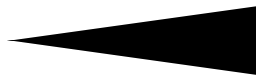
\includegraphics[width=0.5cm]{img/cssp/macros/newprec.png}}}}

\newcommand*\newtiltedprec{\vcenter{\hbox{\rotatebox{-30}{
\includegraphics[width=0.5cm]{img/cssp/macros/newtiltedprec.png}}}}}
% Definitions of handy macros can go here



% Expectation symbol

%\DeclareRobustCommand{\bbone}{\text{\usefont{U}{bbold}{m}{n}1}}


% Heading arguments are {volume}{year}{pages}{date submitted}{date published}{paper id}{author-full-names}



% Short headings should be running head and authors last names

%\firstpageno{1}

\begin{document}

\title{Thesis manuscript}


\author{Ayoub Belhadji} %if necessary, replace with your course title
 
\maketitle
%\author{\name Authors}

%\editor{Editors}

%\maketitle

%\begin{abstract}%   <- trailing '%' for backward compatibility of .sty file
%aaa
%\end{abstract}



\newpage
%\section{Introduction en français}
\chapter{Introduction}\label{chap:introduction}
%\subsection{Sensing on budget} 
%data analysis, signal processing or machine learning


Many tasks in applied mathematics can be reformulated as problems of sensing under budget constraints, that is the estimation of some function of the data based on a partial knowledge of the available data; this function can be a scalar, a vector, a matrix or even an function. Examples of these sensing problems include subset selection, numerical integration or interpolation. 

The aim of a subset selection algorithm is to approximate a finite dimensional object (scalar, vector or matrix) that is defined on a large set using only a small subset. This class of approximations are conducted, mainly, for three purposes: improving the numerical complexity of an existing algorithm, reducing the cost of labeling for a supervised learning algorithm or making an algorithm more interpretable.
A large class of subset selection algorithms deal with linear algebra operations; and for this class of algorithms the object to be approximated have an additive structure and the task usually boils down to approximating a large sum of scalars, vectors or matrices using a smaller sum. This additive structure can be also found in numerical integration problems and interpolation problems of elements of a Hilbert space. These tasks aim to approximate a function defined on some domain using few evaluations of this function that is usually an infinite dimensional object, and boils down to the approximation of an infinite sum using a finite sum.
%tool used offer a strong
% the object to approximate 
% have, usually,  related to the ....
% Among all the subset selection algorithms, those who deal  are the most studied. 
 % informational or  approximation can be benfical from 

% On the other hand, numerical integration and interpolation aim to approximate a function defined on some domain using few evaluations of this function that is usually an infinite dimensional object. Now, when the function is assumed to belong to some Hilbert space, we recover again an object with an additive structure. 


Randomization is usually used for sub sampling for its versatility and its strong theoretical guarantees. These guarantees are based on probabilistic inequalities that were the object of intense research since .... In particular, operator concentration inequalities are the culmination of this line of research.
A major question when working with randomized sums is to control the variance of this sum.


 % The approximation 

% concern the approximation of a function  Numerical integration 
%are also problems of sensing under budget. These problems

% Numerical integration is another problem of sensing under budget, it deals with the numerical approximation of intractable integrals. This problem exists, at least, since the invention of calculus???. Since then, several approaches were proposed for approximating integrals: Gaussian quadrature, Monte Carlo methods, Quasi-Monte Carlo methods and recently kernel methods. This variety of approaches reflects  main challenge for numerical integration problems 


% Interpolation problems are closely tied to numerical integration problems. These connections, between the two fields, did not prevent the first one to develop in its own way especially for questions emerging in numerical communication. The case of Whittaker–Shannon–Kotelnikov sampling theory is an example of such independent development.

Indeed, one may expect to reduce the sensing budget if the design avoids redundancy and allows to capture the essential of the information. 

The negative correlation property manifested by this probabilistic models seems appealing to use in design problems.
This thesis is devoted to investigate the suitability of using determinantal point processes as models for randomized sensing.


% Recently, a new class of probabilistic models were studied mnew class of sensing algorithms emerged for the study of these problems.


% When dealing with such approximation problems, The main concern in the developpemnt of these approximation schemes is the numerical implementation and the theoretical

% % . Many algorithms were proposed



% In particular, algorithms that are optimal in some sense are sought ...

% A plausible solution of one of these approximation problems is an algorithm that...



% This thesis studies determinantal point processes as a universal tool for subsampling. 


 Determinantal Point Processes (DPPs) were introduced by \cite{Mac75} as probabilistic models for beams of fermions in quantum optics. Since then, DPPs have been thoroughly studied in random matrix theory \citep{Joh05}, and have more recently been adopted in machine learning \citep*{KuTa12}, spatial statistics \citep*{LaMoRu15}, and Monte Carlo methods \citep{BaHa16}.
% a large class of DPPs 
The negative correlation property manifested by this probabilistic models seems appealing to use in design problems. Indeed, one may expect to reduce the sensing budget if the design avoids redundancy and allows to capture the essential of the information. 
Another appealing aspect about DPPs is numerical: the numerical simulation of these probabilistic models is tractable and witnessed many promising developments recently.
% several simulation algorithms were proposed recently the possibility of numerically simulate these probabilistic models as several numerical simulation algorithms were proposed and analyzed recently. 
This make DPP-based algorithms amenable to empirical testing.
 


A brief introduction to the theory of DPPs is given in the following. As a probabilistic model, DPPs appear in two forms: discrete DPPs and continuous DPPs. This does not prevent us from giving a unified definition of the two forms. We shall see in the end of this section that these two forms deal with two different approximation problems. Moreover, the two forms diverges regarding the efficiency of the numerical simulations.

In order to situate the contributions of this thesis, a brief review on matrix sparsification and operator discretization is given in the following.


 % we give a very brief review on  matrix sparsification techniques and ......
%in Design problems in applied mathematics
\section{Subsampling problems}

 %  that can be decomposed as aggolmeration of 

 % usually  initially were used for the pre-conditioning of linear solvers \citep{Golub1965} [???] that is purely a numerical routine in numerical linear algebra. Yet, the use of the subset selection paradigm expanded and covered different problems in various settings: coresets for a learning task, subset selection in numerical linear algebra especially for regression tasks and for efficient factorization of gram kernel matrices, signal recovery on graphs, low rank factorization of matrices, efficient implementations of Bayesian inference based on MCMC algorithms...

\subsubsection{Matrix sparsification}
The problem of matrix sparsification is at the heart of many applications in data analysis and machine learning: pre-conditioning of linear systems (solvers) \citep{Golub1965}, subsampling for linear regression \citep*{DrMaMu06}, low rank approximations \citep*{DrMaMu07}, low-rank kernel matrix approximations \citep{Bac13,AlMa15}, linear systems on graphs \citep*{SpTe04,SpSr11} and signal recovery on graphs \citep*{PuTrGrVa18}. All these problems start with an s.d.p matrix that writes
\begin{equation}
\bm{M} = \sum\limits_{n \in [N]} v_{n}v_{n}^{\Tran},
\end{equation}
and it is required to sparsify $\bm{M}$ i.e. find a vector $\bm{w} \in \mathbb{R}^{N}$ such that the spectral properties of the matrix

\begin{equation}
\bm{M}_{\bm{w}} = \sum\limits_{n \in [N]} w_{n} v_{n}v_{n}^{\Tran},
\end{equation}
are similar to the spectral properties of $\bm{M}$ with the constraint that the size of the support of $\bm{w}$ , $|\{ i \in [N]; w_{i} \neq 0 \}|$ is as small as possible. 
The vectors $v_{n}$ may have different interpretation depending on the context of the problem. For example, in the context of linear regression on budget, $N$ is the number of initial observations that lives in dimension $d$, the $v_{i}$ are the observations, and $\bm{M}$ is the empirical covariance matrix. Graph sparsification offers another example of this setting; here the $v_{i}$ represents the edges and $d$ is the number of vertices and $\bm{M}$ is the Laplacian matrix.




The similarity between $\bm{M}_{\bm{w}}$ and $\bm{M}$ are measured by the similarity of the respective eigenvalues, a condition that can be formalized using the Loewner order: $\bm{M}_{\bm{w}}$ and $\bm{M}$  are similar if there exists $\alpha,\beta>0$ such that

\begin{equation}\label{eq:matrix_similarity_condition}
\alpha \bm{M} \prec \bm{M}_{\bm{w}} \prec \beta \bm{M}.
\end{equation}
%and defines a class of "good" matrix sparsifiers.
% More interestingly, this condition implies
%thus guarantees
%respective 
This spectral similarity is essential 
and guarantees the preservation of many other "spectral quantities" related to the initial matrix $\bm{M}$. For example, the condition~\eqref{eq:matrix_similarity_condition} guarantees that the null-spaces of $\bm{M}$ and $\bm{M}_{\bm{w}}$ are the same, that $\rank(\bm{M}) = \rank(\bm{M}_{\bm{w}})$ and that the pseudo-inverses are similar \citep{MiAk77}
\begin{equation}
\frac{1}{\beta} \bm{M}^{+} \prec \bm{M}_{\bm{w}}^{+} \prec \frac{1}{\alpha} \bm{M}^{+}.
\end{equation}
Also, it guarantees that 
\begin{equation}
\forall \bm{x} \in \mathbb{R}^{d}, \:\:
\alpha \bm{x}^{\Tran}\bm{M}\bm{x} \leq \bm{x}^{\Tran}\bm{M}_{\bm{w}}\bm{x} \leq \beta \bm{x}^{\Tran}\bm{M}\bm{x}.
\end{equation}

the preservation of many other "spectral quantities" related to the initial matrix $\bm{M}$: flows ?? in graph 

% Now, assume for a moment that $\bm{M}$ is equal to the identity matrix $\mathbb{I}_{d}$. 




Now, the condition~\eqref{eq:matrix_similarity_condition} can be written as
\begin{equation}
\alpha \mathbb{I}_{d} \prec \bm{M}^{-1/2}\bm{M}_{\bm{w}} \bm{M}^{-1/2} \prec \beta \mathbb{I}_{d},
\end{equation}
with
\begin{equation}
 \bm{M}^{-1/2}\bm{M}_{\bm{w}} \bm{M}^{-1/2}  = \sum\limits_{n \in [N]} w_{n} \bm{M}^{-1/2} v_{n} (\bm{M}^{-1/2} v_{n})^{\Tran} = \sum\limits_{n \in [N]} w_{n} \tilde{v}_{n} \tilde{v}_{n}^{\Tran},
\end{equation}
where
\begin{equation}
\forall n \in [N], \:\:\tilde{v}_{n} = \bm{M}^{-1/2} v_{n}.
\end{equation}
Therefore, the problem of sparsfication of $\bm{M}$ boils down to the sparsification of $\mathbb{I}_{d}$
\begin{equation}\label{eq:sum_to_identity}
\mathbb{I}_{d} = \sum\limits_{n \in [N]}\tilde{v}_{n}\tilde{v}_{n}^{\Tran}.
\end{equation}

As an example of a randomized sparsification, we recall the following result.




\begin{theorem}\label{thm:matrix_bernstein_identity_sparsification}
Let $\tilde{v}_{1}, \dots, \tilde{v}_{N} \in \mathbb{R}^{d}$, that satisfy the condition~\eqref{eq:sum_to_identity}, and
$\bm{p} \in (\mathbb{R}_{+}^{*})^{N}$ such that
\begin{equation}
\sum\limits_{n \in [N]} p_{n} = 1.
\end{equation}
Let $c \in \mathbb{N}^{*}$, and define the matrix $\mathbb{I}_{d,c}~\in~\mathbb{R}^{d\times d}$ by
\begin{equation}
\mathbb{I}_{d,c} = \sum\limits_{j \in [c]} \frac{1}{p_{i(j)}}\tilde{v}_{i(j)}^{\phantom{\Tran}}\tilde{v}_{i(j)}^{\Tran},
\end{equation} 
where
% \begin{equation}\label{eq:conditions_on_the_vector_p}
% \sum\limits_{j} p_{j} = 1, \:\: p_{j}>0,
% \end{equation}
%and
the $(i(j))_{j \in [c]}$ are independent random variables that follows the multinomial distribution of parameter $\bm{p}$. Then
\begin{equation}
\EX \mathbb{I}_{d,c} = \mathbb{I}_{d},
\end{equation}
and for $\delta >0$
\begin{equation}
\Prb \bigg( \|\mathbb{I}_{d,c} - \mathbb{I}_{d}\|_{2} \bigg) \geq 
\end{equation}


% Let , and $c \geq d \log d ...$, then with probability higher than $1-\delta$,

% \begin{equation}
%  (1-\epsilon) \mathbb{I}_{d} \prec \bm{M}_{c} \prec (1+\epsilon) \mathbb{I}_{d}.
% \end{equation}

\end{theorem}

The matrix $\bm{M}_{c}$ in the theorem can be written as a sum $\displaystyle \sum\limits_{n \in [N]}w_{n}v_{n}v_{n}^{\Tran}$ where $|\mathrm{Supp}(\bm{w})|~=~...$ and it is indeed a sparsification of the identity matrix $\mathbb{I}_{d}$. Moreover, any vector $\bm{p}$ satisfying the two conditions~\eqref{eq:conditions_on_the_vector_p} can be used for sampling. Yet, the bound on the size of the support of $\bm{w}$ is only significant for a class of vectors $\bm{p}$. To see this, assume that $\bm{p} = (1/N)_{j \in [N]}$ that represents uniform sampling. Then, in order to obtain the guarantees of Theorem~\ref{thm:matrix_bernstein_identity_sparsification}, it is required to have  $c \geq ... d \log d $. When the \emph{coherence} $\mu$ is low $(\mu \approx 1)$, the sparsification is guaranteed with $\mathcal{O}(d \log d)$ independently of the initial number $N$. This reduction is significant, especially for large values of $N$. Yet, in the worst case $\mu = N$, and it is required that $c \geq N$. In other words, the sparsification using uniform sampling is only guaranteed if the coherence is low.

We can see the issue with the uniform distribution 

\begin{equation}
...
\end{equation}

are interesting. To see this, consider $p$

 and as we have seen, the distribution of the elements of the support of $\bm{w}$ are chosen according to some multinomial distribution of parameter $\bm{p}$.

To summarize, random sampling allows to obtain almost optimal sparisifiers with a budget that scales as $\mathcal{O}(d \log d)$. The logarithmic term in the matrix concentration inequalities was shown to be almost optimal in [??]. 
In the following, we review a class of sparsifiers that achieves sparsification budget that scales as $\mathcal{O}(d)$.




% Consider the following problem: let $v_{1}, \dots, v_{N} \in \mathbb{R}^{d}$ such that
% \begin{equation}
%  \sum\limits_{n \in [N]} v_{n} v_{n}^{\Tran} = \mathbb{I}_{d},
% \end{equation}
% we ask for an algorithm that outputs a set $S \subset [N]$ and a vector of weights $\bm{w}\in \mathbb{R}^{N}$ such that
% \begin{equation}
% m \mathbb{I}_{d} \leq \sum\limits_{n \in [N]} w_{n}v_{n}v_{n}^{\Tran} \leq M \mathbb{I}_{d}.
% \end{equation} 


% The condition~\eqref{eq:sum_to_identity} 

% First let's comment the 


\paragraph{Random sparsification}
Random sampling algorithms are widely used in matrix sparsification. The popularity of these algorithms stems from the fact that they are relatively easy to implement and they benefits from strong theoretical guarantees.  Typically, the theoretical guarantees of such an algorithm goes through matrix concentration inequalities [??]. We give in the following an example of a matrix concentration inequality. 


\begin{theorem}\label{thm:matrix_bernstein}
Consider a finite sequence $(X_{j})_{j}$ of independent, random, self-adjoint $d\times d$ matrices . Assume that each matrix $X_{j}$
satisfies 
\begin{align}
 \EX X_{j} &= \mathbb{0}_{d \times d},\\
 \|X_{j}\|_{2} &\leq \tau,
\end{align}
where $\tau >0$ and define $\sigma^{2} = \|\EX \sum\limits_{j} X_{j}^{2}\|$.
% and 
% Let $\rho_{j} = \max(\|\EX X_{j} X_{j}^{\Tran}\|_{2}, \|\EX X_{j}^{\Tran}X_{j}\|_{2})$, and $\max\limits_{j \in [c]} $.
 Then for $\epsilon >0$, 

\begin{equation}
\Prb \left( \|\sum\limits_{j} X_{j}\|_{2} \geq \epsilon \right) \leq 2 d e^{-\frac{3}{2} \frac{\epsilon^{2}}{3\sigma^{2} + \tau \epsilon}}.
\end{equation}

\end{theorem}

This result is widely known under the name of \emph{Matrix Bernstein concentration inequality} because it is the natural extension of the Bernstein concentration inequality. Similarly, other scalar concentration inequalities extend to matrices. For instance, the Chernoff concentration inequality or the Azuma-Hoeffding concentration inequality. We refer the reader to [??] for a review on this topic. 

% matrix concentration inequalities that extend scalar concentration inequalities such as Matrix Chernoff concentration inequality or Matrix Azuma concentration inequality.


An application of Theorem~\ref{thm:matrix_bernstein} is the following sparsification result.


\paragraph{Greedy sparsification}
An alternative approach to sparisification was proposed in \citep*{BaSpSr12}. While the primary motivation of the authors was graph sparsification, they proved a general result for the sparisification of the identity matrix.
\begin{theorem}\citep*{BaSpSr12}
Let $v_{1}, \dots, v_{N} \in \mathbb{R}^{d}$ , that satisfies the condition~\eqref{eq:sum_to_identity}, and let $\alpha >1$. Then there exists $\bm{w} \in \mathbb{R}_{+}^{N}$ such that
\begin{equation}
\mathbb{I}_{d} \prec \sum\limits_{n \in [N]}w_{n}v_{n}v_{n}^{\Tran} \prec \frac{\alpha +1 +2\sqrt{\alpha}}{\alpha +1 -2\sqrt{\alpha}} \mathbb{I}_{d},
\end{equation}
and
\begin{equation}
|\{n \in [N], w_{n} \neq 0\}| \leq \alpha d.
\end{equation}
\end{theorem}


The proof given in \citep{BaSpSr12} provides a deterministic greedy algorithm for computing the vector $\bm{w}$ in $\mathcal{O}(\alpha d^{3} N)$ time. The proof is based on the following observation: let $\bm{A}$ a $d\times d$ p.s.d matrix and $v \in \mathbb{R}^{d}$, and denote $\pi_{\bm{A}}$,$\pi_{\bm{A}+vv^{\Tran}}$ the characteristic polynomials of the matrices $\bm{A}$ and $\bm{A}+vv^{\Tran}$ respectively, then 
\begin{equation}
\pi_{\bm{A}+vv^{\Tran}}(\lambda) =  \pi_{\bm{A}}(\lambda) \bigg( 1- \sum\limits_{\delta \in [d]} \frac{\langle v,u_{\delta} \rangle^{2}}{\lambda-\lambda_{\delta}} \bigg), 
\end{equation}
where the $\lambda_{\delta}$ are the eigenvalues of $\bm{A}$ and the $u_{\delta}$ are the respective eigenvectors.



control of the eigenvalues of the matrices ... under rank-one updates.


\subsection{Operator discretization}
(3-6 pages)
\section{Mathematical framework: Determinantal point processes}
(7-10 pages)
 

Before giving the definitions of DPPs, we recall some basic properties of determinant that are connected to the geometric notion of volume.

\subsection{The determinant and the volume}
We recall this elementary result:
\begin{theorem}\label{thm:link_det_vol}
Let $v_{1}, \dots, v_{d} \in \mathbb{R}^{d}$ a collection of vectors, and denote $\mathcal{P}$ the parallelepiped spanned by the $v_{\delta}$, i.e. the convex hull of $(v_{\delta})_{\delta \in [d]}$ and denote by $\bm{G}$ the gram matrix of the $v_{\delta}$. Then
\begin{equation}
\Det \bm{G} = \mathrm{Vol}^{2} \mathcal{P}. \nonumber
\end{equation}
\end{theorem}
Theorem~\ref{thm:link_det_vol} establishes the link between the geometric notion of volume and the determinant of Gram matrices: the higher the determinant of $\bm{G}$ the higher the volume of $\mathcal{P}$ and vice-versa. The volume of the parallelepiped $\mathcal{P}$ is a convenient 

One important, yet elementary, consequence of Theorem~\ref{thm:link_det_vol} is the 


\begin{theorem}\label{thm:vol_base_times_height}
Let $v_{1}, \dots, v_{d} \in \mathbb{R}^{d}$ a collection of vectors, and denote $\mathcal{P}$ the parallelepiped spanned by the $v_{\delta}$, i.e. the convex hull of $(v_{\delta})_{\delta \in [d]}$ and denote by $\bm{G}$ the gram matrix of the $v_{\delta}$. Then
\begin{equation}
\Det \bm{G} = \mathrm{Vol}^{2} \mathcal{P}. \nonumber
\end{equation}
\end{theorem}

% Wh a unified definition can be given for these two forms,  can be defined using the same mathematical framework; the accomplished tasks are fundamentally different.





\subsection{Definitions}
Before giving the definition of a determinantal point process, we recall briefly the definition of a point process, and we refer to Appendix ?? for further details on this topic.

Intuitively, a point process is a random subset on some set $\X$. Examples of $\X$ include discrete sets (finite or infinite), $\mathbb{R}^{d}$ or some subset of $\mathbb{R}^{d}$ or the hypersphere $\mathbb{S}^{d-1}$. Keeping these examples in mind, we can assume that $\X$ is a separable Hausdorff space.


First, we give the definition of a point process. 

\begin{definition}
A configuration of $\X$ is a subset $\gamma$ of $\X$ that satisfies the following conditions:
\begin{itemize}
\item $\gamma$ is discrete 
\item for every compact subset $\mathcal{K}$ of $\X, \: |\gamma \cap \mathcal{K}| < +\infty $.

\end{itemize}
We denote by $\Gamma$ the set of configurations on $\X$.
\end{definition}

Denote by $\mathcal{G}$, the $\sigma$-algebra generated by the sets 
\begin{equation}
\{\gamma \in \Gamma, \: |\gamma \cap \mathcal{K}| = m \},
\end{equation}
where $\mathcal{K}$ is a compact set of $\X$ and $m \in \mathbb{N}$.



\begin{definition}
A point process $\gamma$ is a measurable application from a measure space into $(\Gamma, \mathcal{G})$.
\end{definition}

In other words, a point process is a random configuration.  

\begin{definition}
Let $\gamma$ be a point process on $\X$, and $n \in \mathbb{N}^{*}$. If there exists a non-negative function $\rho_{n}: \X^{n} \rightarrow \mathbb{R} $ satisfying 
\begin{equation}\label{eq:def_joint_intensity}
\EX \sum\limits_{(x_{1}, \dots, x_{n}) \in \gamma } f(x_{1}, \dots, x_{n}) = \frac{1}{N!} \int_{\X^{N}} f(x_{1}, \dots, x_{n}) \rho_{n}(x_{1}, \dots, x_{n}) \otimes_{i \in [n]} \mathrm{d}\omega(x_{i}),
\end{equation}
for all .... functions $f$, then $\rho_{n}$ is called the $n$-order joint intensity function of $\gamma$.
\end{definition}
By considering a test function $f = \mathbb{1}_{\mathcal{B}}$, \eqref{eq:def_joint_intensity} is equivalent to 
\begin{equation}
\Prb \bigg(\big(x_{1}, \dots, x_{n} \big) \in \mathcal{B} \bigg) = \int_{\mathcal{B}} \rho_{n}(x_{1}, \dots, x_{n}) \otimes_{i \in [n]}\mathrm{d}\omega(x_{i}).
\end{equation}
In other words, $\rho_{n}(x_{1}, \dots, x_{n}) \otimes_{i \in [n]}\mathrm{d}\omega(x_{i})$ is the probability of the event $\big(x_{1}, \dots, x_{n} \big)...$...
In the case $n = 1$, $\rho$

We refer to [??] for further properties on point processes.


A DPP is a point process such that have $n$-order joint intensities, and those intensities are expressed with respect to some kernel $\kappa$.
\begin{definition}\label{eq:def_dpp}
Let $\gamma$ be a point process. $\gamma$ is said to be a determinantal point process on $\X$ with respect to the kernel $\kappa$ and the reference measure $\mathrm{d}\omega$ if its joint densities exist and satisfy
\begin{equation}
\rho_{n}(x_{1}, \dots, x_{N}) = \Det \bm{\kappa}(\bm{x}),
\end{equation}
where
\begin{equation}
\bm{\kappa}(\bm{x}) = (\kappa(x_{n},x_{n'}))_{n,n' \in [N]}.
\end{equation}
\end{definition}

In the definition~\eqref{eq:def_dpp}, the kernel $\kappa$ governs the statistical properties of the point process $\gamma$. For instance, if $n =1$, ...


\clearpage



\section{The layout and the contributions}
This thesis aims to investigate the use of determinantal point processes and their variants for subset selection problems and operator discretization. 

% The major technical contribution of this article 
A major contribution of this thesis is to highlight the importance of geometric parameters called the principal angles between subspaces in the theoretical analysis. Besides their geometric intuition, the introduction of these parameters enables closed form calculation of some upper bounds of the expected value of the approximation error under the projection DPP distribution. This approach was showed to be valid in both settings: discrete and continuous.

Another technical contribution is the introduction of a new technique of the analysis of kernel interpolation based on the perturbation of the eigenvalues of a Mercer kernel.
 % We show that this principal angles appear simultaneously on the the terms of approximation error and in the projection DPP. 



The chapters of this thesis are organized as follows:
\subsubsection{Projection DPPs for column subset selection}
A contribution concerns a new column subset selection algorithm for low rank factorization based on a projection DPP. 
In particular, we compare a particular projection DPP with volume sampling, a well-known distribution in the literature, and we prove that this projection DPP can lead to better theoretical guarantees and empirical results under a condition called \emph{the sparsity of the $k$-leverage scores}. Moreover, we prove theoretical guarantees under the more a realistic condition called \emph{the relaxed sparsity of the $k$-leverage scores}. Interestingly, the introduction of these notions of sparsity is inspired by a geometric analysis of worst case that was previously used to prove a lower bound of this class of algorithm CSPPs in [??]: the novel analysis we introduce, proves that it is possible to bypass this lower bound... These sparsity conditions were proved to be satisfied by several datasets. 
% Moreover, we check that these conditions are satisfied in several datasets. 

A major contribution of this chapter is to highlight the importance of geometric parameters called the principal angles between subspaces in the theoretical analysis. Besides their geometric intuition, the introduction of these parameters enables closed form calculation of some upper bounds of the expected value of the approximation error under the projection DPP distribution.
This new parametrization allows to give a simultaneous analysis under the Frobenius norm and the spectral norm. Moreover, the conducted analysis allows us to study the bias of regression using the selected features.

% The advantage of thisimprovement is expressed both using the Frobenius and the spectral norm. 


% Another interesting feature about this theoretical analysis is its ver


%  relaxed sparsity   on the sparisiy of show the influence of the choi using a specific choice of projection DPP, the theoretical guarantees  ac allows to improve both and the empirical results 
% on this settings deal with ....
% The first contribution of this thesis was to propose and analyse a . In fact, the initial objective was to understand whether the well-known result on the litterature is improvable.

% \begin{theorem}[\citealp{DRVW06}]
%   \label{thrm:volume_sampling_theorem_introduction}
% Let $S$ be a random subset of $[d]$, chosen with probability
% \begin{equation}
% \Prb_{\VS}(S) = Z^{-1} \,\Det(\bm{X}_{:,S}^{\Tran}\bm{X}_{:,S}^{})\, \mathbb{1}_{\{|S| = k \}},
% \label{e:vs}
% \end{equation}
% where $Z = \sum\limits_{|S| = k} \Det(\bm{X}_{:,S}^{\Tran}\bm{X}_{:,S}^{})$.
% Then
% \begin{equation}
% \EX_{\VS} \| \bm{X} - \Pi_{S}^{\Fr}\bm{X} \|_{\Fr}^{2} \leq (k+1)\| \bm{X} - \Pi_{k}\bm{X} \|_{\Fr}^{2}
% \label{e:vsBoundFr}
% \end{equation}
% and
% \begin{equation}
% \EX_{\VS} \| \bm{X} - \Pi_{S}^{2}\bm{X} \|_{2}^{2} \leq (d-k)(k+1)\| \bm{X} - \Pi_{k}\bm{X} \|_{\Fr}^{2} .
% \label{e:vsBound2}
% \end{equation}
% \end{theorem}

%  that allow us to propose a column subset selection algorithm based on a projection DPP that improves on volume sampling under some conditions. 

\subsubsection{DPPs for kernel quadrature}

In this work we proposed to analyze optimal kernel quadratures based on nodes that follows the distribution of projection DPP. 
In this work we leverage the intuitions developed in the previous work to work out the theoretical analysis of the algorithm. More precisely, we prove that once again, principal angles can be used in the analysis of the approximation error ...

In particular, we highlight the importance of the eigenvalues of integration operators on the convergence rates in a similar fashion than the work of ??



\begin{table}
\centering
 \begin{tabular}{| c| c| c| c|}
 \hline
  Distribution/ Setting & Matrix & Operator\\
 \hline
 Projection DPP& \cite{BeBaCh18} & \cite{BeBaCh19} \\
 \hline
 Volume sampling& \cite{DRVW06} & ... \\
 \hline
 R-leverage scores & \cite{Bac13}  & \cite{Bac17}  \\
 &  \cite{AlMa15} &   \\
\hline
\end{tabular}
\caption{....\label{table:matrix_operator_duality}}
\end{table}


\subsubsection{Volume sampling for kernel interpolation}
In this work, we continue the line of research initiated in [??] and we prove that continuous volume sampling (the continuous version of the algorithm proposed by ??) into kernel quadrature and kernel interpolation.

In particular, we show closed formulas for the expected interpolation error under the distribution of the continuous volume sampling ....

These closed formulas allow us to prove sharp upper bounds ... In particular, we prove the optimality...

\subsubsection{Applications in signal processing}
\subsubsection{The richest Hermite kernel}
(2 pages)

\clearpage
\chapter{Determinantal point processes}\label{chapter:dpp}

This chapter is dedicated to give a formal introduction on determinantal point processes. As it was mentioned in the Introduction, these probabilistic models appear mainly in two forms: discrete DPPs and continuous DPPs. We shall give an abstract definition that includes the two settings, thereafter we instantiate this definition to highlight the differences between them. For this reason, we adopted a different notation in this chapter that will change in the next chapters. The rationale behind this choice is to keep the notation as close as possible to the usual ones in the corresponding literatures.

We start by recalling some elements of the theory of point processes, that is the natural framework where DPPs are defined, in Section~\ref{sec:pointprocesses}; then we give the definition of a DPP and some basic notions and results on the theory in Section~\ref{sec:dpp_defs}. In particular, we give several examples of DPPs in Section~\ref{sec:DPP_examples} and we recall the HKPV algorithm, for the numerical simulation of a DPP, in Section~\ref{sec:num_algos_dpps}.


% The definition of a DPP, given in  goes through the theory of point processes that we shall recall, briefly, the basics in Section~\ref{sec:pointprocesses}. Finally, Section~\ref{sec:num_algos_dpps} is dedicated for a review on numerical simulation algorithms of DPPs and their variations.

% Finally,  

% \section{A very brief history of DPPs} 

\section{Point processes}\label{sec:pointprocesses}

Intuitively, a point process is a random collection of isolated points in some set $\mathcal{D}$. In order to define such a concept within the usual framework of probability theory, it is more convenient to see a discrete subset of $\mathcal{D}$ as an atomic measure defined on $\mathcal{D}$. Indeed, the set of measures on $\mathcal{D}$ have properties that are compatible with the standard setting of probability theory. 


% the set of discrete subsets of $\mathcal{D}$ have to 



% In order to define such a concept within the usual framework of probability theory, $\mathcal{D}$ have to satisfy some conditions. 

Let $(\mathcal{D},\mathcal{T})$ be a topological space that is \emph{locally compact} (every point has a compact neighborhood), \emph{second countable} ($\mathcal{T}$ has a countable base) and \emph{Hausdorff} (for any two distinct points there exist neighborhoods of each point that are disjoint).
 These three conditions guarantee that $(\mathcal{D},\mathcal{T})$ is a Polish space, that is there exists some metric $d$ on $\mathcal{D}$ such that the
topology induced by $d$ is equal to $\mathcal{T}$ and $(\mathcal{D},d)$ is a \emph{complete} and \emph{separable} (there is a countable set $\{x_{n}; n \in \mathbb{N}\}$ that is dense in $\mathcal{D}$)
metric space; see Theorem 5.3 in \citep{Kec95}.
% First, we assume that $(\mathcal{D},d)$ is a metric space for some metric $d$. 
\begin{example}
We recall some examples of a Polish space.
\begin{itemize}
\item A countable set with the discrete topology is a Polish space, 
\item The sets $\mathbb{R}^{d}, \mathbb{C}^{d}$ with $d \in \mathbb{N}^{*}$ with the respective usual topologies are Polish spaces,
\item A closed subspace of a Polish space is a Polish space; see Proposition 3.3 in \citep{Kec95}.
\item Manifolds [??]
\end{itemize}
% discrete sets endowed by the discrete metric, subsets of $\mathbb{R}^{d}$ with the Euclidean distance, manifolds ...????
\end{example}

Define $\mathcal{B}$ to be the Borel $\sigma$-algebra: the smallest $\sigma$-algebra in $\mathcal{D}$ that contains all open subsets of $\mathcal{D}$. Its elements are called Borel sets. A measure $\mu$ is a function from $\mathcal{B}$ to $\mathbb{R}_{+} \cup \{\infty \}$ that is \emph{non-negative}, $\sigma$-\emph{additive} and vanishes at the empty set. A locally finite measure is a measure $\mu$ on $(\mathcal{D},\mathcal{B})$ such that for every compact set $C$ of $\mathcal{D}$
\begin{equation}
\mu(C) <+\infty.
\end{equation}
Denote by $\mathbf{M}(\mathcal{D})$ the set of locally finite measures.
% This assumption is not restrictive, as it includes a wide class of sets:  
% Moreover, we assume that $(\Omega,d)$ is complete, and separable: . This condition insures that 
%  make this definition rigorous, some conditions on $\Omega$ will be assumed. 
% Informally, a point process is a random discret subset of some set $\Omega$. A rigorous definition requires to define a sample space that contains all discrete subsets of $\Omega$; and, as it is usually done in probability theory, this sample space is assumed to be a complete separable metric space. 
% The space of $\sigma$-finite Borel measures on $\Omega$, denoted $M(\Omega)$, is a complete separable metric space if and only if $\Omega$ is a complete separable metric space \citep{Par05}??.
% We assume in the rest of the manuscript that this condition on $\Omega$ is satisfied. Indeed, this condition is more than sufficient for all the settings that we consider: it is easy to prove that dis...
%A measure $\mathcal{D}$ is 
We supply $\mathbf{M}(\mathcal{D})$ with the $\sigma$-algebra $\mathcal{M}(\mathcal{D})$ generated by the evaluation maps defined for every Borel set $B \in \mathcal{B}$
\begin{align}
\Phi_{B}: M(\mathcal{D}) &\rightarrow \mathbb{R}_{+}\cup \{\infty \}. \nonumber\\
\mu & \mapsto \mu(B) \nonumber
\end{align}

In other words, $\mathcal{M}(\mathcal{D})$ is the smallest $\sigma$-algebra for which all the evaluations maps $\Phi_{B}$ are measurables. This $\sigma$-algebra is generated by the cylinder sets (Lemma 3.1.1 in \citep{ScWe08})

\begin{equation}
\Big\{ \mu \in \mathbf{M}(\mathcal{D}), \:\: \mu(B_{1}) \in [0,r_1], \dots, \mu(B_{m}) \in [0,r_m] \Big\},
\end{equation}
where $m \in \mathbb{N}^{*}$, $B_{1}, \dots, B_{m}$ are open relatively compact subsets of $\mathcal{D}$ and $r_{1}, \dots, r_{m} \in \mathbb{R}_{+}$.



The set of counting measures defined by
\begin{equation}
\mathbf{N}(\mathcal{D}) = \Big\{ \mu \in \mathbf{M}(\mathcal{D}); \:\: \forall B \in \mathcal{B}, \mu(B) \in \mathbb{N}\cup \{+\infty\} \Big\}
\end{equation}
is an example  of an element of $\mathcal{M}(\mathcal{D})$; see Lemma 3.1.2 in \citep{ScWe08}.
%  an element $\mu$ of $\mathbf{N}(\Omega)$ takes values on $\mathbb{N}$
% \begin{equation}
% \mu(B) \in \mathbb{N}.
% \end{equation}
% Indeed, we have the following result.
% \begin{proposition}
% We have $\mathbf{N}(\Omega) \in \mathcal{M}(\Omega)$ and the trace $\sigma$-algebra
% \begin{equation}
% \mathcal{N}(\Omega) = \bigg\{ \mathbf{N}(\Omega) \cap M; M \in \mathcal{M}(\Omega)\bigg\}
% \end{equation}
%  is generated by the system
% \begin{equation}
% ....
% \end{equation}
% \end{proposition}
% An important subset of $M^{+}(\Omega)$ 
% A counting measure $\mu$ is said to be simple if it takes values on $\{0,1\}$
% \begin{equation}
% \mu(B) \in \{0,1\}.
% \end{equation}
Another example is given by the set of simple counting measures Lemma 3.1.4 in \citep{ScWe08}
\begin{equation}
\mathbf{N}_{s}(\mathcal{D}) = \Big\{ \mu \in \mathbf{M}(\mathcal{D}); \:\: \forall x \in \mathcal{D}, \mu(\{x\}) \in \{0,1\} \Big\}.
\end{equation}
% We refer to Lemma 3.1.2 and  for the proofs that $\mathbf{N}(\mathcal{D})$ and $\mathbf{N}_{s}(\mathcal{D})$ (are you sure????) belong to $\mathcal{M}(\mathcal{D})$.

Starting from a collection of points $x_{1}, \dots, x_{N}$ in $\mathcal{D}$, one can define a counting measure
\begin{equation}
\mu = \sum\limits_{n \in [N]}\delta_{x_n},
\end{equation}
where
$$
\delta_{x}(A) = \left\{
    \begin{array}{ll}
     1 & \text{ if } x\in A\\
0 & \text{ otherwise}.
\end{array}
\right.
$$

In this case, $\mu \in \mathbf{N}_s(\mathcal{D})$ if and only if the $x_{n}$ are pairwise distinct; and $\mu$ can be identified to a the subset $\{x_{1}, \dots, x_{N}\}$. In particular, we will several notations that express this identification as summarized in Table~\ref{table:set_counting_measure_dictionary}.
\begin{table}
\centering
 \begin{tabular}{| c| c|}
 \hline
  $\gamma$ as a subset & $\gamma$ as a counting measure\\
 \hline
 $x \in \gamma$ & $\gamma(\{x\}) = 1$\\
 \hline
 $\{ x_1, \dots, x_{N} \} \subset \gamma$ & $\gamma(\{ x_1, \dots, x_{N} \}) = N$\\
 \hline
  $|\gamma| = M$ & $\gamma(\mathcal{D}) = M$\\
\hline
  $\gamma \cap C = \emptyset$ & $\gamma(C) = 0$\\
 \hline
  $|\gamma \cap C| = M$ & $\gamma(C) = M$\\
 \hline
\end{tabular}
\caption{A dictionary of notations.\label{table:set_counting_measure_dictionary}}
\end{table}
% use the notation $x \in \mu$ to express that $\mu (\{x\}) =1$. 
Otherwise, $\mu$ can be seen as as a discrete subset of $\mathcal{D}$ with multiplicities.
% Discrete subsets of $\Omega$ can be identified to simple counting measures by considering the corresponding atomic measures. Thereby, general counting measures can be seen as discrete subsets with multiplicities. 
% In this manuscript, we will be mostly interested in simple counting measures; even tough we give ...

% Now, we move to the definition of $\sigma$-algebras on the sets $\mathbf{M}(\Omega)$, $\mathbf{M}^{+}(\Omega)$, $\mathbf{N}(\Omega)$ and finally $\mathbf{N}_{s}(\Omega)$. 


% However, in general, a counting measure does not correspond to a discrete subset of $\Omega$.
% Any discrete subset $\bm{x} = \{x_{1}, \dots, x_{N}\}$ of $\Omega$ can be identified to  a simple counting measure: $\sum\limits_{n \in [N]} \delta_{x_{n}}$. Counting measures are stric

\begin{definition}
A random measure $\gamma$ on $\mathcal{D}$ is a measurable map from some probability space $(\Omega, \mathcal{A}, \mathbb{P})$  into the measurable space $(\mathbf{M}(\mathcal{D}), \mathcal{M}(\mathcal{D}))$. The distribution of $\gamma$ is given by the probability measure $\mathbb{P}_{\gamma}$ defined on $\mathcal{M}(\mathcal{D})$ by
\begin{equation}
\forall M \in \mathcal{M}(\mathcal{D}), \:\mathbb{P}_{\gamma}(M) = \mathbb{P}(\gamma \in M).
\end{equation}

% process $\gamma$ on $\Omega$ is a random positive Radon measure
% on $\Omega$ that takes values on $\mathbb{N}$ a.s.
\end{definition}

Any random measure $\gamma$ on $\mathcal{D}$ defines a stochastic process with values in $\mathbb{R}_{+}$ indexed by $\mathcal{B}$: $\{\gamma(B)\}_{B \in \mathcal{B}}$; see Proposition  1.1.7. in \citep*{BaBlKa20}.

\begin{definition}
A point process $\gamma$ on $\mathcal{D}$ is a random measure on $\mathcal{D}$ such that
\begin{equation}
\mathbb{P}_{\gamma} \big(\mathbf{N} (\mathcal{D}) \big) = 1.
\end{equation}
The point process $\gamma$ is said to be a simple if 
\begin{equation}
\mathbb{P}_{\gamma}\big(\mathbf{N}_{s}(\mathcal{D})\big) = 1.
\end{equation}
% that is $\gamma$ takes values in $\{0,1\}$.
% positive Radon measure
% on $\Omega$ that takes values on $\mathbb{N}$ a.s.\\

\end{definition}

%\begin{example}
Consider the following example. Let $\mu$ be a probability measure on $\mathcal{D}$ and let $\nu$ be a probability measure on $\mathbb{N}$. Let $x_{0}, x_{1} \dots, $ be independent random variables that follow the distribution $\mu$ and $N$ a random variable that follows the distribution $\nu$.
Then the random measure $\gamma$ defined by
\begin{equation}
\gamma = \sum\limits_{n \in [N]} \delta_{x_{n}},
\end{equation}
is a point process on $\mathcal{D}$. This point process is called the \emph{mixed binomial process} with mixing distribution $\nu$ and sampling distribution $\mu$.
Now, if  $\nu = \delta_{N_0}$ for some $N_0 \in \mathbb{N}^{*}$, we recover the binomial process defined by
\begin{equation}\label{eq:binomial_cylinder_prb}
\forall B \in \mathcal{B}, \:\:\forall n \in \{0, \dots, N_0\}, \:\: \mathbb{P}(\gamma(B) = n) = \binom{N_0}{n}\mu(B)^{n}(1-\mu(B))^{N_0-n}.
\end{equation}
On the other hand, if $\nu$ follows the distribution of a Poisson random variable of parameter $1$, then we recover a Poisson point process of intensity $\mu$ that we define in the following.
% \begin{equation}
% \forall n \in \mathbb{N}, \:\: \mathbb{P}(\gamma(B) = n) = e^{-\lambda \mu(B)}\frac{(\lambda \mu(B))^{n}}{n!}.
% \end{equation}
%\end{example}
\begin{definition}
Let $\mu$ be a measure on $\mathcal{D}$. A Poisson process with intensity measure $\mu$ is a point process $\gamma$  that satisfies the following properties
\begin{itemize}
\item for every $B \in \mathcal{B}$, $\gamma(B)$ follows the distribution of a Poisson random variable of parameter $\mu(B)$,
\item for every $B_{1}, \dots, B_{m} \in \mathcal{B}$ pairwise disjoint Borel sets, the random variables $\gamma(B_{1}), \dots, \gamma(B_{m})$ are independent. 
\end{itemize}
\end{definition}

In other words, under a Poisson point process of intensity $\mu$, for every $B_{1}, \dots, B_{m} \in \mathcal{B}$ pairwise disjoint Borel sets, and $n_{1}, \dots, n_{m} \in \mathbb{N}$
\begin{equation}\label{eq:poisson_cylinder_prb}
\mathbb{P} \Big(\gamma(B_{1}) = n_{1}, \dots, \gamma(B_{m}) = n_{m} \Big) = e^{- \mu(B_{1})}\frac{ \mu(B_{1})^{n_1}}{n_{1}!} \times \dots \times e^{- \mu(B_{m})}\frac{ \mu(B_{m})^{n_m}}{n_{m}!} .
\end{equation}

% The following variation of Binomial process generate a rich family of point processes called \emph{Poisson point processes.}
The description of a point process through cylinder sets $\{ \gamma(B) = n \}$ is convenient in some cases such as the binomial process and the Poisson point process. However, in general,
\begin{equation}
\mathbb{P} \Big(\gamma(B_{1}) = n_{1}, \dots, \gamma(B_{m}) = n_{m} \Big)
\end{equation}
have no tractable formula and it is more convenient to work with an alternative description offered by the moment measures that we will define in the following.
% Observe that in these two cases of mixed binomial process, the description of the point process through the cylinder sets  is tractable. This is not always the case and 
% The discription of a point process using cylinder sets 
%This alternative description is .
We start with the mean measure.  
\begin{definition}
Let $\gamma$ be a point process. The mean measure of $\gamma$ is the measure $\gamma_{1}$ defined by
\begin{equation}\label{eq:first_intensity_measure}
\forall B \in \mathcal{B}, \:\: \gamma_{1}(B) = \mathbb{E} \gamma(B).
\end{equation}
\end{definition}
The mean measure is well defined but may take infinite values. 
\begin{example}
Let $\gamma$ be a Poisson point process associated to an intensity $\mu$, where $\mu$ is a measure on $\mathcal{D}$. It is immediate from~\eqref{eq:poisson_cylinder_prb} that 
\begin{equation}
\forall B \in \mathcal{B}, \:\: \mathbb{E}\gamma(B) = \mu(B).
\end{equation}
Therefore, the mean measure of $\gamma$ is simply equal to $\mu$.

\end{example}



Now, if $\gamma_{1}$ is absolutely continuous with respect to $\mathrm{d}\omega$, then the Radon Nikodym derivative $\rho_{1}$ is called the \emph{first intensity function} and it satisfies
\begin{equation}\label{eq:first_intensity_function}
\forall B \in \mathcal{B}, \:\:\mathbb{E} \gamma(B) = \gamma_1(B) = \int_{B} \rho_{1}(x) \mathrm{d}\omega(x). 
\end{equation}
% The intuition behind~\eqref{eq:first_intensity_function} depend on $\Omega$. We give two examples.

\begin{example}\label{ex:rho_1_inclustion_probability_discret_set}
Let $\mathcal{D}$ be a finite set and define the counting measure $\mathrm{d}\omega = \sum\limits_{x \in \mathcal{D}} \delta_x$. Then, for a simple point process $\gamma$
\begin{align}
\gamma_1(B) & = \sum\limits_{n \in \mathbb{N}} \Prb(\gamma(B) = n) n\\
& = \sum\limits_{n \in \mathbb{N}} \Prb(\gamma(B) = n) \sum\limits_{b \in B} \Prb \big( \gamma(\{b\}) = 1| \gamma(B) = n \big) \nonumber\\
& = \sum\limits_{b \in B} \sum\limits_{n \in \mathbb{N}} \Prb(\gamma(B) = n)  \Prb \big( \gamma(\{b\}) = 1| \gamma(B) = n \big) \nonumber\\
& = \sum\limits_{b \in B}  \Prb \big( \gamma(\{b\}) = 1\big) \nonumber\\
& = \int_{B} \rho_{1}(x) \mathrm{d}\omega(x), \nonumber
\end{align}
where 
\begin{equation}
\rho_{1}(x) = \mathbb{P} \big(\gamma(\{x\}) = 1 \big).
\end{equation}
In other words, the intensity function of a simple point process is the inclusion probability $\mathbb{P} \big(x \in \gamma \big)$.

\end{example}


Now, given a simple point process $\gamma$, the identity~\eqref{eq:first_intensity_measure} can be rewritten 
\begin{equation}\label{eq:primitif_Campbell_identity}
\forall B \in \mathcal{B}, \:\:\int_{\mathcal{D}} \mathbb{1}_{B} \gamma_1 = \mathbb{E}\sum\limits_{x \in \gamma} \mathbb{1}_{B}(x).
\end{equation}
The measurable function $\mathbb{1}_{B}$ in the identity \eqref{eq:primitif_Campbell_identity} can be replaced by any nonnegative measurable function as it is shown in the following result.


\begin{theorem}[Campbell–Hardy theorem]
Let $\gamma$ be simple point process in $\mathcal{D}$, and let $f: \mathcal{D} \rightarrow \mathbb{R}$ be a nonnegative measurable function. Then  $\sum\limits_{x \in \gamma} f(x)$ is measurable and 
\begin{equation}
\int_{\mathcal{D}} f \gamma_1 = \mathbb{E}\sum\limits_{x \in \gamma} f(x).
\end{equation}
In particular, if $\gamma_1$ is absolutely continuous with respect to $\mathrm{d}\omega$, then
\begin{equation}
\int_{\mathcal{D}} f(x) \rho_1(x) \mathrm{d}\omega(x) = \mathbb{E}\sum\limits_{x \in \gamma} f(x).
\end{equation}


\end{theorem}

Observe that the Campbell theorem can be applied for general point processes: the term $\sum_{x \in \gamma} f(x)$ should be replaced by $\int_{\mathcal{D}} f \gamma$. Moreover, it can be extended to functions $f: \mathcal{D} \rightarrow \mathbb{R}$ that are integrable with respect to $\gamma_1$. See Theorem 1.2.5 in \citep{BaBlKa20} for a general statement and its proof.

% simpler di
%  can be described by
% its joint intensities
% Again, we can calculate the joint intensities $\rho_L$ for
The mean measure gives an idea of the random measure $\gamma$ evaluated on one Borel set $B \in \mathcal{B}$ yet it does not capture the correlations between the evaluation of $\gamma$ on a family of Borel sets $B_{1}, \dots, B_{L} \in \mathcal{B}$. There are many ways to estimate this interaction. For example, we can define the $L$-th power of $\gamma$ that is a point process on the measurable space $\mathcal{D}^{L}$, equipped with the product $\sigma$-algebra, defined by
\begin{equation}
\forall \prod\limits_{\ell \in [L]} B_{\ell} \in \mathcal{B}^{L}, \:\: \gamma^{\otimes_{L}}(\prod\limits_{\ell \in [L]} B_{\ell}) = \prod\limits_{\ell \in [L]} \gamma(B_{\ell}),
\end{equation}
and we consider the mean measure of  $\gamma^{\otimes_{L}}$ defined by
\begin{equation}
\gamma^{\otimes_{L}}_{1} \big(\prod\limits_{\ell \in [L]} B_\ell \big) = \EX  \gamma^{\otimes_{L}} \big(\prod\limits_{\ell \in [L]} B_\ell \big) = \EX   \prod\limits_{\ell \in [L]} \gamma(B_{\ell}).
\end{equation}

% give the statistical description of the evaluation of a point process $\gamma$ on a family of Borel sets $B_{1}, \dots, B_{L} \in \mathcal{B}$. For example, we can consider the measure $\gamma_{L}^{*}$ defined on the measurable space $(\Omega^{L}, \mathcal{B}^{L})$
% \begin{equation}
% \gamma_{L}^{*} \big( \prod\limits_{\ell \in [L]}B_\ell \big) = \EX \prod\limits_{\ell \in [L]} \gamma(B_\ell).
% \end{equation}

% Defined this way, $\gamma_{L}^{*}$ can be seen as the first intensity measure of the product point process $\gamma^{\otimes_{L}}$ defined on $\Omega^{L}$. 

%An alternative definition 
The measure $\gamma_{1}^{\otimes_{L}}$ is also called the $L$-th moment measure of $\gamma$. The definition of $\gamma^{\otimes_{L}}_{1}$ is straightforward, yet it is not convenient in the study of DPPs that will be presented later.  
% can be hard to manipulate due to the potential intersections between the Borel sets $B_{1}, \dots, B_{L}$. 
An alternative definition that is more compatible with the structure of DPPs is slightly more technical, and it is given in the following. 

Define 
% , less trivial, yet more convenient for , 
% definition would be to restrain the description of $\gamma$ to families of pairwise disjoint Borel subsets. This is done in the following way. Define the set 
\begin{equation}
\mathcal{D}_{\neq}^{L} = \{ (x_{1}, \dots, x_{L}) \in \mathcal{D}^{L}; \: \forall \ell,\ell' \in [L], \: x_{\ell} \neq x_{\ell^{'}} \}.
\end{equation}
The set $\mathcal{D}_{\neq}^{L}$ is an open set of $\mathcal{D}^{L}$ (equipped with the product topology), therefore $\mathcal{D}_{\neq}^{L} \in \mathcal{B}^{L}$; and we can define the restriction of the point process $\gamma^{\otimes_L}$ to $\mathcal{D}_{\neq}^{L}$, denoted $\gamma^{\otimes_{L}} \lfloor \mathcal{D}_{\neq}^{L}$, by
\begin{equation}
\gamma^{\otimes_{L}} \lfloor \mathcal{D}_{\neq}^{L} \big(\prod\limits_{\ell \in [L]} B_\ell \big) = \gamma^{\otimes_{L}} \big( \prod\limits_{\ell \in [L]} B_\ell \cap \mathcal{D}_{\neq}^{L}   \big).
\end{equation}
$\gamma^{\otimes_{L}} \lfloor \mathcal{D}_{\neq}^{L}$ is a point process on $\mathcal{D}^L$ and we can define its mean measure that we denote $\gamma_L$ 
\begin{equation}
\gamma_{L} \big(\prod\limits_{\ell \in [L]} B_{\ell} \big)  = \EX \gamma^{\otimes_{L}} \lfloor \mathcal{D}_{\neq}^{L} \big( \prod\limits_{\ell \in [L]} B_{\ell} \big) = \EX \gamma^{\otimes_{L}} \big( \prod\limits_{\ell \in [L]} B_\ell \cap \mathcal{D}_{\neq}^{L}   \big).
\end{equation}
%Defined this way, $\gamma_L$ is the first intensity measure of the point process $\gamma^{\otimes_{L}} \lfloor \Omega_{\neq}^{L}$; and
Now, by definition (of $\mathcal{D}_{\neq}^{L}$), if the $B_{1}, \dots, B_L$ are pairwise distinct, then 
\begin{equation}
\gamma_{L} \big(\prod\limits_{\ell \in [L]} B_{\ell} \big) = \EX \gamma^{\otimes_{L}} \big( \prod\limits_{\ell \in [L]} B_\ell \cap \mathcal{D}_{\neq}^{L}   \big) = \EX \gamma^{\otimes_{L}} \big( \prod\limits_{\ell \in [L]} B_{\ell} \big)  = \EX \prod\limits_{\ell \in [L]} \gamma(B_\ell).
\end{equation} 
Yet, the equality between $\gamma_{L} \big(\prod_{\ell \in [L]} B_{\ell} \big)$ and $\EX \prod_{\ell \in [L]} \gamma(B_\ell)$ is not valid in general, and this is  the main difference between the point process $\gamma^{\otimes_{L}}$ and the point process $\gamma^{\otimes_{L}} \lfloor \mathcal{D}_{\neq}^{L}$. This difference is better illustrated for simple point processes.


Let $\gamma$ be a simple point process, the two point processes $\gamma^{\otimes_{L}}$ and $\gamma^{\otimes_{L}} \lfloor \mathcal{D}_{\neq}^{L}$ are simple. Indeed, let $\prod\limits_{\ell \in [L]} \{x_{\ell} \} \subset \mathcal{D}^{L}$, we have by the simplicity of $\gamma$

\begin{equation}
\gamma^{\otimes_{L}} (\prod\limits_{\ell \in [L]} \{x_{\ell } \}) = \prod\limits_{\ell \in [L]} \gamma\big(\{x_{\ell } \} \big) \in \{0,1\} , \:\: \text{a.s.}
\end{equation}

As for $\gamma^{\otimes_{L}} \lfloor \mathcal{D}_{\neq}^{L}$, we have two cases: either $\prod\limits_{\ell \in [L]} \{x_{\ell} \} \subset \mathcal{D}_{\neq}^{L}$ or $\prod\limits_{\ell \in [L]} \{x_{\ell} \} \cap \mathcal{D}_{\neq}^{L} = \emptyset$. In the first case

\begin{equation}
\gamma^{\otimes_{L}} \lfloor \mathcal{D}_{\neq}^{L}(\prod\limits_{\ell \in [L]} \{x_{\ell } \}) = \gamma^{\otimes_{L}} (\prod\limits_{\ell \in [L]} \{x_{\ell } \}) = \prod\limits_{\ell \in [L]} \gamma(\{x_\ell \}) \in \{ 0,1\}.
\end{equation}
In the second case, 
\begin{equation}
\gamma^{\otimes_{L}} \lfloor \mathcal{D}_{\neq}^{L}(\prod\limits_{\ell \in [L]} \{x_{\ell } \}) = \gamma^{\otimes_{L}} (\emptyset) = 0 \in \{ 0,1\}.
\end{equation}


In other words, $\gamma^{\otimes_{L}} \lfloor \mathcal{D}_{\neq}^{L}$ excludes any family $(x_{1}, \dots, x_{L})$ that contains the same element more than once; this is not the case of $\gamma^{\otimes_{L}}$.



% Therefore, the Campbell theorem is valid for $\gamma^{\otimes_{L}} \lfloor \Omega_{\neq}^{L}$ too.


%Now, 
\begin{definition}
Let $\gamma$ be a simple point process.
If $\gamma_{L}$ is absolutely continuous with respect to $\mathrm{d}\omega^{\otimes_L}$, then the corresponding Radon Nikodym derivative $\rho_{L}$ can be defined and it is called the $L$-intensity function or the joint intensity function of order $L$. In particular, for any family of pairwise disjoint Borel subsets $B_{1}, \dots, B_{L} \in \mathcal{B}$
\begin{equation}\label{eq:pointprocess_intensity_L}
\mathbb{E} \prod\limits_{\ell \in [L]} \gamma(B_{\ell}) = \int_{\prod\limits_{\ell \in [L]}B_{\ell}} \rho_{L}(x_{1}, \dots, x_{L}) \mathrm{d}\omega(x_{1}) \dots \mathrm{d}\omega(x_{L}).
\end{equation}
% and satisfies
% \begin{equation}
% \rho_{L}(x_{1}, \dots, x_{L}) = 0,
% \end{equation}
% when $x_{\ell} = x_{\ell^{'}}$ for some $\ell \neq \ell^{'}$.
 \end{definition}


% Observe that the joint intensity function of order $L$ can vanish on $\Omega^{L} \smallsetminus \Omega_{\neq}^{L}$ as it is explained in the following example.



\begin{example}
Consider $\mathcal{D} = \mathbb{R}^{d}$ and $\mathrm{d}\omega$ is the Lebesgue measure; and assume that $\gamma$ is simple. Let $x_{1}, \dots ,x_{L} \in \mathcal{D}$ pairwise distinct and let $\epsilon >0$ such that the balls $B_{\epsilon}(x_{\ell})$, centered around the $x_\ell$ and of radii equal to $\epsilon$, are pairwise distinct. Under some assumptions on the point process $\gamma$, we can prove that (see Chapter 1 of \citep{HoKrPeVi09})
\begin{equation}
\rho_L(x_{1}, \dots, x_L) = \lim\limits_{ \epsilon \rightarrow 0} \frac{\mathbb{P}\bigg(\forall \ell \in [L], \:\: \gamma(B_{\epsilon}(x_{\ell})) = 1 \bigg)}{\mathrm{d}\omega \bigg(B_{\epsilon}(x_{\ell}) \bigg)}.
\end{equation}
\end{example}

%%%%%%%%%%%%%%%%%%%%%%%%
%%%%%%%%%%%%%%%%%%%%%%%%


%Now, if $\gamma_{L}$ is absolutely continuous with respect to $\mathrm{d}\omega^{\otimes_L}$, then the corresponding Radon Nikodym derivative $\rho_{L}$ can be defined and it is called the $L$-intensity function or the joint intensity function of order $L$.
%\begin{definition}
%Let $\gamma$ be a simple point process. The joint intensity of order $L \in \mathbb{N}^{*}$ of $\gamma$ with respect to $\mathrm{d}\omega$ is (if it exists) a function $\rho_{L}: \Omega^{L} \rightarrow [0,+\infty[$, such that for any family of pairwise disjoint Borel subsets $B_{1}, \dots, B_{L} \in \mathcal{B}$
%\begin{equation}\label{eq:pointprocess_intensity}
%\mathbb{E} \prod\limits_{\ell \in [L]} \gamma(B_{\ell}) = \int_{\prod\limits_{\ell \in [L]}B_{\ell}} \rho_{L}(x_{1}, \dots, x_{L}) \mathrm{d}\omega(x_{1}) \dots \mathrm{d}\omega(x_{L}),
%\end{equation}
%and satisfies
%\begin{equation}
%\rho_{L}(x_{1}, \dots, x_{L}) = 0,
%\end{equation}
%when $x_{\ell} = x_{\ell^{'}}$ for some $\ell \neq \ell^{'}$.
%\end{definition}

%%%%%%%%%%%%%%%%%%%%%
%%%%%%%%%%%%%%%%%%%%%



\begin{example}\label{ex:rho_L_inclustion_probability_discret_set}
Let $\mathcal{D}$ be a finite set and define the counting measure $\mathrm{d}\omega = \sum\limits_{x \in \mathcal{D}} \delta_x$; and we consider a simple point process $\gamma$. Using a similar analysis to the one in Example~\ref{ex:rho_1_inclustion_probability_discret_set}, we can prove that

\begin{equation}
\rho_{L}(x_{1}, \dots, x_{L}) = \mathbb{P} \big(\forall \ell \in [L], \:\: \gamma(\{x_\ell\}) = 1 \big).
\end{equation}
This can be rewritten as
\begin{equation}
\rho_{L}(x_{1}, \dots, x_{L}) = \mathbb{P} \big(\{x_{1}, \dots, x_{L} \} \subset \gamma \big).
\end{equation}
Again, $\rho_{L}(x_{1}, \dots, x_{L})$ can be interpreted as an inclusion probability.
\end{example}


% Therefore, the of $\gamma$ is simply equal to $\mu$.
The Campbell-Hardy theorem can be applied to the point process $\gamma^{\otimes_{L}} \lfloor \mathcal{D}_{\neq}^{L}$. By observing that, for a nonnegative measurable function $f: \mathcal{D}^{L} \rightarrow \mathbb{R}$, the sum
\begin{equation}\label{eq:sum_over_configurations_campbell}
\sum\limits_{(x_{1}, \dots, x_{L}) \in \gamma^{\otimes_{L}} \lfloor \mathcal{D}_{\neq}^{L}} f(x_{1}, \dots, x_{L})
\end{equation}
can be simplified to 
 % the sum~\eqref{eq:sum_over_configurations_campbell} can be simplified to 
\begin{equation}
\sum\limits_{\substack{(x_{1}, \dots, x_{L}) \in \gamma^{\otimes_{L}} \\ x_{\ell} \neq x_{\ell^{'}}}} f(x_{1}, \dots, x_{L}),
\end{equation}
we obtain the following result.
\begin{theorem}
Let $\gamma$ be simple point process in $\mathcal{D}$, and let $f: \mathcal{D}^{L} \rightarrow \mathbb{R}$ be a nonnegative measurable function. Then  
\begin{equation}
\sum\limits_{\substack{(x_{1}, \dots, x_{L}) \in \gamma^{\otimes_{L}} \\ x_{\ell} \neq x_{\ell^{'}}}} f(x_{1}, \dots, x_{L})
\end{equation}
is measurable and
\begin{equation}
\mathbb{E} \sum\limits_{\substack{(x_{1}, \dots, x_{L}) \in \gamma^{\otimes_{L}} \\ x_{\ell} \neq x_{\ell^{'}}}} f(x_{1}, \dots, x_{L}) = \int_{\mathcal{D}^{L}} f \gamma_{L}.
\end{equation}


In particular, if the joint intensity $\rho_L$ is defined
\begin{equation}
\mathbb{E}\sum\limits_{\substack{(x_{1}, \dots, x_{L}) \in \gamma^{\otimes_{L}} \\ x_{\ell} \neq x_{\ell^{'}}}} f(x_{1}, \dots, x_{L}) = \int_{\mathcal{D}^{L}} f(x_{1}, \dots, x_{L}) \rho_{L}(x_{1}, \dots, x_{L}) \mathrm{d}\omega(x_{1}) \times \dots \times \mathrm{d}\omega(x_{L}).
\end{equation}

\end{theorem}


%   For example, let $\gamma$ be a Poisson point process  It is immediate from~\eqref{eq:poisson_cylinder_prb} that 
% \begin{equation}

% \end{equation}


% and for a counting measure on $\Omega$ define
% \begin{align}
% \mu_{\neq}^{\otimes_L}(B_{1} \times \dots \times B_{L}) = \left\{
%     \begin{array}{ll}
%      \prod\limits_{\ell \in [L]}\mu(B_{\ell}) & \text{ if the $B_{\ell}$ are pairwise disjoint}\\
% 0 & \text{ otherwise}.
% \end{array}
% \right.
% \end{align}



% Define the measure $\gamma_{L}$ on $(\Omega^{L}, \mathcal{B}^{L})$ by



% This requires to 

% $B_{1}, \dots, B_{L}$ of $\Omega$



% $\gamma(B_1), \dots, \gamma(B_L)$ 


\begin{example}
Let $\gamma$ be a Poisson point process associated to an intensity $\mu$, where $\mu$ is a measure on $\Omega$. Let $B_{1}, \dots, B_{L} \in \mathcal{B}$ be pairwise disjoint Borel sets. \eqref{eq:poisson_cylinder_prb} yields
\begin{equation}\label{eq:ppp_orthogonality}
\gamma_{L}(\prod\limits_{\ell \in [L]} B_\ell) =  \mathbb{E} \prod\limits_{\ell \in [L]} \gamma(B_\ell) = \prod\limits_{\ell \in [L]}\mu(B_\ell).
\end{equation}
% We can even prove that 
% \begin{equation}
% \gamma_{L}(...) = \gamma_{1}()
% \end{equation}
\end{example}
The identity~\eqref{eq:ppp_orthogonality} reflects the independence of the random variables $\gamma(B_{1}), \dots, \gamma(B_L)$ when $\gamma$ follows the distribution of a Poisson point process. In other words, under the law of Poisson point process, there is no interaction between pairwise disjoint Borel sets.  This is to be compared to the correlations that appear under the distribution of a determinantal point process. This class of point processes will be introduced in the following section.
% A process that satisfies the property \eqref{eq:ppp_orthogonality} is sometimes called \emph{completely orthogonal} point process and its characterize the Poisson point process if the first intensity measure is not .... ???? 





% In particular, for $ L = 1$, \eqref{eq:pointprocess_intensity} is equivalent to


% Point processes are defined naturally in 
% The natural setting to define a point process 

% In this section, we introduce determinantal point processes that are the first 




%  discrete determinantal point processes (DPPs) and the related $k$-DPPs, of which volume sampling is an example. 

\section{Determinantal point processes}\label{sec:dpp_defs}

We give now the definition of a DPP. First, consider a measurable function $\kappa: \mathcal{D} \times \mathcal{D} \rightarrow \mathbb{C}$.
\begin{definition}
Let $\gamma$ be a simple point process on $\mathcal{D}$. $\gamma$ is said to be a determinantal point process with kernel $\kappa$ and reference measure $\mathrm{d}\omega$ if the joint intensities $\rho_L$ with respect to the measure $\mathrm{d}\omega$ are well defined for $L \in \mathbb{N}^{*}$ and satisfy
\begin{equation}\label{eq:correlation_functions_dpp_def}
\forall x_{1}, \dots, x_{L} \in \mathcal{D}, \:\: \rho_{L}(x_{1}, \dots, x_{L}) = \Det \bm{\kappa}\big( x_{1}, \dots, x_{L} \big),
\end{equation}
where $\bm{\kappa}\big( x_{1}, \dots, x_{L} \big) = (\kappa(x_{\ell},x_{\ell^{'}}))_{\ell,\ell^{'} \in [L]} \in \mathbb{C}^{N \times N}$.

\end{definition}

The existence of a simple point process that satisfies~\eqref{eq:correlation_functions_dpp_def} enforces some constraints on $\kappa$. First, since the joint intensities functions are positive functions a.s., $\kappa$ should satisfy 
\begin{equation}\label{eq:positivitiy_of_dets_condition}
\Det \bm{\kappa}\big(x_{1}, \dots, x_{L} \big) \geq 0 \:\: \text{a.s.} 
\end{equation}
The constraint \eqref{eq:positivitiy_of_dets_condition} is satisfied whenever $\kappa$ is Hermitian
\begin{equation} \label{eq:hermitian_condition_kappa}
\kappa(x,y) = \overline{\kappa(y,x)} \:\: \text{a.s.}  
\end{equation}
and positive
\begin{equation}\label{eq:positivity_condition_kappa}
\forall L \in \mathbb{N}^{*}, \:\:\forall a_{1}, \dots, a_{L} \in \mathbb{C}, \:\:\forall x_{1}, \dots, x_{L} \in \mathcal{D}, \:\: \sum\limits_{\ell,\ell^{'} \in [L]} a_{\ell}\overline{a_{\ell'}} \kappa(x_{\ell},x_{\ell^{'}}) \geq 0.
\end{equation} 



The conditions \eqref{eq:hermitian_condition_kappa} and \eqref{eq:positivity_condition_kappa} are still not enough to guarantee the existence of a simple point process that satisfies~\eqref{eq:correlation_functions_dpp_def}. 
 We make a further assumption: $\kappa$ is square integrable on $\mathcal{D}^{2}$, that is 
\begin{equation}\label{eq:integrability_condition_kappa}
\int_{\mathcal{D}^{2}} |\kappa(x,y)|^{2} \mathrm{d}\omega(x) \mathrm{d}\omega(y) < +\infty,
\end{equation}
so that we can define the corresponding integration operator with respect to $\mathrm{d}\omega$


 % yet they are enough to define an operator with interesting properties: 
% \begin{equation}
% \bm{\Sigma}_{\kappa}: .
% \end{equation}

\begin{align}
  \bm{\Sigma}_{\kappa} : \mathbb{L}_{2}(\mathrm{d}\omega) & \rightarrow \mathbb{L}_{2}(\mathrm{d}\omega) \nonumber \\
  g & \mapsto \int_{\mathcal{D}}g(.) \kappa(.,y) \mathrm{d}\omega(y). \nonumber
\end{align}

Now the condition \eqref{eq:hermitian_condition_kappa} implies that $\bm{\Sigma}_{\kappa}$ is a self-adjoint operator on $\mathbb{L}_{2}(\mathrm{d}\omega)$; the condition \eqref{eq:positivity_condition_kappa} implies that $\bm{\Sigma}_{\kappa}$ is non-negative definite; and \eqref{eq:integrability_condition_kappa} implies that $\bm{\Sigma}_{\kappa}$ is a compact operator. Therefore, by the the spectral theorem for compact self-adjoint operators (Chapter 6 in \citep{Bre10}), $\mathbb{L}_{2}(\mathrm{d}\omega)$ have an orthonormal basis $(v_{n})_{n \in \mathbb{N}^{*}}$ of eigenfunctions of $\bm{\Sigma}_{\kappa}$, the corresponding eigenvalues $\sigma_n$ are non-negative, have finite multiplicities and $0$ is the only possible accumulation point of the spectrum. Furthermore, $\bm{\Sigma}_{\kappa}$ is said to be of \emph{trace class} if

\begin{equation}\label{eq:traceclass_condition_kappa}
\sum\limits_{n \in \mathbb{N}^{*}} \sigma_n <+\infty.
\end{equation}
Now, we are ready to recall a fundamental characterization of kernels that define DPPs.

% By  and ,  is a self-adjoint integral operator on $\mathbb{L}_{2}(\mathrm{d}\omega)$.



%a kernel 
%the integral operator
\begin{theorem} [\cite{Mac75,Sos00}] \label{thm:mac_sos}
Let $\kappa$ such that $\bm{\Sigma}_{\kappa}$ is self-adjoint and of trace class. 
Then $\kappa$ defines a DPP if and only if the spectrum of $\bm{\Sigma}_{\kappa}$ is contained in $[0,1]$.
\end{theorem}
%The most basic example of a kernel that satisfies
Projection kernels form a large class of kernels that satisfy the conditions of Theorem~\ref{thm:mac_sos} and they define what is commonly known as \emph{projection DPPs}. They define DPPs with deterministic cardinalities as it is stated in the following result.


\begin{proposition}\label{prop:projection_DPP_cardinality}
Let $v_{1}, \dots, v_{M} \in \mathbb{L}_{2}(\mathrm{d}\omega)$, such that $(v_{m})_{m \in [M]}$ is an orthonormal family of $\mathbb{L}_{2}(\mathrm{d}\omega)$, and define the kernel
\begin{equation}
\kappa(x,y) = \sum\limits_{m \in [M]}v_{m}(x)\overline{v_{m}(y)}. 
\end{equation} 
Let $\gamma$ be the DPP associated to the kernel $\kappa$ and reference measure $\mathrm{d}\omega$, then 
\begin{equation}
\gamma(\mathcal{D}) = M \:\: \text{a.s.}
\end{equation}


\end{proposition}


These DPPs are important in the characterization of DPPs that satisfy the conditions of Theorem~\ref{thm:mac_sos}. Indeed, we have the following result. 


\begin{theorem}\label{thm:mixture_of_projection_DPPs}
Let $\kappa$ be a kernel satisfying the conditions \eqref{eq:hermitian_condition_kappa}, \eqref{eq:positivity_condition_kappa}, \eqref{eq:integrability_condition_kappa} and \eqref{eq:traceclass_condition_kappa}; and assume that the spectrum of $\bm{\Sigma}_{\kappa}$ is included in $[0,1]$, and denote $(\sigma_{m},v_{m})$ its eigenpairs.

 % $\kappa$ is  the usual assumptions ??, ??, and ??. Define $(\sigma_{m},v_{m})$ the eigenpairs of the integration operator  with $\sigma_{m} \in [0,1]$.

Let $\gamma$ be the random measure defined as follows. Let $I_{1},I_{2}, \dots $ be independent random variables such that for every $m \in \mathbb{N}^{*}$, $I_{m}$ is a Bernoulli variable of parameter $\sigma_m$; and let $\gamma$ be a random counting measure that follows the distribution of the projection DPP associated to the kernel and the reference measure $\mathrm{d}\omega$
\begin{equation}
\kappa_{I}(x,y) = \sum\limits_{m \in \mathbb{N}^{*}} I_{m} v_{m}(x)\overline{v_{m}(y)}.
\end{equation}

Then $\gamma$ follows the distribution of the determinantal point process associated to the kernel $\kappa$ and the reference measure $\mathrm{d}\omega$.
\end{theorem}
Theorem~\ref{thm:mixture_of_projection_DPPs} implies that any DPP defined trough a kernel $\kappa$ that satisfies the usual conditions \eqref{eq:hermitian_condition_kappa}, \eqref{eq:positivity_condition_kappa}, \eqref{eq:integrability_condition_kappa} and \eqref{eq:traceclass_condition_kappa} is a mixture of projection DPPs.
Observe that the intermediate projection kernel $\kappa_{I}$ is of finite rank a.s. This is a consequence of the trace class condition that guarantees that 
\begin{equation}
\sum\limits_{m \in \mathbb{N}^{*}} I_{m} <+\infty \:\: \text{a.s.}
\end{equation}
The distribution of the cardinality of this class of DPPs follows immediately from Theorem~\ref{thm:mixture_of_projection_DPPs} and Proposition~\ref{prop:projection_DPP_cardinality}.

% we deduce the 
% arises immediately as a consequence of 
% is the characterization of the  this class of DPPs.
\begin{corollary}
Let $\kappa$ be a kernel satisfying the usual conditions \eqref{eq:hermitian_condition_kappa}, \eqref{eq:positivity_condition_kappa}, \eqref{eq:integrability_condition_kappa} and \eqref{eq:traceclass_condition_kappa}; and assume that the spectrum of $\bm{\Sigma}_{\kappa}$ is included in $[0,1]$, and denote by $(\sigma_{m})$ its eigenvalues. Let $\gamma$ be the DPP associated to the kernel $\kappa$ and reference measure $\mathrm{d}\omega$,
then 
%$$ follows the distribution of 
\begin{equation}
\gamma(\mathcal{D}) \sim \sum\limits_{m \in \mathbb{N}^{*}} I_{m},
\end{equation}
where the $(I_m)$ are independent random variables, and every $I_m$ is a Bernoulli random variable of parameter $\sigma_m$.
\end{corollary}

% \begin{example}\label{ex:projection_dpp}
% Let $v_{1}, \dots, v_{M} \in \mathbb{L}_{2}(\mathrm{d}\omega)$, such that $(v_{m})_{m \in [M]}$ is an orthonormal family of $\mathbb{L}_{2}(\mathrm{d}\omega)$, and define the kernel
% \begin{equation}
% \kappa(x,y) = \sum\limits_{m \in [M]}v_{m}(x)\overline{v_{m}(y)}. 
% \end{equation} 
% Then there exists a DPP with kernel $\kappa$. 
% \end{example}
% A DPP defined using a projection kernel, like in Example~\ref{ex:projection_dpp}, is called a 

The assumptions made previously can be relaxed in many ways. We review two relaxations that are common in the literature.

First, the assumption~\eqref{eq:integrability_condition_kappa} is usually relaxed so that $\kappa$ is only assumed to be locally square integrable: for any compact set $C$ of $\mathcal{D}$
\begin{equation}
\int_{C^{2}} |\kappa(x,y)|^{2} \mathrm{d}\omega(x) \mathrm{d}\omega(y) < +\infty.
\end{equation}

Under this relaxed assumption, the domain of definition of the integration operator $\bm{\Sigma}_{\kappa}$ should be restrained to elements of $\mathbb{L}_{2}(\mathrm{d}\omega)$ that vanish $a.e.$ outside a compact subset of $\Omega$. Moreover, Theorem~\ref{thm:mac_sos} remains valid and Theorem~\ref{thm:mixture_of_projection_DPPs} and its consequences are still valid for the restricted integration operators: if $\gamma$ follows the distribution of a DPP of kernel $\kappa$ and reference measure $\mathrm{d}\omega$ then for every compact set $C \subset \mathcal{D}$, $\gamma \cap C$ follows the distribution of a DPP of the kernel $\kappa$ and the reference measure $\mathrm{d}\omega_{C}$ defined by
\begin{equation}
\forall B \in \mathcal{B}, \:\: \mathrm{d}\omega_{C}(B) = \mathrm{d}\omega(B \cap C).
\end{equation}

% : for a compact set $C \subset \mathcal{D}$, the restricted integration operator is defined
% \begin{align}
%   \bm{\Sigma}_{C,\kappa} : \mathbb{L}_{2}(\mathrm{d}\omega) & \rightarrow \mathbb{L}_{2}(\mathrm{d}\omega) \nonumber \\
%   g & \mapsto \int_{\Omega}g(.) k(.,y) \mathrm{d}\omega(y). \nonumber
% \end{align}


 % We make a further assumption: $\kappa$ is is  on $\Omega^{2}$

The second recurrent relaxation is the Hermitianity of $\kappa$: there are examples of DPPs associated to non-Hermitian kernels [??], \citep{Bru18}. Yet, many interesting aspects of DPPs require this condition: negative correlations, tractable numerical simulation, $\dots$


\subsubsection{The negative correlation property}
We illustrate  the \emph{negative correlation} property of DPPs by a comparison with Poisson point processes. Consider $\gamma$ be a DPP of kernel $\kappa$ and reference measure $\mathrm{d}\omega$. We assume that $\kappa$ satisfies the usual conditions \eqref{eq:hermitian_condition_kappa}, \eqref{eq:positivity_condition_kappa}, \eqref{eq:integrability_condition_kappa} and \eqref{eq:traceclass_condition_kappa}; and denote by $\gamma_1$ its mean measure. Consider $\tilde{\gamma}$ a Poisson point process of intensity $\gamma_{1}$. 
Let $B_{1}, B_{2}$ two disjoint Borel sets. 

By~\eqref{eq:poisson_cylinder_prb}, we have
\begin{equation}
\EX \tilde{\gamma}(B_{1}) \tilde{\gamma}(B_{2}) = \gamma_{1}(B_{1}) \gamma_{1}(B_{2}),
\end{equation}
therefore 
\begin{equation}\label{eq:cov_Poisson_gamma_B_1_B_2}
\mathrm{Cov} \Big(\tilde{\gamma}(B_{1}), \tilde{\gamma}(B_{2}) \Big) = \EX \tilde{\gamma}(B_{1}) \tilde{\gamma}(B_{2}) -\EX \tilde{\gamma}(B_{1}) \EX \tilde{\gamma}(B_{2}) = 0,
\end{equation}
where $\mathrm{Cov} \Big(\tilde{\gamma}(B_{1}), \tilde{\gamma}(B_{2}) \Big)$ is the covariance of the two random variables $\tilde{\gamma}(B_{1})$ and $\tilde{\gamma}(B_{2})$. 

On the other hand, using the definition of a DPP, we have
\begin{align}\label{eq:cov_DPP_gamma_B_1_B_2_dev}
\EX \gamma(B_{1}) \gamma(B_{2}) & = \int_{B_{1} \times B_{2}} \Det \kappa(x_{1},x_{2}) \mathrm{d}\omega(x_1) \mathrm{d}\omega(x_2) \nonumber\\
& = \int_{B_{1} \times B_{2}} \Big( \kappa(x_{1},x_{1}) \kappa(x_{2},x_{2}) - \kappa(x_{1},x_{2}) \kappa(x_{2},x_{1}) \Big) \mathrm{d}\omega(x_1) \mathrm{d}\omega(x_2)  \nonumber\\
& = \int_{B_{1}} \kappa(x_{1},x_{1}) \mathrm{d}\omega(x_1) \int_{B_{2}} \kappa(x_{2},x_{2}) \mathrm{d}\omega(x_2) - \int_{B_{1} \times B_{2}} |\kappa(x_{1},x_{2})|^{2} \mathrm{d}\omega(x_1) \mathrm{d}\omega(x_2)  \nonumber\\
& = \gamma_{1}(B_{1}) \gamma_{1}(B_{2}) - \int_{B_{1} \times B_{2}} |\kappa(x_{1},x_{2})|^{2} \mathrm{d}\omega(x_1) \mathrm{d}\omega(x_2). 
\end{align}
Therefore
\begin{equation} \label{eq:cov_DPP_gamma_B_1_B_2}
\mathrm{Cov} \Big(\gamma(B_{1}), \gamma(B_{2}) \Big)  =  - \int_{B_{1} \times B_{2}} |\kappa(x_{1},x_{2})|^{2} \mathrm{d}\omega(x_1) \mathrm{d}\omega(x_2) \leq 0.
\end{equation}

In other words, the random variables $\gamma(B_1)$ and $\gamma(B_1)$ are negatively correlated, while the random variables $\tilde{\gamma}(B_1)$ and $\tilde{\gamma}(B_1)$ are uncorrelated even though they have the same mean measure $\gamma_1$: the probability of co-occurrence is always smaller than that of a Poisson point process with the same intensity. We can say, informally, that the Poisson point process is a DPP with a degenerate kernel without any interaction: $\kappa(x,y) = \delta_{x}(y)$.

Observe the importance of the condition~\ref{eq:hermitian_condition_kappa} from the second line to the third line in the development of \eqref{eq:cov_DPP_gamma_B_1_B_2_dev} where we have used
\begin{equation}
\int_{B_{1} \times B_{2}} \kappa(x_{1},x_{2}) \kappa(x_{2},x_{1}) \mathrm{d}\omega(x_{1}) \mathrm{d}\omega(x_{2}) = \int_{B_{1} \times B_{2}} \kappa(x_{1},x_{2}) \overline{\kappa(x_{1},x_{2})} \mathrm{d}\omega(x_{1}) \mathrm{d}\omega(x_{2}).
\end{equation}
Without the condition~\ref{eq:hermitian_condition_kappa}, the negative correlation property does not hold.

% In this sense, a DPP with Hermitian kernel is a repulsive distribution, and K
% encodes its repulsiveness.



% The two point processes have different second order correlationsà 

%  Moreover, the only 
% The difference between a DPP and Poisson point process with the same mean measure is 


\subsection{Examples}\label{sec:DPP_examples}
We review in this section some examples of DPPs.
\paragraph{Discret DPPs}

This class of DPPs was the topic of intense research recently for machine learning applications; we refer the reader to \citep{KuTa12} for details. In this setting, the domain is taken to be a finite subset of $\mathbb{N}$ and usually; the reference measure is the counting measure $\mathrm{d}\omega = \sum\limits_{n \in \Omega} \delta_{n}$; and the definition~\eqref{eq:def_dpp} is equivalent to the following.


% For all the definitions in this section, Recall that $[d] = \{1,\dots,d\}$.% A point process on $[d]$ is a probability measure over subsets of $[d]$.
\begin{definition}[Discret DPP]
Let $\bm{K} \in \mathbb{R}^{N\times N}$ be a positive semi-definite matrix.
A random subset $Y \subseteq [d]$ is drawn from a DPP of marginal kernel $\bm{K}$ if and only if
\begin{equation}\label{eq:def_dpp}
\forall S \subseteq [N],\quad \Prb(S \subseteq Y) = \Det(\bm{K}_{S}),
\end{equation}
where $\bm{K}_{S} = [\bm{K}_{i,j}]_{i,j \in S}$. We take as a convention $\Det(\bm{K}_{\emptyset}) = 1$.
\end{definition}

According to Theorem~\ref{thm:mac_sos}, a sufficient condition, for a given matrix $\bm{K}$ to consistently define a DPP, is that $\bm{K}$ is symmetric and its spectrum is in $[0,1]$.

\begin{example}[\cite{BuPe93}]
Let $G$ be a finite regular graph, and denote $\mathcal{D}$ the set of edges of $G$ and $\mathrm{d}\omega = \sum_{e \in \mathcal{D}} \delta_{e}$ be the counting measure on $\mathcal{D}$. Now, let $\bm{K} \in \mathbb{R}^{|\mathcal{D}| \times |\mathcal{D}|}$ be the transfer-impedance matrix. Let $T$ be a random spanning tree chosen uniformly from the
set of all the spanning trees of $G$; then by Theorem 1.1 in \cite{BuPe93}
\begin{equation}
\Prb \Big( \{e_{1}, \dots , e_{m} \} \subset T \Big) = \Det \bm{K}_{\{e_{1}, \dots , e_{m}\}}.
\end{equation}

In other words, the edges of $T$ follows the distribution of DPP defined by the kernel $\bm{K}$ and reference measure $\mathrm{d}\omega$. Observe that the cardinality of $T$ is equal to $|G|-1$ (the number of nodes minus $1$) this fact is in coherence with Proposition~\ref{prop:projection_DPP_cardinality} and the fact that the matrix $\bm{K}$ is a projection matrix that have $|G|-1$ eigenvalues equal to $1$ [??]. 



 % [??] and its spectrum is included in $[0,1]$ [??] so that we can define the associated DPP.


\end{example}

%In this paper, we use a definition of DPPs through their ...
%Note that it is also common to see in the literature a related definition called an $\bm{L}$-ensemble \citet{KuTa12}.
 % it is not obvious that \eqref{eq:def_dpp} consistently defines a point process. One ; see \citep{Mac75} and \citep{Sos00}[Theorem 3].

  % In particular, when the spectrum of $\bm{K}$ is included in $\{0,1\}$, we call $\bm{K}$ a projection kernel and the corresponding DPP a \emph{projection} DPP\footnote{All projection DPPs in this paper have symmetric kernels}. Letting $r$ be the number of unit eigenvalues of its kernel, samples from a projection DPP have fixed cardinality $r$ with probability 1 \cite*[Lemma 17]{HoKrPeVi06}.

% For symmetric kernels $\bm{K}$, a DPP can be seen as a \emph{repulsive} distribution, in the sense that for all $i,j\in [d]$,
% \begin{align}
%   \Prb(\{i,j\} \subseteq Y) &= \bm{K}_{i,i} \bm{K}_{j,j} - \bm{K}^2_{i,j}\\
%   &= \Prb(\{i\} \subseteq Y)\Prb(\{j\} \subseteq Y) - \bm{K}^2_{i,j}\\
%   &\leq \Prb(\{i\} \subseteq Y)\Prb(\{j\} \subseteq Y).
% \end{align}

% Besides projection DPPs, there is another natural way of using a kernel matrix to define a random subset of $[d]$ with prespecified cardinality $k$.
% \begin{definition}[$k$-DPP]\label{def:kDPP}
% Let $\bm{L} \in \mathbb{R}^{d\times d}$ be a positive semidefinite matrix.
% A random subset $Y \subseteq [d]$ is drawn from a $k$-DPP of kernel $\bm{L}$ if and only if
% \begin{equation}\label{eq:def_kdpp}
% \forall S \subseteq [d],\quad \Prb(Y = S) \propto \mathbb{1}_{\{\vert S\vert = k\}}\Det(\bm{L}_{S})
% \end{equation}
% where $\bm{L}_{S} = [\bm{L}_{i,j}]_{i,j \in S}$.
% \end{definition}
% DPPs and $k$-DPPs are closely related but different objects. For starters, $k$-DPPs are always well-defined provided $\bm{L}$ has a nonzero minor of size $k$.




\paragraph{The Circular Unitary Ensemble}


For $N \in \mathbb{N}^{*}$, denote by $\mathbb{U}_{N}$ the group of $N \times N$ unitary matrices. $\mathbb{U}_{N}$ endowed with the induced topology, as a subset of the set of $N\times N$ complex-valued matrices, is compact; therefore, there exists a unique Borel probability measure $\mathrm{d}M$ on $\mathbb{U}_{N}$, called \emph{Haar measure}, that is invariant under left multiplication by unitary matrices; see Theorem 5.14 in \citep{Rud91}. The set of the eigenvalues of a random matrix chosen from Haar measure on the unitary group $\mathbb{U}_{N}$, also called the Circular Unitary Ensemble (CUE), was introduced by \cite{Dys62}. The following result is fundamental in the statistical description of the CUE.

 % implies that the CUE follows the distribution of a projection DPP. 



\begin{theorem}[\cite{Wey46}]
Let $f: \mathbb{U}_{N} \rightarrow \mathbb{C}$ that satisfies
\begin{equation}\label{eq:weil_condition}
\forall \: V, M \in \mathbb{U}_{N}, \:  f(V^{-1}M V) = f(M),
\end{equation}
and denote for $\bm{\theta} = (\theta_{n})_{n \in [N]} \in [0,2\pi]^{N}$, the diagonal matrix $D(\bm{\theta}) = \mathrm{Diag}(e^{\mathbf{i} \theta_{n}})_{n \in [N]}$.
Then
\begin{equation}\label{eq:weyl_integration_formula}
\int_{\mathbb{U}_{N}}f(M) \mathrm{d}M = \frac{1}{N!(2 \pi)^{N}} \int_{[0,2\pi]^{N}} f(D(\theta)) \Delta(\theta)^{2} \mathrm{d}^{N}\theta,
\end{equation}
where 
\begin{equation}
\Delta(\theta) = \prod\limits_{1 \leq n,n' \leq N} | e^{\mathbf{i} \theta_{n}} -e^{\mathbf{i} \theta_{n'}} |.
\end{equation}
\end{theorem}
The identity~\eqref{eq:weyl_integration_formula} is known as the \emph{Weyl integration formula}: it gives an explicit formula to integrate  over $\mathbb{U}_N$ a function that only depends on the eigenvalues. This identity highlights the important term $\Delta(\theta)^{2}$ that has a determinantal representation
\begin{equation}
\Delta(\theta)^{2} = \Det (\kappa(e^{\mathbf{i}\theta_{n}},e^{\mathbf{i}\theta_{n^{'}}}))_{n,n^{'} \in [N]},
\end{equation}
where

\begin{equation}
\kappa(e^{\mathbf{i}\theta},e^{\mathbf{i}\theta^{'}}) = \frac{1}{2 \pi}\sum\limits_{n \in [N]} e^{2 \pi n \mathbf{i}(\theta-\theta^{'})}.
\end{equation}
This representation implies the following result.
\begin{theorem}[\cite{Dys62}]\label{thm:CUE_is_DPP}
The counting measure of the CUE is a determinantal point process on the unit complex circle $\mathbb{U} = \{ u \in \mathbb{C}, |u| =1 \}$ with kernel $\kappa$ and reference measure is the Lebesgue measure on $\mathbb{U}$.

\end{theorem}

Observe that the kernel $\kappa$ defines a projection operator into the $N$ dimensional subspace spanned by the functions $z \mapsto z^{n}$; n $\in \{0, \dots, N-1 \}$. This is an illustration of Proposition~\ref{prop:projection_DPP_cardinality}. 

Figure~\ref{fig:cue_vs_iid_particles} shows three realizations of the CUE ($N = 15$) compared to three realizations from the binomial process ($N = 15$) corresponding to the the Lebesgue measure on $\mathbb{U}$. We observe that the CUE tends to cover the unit circle with more regularity than the binomial process.

% coherence with the fact that the cardina thus 
% In other words, the Weyl integration formula gives a very explicit
% formula for how to integrate 

%  \cite{Wey46} proved that this random set follows the distribution of a projection DPP defined , and marginal kernel:


% Equivalently, the joint distribution of the elements of the CUE have the probability density with respect to the uniform measure on $\mathbb{U}^{N}$:
% \begin{equation}\label{eq:haar_eigenvalues_density}
%  \frac{1}{N!(2\pi)^{N}} \prod\limits_{1 \leq n,n' \leq N} |e^{-\iota \theta_{n}} - e^{-\iota \theta_{n'}}|^{2}.
% \end{equation}

\begin{figure}
\centering
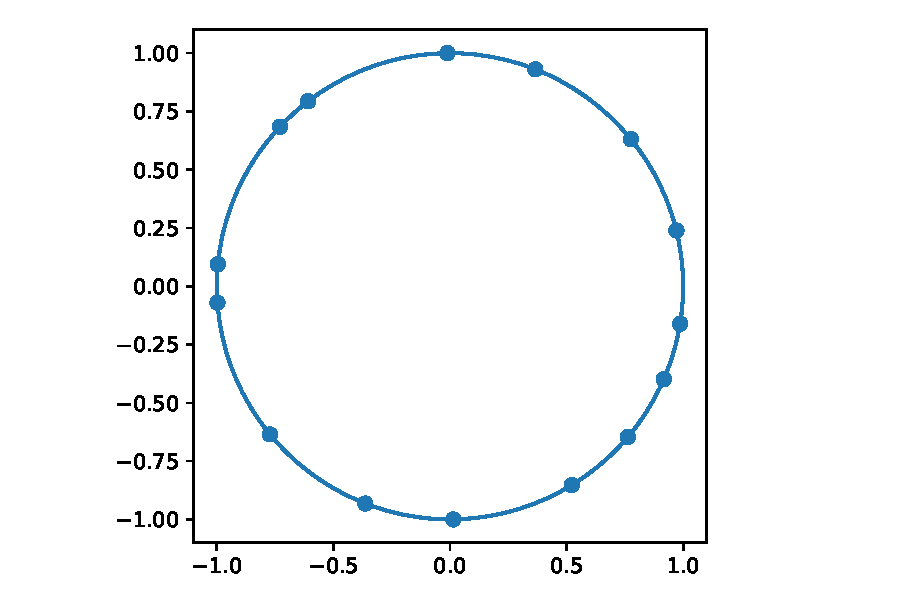
\includegraphics[width= 0.32\textwidth]{img/circle/CUE_design_N_15_fig_1.pdf}~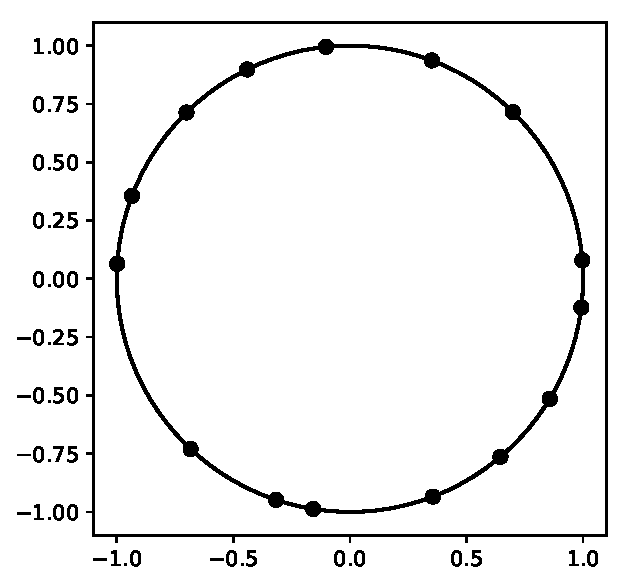
\includegraphics[width= 0.32\textwidth]{img/circle/CUE_design_N_15_fig_2.pdf}
~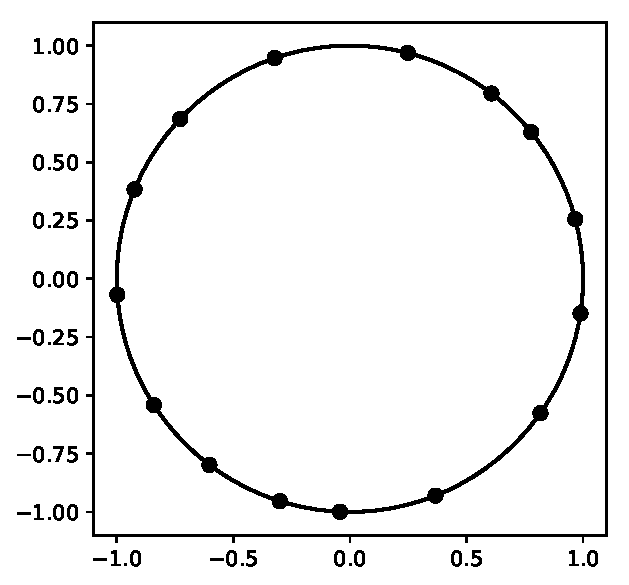
\includegraphics[width= 0.32\textwidth]{img/circle/CUE_design_N_15_fig_3.pdf}\\
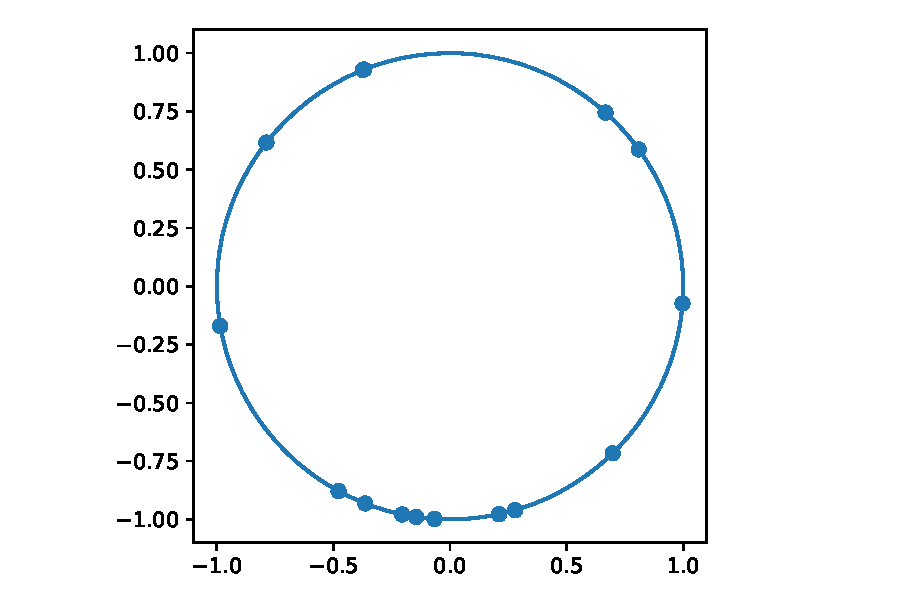
\includegraphics[width= 0.32\textwidth]{img/circle/iid_design_N_15_fig_1.pdf}~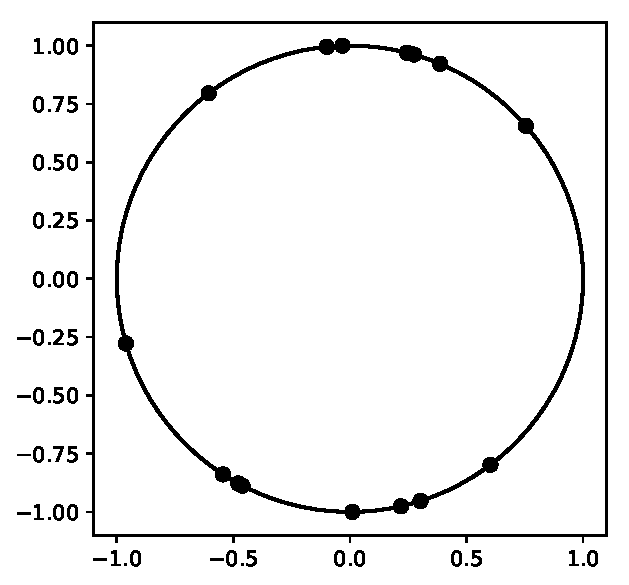
\includegraphics[width= 0.32\textwidth]{img/circle/iid_design_N_15_fig_2.pdf}
~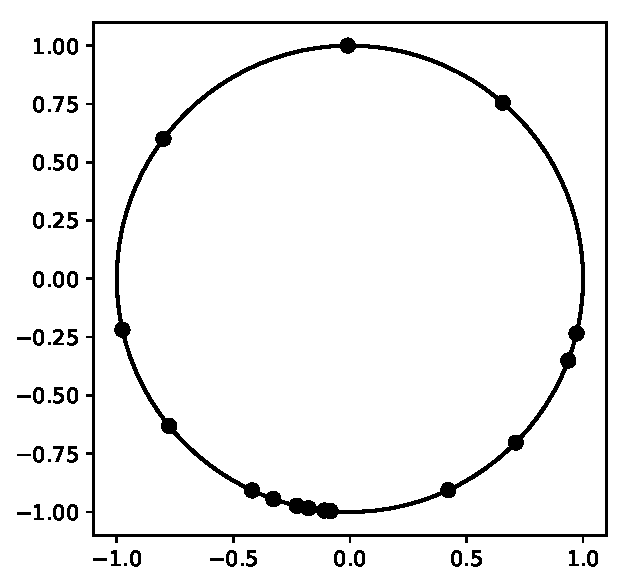
\includegraphics[width= 0.32\textwidth]{img/circle/iid_design_N_15_fig_3.pdf}\\
\caption{Three realizations from the CUE with $N = 15$ particles (top) compared to 15 particles sampled i.i.d in the unit circle (bottom). \label{fig:cue_vs_iid_particles}}
\end{figure}
 


% In other words, the joint distribution of the eigenvalues of a random unitary matrix with respect to Haar measure have the probability density:
% \begin{equation}\label{eq:haar_eigenvalues_density}
% \frac{1}{N!(2\pi)^{N}} \prod\limits_{1 \leq n,n' \leq N} |e^{-i \theta_{n}} - e^{-i \theta_{n'}}|^{2}
% \end{equation}
% on $\mathbb{U}^{N}$.







\paragraph{Ginibre ensemble}
\cite{Gin65} studied the statistical properties of the eigenvalues of matrices with independent Gaussian entries: real valued, complex valued and quaternion valued. These ensembles bear his name and follows the distribution of a DPP.
\begin{theorem}[\cite{Gin65}]
Let $M$ be an $N\times N$ matrix with i.i.d. standard complex Gaussian entries.
Then the eigenvalues of $M$ follows the distribution of the determinantal point
process associated to the kernel defined on the complex plan
\begin{equation}
\kappa(z,w) = \sum\limits_{\ell =0}^{N-1} \frac{(z \overline{w})^{\ell}}{\ell!},
\end{equation}
with respect to the reference measure $\mathrm{d}\omega(z) = \frac{1}{\pi}e^{-|z|^{2}} \mathrm{d}\lambda(z)$, where $\mathrm{d}\lambda$ is the Lebesgue measure on $\mathbb{C}$.
\end{theorem}




\begin{figure}
\centering
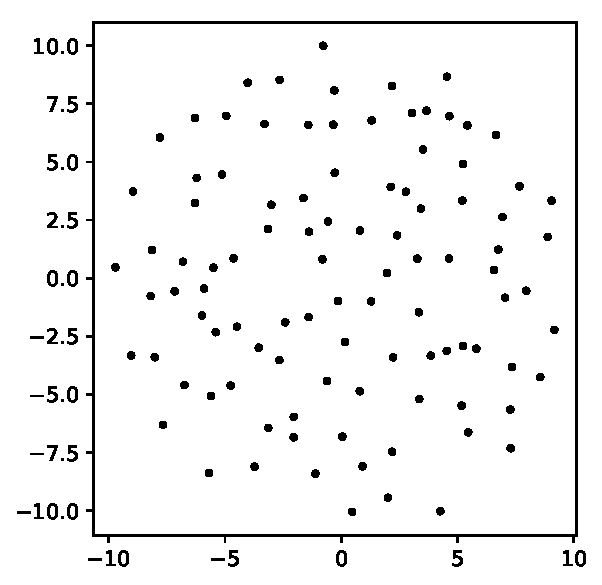
\includegraphics[width= 0.32\textwidth]{img/Ginibre/Ginibre_100_example_id_1.pdf}~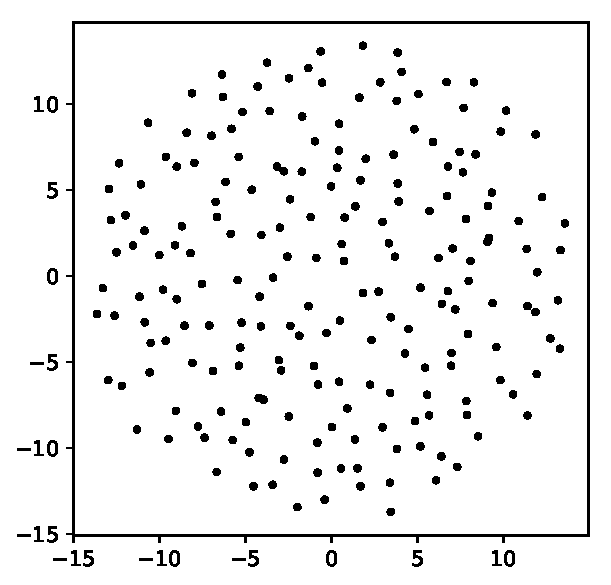
\includegraphics[width= 0.32\textwidth]{img/Ginibre/Ginibre_200_example_id_2.pdf}~
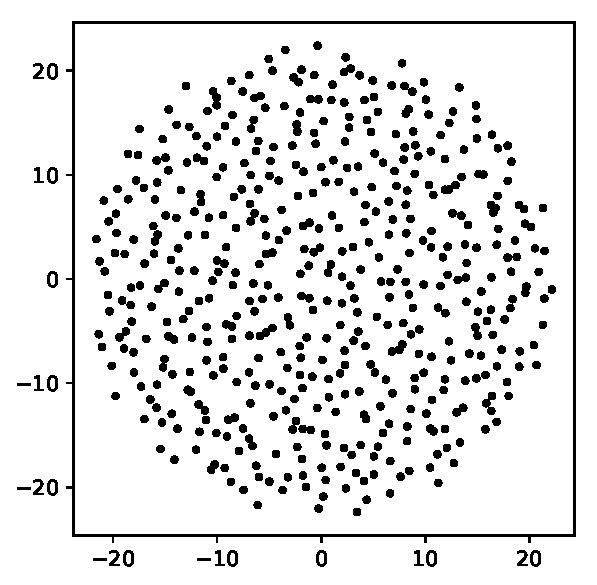
\includegraphics[width= 0.32\textwidth]{img/Ginibre/Ginibre_500_example_id_3.pdf}\\
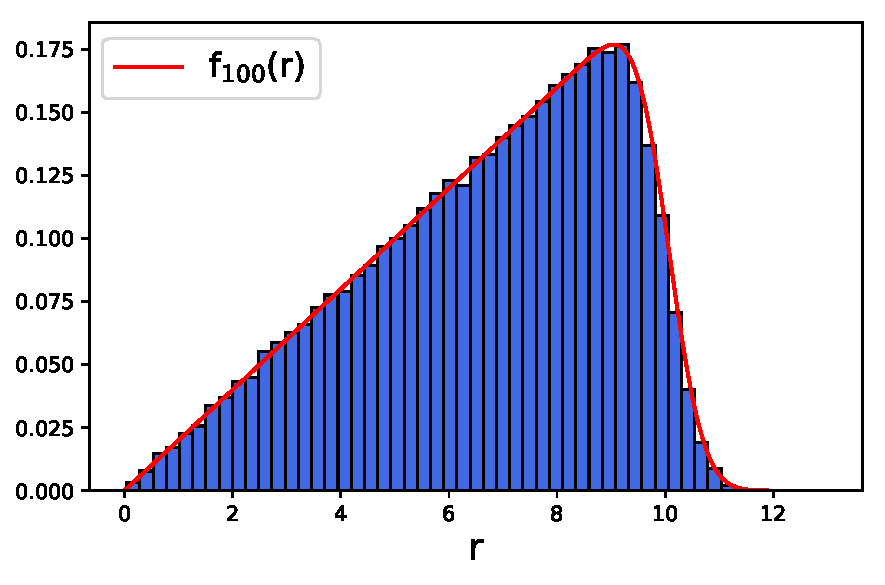
\includegraphics[width= 0.32\textwidth]{img/Ginibre/Ginibre_histogram_1000_N_100_example_2.pdf}~
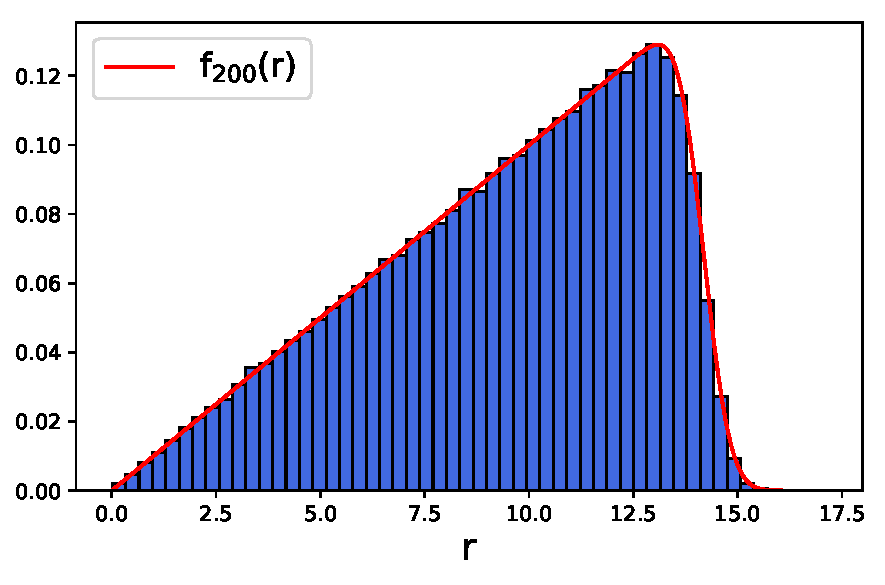
\includegraphics[width= 0.32\textwidth]{img/Ginibre/Ginibre_histogram_1000_N_200_example_2.pdf}~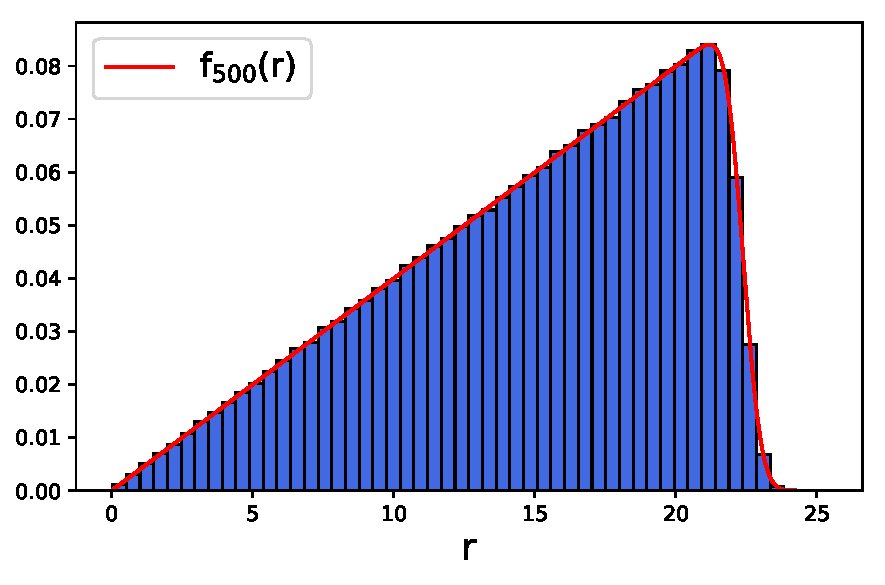
\includegraphics[width= 0.32\textwidth]{img/Ginibre/Ginibre_histogram_1000_N_500_example_2.pdf}
\caption{A realization of the Ginibre ensemble with $N = 100$ (left), $N = 200$ (middle) and $N = 500$ (right). The histogram of the radii $|z|$ of 1000 realization of the Ginibre ensemble compared to the theoretical density $f_{N}$, with $N = 100$ particles (left) $N = 200$ particles (middle) and $N = 500$ particles (right). \label{fig:ginibre}}
\end{figure}


% \begin{figure}
% \centering

% \caption{. \label{fig:ginibre_mean_measure}}
% \end{figure}


Observe that the kernel $\kappa$ defines a projection operator from $\mathbb{L}_{2}(\mathrm{d}\omega)$ onto the $N$ dimensional subspace spanned by the functions $z \mapsto z^{n}$; $n \in \{0, \dots, N-1 \}$. As $N \rightarrow +\infty$, the kernel $\kappa$ converges to the kernel
\begin{equation}
\kappa_{\infty}(z,w) = e^{z \overline{w}},
\end{equation} 
that defines the space
of all entire functions in $\mathbb{L}_{2}(\mathrm{d}\omega)$. 

The top of Figure~\ref{fig:ginibre} shows a  realization of three Ginibre ensembles corresdponding to $N \in \{100,200,500\}$. We observe that for the three values of $N$, the configuration takes a "spherical form" that can be explained by the rotational invariance of the mean measure $\kappa(z,z) \mathrm{d}\omega(z)$. Moreover, the modulus of the elements of the Genibre ensemble form a point process on $\mathbb{R}_{+}$, and the corresdponding mean measure have a density with respect to the Lebesgue measure that writes
\begin{equation}
f_{N}(r) = \frac{2}{N}\sum\limits_{\ell =0}^{N-1} \frac{r^{2\ell+1}}{\ell!}e^{-r^{2}} \mathbb{1}_{\mathbb{R}_{+}}(r).
\end{equation}

The bottom of the Figure~\ref{fig:ginibre} shows histograms of the modulus computed on 1000 samples of the Ginibre ensemble for the three values of $N \in \{100,200,500\}$  compared to the respective densities $f_{100},f_{200}$ and $f_{500}$. Besides the matching between the theoretical density $f_{N}$ and the empirical histogram observed for the three values of $N$; we observe that density $f_{N}$ is unimodal and achieves its maximal value at $r \approx \sqrt{N}$, then manifest a sharp drop to very small values.

% Figure~\ref{fig:ginibre_mean_measure} shows the histograms of the modulus calculated using 1000 realizations of the Ginibre ensemble with $N \in \{ 100,200,500\}$ compared to the corresponding densities $f_{100},f_{200},f_{500}$. 

 % compared to three realizations from the binomial process ($N = 15$) corresponding to the the Lebesgue measure on $\mathbb{U}$. We observe that the CUE tends to be cover the unit circle with more regularity than the binomial process.


\paragraph{The spherical enemble}
The spherical ensemble is another example of a DPP based on the eigenvalues of random matrices. This ensemble is defined on the complex plan; yet, using the inverse of the stereographic projection, it can be seen as a DPP on the sphere $\mathbb{S}^{2}$, hence the name. This ensemble was already used in theoretical physics for the modeling of repulsive particles in the sphere \citep{Cai81} \citep{FoJaMa92}. The spectral representation of this DPP was discovered by \cite{Kri09}. 



\begin{theorem}[Theorem 3 in \citep{Kri09}]\label{thm:spherical_ensemble}
Let $A,B$ be independent $N~\times~N$ matrix with i.i.d. standard complex Gaussian entries. The counting measure corresponding to the eigenvalues $\{z_{1}, \dots, z_{N}\} \subset \mathbb{C}$ of $A^{-1}B$ follows the distribution of the determinantal point
process associated to the kernel defined on the complex plan
\begin{equation}
\kappa_{\mathbb{C}}(z,w) = (1+z\overline{w})^{N-1},
\end{equation}
with respect to the reference measure $\mathrm{d}\omega(z) = \frac{N}{\pi(1+|z|^{2})^{N+1}} \mathrm{d}\lambda(z)$, where $\mathrm{d}\lambda$ is the Lebesgue measure on $\mathbb{C}$.

%  and 
\end{theorem}
Theorem~\ref{thm:spherical_ensemble} have can be reinterpreted as follows. 
Let $\pi: \mathbb{C} \cup \{ \infty \} \rightarrow \mathbb{S}^{2}$ be the inverse of the stereographic projection 
defined by
\begin{equation}
\pi(z) = \frac{1}{1+|z|^{2}} \Big(2\mathfrak{Re}(z), 2\mathfrak{Im}(z),|z|^{2}-1 \Big).
\end{equation}
For every $n \in [N]$ let $x_n = \pi(z_n)$. Then, $\{x_{1}, \dots, x_{N}\}$ follows the distribution of the determinantal point process associated to the kernel
 \begin{equation}
 \kappa_{\mathbb{S}^{2}}(x,y) = \kappa_{\mathbb{C}}(\pi^{-1}(x),\pi^{-1}(y)),
 \end{equation}
with respect to the uniform measure on $\mathbb{S}^{2}$.




\begin{figure}
\centering
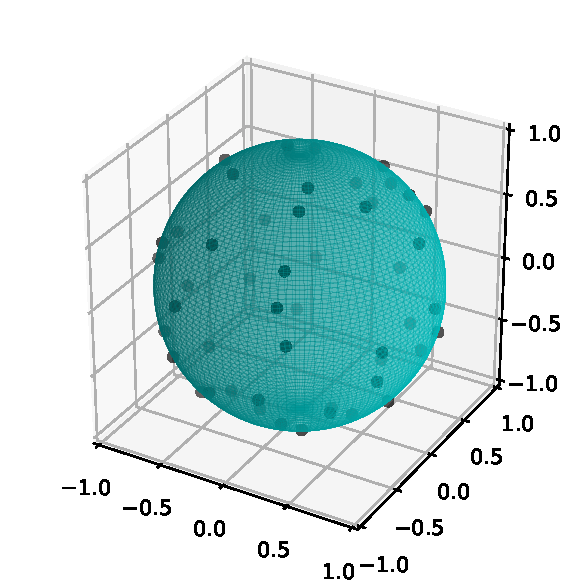
\includegraphics[width= 0.32\textwidth]{img/Spherical/Spherical_50_example_id_1.pdf}~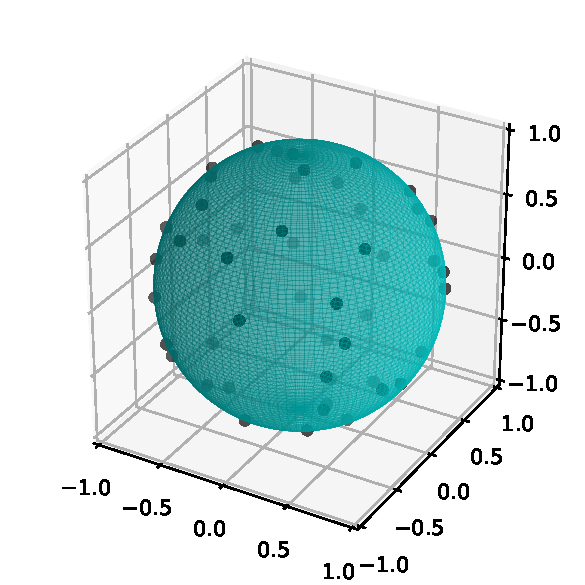
\includegraphics[width= 0.32\textwidth]{img/Spherical/Spherical_50_example_id_2.pdf}
~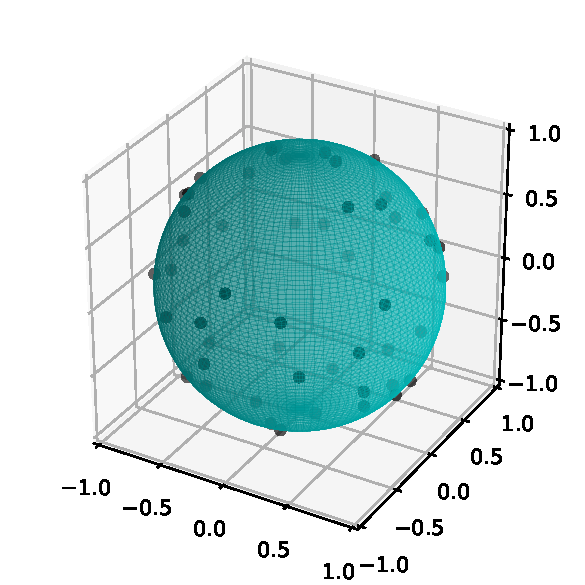
\includegraphics[width= 0.32\textwidth]{img/Spherical/Spherical_50_example_id_3.pdf}\\
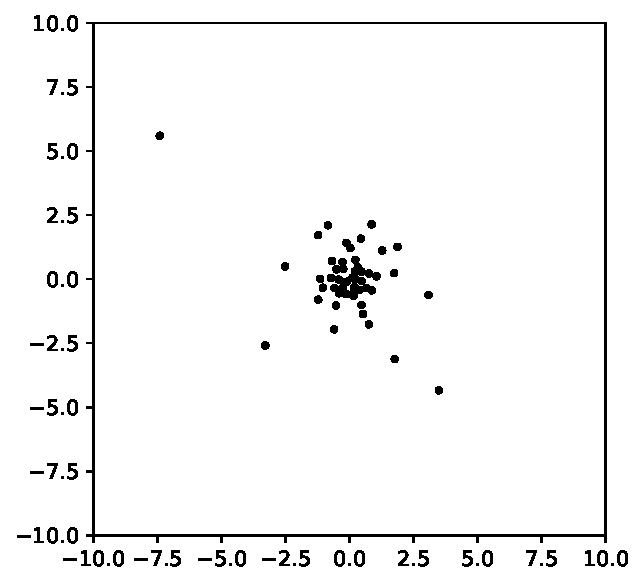
\includegraphics[width= 0.32\textwidth]{img/Spherical/Spherical_beforestero_50_example_id_1.pdf}~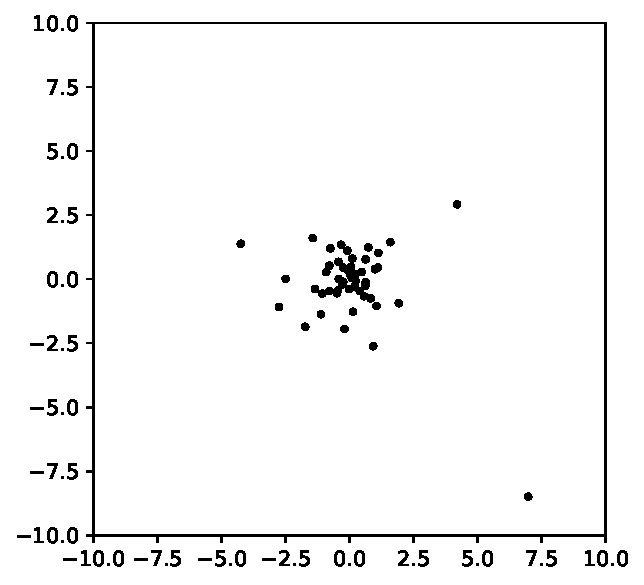
\includegraphics[width= 0.32\textwidth]{img/Spherical/Spherical_beforestero_50_example_id_2.pdf}
~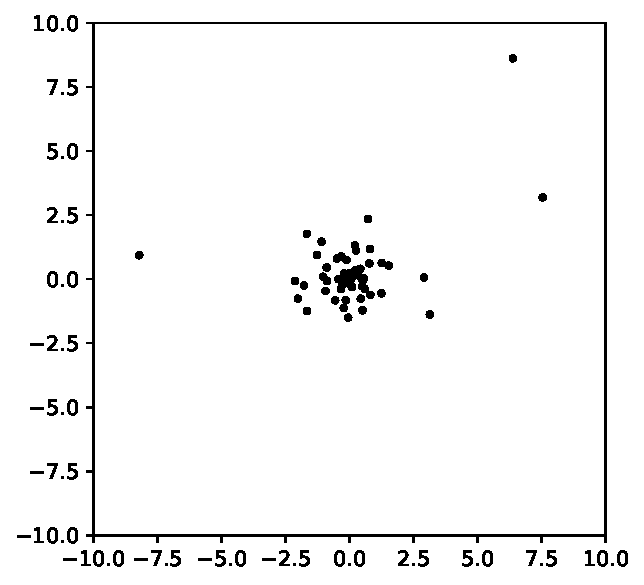
\includegraphics[width= 0.32\textwidth]{img/Spherical/Spherical_beforestero_50_example_id_3.pdf}\\
\caption{Three realizations from the spherical ensemble with $N = 50$ particles (top) compared to their stereographic projections on the complex plan (bottom). \label{fig:spherical_ensemble}}
\end{figure}

% \begin{theorem}[\cite{Gin65}]
% Let $M$ be an $N\times N$ matrix with i.i.d. standard complex Gaussian entries.
% Then the eigenvalues of $M$ follows the distribution of the determinantal point
% process associated to the kernel defined on the complex plan
% \begin{equation}
% \kappa(z,w) = \sum\limits_{\ell =0}^{N-1} \frac{(z \overline{w})^{\ell}}{\ell!},
% \end{equation}
% with respect to the reference measure $\mathrm{d}\omega(z) = \frac{1}{\pi}e^{-|z|^{2}} \mathrm{d}\lambda(z)$, where $\mathrm{d}\lambda$ is the Lebesgue measure on $\mathbb{C}$.
% \end{theorem}


\subsection{Numerical simulation}\label{sec:num_algos_dpps}
As we have seen in Theorem~\ref{minors_symmetric_polynomials_lemma}, DPPs that satisfies the usual  conditions \eqref{eq:hermitian_condition_kappa}, \eqref{eq:positivity_condition_kappa}, \eqref{eq:integrability_condition_kappa} and \eqref{eq:traceclass_condition_kappa} are mixtures of projection DPPs. This decomposability motivates the interest in simulating projection DPPs. We review in this section the literature on the numerical simulation of projection DPPs.

\subsubsection{Algorithms based on random matrix models}
% As we have seen in the introduction, the eigenvalues of a random unitary matrix ... 
As we have seen in Section~\ref{sec:DPP_examples}, the eigenvalues of some random matrix models corresponds to some specific projection DPPs. This is the case of the Circular Unitary Ensemble, the Ginibre Ensemble and the Spherical Ensemble. 

Orthogonal Polynomial Ensembles (OPE) on the real line form another class of projection DPPs that can be represented as the eigenvalues of some random matrix models. For this class of DPPs, the kernel $\kappa$ writes
\begin{equation}
\kappa(x,y) = \sum\limits_{n =0}^{N-1} P_{n}(x)P_{n}(y),
\end{equation}
where $(P_{n})$ is a family of orthonormal polynomials with respect to some measure $\mathrm{d}\omega$.

% are  Projection DPPs corresponding to 
In particular, when $\mathrm{d}\omega$ is a Gaussian, gamma \cite{DuEd02}, or beta \cite{KiNe04}, the corresponding DPP can be sampled by tridiagonalizing a matrix with independent entries with a cost that scales as $\mathcal{O}(N^2)$.
We illustrate this technique in Section~\ref{sec:Gaussian_quadrature} in Chapter~\ref{chap:dppkq}. We refer to \citep{GaBaVa20} for more details on this topic.

Now, in general, there exists an algorithm for the numerical simulation of a projection DPP. This algorithm will be recalled in the following section.
% and bypasses the need for rejection sampling. 





\subsubsection{The HKPV algorithm}
 
%  Recall that by Proposition~\ref{prop:projection_DPP_cardinality},  a projection DPP, of kernel $\kappa$ and reference measure $\mathrm{d}\omega$,  defines a random counting measure $\gamma$ with deterministic cardinality 
%  \begin{equation}
% \Prb \big( |\gamma| = N \big) = 1,
%  \end{equation}
%  % random set that follows the distribution of a projection DPP of marginal kernel $\KDPP$ have a deterministic cardinal equals to $N$, 
%  where $N$ is the rank of the integral operator associated to the kernel $\kappa$ and the measure $\mathrm{d}\omega
%  $. For this reason, we can identify such a random set with a sample from a random variable defined on $\mathcal{X}^{N}$.

% Let $\bm{x} = \{x_{1}, \dots, x_{N}\}$ a random set that follows the distribution of a projection DPP of marginal kernel $\KDPP_{N}$. The joint distribution of the random variable $(x_{1}, \dots, x_{N}) \in \X^{N}$ have a density with respect to the measure $\mathrm{d}\bm{\omega}(\bm{x}) = \otimes_{n\in [N]}\mathrm{d}\omega(x_{n})$:
% \begin{equation}\label{eq:det_density}
% f_{\KDPP}(\bm{x}) = \frac{1}{N!}\Det \bm{\KDPP}(\bm{x}).
% \end{equation}

% As we shall see, the landscape on this topic is 


% \begin{figure}[!ht]
%  \centerline{
%  \scalebox{0.9}{
% \begin{algorithm}{$\Algo{RME}\big(N)$}
% \Aitem $n \longleftarrow  N$
% \Aitem $\mu_{N}(x) \longleftarrow  \frac{1}{N} \KDPP(x,x)\mathrm{d}\omega(x)$
% \Aitem $\bm{x} \longleftarrow  \emptyset$
% \Aitem \While $n > 0 $
% \Aitem \mt $\mu_{n}(x) = \frac{1}{n} \left( \KDPP(x,x) - \KDPP(x,\bm{x})^{\Tran}\bm{\KDPP}(\bm{x})^{-1} \KDPP(x,\bm{x}) \right) \mathrm{d}\omega(x)$ \ar{Chain rule}
% \Aitem \mt  Pick $x_{n}$ from $\mathcal{X}$ from $\mu_{n}$ \ar{Sample from the conditional}
% \Aitem \mt  $\bm{x} \longleftarrow  \bm{x} \cup \{x_{n}\}$
% \Aitem \mt $n \longleftarrow  n-1$
% \Aitem \Return $\bm{x}$
% \end{algorithm}
%  }
%  }
% \caption{Pseudocode a sampler of projection DPP based on a random matrix model.}
% \label{alg:RME_SAMPLER}
% \end{figure}


%\paragraph{The sequential algorithm HKPV}
Consider $(\psi_{m})_{m \in [N]}$ an orthonormal family with respect to the measure $\mathrm{d}\omega$. In \citep*{HoKrPeVi06}, a sequential algorithm was proposed for the numerical simulation of a random set that follows the distribution of the projection DPP of  kernel
\begin{equation}
\kappa(x,y) = \sum\limits_{m \in [N]} \psi_{m}(x)\psi_{m}(y).
\end{equation}

Recall that by Proposition~\ref{prop:projection_DPP_cardinality} the cardinality of this random set is deterministic  
 \begin{equation}
\Prb \big( |\gamma| = N \big) = 1,
 \end{equation}
%  % random set that follows the distribution of a projection DPP of marginal kernel $\KDPP$ have a deterministic cardinal equals to $N$, 
%  where $N$ is the rank of the integral operator associated to the kernel $\kappa$ and the measure $\mathrm{d}\omega
For this reason, we can identify such a random set with a sample from a random variable defined on $\mathcal{D}^{N}$.
 
Indeed, the idea behind this algorithm is to see $\bm{\kappa}(\bm{x})$ as the Gram matrix of the family $\big(\kappa(x_{n},.)\big)_{n \in [N]}$, whose $i,j$ entry is given by the scalar product of $\kappa(x_{i},.)$ and $\kappa(x_{j},.)$ with respect to the scalar product defined by $\mathrm{d}\omega$. In fact, by the orthonormality of $(\psi_{m})_{m \in [N]}$
%\int_{\mathcal{X}} \kappa(x_{i},x) \kappa(x_{j},x) \mathrm{d}\omega(x)
\begin{equation}
\Big\langle \kappa(x_{i},.),\kappa(x_{j},.) \Big\rangle_{\mathrm{d}\omega}  = \sum\limits_{m \in [N]}\sum\limits_{m' \in [N]} \int_{\mathcal{X}} \psi_{m}(x_{i}) \psi_{m}(x) \psi_{m'}(x_{j}) \psi_{m'}(x) \mathrm{d}\omega(x)  = \kappa(x_{i},x_{j}).
\end{equation}

Hence, $\Det \bm{\kappa}(\bm{x})$ corresponds to the volume of the parallelepiped defined in $\mathbb{L}_{2}(\mathrm{d}\omega)$ and spanned by the vectors $(\kappa(x_{n},.))_{n \in [N]}$. Using base$\times$height formula, the authors proved that the density, with respect to the measure $\mathrm{d}\bm{\omega}(\bm{x}) = \otimes_{n\in [N]}\mathrm{d}\omega(x_{n})$,
\begin{equation}\label{eq:det_density}
f_{\KDPP}(\bm{x}) = \frac{1}{N!}\Det \bm{\kappa}(\bm{x})
\end{equation}
factorizes as the product of $N$ densities (with respect to $\mathrm{d}\omega$)
\begin{equation}
f_{\kappa}(x_{1},\dots,x_{N}) = \prod\limits_{n \in [N]} f_{\kappa,n}(x_{n}),
\end{equation}
where
% for every $n \in [N]$ the conditional expresses as
\begin{equation}
f_{\kappa,1}(x) = \frac{1}{N} \kappa(x,x),
\end{equation}
and for $n>1$
\begin{equation}
f_{\kappa,n}(x) = \frac{1}{N-n+1} \left( \kappa(x,x) - \kappa(x,\bm{x}_n)^{\Tran}\bm{\kappa}(\bm{x}_n)^{-1} \kappa(x,\bm{x}_n) \right),
\end{equation}
where $\bm{x}_{n} = (x_1,x_2, \dots, x_{n-1} )$ and $\kappa(x,\bm{x}_n) = (\kappa(x,x_{\ell}))_{\ell \in [n]}$. In particular, the Algorithm~\ref{alg:HKPV_SAMPLER} outputs a random set that can be identified with a random counting measure that follows the distribution of the projection DPP of marginal kernel $\kappa$ and reference measure $\mathrm{d}\omega$.



\begin{figure}[!ht]
 \centerline{
 \scalebox{0.9}{
\begin{algorithm}{$\Algo{HKPV}\big(\kappa(x,y), \mathrm{d}\omega \big)$}
\Aitem $n \longleftarrow  N$
\Aitem $\mu(x) \longleftarrow  f_{\kappa,1}(x) \mathrm{d}\omega(x)$ \ar{Initialize the distribution}
\Aitem $\bm{x} \longleftarrow  \emptyset$
\Aitem \While $n > 0 $
\Aitem \mt  Pick $x_{N-n+1}$ in $\mathcal{D}$ from $\mu$ \ar{Sample from the distribution}
\Aitem \mt  $\bm{x} \longleftarrow  \bm{x} \cup \{x_{N-n+1}\}$
\Aitem \mt $n \longleftarrow  n-1$
\Aitem \mt $\mu(x) \longleftarrow f_{\kappa,n}(x) \mathrm{d}\omega(x)$ \ar{Update the distribution}
\Aitem \Return $\bm{x}$
\end{algorithm}
 }
 }
\caption{Pseudocode of the HKPV algorithm for sampling from a projection DPP of marginal kernel $\kappa$.}
\label{alg:HKPV_SAMPLER}
\end{figure}
 In practice, the implementation of this algorithm requires to sample from the conditional distributions $f_{\kappa,n}\mathrm{d}\omega$ (Step 5 in Algorithm~\ref{alg:HKPV_SAMPLER}). An implementation of this step was proposed in \citep{BaHa16} based on the following observation 
 \begin{equation}
f_{\kappa,n}(x) \leq \frac{N}{n}f_{\kappa,1}(x) = \frac{N}{n} \kappa(x,x).
 \end{equation} 

Therefore, it is enough to sample from the first distribution $f_{\kappa,1} \mathrm{d}\omega$ and use rejection sampling for the other conditionals.

We give an illustration of this algorithm in two cases: i) $\psi_{m}$ are the normalized Legendre polynomials defined on $\mathcal{D}= [-1,1]$, ii) $\psi_m$ are the Haar wavelets defined on $\mathcal{D}= [0,1]^{2}$.

% We consider 
% In the first case, recall that the normalized Legendre polynomials are defined by 


% we use the following upper bound on  

% \paragraph{The HKPV algorithm for the normalized Legendre polynomials}
% In fact, in many situations 

%  This is the case when the $(\psi_{n})$ is a family of orthogonal polynomials and $\mathcal{X} = [0,1]^{d}$.  

%\clearpage
\chapter{The column subset selection problem}\label{chapter:cssp}
\section{Introduction}

%!TEX root=./submitted.tex

%\section{Introduction}

Datasets come in always larger dimensions, and dimension reduction is thus often one the first steps in any machine learning pipeline. Two of the most widespread strategies are principal component analysis (PCA) and feature selection. PCA projects the data in directions of large variance, called principal components. While the initial features (the canonical coordinates) generally have a direct interpretation, principal components are linear combinations of these original variables, which makes them hard to interpret. On the contrary, using a selection of original features will preserve interpretability when it is desirable. Once the data are gathered in an $N\times d$ matrix, of which each row is an observation encoded by $d$ features, feature selection boils down to selecting columns of $\bm{X}$. Independently of what comes after feature selection in the machine learning pipeline, a common performance criterion for feature selection is the approximation error in some norm, that is, the norm of the residual after projecting $\bm{X}$ onto the subspace spanned by the selected columns. Optimizing such a criterion over subsets of $\{1,\dots,d\}$ requires exhaustive enumeration of all possible subsets, which is prohibitive in high dimension. One alternative is to use a polynomial-cost, random subset selection strategy that favours small values of the criterion.
%

This rationale corresponds to a rich literature on randomized algorithms for column subset selection \citep{DeVe06,DrMaMu07,BoDrMI11}. A prototypal example corresponds to sampling $s$ columns of $\bm{X}$ i.i.d. from a multinomial distribution of parameter $\bm{p} \in \mathbb{R}^{d}$. This parameter $\bm{p}$ can be the squared norms of each column \citep{DFKVV04}, for instance, or the more subtle $k$-leverage scores \citep{DrMaMu07}. While the former only takes $\mathcal{O}(d N)$ time to evaluate, it comes with loose guarantees; see Section~\ref{subsec:length_square_sampling}. The $k$-leverage scores are more expensive to evaluate, since they call for a truncated SVD of order $k$, but they come with tight bounds on the ratio of their expected approximation error over that of PCA.

% diversity for large subsapace with few features
To minimize approximation error, the subspace spanned by the selected columns should be as large as possible. Simultaneously, the number of selected columns should be as small as possible, so that intuitively, diversity among the selected columns is desirable. The column subset selection problem (CSSP) then becomes a question of designing a discrete point process over the column indices $\{1,\dots,d\}$ that favours diversity in terms of directions covered by the corresponding columns of $\bm{X}$.
% bounds are necessary
Beyond the problem of designing such a point process, guarantees on the resulting approximation error are desirable. Since, given a target dimension $k\leq d$ after projection, PCA provides the best approximation in Frobenius or spectral norm, it is often used as a reference: a good CSS algorithm preserves interpretability of the $c$ selected features while guaranteeing an approximation error not much worse than that of rank-$k$ PCA, all of this with $c$ not much larger than $k$.
% For example, in \cite{DFKVV04} the authors proved additive approximation bound while \citep{DrMaMu07} proved relative approxi, \citep{BoDrMI11}, \citep{DeVe06} and \citep{PaKyBo14}
% Types of bounds
 % \pc{Peut-être plus tard avec les équations ? mais au moins dire qu'il existe des résultats dans la littérature en quelques phrases, en renvoyant à la bonne seciton pour plus de détails : message = c'est un pb intéressant et on va faire mieux que les autres !}
 % {\bf Here explain the type of bounds : in high proba, additive, multiplicative, but with words.}
 % In the literature ... bounds in expectation on the approximation error with high probability...

% Nous
In this paper, we introduce and analyse a new randomized algorithm for selecting $k$ diverse columns. Diversity is ensured using a determinantal point process (DPP). DPPs can be viewed as the kernel machine of point processes; they were introduced by \cite{Mac75} in quantum optics, and their use widely spread after the 2000s in random matrix theory \citep{Joh05}, machine learning \citep{KuTa12}, spatial statistics \citep{LaMoRu15}, and Monte Carlo methods \citep{BaHa16}, among others. In a sense, the DPP we propose is a nonindependent generalization of the multinomial sampling with $k$-leverage scores of \cite{BoMaDr09}. It further naturally connects to volume sampling, the CSS algorithm that has the best error bounds \citep{DRVW06}. We give error bounds for DPP sampling that exploit sparsity and decay properties of the $k$-leverage scores, and outperform volume sampling when these properties hold. Our claim is backed up by experiments on toy and real datasets.

%%%%
%{\bf Beginning of old version}
%%%%
%Principal Component Analysis (PCA) is a widely used technique for dimension reduction applied on datasets in all scientific domains. This method consists in projecting the data in directions of large variances called principal directions. In many applications, the initial factors (the canonical coordinates) have a direct physical interpretation. For example in financial, biological or text analysis applications, each axis might correspond to a specific asset, gene or word. Hence, it is natural to seek to calculate factors capturing the most of the data variance using few coordinate variables. In general, the factors given by the PCA are linear combinations of all original variables. This property could hinder the interpretation of these new artificial factors. To address this limitation, we consider the problem of dimension reduction using the initial factors, this boils down to the selection a subset of columns, corresponding to a subset of features that represents the initial matrix. In particular, we consider the problem of selecting exactly $k$ columns from a matrix $\bm{X} \in \mathbb{R}^{N \times d}$ gathered in a submatrix $\bm{C}$: these $k$ features are actual features from the data as opposed to the $k$ eigenvectors returned by the Principal Component Analysis that are linear combinations of all the $d$ features. Formally, we look to select the subset of $k$ columns of $\bm{X}$ that captures as much as possible of the variance in $\bm{X}$ in the following sense:
%\begin{problem}
%\label{d:xxx}
%Let $\bm{X} \in \mathbb{R}^{N \times d}$ and $k$ a positive integer. Pick $k$ columns of $\bm{X}$ called $\bm{C} \in \mathbb{R}^{N \times k}$ such that the residual
%\begin{equation}
%    \| \bm{X} - \Pi_{C}\bm{X}\|_{\nu}
%\end{equation}
%is minimized over all possible ${d}\choose{k}$ choices for the matrix $\bm{C}$, where $\|.\|_{\nu}$ is the spectral norm or the Frobenius norm, and $\Pi_{C} = \bm{C}\bm{C}^{+} \in \mathbb{R}^{N \times N}$ \rb{Attention, si la projection dépend de la norme, il faut le dire} is the projection onto the $k$-dimensional space spanned by the columns of $\bm{C}$.
%\end{problem}
%%The output of a CSSP algorithm would be a subset of $k$ features represented by a matrix $\bm{C}~\in~\mathbb{R}^{N \times k}$. and many algorithms were proposed to approximate the exact solution
%This is a combinatorial optimization problem for which we can define a relaxation
%as following: pick a subset of $k$ columns of $\bm{X}$ called $\bm{C}$ such that there exist $\gamma \geq 1$ such that
%% Principal Component Analysis (PCA) is a widely used technique for dimension reduction. This method consist in projecting the data in directions of large variances called principal directions. This algorithm was first studied by Pearson \citep{Pea01} and Hotelling \citep{Hot33}. In this note, we investigate the problem of selecting exactly k columns from an $N \times d$ $\bm{X}$ matrix. The aim of such an optimization problem is to select the subset of $k$ columns of $\bm{X}$ that captures as much as possible of $\bm{X}$ in the following sense:
%% \begin{definition}
%% \label{d:xxx}
%% Let $\bm{X} \in \bm{R}^{N \times d}$ and $k$ a positive integer. Pick $k$ columns of $\bm{X}$ called $\bm{C} \in {N \times k}$ such that the residual
%% \begin{equation}
%%     \| \bm{X} - \Pi_{C}\bm{X}\|_{Fr}
%% \end{equation}
%% is minimized over all possible ${d}\choose{k}$ choices for the matrix $\bm{C}$, where $\Pi_{C} = \bm{C}\bm{C}^{+} \in \bm{R}^{N}$ is the projection onto the $k$-dimensional space spanned by the columns of $\bm{C}$.
%% \end{definition}
%
%% The main application of the CSSP is features selection \citep{BoMaDr08}. Consider for example $\bm{X} \in \mathbb{R}^{N \times d}$ a matrix representing $N$ objects with $d$ features, the output of a CSSP algorithm would be a subset of $k$ features represented by a matrix $\bm{C} \in \mathbb{R}^{N \times k}$. These $k$ features are actual features from the data as opposed to the $k$ eigenvectors returned by the Principal Component Analysis that are linear combinations of all the $d$ features.
%\begin{equation}
%    \| \bm{X} - \Pi_{k}\bm{X}\|_{\nu} \leq \| \bm{X} - \Pi_{C}\bm{X}\|_{\nu} \leq \gamma \| \bm{X} - \Pi_{k}\bm{X}\|_{\nu}.
%\end{equation}
%
%
%Note that while we focus on the problem of selecting exactly $k$ columns from $\bm{X}$, another possible relaxation of the CSSP problem was studied in the literature \citep{DrMaMu07}, \citep{BoDrMI11}, \citep{DeVe06} and \citep{PaKyBo14}: pick a subset of $c$ columns (with $c >k$) of $\bm{X}$ called $\bm{C}$ such that
%\begin{equation}
%    \| \bm{X} - \Pi_{k}\bm{X}\|_{\nu} \leq \| \bm{X} - \Pi_{\bm{C},k}^{\nu}\bm{X}\|_{\nu} \leq f(k,d) \| \bm{X} - \Pi_{k}\bm{X}\|_{\nu}
%\end{equation}
%where $\Pi_{\bm{C},k}^{\nu}\bm{X}$ is the best approximation, in the sense of the norm $\|.\|_{\nu}$, of $\bm{X}$ within the column space of $\bm{C}=\bm{X}_{:,S}$ that has a rank at most $k$.
%
%Note that every selected column $\bm{X}_{:,i} \in \bm{C}$ corresponds an integer $i \in [d]$. Thus, picking columns from a matrix, corresponds to choosing indices $i \in [d]$ according to a selection algorithm.
%\begin{definition}
%A selection algorithm $\mathcal{A}: \bm{X} \mapsto \bm{C}$ can be
%defined using a point process $\mathcal{P}$ on $[d]$: a probability measure over subsets of $[d]$.
%\end{definition}
%In other words, a point process is a random subset of $[d]$. This definition encompasses deterministic selection algorithms. In deed, in this case the probability measure is reduced to a Dirac charging one subset of $[d]$. We call  call a non deterministic selection algorithm a randomized selection algorithm. The quality of the selection algorithm $\mathcal{A}$ can be assessed using the expected value of $\| \bm{X} - \Pi_{C}\bm{X}\|_{\nu}$ under the law of the point process $\mathcal{P}$
%\begin{equation}\label{eq:selection_algorithm_expected_bound}
%    \EX_{S \sim \mathcal{P}} \| \bm{X} - \Pi_{C}\bm{X}\|_{\nu} \leq f(k,d) \| \bm{X} - \Pi_{k}\bm{X}\|_{\nu}.
%\end{equation}
%Research on this question have been focused on designing selection algorithms with the lowest possible value of $f(k,d)$. Note that once we have an inequality of the type \eqref{eq:selection_algorithm_expected_bound}, a question of interest would be whether we can prove inequalities of the form
%\begin{equation}\label{eq:selection_algorithm_probabilistic_bound}
%    \Prb_{S \sim \mathcal{P}}(\| \bm{X} - \Pi_{C}\bm{X}\|_{\nu} \leq g(k,d,\delta) \| \bm{X} - \Pi_{k}\bm{X}\|_{\nu}) \geq 1-\delta.
%\end{equation}
%An important example of a randomized selection algorithm is based on sampling $s$ columns of $\bm{X}$ i.i.d from a multinomial distribution of parameter $\bm{p} \in \mathbb{R}^{d}$. This parameter can be equal to the length-squares distribution \cite{DFKVV04} or the more subtle $k$-leverage scores distribution \cite{DrMaMu07}. While the first distribution is cheap to evaluate (complexity in the order $\mathcal{O}(d N^{2})$), it comes with loose guarantees as reviewed in Section~\ref{subsec:length_square_sampling}. In the other hand, the $k$-leverage scores is more expensive to evaluate, since it involves a truncated SVD at order $k$, however it comes with multiplicative approximation bounds: for $\epsilon > 0$ and using $s = \mathcal{O}(\frac{k}{\epsilon^{2}})$ we achieve $g(k,d,\delta) = 1+\epsilon$ in \eqref{eq:selection_algorithm_probabilistic_bound}; we achieve almost optimal approximation bounds if we select sufficiently large number of columns.
%
%We present a new randomized algorithm for the problem of $k$-CSSP such that the $k$ columns selected are as diverse as possible. This randomized diversity could be expressed naturally using Determinantal Point Processes (DPPs). These models were introduced by Macchi \citep{Mac75} in quantum physics and their use spread: random matrix theory \citep{Joh05}, machine learning \citep{KuTa12} and Monte Carlo methods \citep{BaHa16}. We can define a DPP on $[d]$ using a positive semi-definite matrix $\bm{K}~\in~\mathbb{R}^{d\times d}$.
%\begin{definition}[DPP]
%A random subset $X \subset [d]$ is drawn from a DPP of marginal kernel $\bm{K}$ if and only if
%\begin{equation}\label{eq:def_dpp}
%\forall S \subset [d],\quad \Prb(S \subset X) = \Det(\bm{K}_{S}),
%\end{equation}
%where $\bm{K}_{S} = [\bm{K}_{(i,j)}]_{(i,j) \in S^{2}}$.
%\end{definition}


% \begin{definition}

% Let $\bm{X} \in \bm{R}^{N \times d}$ and $k$ a positive integer. Pick $c$ columns of $\bm{X}$ called $\bm{C} \in {N \times c}$. We note $\Pi_{\bm{C},k}^{\nu}\bm{X}$ the matrix of rank $k$ living in the column space of $\bm{C}$ minimizing  the residual
% \begin{equation}
%     \| \bm{X} - \Pi_{\bm{C},k}^{\nu}\bm{X}\|_{\nu}
% \end{equation}
% is minimized over all possible ${d}\choose{c}$ choices for the matrix $\bm{C}$, where $\Pi_{C} = \bm{C}\bm{C}^{+} \in \bm{R}^{N}$ is the projection onto the $k$-dimensional space spanned by the columns of $\bm{C}$.
% \end{definition}
%\subsection{Contributions}

% \begin{figure}[!ht]
% \centerline{
% \scalebox{0.9}{
% \begin{algorithm}{$\Algo{DPP}\big(\bm{X})$}
% %\vspace{-.1cm}
% \Aitem $(\bm{U},\bm{\Sigma},\bm{V}) \longleftarrow \text{SVD}(\bm{X})$
% \Aitem $Y \longleftarrow  \emptyset$
% \Aitem $s\bm{V} \longleftarrow  \bm{V}_{:,[k]}$
% \Aitem \While $\text{rk}(s\bm{V}) > 0 $
% \Aitem \mt  Sample $i$ from $\Omega$ with probability $\Prb(i) \propto \|s\bm{V}_{i,:}\|_{2}^{2}$
% \Aitem \mt  $Y \longleftarrow  Y \cup \{i\}$
% \Aitem \mt $s\bm{V} \longleftarrow s\bm{V}_{\perp}$ an orthonormal basis of $\Span(s\bm{V} \cap \bm{e}_{i}^{\perp})$
% \Aitem \Return $Y$
% \end{algorithm}
% }
% }
% \caption{Pseudocode of our randomized selection algorithm.}
% \label{alg:OUR_ALGO}
% \end{figure}
% The theoretical bounds proved for our algorithm depends on the . These bounds were validated using numerical simulations on toy datasets generated using a new algorithm described in Appendix~\ref{app:framebuilding}.


%\subsection{Outline of the paper}
The paper is organized as follows. Section~\ref{s:notation} introduces our notations. Section~\ref{s:relatedwork} is a survey of column subset selection, up to the state of the art to which we later compare. In Section~\ref{s:dppsection}, we discuss determinantal point processes and their connection to volume sampling. Section~\ref{sec:main_results} contains our main results, in the form of both classical bounds on the approximation error and risk bounds when CSS is a prelude to linear regression. In Section~\ref{s:numexpesection}, we numerically compare CSS algorithms, using in particular a routine that samples random matrices with prescribed $k$-leverage scores.

%%%%%%%%%%%
\section{Notation}
\label{s:notation}
We use $[n]$ to denote the set $\{1,\dots,n\}$, and $[n:m]$ for $\{n,\dots,m\}$. We use bold capitals $\bm{A},\bm{X},\dots$ to denote matrices. For a matrix $\bm{A} \in \mathbb{R}^{m \times n}$ and subsets of indices $I\subset[m]$ and $J\subset[n]$, we denote by $\bm{A}_{I,J}$ the submatrix of $\bm{A}$ obtained by keeping only the rows indexed by $I$ and the columns indexed by $J$. When we mean to take all rows or $\bm{A}$, we write $\bm A_{:,J}$, and similarly for all columns. We write $\rk (\bm{A})$ for the rank of $\bm{A}$, and $\sigma_i(\bm A)$, $i=1,\dots,\rk(\bm{A})$ for its singular values, ordered decreasingly. Sometimes, we will need the vectors $\Sigma(\bm{A})$ and $\Sigma(\bm{A})^2$ with respective entries $\sigma_i(\bm{A})$ and $\sigma_i^2(\bm{A})$, $i=1,\dots,\rk(\bm{A})$. Similarly, when $\bm{A}$ can be diagonalized, $\Lambda(\bm{A})$ (and $\Lambda(\bm{A})^2$) are vectors with the decreasing eigenvalues (squared eigenvalues) of $\bm{A}$ as entries. If $\bm{A}$ is a symmetric matrix, $\Sp(\bm{A})$ denotes the vector of its eigenvalues in decreasing order.

The spectral norm of $\bm{A}$ is $\|\bm{A}\|_{2} = \sigma_{1}(\bm A)$, while the Frobenius norm of $\bm{A}$ is defined by
$$\Vert\bm{A}\Vert_{\Fr} = \sqrt{\sum_{i=1}^{\rk(\bm{A})} \sigma_{i}(\bm{A})^{2}}.$$
For $\ell \in \mathbb{N}$, we need to introduce the $\ell$-th elementary symmetric polynomial on $L \in \mathbb{N}$ variables, that is
\begin{equation}
e_{\ell}(X_{1}, \dots, X_{L}) = \sum\limits_{\substack{T \subset [L]\\|T| = \ell}}~ \prod\limits_{j \in T} X_{j}.
\end{equation}
Finally, we follow \cite{Ben92} and denote spanned volumes by
$$\Vol_{q}(\bm{A}) = \sqrt{e_{q}\left(\sigma_{1}(\bm{A})^{2},\dots,\sigma_{\rk(A)}(\bm{A})^2\right)}, \quad q=1,\dots,\rk(\bm{A}).$$

Throughout the paper, $\bm{X}$ will always denote an $N\times d$ matrix that we think of as the original data matrix, of which we want to select $k\leq d$ columns. \rev{We do not make any assumption on how $N$ compares to $d$.} Unless otherwise specified, $r$ is the rank of $\bm{X}$, and matrices $\bm{U},\bm{\Sigma}$,$\bm{V}$ are reserved for the SVD of $\bm{X}$, that is,
\begin{align}
   \bm{X} &= \bm{U}\bm{\Sigma}\bm{V}^{\Tran}\\
   &=
\left[
\begin{array}{c|c}
\bm{U}_{k} & \bm{U}_{k^{\perp}}
\end{array}
\right]
\left[
\begin{array}{c|c}
\bm{\Sigma}_{k} & \bm{0} \\
\hline
\bm{0} & \bm{\Sigma}_{k^{\perp}}
\end{array}
\right]
\left[
\begin{array}{c}
\bm{V}_{k}^{\Tran} \\
\hline
\bm{V}_{k^{\perp}}^{\Tran}
\end{array}
\right],
\label{e:blockSVD}
\end{align}
where $\bm{U} \in \mathbb{R}^{N\times d}$ and $\bm{V} \in \mathbb{R}^{d \times d}$ are orthogonal, and $\bm{\Sigma} \in \mathbb{R}^{d \times d}$ is diagonal. The diagonal entries of $\bm{\Sigma}$ are $\sigma_i=\sigma_i(\bm{X})$, $i=1,\dots,r$, and we still assume they are in decreasing order. We will also need the blocks given in \eqref{e:blockSVD}, where we separate blocks of size $k$ corresponding to the largest $k$ singular values. To simplify notation, we abusively write $\bm{U}_{k}$ for $\bm{U}_{:,[k]}$ and $\bm{V}_{k}$ for $\bm{V}_{:,[k]}$ in \eqref{e:blockSVD}, among others. Though they will be introduced and discussed at length in Section~\ref{subsec:k-lvs_sampling}, we also recall here that we denote by $\ell_{i}^{k} = \|\bm{V}_{i,[k]}\|_{2}^{2}$ the so-called \emph{ $k$-leverage score} of the $i$-th column of $\bm{X}$.

We need some notation for the selection of columns. Let $S \subset [d]$ be such that $\vert S\vert =k$, and let $\bm{S} \in \{0,1\}^{d \times k}$ be the corresponding sampling matrix: $\bm{S}$ is defined by $\forall \bm{M} \in \mathbb{R}^{N\times d}, \bm{M}\bm{S} = \bm{M}_{:,S}$. In the context of column selection, it is often referred to $\bm{X}\bm{S} = \bm{X}_{:,S}$ as $\bm{C}$. We set for convenience $\bm{Y}_{:,S}^{\Tran} = (\bm{Y}_{:,S})^{\Tran}$.

The result of column subset selection will usually be compared to the result of PCA. We denote by $\Pi_k\bm{X}$ the best rank-$k$ approximation to $\bm{X}$. The sense of \emph{best} can be understood either in Frobenius or spectral norm, as both give the same result. On the other side, for a given subset $S \subset [d]$ of size $\vert S\vert=s$ and $\nu\in\{2,\Fr\}$, let
$$\Pi_{S,k}^{\nu}\bm{X} = \arg\min_{A} \Vert \bm{X}- A\Vert_{\nu}$$
where the minimum is taken over all matrices $\bm{A} = \bm{X}_{:,S}\bm{B}$ such that $\bm{B}\in\mathbb{R}^{s\times d}$ and $\rank \bm{B}\leq k$; in words, the minimum is taken over matrices of rank at most $k$ that lie in the column space of $\bm{C}=\bm{X}_{:,S}$. When $|S| = k$, we simply write $\Pi_{S}^{\nu}\bm{X} = \Pi_{S,k}^{\nu}\bm{X}$. In practice, the Frobenius projection can be computed as $\Pi_{S}^{\Fr}\bm{X} = \bm{C}\bm{C}^{+}\bm{X}$, \rev{where $\bm{C}^{+}$ is the Moore-Penrose pseudo inverse of $\bm{C}$} , yet there is no simple expression for $\Pi_{S}^{2}\bm{X}$. However, $\Pi_{S}^{\Fr}\bm{X}$ can be used as a proxy for $\Pi_{S}^{2}\bm{X}$ since
\begin{equation}\label{eq:frob_as_estimator_of_spe}
\|\bm{X} - \Pi_{S}^{2}\bm{X}\|_{2} \leq \|\bm{X} - \Pi_{S}^{\Fr}\bm{X}\|_{2}  \leq \sqrt{2} \|\bm{X} - \Pi_{S}^{2}\bm{X}\|_{2},
\end{equation}
see \cite[Lemma 2.3]{BoDrMI11}.
Finally, define
$$\Pi_{k}\bm{X} = \arg\min_{\rank \bm{A}\leq k} \Vert \bm{X}- A\Vert_{\Fr} = \arg\min_{\rank \bm{A}\leq k} \Vert \bm{X}- A\Vert_{2}.$$
% and is a $N \times k$ orthogonal matrix containing the first $k$ left eigenvectors of $\bm{X}$ and $\bm{U}_{r-k}$ is a $N \times (r-k)$ matrix containing the last $r-k$ left eigenvetors of $\bm{X}$. $\bm{\Sigma}_{k}$ is the $k \times k$ diagonal matrix containing the first $k$ singular values of $\bm{X}$, $\bm{\Sigma}_{r-k}$ is the $(r-k) \times (r-k)$ matrix containing the last $r-k$ singular values of $\bm{X}$. $\Sigma(\bm{V}) \in \mathbb{R}^{r}$ a vector containing the singular values of $\bm{V}$, $\Sigma(\bm{V})^{2} \in \mathbb{R}^{r}$ a vector containing the squares of the singular values of $\bm{V}$. $\bm{V}_{k}$ is a $d \times k$ orthogonal matrix containing the first $k$ right singular vectors of $\bm{X}$ and $\bm{V}_{r-k}$ is a $d \times (r-k)$ matrix containing the last $r-k$ right singular vetors of $\bm{X}$.\\
% If we denote $(\bm{Q},\bm{R})$ a QR decomposition of $\bm{X}$, we note for $k \in [d]$
% \begin{equation}
% \mathcal{R}_{k}(\bm{X}) = \left[
% \begin{array}{c|c}
% \bm{A}_{k} & \bm{B}_{k} \\
% \hline
% \bm{0} & \bm{C}_{k}
% \end{array}
% \right]
% \end{equation}
% with $\bm{A}_{k} \in \mathbb{R}^{k \times k}$, $\bm{B}_{k} \in \mathbb{R}^{k \times (d-k)}$ and $\bm{C}_{k} \in \mathbb{R}^{(d-k)\times (d-k)}$.\\
% For a matrix $\bm{Y}$ we denote $\gamma_{i}(\bm{Y})$ the 2-norm of the $i$-th column of $\bm{Y}$. If $\bm{Y}$ is square and invertible, we denote $\frac{1}{\omega_{i}(\bm{Y})}$ the 2-norm of the $i$-th row of $\bm{Y}^{-1}$.\\

% \begin{definition}[Additive upper bound approximation]
% $\bm{C}$ is said to satisfy an additive upper bound approximation of $\bm{X}$ if we have
% \begin{equation}
% \| \bm{X} - \Pi_{\bm{C}}\bm{X}\|_{\nu}^{2} \leq \|\bm{X} - \Pi_{k}\bm{X}\|_{\nu}^{2} + \alpha \|\bm{X}\|_{\nu}^{2}
% \end{equation}
% with $\alpha > 0$ a constant independent of $\bm{C}$.
% \end{definition}

% \begin{definition}[Multiplicative upper bound approximation]
% $\bm{C}$ is said to satisfy a multiplicative upper bound approximation of $\bm{X}$ if we have
% \begin{equation}
% \| \bm{X} - \Pi_{\bm{C}}\bm{X}\|_{\nu}^{2} \leq \alpha\|\bm{X} - \Pi_{k}\bm{X}\|_{\nu}^{2}
% \end{equation}
% with $\alpha > 0$ a constant independent of $\bm{C}$.
% \end{definition}



\section{Related work}

%!TEX root=./submitted.tex
%\section{Related Work}\label{related_word_section}
%We start by presenting pivoted QR decomposition and Rank Revealing QR decomposition, then we recall the notion of k-leverage scores that was studied extensively in the Randomized Linear Algebra community for the Column Subset Selection Problem, we conclude this section by outlying the result of volume sampling.
In this section, we survey existing work about column subset selection.
\subsubsection{Rank-revealing QR decompositions}\label{sec:rrqr}
The first $k$-CSSP algorithm can be traced back to the article of \cite{Golu65} on pivoted QR factorization. This work introduced the concept of rank-revealing QR factorization (RRQR). The original motivation was to calculate a well-conditioned QR factorization of a matrix $\bm{X}$ that reveals its numerical rank.
\begin{definition}
  \label{d:rrqr}
Let $\bm{X} \in \mathbb{R}^{N \times d}$  and $k \in \mathbb{N}$ $ (k \leq d)$. A RRQR factorization of $\bm{X}$ is a 3-tuple $(\bm{\Pi},\bm{Q},\bm{R})$ with $\bm{\Pi} \in \mathbb{R}^{d \times d}$ a permutation matrix, $\bm{Q} \in \mathbb{R}^{N \times d}$ an orthogonal matrix, and $\bm{R} \in \mathbb{R}^{d \times d}$ a triangular matrix, such that $\bm{X}\bm{\Pi} = \bm{Q} \bm{R}$, and
\begin{equation}
    \frac{\sigma_{k}(\bm{X})}{p_{1}(k,d)} \leq \sigma_{k}(\bm{R}_{[k],[k]}) \leq \sigma_{k}(\bm{X}) \:,
\end{equation}
and
\begin{equation}
\label{eq:rrqr_singular_values_inequality}
    \sigma_{k+1}(\bm{X}) \leq \sigma_{1}(\bm{R}_{[k+1:d],[k+1:d]}) \leq p_{2}(k,d)\sigma_{k+1}(\bm{X}),
\end{equation}
where
% $\bm{R} = \left[
% \begin{array}{c|c}
% \bm{R}_{11} & \bm{R}_{12} \\
% \hline
% \bm{0} & \bm{R}_{22}
% \end{array}
% \right]$, $\bm{R}_{11} \in \mathbb{R}^{k \times k}$, $\bm{R}_{12} \in \mathbb{R}^{k \times (d-k)}$ and $\bm{R}_{22} \in \mathbb{R}^{(d-k)\times (d-k)}$
$p_{1}(k,d)$ and $p_{2}(k,d)$ are controlled.
\end{definition}

% We refer to \cite[Chapter 5: Orthogonalization and least squares, Algorithm: Householder with column pivoting]{GoVa96}  for a recall on the Pivoted QR decomposition. We recall here a RRQR algorithm proposed in \citep{GuEi96} and used latter in \citep{BoMaDr09} in the deterministic phase of DoublePhase algorithm (see the end of this section). We call this algorithm $\Algo{StrongRRQR}$. It was proven in \citep{GuEi96} that $\Algo{StrongRRQR}$ interchanges any pair of columns that sufficiently increases $\Det(\bm{R}_{11})$.

% \begin{figure}[!ht]
% \centerline{
% \scalebox{0.9}{
% \begin{algorithm}{$\Algo{PivQR}\big(\bm{X})$}
% %\vspace{-.1cm}
% \Aitem $(\bm{Q},\bm{R}) \longleftarrow \text{QR}(\bm{X})$
% \Aitem i = 0
% \Aitem $\bm{\Pi} = \bm{I}_{d}$
% \Aitem \While $\max r_{j} \geq \delta $
% \Aitem \mt $j_{max} \in \argmax\limits_{j \in [d-k]} r_{j}$
% \Aitem \mt $i \longleftarrow i +1$
% \Aitem \mt $\bm{R} \longleftarrow \mathcal{R}_{i}(\bm{R}\bm{\Pi}_{i,i+j_{max}-1})$
% \Aitem \mt $\bm{\Pi} \longleftarrow \bm{\Pi}\bm{\Pi}_{i,i+j_{max}-1}$
% \Aitem \Return $Y$
% \end{algorithm}
% }
% }
% \caption{Pseudocode of Pivoted QR decomposition.}
% \label{f:PivQR_example}
% \end{figure}


% \begin{figure}[!ht]
% \centerline{
% \scalebox{0.9}{
% \begin{algorithm}{$\Algo{StrongRRQR}\big(\bm{X},k,f)$}
% %\vspace{-.1cm}
% \Aitem $(\bm{Q},\bm{R}) \longleftarrow \text{QR}(\bm{X})$
% \Aitem Denote $\bm{R} \longleftarrow \left[
% \begin{array}{c|c}
% \bm{A}_{k} & \bm{B}_{k} \\
% \hline
% \bm{0} & \bm{C}_{k}
% \end{array}
% \right]$
% \Aitem $\bm{\Pi} \longleftarrow \bm{I}_{d}$
% \Aitem $\rho(\bm{R},k) \longleftarrow \max\limits_{i,j} \sqrt{(\bm{A}_{k}^{-1}\bm{B}_{k})_{i,j}^{2} + (\frac{\gamma_{j}(\bm{C}_{k})}{\omega_{i}(\bm{A}_{k})})^{2}}$
% \Aitem \While $\rho(\bm{R},k) > f $
% \Aitem \mt Find $i,j$ such that $\sqrt{(\bm{A}_{k}^{-1}\bm{B}_{k})_{i,j}^{2} + (\frac{\gamma_{j}(\bm{C}_{k})}{\omega_{i}(\bm{A}_{k})})^{2}} > f$
% \Aitem \mt $\bm{R} \longleftarrow \mathcal{R}_{k}(\bm{R}\bm{\Pi}_{i,k+j})$
% \Aitem \mt $\bm{\Pi} \longleftarrow \bm{\Pi}\bm{\Pi}_{i,k+j}$
% %\Aitem $\bm{S} \longleftarrow \bm{\Pi}(:,1:k)$
% \Aitem \Return $(\bm{\Pi},\bm{Q},\bm{R})$
% \end{algorithm}
% }
% }
% \caption{Pseudocode of a strong rank revealing QR decomposition. \citep{GuEi96} Algorithm 4.}
% \label{f:SRRQR_example}
% \end{figure}


%\ab{explain more here}
In practice, a RRQR factorization algorithm interchanges pairs of columns and updates or builds a QR decomposition on the fly.
 % start with a QR decomposition of the matrix $\bm{X}$, then apply a column permutation on $\bm{X}$ and update the decomposition. It was proven in \citep{GuEi96} that $\Algo{StrongRRQR}$ interchanges any pair of columns that sufficiently increases $\Det(\bm{R}_{11})$.
The link between RRQR factorization and k-CSSP was first discussed by \cite*{BoMaDr09}. The structure of a RRQR factorization indeed gives a deterministic selection of a subset of $k$ columns of $\bm{X}$. More precisely, if we take $\bm{C}$ to be the first $k$ columns of $\bm{X}\bm{\Pi}$, $\bm{C}$ is a subset of columns of $\bm{X}$ and $\| \bm{X} - \Pi_{S}^{\Fr}\bm{X}\|_{2} = \| \bm{R}_{[k+1:r],[k+1:r]}\|_{2}$. By \eqref{eq:rrqr_singular_values_inequality}, any RRQR algorithm thus provides provable guarantees in spectral norm for $k$-CSSP.
%Indeed, it was mentioned in Section 2 \citealp{BoMaDr09} that
% \begin{equation}
% \| \bm{X} - \Pi_{S}\bm{X}\|_{2} = \| \bm{R}_{22}\|_{2} \leq p_{2}(k,d) \sigma_{k+1}(\bm{X}) = p_{2}(k,d) \|\bm{X} - \Pi_{k}\bm{X}\|_{2}.
% \end{equation}

Following \cite{Golu65}, many papers gave algorithms that improved on $p_{1}(k,d)$ and $p_{2}(k,d)$ in Definition~\ref{d:rrqr}. Table~\ref{table:rrqr_examples} sums up the guarantees of the original algorithm of \cite{Golu65} and the state-of-the-art algorithms of \cite{GuEi96}. Note the dependency of $p_2(k,d)$ on the dimension $d$ through the term $\sqrt{d-k}$; this term is common for guarantees in spectral norm for $k$-CSSP. We refer to \cite{BoMaDr09} for an exhaustive survey on RRQR factorization.
%\FloatBarrier
\begin{table}
\centering
 \begin{tabular}{| c| c| c| c|}
 \hline
  Algorithm & $p_2(k,d)$ & Complexity &  References\\
 \hline
 Pivoted QR & $2^{k}\sqrt{d-k}$ & $\mathcal{O}(dNk)$ & \citep{GoVa96}\\
 \hline
 Strong RRQR (Alg. 3) & $\sqrt{(d-k) k +1}$ & not polynomial & \citep{GuEi96} \\
 \hline
 Strong RRQR (Alg. 4) & $\sqrt{f^{2}(d-k) k +1}$ & $\mathcal{O}(dNk \log_{f}(d))$ & \citep{GuEi96}\\
 \hline
\end{tabular}
\caption{Examples of some RRQR algorithms and their theoretical performances.\label{table:rrqr_examples}}
\end{table}
A RRQR factorization gives an example of a deterministic column subset selection with a spectral guarantee. We present in Section~\ref{subsec:volume_sampling} a randomized improvement over strong RRQR, called \emph{double phase}. As we shall see, randomized algorithms can match the bound in the bottom row of Table~\ref{table:rrqr_examples} and provide guarantees in Frobenius norm as well.
% as a baseline. As we shall see There is a tradeoff and it serves as the basis of the double phase algorithm (Section~\ref{subsec:volume_sampling}) that is a state of the art algorithm in the literature. \rb{We should discuss this sentence. The bound in 2-norm looks the same as for VS, so why is Strong RRQR not already state-of-the-art?}
\subsubsection{Length square importance sampling and additive bounds}\label{subsec:length_square_sampling}
\cite*{DFKVV04} proposed a randomized CSS algorithm based on independently sampling $s$ indices $S=\{i_1,\dots,i_s\}$ from a multinomial distribution of parameter $\bm{p}$, where
\begin{equation}
 p_{j} = \frac{\|\bm{X}_{:,j}\|_{2}^{2}}{\|\bm{X}\|_{\Fr}^{2}} \, , j \in [d].
\end{equation}
 % In order to construct the matrix $\bm{C}$, $s$ indices from $[d]$ noted $S =\{i_{1},\dots,i_{s}\}$ were sampled from the multinomial distribution of parameter $\bm{p}$ and construct the matrix $\bm{C} =\bm{X}_{:,S}$.
The rationale is that columns with large norms should be kept. Let $\bm{C} = \bm{X}_{:,S}$ be the corresponding submatrix. First, we note that some columns of $\bm{X}$ may appear more than once in $\bm{C}$. Second, \cite[Theorem 3]{DFKVV04} states that
\begin{equation}\label{eq:length_square_sampling_result}
    \Prb \left( \| \bm{X} - \Pi_{S,k}^{\Fr}\bm{X}\|_{\Fr}^{2} \leq \|\bm{X} - \Pi_{k}\bm{X}\|_{\Fr}^{2} + 2\left( 1+\sqrt{8\log\left(\frac{2}{\delta}\right)} \right) \sqrt{\frac{k}{s}}\| \bm{X}\|_{\Fr}^{2} \right) \geq 1-\delta.
\end{equation}
% and
% \begin{equation}\label{eq:length_square_sampling_result_spectral}
%     \Prb \left( \| \bm{X} - \Pi_{S}\bm{X}\|_{\text{2}}^{2} \leq \|\bm{X} - \Pi_{k}\bm{X}\|_{\text{2}}^{2} + 2(1+\sqrt{8\log(\frac{2}{\delta}})) \sqrt{\frac{1}{s}}\| \bm{X}\|_{\Fr}^{2} \right) \geq 1-\delta.
% \end{equation}
Equation \eqref{eq:length_square_sampling_result} is a high-probability, \emph{additive} upper bound for $\| \bm{X} - \Pi_{S}^{\Fr}\bm{X}\|_{\Fr}^{2}$. The drawback of such bounds is that they can be very loose if the first $k$ singular values of $\bm{X}$ are large compared to $\sigma_{k+1}$. For this reason, multiplicative approximation bounds have been investigated, \rev{using a different distribution that takes into account the geometry of the dataset.}

\subsubsection{$k$-leverage scores sampling and multiplicative bounds}
\label{subsec:k-lvs_sampling}
\citet*{DrMaMu07} proposed an algorithm with a provable multiplicative upper bound using multinomial sampling, but this time according to $k$-leverage scores.
\begin{definition}[$k$-leverage scores]
Let $\bm{X} = \bm{U}\bm{\Sigma}\bm{V}^{\Tran} \in\mathbb{R}^{N\times d}$ be the SVD of $\bm{X}$. We denote by $\bm{V}_{k} = \bm{V_{:,[k]}}$ the first $k$ columns of $\bm{V}$. For $i \in [d]$, the k-leverage score of the \rev{$i$}-th column of  $\bm{X}$ is defined by
\begin{equation}\label{eq:klv_def}
 \ell^{k}_{\rev{i}} = \sum\limits_{j = 1}^{k} V_{\rev{i,j}}^{2} .
\end{equation}
\end{definition}
\rev{Intuitively, a large value of $\ell^{k}_{i}$ in \eqref{eq:klv_def} indicates that the $i$-th canonical vector is close to the space spanned by the first $k$ eigenvectors. We shall make this intuition more precise in Section~\ref{subsec:klv_intuition}. For now, we note that}
\begin{equation}
\sum\limits_{\rev{i \in [d]}} \ell^{k}_{\rev{i}} = \sum\limits_{\rev{i \in [d]}} \| (\bm{V}_{k}^{\Tran})_{\rev{:,i}}\|_{2}^{2}= \Tr(\bm{V}^{}_{k}\bm{V}^{\Tran}_{k}) = k,
\end{equation}
since $\bm{V}^{}_{k}$ is an orthogonal matrix. Therefore, one can consider the multinomial distribution on $[d]$ with parameters
\begin{equation}
p_{\rev{i}} = \frac{\ell^{k}_{\rev{i}}}{k} \:\: , \rev{i} \in [d].
\end{equation}
This multinomial is called the \emph{$k$-leverage scores distribution}.

\begin{theorem}[\citealp{DrMaMu07}, Theorem 3]
If the number $s$ of sampled columns satisfies
\begin{equation}
s \geq \frac{3200 k^{2}}{\epsilon^{2}},
\end{equation}
then, under i.i.d. sampling from the $k$-leverage scores distribution,
\begin{equation}\label{eq:relative_error_bound}
    \Prb \bigg( \| \bm{X} - \Pi_{S,k}^{\Fr}\bm{X}\|_{\Fr}^{2} \leq (1 + \epsilon) \| \bm{X} - \Pi_{k}\bm{X}\|_{\Fr}^{2} \bigg) \geq 0.7 .
\end{equation}
\end{theorem}
\citet{DrMaMu07} also considered replacing multinomial with Bernoulli sampling, still using the $k$-leverage scores. The expected number of columns needed for \eqref{eq:relative_error_bound} to hold is then lowered to $\mathcal{O}(\frac{k \log k}{\epsilon^{2}})$. A natural question is then to understand how low the number of columns can be, while still guaranteeing a multiplicative bound like \eqref{eq:relative_error_bound}. A partial answer has been given by \cite{DeVe06}.
\begin{proposition}[\citealp{DeVe06}, Proposition 4]\label{prop:lower_bound_cssp}
Given $\epsilon > 0$, $k,d \in \mathbb{N}$ such that $d \epsilon \geq 2k$, there exists a matrix $\bm{X}^{\epsilon} \in \mathbb{R}^{kd \times k(d+1)}$ such that for any $S \subset [d]$,
\begin{equation}
\| \bm{X}^{\epsilon} - \Pi_{S,k}^{\Fr} \bm{X}^{\epsilon} \|_{\Fr}^{2} \geq (1+\epsilon) \| \bm{X}^{\epsilon} - \bm{X}^{\epsilon}_{k} \|_{\Fr}^{2}.
\end{equation}
\end{proposition}
This suggests that a lower bound for the number of columns is $2k/\epsilon$, at least in the worst case sense of Proposition~\ref{prop:lower_bound_cssp}. Interestingly, the $k$-leverage scores distribution of the matrix $\bm{X}^{\epsilon}$ in the proof of Proposition~\ref{prop:lower_bound_cssp} is uniform, so that $k$-leverage score sampling boils down to simple uniform sampling.

To match the lower bound of \cite{DeVe06}, \citet*{BoDrMI11} proposed a greedy algorithm to select columns. This algorithm is inspired by the sparsification of orthogonal matrices proposed in \cite{BaSpSr09}. The full description of this family of algorithms is beyond the scope of this article. We only recall one of the results of the article.
% \pc{Ici, revoir le lien entre "greedy" et "randomized" que je ne comprends pas bien.}
\begin{theorem}[\citealp{BoDrMI11}, Theorem 1.5]
There exists a randomized greedy algorithm $\mathcal{A}$ that selects at most $c = \frac{2 k}{\epsilon}(1 + o(1))$ columns of $\bm{X}$ such that
\begin{equation}
\EX \| \bm{X}-\Pi_{S,k}^{\Fr}\bm{X}\|_{\Fr}^{2} \leq (1+ \epsilon) \| \bm{X} - \Pi_{k}\bm{X} \|_{\Fr}^{2}.
\end{equation}
\end{theorem}

Finally, a deterministic algorithm based on $k$-leverage score sampling was proposed by \citet*{PaKyBo14}. The algorithm selects the $c(\theta)$ columns of $\bm{X}$ with the largest $k$-leverage scores, where
\begin{equation}
    c(\theta) \in \argmin\limits_{u}\left(\sum_{i = 1}^{u}\ell_{i}^{k} > \theta\right),
\end{equation}
and $\theta$ is a free parameter that controls the approximation error. To guarantee that there exists a matrix of rank $k$ in the subspace spanned by the selected columns, \cite{PaKyBo14} assume that
\begin{equation}
0 \leq k-\theta < 1.
\end{equation}
Loosely speaking, this condition is satisfied for a low value of $c(\theta)$ if the $k$-leverage scores (after ordering) are decreasing rapidly enough. The authors give empirical evidence that this condition is satisfied by a large proportion of real datasets.

\begin{theorem}[\citealp{PaKyBo14}, Theorem 2]
Let $\epsilon = k-\theta \in [0,1)$, letting $S$ index the columns with the $c(\theta)$ largest $k$-leverage scores,
\begin{equation}
\| \bm{X} - \Pi_{S,k}^{\nu}\bm{X}\|_{\nu} \leq \frac{1}{1-\epsilon}\|\bm{X} - \Pi_{k}\bm{X}\|_{\nu},\quad \nu\in\{2,\Fr\}.
\end{equation}
In particular, if $\epsilon \in [0,\frac{1}{2}]$,
\begin{equation}
\| \bm{X} - \Pi_{S,k}^{\nu}\bm{X}\|_{\nu} \leq (1+2\epsilon)\|\bm{X} - \Pi_{k}\bm{X}\|_{\nu},\quad \nu\in\{2,\Fr\}.
\end{equation}
\end{theorem}

Furthermore, they proved that if the $k$-leverage scores decay like a power law, the number of columns needed to obtain a multiplicative bound can actually be smaller than $k/\epsilon$.
\begin{theorem}[\citealp{PaKyBo14}, Theorem 3]
Assume, for $\eta > 0$,
\begin{equation}\label{eq:power_law_leverage_scores}
\ell_{i}^{k} = \frac{\ell_{1}^{k}}{i^{\eta +1}}.
\end{equation}
Let $\epsilon = k-\theta\in [0,1)$, then
\begin{equation}
c(\theta) = \max \bigg\{ \left(\frac{4k}{\epsilon}\right)^{\frac{1}{\eta + 1}} - 1, \left(\frac{4k}{\eta \epsilon}\right)^{\frac{1}{\eta}}, k \bigg\}.
\end{equation}
\end{theorem}
This complements the fact that the worst case example in Proposition~\ref{prop:lower_bound_cssp} had uniform $k$-leverage scores. Loosely speaking, matrices with fast decaying $k$-leverage scores can be efficiently subsampled.
% \end{theorem}
% For example, if $\eta =2$, $c(\theta) = \max \bigg\{ (\frac{4k}{\epsilon})^{\frac{1}{3}} - 1, (\frac{2k}{ \epsilon})^{\frac{1}{2}}, k \bigg\}$. For, $k \geq 2$ and $\epsilon < 0.5$, we have $c(\theta) < \frac{k}{\epsilon}$.
% We should note here that the lower bound in \citep{DeVe06} is for general matrices; however, the upper bound of Theorem 3 in \citep{PaKyBo14}  suppose that the leverage scores follows a power law decay.
%Note that the number of selected columns $c(\theta)$ could be large compared to $k$.

\subsubsection{The geometric interpretation of the $k$-leverage scores}\label{subsec:klv_intuition}
The $k$-leverage scores can be given a geometric interpretation, the generalization of which serves as a first motivation for our work.
% \paragraph{Leverage scores of a multidimensional regression problem}
% In \citep{BoMaDr09}, the authors consider
% This interpretation given in \citep{BoMaDr09},

For $i \in [d]$, let $\bm{e}_{i}$ be the $i$-th canonical basis vector of $\mathbb{R}^{d}$. Let further $\theta_{i}$ be the angle between $\bm{e}_{i}$ and the subspace $\mathcal{P}_{k} = \Span(\bm{V}_{k})$, and denote by $\Pi_{\mathcal{P}_{k}}\bm{e}_{i}$ the orthogonal projection of $\bm{e}_{i}$ onto the subspace $\mathcal{P}_{k}$. Then, \rev{by the fact that}
\begin{equation}
\rev{(\bm{e}_{i},\Pi_{\mathcal{P}_{k}}\bm{e}_{i}) = (\Pi_{\mathcal{P}_{k}}\bm{e}_{i},\Pi_{\mathcal{P}_{k}}\bm{e}_{i}) = \|\Pi_{\mathcal{P}_{k}}\bm{e}_{i}\|^{2}},
\end{equation}
\rev{we have}
\begin{equation}
\cos^{2}(\theta_{i}) := \rev{\frac{(\bm{e}_{i},\Pi_{\mathcal{P}_{k}}\bm{e}_{i})^2}{\Vert\bm{e}_{i}\Vert^2 \Vert \Pi_{\mathcal{P}_{k}}\bm{e}_{i}\Vert^2}} = (\bm{e}_{i},\Pi_{\mathcal{P}_{k}}\bm{e}_{i}) = (\bm{e}_{i}, \sum\limits_{j =1}^{k} V_{i,j}\bm{V}_{:,j}) = \sum\limits_{j =1}^{k} V_{i,j}^{2} = \ell^{k}_{i}.
\end{equation}
A large $k$-leverage score $\ell_i^k$ thus indicates that $\bm{e}_i$ is almost aligned with $\mathcal{P}_{k}$. Selecting columns with large $k$-leverage scores as in \cite{DrMaMu07} can thus be interpreted as replacing the principal eigenspace $\mathcal{P}_k$ by a subspace that must contain $k$ of the original coordinate axes. Intuitively, a closer subspace to the original $\mathcal{P}_k$ would be obtained by selecting columns \emph{jointly} rather than independently, considering the angle with $\mathcal{P}_k$ of the subspace spanned by these columns. More precisely, consider $S \subset [d], |S| = k$, and denote $\mathcal{P}_{S} = \Span(\bm{e}_{j}, j \in S)$. A natural definition of the cosine between $\mathcal{P}_{k}$ and $\mathcal{P}_{S}$ is in terms of the so-called \emph{principal angles} \cite[Section 6.4.4]{GoVa96}; see Appendix~\ref{app:principal_angles}. In particular, Proposition~\ref{principal_angles_theorem_1} in Appendix~\ref{app:principal_angles} yields
\begin{equation}
\cos^{2}(\mathcal{P}_{k},\mathcal{P}_{S}) = \Det(\bm{V}_{S,[k]})^{2}.
\label{e:cosines}
\end{equation}
This paper is precisely about sampling $k$ columns proportionally to \eqref{e:cosines}.

In Appendix~\ref{app:statisticalInterpretationOfLVSs}, we contribute a different interpretation of $k$-leverage scores, which relates them to the length-square distribution of Section~\ref{subsec:length_square_sampling}.

 \subsubsection{Negative correlation: volume sampling and the double phase algorithm}\label{subsec:volume_sampling}
 \rev{
 In this section, we survey algorithms that randomly sample exactly $k$ columns from $\bm{X}$, further requiring the columns to be somehow negatively correlated to avoid redundancy. This is to be compared to the multinomial sampling schemes of Sections~\ref{subsec:length_square_sampling} and \ref{subsec:k-lvs_sampling}, which ignore the joint structure of $\bm{X}$ and typically require more than $k$ columns.
}

 \citet*{DRVW06} obtained a multiplicative bound on the expected approximation error, with only $k$ columns, using the so-called \emph{volume sampling}.
\begin{theorem}[\citealp{DRVW06}]
  \label{thrm:volume_sampling_theorem}
Let $S$ be a random subset of $[d]$, chosen with probability
\begin{equation}
\Prb_{\VS}(S) = Z^{-1} \,\Det(\bm{X}_{:,S}^{\Tran}\bm{X}_{:,S}^{})\, \mathbb{1}_{\{|S| = k \}},
\label{e:vs}
\end{equation}
where $Z = \sum\limits_{|S| = k} \Det(\bm{X}_{:,S}^{\Tran}\bm{X}_{:,S}^{})$.
Then
\begin{equation}
\EX_{\VS} \| \bm{X} - \Pi_{S}^{\Fr}\bm{X} \|_{\Fr}^{2} \leq (k+1)\| \bm{X} - \Pi_{k}\bm{X} \|_{\Fr}^{2}
\label{e:vsBoundFr}
\end{equation}
and
\begin{equation}
\EX_{\VS} \| \bm{X} - \Pi_{S}^{2}\bm{X} \|_{2}^{2} \leq (d-k)(k+1)\| \bm{X} - \Pi_{k}\bm{X} \|_{\Fr}^{2} .
\label{e:vsBound2}
\end{equation}
\end{theorem}
Note that the bound for the spectral norm was proven in \cite{DRVW06} for the Frobenius projection, that is, they bound $\| \bm{X} - \Pi_{S}^{\Fr}\bm{X} \|_{2}$. The bound \eqref{e:vsBound2} easily follows from \eqref{eq:frob_as_estimator_of_spe}. \rev{A more precise description of the approximation error under volume sampling was given in \cite{GuSi12}.}
\begin{theorem}[Theorem 3.1, \citealp{GuSi12}]\label{thm:schur_convex_volume_sampling}
\rev{Let $\bm{X} \in \mathbb{R}^{N \times d}$, and let $\bm{\sigma}\in \mathbb{R}^{d}$ be the vector containing the squares of the singular values of $\bm{X}$. The function
\begin{equation}
\bm{\sigma} \mapsto \mathbb{E}_{\VS} \|\bm{X}- \Pi_{S} \bm{X}\|_{\Fr}^{2} = (k+1)\frac{e_{k}(\bm{\sigma})}{e_{k-1}(\bm{\sigma})}
\end{equation}
is Schur-concave.}
\end{theorem}
\rev{In other words, the expected approximation error under the distribution of volume sampling for the Frobenius norm is low for flat spectrum and it is large otherwise.}

Later, sampling according to \eqref{e:vs} was shown to be doable in polynomial time \citep{DeRa10}. Using a worst case example, \cite{DRVW06} proved that the $k+1$ factor in \eqref{e:vsBoundFr} cannot be improved.
\begin{proposition}[\citealp{DRVW06}]\label{prop:volume_sampling_lower_bound}
Let $\epsilon > 0$. There exists a $(k+1) \times (k+1)$ matrix $\bm{X}^{\epsilon}$ such that for every subset $S$ of $k$ columns of $\bm{X}^{\epsilon}$,
\begin{equation}
\| \bm{X}^{\epsilon} - \Pi_{S}^{\Fr}\bm{X}^{\epsilon} \|_{\Fr}^{2} >(1-\epsilon) (k+1)\| \bm{X}^{\epsilon} - \Pi_{k}\bm{X}^{\epsilon} \|_{\Fr}^{2}.
\end{equation}
\end{proposition}
 % Later, in Section~\ref{sec:main_results}, we prove under the assumption of the sparsity of the $k$-leverage scores distribution, and later under the assumption of fast decreasing $k$-leverage scores, our algorithm have better bounds compared to the volume sampling algorithm: we bypass the pathological case of Proposition~\ref{prop:volume_sampling_lower_bound} by supposing that the matrix $\bm{X}$ have a non-uniform profile of $k$-leverage scores as in the article \citep{PaKyBo14}.
We note that there has been recent interest in a similar but different distribution called \emph{dual volume sampling} \citep*{AvBo13,LiJeSr17,DeWa18}, sometimes also confusingly termed \emph{volume sampling}. The main application of dual VS is row subset selection of a matrix $\bm{X}$ for linear regression on label budget constraints.

\cite{BoMaDr09} proposed a $k$-CSSP algorithm, called \emph{double phase}, that combines ideas from multinomial sampling and RRQR factorization. The motivating idea is that the theoretical performance of RRQR factorizations depends on the dimension through a factor $\sqrt{d-k}$; see Table~\ref{table:rrqr_examples}. To improve on that, the authors propose to first reduce the dimension $d$ to $c$ by preselecting a large number of columns $c > k$ using multinomial sampling from the $k$-leverage scores distribution, as in Section~\ref{subsec:k-lvs_sampling}. Then only, they perform a RRQR factorization of the reduced matrix $\bm{V}_{k}^{\Tran}\bm{S}_{1}\bm{D}_{1} \in \mathbb{R}^{k \times c}$, where $\bm{S}_{1} \in \mathbb{R}^{d \times c}$ is the sampling matrix of the multinomial phase and $\bm{D}_{1} \in \mathbb{R}^{c \times c}$ is a scaling matrix.

\begin{theorem}[\citealp{BoMaDr09}]\label{thrm:double_phase_theorem}
Let $S$ be the output of the double phase algorithm with $c = 1600 c_{0}^{2}k \log(800 c_{0}^{2} k)$. Then
\begin{equation}\label{eq:frob_double_phase}
\Prb_{\DPh} \Bigg( \| \bm{X} - \Pi_{S}^{\Fr}\bm{X} \|_{\Fr}  \leq (1+8 \sqrt{2k(c-k)+1}) \| \bm{X} - \Pi_{k}\bm{X} \|_{\Fr} \Bigg) \geq 0.8 \:,
\end{equation}
and
\begin{align}
\Prb_{\DPh} \Bigg( \| \bm{X} - \Pi_{S}^{2}\bm{X} \|_{2} \leq \big(1+&2 \sqrt{2k(c-k)+1}\big) \| \bm{X} - \Pi_{k}\bm{X} \|_{2} \nonumber\\
\label{eq:spectral_double_phase}
&+ \frac{8\sqrt{2k(c-k)+1}}{c^{1/4}}\|\bm{X} - \Pi_{k}\bm{X} \|_{\Fr} \Bigg) \geq 0.8 \: .
\end{align}

\end{theorem}
%$\Theta(k^{\frac{3}{4}} \log^{\frac{1}{4}} k)$
%$\Theta(k \log^{\frac{1}{2}} k)$
% \begin{figure}[!htb]
% \centerline{
% \scalebox{1}{
% \begin{algorithm}{$\Algo{DoublePhase}\big(\bm{X})$}
% %\vspace{-.1cm}
% \Aitem $c \longleftarrow \Theta(k \log k)$\\
% Randomized Phase
% \Aitem \For $t \in [c]$
% \Aitem \mt  Sample $s_{1,t}$ from $[d]$ with probability $\Prb(i) \propto \ell_{i}$
% \Aitem $S_{1} \longleftarrow \{s_{1,1}, \dots ,s_{1,c}\}$
% %\Aitem Sample $S_{1} = \{s_{1,1}, \dots ,s_{1,c}\} \subset [d]$ s.t $|S_{1}| = c$ using $k$-leverage scores sampling
% \Aitem $\bm{S}_{1} \in \mathbb{R}^{d \times c} \longleftarrow$ the sampling matrix of $S_{1}$
% \Aitem $\bm{D} \longleftarrow diag(\frac{1}{\sqrt{c \: \ell_{s_{1,1}}}}, \dots ,\frac{1}{\sqrt{c \: \ell_{s_{1,c}}}})$\\
% Deterministic Phase
% \Aitem $(\bm{\Pi},\bm{Q},\bm{R}) \longleftarrow \Algo{StrongRRQR}(\bm{V}_{k}^{\Tran}\bm{S}_{1}\bm{D},k,2)$
% %\Aitem Run Algo?? on the matrix $\bm{V}_{k}^{\Tran}\bm{S}_{1}\bm{D}$
% \Aitem $\bm{S}_{2} \longleftarrow \bm{\Pi}_{:,1:k} \in \mathbb{R}^{c \times k}$
% \Aitem $\bm{S} \longleftarrow \bm{S}_{1}\bm{S}_{2} \in \mathbb{R}^{d \times k}$
% \Aitem \Return $S$
% \end{algorithm}
% }
% }
% \caption{Pseudocode of the double phase algorithm.}
% \label{f:Double_Phase_algo}
% \end{figure}
% [Theorem 3.1]
We note that $c_{0}$ is an unknown constant from \cite{RuVe07}. Although not explicitly stated by \cite{BoMaDr09}, the spectral bound \eqref{eq:spectral_double_phase} easily follows from their result using \eqref{eq:frob_as_estimator_of_spe}. We also note that to obtain their spectral bound, \cite{BoMaDr09} use a slight modification of the leverage scores in the random phase.
 % The constants $\Theta(k \log^{\frac{1}{2}} k)$ and $\Theta(k^{\frac{3}{4}} \log^{\frac{1}{4}} k)$ in the bounds \eqref{eq:frob_double_phase} and \eqref{eq:spectral_double_phase} depends on $c$ the number of pre-selected columns in the randomized step. In practice, the choice of the parameter $c$ of the randomized pre-selection phase has an influence on the quality of the approximation.
%As a rule of thumb, the authors proposed to take $c$ not too large compared to $k$.
%We refer to \citep{BoMaDr09} for details.
%' and for a modern survey of rank revealing QR factorizations.

\subsubsection{Excess risk in sketched linear regression}
\label{s:related_work_sparse_regression}
So far, we have focused on approximation bounds in spectral or Frobenius norm for the residual $\bm{X}-\Pi_{S,k}^\nu\bm{X}$. This is a reasonable generic measure of error as long as it is not known what the practitioner wants to do with the submatrix $\bm{X}_{:,S}$. In this section, we assume that the ultimate goal is to perform linear regression of some ${\bf y}\in\mathbb{R}^N$ onto $\bm{X}$.

\paragraph{Linear regression with unsupervised column subset selection}
\label{s:unsupervisedCSS}
\rev{
In this section, we further assume that $\bf{y}$ is not yet known at the time the columns must be selected, or that there are several $\bf{y}$'s to be regressed, so that we focus on \emph{unsupervised} column subset selection. Supervised column subset selection is discussed shortly in Section~\ref{s:supervisedCSS}.
}

Other measures of performance then become of interest, such as the excess risk incurred by regressing onto $\bm{X}_{:,S}$ rather than $\bm{X}$. We use here the framework of \cite{Sla18}, further assuming well-specification for simplicity.
For every $i \in [N]$, assume $y_i = \bm{X}_{i,:}\bm{w}^*+\xi_i$, where the noises $\xi_i$ are i.i.d. real variables with mean $0$ and variance $v$. % Then the risk of the with the minimum 2-norm. We have $\bm{w}^{*} =  \bm{X}^{+}\bm{y}^{*}$ and $\bm{X}\bm{w}^{*} =  \bm{\Pi}_{\bm{X}}\bm{y}^{*} = \bm{U}\bm{U}^{\Tran}\bm{y}^{*}$ is the optimal predictor for this regression problem.
For a given estimator $\bm{w} = \bm{w}(\bm{X},\bm{y})$, the excess risk is defined as
\begin{equation}
\mathcal{E}(\bm{w}) = \EX_{\bm{\xi}} \left[\frac{\|\bm{X}\bm{w}^{*} - \bm{X}\bm{w}\|^{2}_2}{N}\right].
\end{equation}
In particular, it is easy to show that the ordinary least squares (OLS) estimator $\hat{\bm{w}}=\bm{X}^{+}\bm{y}$ has excess risk
\begin{equation}
\mathcal{E}(\hat{\bm{w}})=v\times\frac{\text{rk}(\bm{X})}{N}.
\label{e:riskOLS}
\end{equation}
Selecting $k$ columns indexed by $S$ in $\bm{X}$ prior to performing linear regression yields $\bm{w}_S = (\bm{X}\bm{S})^+\bm{y}\in\mathbb{R}^k$. We are interested in the excess risk of the corresponding sparse vector
$$\hat{\bm{w}}_S := \bm{S}\bm{w}_S = \bm{S}(\bm{X}\bm{S})^{+}\bm{y}\in\mathbb{R}^d$$
which has all coordinates zero, except those indexed by $S$.
%  \rb{TO DISCUSS: We are interested in the excess risk of an estimator $\hat{\bm{w}}_S$ that is based only a subset of columns $\bm{C} = \bm{X}_{:,S}$. We require this estimator to be sparse, that is, only the coordinates of $\hat{\bm{w}}_S$ indexed by $S$ can be nonzero. This estimator is defined to be sparse: $\bm{w} \in \Span \bm{S}$, and let $\hat{\bm{w}} \in \mathbb{R}^{k}$ such that $\bm{w} = \Span \bm{S} \hat{\bm{w}}$. Let $\bm{w}_{S}^{*}$ the estimator such that $\hat{\bm{w}}_{S}^{*}$ minimize the function
%  }
% % in recovering $\bm{y^{*}}$ from $\bm{y}$ using only the columns sampled from the projection DPP. Formally, we look
% \begin{equation}
% \EX_{\bm{n}} \bigg[ \| \bm{y} - \bm{C}\hat{\bm{w}}\|^{2} \bigg] = \EX_{\bm{n}} \bigg[ \| \bm{y} - \bm{X}\bm{S}\hat{\bm{w}}\|^{2} \bigg].
% \end{equation}
% Thus $\hat{\bm{w}}_{S} = (\bm{X}\bm{S})^{+}\bm{y}^{*}$, and $\bm{w}_{S} = \bm{S}(\bm{X}\bm{S})^{+}\bm{y}^{*}$. In \citep{LiHa18}, the authors proved bounds for the estimation error of the estimator $\bm{w}_{S}$.
\begin{proposition}[Theorem 9, \citealp{LiHa18}]\label{prop:sparse_regression_bound}
Let $S \subset [d]$, such that $|S| = k$. Let $(\theta_{i}(S))_{i \in [k]}$ be the principal angles between $\Span \bm{S}$ and $\Span \bm{V}_{k}$, see Appendix~\ref{app:principal_angles}. Then
\begin{equation}\label{eq:prediction_bound_CSS}
    \mathcal{E}(\hat{\bm{w}}_{S}) \leq \frac{1}{N}\left(1+ \max\limits_{i \in [k]} \tan^{2}\theta_{i}(S)\right) \|\bm{w}^{*}\|^{2} \sigma_{k+1}^{2} + \frac{v k}{N}.
\end{equation}
\end{proposition}
Compared to the excess risk \eqref{e:riskOLS} of the OLS estimator, the second term of the right-hand side of \eqref{eq:prediction_bound_CSS} replaces $\rk\bm{X}$ by $k$. But the price is the first term of the right-hand side of \eqref{eq:prediction_bound_CSS}, which we loosely term \emph{bias}. To interpret this bias term, we first look at the excess risk of the principal component regressor (PCR)

% This result was proven using the identity \citep{Sla18}
% \begin{equation}
% \mathcal{E}(\bm{w}_{S}) = \frac{1}{N} \|(\mathbb{I}_{\mathrm{N}} - \Pi_{S})\bm{X}\bm{w}^{*} \|^{2} + \frac{\displaystyle \rank \bm{C}}{N}\nu ,
% \end{equation}
% and by bounding the term $\mathcal{B}(\bm{w}_{S}) = \frac{1}{N} \|(\mathbb{I}_{\mathrm{N}} - \Pi_{S})\bm{X}\bm{w}^{*} \|^{2}$ that can be seen as a bias term; while the term $\mathcal{V}(\bm{w}_{S}) = \frac{\displaystyle \rank \bm{C}}{N}\nu $ can be seen as a variance term.
% This bound depends mainly on the term $\max\limits_{i \in [k]} \tan^{2}\theta_{i}(S)$ that could be arbitrary large. As we shall see in \eqref{eq:prediction_bound_dpp}, DPPs allow controlling this bound in expectation using quantities depending only on the sparsity and the fast decreasing of the $k$-leverage scores.
%We compare such estimators to the principal component regression (PCR) estimator defined by
\begin{equation}
\bm{w}_{k}^{*} \in \argmin\limits_{\bm{w} \in \Span \bm{V}_{k}} \EX_{\xi} \left[\|\bm{y} - \bm{X}\bm{w}\|^{2}/N\right].
\end{equation}
\begin{proposition}[Corollary 11, \citealp{LiHa18}]\label{prop:pcr_bound}
\begin{equation}\label{eq:prediction_bound_PCR}
    \mathcal{E}(\bm{w}_{k}^{*}) \leq \frac{\|\bm{w}^{*}\|^{2}\sigma_{k+1}^{2}}{N} + \frac{v k}{N}.
\end{equation}
\end{proposition}
The right-hand side of \eqref{eq:prediction_bound_PCR} is almost that of \eqref{eq:prediction_bound_CSS}, except that the bias term in the CSS risk \eqref{eq:prediction_bound_CSS} is larger by a factor that measures how well the subspace spanned by $S$ is aligned with the principal eigenspace $\bm{V}_k$. This makes intuitive sense: the performance of CSS will match PCR if selecting columns yields almost the same eigenspace.

The excess risk \eqref{eq:prediction_bound_CSS} is yet another motivation to investigate DPPs for column subset selection. We shall see in Section~\ref{sec:bounds_for_regression_under_dpp} that the expectation of \eqref{eq:prediction_bound_CSS} under a well-chosen DPP for $S$ has a particularly simple bias term.

\rev{
Finally, as mentioned in Section~\ref{s:unsupervisedCSS}, probability distributions similar to volume sampling but for \emph{row} subset selection were investigated in the context of regression \citep{DeWa17,DeWaHs18}, under the name of \emph{dual volume sampling}\footnote{\cite{DeWa17} actually talk of \emph{volume sampling}. To avoid confusion, we rather stick to volume sampling describing the column subset selection algorithm in \citep{DRVW06} and discussed in Section~\ref{s:unsupervisedCSS}.}. Selecting rows in linear regression is akin to experimental design, and applies to cases where all features are to be used, but only a few labels can be observed due to budget constraints. We emphasize that the two problems are related, but they are not simple transpositions of each other. In particular, the excess risk for the regularized dual volume sampling of \cite{DeWa18} scales as $\mathcal{O}(1/k)$ using all $d$ features and $k$ observations, while the excess risk in the results of Section~\ref{s:unsupervisedCSS} rather scales as $\mathcal{O}(1/N)$ using $k$ features and $N$ observations.
}% Note that $\max\limits_{i \in [k]} \tan^{2}\theta_{i}(S) \geq 0$ in Proposition~\ref{prop:sparse_regression_bound}, then the bias term $\mathcal{B}(\bm{w}_{S})$ for the estimators $\bm{w}_{S}$ is larger compared to the PCR estimator by a factor depending on the principal angles between $\Span \bm{S}$ and $\bm{V}_{k}$: the closest the two subspaces are the smallest is the discrepancy between $\mathcal{B}(\bm{w}_{S})$ and $\mathcal{B}(\bm{w}_{k}^{*})$ expressed as $\max\limits_{i \in [k]} \tan^{2}\theta_{i}(S)$.
%
% In this paper, we generalize multinomial $k$-leverage sampling and we study column subset selection using the distribution $\Prb(S) = \Det(\bm{V}_{S,[k]})^{2}$. We bridge the gap between the volume sampling result appearing in \citep{DRVW06} and the $k$-leverage scores sampling methods as in \citep{BoMaDr09} via the theory of Determinantal Point Processes.

 % We give in Section~\ref{sec:bounds_for_regression_under_dpp} the average performance of an estimator $\bm{w}_{S}$ such that $S$ is sampled from a DPP distribution.


 \paragraph{Comparing to supervised column subset selection}
 \label{s:supervisedCSS}
 \rev{
   Our focus in this paper is rather on unsupervised column subset selection, but it is useful to bear in mind the bounds that are achievable in the supervised case. There is a vast literature on variable selection that depends on the label $\mathbf y$. We refrain from a thorough survey, but we rather present the recent results on orthogonal matching pursuit (OMP) as a representative example.
  }
 % The sparsity assumption has an empirical grounding in the context of signal processing. The research in this direction was focused on support recovery guarantees: ...


%%%%%%%%%%%%%%%%%%%%%%%%%%%%%%%%%
%%%%%%%%%%%%%%%%%%%%%%%%%%%%%%%%%
%%%%% OMP detailed review %%%%%%%

%   Orthogonal Matching Pursuit is a greedy selection algorithm proposed first in \citep{PaReKr93} and \citep{DaMaAv97} for sparse atomic decomposition for a signal ($\bm{w}$ using our notations) accessible using $N$ measures ($\bm{y}$) for signal processing applications. The algorithm aims to recover the support of $\bm{w}$, the subset of non vanishing elements $S \subset [d]$, in order to recover $\bm{w}$ by the resolution of a linear problem latter. In this context, the matrix $\bm{X}$ is to be "designed" by the practionner. Such matrices are often structured. This structure was leveraged in \citep{Tro04} to conduct the first analysis of convergence of OMP, in the noiseless regime ($\nu = 0$), for matrices $\bm{X}$ that satisfy low mutual coherence condition: for such  matrices the constraint $N = \Omega(s^{2})$ is required in order to recover the support using OMP. This rate was improved in \citep{TrGi07} to $N = \Omega(s \log d)$ for a large family of random matrices families that include the Gaussian random matrices or the Bernoulli random matrices. Finally, it was established in \citep{DaWa10} that the Restricted Isometry Property (RIP) is sufficient with practically the same rate $N = \Omega(s \log d)$.
% % For example, $\bm{X}$ could be ... as in []  or ... as in []

%   Now in the noisy regime, additionnaly to support recovery guarantees one would prove upper bounds on the excess risk. See \citep{SoGuJaNe18} for a modern review on upper bounds for the excess risk for OMP. Typically, the excess risk scales as $\displaystyle \mathcal{O}(\frac{s}{N} \nu)$.

%   Now in the context of regression for machine learning application, the design of the matrix $\bm{X}$ is fixed. The proven bounds in \citep{Zha11} still apply under the condition that the matrix $\bm{X}$ satisfy the Restricted Isometry Property or the Nullspace Property. In general, evaluating the RIP or NSP for a matrix $\bm{X}$ is NP-Hard \citep{BaDoMiSa12} \citep{TiPf13}.

%%%%%%%%%%%%%%%%%%%%%%%%%%%%
%%%%%%%%%%%%%%%%%%%%%%%%%%%%
%%%%%%%%%%%%%%%%%%%%%%%%%%%%
\rev{
Orthogonal Matching Pursuit is a greedy selection algorithm proposed first in \citep{PaReKr93} and \citep{DaMaAv97} for sparse atomic decomposition in signal processing. The algorithm aims to recover the support of $\bm{w}$, i.e., the subset of non vanishing elements $S \subset [d]$.
The theoretical analysis of support recovery of OMP was carried out in \cite{Tro04} in the noiseless regime ($\nu = 0$), for matrices $\bm{X}$ that satisfy an algebraic condition known as \emph{low mutual coherence}.
For such  matrices, the constraint $N = \Omega(s^{2})$ is required \footnote{The recovery result of \cite{Tro04} is expressed in terms of the mutual coherence of $\bm{X}$. We report here for ease of comparison a lower bound $\Omega(s^{2})$, which follows from a lower bound by \cite{Wel74}.} in order to recover the support using OMP.
For random matrices filled such as Gaussian or Bernoulli matrices, this rate was improved by \cite{TrGi07} to $N = \mathcal{O}(s \log d)$. Later, an extension of this guarantee was proved by \cite{DaWa10} for every matrix satisfying the Restricted Isometry Property (RIP).}
% For example, $\bm{X}$ could be ... as in []  or ... as in []

\rev{In the noisy regime, additionally to support recovery guarantees, one can investigate upper bounds on the excess risk. Under a low coherence condition, \cite{DoElTe05} prove an upper bound that scales proportionally to the noise variance, as $\displaystyle \mathcal{O}(sv/N)$. \cite{Zha11} proved an excess risk bound under a condition weaker than RIP, namely Restricted Convexity. We refer to \cite{SoGuJaNe18} for a modern survey on upper bounds for the excess risk of OMP.}
\rev{Now, while in signal processing there is some freedom to choose the matrix $\bm{X}$ to satisfy conditions like RIP, machine learning applications usually consider fixed designs. In general, checking RIP for a matrix $\bm{X}$ is NP-Hard \citep{BaDoMiSa12,TiPf13}. Therefore, it might be difficult to guarantee the validity of the aforementioned excess risk bounds for OMP in applications where $\bm{X}$ is given.}

 % \rev{
 % We emphasize that we are interested in theoretical guarantees for the regression problem for an unsupervised selection of columns. An unsupervised column subset selection would be suboptimal for a specified regression vector $\bm{y}$ compared to a supervised approach such as orthogonal matching pursuit (OMP). However, this suboptimality is compensated by the universality of the algorithm: the theoretical guarantee is
 % }

\section{The proposed algorithm}

%!TEX root=./submitted.tex


%\section{dppsection}\label{dppsection}


%\section{volume sampling and Projectio[]n DPPs}\label{volume_sampling_dpp_section}

In this section, we introduce discrete determinantal point processes (DPPs) and the related $k$-DPPs, of which volume sampling is an example. DPPs were introduced by \cite{Mac75} as probabilistic models for beams of fermions in quantum optics. Since then, DPPs have been thoroughly studied in random matrix theory \citep{Joh05}, and have more recently been adopted in machine learning \citep*{KuTa12}, spatial statistics \citep*{LaMoRu15}, and Monte Carlo methods \citep{BaHa16}.

\subsection{Definitions}
For all the definitions in this section, we refer the reader to \citep{KuTa12}. Recall that $[d] = \{1,\dots,d\}$.% A point process on $[d]$ is a probability measure over subsets of $[d]$.
\begin{definition}[DPP]
Let $\bm{K} \in \mathbb{R}^{d\times d}$ be a positive semi-definite matrix.
A random subset $Y \subseteq [d]$ is drawn from a DPP of marginal kernel $\bm{K}$ if and only if
\begin{equation}\label{eq:def_dpp}
\forall S \subseteq [d],\quad \Prb(S \subseteq Y) = \Det(\bm{K}_{S}),
\end{equation}
where $\bm{K}_{S} = [\bm{K}_{i,j}]_{i,j \in S}$. We take as a convention $\Det(\bm{K}_{\emptyset}) = 1$.
\end{definition}
%In this paper, we use a definition of DPPs through their ...
%Note that it is also common to see in the literature a related definition called an $\bm{L}$-ensemble \citet{KuTa12}.
For a given matrix $\bm{K}$, it is not obvious that \eqref{eq:def_dpp} consistently defines a point process. One sufficient condition is that $\bm{K}$ is symmetric and its spectrum is in $[0,1]$; see \citep{Mac75} and \citep{Sos00}[Theorem 3]. In particular, when the spectrum of $\bm{K}$ is included in $\{0,1\}$, we call $\bm{K}$ a projection kernel and the corresponding DPP a \emph{projection} DPP\footnote{All projection DPPs in this paper have symmetric kernels}. Letting $r$ be the number of unit eigenvalues of its kernel, samples from a projection DPP have fixed cardinality $r$ with probability 1 \cite*[Lemma 17]{HoKrPeVi06}.

For symmetric kernels $\bm{K}$, a DPP can be seen as a \emph{repulsive} distribution, in the sense that for all $i,j\in [d]$,
\begin{align}
  \Prb(\{i,j\} \subseteq Y) &= \bm{K}_{i,i} \bm{K}_{j,j} - \bm{K}^2_{i,j}\\
  &= \Prb(\{i\} \subseteq Y)\Prb(\{j\} \subseteq Y) - \bm{K}^2_{i,j}\\
  &\leq \Prb(\{i\} \subseteq Y)\Prb(\{j\} \subseteq Y).
\end{align}

Besides projection DPPs, there is another natural way of using a kernel matrix to define a random subset of $[d]$ with prespecified cardinality $k$.
\begin{definition}[$k$-DPP]\label{def:kDPP}
Let $\bm{L} \in \mathbb{R}^{d\times d}$ be a positive semidefinite matrix.
A random subset $Y \subseteq [d]$ is drawn from a $k$-DPP of kernel $\bm{L}$ if and only if
\begin{equation}\label{eq:def_kdpp}
\forall S \subseteq [d],\quad \Prb(Y = S) \propto \mathbb{1}_{\{\vert S\vert = k\}}\Det(\bm{L}_{S})
\end{equation}
where $\bm{L}_{S} = [\bm{L}_{i,j}]_{i,j \in S}$.
\end{definition}
DPPs and $k$-DPPs are closely related but different objects. For starters, $k$-DPPs are always well-defined provided $\bm{L}$ has a nonzero minor of size $k$.

\subsection{Sampling from a DPP and a $k$-DPP}
\label{subsec:sampling_from_a_dpp}
Let $\bm{K}\in\mathbb{R}^{d\times d}$ be a symmetric, positive semi-definite matrix, with eigenvalues in $[0,1]$, so that $\bm{K}$ is the marginal kernel of a DPP on $[d]$. Let us diagonalize it as $\bm{K} = \bm{V}\text{Diag}(\lambda_i)\bm{V}^{\Tran}$. \cite{HoKrPeVi06} established that sampling from the DPP with kernel $\bm K$ can be done by \emph{(i)} sampling independent Bernoulli $B_i, i=1,\dots,d$, with respective parameters $\lambda_i$, \emph{(ii)} forming the submatrix $\bm V_{:,B}$ of $\bm V$ corresponding to columns $i$ such that $B_i=1$, and \emph{(iii)} sampling from the projection DPP with kernel
$$\bm{K}_\text{proj} = \bm{V}_{:,B}\bm{V}_{:,B}^{\Tran}.$$
The only nontrivial step is sampling from a projection DPP, for which we give pseudocode in Figure~\ref{alg:DPP_SAMPLER}; see \cite[Theorem 7]{HoKrPeVi06} or \cite[Theorem 2.3]{KuTa12} for a proof. For a survey of variants of the algorithm, we also refer to \citep*{TrBaAm18} and the documentation of the DPPy toolbox\footnote{\url{http://github.com/guilgautier/DPPy}} \citep*{GaBaVa18}. For our purposes, it is enough to remark that general DPPs are mixtures of projection DPPs of different ranks, and that the cardinality of a general DPP is a sum of independent Bernoulli random variables.

\begin{figure}[!ht]
\centerline{
\scalebox{0.9}{
\begin{algorithm}{$\Algo{ProjectionDPP}\big(\bm{K}_\text{proj}=\bm{V}\bm{V}^{\Tran})$}
%\vspace{-.1cm}
\Aitem $Y \longleftarrow  \emptyset$
\Aitem $\bm{W} \longleftarrow  \bm{V}$
\Aitem \While $\text{rk}(\bm{W}) > 0 $
\Aitem \mt  Sample $i$ from $\Omega$ with probability $ \propto \|\bm{W}_{i,:}\|_{2}^{2}$ \ar{Chain rule}
\Aitem \mt  $Y \longleftarrow  Y \cup \{i\}$
\Aitem \mt $\bm{V} \longleftarrow \bm{V}_{\perp}$ an orthonormal basis of $\Span(\bm{V} \cap \bm{e}_{i}^{\perp})$
\Aitem \Return $Y$
\end{algorithm}
}
}
\caption{Pseudocode for sampling from a DPP of marginal kernel $\bm{K}$.}
\label{alg:DPP_SAMPLER}
\end{figure}

The next proposition establishes that $k$-DPPs also are mixtures of projection DPPs.
\begin{proposition}(\citet[Section 5.2.2]{KuTa12})
\label{prop:kdpp_mixture_proposition}
Let $Y$ be a random subset of $[d]$ sampled from a $k$-DPP with kernel $\bm{L}$. We further assume that $\bm L$ is symmetric, we denote its rank by $r$ and its diagonalization by $\bm L = \bm{V}\bm{\Lambda}\bm{V}^{\Tran}$. Finally, let $k\leq r$. It holds
\begin{equation}
\label{eq:volume_sampling_as_mixture_equation}
\Prb(Y = S) = \sum\limits_{\substack{T \subseteq [r]\\|T| = k}} \mu_{T} \left[\frac{1}{k!} \Det\left(\bm{V}_{T,S}\bm{V}^{\Tran}_{T,S}\right)\right]
\end{equation}
where
\begin{equation}
\mu_{T} = \frac{\prod_{i \in T}\lambda_{i}}{\sum\limits_{\substack{U \subseteq[r]\\ |U| = k}}\prod_{i \in U}\lambda_{i}}.
\label{e:kDPPWeights}
\end{equation}
\end{proposition}
Each mixture component in square brackets in \eqref{eq:volume_sampling_as_mixture_equation} is a projection DPP with cardinality $k$. Sampling a $k$-DPP can thus be done by \emph{(i)} sampling a multinomial distribution with parameters \eqref{e:kDPPWeights}, and \emph{(ii)} sampling from the corresponding projection DPP using the algorithm in Figure~\ref{alg:DPP_SAMPLER}. The main difference between $k$-DPPs and DPPs is that all mixture components in \eqref{eq:volume_sampling_as_mixture_equation} have the same cardinality $k$. In particular, projection DPPs are the only DPPs that are also $k$-DPPs.
%\begin{algorithm}[H]
%\SetAlgoLined
%\KwData{The kernel $L$}
%$(\Lambda,\bm{V}) \longleftarrow eigen(\bm{L})$\\
%$T \longleftarrow  \emptyset$\\
%$Y \longleftarrow  \emptyset$\\

%Sample T, $k$ eigenvectors of $\bm{K}$, with probability $\Prb(T) \propto \prod_{i \in T}\lambda_{i}$\\
%Sample Y, with probability $\Prb(Y) = \Det(\bm{V}_{T,Y}\bm{V}_{T,Y}^{\Tran})$ using Algorithm \ref{alg:dpp_sampler_algorithm}\\
%\KwResult{Y}
%\caption{Sampling from a $k$-DPP}
%\end{algorithm}
% \begin{figure}[!ht]
% \centerline{
% \scalebox{0.9}{
% \begin{algorithm}{$\Algo{k-DPP}\big(\bm{L})$}
% %\vspace{-.1cm}
% \Aitem $(\bm{V},\bm{\Lambda}) \longleftarrow \text{eig}(\bm{L})$
% \Aitem $Y \longleftarrow  \emptyset$
% \Aitem Sample $T \subseteq [r], |T| = k$ such that $\Prb(T) \propto \frac{\prod_{i \in T}\lambda_{i}}{\sum\limits_{U \subseteq[r],|U| = k}\prod_{i \in U}\lambda_{i}}$
% \Aitem $s\bm{V} \longleftarrow  \bm{V}_{:,T}$
% %$$
% \Aitem \While $\text{rk}(s\bm{V}) > 0 $
% \Aitem \mt  Sample $i$ from $\Omega$ with probability $\Prb(i) \propto \|s\bm{V}_{i,:}\|_{2}^{2}$
% \Aitem \mt  $Y \longleftarrow  Y \cup \{i\}$
% \Aitem \mt $\bm{V} \longleftarrow \bm{V}_{\perp}$ an orthonormal basis of $Span(\bm{V} \cap \bm{e}_{i}^{\perp})$
% \Aitem \Return $Y$
% \end{algorithm}
% }
% }
% \caption{Pseudocode of sampling from a k-DPP of kernel $\bm{L}$.}
% \label{f:DPP_SAMPLER}
% \end{figure}
\begin{figure}[!ht]
  \centering
%  \subfigure[SVD]{
     \subfloat[SVD of $\bm{X}$]{

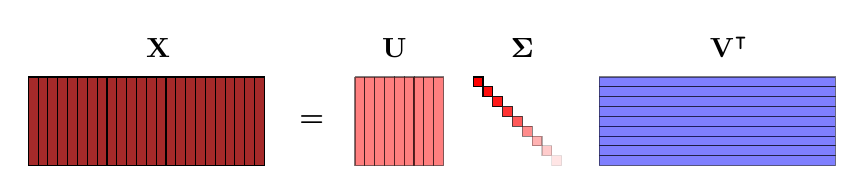
\begin{tikzpicture}[scale = 0.5]

  % draw line and angle
%  \draw 
%     pic [draw,angle radius=4mm,angle eccentricity=1.5, "$\theta$" font=\scriptsize] {angle=v2--v1--v3};
%\definecolor

\begin{scope}[xshift=7mm]
 

\draw [fill=Brown, opacity=1] (-16,4) -- (-15.75,4) -- (-15.75,1.75) -- (-16,1.75) -- (-16,4);
\draw [fill=Brown, opacity=1] (-15.75,4) -- (-15.5,4) -- (-15.5,1.75) -- (-15.75,1.75) -- (-15.75,4);

\draw [fill=Brown, opacity=1] (-15.5,4) -- (-15.25,4) -- (-15.25,1.75) -- (-15.5,1.75) -- (-15.5,4);
\draw [fill=Brown, opacity=1] (-15.25,4) -- (-15,4) -- (-15,1.75) -- (-15.25,1.75) -- (-15.25,4);
\draw [fill=Brown, opacity=1] (-15,4) -- (-14.75,4) -- (-14.75,1.75) -- (-15,1.75) -- (-15,4);
\draw [fill=Brown, opacity=1] (-14.75,4) -- (-14.5,4) -- (-14.5,1.75) -- (-14.75,1.75) -- (-14.75,4);
\draw [fill=Brown, opacity=1] (-14.5,4) -- (-14.25,4) -- (-14.25,1.75) -- (-14.5,1.75) -- (-14.5,4);
\draw [fill=Brown, opacity=1] (-14.25,4) -- (-14,4) -- (-14,1.75) -- (-14.25,1.75) -- (-14.25,4);
\draw [fill=Brown, opacity=1] (-14,4) -- (-13.75,4) -- (-13.75,1.75) -- (-14,1.75) -- (-14,4);
\draw [fill=Brown, opacity=1] (-13.75,4) -- (-13.5,4) -- (-13.5,1.75) -- (-13.75,1.75) -- (-13.75,4);
\draw [fill=Brown, opacity=1] (-13.5,4) -- (-13.25,4) -- (-13.25,1.75) -- (-13.5,1.75) -- (-13.5,4);
\draw [fill=Brown, opacity=1] (-13.25,4) -- (-13,4) -- (-13,1.75) -- (-13.25,1.75) -- (-13.25,4);
\draw [fill=Brown, opacity=1] (-13,4) -- (-12.75,4) -- (-12.75,1.75) -- (-13,1.75) -- (-13,4);

\draw [fill=Brown, opacity=1] (-12.75,4) -- (-12.5,4) -- (-12.5,1.75) -- (-12.75,1.75) -- (-12.75,4);
\draw [fill=Brown, opacity=1] (-12.5,4) -- (-12.25,4) -- (-12.25,1.75) -- (-12.5,1.75) -- (-12.5,4);
\draw [fill=Brown, opacity=1] (-12.25,4) -- (-12,4) -- (-12,1.75) -- (-12.25,1.75) -- (-12.25,4);
\draw [fill=Brown, opacity=1] (-12,4) -- (-11.75,4) -- (-11.75,1.75) -- (-12,1.75) -- (-12,4);

\draw [fill=Brown, opacity=1] (-11.75,4) -- (-11.5,4) -- (-11.5,1.75) -- (-11.75,1.75) -- (-11.75,4);
\draw [fill=Brown, opacity=1] (-11.5,4) -- (-11.25,4) -- (-11.25,1.75) -- (-11.5,1.75) -- (-11.5,4);
\draw [fill=Brown, opacity=1] (-11.25,4) -- (-11,4) -- (-11,1.75) -- (-11.25,1.75) -- (-11.25,4);
\draw [fill=Brown, opacity=1] (-11,4) -- (-10.75,4) -- (-10.75,1.75) -- (-11,1.75) -- (-11,4);
\draw [fill=Brown, opacity=1] (-10.75,4) -- (-10.5,4) -- (-10.5,1.75) -- (-10.75,1.75) -- (-10.75,4);
\draw [fill=Brown, opacity=1] (-10.5,4) -- (-10.25,4) -- (-10.25,1.75) -- (-10.5,1.75) -- (-10.5,4);
\draw [fill=Brown, opacity=1] (-10.25,4) -- (-10,4) -- (-10,1.75) -- (-10.25,1.75) -- (-10.25,4);


\end{scope}



\begin{scope}[xshift=0mm]
 
\draw [fill=red, opacity=0.5] (-7,4) -- (-6.75,4) -- (-6.75,1.75) -- (-7,1.75) -- (-7,4);
\draw [fill=red, opacity=0.5] (-6.75,4) -- (-6.5,4) -- (-6.5,1.75) -- (-6.75,1.75) -- (-6.75,4);
\draw [fill=red, opacity=0.5] (-6.5,4) -- (-6.25,4) -- (-6.25,1.75) -- (-6.5,1.75) -- (-6.5,4);

\draw [fill=red, opacity=0.5] (-6.25,4) -- (-6,4) -- (-6,1.75) -- (-6.25,1.75) -- (-6.25,4);
\draw [fill=red, opacity=0.5] (-6,4) -- (-5.75,4) -- (-5.75,1.75) -- (-6,1.75) -- (-6,4);
\draw [fill=red, opacity=0.5] (-5.75,4) -- (-5.5,4) -- (-5.5,1.75) -- (-5.75,1.75) -- (-5.75,4);
\draw [fill=red, opacity=0.5] (-5.5,4) -- (-5.25,4) -- (-5.25,1.75) -- (-5.5,1.75) -- (-5.5,4);

\draw [fill=red, opacity=0.5] (-5.25,4) -- (-5,4) -- (-5,1.75) -- (-5.25,1.75) -- (-5.25,4);
\draw [fill=red, opacity=0.5] (-5,4) -- (-4.75,4) -- (-4.75,1.75) -- (-5,1.75) -- (-5,4);
% \draw [fill=red, opacity=0.5] (-4.75,4) -- (-4.5,4) -- (-4.5,1.75) -- (-4.75,1.75) -- (-4.75,4);
% \draw [fill=red, opacity=0.5] (-4.5,4) -- (-4.25,4) -- (-4.25,1.75) -- (-4.5,1.75) -- (-4.5,4);


\end{scope}



\begin{scope}[xshift=-5mm]
 

\draw [fill=red, opacity=1] (-3.5,4) -- (-3.25,4) -- (-3.25,3.75) -- (-3.5,3.75) -- (-3.5,4);
\draw [fill=red, opacity=0.95] (-3.25,3.75) -- (-3,3.75) -- (-3,3.5) -- (-3.25,3.5) -- (-3.25,3.75);
\draw [fill=red, opacity=0.9] (-3,3.5) -- (-2.75,3.5) -- (-2.75,3.25) -- (-3,3.25) -- (-3,3.5);
\draw [fill=red, opacity=0.8] (-2.75,3.25) -- (-2.5,3.25) -- (-2.5,3) -- (-2.75,3) -- (-2.75,3.25);


\draw [fill=red, opacity=0.65] (-2.5,3) -- (-2.25,3) -- (-2.25,2.75) -- (-2.5,2.75) -- (-2.5,3);
\draw [fill=red, opacity=0.45] (-2.25,2.75) -- (-2,2.75) -- (-2,2.5) -- (-2.25,2.5) -- (-2.25,2.75);
\draw [fill=red, opacity=0.3] (-2,2.5) -- (-1.75,2.5) -- (-1.75,2.25) -- (-2,2.25) -- (-2,2.5);
\draw [fill=red, opacity=0.2] (-1.75,2.25) -- (-1.5,2.25) -- (-1.5,2) -- (-1.75,2) -- (-1.75,2.25);

\draw [fill=red, opacity=0.1] (-1.5,2) -- (-1.25,2) -- (-1.25,1.75) -- (-1.5,1.75) -- (-1.5,2);
\end{scope}


\begin{scope}[xshift=-18mm]
 
 
\draw [fill=blue, opacity=0.5] (7,3.75) -- (1,3.75) -- (1,4) -- (7,4) -- (7,3.75);
\draw [fill=blue, opacity=0.5] (7,3.5) -- (1,3.5) -- (1,3.75) -- (7,3.75) -- (7,3.5);
\draw [fill=blue, opacity=0.5] (7,3.25) -- (1,3.25) -- (1,3.5) -- (7,3.5) -- (7,3.25);
\draw [fill=blue, opacity=0.5] (7,3) -- (1,3) -- (1,3.25) -- (7,3.25) -- (7,3);
\draw [fill=blue, opacity=0.5] (7,2.75) -- (1,2.75) -- (1,3) -- (7,3) -- (7,2.75); 
\draw [fill=blue, opacity=0.5] (7,2.5) -- (1,2.5) -- (1,2.75) -- (7,2.75) -- (7,2.5);
\draw [fill=blue, opacity=0.5] (7,2.25) -- (1,2.25) -- (1,2.5) -- (7,2.5) -- (7,2.25);
\draw [fill=blue, opacity=0.5] (7,2) -- (1,2) -- (1,2.25) -- (7,2.25) -- (7,2);
\draw [fill=blue, opacity=0.5] (7,1.75) -- (1,1.75) -- (1,2) -- (7,2) -- (7,1.75);



\end{scope}




% \draw [fill=blue, opacity=0.5] (-16,3.75) -- (-10,3.75) -- (-10,4) -- (-16,4) -- (-16,3.75);
% \draw [fill=blue, opacity=0.5] (-16,3.5) -- (-10,3.5) -- (-10,3.75) -- (-16,3.75) -- (-16,3.5);
% \draw [fill=blue, opacity=0.5] (-16,3.25) -- (-10,3.25) -- (-10,3.5) -- (-16,3.5) -- (-16,3.25);
% \draw [fill=blue, opacity=0.5] (-16,3) -- (-10,3) -- (-10,3.25) -- (-16,3.25) -- (-16,3);
% \draw [fill=blue, opacity=0.5] (-16,2.75) -- (-10,2.75) -- (-10,3) -- (-16,3) -- (-16,2.75); 
% \draw [fill=blue, opacity=0.5] (-16,2.5) -- (-10,2.5) -- (-10,2.75) -- (-16,2.75) -- (-16,2.5);
% \draw [fill=blue, opacity=0.5] (-16,2.25) -- (-10,2.25) -- (-10,2.5) -- (-16,2.5) -- (-16,2.25);
% \draw [fill=blue, opacity=0.5] (-16,2) -- (-10,2) -- (-10,2.25) -- (-16,2.25) -- (-16,2);
% \draw [fill=blue, opacity=0.5] (-16,1.75) -- (-10,1.75) -- (-10,2) -- (-16,2) -- (-16,1.75);

\draw  (-12,4.25)  node [above] {$\bm{\mathrm{X}}$} ;
\draw  (-8.1,2.5)  node [above] {$\bm{=}$} ;

\draw  (-6,4.25)  node [above] {$\bm{\mathrm{U}}$} ;

\draw  (-2.75,4.25)  node [above] {$\bm{\mathrm{\Sigma}}$} ;

\draw  (2.5,4.25)  node [above] {$\bm{\mathrm{V}}^{\Tran}$} ;

%\draw  (-17.5,2.5)  node [above] {$\bm{V}^{\Tran}=$} ;


%\draw  (23,2)  node [above] {Complexity } ;

\end{tikzpicture}
}\\
     \subfloat[Sampling $k$ columns according to VS and our DPP]{

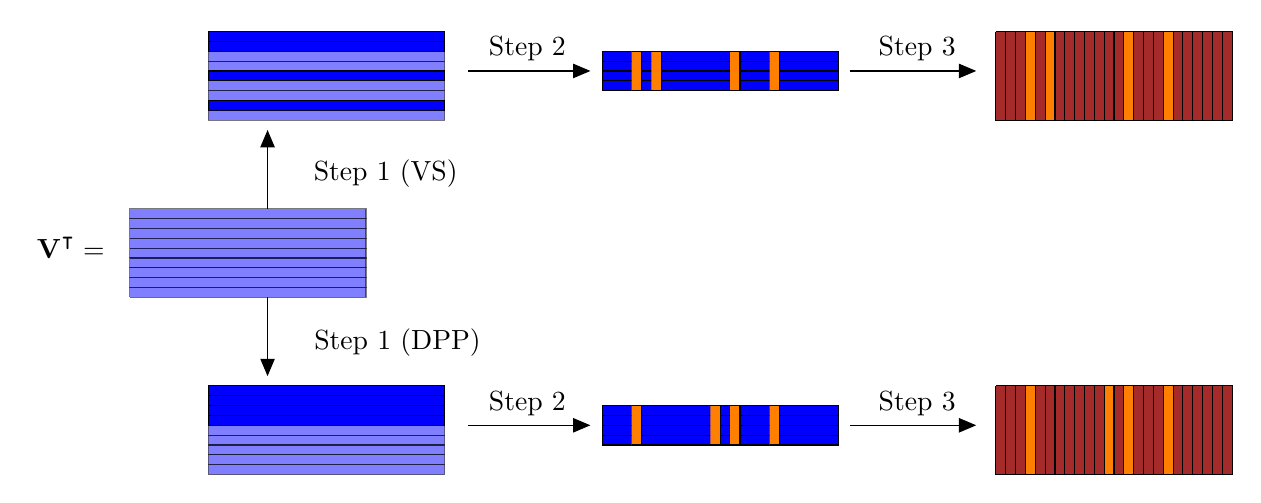
\begin{tikzpicture}[scale = 0.5]

  % draw line and angle
%  \draw
%     pic [draw,angle radius=4mm,angle eccentricity=1.5, "$\theta$" font=\scriptsize] {angle=v2--v1--v3};
\begin{scope}[yshift=-45mm]
\begin{scope}[xshift=-20mm]

\draw [fill=blue, opacity=0.5] (-16,3.75) -- (-10,3.75) -- (-10,4) -- (-16,4) -- (-16,3.75);
\draw [fill=blue, opacity=0.5] (-16,3.5) -- (-10,3.5) -- (-10,3.75) -- (-16,3.75) -- (-16,3.5);
\draw [fill=blue, opacity=0.5] (-16,3.25) -- (-10,3.25) -- (-10,3.5) -- (-16,3.5) -- (-16,3.25);
\draw [fill=blue, opacity=0.5] (-16,3) -- (-10,3) -- (-10,3.25) -- (-16,3.25) -- (-16,3);
\draw [fill=blue, opacity=0.5] (-16,2.75) -- (-10,2.75) -- (-10,3) -- (-16,3) -- (-16,2.75);
\draw [fill=blue, opacity=0.5] (-16,2.5) -- (-10,2.5) -- (-10,2.75) -- (-16,2.75) -- (-16,2.5);
\draw [fill=blue, opacity=0.5] (-16,2.25) -- (-10,2.25) -- (-10,2.5) -- (-16,2.5) -- (-16,2.25);
\draw [fill=blue, opacity=0.5] (-16,2) -- (-10,2) -- (-10,2.25) -- (-16,2.25) -- (-16,2);
\draw [fill=blue, opacity=0.5] (-16,1.75) -- (-10,1.75) -- (-10,2) -- (-16,2) -- (-16,1.75);


\draw  (-17.5,2.5)  node [above ] {$\bm{\mathrm{V}}^{\Tran} = $} ;

\draw  (-9.5,4.3)  node [above ] {Step 1 (VS)} ;

\draw [->] (-12.5,4) --  (-12.5,6);


\draw  (-9.2,0)  node [above ] {Step 1 (DPP)} ;

\draw [->] (-12.5,1.75) --  (-12.5,-0.25);

\end{scope}
\end{scope}





\begin{scope}[xshift=-120mm]


\draw [fill=blue, opacity=1] (-4,3.75) -- (2,3.75) -- (2,4) -- (-4,4) -- (-4,3.75);
\draw [fill=blue, opacity=1] (-4,3.5) -- (2,3.5) -- (2,3.75) -- (-4,3.75) -- (-4,3.5);
\draw [fill=blue, opacity=0.5] (-4,3.25) -- (2,3.25) -- (2,3.5) -- (-4,3.5) -- (-4,3.25);
\draw [fill=blue, opacity=0.5] (-4,3) -- (2,3) -- (2,3.25) -- (-4,3.25) -- (-4,3);
\draw [fill=blue, opacity=1] (-4,2.75) -- (2,2.75) -- (2,3) -- (-4,3) -- (-4,2.75);
\draw [fill=blue, opacity=0.5] (-4,2.5) -- (2,2.5) -- (2,2.75) -- (-4,2.75) -- (-4,2.5);
\draw [fill=blue, opacity=0.5] (-4,2.25) -- (2,2.25) -- (2,2.5) -- (-4,2.5) -- (-4,2.25);
\draw [fill=blue, opacity=1] (-4,2) -- (2,2) -- (2,2.25) -- (-4,2.25) -- (-4,2);
\draw [fill=blue, opacity=0.5] (-4,1.75) -- (2,1.75) -- (2,2) -- (-4,2) -- (-4,1.75);



\draw [->] (2.6,3) --  (4.1,3)  node [above] { Step 2 } --  (5.7,3);


\end{scope}


\begin{scope}[xshift=-120mm]
\begin{scope}[yshift=-90mm]


\draw [fill=blue, opacity=1] (-4,3.75) -- (2,3.75) -- (2,4) -- (-4,4) -- (-4,3.75);
\draw [fill=blue, opacity=1] (-4,3.5) -- (2,3.5) -- (2,3.75) -- (-4,3.75) -- (-4,3.5);
\draw [fill=blue, opacity=1] (-4,3.25) -- (2,3.25) -- (2,3.5) -- (-4,3.5) -- (-4,3.25);
\draw [fill=blue, opacity=1] (-4,3) -- (2,3) -- (2,3.25) -- (-4,3.25) -- (-4,3);
\draw [fill=blue, opacity=0.5] (-4,2.75) -- (2,2.75) -- (2,3) -- (-4,3) -- (-4,2.75);
\draw [fill=blue, opacity=0.5] (-4,2.5) -- (2,2.5) -- (2,2.75) -- (-4,2.75) -- (-4,2.5);
\draw [fill=blue, opacity=0.5] (-4,2.25) -- (2,2.25) -- (2,2.5) -- (-4,2.5) -- (-4,2.25);
\draw [fill=blue, opacity=0.5] (-4,2) -- (2,2) -- (2,2.25) -- (-4,2.25) -- (-4,2);
\draw [fill=blue, opacity=0.5] (-4,1.75) -- (2,1.75) -- (2,2) -- (-4,2) -- (-4,1.75);



\draw [->] (2.6,3) --  (4.1,3)  node [above] { Step 2 } --  (5.7,3);


\end{scope}
\end{scope}


\begin{scope}[xshift=-145mm]

\draw [fill=blue, opacity=1] (8.5,3.25) -- (14.5,3.25) -- (14.5,3.5) -- (8.5,3.5) -- (8.5,3.25);
\draw [fill=blue, opacity=1] (8.5,3) -- (14.5,3) -- (14.5,3.25) -- (8.5,3.25) -- (8.5,3);
\draw [fill=blue, opacity=1] (8.5,2.75) -- (14.5,2.75) -- (14.5,3) -- (8.5,3) -- (8.5,2.75);
\draw [fill=blue, opacity=1] (8.5,2.5) -- (14.5,2.5) -- (14.5,2.75) -- (8.5,2.75) -- (8.5,2.5);


\draw [fill=orange, opacity=1] (9.25,2.5) -- (9.25,2.5) -- (9.5,2.5) -- (9.5,3.5) -- (9.25,3.5);
\draw [fill=orange, opacity=1] (9.75,2.5) -- (9.75,2.5) -- (10,2.5) -- (10,3.5) -- (9.75,3.5);
\draw [fill=orange, opacity=1] (11.75,2.5) -- (11.75,2.5) -- (12,2.5) -- (12,3.5) -- (11.75,3.5);
\draw [fill=orange, opacity=1] (12.75,2.5) -- (12.75,2.5) -- (13,2.5) -- (13,3.5) -- (12.75,3.5);



\draw [->] (14.8,3) --  (16.5,3)  node [above] { Step 3 } --  (18,3);

\end{scope}

\begin{scope}[yshift=-90mm]
\begin{scope}[xshift=-145mm]

\draw [fill=blue, opacity=1] (8.5,3.25) -- (14.5,3.25) -- (14.5,3.5) -- (8.5,3.5) -- (8.5,3.25);
\draw [fill=blue, opacity=1] (8.5,3) -- (14.5,3) -- (14.5,3.25) -- (8.5,3.25) -- (8.5,3);
\draw [fill=blue, opacity=1] (8.5,2.75) -- (14.5,2.75) -- (14.5,3) -- (8.5,3) -- (8.5,2.75);
\draw [fill=blue, opacity=1] (8.5,2.5) -- (14.5,2.5) -- (14.5,2.75) -- (8.5,2.75) -- (8.5,2.5);


\draw [fill=orange, opacity=1] (9.25,2.5) -- (9.25,2.5) -- (9.5,2.5) -- (9.5,3.5) -- (9.25,3.5);
\draw [fill=orange, opacity=1] (11.25,2.5) -- (11.25,2.5) -- (11.5,2.5) -- (11.5,3.5) -- (11.25,3.5);
\draw [fill=orange, opacity=1] (11.75,2.5) -- (11.75,2.5) -- (12,2.5) -- (12,3.5) -- (11.75,3.5);
\draw [fill=orange, opacity=1] (12.75,2.5) -- (12.75,2.5) -- (13,2.5) -- (13,3.5) -- (12.75,3.5);



\draw [->] (14.8,3) --  (16.5,3)  node [above] { Step 3 } --  (18,3);

\end{scope}
\end{scope}

%\begin{scope}[yshift=-45mm]
\begin{scope}[xshift=200mm]
 

\draw [fill=Brown, opacity=1] (-16,4) -- (-15.75,4) -- (-15.75,1.75) -- (-16,1.75) -- (-16,4);
\draw [fill=Brown, opacity=1] (-15.75,4) -- (-15.5,4) -- (-15.5,1.75) -- (-15.75,1.75) -- (-15.75,4);

\draw [fill=Brown, opacity=1] (-15.5,4) -- (-15.25,4) -- (-15.25,1.75) -- (-15.5,1.75) -- (-15.5,4);
\draw [fill=orange, opacity=1] (-15.25,4) -- (-15,4) -- (-15,1.75) -- (-15.25,1.75) -- (-15.25,4);
\draw [fill=Brown, opacity=1] (-15,4) -- (-14.75,4) -- (-14.75,1.75) -- (-15,1.75) -- (-15,4);
\draw [fill=orange, opacity=1] (-14.75,4) -- (-14.5,4) -- (-14.5,1.75) -- (-14.75,1.75) -- (-14.75,4);
\draw [fill=Brown, opacity=1] (-14.5,4) -- (-14.25,4) -- (-14.25,1.75) -- (-14.5,1.75) -- (-14.5,4);
\draw [fill=Brown, opacity=1] (-14.25,4) -- (-14,4) -- (-14,1.75) -- (-14.25,1.75) -- (-14.25,4);
\draw [fill=Brown, opacity=1] (-14,4) -- (-13.75,4) -- (-13.75,1.75) -- (-14,1.75) -- (-14,4);
\draw [fill=Brown, opacity=1] (-13.75,4) -- (-13.5,4) -- (-13.5,1.75) -- (-13.75,1.75) -- (-13.75,4);
\draw [fill=Brown, opacity=1] (-13.5,4) -- (-13.25,4) -- (-13.25,1.75) -- (-13.5,1.75) -- (-13.5,4);
\draw [fill=Brown, opacity=1] (-13.25,4) -- (-13,4) -- (-13,1.75) -- (-13.25,1.75) -- (-13.25,4);
\draw [fill=Brown, opacity=1] (-13,4) -- (-12.75,4) -- (-12.75,1.75) -- (-13,1.75) -- (-13,4);

\draw [fill=orange, opacity=1] (-12.75,4) -- (-12.5,4) -- (-12.5,1.75) -- (-12.75,1.75) -- (-12.75,4);
\draw [fill=Brown, opacity=1] (-12.5,4) -- (-12.25,4) -- (-12.25,1.75) -- (-12.5,1.75) -- (-12.5,4);
\draw [fill=Brown, opacity=1] (-12.25,4) -- (-12,4) -- (-12,1.75) -- (-12.25,1.75) -- (-12.25,4);
\draw [fill=Brown, opacity=1] (-12,4) -- (-11.75,4) -- (-11.75,1.75) -- (-12,1.75) -- (-12,4);

\draw [fill=orange, opacity=1] (-11.75,4) -- (-11.5,4) -- (-11.5,1.75) -- (-11.75,1.75) -- (-11.75,4);
\draw [fill=Brown, opacity=1] (-11.5,4) -- (-11.25,4) -- (-11.25,1.75) -- (-11.5,1.75) -- (-11.5,4);
\draw [fill=Brown, opacity=1] (-11.25,4) -- (-11,4) -- (-11,1.75) -- (-11.25,1.75) -- (-11.25,4);
\draw [fill=Brown, opacity=1] (-11,4) -- (-10.75,4) -- (-10.75,1.75) -- (-11,1.75) -- (-11,4);
\draw [fill=Brown, opacity=1] (-10.75,4) -- (-10.5,4) -- (-10.5,1.75) -- (-10.75,1.75) -- (-10.75,4);
\draw [fill=Brown, opacity=1] (-10.5,4) -- (-10.25,4) -- (-10.25,1.75) -- (-10.5,1.75) -- (-10.5,4);
\draw [fill=Brown, opacity=1] (-10.25,4) -- (-10,4) -- (-10,1.75) -- (-10.25,1.75) -- (-10.25,4);


\end{scope}
%\end{scope}


\begin{scope}[yshift=-90mm]
\begin{scope}[xshift=200mm]
 

\draw [fill=Brown, opacity=1] (-16,4) -- (-15.75,4) -- (-15.75,1.75) -- (-16,1.75) -- (-16,4);
\draw [fill=Brown, opacity=1] (-15.75,4) -- (-15.5,4) -- (-15.5,1.75) -- (-15.75,1.75) -- (-15.75,4);

\draw [fill=Brown, opacity=1] (-15.5,4) -- (-15.25,4) -- (-15.25,1.75) -- (-15.5,1.75) -- (-15.5,4);
\draw [fill=orange, opacity=1] (-15.25,4) -- (-15,4) -- (-15,1.75) -- (-15.25,1.75) -- (-15.25,4);
\draw [fill=Brown, opacity=1] (-15,4) -- (-14.75,4) -- (-14.75,1.75) -- (-15,1.75) -- (-15,4);
\draw [fill=Brown, opacity=1] (-14.75,4) -- (-14.5,4) -- (-14.5,1.75) -- (-14.75,1.75) -- (-14.75,4);
\draw [fill=Brown, opacity=1] (-14.5,4) -- (-14.25,4) -- (-14.25,1.75) -- (-14.5,1.75) -- (-14.5,4);
\draw [fill=Brown, opacity=1] (-14.25,4) -- (-14,4) -- (-14,1.75) -- (-14.25,1.75) -- (-14.25,4);
\draw [fill=Brown, opacity=1] (-14,4) -- (-13.75,4) -- (-13.75,1.75) -- (-14,1.75) -- (-14,4);
\draw [fill=Brown, opacity=1] (-13.75,4) -- (-13.5,4) -- (-13.5,1.75) -- (-13.75,1.75) -- (-13.75,4);
\draw [fill=Brown, opacity=1] (-13.5,4) -- (-13.25,4) -- (-13.25,1.75) -- (-13.5,1.75) -- (-13.5,4);
\draw [fill=orange, opacity=1] (-13.25,4) -- (-13,4) -- (-13,1.75) -- (-13.25,1.75) -- (-13.25,4);
\draw [fill=Brown, opacity=1] (-13,4) -- (-12.75,4) -- (-12.75,1.75) -- (-13,1.75) -- (-13,4);

\draw [fill=orange, opacity=1] (-12.75,4) -- (-12.5,4) -- (-12.5,1.75) -- (-12.75,1.75) -- (-12.75,4);
\draw [fill=Brown, opacity=1] (-12.5,4) -- (-12.25,4) -- (-12.25,1.75) -- (-12.5,1.75) -- (-12.5,4);
\draw [fill=Brown, opacity=1] (-12.25,4) -- (-12,4) -- (-12,1.75) -- (-12.25,1.75) -- (-12.25,4);
\draw [fill=Brown, opacity=1] (-12,4) -- (-11.75,4) -- (-11.75,1.75) -- (-12,1.75) -- (-12,4);

\draw [fill=orange, opacity=1] (-11.75,4) -- (-11.5,4) -- (-11.5,1.75) -- (-11.75,1.75) -- (-11.75,4);
\draw [fill=Brown, opacity=1] (-11.5,4) -- (-11.25,4) -- (-11.25,1.75) -- (-11.5,1.75) -- (-11.5,4);
\draw [fill=Brown, opacity=1] (-11.25,4) -- (-11,4) -- (-11,1.75) -- (-11.25,1.75) -- (-11.25,4);
\draw [fill=Brown, opacity=1] (-11,4) -- (-10.75,4) -- (-10.75,1.75) -- (-11,1.75) -- (-11,4);
\draw [fill=Brown, opacity=1] (-10.75,4) -- (-10.5,4) -- (-10.5,1.75) -- (-10.75,1.75) -- (-10.75,4);
\draw [fill=Brown, opacity=1] (-10.5,4) -- (-10.25,4) -- (-10.25,1.75) -- (-10.5,1.75) -- (-10.5,4);
\draw [fill=Brown, opacity=1] (-10.25,4) -- (-10,4) -- (-10,1.75) -- (-10.25,1.75) -- (-10.25,4);


\end{scope}
\end{scope}

% \begin{scope}[xshift=-50mm]





% \end{scope}

%\draw  (23,2)  node [above] {Complexity } ;

\end{tikzpicture}
}
  %  \subfloat[]{

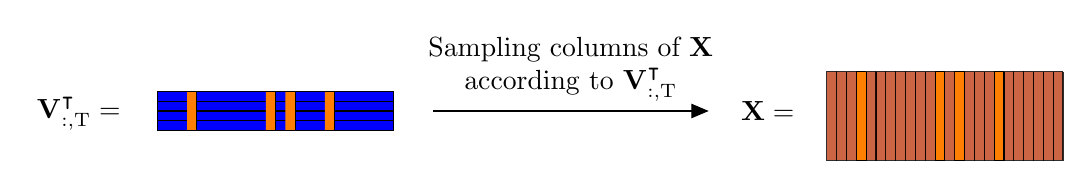
\begin{tikzpicture}[scale = 0.5]

  % draw line and angle
%  \draw 
%     pic [draw,angle radius=4mm,angle eccentricity=1.5, "$\theta$" font=\scriptsize] {angle=v2--v1--v3};

\begin{scope}[xshift=-65mm]



\draw [fill=blue, opacity=1] (0.5,3.25) -- (6.5,3.25) -- (6.5,3.5) -- (0.5,3.5) -- (0.5,3.25);
\draw [fill=blue, opacity=1] (0.5,3) -- (6.5,3) -- (6.5,3.25) -- (0.5,3.25) -- (0.5,3);
\draw [fill=blue, opacity=1] (0.5,2.75) -- (6.5,2.75) -- (6.5,3) -- (0.5,3) -- (0.5,2.75);
\draw [fill=blue, opacity=1] (0.5,2.5) -- (6.5,2.5) -- (6.5,2.75) -- (0.5,2.75) -- (0.5,2.5);


\draw [fill=orange, opacity=1] (1.25,2.5) -- (1.25,2.5) -- (1.5,2.5) -- (1.5,3.5) -- (1.25,3.5);
\draw [fill=orange, opacity=1] (3.25,2.5) -- (3.25,2.5) -- (3.5,2.5) -- (3.5,3.5) -- (3.25,3.5);
\draw [fill=orange, opacity=1] (3.75,2.5) -- (3.75,2.5) -- (4,2.5) -- (4,3.5) -- (3.75,3.5);
\draw [fill=orange, opacity=1] (4.75,2.5) -- (4.75,2.5) -- (5,2.5) -- (5,3.5) -- (4.75,3.5);


 \draw  (-1.5,2.25)  node [above] {$\bm{\mathrm{V}}_{:,\mathrm{T}}^{\Tran}=$} ;
\end{scope}

\begin{scope}[xshift=10mm]


\draw [fill=Bittersweet, opacity=0.8] (16,4) -- (15.75,4) -- (15.75,1.75) -- (16,1.75) -- (16,4);
\draw [fill=Bittersweet, opacity=0.8] (15.75,4) -- (15.5,4) -- (15.5,1.75) -- (15.75,1.75) -- (15.75,4);

\draw [fill=Bittersweet, opacity=0.8] (15.5,4) -- (15.25,4) -- (15.25,1.75) -- (15.5,1.75) -- (15.5,4);
\draw [fill=Bittersweet, opacity=0.8] (15.25,4) -- (15,4) -- (15,1.75) -- (15.25,1.75) -- (15.25,4);
\draw [fill=Bittersweet, opacity=0.8] (15,4) -- (14.75,4) -- (14.75,1.75) -- (15,1.75) -- (15,4);
\draw [fill=Bittersweet, opacity=0.8] (14.75,4) -- (14.5,4) -- (14.5,1.75) -- (14.75,1.75) -- (14.75,4);
\draw [fill=orange, opacity=1] (14.5,4) -- (14.25,4) -- (14.25,1.75) -- (14.5,1.75) -- (14.5,4);
\draw [fill=Bittersweet, opacity=0.8] (14.25,4) -- (14,4) -- (14,1.75) -- (14.25,1.75) -- (14.25,4);
\draw [fill=Bittersweet, opacity=0.8] (14,4) -- (13.75,4) -- (13.75,1.75) -- (14,1.75) -- (14,4);
\draw [fill=Bittersweet, opacity=0.8] (13.75,4) -- (13.5,4) -- (13.5,1.75) -- (13.75,1.75) -- (13.75,4);
\draw [fill=orange, opacity=1] (13.5,4) -- (13.25,4) -- (13.25,1.75) -- (13.5,1.75) -- (13.5,4);
\draw [fill=Bittersweet, opacity=0.8] (13.25,4) -- (13,4) -- (13,1.75) -- (13.25,1.75) -- (13.25,4);
\draw [fill=orange, opacity=1] (13,4) -- (12.75,4) -- (12.75,1.75) -- (13,1.75) -- (13,4);

\draw [fill=Bittersweet, opacity=0.8] (12.75,4) -- (12.5,4) -- (12.5,1.75) -- (12.75,1.75) -- (12.75,4);
\draw [fill=Bittersweet, opacity=0.8] (12.5,4) -- (12.25,4) -- (12.25,1.75) -- (12.5,1.75) -- (12.5,4);
\draw [fill=Bittersweet, opacity=0.8] (12.25,4) -- (12,4) -- (12,1.75) -- (12.25,1.75) -- (12.25,4);
\draw [fill=Bittersweet, opacity=0.8] (12,4) -- (11.75,4) -- (11.75,1.75) -- (12,1.75) -- (12,4);

\draw [fill=Bittersweet, opacity=0.8] (11.75,4) -- (11.5,4) -- (11.5,1.75) -- (11.75,1.75) -- (11.75,4);
\draw [fill=Bittersweet, opacity=0.8] (11.5,4) -- (11.25,4) -- (11.25,1.75) -- (11.5,1.75) -- (11.5,4);
\draw [fill=Bittersweet, opacity=0.8] (11.25,4) -- (11,4) -- (11,1.75) -- (11.25,1.75) -- (11.25,4);
\draw [fill=orange, opacity=1] (11,4) -- (10.75,4) -- (10.75,1.75) -- (11,1.75) -- (11,4);
\draw [fill=Bittersweet, opacity=0.8] (10.75,4) -- (10.5,4) -- (10.5,1.75) -- (10.75,1.75) -- (10.75,4);
\draw [fill=Bittersweet, opacity=0.8] (10.5,4) -- (10.25,4) -- (10.25,1.75) -- (10.5,1.75) -- (10.5,4);
\draw [fill=Bittersweet, opacity=0.8] (10.25,4) -- (10,4) -- (10,1.75) -- (10.25,1.75) -- (10.25,4);


\draw  (8.5,2.5)  node [above] {$\bm{\mathrm{X}} = $} ;
\end{scope}


\draw [->] (1,3) --  (4.5,3)  node [above] {} --  (8,3);

\draw  (4.5,3)  node [above , align=center] {Sampling columns of $\bm{\mathrm{X}}$\\ according to $\bm{\mathrm{V}}_{:,\mathrm{T}}^{\Tran}$} ;



% \draw [->] (-9.5,3) --  (-7.5,3)  node [above] { $\Prb(T)$} --  (-5,3);

% \draw [->] (3,3) --  (5,3)  node [above] { $\Prb(S|T)$} --  (7.5,3);


% \draw  (-7.5,4.25)  node [above] {Step 1} ;

% \draw  (5,4.25)  node [above] {Step 2} ;

%\draw  (23,2)  node [above] {Complexity } ;

\end{tikzpicture}
}\\
    %\caption{DPP sampling algorithm
    %\label{f:dpp_sampling_algorithm}
    %}
%    \subfloat[]{

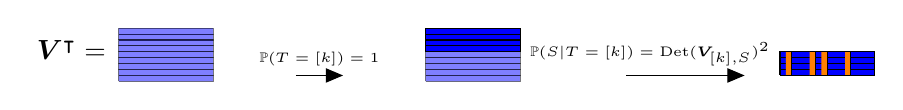
\begin{tikzpicture}[scale = 0.3]

  % draw line and angle
%  \draw 
%     pic [draw,angle radius=4mm,angle eccentricity=1.5, "$\theta$" font=\scriptsize] {angle=v2--v1--v3};

 



 

\draw [fill=blue, opacity=0.5] (-15,3.75) -- (-11,3.75) -- (-11,4) -- (-15,4) -- (-15,3.75);
\draw [fill=blue, opacity=0.5] (-15,3.5) -- (-11,3.5) -- (-11,3.75) -- (-15,3.75) -- (-15,3.5);
\draw [fill=blue, opacity=0.5] (-15,3.25) -- (-11,3.25) -- (-11,3.5) -- (-15,3.5) -- (-15,3.25);
\draw [fill=blue, opacity=0.5] (-15,3) -- (-11,3) -- (-11,3.25) -- (-15,3.25) -- (-15,3);
\draw [fill=blue, opacity=0.5] (-15,2.75) -- (-11,2.75) -- (-11,3) -- (-15,3) -- (-15,2.75); 
\draw [fill=blue, opacity=0.5] (-15,2.5) -- (-11,2.5) -- (-11,2.75) -- (-15,2.75) -- (-15,2.5);
\draw [fill=blue, opacity=0.5] (-15,2.25) -- (-11,2.25) -- (-11,2.5) -- (-15,2.5) -- (-15,2.25);
\draw [fill=blue, opacity=0.5] (-15,2) -- (-11,2) -- (-11,2.25) -- (-15,2.25) -- (-15,2);
\draw [fill=blue, opacity=0.5] (-15,1.75) -- (-11,1.75) -- (-11,2) -- (-15,2) -- (-15,1.75);



\draw [fill=blue, opacity=1] (-2,3.75) -- (2,3.75) -- (2,4) -- (-2,4) -- (-2,3.75);
\draw [fill=blue, opacity=1] (-2,3.5) -- (2,3.5) -- (2,3.75) -- (-2,3.75) -- (-2,3.5);
\draw [fill=blue, opacity=1] (-2,3.25) -- (2,3.25) -- (2,3.5) -- (-2,3.5) -- (-2,3.25);
\draw [fill=blue, opacity=1] (-2,3) -- (2,3) -- (2,3.25) -- (-2,3.25) -- (-2,3);
\draw [fill=blue, opacity=0.5] (-2,2.75) -- (2,2.75) -- (2,3) -- (-2,3) -- (-2,2.75); 
\draw [fill=blue, opacity=0.5] (-2,2.5) -- (2,2.5) -- (2,2.75) -- (-2,2.75) -- (-2,2.5);
\draw [fill=blue, opacity=0.5] (-2,2.25) -- (2,2.25) -- (2,2.5) -- (-2,2.5) -- (-2,2.25);
\draw [fill=blue, opacity=0.5] (-2,2) -- (2,2) -- (2,2.25) -- (-2,2.25) -- (-2,2);
\draw [fill=blue, opacity=0.5] (-2,1.75) -- (2,1.75) -- (2,2) -- (-2,2) -- (-2,1.75);





\draw [fill=blue, opacity=1] (13,2.75) -- (17,2.75) -- (17,3) -- (13,3) -- (13,2.75);
\draw [fill=blue, opacity=1] (13,2.5) -- (17,2.5) -- (17,2.75) -- (13,2.75) -- (13,2.5);
\draw [fill=blue, opacity=1] (13,2.25) -- (17,2.25) -- (17,2.5) -- (13,2.5) -- (13,2.25);
\draw [fill=blue, opacity=1] (13,2) -- (17,2) -- (17,2.25) -- (13,2.25) -- (13,2);


\draw [fill=orange, opacity=1] (13.25,2) -- (13.25,2) -- (13.5,2) -- (13.5,3) -- (13.25,3);
\draw [fill=orange, opacity=1] (14.25,2) -- (14.25,2) -- (14.5,2) -- (14.5,3) -- (14.25,3);
\draw [fill=orange, opacity=1] (14.75,2) -- (14.75,2) -- (15,2) -- (15,3) -- (14.75,3);
\draw [fill=orange, opacity=1] (15.75,2) -- (15.75,2) -- (16,2) -- (16,3) -- (15.75,3);



\draw [->] (-7.5,2) --  (-6.5,2)  node [above] {\tiny $\Prb(T = [k]) = 1$} --  (-5.5,2);

\draw [->] (6.5,2) --  (7.5,2)  node [above] {\tiny $\Prb(S|T = [k]) = \Det (\bm{V}_{[k],S})^{2}$} --  (11.5,2);

\draw  (-17,2.25)  node [above] {$\bm{V}^{\Tran}=$} ;

\end{tikzpicture}
}\\
%\subfloat[]{

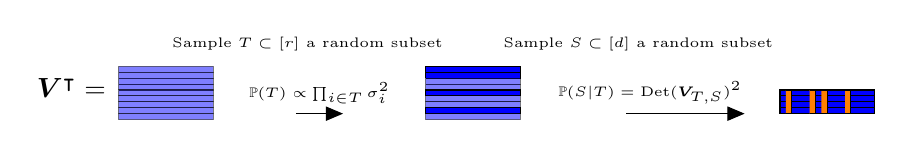
\begin{tikzpicture}[scale = 0.3]

  % draw line and angle
%  \draw 
%     pic [draw,angle radius=4mm,angle eccentricity=1.5, "$\theta$" font=\scriptsize] {angle=v2--v1--v3};

 

\draw [fill=blue, opacity=0.5] (-15,3.75) -- (-11,3.75) -- (-11,4) -- (-15,4) -- (-15,3.75);
\draw [fill=blue, opacity=0.5] (-15,3.5) -- (-11,3.5) -- (-11,3.75) -- (-15,3.75) -- (-15,3.5);
\draw [fill=blue, opacity=0.5] (-15,3.25) -- (-11,3.25) -- (-11,3.5) -- (-15,3.5) -- (-15,3.25);
\draw [fill=blue, opacity=0.5] (-15,3) -- (-11,3) -- (-11,3.25) -- (-15,3.25) -- (-15,3);
\draw [fill=blue, opacity=0.5] (-15,2.75) -- (-11,2.75) -- (-11,3) -- (-15,3) -- (-15,2.75); 
\draw [fill=blue, opacity=0.5] (-15,2.5) -- (-11,2.5) -- (-11,2.75) -- (-15,2.75) -- (-15,2.5);
\draw [fill=blue, opacity=0.5] (-15,2.25) -- (-11,2.25) -- (-11,2.5) -- (-15,2.5) -- (-15,2.25);
\draw [fill=blue, opacity=0.5] (-15,2) -- (-11,2) -- (-11,2.25) -- (-15,2.25) -- (-15,2);
\draw [fill=blue, opacity=0.5] (-15,1.75) -- (-11,1.75) -- (-11,2) -- (-15,2) -- (-15,1.75);



\draw [fill=blue, opacity=1] (-2,3.75) -- (2,3.75) -- (2,4) -- (-2,4) -- (-2,3.75);
\draw [fill=blue, opacity=1] (-2,3.5) -- (2,3.5) -- (2,3.75) -- (-2,3.75) -- (-2,3.5);
\draw [fill=blue, opacity=0.5] (-2,3.25) -- (2,3.25) -- (2,3.5) -- (-2,3.5) -- (-2,3.25);
\draw [fill=blue, opacity=0.5] (-2,3) -- (2,3) -- (2,3.25) -- (-2,3.25) -- (-2,3);
\draw [fill=blue, opacity=1] (-2,2.75) -- (2,2.75) -- (2,3) -- (-2,3) -- (-2,2.75); 
\draw [fill=blue, opacity=0.5] (-2,2.5) -- (2,2.5) -- (2,2.75) -- (-2,2.75) -- (-2,2.5);
\draw [fill=blue, opacity=0.5] (-2,2.25) -- (2,2.25) -- (2,2.5) -- (-2,2.5) -- (-2,2.25);
\draw [fill=blue, opacity=1] (-2,2) -- (2,2) -- (2,2.25) -- (-2,2.25) -- (-2,2);
\draw [fill=blue, opacity=0.5] (-2,1.75) -- (2,1.75) -- (2,2) -- (-2,2) -- (-2,1.75);





\draw [fill=blue, opacity=1] (13,2.75) -- (17,2.75) -- (17,3) -- (13,3) -- (13,2.75);
\draw [fill=blue, opacity=1] (13,2.5) -- (17,2.5) -- (17,2.75) -- (13,2.75) -- (13,2.5);
\draw [fill=blue, opacity=1] (13,2.25) -- (17,2.25) -- (17,2.5) -- (13,2.5) -- (13,2.25);
\draw [fill=blue, opacity=1] (13,2) -- (17,2) -- (17,2.25) -- (13,2.25) -- (13,2);


\draw [fill=orange, opacity=1] (13.25,2) -- (13.25,2) -- (13.5,2) -- (13.5,3) -- (13.25,3);
\draw [fill=orange, opacity=1] (14.25,2) -- (14.25,2) -- (14.5,2) -- (14.5,3) -- (14.25,3);
\draw [fill=orange, opacity=1] (14.75,2) -- (14.75,2) -- (15,2) -- (15,3) -- (14.75,3);
\draw [fill=orange, opacity=1] (15.75,2) -- (15.75,2) -- (16,2) -- (16,3) -- (15.75,3);



\draw [->] (-7.5,2) --  (-6.5,2)  node [above] {\tiny $\Prb(T) \propto \prod_{i \in T} \sigma_{i}^{2}$} --  (-5.5,2);

\draw [->] (6.5,2) --  (7.5,2)  node [above] {\tiny $\Prb(S|T) = \Det (\bm{V}_{T,S})^{2}$} --  (11.5,2);

\draw  (-17,2.25)  node [above] {$\bm{V}^{\Tran}=$} ;

\draw  (-7,4.25)  node [above] {\tiny Sample $T \subset [r]$ a random subset} ;

\draw  (7,4.25)  node [above] {\tiny Sample $S \subset [d]$ a random subset} ;

%\draw  (23,2)  node [above] {Complexity } ;

\end{tikzpicture}
}
    %\caption{Volume sampling algorithm
    %label{f:volume_sampling_algorithm}
    %}
    \caption{A graphical depiction of the sampling algorithms for volume sampling (VS) and the DPP with marginal kernel $\bm{V}^{}_{k}\bm{V}_{k}^{\Tran}$. (a) Both algorithms start with an SVD. (b) In Step 1, VS randomly selects $k$ rows of $\bm V^{\Tran}$, while our DPP always picks the first $k$ rows. Step 2 is the same for both algorithms: jointly sample $k$ columns of the subsampled $\bm V^{\Tran}$, proportionally to their squared volume. Finally, Step 3 is simply the extraction of the corresponding columns of $\bm X$.
    %The common steps on the sampling algorithm for DPPs and volume sampling. Step 1: sample a random subset of right eigenvectors $T \subseteq [r]$with probability $\Prb(T)$. Step 2: sample a random subset of columns indices $S \subseteq [d]$ with probability $\Prb(S|T)$.
    \label{f:sampling}
    }
\end{figure}

% \begin{table}
% \centering
%  \begin{tabular}{| c| c| c|}
%  \hline
%   - & Step 1 & Step 2\\
%  \hline
%  Projection DPP & $\Prb(T=[k]) = 1$ & $\Prb(S|T) = \Det (\bm{V}_{S,[k]})^{2}$\\
%  \hline
%  DPP & $\Prb(t \in T) = \lambda_{t}$ & $\Prb(S|T) = \Det (\bm{V}_{S,T})^{2}$\\
%  \hline
%  Volume sampling & $\Prb(T) \propto \prod_{i \in T} \sigma_{i}^{2}$ & $\Prb(S|T) = \Det (\bm{V}_{S,T})^{2}$\\
%  \hline
% \end{tabular}
% \caption{Differences in sampling schemes between projection DPP, DPP and volume sampling.}
% \end{table}

A fundamental example of $k$-DPPs is volume sampling, as defined in Section \ref{subsec:volume_sampling}. Its kernel is the Gram matrix of the data $\bm{L} = \bm{X}^{\Tran}\bm{X}$. In general, $\bm{L}$ is not an orthogonal projection matrix, so that volume sampling is not a DPP. \rev{In particular, draws from volume sampling have fixed cardinality, and thus cannot be written as a sum of non trivial Bernoulli random variables.}

\subsection{Motivations for column subset selection using projection DPPs}
Volume sampling has been successfully used for column subset selection, see Section~\ref{subsec:volume_sampling}. Our motivation to investigate projection DPPs instead of volume sampling is twofold.

Following \eqref{eq:volume_sampling_as_mixture_equation}, volume sampling can be seen as a mixture of projection DPPs indexed by $T\subseteq [d], \vert T\vert=k$, with marginal kernels $\bm{K}_{T} = \bm{V}^{}_{:,T}\bm{V}^{\Tran}_{:,T}$ and mixture weights $\mu_{T} \propto \prod_{i \in T} \sigma_{i}^{2}$. The component with the highest weight thus corresponds to the $k$ largest singular values, that is, the projection DPP with marginal kernel
$\bm K:=\bm{V}^{}_{k}\bm{V}_{k}^{\Tran}$. This paper is about column subset selection using precisely this DPP. Alternately, we could motivate the study of this DPP by remarking that its marginals $\Prb({i}\subseteq Y)$ are the $k$-leverage scores introduced in Section~\ref{subsec:k-lvs_sampling}. Since $\bm K$ is symmetric, this DPP can be seen as a repulsive generalization of leverage score sampling.

Finally, we recap the difference between volume sampling and the DPP with kernel $\bm K$ with a graphical depiction in Figure~\ref{f:sampling} of the two procedures to sample from them that we introduced in Section~\ref{subsec:sampling_from_a_dpp}. Figure~\ref{f:sampling} is another illustration of the decomposition of volume sampling as a mixture of projection DPPs.


\section{Main results}
%!TEX root=./submitted.tex
In this section, we prove bounds for $\EX_{\DPP} \| \bm{X} - \Pi_{S}^{\nu}\bm{X} \|^2_{\nu}$ under the projection DPP of marginal kernel $\bm{K} = \bm{V}^{}_{k}\bm{V}^{\Tran}_{k}$ presented in Section~\ref{s:dppsection}. Throughout, we compare our bounds to the state-of-the-art bounds of volume sampling obtained by \cite{DRVW06}; see Theorem~\ref{thrm:volume_sampling_theorem} and Section~\ref{subsec:volume_sampling}. For clarity, we defer the proofs of our results from this section to Appendix~\ref{app:proofs}.

%\subsection{State of the art}\label{volume_sampling_proof_section}
% \begin{proposition}[\citealp{DRVW06}] \label{volume_sampling_fro_proof}
% Let $S$ be a random subset of $k$ columns of $\bm{X}$ chosen according to volume sampling,
% \begin{equation}
% \Prb_{\VS}(S) \propto \Det(\bm{C}^{\Tran}\bm{C}), \quad \bm{C} = \bm{X}_{:,S}.
% \end{equation}
% %with $$.\\
% We have
% \begin{equation}\label{eq:spectral_volume_sampling}
%   \EX_{\VS} \| \bm{X} - \Pi_{S}\bm{X} \|_{2}^{2}
%   \leq (k+1)(d-k) \| \bm{X} - \Pi_{k}\bm{X} \|_{2}^{2}
% \end{equation}
% and
% \begin{equation}\label{eq:frobenius_volume_sampling}
%   \EX_{\VS} \| \bm{X} - \Pi_{S}\bm{X} \|_{\Fr}^{2}
%   = (k+1)\frac{e_{k+1}(\bm{\sigma}^{2})}{e_{k}(\bm{\sigma}^{2})} \leq (k+1) \| \bm{X} - \Pi_{k}\bm{X} \|_{\Fr}^{2}.
% \end{equation}
% \end{proposition}
%

%%%%%%%
\subsection{Multiplicative bounds in spectral and Frobenius norm}
\label{sec:new_results_randomized}
Let $S$ be a random subset of $k$ columns of $\bm{X}$ chosen with probability:
\begin{equation}
	\Prb_{\DPP}(S) = \Det(\bm{V}_{S,[k]})^{2}.
\end{equation}
First, without any further assumption, we have the following result.
%% Proposition
\begin{proposition}
    \label{projection_dpp_theorem}
    Under the projection DPP of marginal kernel $\bm{V}^{}_{k}\bm{V}^{\Tran}_{k}$, it holds that
    \begin{equation}
    	\label{eq:projection_dpp_theorem}
    	\EX_{\DPP} \| \bm{X} - \Pi_{S}^{\nu}\bm{X} \|_{\nu}^{2} \leq k(d+1-k)\| \bm{X} - \Pi_{k}\bm{X} \|_{\nu}^{2}, \quad \nu\in\{2,\Fr\}.
    \end{equation}
\end{proposition}
%%%
For the spectral norm, the bound is practically the same as that of volume sampling \eqref{e:vsBound2}. However, our bound for the Frobenius norm is worse than \eqref{e:vsBoundFr} by a factor $(d-k)$. In the rest of this section, we sharpen our bounds by taking into account the sparsity level of the $k$-leverage scores and the decay of singular values.

In terms of sparsity, we first replace the dimension $d$ in \eqref{eq:projection_dpp_theorem} by the number $p\in[d]$ of non zero $k$-leverage scores
\begin{equation}
  p = \left| \{i \in [d], \bm{V}_{i,[k]} \neq \bm{0}\}\right|.
  \label{e:defp}
\end{equation}
To quantify the decay of the singular values, we define the flatness parameter
\begin{equation}
  \beta = \bm{\sigma}_{k+1}^{2} \left(\frac{1}{d-k} \sum\limits_{j \geq k+1} \bm{\sigma}_{j}^{2}\right)^{-1}.
  \label{e:defbeta}
\end{equation}
In words, $\beta\in[1,d-k]$ measures the flatness of the spectrum of $\bm{X}$ below the cut-off at $k+1$. Indeed, \eqref{e:defbeta} is the ratio of the largest term in a mean to that mean. The closer $\beta$ is to $1$, the more similar the terms in the sum in the denominator of \eqref{e:defbeta} to their maximum value $\sigma_{k+1}^{2}$. At the extreme, $\beta=d-k$ when $\sigma^2_{k+1}>0$ while $\sigma_j^2=0,$ $\forall j\geq k+2$. \rev{Finally, we also note that $\beta$ is $(d-k)$ times the inverse of the numerical rank \citep{RuVe07} of the residual matrix $\bm{X}-\Pi_{k}\bm{X}$.}

%In terms of decay, we will consider the following assumptions.
% \begin{assumption}[Strong sparsity]
%   \label{hyp:leverage_scores_sparsity}
% 	$| i \in [d], \bm{V}_{i,[k]} \neq \bm{0}| \leq p $ where $p \in [d]$.
% \end{assumption}
% Assumption~\ref{hyp:leverage_scores_sparsity} means that there are only $p$ non zero $k$-leverage scores.
% \begin{assumption}[Strong decay]
%   \label{hyp:singular_values_decay}
% $\bm{\sigma}_{k+1}^{2} \leq \beta \frac{1}{d-k} \sum\limits_{j \geq k+1} \bm{\sigma}_{j}^{2}$.
% \end{assumption}
% \begin{equation}
% $\exists \beta \geq 1$, $\forall  i \in [k+1:d]$, $\sigma_{k+1} \leq \beta \sigma_{i}$.
% \end{equation}
%\ab{change the comments}
% The coefficient $1\leq \beta\leq d-k$ in Assumption~\ref{hyp:singular_values_decay}

%This is somewhat at odds with feature selection, but we only use this assumption for Frobenius bounds.

% \begin{assumption}[Weak decay]\label{hyp:singular_values_decay_bis}
% 	$\bm{\sigma}_{k+1}^{2} \leq \beta \frac{1}{r-k} \sum\limits_{j \geq k+1} \bm{\sigma}_{j}^{2}$.
% \end{assumption}
% % $\exists \beta \geq 1$, $\forall  i \in [k+1:r]$, $\sigma_{k+1} \leq \beta \sigma_{i}$.
% Assumption~\ref{hyp:singular_values_decay_bis} is a weakening of Assumption~\ref{hyp:singular_values_decay} because it removes some of the smaller squared signular values from the mean on the right-hand side. When there are a lot zeros singular values,  measures the flatness of the spectrum of $\bm{X}$. The main difference is that this assumption allow the singular values to take the value $0$, and we can consider that $N < d$. While this assumption is less restrictive than Assumption~\ref{hyp:singular_values_decay}, the bound obtained, in Propositions~\ref{hypo_one_two_proposition} and \ref{prop:p_eff_proposition} is weaker.
%\subsubsection{Bounds under spectral assumptions and constraints on $k$-leverage scores}

% Under these hypotheses, we prove that the projection DPP has better statistical guarantees than volume sampling. More precisely, we have the following results.
\begin{proposition}\label{hypo_one_two_proposition}
Under the projection DPP of marginal kernel $\bm{V}^{}_{k}\bm{V}^{\Tran}_{k}$, it holds that
\begin{equation}\label{eq:spectral_bound_dpp}
    \EX_{\DPP} \| \bm{X} - \Pi_{S}^{2}\bm{X} \|_{2}^{2} \leq (1+ k(p-k)) \| \bm{X}- \Pi_{k}\bm{X}\|_{2}^{2}
\end{equation}
and
\begin{equation}\label{eq:frobenius_bound_dpp}
    \EX_{\DPP} \| \bm{X} - \Pi_{S}^{\Fr}\bm{X} \|_{\Fr}^{2} \leq  \left(1 + \beta\frac{p-k}{d-k}k \right) \| \bm{X}- \Pi_{k}\bm{X}\|_{\Fr}^{2}.
\end{equation}
% Finally, under Assumptions~\ref{hyp:leverage_scores_sparsity} and \ref{hyp:singular_values_decay_bis},

% \begin{equation}\label{eq:frobenius_bound_dpp_bis}
%     \EX_{\DPP} \| \bm{X} - \Pi_{S}\bm{X} \|_{\Fr}^{2} \leq  \left(1 + \beta\frac{p-k}{r-k}k \right) \| \bm{X}- \Pi_{k}\bm{X}\|_{\Fr}^{2}.
% \end{equation}
%
\end{proposition}
The bound in \eqref{eq:spectral_bound_dpp} compares favourably with volume sampling \eqref{e:vsBound2} since the dimension $d$ has been replaced by the sparsity level $p$. For $\beta$ close to $1$, the bound in \eqref{eq:frobenius_bound_dpp} is better than the bound \eqref{e:vsBoundFr} of volume sampling since $(p-k)/(d-k) \leq 1$. Again, the sparser the $k$-leverage scores, the smaller the bounds. Finally, if needed, bounds in high probability easily follow from Proposition~\ref{hypo_one_two_proposition} using Markov's inequality.
% \rb{Décommenter ici les Markov}
% \begin{corollary}\label{cor:proba_bound_sparse_dpp}
% Under the projection DPP of marginal kernel $\bm{V}^{}_{k}\bm{V}^{\Tran}_{k}$, it holds
% \begin{equation}\label{eq:spectral_bound_dpp}
%     \Prb_{\DPP} \bigg( \| \bm{X} - \Pi_{S}^{2}\bm{X} \|_{2}^{2} \leq 10 k(p-k) \| \bm{X}- \Pi_{k}\bm{X}\|_{2}^{2} \bigg) \geq 0.9
% \end{equation}
% and
% \begin{equation}\label{eq:frobenius_bound_dpp}
%     \Prb_{\DPP} \left( \| \bm{X} - \Pi_{S}^{\Fr}\bm{X} \|_{\Fr}^{2} \leq  10 \left(1 + \beta\frac{p-k}{d-k}k \right) \| \bm{X}- \Pi_{k}\bm{X}\|_{\Fr}^{2} \right) \geq 0.9 .
% \end{equation}
% \end{corollary}

Now, one could argue that, in practice, sparsity is never exact: it can well be that $p = d$ while there still are a lot of small $k$-leverage scores. We will demonstrate in Section~\ref{s:numexpesection} that the DPP still performs better than volume sampling in this setting, which Proposition~\ref{hypo_one_two_proposition} doesn't reflect. We introduce two ideas to further tighten the bounds of Proposition~\ref{hypo_one_two_proposition}. First, we define an effective sparsity level in the vein of \cite{PaKyBo14}, see Section~\ref{subsec:k-lvs_sampling}. Second, we condition the DPP on a favourable event with controlled probability.
%% Theorem
\begin{theorem}\label{prop:p_eff_proposition}
    Let $\pi$ be a permutation of $[d]$ such that leverage scores are reordered
    \begin{equation}
        \ell_{\pi_{1}}^{k}\geq \ell_{\pi_{2}}^{k} \geq ... \geq \ell_{\pi_{d}}^{k}.
    \end{equation}
    For $\delta \in [d]$, let $T_{\delta} = [\pi_{\delta},\dots,\pi_{d}]$. Let $\theta \geq 1$ and
    \begin{equation}\label{eq:leverage_score_decreasing_hypo}
    p_{\eff}(\theta) = \min\left\{q\in[d] ~\mid~ \sum\limits_{i \leq q} \ell_{\pi_{i}}^{k} \geq k -1+\frac{1}{\theta}\right\}.
    \end{equation}
    Finally, let $\mathcal{A}_\theta$ be the event $\{S \cap T_{p_{\eff}(\theta)} = \emptyset\}$. \rev{Then, the probability of  $\mathcal{A}_{\theta}$ is lower bounded}
%on the one hand
    \begin{equation}\label{eq:rejection_probability}
        \Prb_{\DPP}\left( \mathcal{A}_\theta\right) \geq \frac{1}{\theta},
    \end{equation}
    \rev{and conditionally on $\mathcal{A}_{\theta}$,}
%, \rev{it holds},
%on the other hand
    \begin{equation}
    \EX_{\DPP} \left[ \| \bm{X} - \Pi_{S}^{2}\bm{X} \|_{2}^{2} \, \big| \, \mathcal{A}_\theta \right] \leq (1+\left(p_{\eff}(\theta)-k+1)(k-1+\theta \right))\| \bm{X} - \Pi_{k}\bm{X} \|_{2}^{2}
    \end{equation}
    and
    \begin{equation}
    	\label{eq:boundFrobenius_assumpt2}
    	\EX_{\DPP} \left[ \| \bm{X} - \Pi_{S}^{\Fr}\bm{X} \|_{\Fr}^{2} \, \big| \, \mathcal{A}_\theta\right] \leq \left(1+				\beta\frac{(p_{\eff}(\theta)+1-k)}{d-k}(k-1+\theta) \right)\| \bm{X} - \Pi_{k}\bm{X} \|_{\Fr}^{2}.
    \end{equation}
    % Finally, under Assumption~\ref{hyp:singular_values_decay_bis},
    % \begin{equation}
    % 	\label{eq:boundFrobenius_assumpt3}
    % 	\EX_{\DPP} \left[ \| \bm{X} - \Pi_{S}\bm{X} \|_{\Fr}^{2} \, \big| \, S \cap T_{p_{\eff}(\theta)} = \emptyset \right] \leq \left(1+				\beta\frac{p_{\eff}(\theta)+1-k}{r-k}(k-1+\theta) \right)\| \bm{X} - \Pi_{k}\bm{X} \|_{\Fr}^{2}.
    % \end{equation}
\end{theorem}
%% End Theorem
%
In Theorem~\ref{prop:p_eff_proposition}, the effective sparsity level $p_{\eff}(\theta)$ replaces the sparsity level $p$ of Proposition~\ref{hypo_one_two_proposition}. The key is to condition on $S$ not containing any index corresponding to a column with too small a $k$-leverage score, that is, the event $\mathcal{A}_\theta$. In practice, this is achieved by rejection sampling: we repeatedly and independently sample $S \sim \DPP(\bm{K})$ until $S \cap T_{p_{\eff}}(\theta) = \emptyset$.
The caveat of any rejection sampling procedure is a potentially large number of samples required before acceptance. But in the present case, Equation~\eqref{eq:rejection_probability} guarantees that the expectation of that number of samples is less than $\theta$. The free parameter $\theta$ thus interestingly controls both the ``energy" threshold in \eqref{eq:leverage_score_decreasing_hypo}, and the complexity of the rejection sampling. The approximation bounds suggest picking $\theta$ close to $1$, which implies a compromise with the value of $p_{\eff}(\theta)$ that should not be too large either. We have empirically observed that the performance of the DPP is relatively insensitive to the choice of $\theta$.

In order to compare with some of the previous results in Section~\ref{s:relatedwork}, we quickly derive from Theorem~\ref{prop:p_eff_proposition} a bound in probability. We do so for the Frobenius norm, and the proof is similar for the spectral norm. Let $\lambda>0$. It holds that
\begin{align}\label{eq:frob_markov_with_rejection}
\Prb_{\DPP} \bigg( \| \bm{X} - \Pi_{S}^{2}\bm{X} \|_{\Fr}  &\leq  \lambda \| \bm{X} - \Pi_{k}\bm{X} \|_{\Fr} \,\big|\, \mathcal{A}_\theta \bigg) \\
% &  \geq \Prb_{\DPP} \bigg( \left\{\| \bm{X} - \Pi_{S}^{2}\bm{X} \|_{\Fr}  \leq  \lambda \| \bm{X} - \Pi_{k}\bm{X} \|_{\Fr}\right\} \cap \mathcal{A}_\theta \bigg) \\
% & = \Prb_{\DPP} \bigg( \| \bm{X} - \Pi_{S}^{2}\bm{X} \|_{\Fr}^{2} \leq  \lambda \| \bm{X} - \Pi_{k}\bm{X} \|_{\Fr}^{2} \, \big| \mathcal{A}_\theta \bigg) \Prb_{\DPP} \mathcal{A}_\theta\\ \nonumber
& \geq 1-\frac{\left(1+\beta\frac{(p_{\eff}(\theta)+1-k)}{d-k}(k-1+\theta) \right)}{\lambda^2} ,
\end{align}
where the last inequality follows from Theorem~\ref{prop:p_eff_proposition} and Markov's inequality. Now, for
$$\lambda~\geq~\sqrt{5 \left (1+\beta\frac{(p_{\eff}(\theta)+1-k)}{d-k}(k-1+\theta) \right)},$$
it holds that
    \begin{equation}
     \Prb_{\DPP} \bigg( \| \bm{X} - \Pi_{S}^{\Fr}\bm{X} \|_{\Fr} \leq \lambda \| \bm{X} - \Pi_{k}\bm{X} \|_{\Fr} | \mathcal{A}_{\theta} \bigg) \geq 0.8.
    \end{equation}
% assume \begin{equation}
% \ell_{i}^{k} = \frac{\ell_{1}^{k}}{i^{\eta +1}}.
% \end{equation}
% as in Theorem~\ref{eq:power_law_leverage_scores}. For example, if $\eta =2$, $p_{eff}(\theta) = \max \bigg\{ (\frac{4k}{\epsilon})^{\frac{1}{3}} - 1, (\frac{2k}{ \epsilon})^{\frac{1}{2}}, k \bigg\}$. For, $k \geq 2$ and $\epsilon < 0.5$, we have $c(\theta) < \frac{k}{\epsilon}$.
Compare this bound with the result \eqref{eq:frob_double_phase} of \cite{BoMaDr09} for the double phase algorithm, namely
\begin{equation}\label{eq:frob_double_phase_2}
\Prb_{\DPh} \Bigg( \| \bm{X} - \Pi_{S}^{\Fr}\bm{X} \|_{\Fr}  \leq (1+8 \sqrt{2k(c-k)+1}) \| \bm{X} - \Pi_{k}\bm{X} \|_{\Fr} \Bigg) \geq 0.8 \:, \:\: c = \Theta(k \log k).
\end{equation}
% <<<<<<< HEAD
% In the case $\beta = 1$, $\sqrt{5(1+\beta\frac{p-k}{d-k}k)} \leq 1+8 \sqrt{2k(c-k)+1}$.
% Our probabilistic bounds are more flexible than those of double phase algorithm as we can change the parameters $\theta$ and $\lambda$ independently: the bounds of double phase algorithm depends on the assumption $c \geq 1600 c_{0}^{2}k \log(800 c_{0}^{2} k)$.
%  The double phase algorithm spectral norm bound cannot be compared directly to DPP spectral norm .
%  \begin{equation}\label{eq:spectral_double_phase_2}
%  \Prb_{\emph{DPh}} \Bigg( \| \bm{X} - \Pi_{S}^{2}\bm{X} \|_{2} \leq (1+2 \sqrt{2k(c-k)+1})\| \bm{X} - \Pi_{k}\bm{X} \|_{2} + \frac{8\sqrt{2k(c-k)+1}}{c^{\frac{1}{4}}}\|\bm{X} - \Pi_{k}\bm{X} \|_{\Fr} \Bigg) \geq 0.8 \: .
% \end{equation}
%For small values of $\beta$,
In particular, $(p_{\eff}(\theta)-k+1)/(d-k)\leq 1\leq c-k$, so that if
\begin{equation}
\beta(p_{\eff}(\theta)-k+1)/(d-k)\leq c-k,
\label{e:condition}
\end{equation}
then
\begin{equation}
\sqrt{5\left(1+ \beta\frac{(p_{\eff}(\theta)-k+1)}{d-k}(k-1+\theta) \right)} \leq 1+8 \sqrt{2k(c-k)+1}.
\end{equation}
and the DPP with rejection of Theorem~\ref{prop:p_eff_proposition} has a smaller bound than the double phase algorithm. The key condition \eqref{e:condition} can be expected to hold quite widely as both the decay of the singular values and the leverage scores contribute to make the left-hand side small. In particular, even when $\beta$ equals its upper bound $d-k$, it is enough to have $p_{\eff}(\theta) = \Theta(k)$.
% The double phase algorithm spectral norm bound cannot be compared directly to DPP spectral norm because of the Frobenius norm term $\frac{8\sqrt{2k(c-k)+1}}{c^{\frac{1}{4}}}\|\bm{X} - \Pi_{k}\bm{X} \|_{\Fr}$,
% \begin{equation}\label{eq:spectral_double_phase_2}
% \Prb_{\emph{DPh}} \Bigg( \| \bm{X} - \Pi_{S}^{2}\bm{X} \|_{2} \leq (1+2 \sqrt{2k(c-k)+1})\| \bm{X} - \Pi_{k}\bm{X} \|_{2} + \frac{8\sqrt{2k(c-k)+1}}{c^{\frac{1}{4}}}\|\bm{X} - \Pi_{k}\bm{X} \|_{\Fr} \Bigg) \geq 0.8 \: .
% \end{equation}
% Furthermore, our bounds are more flexible, in the sense that we can change the parameters $\theta$ and $\lambda$ independently, while the bounds of the double phase algorithm depend on the assumption $c \geq 1600 c_{0}^{2}k \log(800 c_{0}^{2} k)$.

We can prove a similar bound in probability for the spectral norm, but
% \begin{align}
% \Prb_{\DPP} \bigg( \| \bm{X} - \Pi_{S}^{2}\bm{X} \|_{2}  \leq  \lambda \| \bm{X} - \Pi_{k}\bm{X} \|_{2} | \mathcal{A}_{\theta} \bigg) \geq 1-\frac{1+(p_{\eff}(\theta)+1-k)(k-1+\theta) }{\lambda^{2}}.
% \end{align}
comparing to double phase becomes trickier, because of the Frobenius norm that appears in the bound \eqref{eq:spectral_double_phase} for double phase.

Finally, we note that using Bayes' theorem, Theorem~\ref{prop:p_eff_proposition} also yields bounds in probability for the projection DPP algorithm used without rejection.
% In order to compare with some of the previous results in Section~\ref{s:relatedwork}, we quickly derive from Theorem~\ref{prop:p_eff_proposition} a bound in probability. We do so for the Frobenius norm, the proof is similar for the spectral norm.
For instance, let $\lambda>0$. It holds that
\begin{align}\label{eq:frob_markov_without_rejection}
\Prb_{\DPP} \bigg( \{\| \bm{X} - \Pi_{S}^{2}\bm{X} \|_{\Fr}  &\leq  \lambda \| \bm{X} - \Pi_{k}\bm{X} \|_{\Fr}\}\bigg) \\
&  \geq \Prb_{\DPP} \bigg( \left\{\| \bm{X} - \Pi_{S}^{2}\bm{X} \|_{\Fr}  \leq  \lambda \| \bm{X} - \Pi_{k}\bm{X} \|_{\Fr}\right\} \cap \mathcal{A}_\theta \bigg) \\
% & = \Prb_{\DPP} \bigg( \| \bm{X} - \Pi_{S}^{2}\bm{X} \|_{\Fr}^{2} \leq  \lambda \| \bm{X} - \Pi_{k}\bm{X} \|_{\Fr}^{2} \, \big| \mathcal{A}_\theta \bigg) \Prb_{\DPP} \mathcal{A}_\theta\\ \nonumber
& \geq \frac{1}{\theta}\left(1-\frac{\left(1+\beta\frac{(p_{\eff}(\theta)+1-k)}{d-k}(k-1+\theta) \right)}{\lambda^2} \right).
\end{align}
% For $\theta$ close to 1, and for $\lambda \geq \sqrt{5(1+\beta\frac{p-k}{d-k}k)}$,
%     \begin{equation}
%      \Prb_{\DPP} \bigg( \| \bm{X} - \Pi_{S}^{\Fr}\bm{X} \|_{\Fr} \leq \lambda \| \bm{X} - \Pi_{k}\bm{X} \|_{\Fr} \bigg) \geq 0.8.
%     \end{equation}
% % assume \begin{equation}
% % \ell_{i}^{k} = \frac{\ell_{1}^{k}}{i^{\eta +1}}.
% % \end{equation}
% % as in Theorem~\ref{eq:power_law_leverage_scores}. For example, if $\eta =2$, $p_{eff}(\theta) = \max \bigg\{ (\frac{4k}{\epsilon})^{\frac{1}{3}} - 1, (\frac{2k}{ \epsilon})^{\frac{1}{2}}, k \bigg\}$. For, $k \geq 2$ and $\epsilon < 0.5$, we have $c(\theta) < \frac{k}{\epsilon}$.
% Compare this bound with the result \eqref{eq:frob_double_phase} of \cite{BoMaDr09} for the double phase algorithm, namely
% \begin{equation}\label{eq:frob_double_phase_2}
% \Prb_{\DPh} \Bigg( \| \bm{X} - \Pi_{S}^{\Fr}\bm{X} \|_{\Fr}  \leq (1+8 \sqrt{2k(c-k)+1}) \| \bm{X} - \Pi_{k}\bm{X} \|_{\Fr} \Bigg) \geq 0.8 \:, \:\: c = \Theta(k \log k).
% \end{equation}
% <<<<<<< HEAD
% In the case $\beta = 1$, $\sqrt{5(1+\beta\frac{p-k}{d-k}k)} \leq 1+8 \sqrt{2k(c-k)+1}$.
% Our probabilistic bounds are more flexible than those of double phase algorithm as we can change the parameters $\theta$ and $\lambda$ independently: the bounds of double phase algorithm depends on the assumption $c \geq 1600 c_{0}^{2}k \log(800 c_{0}^{2} k)$.
%  The double phase algorithm spectral norm bound cannot be compared directly to DPP spectral norm .
%  \begin{equation}\label{eq:spectral_double_phase_2}
%  \Prb_{\emph{DPh}} \Bigg( \| \bm{X} - \Pi_{S}^{2}\bm{X} \|_{2} \leq (1+2 \sqrt{2k(c-k)+1})\| \bm{X} - \Pi_{k}\bm{X} \|_{2} + \frac{8\sqrt{2k(c-k)+1}}{c^{\frac{1}{4}}}\|\bm{X} - \Pi_{k}\bm{X} \|_{\Fr} \Bigg) \geq 0.8 \: .
% \end{equation}
% For small values of $\beta$,
% $$\sqrt{5\left(1+\beta\frac{p_{\eff}(\theta)-k}{d-k}k\right)} \leq 1+8 \sqrt{2k(c-k)+1},$$
% so that the DPP has a smaller bound. In particular, $(p_{\eff}(\theta)-k)/(d-k)\leq 1\leq c-k$.
% The double phase algorithm spectral norm bound cannot be compared directly to DPP spectral norm because of the Frobenius norm term $\frac{8\sqrt{2k(c-k)+1}}{c^{\frac{1}{4}}}\|\bm{X} - \Pi_{k}\bm{X} \|_{\Fr}$,
% \begin{equation}\label{eq:spectral_double_phase_2}
% \Prb_{\emph{DPh}} \Bigg( \| \bm{X} - \Pi_{S}^{2}\bm{X} \|_{2} \leq (1+2 \sqrt{2k(c-k)+1})\| \bm{X} - \Pi_{k}\bm{X} \|_{2} + \frac{8\sqrt{2k(c-k)+1}}{c^{\frac{1}{4}}}\|\bm{X} - \Pi_{k}\bm{X} \|_{\Fr} \Bigg) \geq 0.8 \: .
% \end{equation}
Such bounds are more flexible than those of double phase, in the sense that we can vary  the parameters $\theta$ and $\lambda$ independently, while the bounds of the double phase algorithm are constrained by $c \geq 1600 c_{0}^{2}k \log(800 c_{0}^{2} k)$.
% Similarly, we can prove bound in probability for the spectral norm:
% \begin{align}
% \Prb_{\DPP} \bigg( \| \bm{X} - \Pi_{S}^{2}\bm{X} \|_{2}  \leq  \lambda \| \bm{X} - \Pi_{k}\bm{X} \|_{2} \bigg) \geq \frac{1}{\theta}\left(1-\frac{\left(1+(p_{\eff}(\theta)+1-k)(k-1+\theta) \right)}{\lambda^{2}} \right).
% \end{align}

% \begin{figure}[!ht]
% \centerline{
% \scalebox{0.9}{
% \begin{algorithm}{$\Algo{REJECTIONDPP}\big(\bm{K},T_{p_{eff}(\theta)})$}
% %\vspace{-.1cm}
% \Aitem $S \longleftarrow$  \Algo{DPP}\big($\bm{K}$)
% \Aitem \While $S \cap T_{p_{eff}(\theta)} \neq \emptyset$
% \Aitem \mt $S \longleftarrow$  \Algo{DPP}\big($\bm{K}$)
% \Aitem \Return $S$
% \end{algorithm}
% }
% }
% \caption{Pseudocode of sampling from a DPP of marginal kernel $\bm{K}$ conditionally to not intersect $T_{p_{eff}(\theta)}$}
% \label{f:REJECTION_DPP_SAMPLER}
% \end{figure}


% \begin{proposition}\label{rejection_dpp_sampler_average_complexity_proposition}
% Let $\theta \geq 1$, we note $\tau$ the number of rejections in $\Algo{REJECTIONDPP}\big(\bm{K},T_{p_{eff}(\theta)})$. $\tau$ is a random variable and we have:
% \begin{equation}
% \EX \tau \leq \theta
% \end{equation}
% \end{proposition}
% \begin{proof}
% It is a direct consequence of
% \begin{equation}
%     \mathbb{P}(S \cap T_{p_{eff}(\theta)} = \emptyset) \geq \frac{1}{\theta}
% \end{equation}{}
% proven in Proposition~\ref{prop:p_eff_proposition}.
% \end{proof}


% \subsection{A deterministic algorithm through derandomization}

% The results in Section~\ref{sec:new_results_randomized} provide guarantees in expectation for the approximation error under the projection DPP distribution. This implies the existence of subsets $S_{2}$ and $S_{\Fr}$ such that, under Assumption~\ref{hyp:leverage_scores_sparsity},
% \begin{equation}\label{eq:spectral_bound_dpp_derando}
%     \| \bm{X} - \Pi_{\bm{C}_{2}}(\bm{X}) \|_{2}^{2} \leq k \left( p-k \right) \| \bm{X}- \Pi_{k}\bm{X}\|_{2}^{2},
% \end{equation}
% and under Assumptions~\ref{hyp:leverage_scores_sparsity} and \ref{hyp:singular_values_decay},
% \begin{equation}\label{eq:frobenius_bound_dpp_derando}
%      \| \bm{X} - \Pi_{\bm{C}_{\Fr}}(\bm{X}) \|_{\Fr}^{2} \leq  \left(1 + \beta\frac{p-k}{d-k}k \right) \| \bm{X}- \Pi_{k}\bm{X}\|_{\Fr}^{2}.
% \end{equation}
% One may be interested in a (deterministic) algorithm that returns such subsets $S_{2}$ and $S_{\Fr}$.

% \begin{proposition}\label{derandomization_proposition}
% There exists a deterministic algorithm that outputs $S_{2}$ and $S_{\Fr}$ respectively satisfying \eqref{eq:spectral_bound_dpp_derando} and \eqref{eq:frobenius_bound_dpp_derando} in time $\mathcal{O}(dk + k^{3})$.
% \end{proposition}
% This follows from the method of conditional expectations used in \citep{DeRa10} for the derandomization of volume sampling. See Appendix~\ref{app:proofs} for the proof. We note however that this algorithm is mostly of theoretical value. Indeed, unlike the conditioned DPP draws in Proposition~\ref{prop:p_eff_proposition}, the algorithm in Proposition~\ref{derandomization_proposition} requires the knowledge of the sparsity index $p$ in Assumption~\ref{hyp:leverage_scores_sparsity}, which is typically difficult to numerically determine.  Moreover, the derandomized algorithm in \citep{DeRa10} requires to calculate the spectrum of $d \times d$ matrices which is done in $\mathcal{O}(d^{3})$ operations.


\subsection{Bounds for the excess risk in sketched linear regression}
\label{sec:bounds_for_regression_under_dpp}

 In Section~\ref{s:related_work_sparse_regression}, we surveyed bounds on the excess risk of ordinary least squares estimators that relied on a subsample of the columns of $\bm{X}$.
 %the previous sections we were focused on the matricial approximation bounds for both the spectral norm and the Frobenius norm. When performing linear regression using selected features one could be interested in the prediction performance rather than a matricial bound. We present here an approximation bound for the prediction error in the setting of a regression problem as presented in Section~\ref{s:related_work_sparse_regression}.
%We prove that the level of sparsity of the $k$-leverage scores appears again in the approximation bounds. We consider the same regression problem defined in Section~\ref{s:related_work_sparse_regression}.
% Recall that for a given $S \subset [d]$ a bound of the prediction error $\mathcal{E}(\bm{w}_{S})$ was derived in \citep{LiHa18}.
% \begin{proposition}[Theorem 9, \citealp{LiHa18}]\label{prop:sparse_regression_bound_bis}
% Let $S \subset [d]$, such that $|S| = k$. Let $(\theta_{i}(S))_{i \in [k]}$ be the principal angles (Appendix~\ref{app:principal_angles}) between $\Span \bm{S}$ and $\Span \bm{V}_{k}$, then:
% \begin{equation}\label{eq:prediction_bound}
%     \mathcal{E}(\bm{w}_{S}) \leq \frac{(1+ \max\limits_{i \in [k]} \tan^{2}\theta_{i}(S))\|\bm{w}^{*}\|^{2}\sigma_{k+1}^{2}}{N} + \frac{k}{N}\nu.
% \end{equation}
% \end{proposition}
Importantly, the generic bound \eqref{eq:prediction_bound_CSS} of \cite{LiHa18} has a bias term that depends on the maximum squared tangent of the principal angles between $\Span(\bm{S})$ and $\Span(\bm{V}_k)$. When $|S| = k$, this quantity is hard to control without making strong assumptions on the matrix $\bm{V}_{k}$.
%(see the end of Section~\ref{subsec:k-lvs_sampling}).
But it turns out that, in expectation under the same DPP as in Section~\ref{sec:new_results_randomized}, this bias term drastically simplifies.
%In particular, we give bounds for:
% \begin{equation}
% \EX_{\DPP} \bigg[ \mathcal{E}(\bm{w}_{S}) \bigg],
% \end{equation}
% and
% \begin{equation}
% \EX_{\DPP} \bigg[ \mathcal{E}(\bm{w}_{S}) \, \big| \, S \cap T_{p_{\eff}(\theta)} = \emptyset \bigg].
% \end{equation}

%% Proposition
\begin{proposition}\label{prop:sparsity_prediction_under_dpp}
    We use the notation of Section~\ref{s:related_work_sparse_regression}. Under the projection DPP with marginal kernel $\bm{V}^{}_{k}\bm{V}^{\Tran}_{k}$, it holds that
    \begin{equation}\label{eq:prediction_bound_dpp}
        \EX_{\DPP} \big[ \mathcal{E}(\bm{w}_{S}) \big] \leq \big(1+k(p-k)\big)\frac{\|\bm{w}^{*}\|^{2}\sigma_{k+1}^{2}}{N} + \frac{vk}{N}.
    \end{equation}
\end{proposition}
%% End Prosition
The sparsity level $p$ appears again in the bound \eqref{eq:prediction_bound_dpp}:
The sparser the $k$-leverage scores distribution, the smaller the bias term. The bound \eqref{eq:prediction_bound_dpp} only features an additional $(1+k(p-k))$ factor in the bias term, compared to the bound obtained by \cite{LiHa18} for PCR, see Proposition~\ref{prop:pcr_bound}. Loosely speaking, this factor is to be seen as the price we accept to pay in order to get more interpretable features  than principal components in the linear regression problem. Finally, a natural question is to investigate the choice of $k$ to minimize the bound in \eqref{eq:prediction_bound_dpp}, but this is out of the scope of this paper.

As in Theorem~\ref{prop:p_eff_proposition}, for practical purposes, it can be desirable to bypass the need for the exact sparsity level $p$ in Proposition~\ref{prop:sparsity_prediction_under_dpp}. We give a bound that replaces $p$ with the effective sparsity level $p_{\eff}(\theta)$ introduced in \eqref{eq:leverage_score_decreasing_hypo}.

\begin{theorem}\label{prop:relaxed_sparsity_prediction_under_dpp}
    Using the notation of Section~\ref{s:related_work_sparse_regression} for linear regression, and of Theorem~\ref{prop:p_eff_proposition} for leverage scores and their indices, it holds that
    % \begin{equation}\label{eq:rejection_probability}
    %     \Prb_{\DPP}\left(S \cap T_{p_{\eff}(\theta)} = \emptyset \right) \geq \frac{1}{\theta}
    % \end{equation}
    % and
    % \begin{equation}
    % \EX_{\DPP} \left[ \| \bm{X} - \Pi_{S}\bm{X} \|_{2}^{2} \, \big| \, S \cap T_{p_{\eff}(\theta)} = \emptyset \right] \leq \left(p_{\eff}(\theta)-k+1)(k-1+\theta \right)\| \bm{X} - \Pi_{k}\bm{X} \|_{2}^{2}.
    % \end{equation}
    \begin{equation}\label{eq:prediction_bound_dpp2}
        \EX_{\DPP} \big[ \mathcal{E}(\hat{\bm{w}}_{S}) \, \big| \, \mathcal{A}_\theta \big] \leq  \big[1+\big(k-1+\theta\big)\big(p_{\eff}(\theta)-k+ 1\big)\big]\frac{\|\bm{w}^{*}\|^{2}\sigma_{k+1}^{2}}{N} + \frac{vk}{N}.
    \end{equation}
\end{theorem}
In practice, the same rejection sampling routine as in Theorem~\ref{prop:p_eff_proposition} can be used to sample conditionally on $\mathcal{A}_\theta$. Finally, to the best of our knowledge, bounding the excess risk in linear regression has not been investigated under volume sampling.\\

% \subsection{Discussion}
In summary, we have obtained two sets of results. We have proven a set of multiplicative bounds in spectral and Frobenius norm for $\EX_{\DPP} \| \bm{X} - \Pi_{S}^{\nu}\bm{X} \|^2_{\nu}$, $\nu\in\{2,\Fr\}$, under the projection DPP of marginal kernel $\bm{K} = \bm{V}^{}_{k}\bm{V}^{\Tran}_{k}$, see Propositions \ref{projection_dpp_theorem} \& \ref{hypo_one_two_proposition} and Theorem~\ref{prop:p_eff_proposition}. As far as the linear regression problem is concerned, we have proven bounds for the excess risk in sketched linear regression, see Proposition~\ref{prop:sparsity_prediction_under_dpp} and Theorem~\ref{prop:relaxed_sparsity_prediction_under_dpp}.


\subsection{Complexity analysis}\label{sec:complexity}
\rev{We compare in this section the time and space complexity of our projection DPP, volume sampling and double phase.
All three algorithms require the computation of the right eigenvectors of the matrix $\bm{X}$ as a pre-processing, which can be achieved in $\mathcal{O}(\min(N d^{2},dN^{2}))$ operations.
Our algorithm requires to keep the first $k$ right eigenvectors $\bm{V}_{k}$, which means $\mathcal{O}(dk)$ memory cost; every sample costs $\mathcal{O}(dk^{2})$ time using the implementation of \cite{TrBaAm18}.}
%, or $\mathcal{O}(dk^{3})$ using the implementation in \citep{KuTa12}.
\rev{In comparison, volume sampling requires to keep all the right eigenvectors with non vanishing singular values of $\bm{X}$: the memory cost is $\mathcal{O}(r d)$, where $r$ is the rank of $\bm{X}$.
% Every sample requires to run step 2 in Figure~\ref{alg:DPP_SAMPLER} where the sampling of the set $T$ of singular values using Algorithm 7 in \citep{KuTa12} runs in $\mathcal{O}(rk)$ operations, followed by a sample from a projection DPP of marginal kernel $\bm{V}_{:,T}^{\phantom{\Tran}}\bm{V}_{:,T}^{\Tran}$ in $\mathcal{O}(dk^{2})$.
Indeed, every sample from VS requires to run 2 steps: 1) sampling the set $T$ of singular values using Algorithm 7 in \citep{KuTa12}, which runs in $\mathcal{O}(rk) = \mathcal{O}(dk^{2})$ operations, followed by 2) sampling from a projection DPP of marginal kernel $\bm{V}_{:,T}^{\phantom{\Tran}}\bm{V}_{:,T}^{\Tran}$, this time in $\mathcal{O}(dk^{2})$.
%
Similarly, for the double phase algorithm, given the singular decomposition of $\bm{X}$, the complexity of one sample is dominated by the second phase, which runs in $\mathcal{O}(c k^{2} \log_{2}(k))$. The discussion is summarized in Table~\ref{table:CSSP_complexity}.}

\rev{Volume sampling and projection DPP have comparable time complexities and a slightly lower memory requirement for the DPP. Double phase shares the same pre-processing and space complexity, but the time complexity of obtaining one sample is harder to compare. Remembering the condition on $c = 1600 c_{0}^{2}k \log(800 c_{0}^{2} k)$ for double phase (from Theorem~\ref{thrm:double_phase_theorem}), the bound on the time complexity can be relatively large, although only cubic in $k$.}
\begin{table}
\centering
 \begin{tabular}{| c| c| c| c|}
 \hline
  Algorithm & Pre-processing & Memory & One sample complexity\\
 \hline
 Our algorithm & $\mathcal{O}(\min(N d^{2},N^{2}d))$ & $\mathcal{O}(dk)$ & $\mathcal{O}(dk^{2})$\\
 \hline
 Volume sampling & $\mathcal{O}(\min(N d^{2},N^{2}d))$ & $\mathcal{O}(dr)$ & $\mathcal{O}(dk^{2})$ \\
 \hline
 Double phase  & $\mathcal{O}(\min(N d^{2},N^{2}d))$ & $\mathcal{O}(dk)$ & $\mathcal{O}(c k^{2} \log_{2}(k))$\\
 \hline
\end{tabular}
\caption{Complexity of the three CSSP algorithms.\label{table:CSSP_complexity}}
\end{table}


\section{Numerical experiments}

%!TEX root=./submitted.tex
In this section, we empirically compare our algorithm, the projection DPP with kernel $\bm{K}=\bm{V}_k\bm{V}_k^{\Tran}$, to the state of the art in column subset selection. In Section~\ref{s:toyDatasets}, the projection DPP with kernel $\bm{K}=\bm{V}_k\bm{V}_k^{\Tran}$ and volume sampling are compared on toy datasets. In Section~\ref{s:realDatasets}, several column subset selection algorithms are compared to the projection DPP on four real datasets from genomics and text processing. In particular, the numerical simulations demonstrate the favourable influence of the sparsity of the $k$-leverage scores on the performance of our algorithm both on toy datasets and real datasets. Finally, we packaged all CSS algorithms in this section in a publicly available Python toolbox\footnote{\url{http://github.com/AyoubBelhadji/CSSPy}}.

%%%%
\subsection{Toy datasets}
\label{s:toyDatasets}
This section is devoted to comparing the expected approximation error $\mathbb{E} \|\bm{X}- \Pi_{S}^{\Fr} \bm{X}\|_{\Fr}^{2}$ for the projection DPP and volume sampling. We focus on the Frobenius norm to avoid effects due to different choices of the projection $\Pi_{S}^{\nu}$, see \eqref{eq:frob_as_estimator_of_spe}.

In order to be able to evaluate the expected errors \emph{exactly}, we generate matrices of low dimension ($d = 20$) so that the subsets of $[d]$ can be exhaustively enumerated. Furthermore, to investigate the role of leverage scores and singular values on the performance of CSS algorithms, we need to generate datasets $\bm{X}$ with prescribed spectra and $k$-leverage scores.

%%%%
\subsubsection{Generating toy datasets}
Recall that the SVD of $\bm{X}\in\mathbb{R}^{N\times d}$ reads $\bm{X} = \bm{U}\bm{\Sigma}\bm{V}^{\Tran}$, where $\bm{\Sigma}$ is a diagonal matrix and $\bm{U}$ and $\bm{V}$ are orthogonal matrices. To sample a matrix $\bm{X}$, \rev{we first let $\bm{U}$ correspond to the first $r$ columns of an $N \times N$ sample from the Haar measure on $\mathbb{O}_{N}(\mathbb{R})$}. Then, $\bm{\Sigma}$ is chosen among a few deterministic diagonal matrices that illustrate various spectral properties. Sampling the matrix $\bm{V}$ is trickier \rev{if $k$-leverage scores are to be prescribed}. The first $k$ columns of $\bm{V}$ are constrained as follows: the number of non vanishing rows of $\bm{V}_{k}$ is equal to $p$ and the norms of the nonvanishing rows are prescribed by a vector $\bm{\ell}$.
% By considering the matrix $\bm{K} = \bm{V}_{k}^{}\bm{V}_{k}^{\Tran}$, generating $\bm{V}$ boils down \rb{Not clear} to the simulation of an Hermitian matrix with prescribed diagonal and spectrum (in this particular case the spectrum is included in $\{0,1\}$).
We thus propose an algorithm that takes as input a leverage scores profile $\bm{\ell}$ and a spectrum $\bm{\sigma}^2$, and outputs a corresponding random orthogonal matrix $\bm{V}_k$; see Appendix~\ref{app:framebuilding}. This algorithm is a randomization\footnote{\url{http://github.com/AyoubBelhadji/FrameBuilder}} of the algorithm proposed by \cite*{FMPS13}.  Finally, the matrix $\bm{V}_{k} \in \mathbb{R}^{d \times k}$ is completed by applying the Gram-Schmidt procedure to $d-k$ additional i.i.d. unit Gaussian vectors, resulting in a matrix $\bm{V} \in \mathbb{R}^{d \times d}$. Figure~\ref{f:Matrix_Builder} summarizes the algorithm we use to generate matrices $\bm{X}$ with a $k$-leverage scores profile $\bm{\ell}$, spectrum $\bm{\Sigma}$, and a sparsity level $p$.

\begin{figure}
\centering
\begin{algorithm}{$\Algo{MatrixGenerator}\big(\bm{\ell}\in \mathbb{R}_{+}^{d},\, \bm{\Sigma}\in \mathbb{R}^{d\times d}$,\,$p \in [k+1:d]$)}
    %\vspace{-.1cm}
    \Aitem Sample $\bm{U}$ from the Haar measure $\mathbb{O}_{N}(\mathbb{R})$.
    \Aitem Generate a matrix $\bm{V}_{k}$ with the $k$-leverage-scores profile $\bm{\ell}$.
    \Aitem Extend the matrix $\bm{V}_{k}$ to an orthogonal matrix $\bm{V}$.
    \Aitem \Return $\bm{X} \longleftarrow \bm{U}\bm{\Sigma}\bm{V}^{\Tran}$
\end{algorithm}
%
% \subfloat[]{
% 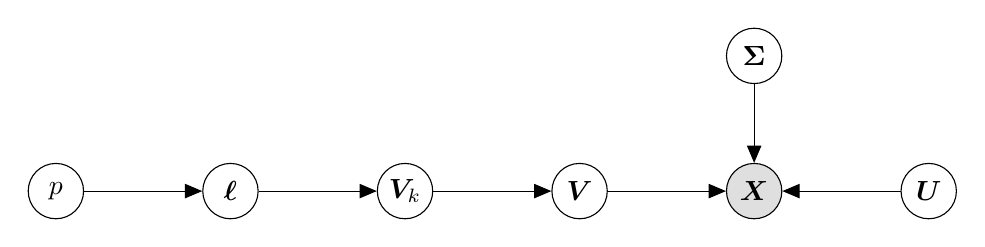
\begin{tikzpicture}

  % Define nodes
  \node[obs]                               (y) {$\bm{X}$};
  \node[latent, above=of y, xshift=0cm]  (x) {$\bm{\Sigma}$};
  \node[latent, right=1.5cm of y]            (w) {$\bm{U}$};
  \node[latent, left=1.5cm of y]            (V) {$\bm{V}$};
  \node[latent, left=1.5cm of V]            (Vk) {$\bm{V}_{k}$};
  \node[latent, left=1.5cm of Vk]            (l) {$\bm{\ell}$};
  \node[latent, left=1.5cm of l]            (p) {$p$};
  % Connect the nodes
  \edge {x,V,w} {y} ; %
  \edge {Vk} {V} ; %
  \edge {l} {Vk} ; %
  \edge {p} {l} ; %
  %\plate {} {(w)(y)(yx.north west)(yx.south west)} {$M$} ;

\end{tikzpicture}
% }


    % \caption{Visual description of the algorithm used to generate toy datasets
    % \label{f:matrix_generator_algorithm}
    % }
\caption{The pseudocode of the algorithm generating a matrix $\bm{X}$ with prescribed profile of $k$-leverage scores.}
\label{f:Matrix_Builder}
\end{figure}



\subsubsection{Volume sampling vs projection DPP}
This section sums up the results of numerical simulations on toy datasets. The number of observations is fixed to $N =100 $, the dimension to $d = 20$, and the number of selected columns to $k \in \{3,5\}$. Singular values are chosen from the following profiles: a spectrum with a cutoff called the projection spectrum,
$$
	\bm{\Sigma}_{k=3,\text{proj}} = 100 \sum\limits_{i = 1}^{3} \bm{e}_{i}\bm{e}_{i}^{\Tran} + 0.1 \sum\limits_{i = 4}^{20} \bm{e}_{i}\bm{e}_{i}^{\Tran}, $$
$$
	\bm{\Sigma}_{k=5,\text{proj}} = 100 \sum\limits_{i = 1}^{5} \bm{e}_{i}\bm{e}_{i}^{\Tran} + 0.1 \sum\limits_{i = 6}^{20} \bm{e}_{i}\bm{e}_{i}^{\Tran}. $$
a smooth spectrum
$$
	\bm{\Sigma}_{k=3,\text{smooth}} = 100\bm{e}_{1}\bm{e}_{1}^{\Tran} + 10\bm{e}_{2}\bm{e}_{2}^{\Tran} + \bm{e}_{3}\bm{e}_{3}^{\Tran} + 0.1 \sum\limits_{i = 4}^{20} \bm{e}_{i}\bm{e}_{i}^{\Tran},$$
$$
	\bm{\Sigma}_{k=5,\text{smooth}} = 10000\bm{e}_{1}\bm{e}_{1}^{\Tran} + 1000\bm{e}_{2}\bm{e}_{2}^{\Tran} + 100\bm{e}_{3}\bm{e}_{3}^{\Tran} +  10\bm{e}_{4}\bm{e}_{4}^{\Tran} +  \bm{e}_{5}\bm{e}_{5}^{\Tran} + 0.1 \sum\limits_{i = 6}^{20} \bm{e}_{i}\bm{e}_{i}^{\Tran},
	$$
\rev{and a flat spectrum with all singular values equal to $1$}
$$
\rev{    \bm{\Sigma}_{\text{identity}} = \sum\limits_{i = 1}^{20} \bm{e}_{i}\bm{e}_{i}^{\Tran}.}
    $$
Note that all profiles satisfy $\beta=1$; see \eqref{e:defbeta}. We discuss the case $\beta > 1$ at the end of the section. In each experiment, for each spectrum, we sample $200$ independent leverage score profiles that satisfy the sparsity constraints $p = \left| \{i \in [d], \bm{V}_{i,[k]} \neq \bm{0}\}\right|$ from a Dirichlet distribution of dimension $p$ with concentration parameter $1$ and equal means. For each leverage score profile, we sample a matrix $\bm{X}$ from the algorithm in Figure~\ref{f:Matrix_Builder}.
\begin{figure}
    \centering
\setcounter{subfigure}{0}%
\subfloat[$\bm{\Sigma}_{3,\text{proj}}$, $k=3$]{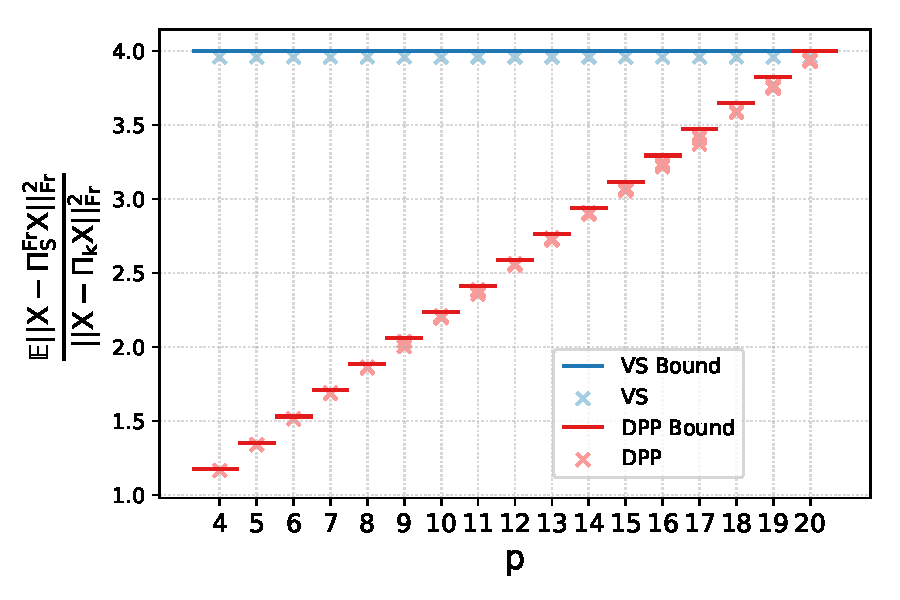
\includegraphics[width= 0.5\textwidth]{img/cssp/numexp/toydatasets/dpp_k_3_matrices_number_100_N_100_projection_spectrum_flat_spectrum_after}}
\setcounter{subfigure}{3}%
\subfloat[$\bm{\Sigma}_{5,\text{proj}}$, $k=5$]{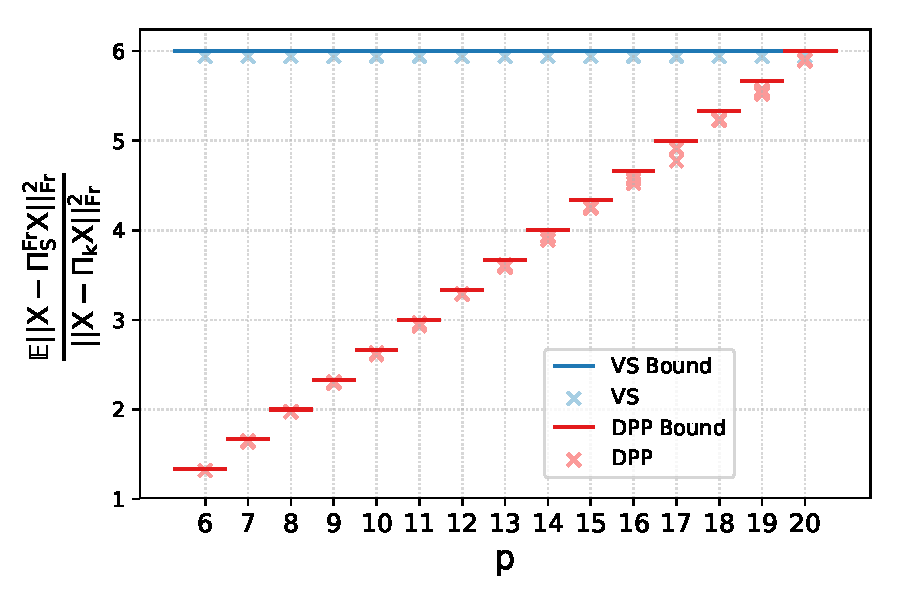
\includegraphics[width= 0.5\textwidth]{img/cssp/numexp/toydatasets/dpp_k_5_matrices_number_100_N_100_projection_spectrum_flat_spectrum_after}}\\
%\caption{The output of Algorithm \ref{algo_givens} for an input (k=2 d = 20)}
 %   \centering
 \setcounter{subfigure}{1}%
\subfloat[$\bm{\Sigma}_{3,\text{smooth}}$, $k=3$]{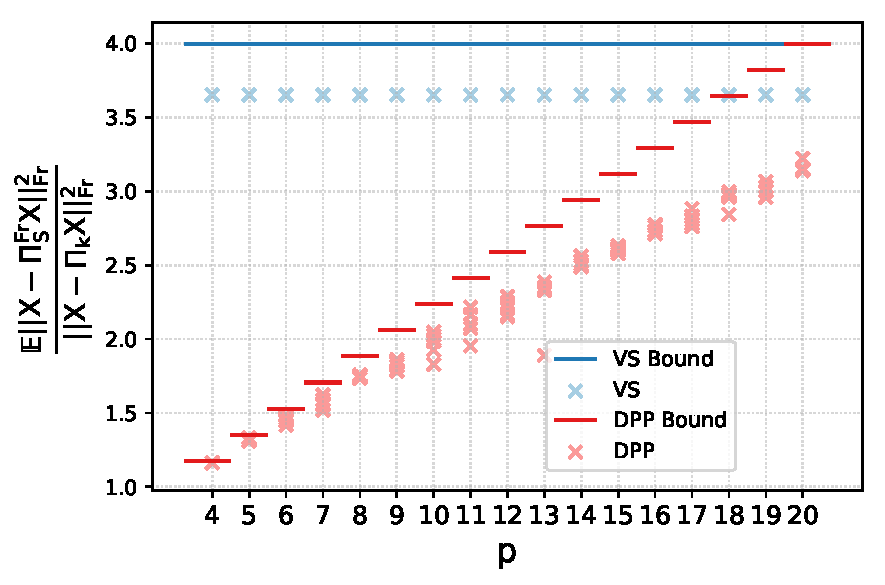
\includegraphics[width= 0.5\textwidth]{img/cssp/numexp/toydatasets/dpp_k_3_matrices_number_100_N_100_smooth_spectrum_flat_spectrum_after}}
\setcounter{subfigure}{4}%
\subfloat[$\bm{\Sigma}_{5,\text{smooth}}$, $k=5$]{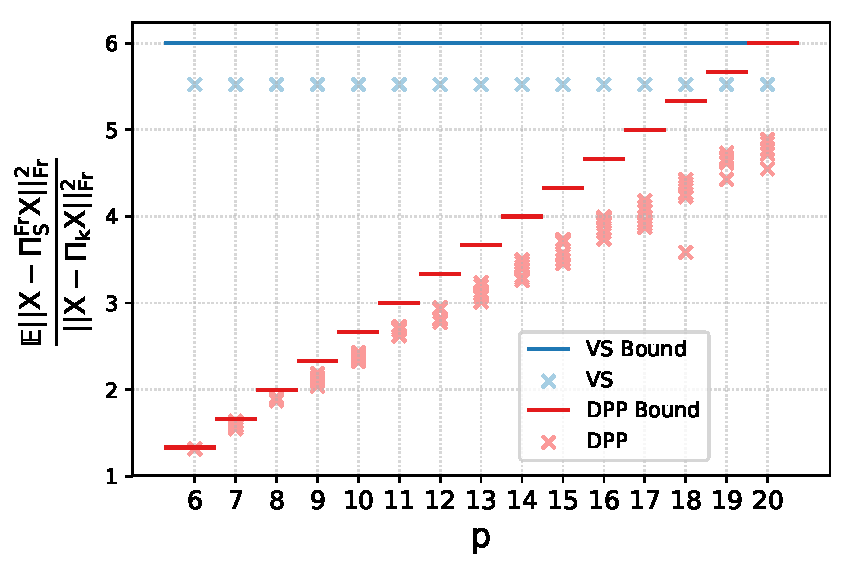
\includegraphics[width= 0.5\textwidth]{img/cssp/numexp/toydatasets/dpp_k_5_matrices_number_100_N_100_smooth_spectrum_flat_spectrum_after}}\\
 \setcounter{subfigure}{2}%
\subfloat[$\bm{\Sigma}_{\text{identity}}$, $k=3$]{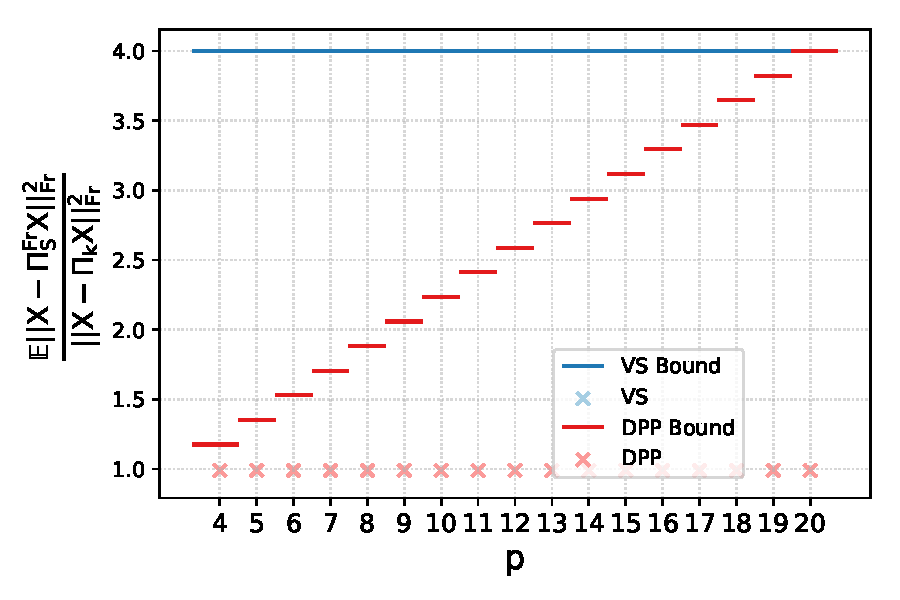
\includegraphics[width= 0.5\textwidth]{img/cssp/numexp/toydatasets/dpp_k_3_matrices_number_100_N_100_identity_spectrum_flat_spectrum_after}}
 \setcounter{subfigure}{5}%
\subfloat[$\bm{\Sigma}_{\text{identity}}$, $k=5$]{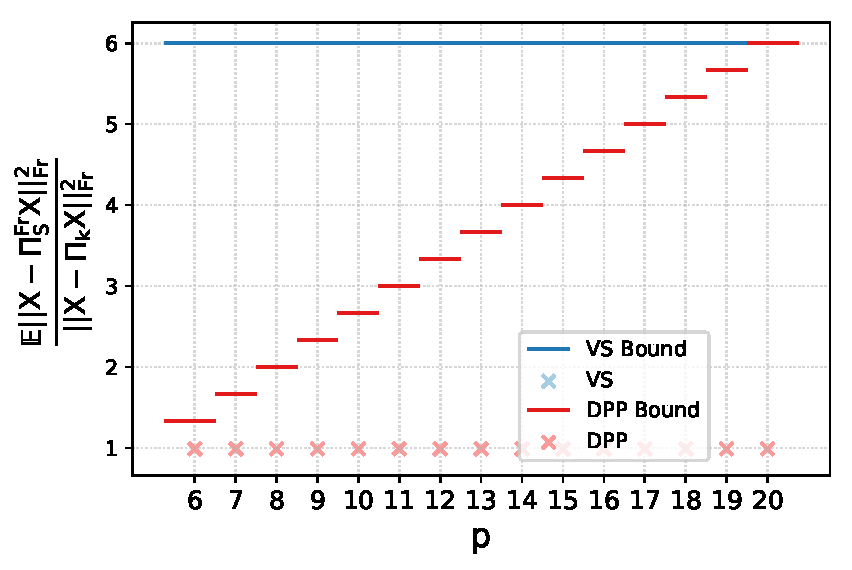
\includegraphics[width= 0.5\textwidth]{img/cssp/numexp/toydatasets/dpp_k_5_matrices_number_100_N_100_identity_spectrum_flat_spectrum_after}}

\caption{Realizations and bounds for $\mathbb{E} \|\bm{X}- \Pi_{S}^{\Fr} \bm{X}\|_{\Fr}^{2}$ as a function of the sparsity level $p$. \label{fig:toydatasets_vs_dpp_comparison_0}}
\end{figure}

%\paragraph{Volume sampling vs rejection projection DPP}

Figure~\ref{fig:toydatasets_vs_dpp_comparison_0} compares, on the one hand, the theoretical bounds in Theorem~\ref{thrm:volume_sampling_theorem} for volume sampling and Proposition~\ref{hypo_one_two_proposition} for the projection DPP, to the numerical evaluation of the expected error for sampled toy datasets on the other hand. The x-axis indicates various sparsity levels $p$. The unit on the $y$-axis is the error of PCA. There are 400 crosses on each subplot: each of the 200 matrices appears once for both algorithms. The 200 matrices are spread evenly across the values of $p$.

\rev{Used as a reference, the VS bounds are proportional to $(k+1)$ and independent of $p$. In fact, by Theorem~\ref{thm:schur_convex_volume_sampling}, the expected value of the Frobenius norm of the approximation error only depends on the spectrum of the matrix $\bm{X}$; in particular, it does not involve the matrix $\bm{V}$.} These bounds appear to be tight for projection spectra, and looser for smooth spectra.

For the projection DPP, the bound $1+k\frac{p-k}{d-k}$ is linear in $p$, and can thus be much lower than the bound of VS. The numerical evaluations of the error also suggest that this DPP bound is tight for a projection spectrum and looser in the smooth case. \rev{We emphasize that,} in both cases, the bound is representative of the actual behaviour of the algorithm.
%constantly badly
The bottom row of Figure~\ref{fig:toydatasets_vs_dpp_comparison_0} displays the same results for identity spectra, again for $k=3$ and $k=5$. This setting is extremely nonsparse and represents an arbitrarily bad scenario where even PCA would not make much practical sense. \rev{Then both} VS and DPP sampling perform \rev{the same as PCA}: all crosses superimpose at $y=1$. In this particular case, our linear bound in $p$ is not representative of the actual behaviour of the error. This observation can be explained for volume sampling using Theorem~\ref{thm:schur_convex_volume_sampling}, which states that the expected squared error under VS is Schur-concave, and is thus minimized for flat spectra. We have no similar result for the projection DPP.

Figure~\ref{fig:toydatasets_vs_dpp_comparison_1} provides a similar comparison for the two smooth spectra $\bm{\Sigma}_{3,\text{smooth}}$ and $\bm{\Sigma}_{5,\text{smooth}}$, but this time using the effective sparsity level $p_{\eff}(\theta)$ introduced in Theorem~\ref{prop:p_eff_proposition}. Qualitatively, we have observed the results to be robust to the choice of $\theta$\rev{: we use $\theta=2$}. The $200$ sampled matrices are now unevenly spread across the $x$-axis, since we do not control $p_{\eff}(\theta)$. Note finally that the DPP here is conditioned on the event $\{S \cap T_{p_{\mathrm{eff}}(\theta)}=\emptyset\}$, and sampled using an additional rejection sampling routine as detailed below Theorem~\ref{prop:p_eff_proposition}.

\begin{figure}
    \centering
\subfloat[$\bm{\Sigma}_{3,\text{smooth}}$]{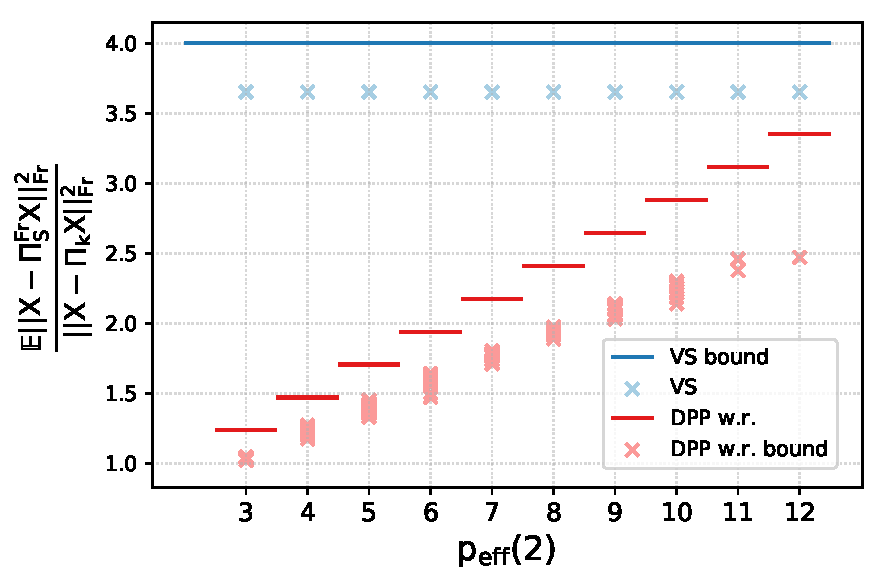
\includegraphics[width= 0.5\textwidth]{img/cssp/numexp/toydatasets/effective_kernel_k_3_matrices_number_100_N_100_smooth_spectrum_flat_spectrum_after}}
\subfloat[$\bm{\Sigma}_{5,\text{smooth}}$]{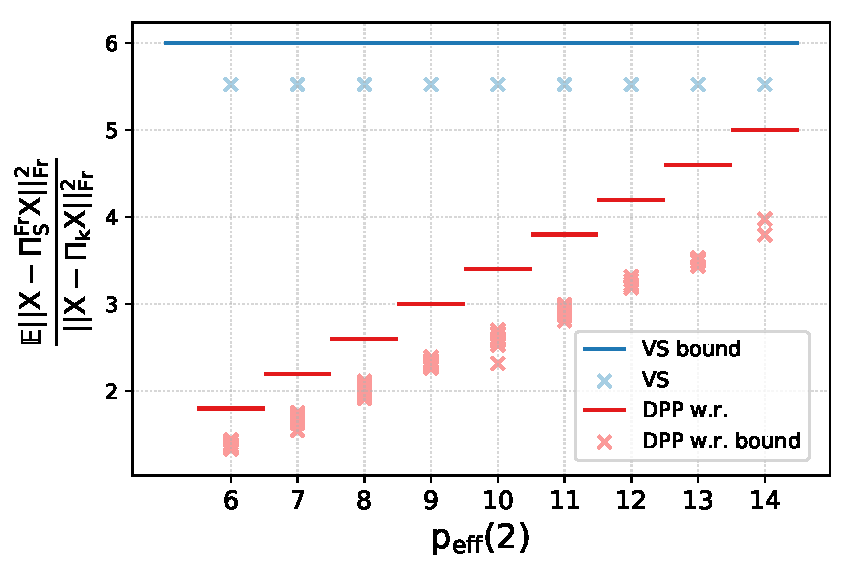
\includegraphics[width= 0.5\textwidth]{img/cssp/numexp/toydatasets/effective_kernel_k_5_matrices_number_100_N_100_smooth_spectrum_flat_spectrum_after}}\\

\caption{Realizations and bounds for $\mathbb{E} \|\bm{X}- \Pi_{S}^{\Fr} \bm{X}\|_{\Fr}^{2}$ as a function of the effective sparsity level $p_{\mathrm{eff}}(2)$.
\label{fig:toydatasets_vs_dpp_comparison_1}}
\end{figure}

\begin{figure}
    \centering
\subfloat[$\bm{\Sigma}_{3,\text{smooth}}$]{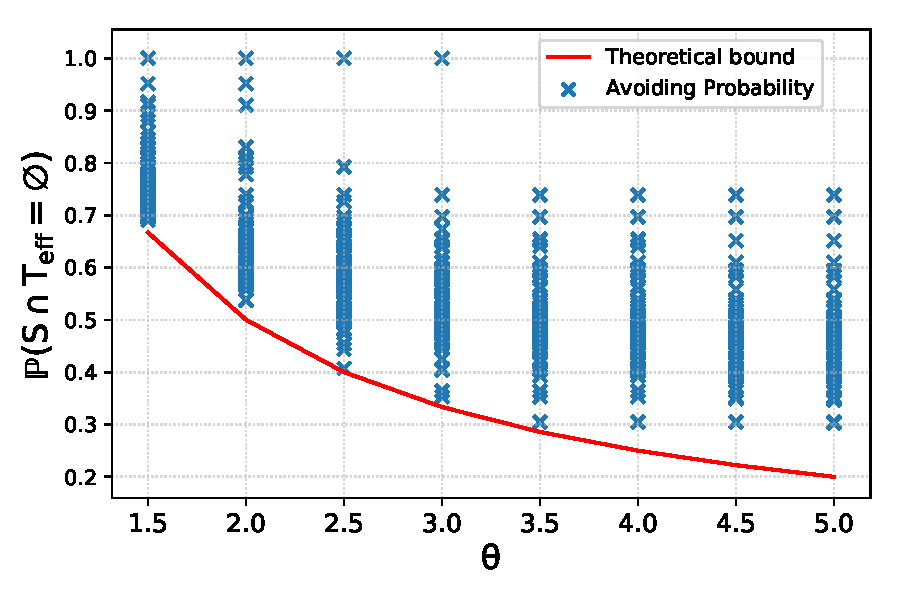
\includegraphics[width= 0.5\textwidth]{img/cssp/numexp/toydatasets/avoid_proba_k_3_matrices_number_100_N_100_smooth_spectrum_flat_spectrum_after}}
\subfloat[$\bm{\Sigma}_{5,\text{smooth}}$]{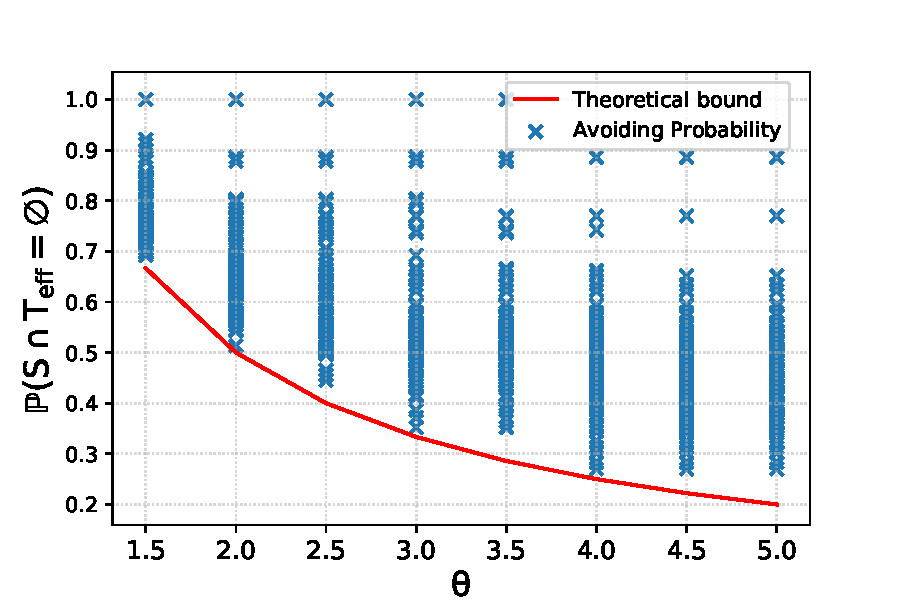
\includegraphics[width= 0.5\textwidth]{img/cssp/numexp/toydatasets/avoid_proba_k_5_matrices_number_100_N_100_smooth_spectrum_flat_spectrum_after}}\\

\caption{Realizations and bounds for the avoiding probability $\Prb(S \cap T_{p_{\mathrm{eff}}(\theta)} = \emptyset)$ in Theorem~\ref{prop:p_eff_proposition} as a function of $\theta$.
\label{fig:toydatasets_avoiding_proba}}
\end{figure}

For the DPP, the bound is again linear on the effective sparsity level $p_{\mathrm{eff}}(2)$, and can again be much lower than the VS bound. The behaviours of both VS and the projection DPP are similar to the exact sparsity setting of Figure~\ref{fig:toydatasets_vs_dpp_comparison_0}: the DPP has uniformly better bounds and actual errors, and the bound reflects the actual behaviour, relatively loosely when $p_{\eff}(2)$ is large.

Figure~\ref{fig:toydatasets_avoiding_proba} compares the theoretical bound in Theorem~\ref{prop:p_eff_proposition} for the avoiding probability $\Prb(S \cap T_{p_{\mathrm{eff}}(\theta)} = \emptyset)$ with 200 realizations, as a function of $\theta$. More precisely, we drew 200 matrices $\bm{X}$, and then for each $\bm{X}$, we computed exactly --~by enumeration~-- the value $\Prb(S \cap T_{p_{\mathrm{eff}}(\theta)} = \emptyset)$ for all values of $\theta$. The only randomness is thus in the sampling of $\bm{X}$, not the evaluation of the probability. \rev{Again, } the results suggest that the bound is relatively tight.

Finally, we examine relaxing $\beta=1$. We have observed our results to be robust with respect to $\beta$. At the extreme, in Figure~\ref{fig:toydatasets_vs_dpp_comparison_2}, we compare the errors for two additional spectra $\hat{\bm{\Sigma}}_{3,\text{proj}}$ and $\hat{\bm{\Sigma}}_{3,\text{smooth}}$ such that $\beta$ is close to its maximum value $d-k = 17$:

$$
    \hat{\bm{\Sigma}}_{k=3,\text{proj}} = 100 \sum\limits_{i = 1}^{3} \bm{e}_{i}\bm{e}_{i}^{\Tran} + 0.1\bm{e}_{4}^{\phantom{\Tran}}\bm{e}_{4}^{\Tran} + 10^{-4} \sum\limits_{i = 5}^{20} \bm{e}_{i}^{\phantom{\Tran}}\bm{e}_{i}^{\Tran}, $$
and
$$
    \hat{\bm{\Sigma}}_{k=3,\text{smooth}} = 100\bm{e}_{1}\bm{e}_{1}^{\Tran} + 10\bm{e}_{2}\bm{e}_{2}^{\Tran} + \bm{e}_{3}\bm{e}_{3}^{\Tran} + 0.1\bm{e}_{4}^{\phantom{\Tran}}\bm{e}_{4}^{\Tran} + 10^{-4} \sum\limits_{i = 5}^{20} \bm{e}_{i}^{\phantom{\Tran}}\bm{e}_{i}^{\Tran}.$$
 While the bound for such a large $\beta$ \rev{would be} almost vertical and does not reflect anymore the actual behaviour of the algorithm, we observe that the algorithm still performs comparably to the setting where $\beta=1$, although with more variance, and that the bound with $\beta = 1$ (in red) still represents the behaviour of the algorithm. This is a hint that there is room for improvement in our bounds in the large $\beta$ regime. The search for a new bound that would be independent of $\beta$ is nontrivial and a subject of future work.
% =======
% Figure~\ref{fig:toydatasets_vs_dpp_comparison_2} provides a similar comparison for two spectra $\hat{\bm{\Sigma}}_{3,\text{proj}}$ and $\hat{\bm{\Sigma}}_{3,\text{smooth}}$ in the case $\beta$ is large:

% $$
%     \hat{\bm{\Sigma}}_{k=3,\text{proj}} = 100 \sum\limits_{i = 1}^{3} \bm{e}_{i}\bm{e}_{i}^{\Tran} + 0.1 \sum\limits_{i = 4}^{6} \bm{e}_{i}\bm{e}_{i}^{\Tran} + 0.0001 \sum\limits_{i = 7}^{20} \bm{e}_{i}\bm{e}_{i}^{\Tran}, $$
% and
% $$
%     \hat{\bm{\Sigma}}_{k=3,\text{smooth}} = 100\bm{e}_{1}\bm{e}_{1}^{\Tran} + 10\bm{e}_{2}\bm{e}_{2}^{\Tran} + \bm{e}_{3}\bm{e}_{3}^{\Tran} +  0.1 \sum\limits_{i = 4}^{6} \bm{e}_{i}\bm{e}_{i}^{\Tran} + 0.0001 \sum\limits_{i = 7}^{20} \bm{e}_{i}\bm{e}_{i}^{\Tran} .$$
% We observe that even for a large value of $\beta$, the approximations errors are close to our theoretical bound when $\beta = 1$.
% >>>>>>> dd22764e45ee3cf349672d30378fcd247ab4c3c7
\begin{figure}
    \centering
%\caption{The output of Algorithm \ref{algo_givens} for an input (k=2 d = 20)}
 %   \centering
% \setcounter{subfigure}{1}%
% \subfloat[$\hat{\bm{\Sigma}}_{3,\text{proj}}$, $k=3$]{\includegraphics[width= 0.5\textwidth]{img/numexp/toydatasets/purple_beta_larger_than_one/dpp_k_3_matrices_number_500_N_100_projection_spectrum_flat_spectrum_after}}
% \subfloat[$\hat{\bm{\Sigma}}_{3,\text{smooth}}$, $k=3$]{\includegraphics[width= 0.5\textwidth]{img/numexp/toydatasets/purple_beta_larger_than_one/dpp_k_3_matrices_number_500_N_100_smooth_spectrum_flat_spectrum_after}}


\subfloat[$\hat{\bm{\Sigma}}_{3,\text{smooth}}$, $k=3$]{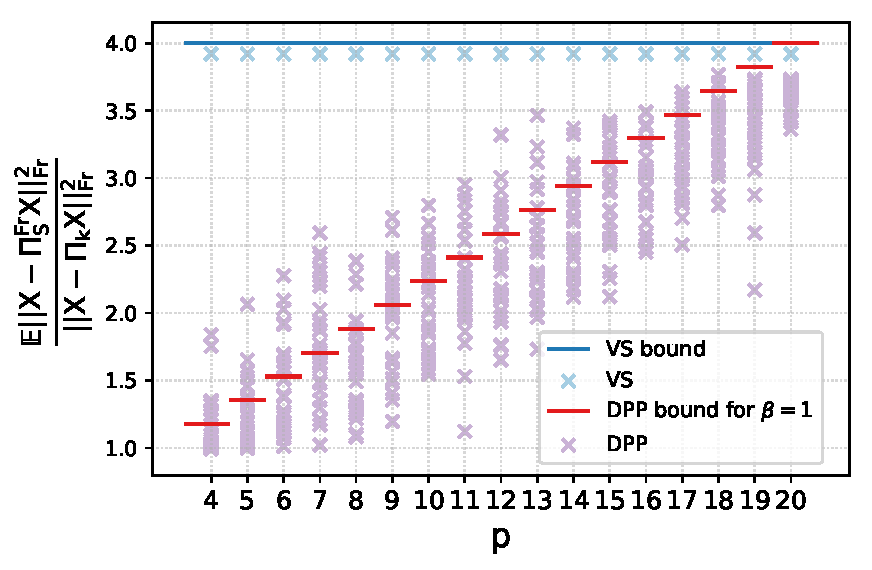
\includegraphics[width= 0.5\textwidth]{img/cssp/numexp/toydatasets/dpp_k_3_matrices_number_500_N_100_smooth_spectrum_flat_spectrum_after_beta_large}}
\subfloat[$\hat{\bm{\Sigma}}_{3,\text{proj}}$, $k=3$]{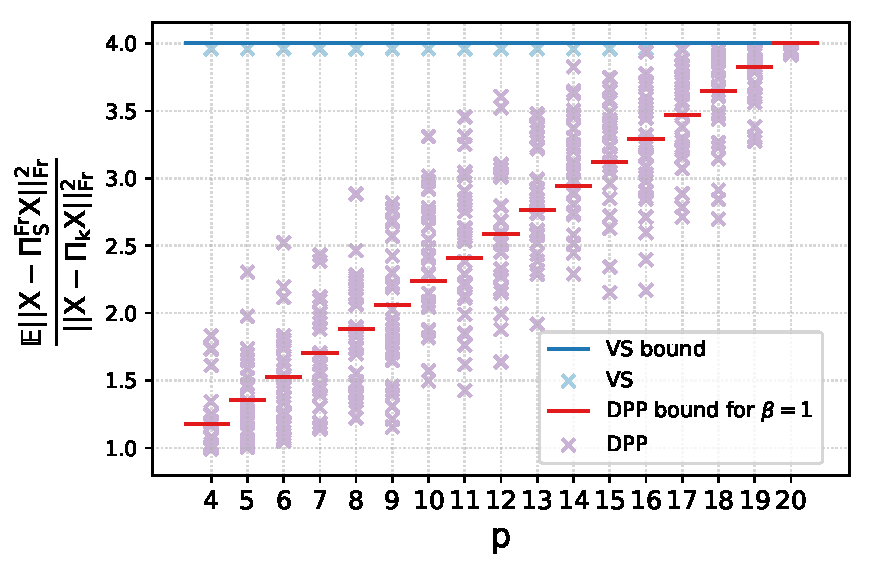
\includegraphics[width= 0.5\textwidth]{img/cssp/numexp/toydatasets/dpp_k_3_matrices_number_500_N_100_projection_spectrum_flat_spectrum_after_beta_large}}
%\setcounter{subfigure}{3}%

\caption{Realizations and bounds for $\mathbb{E} \|\bm{X}- \Pi_{S}^{\Fr} \bm{X}\|_{\Fr}^{2}$ as a function of the sparsity level $p$ in the case $\beta >1$. \label{fig:toydatasets_vs_dpp_comparison_2}}
\end{figure}

% Figure~\ref{fig:toydatasets_vs_dpp_comparison_3} compares the theoretical bound with the numerical evaluations for the volume sampling and the projection DPP for different levels of "smoothness" of the spectrum. Theoretical bounds are sharp for the projection spectrum matrices (subfigures (a) and (b)), while they become loose for smooth spectrum matrices (subfigures (c) and (d)) and in the extreme case of the flat spectrum of identity matrix (subfigures (e) and (f)).
% Figure~\ref{fig:toydatasets_vs_dpp_comparison_3} compares the theoretical bound with the numerical evaluations for the volume sampling and the projection DPP for several  with the numerical evaluations for the avoiding probability $\Prb(S \cap T_{p_{\mathrm{eff}}(\theta)} = \emptyset)$ as a function of $\theta$ for the projection DPP. The theoretical bound $\frac{1}{\theta}$, see Proposition~\ref{hypo_one_two_proposition}, is verified, moreover our numerical simulations suggest that this bound is tight.


%\paragraph{Relaxing the hypothesis $N \geq d$}


% \begin{figure}
%     \centering
%         \centering
% 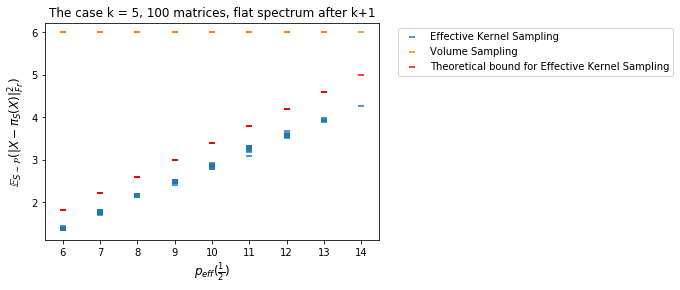
\includegraphics[width= 0.9\textwidth]{img/numexp/toydatasets/k_5-spectrum-hyp-valid_100matrices_effectivekernel_projectionspectrum.png}
%     \caption{Volume sampling vs effective kernel
%     }
% \end{figure}


% \begin{figure}
%     \centering
%         \centering
% 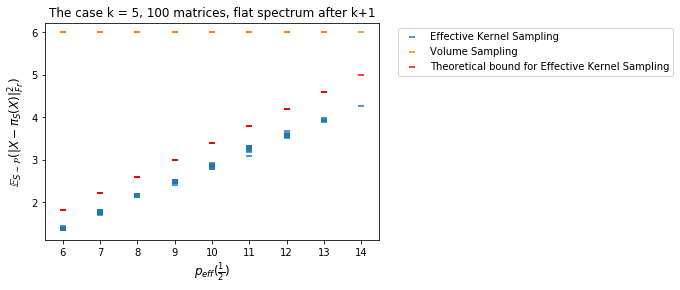
\includegraphics[width= 0.9\textwidth]{img/numexp/toydatasets/k_5-spectrum-hyp-valid_100matrices_effectivekernel_projectionspectrum.png}
%     \caption{Volume sampling vs effective kernel
%     }
% \end{figure}


% \begin{figure}
%     \centering
%         \centering
% 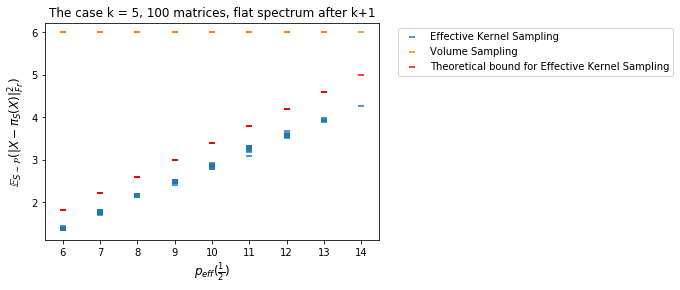
\includegraphics[width= 0.9\textwidth]{img/numexp/toydatasets/k_5-spectrum-hyp-valid_100matrices_effectivekernel_projectionspectrum.png}
%     \caption{Volume sampling vs effective kernel
%     }
% \end{figure}



% \begin{figure}
%     \centering
%         \centering
% 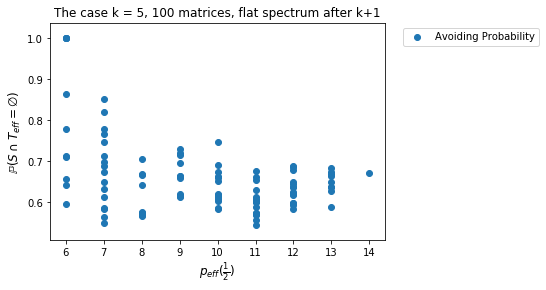
\includegraphics[width= 0.9\textwidth]{img/numexp/toydatasets/k_5-spectrum-hyp-valid_100matrices_rejectionproba_allcardinals_projectionspectrum.png}
%     \caption{Avoiding probability for the effective kernel
%     }
% \end{figure}

% \begin{figure}
%     \centering
%         \centering
% 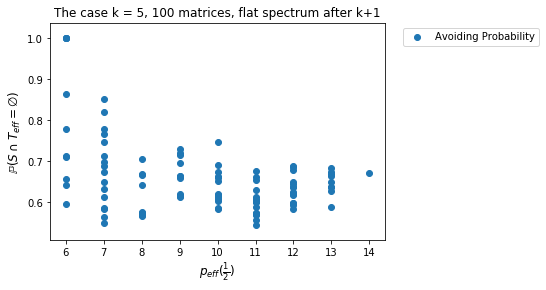
\includegraphics[width= 0.9\textwidth]{img/numexp/toydatasets/k_5-spectrum-hyp-valid_100matrices_rejectionproba_allcardinals_projectionspectrum.png}
%     \caption{Avoiding probability for the effective kernel
%     }
% \end{figure}

% \begin{figure}
%     \centering
%         \centering
% 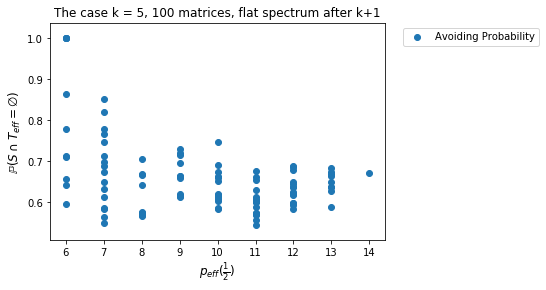
\includegraphics[width= 0.9\textwidth]{img/numexp/toydatasets/k_5-spectrum-hyp-valid_100matrices_rejectionproba_allcardinals_projectionspectrum.png}
%     \caption{Avoiding probability for the effective kernel
%     }
% \end{figure}

\subsection{Real datasets}
\label{s:realDatasets}
%\paragraph{Datasets with extreme sparsity of $k$-leverage scores}

\begin{table}[h]
\centering
 \begin{tabular}{| c| c | c| c|}
 \hline
  Dataset & Application domain & $N \times d$  &  References\\
 \hline
 Colon & genomics & $62 \times 2000$  & \citep{Al99}\\
 \hline
 Leukemia & genomics &$72 \times 7129$ & \citep{Go99}\\
 \hline
 Basehock & text processing &$1993 \times 4862$ & \citep{Li17} \\
 \hline
 Relathe & text processing & $1427 \times 4322$ & \citep{Li17}\\
 \hline
\end{tabular}
\caption{Datasets used in the experimental section.
\label{table:real_datasets}}
\end{table}

%This section compares the empirical performances of several column subset selection algorithms on the datasets in Table~\ref{table:real_datasets}.
\rev{The datasets described in Table~\ref{table:real_datasets}} are illustrative of two extreme situations regarding the sparsity of the $k$-leverage scores. For instance, the dataset Basehock has a very sparse profile of $k$-leverage scores, while the dataset Colon has a quasi-uniform distribution of $k$-leverage scores, see Figures~\ref{subfig:basehock_cumul_klv}  \& \ref{subfig:colon_cumul_klv}. \rev{This section compares the empirical performances of several column subset selection algorithms on these datasets.}

We consider the following algorithms presented in Section~\ref{s:relatedwork}: 1) the projection DPP with marginal kernel $\bm{K}=\bm{V}_{k}^{}\bm{V}_{k}^{\Tran}$, 2) volume sampling, using the implementation proposed by \cite{KuTa11}, 3) deterministically picking the largest $k$-leverage scores, 4) pivoted QR as in \cite{Golu65}, although the only known bounds for this algorithm are for the spectral norm, and 5) double phase, with $c$ manually tuned to optimize the performance, usually around $c \approx 10k$.

%Comments on fig 7
The rest of Figure~\ref{fig:colon_vs_basehock_comparison} sums up the empirical results of these algorithms on the Colon and Basehock datasets.
%
Figures~\ref{subfig:basehock_all_algos} \& \ref{subfig:colon_all_algos} illustrate the results of the five algorithms in the following setting. An ensemble of 50 subsets are sampled using each algorithm. We give the corresponding boxplots for the Frobenius errors, on Colon and Basehock respectively.
%
Deterministic methods (largest leverage scores and pivoted QR) perform well compared with other algorithms on the Basehock dataset; in contrast, they display very bad performance on the Colon dataset.

Focusing now on the three random sampling methods, we first make sure that the observed differences in Frobenius error are statistically significant at level $\alpha=0.05$. To that end, we report in Table~\ref{t:tests} the $p$-values of the three pairwise Mann-Whitney tests between the three algorithms. More precisely, let $F_\text{X}$ denote the CDF of the Frobenius errors for algorithm $\text{X}\in\{\DPh,\DPP,\VS\}$. We test $H_0$:``$F_\text{X}=F_\text{Y}$" against the so-called \emph{one-sided} alternative $H_1$ that X is better than Y, in the sense that if you independently run algorithms X and Y, it is more likely that the Frobenius error of X is the smaller of the two. Now, we want to \emph{jointly} test whether all three pairs of algorithms within $\{\DPh,\DPP,\VS\}$ perform differently, so we use a Bonferroni correction \citep{Was13}. Looking at Table~\ref{t:tests} for dataset Colon, all three $p$-values are smaller than $\alpha/3=0.05/3$, so that we simultaneously reject that $F_{\DPh}=F_{\DPP}$, $F_{\DPh}=F_{\VS}$ and $F_{\DPP}=F_{\VS}$, and we declare the differences among algorithms to be statistically significant. The same can be said for dataset Basehock. In particular, we observe that the increase in performance using the projection DPP compared to volume sampling is more important for the Basehock dataset than for the Colon dataset: this improvement can be explained by the sparsity of the $k$-leverage scores as predicted by our approximation bounds.
%
The double phase algorithm has the best results on both datasets. However its theoretical guarantees cannot predict such an improvement, as noted in Section~\ref{s:relatedwork}. The performance of the projection DPP is comparable to double phase and makes it a close second, with a slightly larger gap on the Colon dataset. We emphasize that our approximation bounds are sharp compared to numerical observations.

%%%% Boosting Fig 7
Figures~\ref{subfig:basehock_all_algos_boosting} \& \ref{subfig:colon_all_algos_boosting} show results obtained using a classical boosting technique for randomized algorithms. \rev{We repeat 20 times the following procedure: sample 50 subsets $(S_{i})_{i \in [50]}$ and take the subset $S_{\min}$ that minimizes the approximation error among the elements of the batch $(S_{i})_{i \in [50]}$}. Displayed boxplots are for these 20 best results. The same comparisons apply as without boosting, with $p$-values given in Table~\ref{t:tests_boosted}.

%%% Figure 7
\begin{figure}
    \centering
    \captionsetup[subfigure]{justification=centering}
\subfloat[$k$-leverage scores profile and cumulative profile for the dataset Basehock (k=10).]{\includegraphics[width= 0.5\textwidth, height = 0.2\textheight]{img/cssp/numexp/realdatasets/BASEHOCK_cumul_klv_k_10.pdf}\label{subfig:basehock_cumul_klv}}~
\subfloat[$k$-leverage scores profile and cumulative profile for the dataset Colon (k=10).]{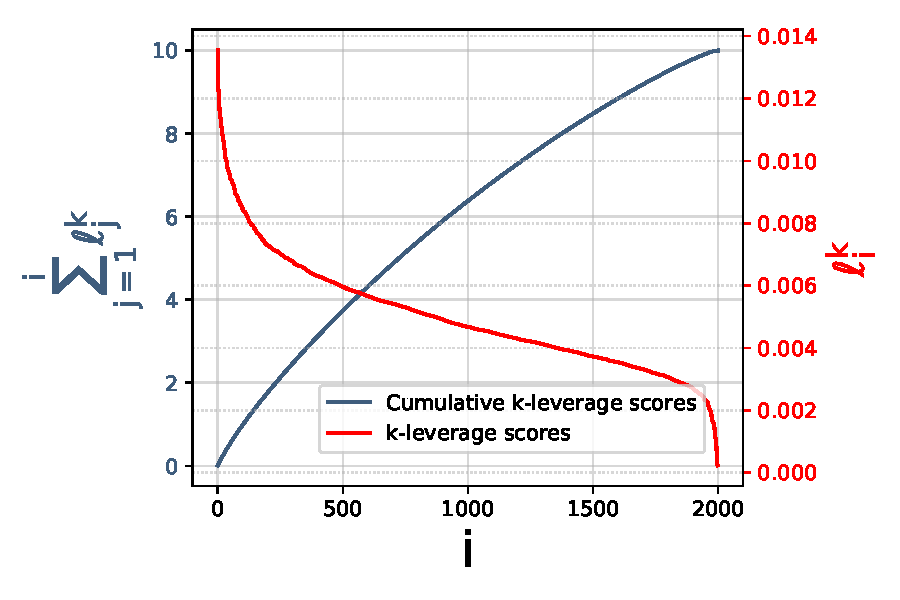
\includegraphics[width= 0.5\textwidth, height = 0.2\textheight]{img/cssp/numexp/realdatasets/colon_cumul_klv_k_10.pdf}\label{subfig:colon_cumul_klv}}\\
%\caption{The output of Algorithm \ref{algo_givens} for an input (k=2 d = 20)}
 %   \centering
\subfloat[Boxplots of $\|\bm{X}-\Pi_{S}^{\Fr}\bm{X}\|_{\Fr}$ on a batch of 50 samples for the five algorithms on the dataset Basehock (k=10).]{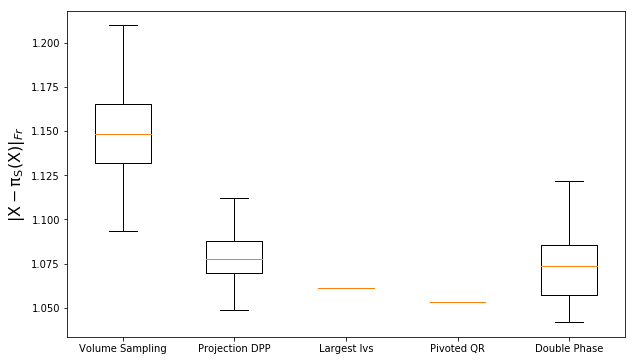
\includegraphics[width= 0.5\textwidth]{img/cssp/numexp/realdatasets/BASEHOCK_allalgos_50samples_k_10.pdf}\label{subfig:basehock_all_algos}}~
\subfloat[Boxplots of $\|\bm{X}-\Pi_{S}^{\Fr}\bm{X}\|_{\Fr}$ on a batch of 50 samples for the five algorithms on the dataset Colon (k=10).]{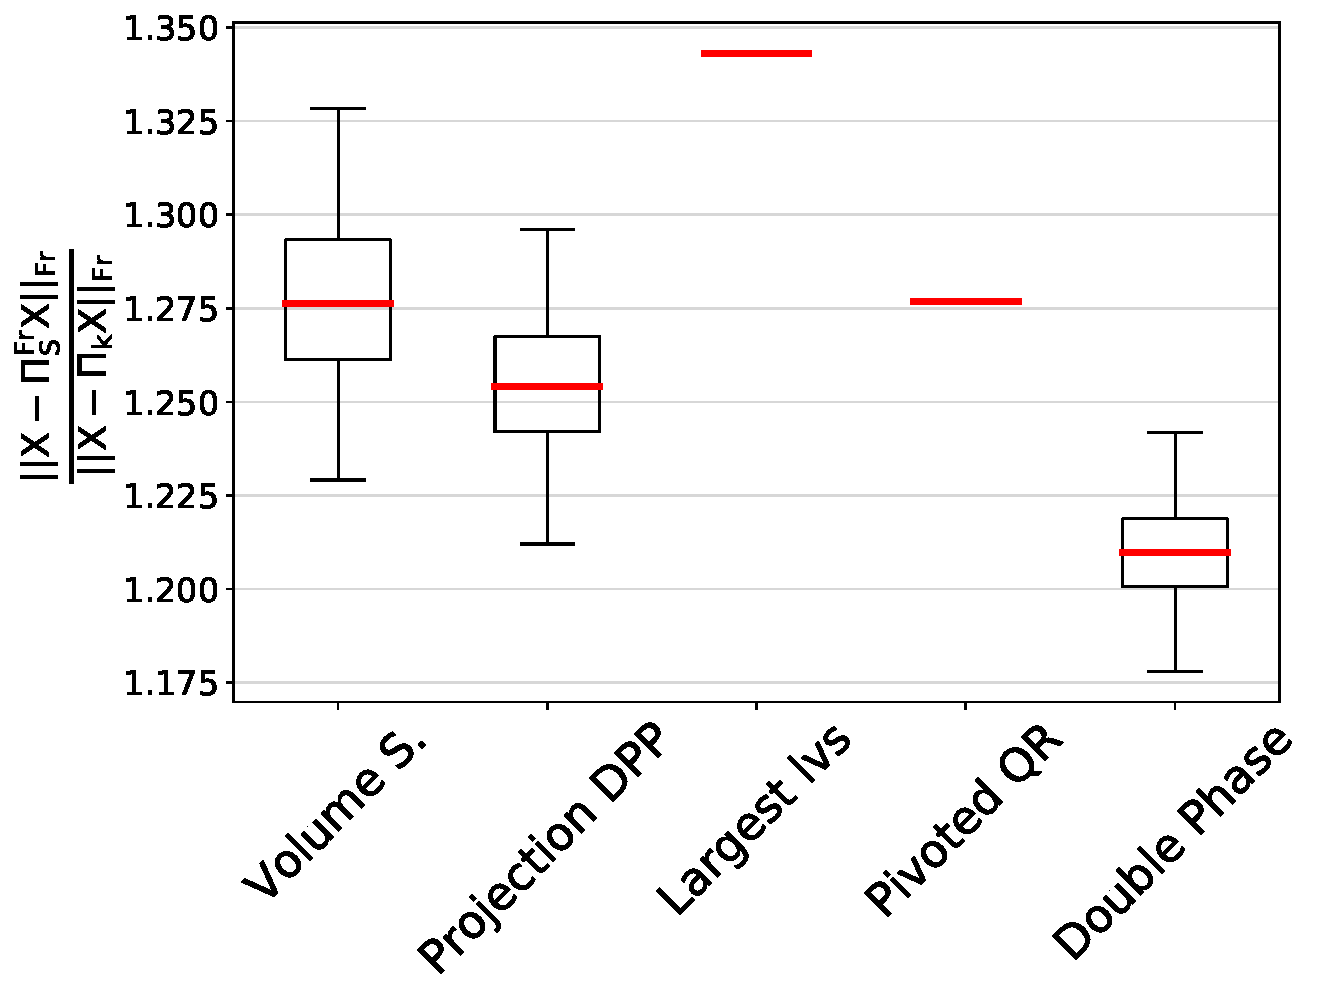
\includegraphics[width= 0.5\textwidth]{img/cssp/numexp/realdatasets/colon_allalgos_50samples_k_10.pdf}\label{subfig:colon_all_algos}}\\
\subfloat[Boxplots of $\|\bm{X}-\Pi_{S}^{\Fr}\bm{X}\|_{\Fr}$ on a batch of 50 samples for the boosting of randomized algorithms on the dataset Basehock (k=10).]{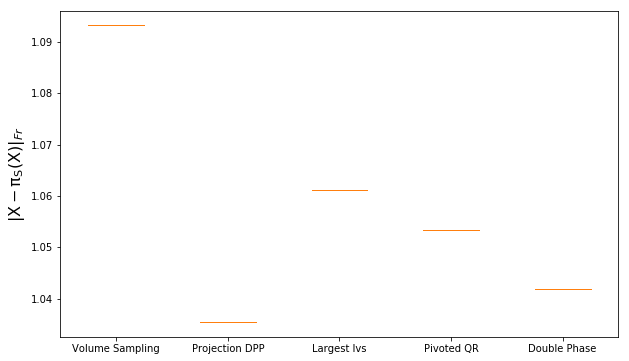
\includegraphics[width= 0.5\textwidth]{img/cssp/numexp/realdatasets/BASEHOCK_boosting_allalgos_50samples_k_10.pdf}\label{subfig:basehock_all_algos_boosting}}~
\subfloat[Boxplots of $\|\bm{X}-\Pi_{S}^{\Fr}\bm{X}\|_{\Fr}$ on a batch of 50 samples for the boosting of randomized algorithms on the dataset Colon (k=10).]{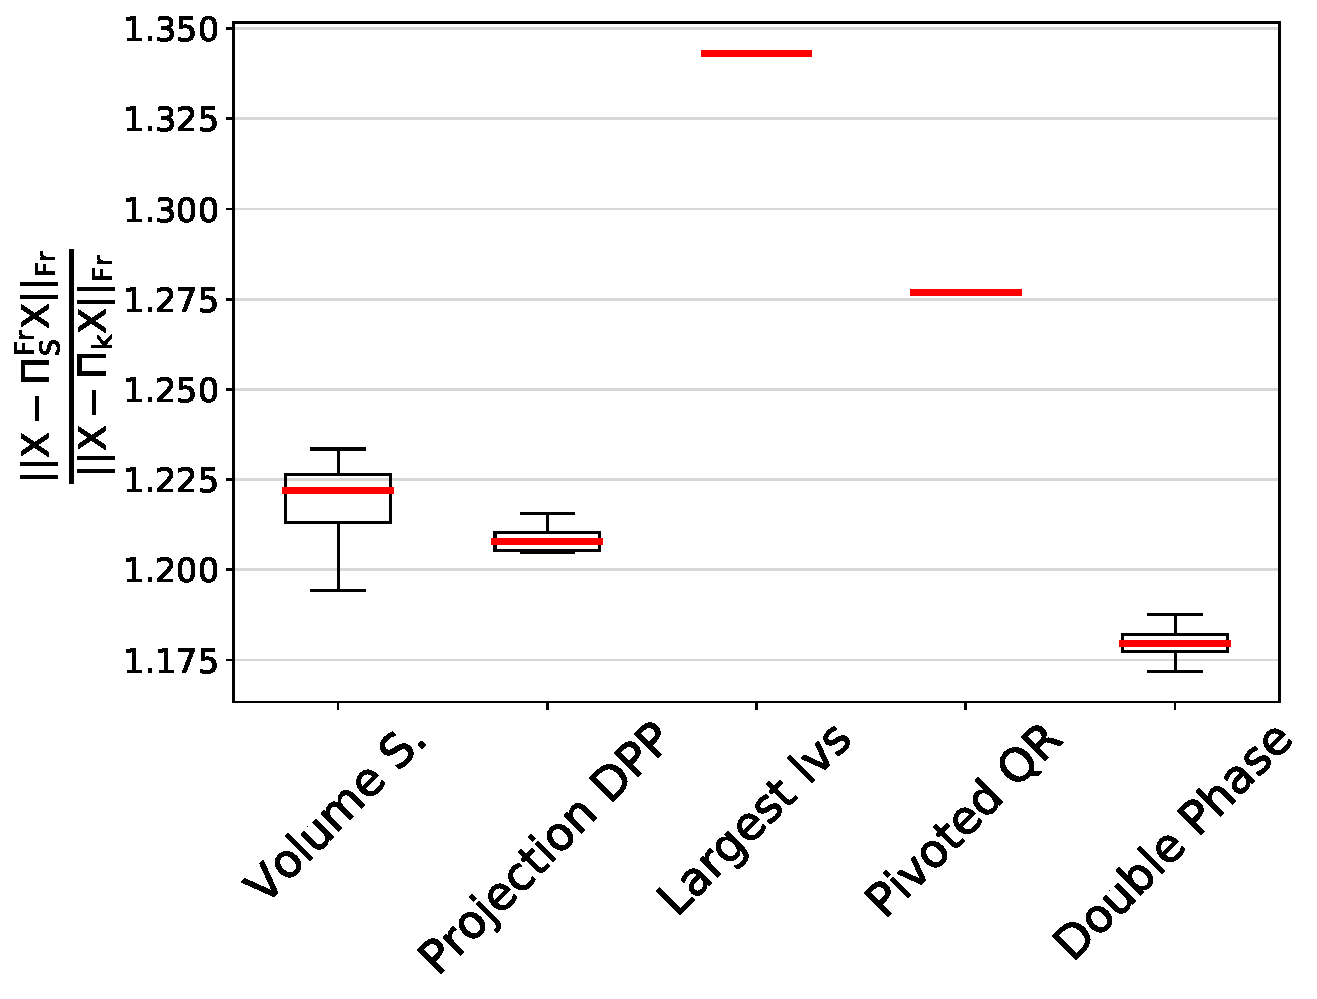
\includegraphics[width= 0.5\textwidth]{img/cssp/numexp/realdatasets/colon_boosting_allalgos_50samples_k_10.pdf}\label{subfig:colon_all_algos_boosting}}\\
\caption{Comparison of several column subset selection algorithms for two datasets \rev{with different leverage score profiles}: Basehock and Colon.\label{fig:colon_vs_basehock_comparison}}
\end{figure}

%%%%%%%%%%% Comment on Fig 8  => tout après Fig. 7.
Figure~\ref{fig:leukemia_vs_relathe_comparison} calls again for similar comments, comparing this time the datasets Relathe (with concentrated profile of $k$-leverage scores) and Leukemia (with almost uniform profile of $k$-leverage scores). This time, the same test as for Colon vs. Basehock in Table~\ref{t:tests} further reveals that we cannot reject the hypothesis that $F_{\DPh}=F_{\DPP}$ on Relathe. In other words, there is no hint that \rev{the performance of the double phase is different from that of DPP} on that particular dataset \rev{(at level $\alpha=0.05$)}. The same is true for the boosted version of the algorithms; see Table~\ref{t:tests_boosted}.

\begin{figure}
    \centering
    \captionsetup[subfigure]{justification=centering}
\subfloat[$k$-leverage scores profile and cumulative profile for the dataset Relathe (k=10).]{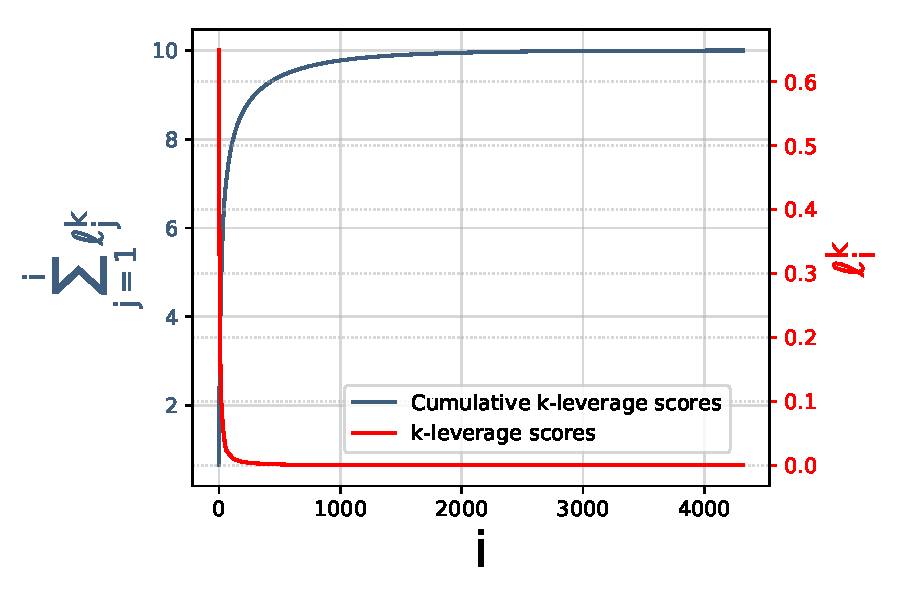
\includegraphics[width= 0.5\textwidth, height = 0.2\textheight]{img/cssp/numexp/realdatasets/RELATHE_cumul_klv_k_10.pdf}}~
\subfloat[$k$-leverage scores profile and cumulative profile for the dataset Leukemia (k=10).]{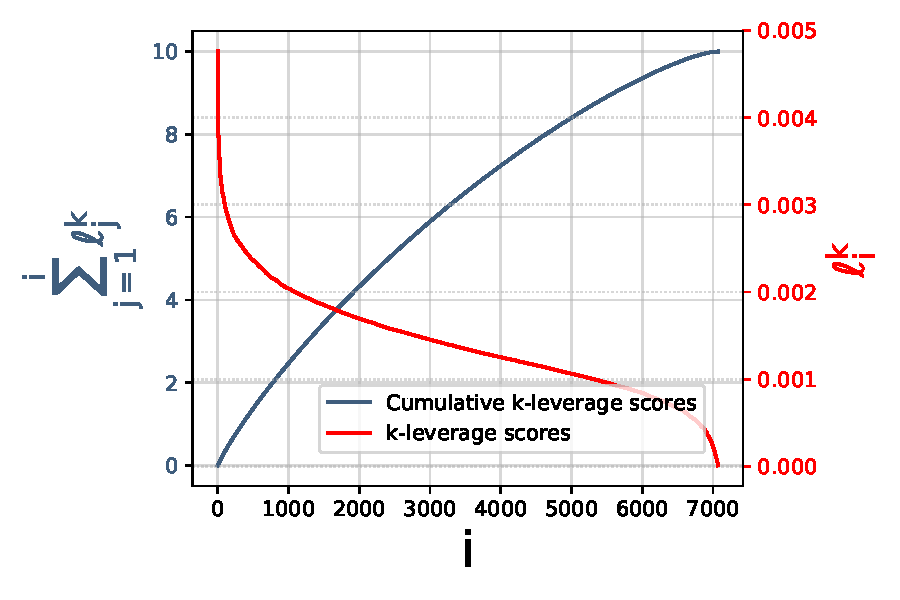
\includegraphics[width= 0.5\textwidth, height = 0.2\textheight]{img/cssp/numexp/realdatasets/leukemia_cumul_klv_k_10.pdf}}\\
%\caption{The output of Algorithm \ref{algo_givens} for an input (k=2 d = 20)}
 %   \centering
\subfloat[Boxplots of $\|\bm{X}-\Pi_{S}^{\Fr}\bm{X}\|_{\Fr}$ on a batch of 50 samples for the five algorithms on the dataset Relathe (k=10).]{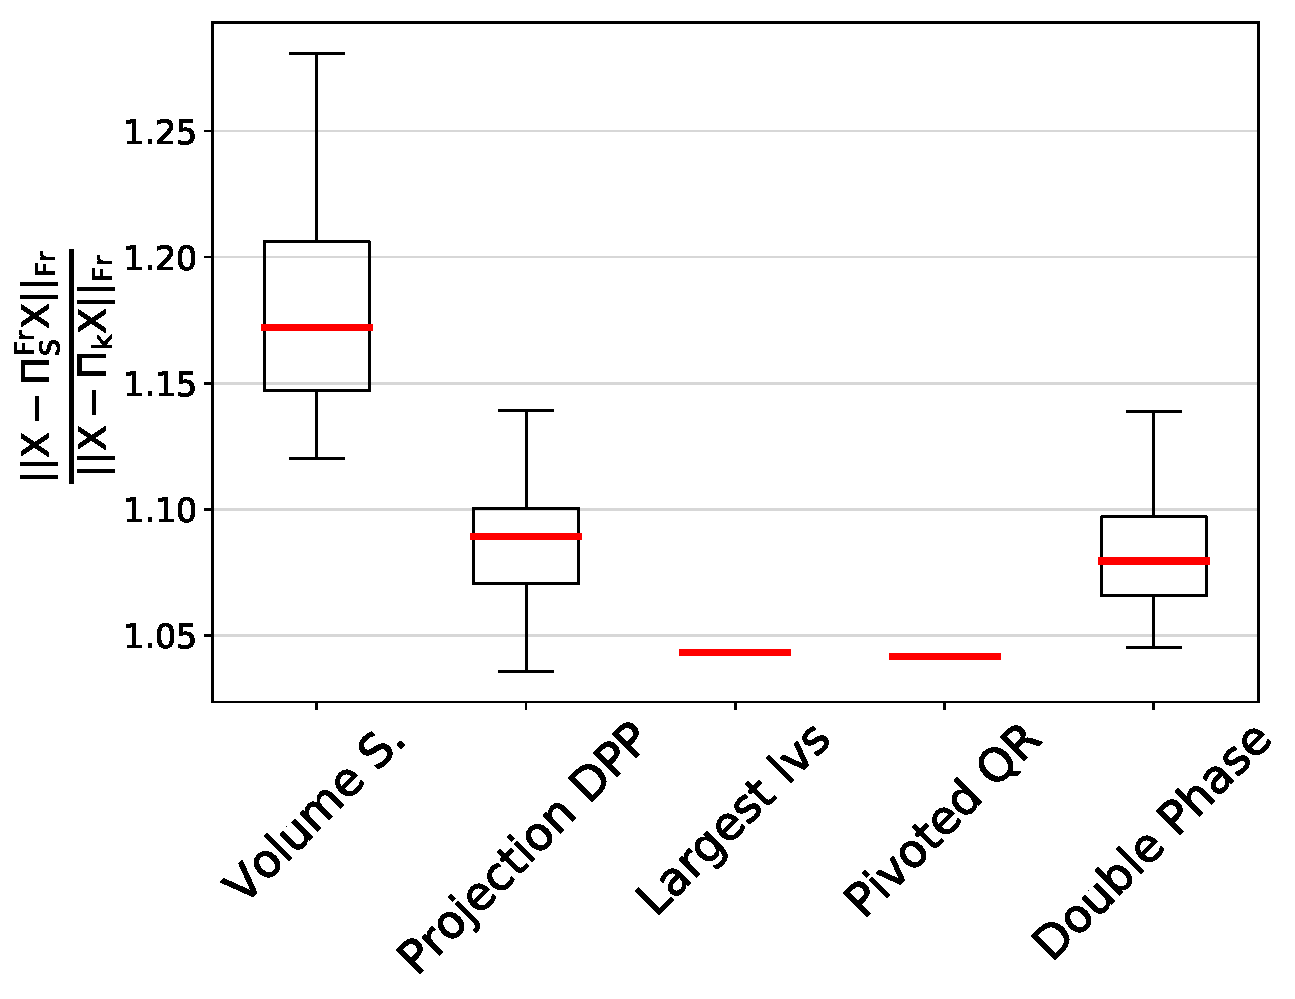
\includegraphics[width= 0.5\textwidth]{img/cssp/numexp/realdatasets/RELATHE_allalgos_50samples_k_10.pdf}}~
\subfloat[Boxplots of $\|\bm{X}-\Pi_{S}^{\Fr}\bm{X}\|_{\Fr}$ on a batch of 50 samples for the five algorithms on the dataset Leukemia (k=10).]{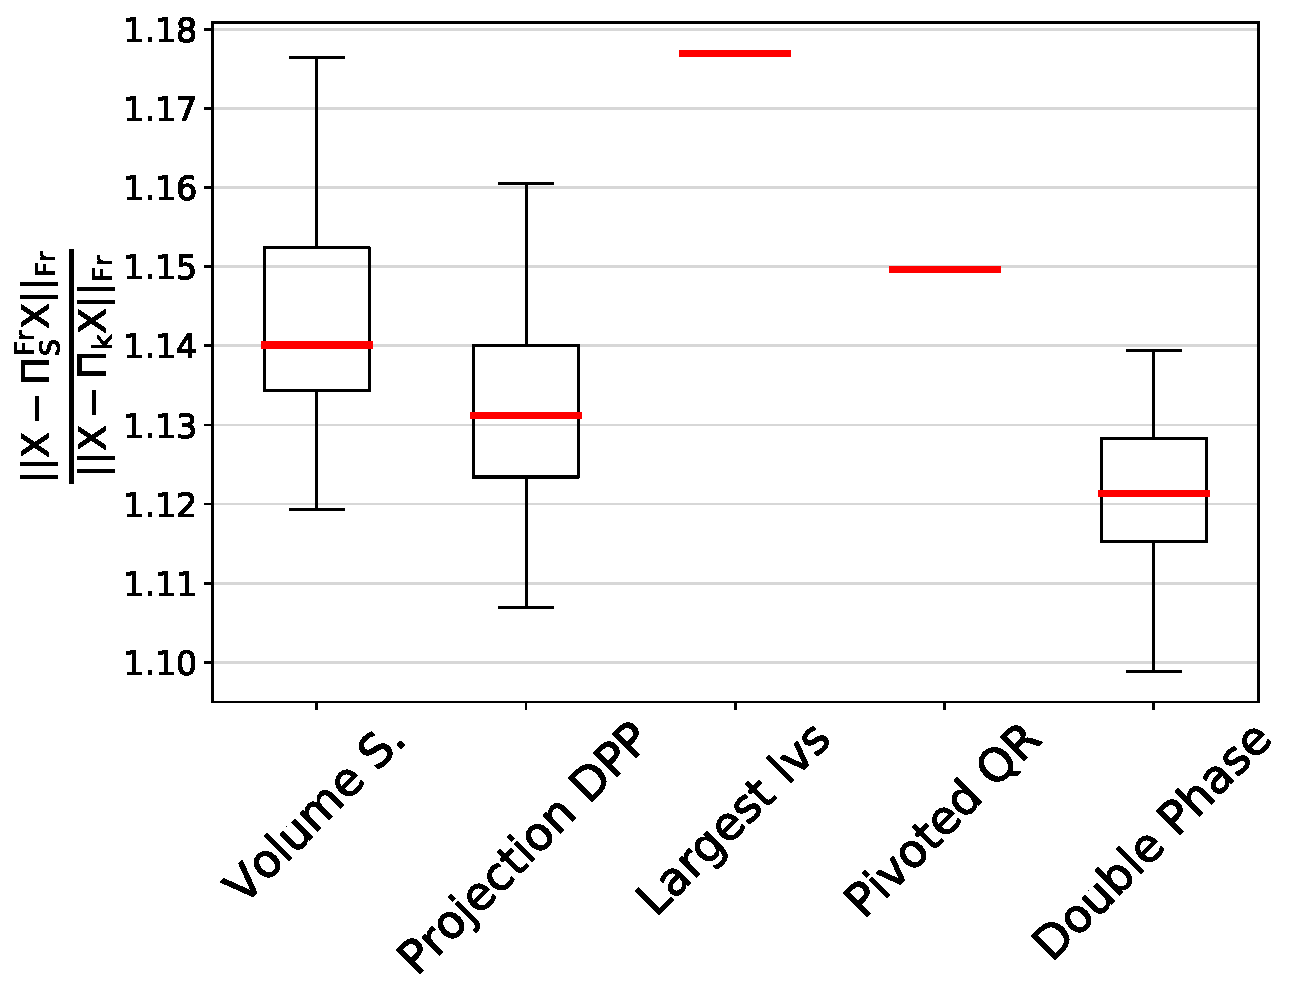
\includegraphics[width= 0.5\textwidth, ]{img/cssp/numexp/realdatasets/leukemia_allalgos_50samples_k_10.pdf}}\\
\subfloat[Boxplots of $\|\bm{X}-\Pi_{S}^{\Fr}\bm{X}\|_{\Fr}$ on a batch of 50 samples for the boosting of randomized algorithms on the dataset Relathe (k=10).]{\includegraphics[width= 0.5\textwidth]{img/cssp/numexp/realdatasets/RELATHE_boosting_allalgos_50samples_k_10.pdf}}~
\subfloat[Boxplots of $\|\bm{X}-\Pi_{S}^{\Fr}\bm{X}\|_{\Fr}$ on a batch of 50 samples for the boosting of randomized algorithms on the dataset Leukemia (k=10).]{\includegraphics[width= 0.5\textwidth]{img/cssp/numexp/realdatasets/leukemia_boosting_allalgos_50samples_k_10.pdf}}\\
\caption{Comparison of several column subset selection algorithms for two datasets \rev{with different leverage score profiles}: Relathe and Leukemia. \label{fig:leukemia_vs_relathe_comparison}}
\end{figure}

\begin{table}[h]
\centering
 \begin{tabular}{| c| c | c| c|}
 \hline
  Dataset \textbackslash ~X vs. Y & $\DPP$ vs. $\VS$ & $\DPh$ vs. $\VS$  & $\DPh$ vs. $\DPP$\\
 \hline
 Colon & $6.10^{-6}$ & $9.10^{-18}$  & $2.10^{-16}$\\
 \hline
 Leukemia & $5.10^{-5}$ & $4.10^{-13}$ & $2.10^{-5}$\\
 \hline
 Basehock & $10^{-17}$ &$10^{-17}$ & $3.10^{-5}$ \\
 \hline
 Relathe & $9.10^{-18}$ & $10^{-17}$ & $\bf 0.15$\\
 \hline
\end{tabular}
\caption{$p$-values for Mann–Whitney $U$-test comparisons.
\label{t:tests}}
\end{table}

\begin{table}[h]
\centering
 \begin{tabular}{| c| c | c| c|}
   \hline
    Dataset \textbackslash ~X vs. Y & $\DPP$ vs. $\VS$ & $\DPh$ vs. $\VS$  & $\DPh$ vs. $\DPP$\\
 \hline
 Colon & $4.10^{-8}$ & $10^{-4}$  & $4.10^{-8}$\\
 \hline
 Leukemia & $3.10^{-6}$ & $3.10^{-8}$ & $3.10^{-6}$\\
 \hline
 Basehock & $3.10^{-8}$ &$3.10^{-8}$ & $7.10^{-7}$ \\
 \hline
 Relathe & $3.10^{-8}$ & $3.10^{-8}$ & $\bf 0.053$\\
 \hline
\end{tabular}
\caption{
$p$-values for Mann–Whitney $U$-test comparisons, for the boosted algorithms.
\label{t:tests_boosted}
}
\end{table}

% We perform a Mann–Whitney U test on the output of the three randomized algorithms: volume sampling, projection dpp and double phase. At significance level $\alpha = 0.05$ we reject $H_{0}: F_{DPP} = F_{VS}$ and $H_{0}: F_{Dp} = F_{DPP}$ and $H_{0}: F_{VS} = F_{DPP}$ vs the joint alternatives
%%%%%%% Discussion
\subsection{Regression with unsupervised column subset selection} \label{sec:num_sim_regression_1}
\rev{
This section compares the empirical performance of several column subset selection algorithms for regression tasks on the datasets in Table~\ref{table:real_datasets}. We compare unsupervised column subset selection algorithms on synthetic regression vectors.}

We consider the following algorithms: 1) the projection DPP with marginal kernel $\bm{K}=\bm{V}_{k}^{}\bm{V}_{k}^{\Tran}$, 2) volume sampling, using the implementation proposed by \cite{KuTa11}, 3) double phase with $c = 10k$ and 4) principal component regression (PCR).

\rev{To investigate the effect of the alignment of $\mathbf{y}$ with the principal subspaces of $\bm{X}$, we use two different label vectors $\mathbf{y}$. More precisely, we define a principal subpsace of dimension $k_0 = 20$ and define two directions}

\begin{equation}
\mathbf{y}_{1} \propto \frac{1}{k_0} \sum\limits_{i \in [k_0]} \bm{U}_{:,i},
\end{equation}
 and
\begin{equation}
\mathbf{y}_{2} \propto \frac{1}{d-k_0} \sum\limits_{i \in [k_0+1:d]} \bm{U}_{:,i}.
\end{equation}
\rev{that are respectively aligned with or orthogonal to the principal subspace of dimension $k_0$.}
We take $\mathbf{y}_{1}$ and $\mathbf{y}_{2}$ to be normed vectors, and we note that $\mathbf{y}_{1} \in \Span (\bm{U}_{:,i})_{i \in [k_0]}$, while $\mathbf{y}_{2} \in \Span (\bm{U}_{:,i})_{i \in [k_0+1:d]}$. \rev{Adapted PCR with $k=k_0$ is expected to perform perfectly well for $\mathbf{y}_{1}$ and badly for $\mathbf{y}_{2}$.}
% \rev{
% where, for each $i$, $ \mathbf{y}^1_{k_0,i}$ and $ \mathbf{y}^2_{k_0,i}$ are normed vectors such that
% }
% \begin{equation}
% \mathbf{y}^1_{k_0,i} \propto \frac{1}{k_0} \sum\limits_{i \in [k_0]} \bm{U}_{:,i},
% \end{equation}
% \rev{and}
% \begin{equation}
% \mathbf{y}^2_{k_0,i} \propto \frac{1}{d-k_0} \sum\limits_{i \in [k_0+1:d]} \bm{U}_{:,i}.
% \end{equation}
% \rev{
% We note that as $i$ grows, $\alpha_i$ decreases, and $\mathbf{y}_{i}$ moves away from the principal subspace defined by the first $k_0$ left singular vectors. Actually, $\alpha_i$ even controls the proximity of the regression vector to any principal subspace spanned by the first $k$ left singular vectors. In fact, for $k \leq k_0$}

% \begin{equation}
% \|\Pi_{\Span (\bm{U}_{:,j})_{j \in [1:k]}} Y_{i}\|_{2} = \sqrt{\frac{\alpha_{i}^{2}}{\alpha_{i}^{2} + (1-\alpha_{i})^{2}} \frac{k}{k_0} } ,
% \end{equation}
% \rev{
% and for $k > k_0$
% }
% \begin{equation}\label{eq:regression_projection_principal_subspace}
% \|\Pi_{\Span (\bm{U}_{:,j})_{j \in [1:k]}} Y_{i}\|_{2} = \sqrt{\frac{\alpha_{i}^{2}}{\alpha_{i}^{2} + (1-\alpha_{i})^{2}} + \frac{(1-\alpha_{i})^{2}}{\alpha_{i}^{2} + (1-\alpha_{i})^{2}}\frac{k-k_0}{d-k_0}} .
% \end{equation}

% %Comments on fig 7
% The rest of Figure~\ref{fig:colon_vs_basehock_comparison} sums up the empirical results of these algorithms on the Colon and Basehock datasets.


\rev{Figure}~\ref{fig:unsupervised_regression} \rev{illustrates the results of the four algorithms in the following setting. An ensemble of 50 subsets are sampled from each randomized algorithm. We give the corresponding approximation errors} $\|\mathbf{y}_{i} - \bm{X}\hat{\bm{w}}_S\|_{2}$, \rev{on Colon and Basehock respectively, for every value of $k \in \{10,15,20,25,30\}$}.
% \rev{
% Recall the definition of $\hat{\bm{w}}_S$ given in Section}~\ref{s:related_work_sparse_regression}:
% \begin{equation}
%  \hat{\bm{w}}_S  = \bm{S}(\bm{X}\bm{S})^{+} \mathbf{y},
% \end{equation}
% \rev{where $S$ is the subset of columns selected by the algorithm}.

\rev{First, we observe that the relative performance of the column selection algorithms compared to PCR depends on the regressed vector $\mathbf{y}_{i}$. As expected, for $\mathbf{y}_{1}$, PCR has the best approximation error. In particular, the approximation error for PCR is $0$ for $k \geq k_{0}$, while, for the column subset selection algorithms, the approximation error decreases with $k$ without vanishing. On the other hand, PCR has the worst error for $\mathbf{y}_{2}$.
}
% \rev{
% %This observation is coherent with the fact that PCR is a projection on the subspace $\Span (\bm{U}_{:,j})_{j \in [1:k]}$ and the residual is low for vectors that are close to this principal subspace.
% Moreover, for a regression vector $\mathbf{y}_{i}$ with large $\alpha_{i}$, when $k \geq k_0$,
%  the approximation error of PCR is near $0$ and depends weakly on $k$ by~\eqref{eq:regression_projection_principal_subspace}, while the unsupervised selection algorithms fail to catch up in this regime.}

\rev{
Now, comparing column subset selection algorithms, we observe that the relative performances depend on $\mathbf{y}_{i}$ and the leverage score profile. Double phase and the projection DPP perform similarly in all cases. \rev{Volume sampling displays minimal error for $\mathbf{y}_{2}$ but has the worst performance for $\mathbf{y}_{1}$. Similarly to previous observations, } the differences between VS and the rest are amplified on the dataset with concentrated leverage score profile (Basehock).
}

\begin{figure}
    \centering
    \captionsetup[subfigure]{justification=centering}
\subfloat[The value of $\|\mathbf{y}_{1}-\bm{X}\hat{\bm{w}}_S\|_{2}$ as a function of $k$ on a batch of 50 samples for the algorithms: DPP, VS, DP and PCR  on the dataset Basehock.]{\includegraphics[width= 0.5\textwidth, height = 0.2\textheight]{img/cssp/numexp/regression/BASEHOCK_regression_allalgos_2_50_mixmode_uniform_spectral_k_20_alpha_k_1}}~
\subfloat[The value of $\|\mathbf{y}_{1}-\bm{X}\hat{\bm{w}}_S\|_{2}$ as a function of $k$ on a batch of 50 samples for the algorithms: DPP, VS, DP and PCR  on the dataset Colon.]{\includegraphics[width= 0.5\textwidth, height = 0.2\textheight]{img/cssp/numexp/regression/colon_regression_allalgos_2_50_mixmode_uniform_spectral_k_20_alpha_k_1}}\\
\subfloat[The value of $\|\mathbf{y}_{2}-\bm{X}\hat{\bm{w}}_S\|_{2}$ as a function of $k$ on a batch of 50 samples for the algorithms: DPP, VS, DP and PCR on the dataset Basehock.]{\includegraphics[width= 0.5\textwidth, height = 0.2\textheight]{img/cssp/numexp/regression/BASEHOCK_regression_allalgos_2_50_mixmode_uniform_spectral_k_20_alpha_k_0}}~
\subfloat[The value of $\|\mathbf{y}_{2}-\bm{X}\hat{\bm{w}}_S\|_{2}$ as a function of $k$ on a batch of 50 samples for the algorithms: DPP, VS, DP and PCR  on the dataset Colon.]{\includegraphics[width= 0.5\textwidth, height = 0.2\textheight]{img/cssp/numexp/regression/colon_regression_allalgos_2_50_mixmode_uniform_spectral_k_20_alpha_k_0}}\\
\caption{Comparison of several column subset selection algorithms for the datasets Basehock and Colon on a regression task. \label{fig:unsupervised_regression}}
\end{figure}


\subsection{Comparing supervised and the unsupervised algorithms}\label{sec:num_sim_regression_2}
\rev{
In this section, we further compare unsupervised column subset selection algorithms (projection DPP, volume sampling, double phase and PCR) with orthogonal matching pursuit, see Section~\ref{s:supervisedCSS}. While the comparison is fundamentally unfair, we believe it is interesting to investigate the performance gap in two tasks. We first compare the algorithms on a regression task, where a supervised algorithm like OMP will naturally have an edge. Maybe more surprisingly, we also compare the same algorithms on low-rank approximation: after all, OMP with random labels also yields an unsupervised column subset selection. This experiment will permit to study in more details the gap between deterministic and random subset selection algorithms.
}

\rev{\subsubsection{Comparing to OMP on regression}\label{sec:num_sim_OMP_vs_CSSP_in_regression}}

\rev{Consider regressing a random vector $\mathbf{z} = \bm{X} \bm{c}$, with $\bm{c} \sim \mathcal{N}(\bm{0}, \mathbb{I}_{d})$, onto the datasets Colon and Basehock again.}
\rev{Figure~\ref{fig:supervised_and_unsupervised_regression} illustrates the results of the four unsupervised algorithms compared to OMP in the following setting.
An ensemble of 50 subsets are sampled from each randomized algorithm. We give the corresponding approximation errors} $\|\mathbf{z} - \bm{X}\hat{\bm{w}}_S\|_{2}$, \rev{on Colon and Basehock respectively for every value of} $k \in \{10,15,20,25,30\}$. \rev{As for OMP, we report} $\|\mathbf{z} - \bm{X}\hat{\bm{w}}_S\|_{2}$ \rev{where $\hat{\bm{w}}_S$ is computed using the subset of columns selected by OMP for the vector $\mathbf{z}$.}

\rev{As expected, we observe that OMP gives the best performance on both datasets, then comes PCA, and then only the randomized column subset selection algorithms. Volume sampling further falls behind on Basehock, failing to make use of the concentrated leverage score profile.
Finally, we stress that we have observed (not shown) the same results across different realizations of the random regressed vector $\mathbf{z}$. Now, of course, it is possible to carefully pick deterministic $\mathbf{z}$'s that will favour PCR over OMP.
We conclude, without surprise, that OMP and PCR outperform unsupervised random subset selection when compared on regression error; OMP because it has access to labels, and PCR because it is less constrained. But unsupervised CSS algorithms still capture substantial information from the data structure with respect to a regression task, with VS becoming less competitive when leverage scores are concentrated.
}

% \rev{Unsupervised algorithms select "universal" subset of columns that could be used as interpretable features for a wide class of regression vectors, while the subset $S$ selected by OMP is only justified in regressing vectors belonging to $\displaystyle \Span \bm{X}_{:,S}$. \rb{The rest of the paragraph is unclear to me, what do you want to say?} However, it is hard to give a geometric characterization of $\displaystyle \Span \bm{X}_{:,S}$  without the knowledge of $S$ a priori. This is to be compared to the unsupervised algorithms, specially PCR and projection DPP, where the principal subspace is known prior to the selection.}



% \begin{figure}
%     \centering
%     \captionsetup[subfigure]{justification=centering}
% \subfloat[The value of $\|\mathbf{y}_{1}-\bm{X}\hat{\bm{w}}_S\|_{2}$ as a function of $k$ on a batch of 50 samples for the algorithms: DPP, VS, DP, OMP and PCR  on the dataset Colon.]{\includegraphics[width= 0.5\textwidth, height = 0.2\textheight]{img/numexp/regression/colon_regression_allalgos_50_mixmode_random_0}}~
% \subfloat[The value of $\|\mathbf{y}_{1}-\bm{X}\hat{\bm{w}}_S\|_{2}$ as a function of $k$ on a batch of 50 samples for the algorithms: DPP, VS, DP, OMP and PCR  on the dataset Basehock.]{\includegraphics[width= 0.5\textwidth, height = 0.2\textheight]{img/numexp/regression/Basehock_regression_allalgos_50_mixmode_random_0}}
% \caption{Comparison of several column subset selection algorithms for the dataset Colon on a regression task. \label{fig:supervised_and_unsupervised_regression_}}
% \end{figure}


\begin{figure}
    \centering
    \captionsetup[subfigure]{justification=centering}
\subfloat[The value of $\|\mathbf{z}-\bm{X}\hat{\bm{w}}_S\|_{2}$ as a function of $k$ on a batch of 50 samples for the algorithms: DPP, VS, DP, OMP and PCR  on the dataset Colon.]{\includegraphics[width= 0.5\textwidth, height = 0.2\textheight]{img/cssp/numexp/regression/Colon_regression_somealgos_1_50_mixmode_standard_k_20}}~
\subfloat[The value of $\|\mathbf{z}-\bm{X}\hat{\bm{w}}_S\|_{2}$ as a function of $k$ on a batch of 50 samples for the algorithms: DPP, VS, DP, OMP and PCR  on the dataset Basehock.]{\includegraphics[width= 0.5\textwidth, height = 0.2\textheight]{img/cssp/numexp/regression/Basehock_regression_somealgos_1_50_mixmode_standard_k_20}}
\caption{Comparison of several column subset selection algorithms for the dataset Colon on a regression task. \label{fig:supervised_and_unsupervised_regression}}
\end{figure}


\subsubsection{Low-rank approximation}\label{sec:num_sim_OMP_vs_CSSP_in_CSSP}
%
\rev{Finally, we propose to consider the problem of low-rank approximation.
For comparison between the set of approaches studied so far, we also  investigate empirically the performance of two randomized versions of OMP.
The first one, denoted by OMP-mixcol, consists in outputting the columns $S$ selected by OMP with the target vector $\mathbf{z} = \bm{X} \bm{c}$, where $\bm{c} \sim \mathcal{N}(\bm{0}, \mathbb{I}_{d})$. The second variant, called OMP-isotropic, consists in regressing
$\mathbf{z} \sim \mathcal{N}(\bm{0}, \mathbb{I}_{N})$.}

\rev{Figure~\ref{fig:supervised_algos_CSSP} illustrates the results of the unsupervised algorithms compared to OMP mixcol/isotropic in the following setting. An ensemble of 50 subsets are sampled from each randomized algorithm. We give the ratios of the corresponding approximation errors } $\|\bm{X} - \Pi_{S}^{\Fr}\bm{X}\|_{\Fr}/\|\bm{X} - \Pi_{k}\bm{X}\|_{\Fr}$ \rev{both on Colon and Basehock, for $k \in \{10,15,20,25,30\}$.}
\rev{We report $\|\bm{X} - \Pi_{S}^{\Fr}\bm{X}\|_{\Fr}/\|\bm{X} - \Pi_{k}\bm{X}\|_{\Fr}$ for 50 subsets on Colon and Basehock respectively for every value of $k \in \{10,15,20,25,30\}$.
}

\rev{We observe that OMP-isotropic has the largest error for both datasets. OMP-mixcol has the second worst performance for the Colon dataset but its performance is similar to volume sampling on the dataset Basehock. Double-phase always takes the lead, in particular for the Colon dataset with almost uniform $k$-leverage scores, but note that projection DPP and double phase algorithms have similar performance for the dataset Basehock with concentrated $k$-leverage scores. Once again, projection DPP takes advantage from the sparsity of the $k$-leverage scores, which volume sampling does not.}
%compared to volume sampling originates from the sparsity of the $k$-leverage scores.}

\rev{We conclude that the unsupervised algorithms, projection DPP and double phase, have the best approximation errors for the low rank approximation task, as illustrated by the comparison with randomized versions of OMP trained on a random mixture of columns. The key is that these projection DPP and double phase algorithms select subsets of columns with spectral properties similar to those of the initial matrix $\bm{X}$. In contrast, OMP mixcol/isotropic select subsets of columns that depend on the one regressed vector that is used. Having this vector in the columnspace as in OMP-mixcol does not make the selected columns close enough to the principal subspace of the matrix $\bm{X}$.}

 % \ab{delete the following sentences?} ``generic" enough. In other words, one can argue that all regressed vectors belonging to $\displaystyle \Span \bm{X}_{:,S}$ would have a good approximation by the subset $S$ selected by OMP. \rb{Not clear what you mean by the remaining sentences, can you rephrase them?} However, it is hard to give a geometric characterization of $\displaystyle \Span \bm{X}_{:,S}$  without the knowledge of $S$ a priori. This is to be compared to the unsupervised algorithms, specially projection DPP, where the principal subspace is known prior to the selection.}


\begin{figure}
    \centering
    \captionsetup[subfigure]{justification=centering}
\subfloat[The value of $\|\bm{X}-\Pi_{S}^{\Fr}\bm{X}\|_{\Fr}$ as a function of $k$ on a batch of 50 samples for the algorithms: DPP, VS, DP and PCR  on the dataset Colon.]{\includegraphics[width= 0.45\textwidth]{img/cssp/numexp/regression4CSSP/colon_cssp_vs_k_allalgos_50}}
\subfloat[The value of $\|\bm{X}-\Pi_{S}^{\Fr}\bm{X}\|_{\Fr}$ as a function of $k$ on a batch of 50 samples for the algorithms: DPP, VS, DP and PCR on the dataset Basehock.]{\includegraphics[width= 0.45\textwidth]{img/cssp/numexp/regression4CSSP/Basehock_cssp_vs_k_allalgos_50}}\\
\caption{Comparison of several column subset selection algorithms for the datasets Colon and Basehock. \label{fig:supervised_algos_CSSP}}
\end{figure}


\subsection{Discussion}
The performance of our projection DPP algorithm has been compared to state-of-the-art column subset selection algorithms. \rev{We emphasize that the theoretical performance of the proposed approach takes advantage from the sparsity of the $k$-leverage scores, as in Proposition~\ref{hypo_one_two_proposition}, or their fast decrease, as in Proposition~\ref{prop:p_eff_proposition}. The actual behaviour of the algorithm is in very good agreement with our theoretical bounds when the spectrum is flat above $k$ (i.e., $\beta$ is close to 1)}. In contrast, state-of-the-art algorithms like volume sampling \rev{come with both looser bounds and worse performance; double phase displays great performance but has overly pessimistic theoretical bounds}. When $\beta$ is large, \rev{which corresponds to an underestimate of the number $k$ of selected columns,} our bounds become pessimistic \rev{even though the behaviour of the DPP selection remains very competitive for low-rank approximation}.

\rev{Finally, for the purpose of a specific one-shot regression task with a single known regressed vector, it is clear that supervised algorithms like OMP should still be preferred. However, in an unsupervised setting, comparisons with OMP applied to a randomized regressed vector, which yields an unsupervised version of OMP, show that random subset selection algorithms such as the proposed projection DPP and double phase are the most efficient in capturing relevant information from the data for regression}.
%\rev{Finally, supervised algorithms like OMP should still be preferred in a one-shot regression task with a single, known regressed vector. However, OMP with a randomized regressed vector is not competitive in pure column subset selection}.



\section{Discussion} 


We have proposed, analysed, and empirically investigated a new randomized column subset selection (CSS) algorithm. The crux of our algorithm is a discrete determinantal point process (DPP) that selects a diverse set of $k$ columns of a matrix $\bm{X}$. This DPP is tailored to CSS through its parametrization by the marginal kernel $\bm{K} = \bm{V}_{k}\bm{V}_{k}^{\Tran}$, where $\bm{V}_{k}$ are the first $k$ right singular vectors of the matrix $\bm{X}$. This specific kernel is related to volume sampling, the state-of-the-art for CSS guarantees in Frobenius and spectral norm.

We have identified generic conditions on the matrix $\bm{X}$ under which our algorithm has bounds that improve on volume sampling. In particular, our bounds highlight the importance of the sparsity and the decay of the $k$-leverage scores on the approximation performance of our algorithm. This resonates with the compressed sensing literature. We have further numerically illustrated this relation to the sparsity and decay of the $k$-leverage scores using toy and real datasets. In these experiments, our algorithm performs comparably well to the so-called double phase algorithm, which is the empirical state-of-the-art for CSS despite more conservative theoretical guarantees than volume sampling. Thus, our DPP sampling inherits both favourable theoretical bounds and increased empirical performance under sparsity or fast decay of the $k$-leverage scores. \rev{Both are common features of real datasets}.

As detected in the experimental section, our bounds are sharp except in the large $\beta$ regime, which corresponds to a bad choice of $k$ in PCA. Surprisingly, the actual behaviour of the algorithm remains very close to the case $\beta=1$, which further speaks in favour for the DPP approach. This is a hint that our bounds can probably be refined to more sharply account for large $\beta$s.

In terms of computational cost, our algorithms scale with the cost of finding the $k$ first right singular vectors, which is currently the main bottleneck. In line with \cite{DMMW12} and \cite{BoDrMI11}, where the authors estimate the $k$-leverage scores using random projections, we plan to investigate the impact of random projections to estimate the full matrix $\bm{K}$ on the approximation guarantees of our algorithms.

Although generally studied as an independent task, in practice CSS is often a prelude to a learning algorithm. We have considered linear regression and we have given a bound on the excess risk of a regression performed on the selected columns only. In particular, the sparsity and decay of the $k$-leverage scores are again involved: the more localized the $k$-leverage scores, the smaller the excess risk bounds. Such an analysis of the excess risk in regression further highlights the interest of the DPP: it would be difficult to conduct for either volume sampling or double phase. Future work in this direction includes investigating the importance of the sparsity of the $k$-leverage scores on the performance of other learning algorithms such as spectral clustering or support vector machines.

Finally, in our experimental section, we used an adhoc randomized algorithm inspired by \cite{FMPS13} to sample toy datasets with a prescribed profile of $k$-leverage scores. An interesting question would be to characterize the distribution of the output of our algorithm. In particular, sampling from the uniform measure on the set of symmetric matrices with prescribed spectrum and leverage scores is an open problem \citep*{DhHeSuTr05}. %The code of all the experiments is available online for sake of reproducible research. \footnote{\url{http://github.com/AyoubBelhadji/CSSPy}} \footnote{\url{http://github.com/AyoubBelhadji/FrameBuilder}}


\begin{itemize}
\item Probabilistic inequalities
\item A consequence for Rank Revealing QRs
\item A consequence for graph signal reconstruction
\item Connexions with optimal design problems
\item The difference between sparse PCA and CSSP
\item The approximation of the volume by random projections 
\item The limitations 
\end{itemize}
\subsection{Prologue: the infinite column subset selection problem} (1-2 pages)


%\appendix 

\section{Another interpretation of the $k$-leverage scores}
\label{app:statisticalInterpretationOfLVSs}


%!TEX root=submitted.tex
For $i \in [d]$, the SVD of $\bm{X}$ yields
\begin{equation}
\bm{X}_{:,i} = \sum_{\ell = 1}^{r}V_{i,\ell}\bm{f}_{\ell},
\end{equation}
where $\bm{f}_{\ell} = \sigma_{\ell}\bm{U}_{:,\ell}$, $\ell\in[r]$, are orthogonal.
% where we consider
% \begin{equation}
% \forall j \in [r], \bm{f}_{j} = \bm{\sigma}_{j}\bm{U}_{j}.
% \end{equation}
Thus
\begin{equation}
\bm{X}_{:,i}^{\Tran}\bm{f}_{j} = V_{i,j} \|\bm{f}_{j}\|^{2} = V_{i,j} \sigma_{j}^{2}.
\label{e:columnTool}
\end{equation}
Then
\begin{equation}
 \frac{V_{i,j}}{\|\bm{X}_{:,i}\|} = \frac{\bm{X}_{:,i}^{\Tran}\bm{f}_{j}}{\sigma_{j}\|\bm{X}_{:,i}\|\|\bm{f}_{j}\|} =:  \frac{\cos \eta_{i,j}}{\sigma_{j}},
\end{equation}
where $\eta_{i,j}\in[0,\pi/2]$ is the angle formed by $\bm{X}_{:,i}$ and $\bm{f}_j$. Finally, \eqref{e:columnTool} also yields
\begin{equation}
\ell^{k}_{i} = \|\bm{X}_{:,i}\|^{2} \sum_{j=1}^{k} \frac{\cos^2\eta_{i,j}}{\sigma_{j}^{2}}.
\end{equation}
Compared to the length-square distribution in Section~\ref{subsec:length_square_sampling}, $k$-leverage scores thus favour columns that are aligned with the principal features. The weight $1/\sigma_j^2$ corrects the fact that features associated with large singular values are typically aligned with more columns. One could also imagine more arbitrary weights $w_j/\sigma_j^2$ in lieu of $1/\sigma_j^2$, or, equivalently, modified $k$-leverage scores
$$\ell_i^k(\bm{w}) = \sum_{j=1}^k w_{j}V_{i,j}^2.$$
However, the projection DPP with marginal kernel $\bm{K} = \bm{V}^{}_{k}\bm{V}_{k}^{\Tran}$ that we study in this paper is invariant to such reweightings. Indeed,  let $Y$ be a random subset of $[d]$ following the distribution of the $k$-DPP of kernel $\bm{K}_{\bm{w}} = \bm{V}^{}_{k}\text{Diag}(\bm{w}_{[k]})\bm{V}_{k}^{\Tran}$ such that for all $i \in [k]$, $w_{i} \neq 0$. For any $S\subset [d]$ of cardinality $k$,
\begin{equation}
\Prb (Y=S) \propto \Det \left[\bm{V}^{}_{S, [k]} \,\text{Diag}(\bm{w}_{[k]})\, \bm{V}_{[k],S}^{\Tran}\right] = \Det(\bm{V}_{S,[k]})^{2} \prod\limits_{j \in [k]} w_{j}^{2}\propto \Det(\bm{V}_{S,[k]})^{2}.
\end{equation}
Such a scaling is thus not a free parameter in $\bm{K}$.
% by the term
% \begin{equation}
% \sum_{j=1}^{k} \frac{\Cor(\bm{X}_{:,i},\bm{f}_{j})^{2}}{\sigma_{j}^{2}}.
% \end{equation}
%  For a given level of energy $\|\bm{X}_{:,i}\|$, the more $\bm{X}_{:,i}$ is correlated with the $(\bm{f}_{j})_{j \in [k]}$ the higher the $k$-leverage score $\ell^{k}_{i}$. This distribution gives more importance to columns highly correlated with the principal features $(\bm{f}_{j})$. Note that the weight of a principal feature $\bm{f}_{j}$ in this sum is inversely proportional to the corresponding singular value $\sigma_{j}$: this definition gives more weight to the principal features with low singular values.

%  We can consider a correction of the leverage scores that gives more weight to the principal features with largest singular values as following
%  \begin{equation}
% \ell^{\bm{w},k}_{i} \propto \sum\limits_{j=1}^{k} w_{j}\frac{\Cor(\bm{X}_{:,i},\bm{f}_{j})^{2}}{\sigma_{j}^{2}} = \sum\limits_{j=1}^{k} w_{j} V_{i,j}^{2},
% \end{equation}
% with $\bm{w} \in \mathbb{R}_{+}^{k}$, and
% $\frac{w_{1}}{\sigma_{1}^{2}} > \frac{w_{2}}{\sigma_{2}^{2}} > \dots > \frac{w_{k}}{\sigma_{k}^{2}}$. The i.i.d sampling using this weighted leverage scores was not studied before and such a study is beyond the scope of this article. However, we note that the probability measure defined on $\{ S \subset [d], |S| = k \}$ by $\Prb_{\mathbb{1}_{k}}(S) = \Det(\bm{V}_{S,[k]})^{2}$ is invariant to this reweighing in the following sense. Let the probability measure defined on $\{ S \subset [d], |S| = k \}$ by $\Prb_{\bm{w}}(S) \propto \Det(\bm{w}^{\Tran}\bm{V}_{S,[k]})^{2}$. We have
% \begin{equation}
% \Prb_{\bm{w}}(S) \propto \prod\limits_{j \in [k]}w_{j}^{2}\Det(\bm{V}_{S,[k]})^{2} \propto \Det(\bm{V}_{S,[k]})^{2} = \Prb_{\mathbb{1}_{k}}(S).
% \end{equation}
% Thus $\Prb_{\bm{w}}(S) = \Prb_{\mathbb{1}_{k}}(S)$ as $\Prb_{\bm{w}}$ and $\Prb_{\mathbb{1}_{k}}$ are probability measures.




\section{Majorization and Schur convexity}
\label{app:majorization}

%!TEX root=./submitted.tex

This section recalls some definitions and results from the theory of majorization and the notions of Schur-convexity and Schur-concavity. We refer to \citep{MaOlAr11} for further details. In this section, a subset $\mathcal{D} \subset \mathbb{R}^{d}$ is a symmetric domain if $\mathcal{D}$ is stable under coordinate permutations. Furthermore, a function $f$ defined on a symmetric domain $\mathcal{D}$ is called symmetric if it is stable under coordinate permutations.

%These tools will be used later in the proofs of theorem \ref{volume_sampling_theorem} and theorem \ref{projection_dpp_theorem}.
\begin{definition}\label{def:majorization}
Let $\bm{p},\bm{q} \in \mathbb{R}_{+}^{d}$. $\bm{p}$ is said to majorize $\bm{q}$ according to Schur order and we note $\bm{q} \prec_{S} \bm{p}$ if
\begin{equation}
\left\{
    \begin{array}{ll}
        q_{i_{1}} \leq p_{j_{1}} \\
        q_{i_{1}} + q_{i_{2}} \leq p_{j_{1}} + p_{j_{2}} \\
        ... \\
        \sum\limits_{k=1}^{d-1} q_{i_{k}} \leq \sum\limits_{k=1}^{d-1} p_{j_{k}}\\
        \sum\limits_{k=1}^{d} q_{i_{k}} = \sum\limits_{k=1}^{d} p_{j_{k}}
    \end{array}
\right.
\end{equation}
where $\bm{p},\bm{q}$ are reordered so that $p_{i_{d}} \leq ... \leq p_{i_{1}}$ and $q_{j_{d}} \leq ... \leq q_{j_{1}}$.
%where the $p_{[i]}$ and $q_{[i]}$ are the components of $\bm{p}$ and $\bm{q}$ arranged in descending order $$p_{[d]} \leq ... \leq p_{[1]}. $$
\end{definition}
%Note that this definition does not allow comparison between vectors of different sums ($\sum_{i} p_{i} \neq \sum_{i} q_{i}$): a more general definition could be found in \citep{MaOlAr11}.
The majorization order has an algebraic characterization using doubly stochastic matrices first proven by Hardy, Littlewood, and Polya in 1929.
\begin{proposition}[Theorem B.2. \citealp{MaOlAr11}]
The vector $\bm{p}$ majorizes the vector $\bm{q}$ if and only if there exists a $d \times d$ doubly stochastic matrix $\Pi$ such that $\bm{q} = \bm{p \Pi}$.
\end{proposition}
\begin{example}
Let $\bm{p} = (3,0,0)$ and $\bm{q} = (1,1,1)$.
We check easily that $\bm{p}$ majorizes $\bm{q}$. Note that we can 'redistribute' $\bm{p}$ over $\bm{q}$ as follows: $\bm{q} =\frac{1}{3} \bm{J} \bm{p}$, where $\bm{J}$ is a $3 \times 3$ matrix of ones. The matrix $\bm{\Pi}=\frac{1}{3}\bm{J}$ is a doubly stochastic matrix.
\end{example}
Schur order compares two vectors using multiple inequalities. To avoid such cumbersome calculations, a scalar metric of inequality in a vector is desired. This is possible using the notion of Schur-convex/concave function.

\begin{definition}
Let f be a function on a symmetric domain $\mathcal{D} \subset \mathbb{R}_{+}^{d}$.\\
f is said to be Schur convex if
\begin{equation}
    \forall \bm{p}, \bm{q} \in \mathbb{R}_{+}^{d}, \bm{q} \prec_{S} \bm{p} \implies f(\bm{q}) \leq f(\bm{p}).
\end{equation}
f is said to be Schur concave if
\begin{equation}
    \forall \bm{p}, \bm{q} \in \mathbb{R}_{+}^{d}, \bm{q} \prec_{S} \bm{p} \implies f(\bm{q}) \geq f(\bm{p}).
\end{equation}
\end{definition}


\begin{proposition}[Theorem A.3, \citealp{MaOlAr11}]\label{schur_order_partial_property}
Let f be a symmetric function defined on $\mathbb{R}_{+}^{d}$, let $\mathcal{D}$ be a permutation-symmetric domain in $\mathbb{R}_{+}^{d}$ and suppose that
\begin{equation}
\forall x_{i},x_{j} \in \mathbb{R}_{+},   (x_{i} - x_{j}) (\frac{\partial f}{\partial x_{i}} - \frac{\partial f}{\partial x_{j}}) >0 
\end{equation}
then
\begin{equation}
    \forall \bm{p}, \bm{q} \in \mathcal{D}, \bm{q} \prec_{S} \bm{p} \implies f(\bm{q}) \leq f(\bm{p}),
\end{equation}
and $f$ is Schur convex.
\end{proposition}
We get a similar result for Schur concavity by switching the orders in the previous proposition. 

% % 
% \begin{theorem}[Theorem 3.1, \citealp{GuSi12}]\label{thm:schur_convex_volume_sampling}
% Let $\bm{X} \in \mathbb{R}^{N \times d}$, and let $\bm{\sigma}\in \mathbb{R}^{d}$ the vector containing the squares of the singular values of $\bm{X}$. The function
% \begin{equation}
% \bm{\sigma} \mapsto \mathbb{E}_{\VS} \|\bm{X}- \Pi_{S} \bm{X}\|_{\Fr}^{2} = (k+1)\frac{e_{k}(\bm{\sigma})}{e_{k-1}(\bm{\sigma})}
% \end{equation}
% is Schur-concave.
% \end{theorem}
%\begin{figure}
%    \centering
%\includegraphics[width= 0.9\textwidth]{img/schur_1.png}

%\caption{Schur 1}
%\end{figure}


%\begin{figure}
%    \centering
%\includegraphics[width= 0.9\textwidth]{img/schur_2.png}

%\caption{Schur 1}
%\end{figure}

%schur_2.png
%\end{example}


\section{Principal angles and the Cosine Sine decomposition}
\label{app:principal_angles}

%!TEX root=./submitted.tex

%\section*{Appendix B.}
%\FloatBarrier
\subsection{Principal angles}
%\FloatBarrier
This section surveys the notion of principal angles between subspaces, see \cite[Section 6.4.3]{GoVa96} for details.
\begin{definition}
  \label{d:angles}
Let $\mathcal{P},\mathcal{Q}$ be two subspaces in $\mathbb{R}^{d}$. Let $p= \dim\mathcal{P}$ and $q = \dim\mathcal{Q}$ and assume that $q \leq p$. To define the vector of principal angles $\bm{\theta} \in [0,\pi/2]^{q}$ between $\mathcal{P}$ and $\mathcal{Q}$, let
\begin{equation}\label{eq:max_def_principal_angle_1}
 \cos(\theta_{1}) = \max \left\{ \frac{\bm{x}^{T}\bm{y}}{\|\bm{x}\|\|\bm{y}\|}; \quad \bm{x} \in \mathcal{P}, \bm{y} \in \mathcal{Q} \right\}
\end{equation}
be the cosine of the smallest angle between a vector of $\mathcal{P}$ and a vector of $\mathcal{Q}$, and let $(\bm{x}_{1},\bm{y}_{1}) \in \mathcal{P}\times \mathcal{Q}$ be a pair of vectors realizing the maximum. For $i \in [2,q]$, define successively
\begin{equation}\label{eq:max_def_principal_angles}
 \cos(\theta_{i}) = \max \left\{\frac{\bm{x}^{T}\bm{y}}{\|\bm{x}\|\|\bm{y}\|}; \quad \bm{x} \in \mathcal{P}, \bm{y} \in \mathcal{Q}; \bm{x} \perp \bm{x}_{j}, \bm{y} \perp \bm{y}_{j}\:, \forall j \in [1:i-1] \right\}
\end{equation}
and denote $(\bm{x}_{i},\bm{y}_{i}) \in \mathcal{P}\times\mathcal{Q}$ such that $\cos(\theta_{i}) = \bm{x}_{i}^{\Tran}\bm{y}_{i} \:$.
\end{definition}
Note that although the so-called principal vectors $(\bm{x}_{i},\bm{y}_{i})_{i \in [q]}$
are not uniquely defined by \eqref{eq:max_def_principal_angle_1} and \eqref{eq:max_def_principal_angles}, the principal angles $\bm{\theta}$ are uniquely defined, see \citep{BjGo73}. The following result confirms this, while also providing a way to compute $\bm{\theta}$.
\begin{proposition}[\citealp{BjGo73}, \citealp{Ben92}]
  \label{principal_angles_theorem_1}
Let $\mathcal{P}$ and $\mathcal{Q}$ and $\bm{\theta}$ be as in Definition~\ref{d:angles}. Let $\bm{P} \in \mathbb{R}^{d \times p}$, $\bm{Q} \in \mathbb{R}^{d \times q}$ be two orthogonal matrices, whose columns are orthonormal bases of $\mathcal{P}$ and $\mathcal{Q}$, respectively. Then
\begin{equation}
 \forall i \in [q], \quad \cos(\theta_{i}) =\sigma_i(\bm{Q}^{\Tran}\bm{P}).
\end{equation}
% Furthermore, we have $\lambda_{k} = ... = \lambda_{k-n} = 0 < \lambda_{k-n-1} \Leftrightarrow dim \mathcal{P} \cap \mathcal{Q} = n$
In particular
\begin{equation}\label{principal_angles_formula}
\Vol_{q}^{2}(\bm{Q}^{\Tran}\bm{P}) = \prod\limits_{i \in [q]} \cos^{2}(\theta_{i}).
\end{equation}
\end{proposition}
%\ab{a sentence on the relationship between cos and vol}
An important case for our work arises when $q=k$, $\bm{Q}=\bm{V} \in \mathbb{R}^{d \times k}$, and $\bm{P}=\bm{S}\in \mathbb{R}^{d \times k}$ is a sampling matrix. The left-hand side of \eqref{principal_angles_formula} then equals $\Det(\bm{V}_{:,S})^2$.

% Thus $\Vol_{q}^{2}(\bm{Q}^{\Tran}\bm{P})$ depends uniquely on the principal angles $((\theta_{i})_{i \in [1:q]})$ between the subspaces $\mathcal{P}$ and $\mathcal{Q}$. Therefore $\Vol_{q}^{2}(\bm{Q}^{\Tran}\bm{P})$ is independent of the choice of $\bm{P}$ and $\bm{Q}$.
% We define:
% \begin{equation}
%     \cos(\mathcal{P},\mathcal{Q}) =  \prod\limits_{i \in [1:q]} \cos(\theta_{i})
% \end{equation}
% and note that we have
% \begin{equation}
% \Vol_{q}(\bm{Q}^{\Tran}\bm{P}) = |\cos(\mathcal{P},\mathcal{Q})| \: .
% \end{equation}
% \begin{example}
% In the case of $d = 3$ and $p = q = k = 2$. We have $dim \mathcal{P} \cap \mathcal{Q} = 1$ then $\theta_{1} = 0$ and $\theta_{2}$ is the maximal angle between $\mathcal{P}$ and $\mathcal{Q}$.
% \end{example}


%\begin{figure}[!ht]
%    \centering
%    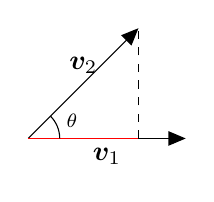
\begin{tikzpicture}
  \coordinate (v1) at (0,0);
  \coordinate (v2) at (2,0);
  \coordinate (v3) at (1.4,1.4);
  \coordinate (v4) at (1.4,0);
  % add coordinate at the extension of the line from v1 to v2
  \coordinate (v2-2) at ($(v1)!1.2!(v2)$); 

  \draw[->] (v1) -- node[below] {$\bm{v}_{1}$} (v2);
  \draw[->] (v1) -- node[above] {$\bm{v}_{2}$} (v3);
  \draw[red,-] (v1) -- node[below] {} (v4);
  \draw[dashed] (v4) -- node[below] {} (v3);

  % draw line and angle
  \draw 
     pic [draw,angle radius=4mm,angle eccentricity=1.5, "$\theta$" font=\scriptsize] {angle=v2--v1--v3};

\end{tikzpicture}

%    \caption{The shadow in red is equal to $cos(\theta) = \bm{v}_{1}^{T}\bm{v}_{2}$ ($\|\bm{v}_{1}\|_{2}= \|\bm{v}_{2}\|_{2} = 1$). The equality \ref{principal_angles_formula} is a generalization of this formula for multiple vectors.
%    \label{f:angles_between_subspaces}
%    }
%\end{figure}

\subsection{The Cosine Sine decomposition}
The Cosine Sine (CS) decomposition is useful for the study of the relative position of two subspaces. It generalizes the notion of cosine, sine and tangent to subspaces. The tangent of principal angles between subspaces were first mentioned in \citealp{ZhKn13}.
\begin{proposition}[\citealp{GoVa96}]
Let $q,d \in \mathbb{N}$ and $\bm{Q} =
\left[
\begin{array}{c}
\bm{Q}_{1}  \\
\hline
\bm{Q}_{2}
\end{array}
\right]
$ be a $d\times q$ orthogonal matrix, where $\bm{Q}_{1} \in \mathbb{R}^{q \times q}$ and $\bm{Q}_{2} \in \mathbb{R}^{(d-q)\times q}$. Assume that $\bm{Q}_{1}$ is non singular, then there exist orthogonal matrices $\bm{Y}\in\mathbb{R}^{d \times q}$ and
\begin{equation}
 \bm{W} =
\left[
\begin{array}{c|c}
\bm{W}_{1} & \bm{0} \\
\hline
\bm{0} & \bm{W}_{2}
\end{array}
\right]~\in~\mathbb{R}^{d \times d},
\end{equation}
%and $\bm{Y}~\in~\mathbb{R}^{d \times q}$,
and a matrix
\begin{equation}
\bm{\Sigma}~=~\left[
\begin{array}{c}
\Cosmatrix \\
\hline
\Sinmatrix \\
\hline
\bm{0}_{q',q}
\end{array}
\right] \in \mathbb{R}^{d \times q},
\end{equation}
where $q' = \max(0,d-2q)$, such that
\begin{equation}
    \bm{Q} = \bm{W}\bm{\Sigma}\bm{Y}^{T},
\end{equation}
where $\bm{W}_{1} \in \mathbb{R}^{q \times q}$ and $\bm{W}_{2} \in \mathbb{R}^{d-q \times d-q}$, and $\Cosmatrix, \Sinmatrix \in \mathbb{R}^{q\times q}$ are diagonal matrices satisfying the identity $\Cosmatrix^{2} + \Sinmatrix^{2} = \mathbb{I}_{q}$.
In particular, each block $\bm{Q}_{i}$ factorizes as
\begin{equation}
\begin{split}
    \bm{Q}_{1} = & \bm{W}_{1}\Cosmatrix\bm{Y}^{T} \\
    \bm{Q}_{2} = & \bm{W}_{2}\left[
\begin{array}{c}
\Sinmatrix \\
\hline
\bm{0}_{q',q}
\end{array}
\right]\bm{Y}^{T} .\\
\end{split}
\end{equation}

\label{CSD_proposition}
\end{proposition}
The CS decomposition is defined for every orthogonal matrix. An important case is when $\bm{Q}$ is the product of an orthogonal matrix $\bm{V} \in \mathbb{R}^{d \times d}$ and a sampling matrix $\bm{S} \in \mathbb{R}^{d \times k}$, that is $\bm{Q} = \bm{V}^{\Tran}\bm{S}$.

\begin{corollary}\label{corollary:tangent_of_principal_angles}
Let $\bm{V} \in \mathbb{R}^{d \times d}$ be an orthogonal matrix and $\bm{S} \in \mathbb{R}^{d \times k}$ be a sampling matrix. Let
\begin{equation}
\bm{Q} = \bm{V}^{\Tran}\bm{S} = \left[
\begin{array}{c}
\bm{V}_{k}^{\Tran} \bm{S}\\
\hline
\bm{V}_{k^{\perp}}^{\Tran} \bm{S}\\
\end{array}
\right]
\end{equation}
be a $d \times k$ orthogonal matrix, with $\Det(\bm{V}_{k}^{\Tran} \bm{S})^{2} > 0$. Let further $\bm{Z}_{S} = \bm{V}_{k^{\perp}}^{\Tran} \bm{S}(\bm{V}_{k}^{\Tran}\bm{S})^{-1}$. Then
\begin{equation}\label{eq:trace_tan_relationship}
\Tr(\bm{Z}_{S}^{}\bm{Z}_{S}^{\Tran}) = \sum\limits_{i \in [k]} \tan^{2}(\theta_{i}(S)),
%\Tr(\bm{Z}_{S}\bm{Z}_{S}^{\Tran}) = \sum\limits_{i \in [k]} \tan(\theta_{i})^{2}
\end{equation}
where the $(\theta_{i}(S))_{i \in [k]}$ are the principal angles between $\Span(\bm{V}_{k})$ and $\Span(\bm{S})$.
% \begin{equation}
% \Det(\bm{V}_{k}^{\Tran} \bm{S})^{2}\Tr(\bm{Z}_{S}^{}\bm{Z}_{S}^{\Tran}) = \prod\limits_{j \in [k]} \cos^{2}(\theta_{j}) \sum\limits_{i \in [k]} \tan^{2}(\theta_{i}) = e_{k-1}(\Lambda(\bm{V}_{k}^{\Tran}\bm{S})^{2}) - e_{k}(\Lambda(\bm{V}_{k}^{\Tran}\bm{S})^{2})
% \end{equation}
\end{corollary}

\begin{proof}
%\ab{finish the proof}\\
Proposition~\ref{CSD_proposition} applied to the matrix $\bm{Q} = \bm{V}^{\Tran}\bm{S}$ with $\bm{Q}_{1} = \bm{V}_{k}^{\Tran}\bm{S}$ and $\bm{Q}_{2} = \bm{V}_{k^{\perp}}^{\Tran} \bm{S}$ yields
\begin{align}\label{eq:common_factorization_Q_1}
    \bm{Q}_{1} = & \bm{W}_{1}\Cosmatrix\bm{Y}^{T} \\ \label{eq:common_factorization_Q_2}
    \bm{Q}_{2} = & \bm{W}_{2}\left[
\begin{array}{c}
\Sinmatrix \\
\hline
\bm{0}_{q',q}
\end{array}
\right]\bm{Y}^{T}.
\end{align}
Thus, the diagonal matrix $\Cosmatrix$ contains the singular values of the matrix $\bm{V}_{k}^{\Tran}\bm{S}$, which are cosines of the principal angles $(\theta_{i}(S))_{i \in [k]}$ between $\Span(\bm{V}_{k})$ and $\Span(\bm{S})$, see Proposition~\ref{principal_angles_theorem_1}.
%
The identity $\Cosmatrix^{2} + \Sinmatrix^{2} = \mathbb{I}_{k}$ and the fact that $\theta_{i}(S) \in [0, \frac{\pi}{2} ]$ imply  that the (diagonal) elements of $\Sinmatrix$ are equal to the sines of the principal angles between $\Span(\bm{V}_{k})$ and $\Span(\bm{S})$. Let $\Tanmatrix = \Sinmatrix \Cosmatrix^{-1}\in \mathbb{R}^{k \times k}$ be the diagonal matrix containing the tangents of the principal angles $(\theta_{i}(S))_{i \in [k]}$ on its diagonal. Using \eqref{eq:common_factorization_Q_1} and \eqref{eq:common_factorization_Q_2}, it comes
\begin{align}
\bm{Z}_{S} &= \bm{V}_{k^{\perp}}^{\Tran} \bm{S}(\bm{V}_{k}^{\Tran}\bm{S})^{-1}
= \bm{W}_{2}\left[
\begin{array}{c}
\Sinmatrix \\
\hline
\bm{0}_{q',q}
\end{array}
\right] \bm{Y}^{\Tran}\bm{Y} \Cosmatrix^{-1} \bm{W}_{1}^{\Tran} \nonumber\\
& = \bm{W}_{2}\left[
\begin{array}{c}
\Sinmatrix \\
\hline
\bm{0}_{q',q}
\end{array}
\right] \Cosmatrix^{-1} \bm{W}_{1}^{\Tran}  = \bm{W}_{2}\left[
\begin{array}{c}
\Sinmatrix \Cosmatrix^{-1}\\
\hline
\bm{0}_{q',q}
\end{array}
\right] \bm{W}_{1}^{\Tran}.
\end{align}
Then,
\begin{equation}
\Tr(\bm{Z}_{S}^{}\bm{Z}_{S}^{\Tran}) = \Tr(\bm{W}_{2}\left[
\begin{array}{c|c}
\Tanmatrix^{2} & \bm{0}_{q,q'}\\
\hline
\bm{0}_{q',q} & \bm{0}_{q',q'}
\end{array}
\right] \bm{W}_{2}^{\Tran})=  \sum\limits_{i \in [k]} \tan^{2}(\theta_{i}(S)).
\end{equation}
% Now if $k \geq \frac{d}{2}$
% The non vanishing singular values of the matrix $\bm{Z}_{S} = \bm{V}_{d-k}^{\Tran} \bm{S}(\bm{V}_{k}^{\Tran}\bm{S})^{-1}$ are the elements of the diagonal of the matrix $\Sinmatrix^{} \Cosmatrix^{-1}$: the tangents of the diagonal elements of the matrix $\Cosmatrix = \Diag(\cos(\theta_{i})_{i \in [k]})$.
\end{proof}

% Note the difference between Corollary~\ref{corollary:tangent_of_principal_angles} and the results proven in \citealp{DrIp18} that relates low rank approximations and principal angles between subspaces. The low rank approximation error in \citealp{DrIp18} was bounded by the sinus of principal angles between subspaces in $\mathbb{R}^{N}$ while Corollary~\ref{corollary:tangent_of_principal_angles} will be used to bound low rank approximation by the tangent of principal angles between subspaces in $\mathbb{R}^{d}$.
\cite*{DrIp19} have also related principal angles to low rank approximations. We consider different subspaces, though, which crucially put forward the tangents of the principal angles.

%We consider $\mathcal{P} = Span(\bm{X})$ and $\mathcal{Q} = Span(\bm{Y})$
%and we note $\bm{C}$ a diagonal matrix containing the cosines of principal angles between $\mathcal{P}$ and $\mathcal{Q}$.\\

%the tangents of the principal angles between $\mathcal{P}$ and $\mathcal{Q}$.



% \begin{proof}
% We consider the orthogonal matrix
% \begin{equation}
%     \bm{Q} = \hat{\bm{X}}^{T}\hat{\bm{Y}}=
% \left[
% \begin{array}{c|c}
% \bm{X}^{T}\bm{Y} & \bm{X}^{T}\bm{Y}_{\perp} \\
% \hline
% \bm{X}_{\perp}^{T}\bm{Y} & \bm{X}_{\perp}^{T}\bm{Y}_{\perp}
% \end{array}
% \right]
% \end{equation}


% According to proposition \ref{CSD_proposition}, there
%  exists unitary matrices $\bm{W} =
% \left[
% \begin{array}{c|c}
% \bm{W}_{1} & \bm{0} \\
% \hline
% \bm{0} & \bm{W}_{2}
% \end{array}
% \right]
% $, $\bm{Z} =
% \left[
% \begin{array}{c|c}
% \bm{Z}_{1} & \bm{0} \\
% \hline
% \bm{0} & \bm{Z}_{2}
% \end{array}
% \right]
% $ and a block diagonal matrix $\bm{\Sigma} = \left[
% \begin{array}{c|c}
% \bm{\Sigma}_{11} & \bm{\Sigma}_{12} \\
% \hline
% \bm{\Sigma}_{21} & \bm{\Sigma}_{22}
% \end{array}
% \right]$ such that we have:
% \begin{equation}
%     \bm{Q} = \bm{W}\bm{\Sigma}\bm{Z}^{T}
% \end{equation}
% We obtain a matrix factorization for each block $\bm{Q}_{i,j}$:
% \begin{align*}
%     \bm{Q}_{11} = & \bm{W}_{1}\bm{\Sigma}_{11}\bm{Z}_{1}^{T} \\
%     \bm{Q}_{12} = & \bm{W}_{1}\bm{\Sigma}_{12}\bm{Z}_{2}^{T} \\
%     \bm{Q}_{21} = & \bm{W}_{2}\bm{\Sigma}_{21}\bm{Z}_{1}^{T} \\
%     \bm{Q}_{22} = & \bm{W}_{2}\bm{\Sigma}_{22}\bm{Z}_{2}^{T} \\
% \end{align*}
% Such that there exist an integer $t$ and two diagonal matrices $\bm{C}, \bm{S} \in \mathbb{R}^{(l-t)\times(l-t)}$ with $\bm{C}^{2} + \bm{S}^{2} = \bm{I}_{l-t}$
% \begin{equation}
%     \bm{\Sigma}_{11} =
% \left[
% \begin{array}{c|c}
% \bm{I}_{t} & \bm{0} \\
% \hline
% \bm{0} & \bm{C}
% \end{array}
% \right], \bm{\Sigma}_{12} =
% \left[
% \begin{array}{c|c}
% \bm{0}_{t} & \bm{0} \\
% \hline
% \bm{0} & \bm{S}
% \end{array}
% \right], \bm{\Sigma}_{21} =
% \left[
% \begin{array}{c|c}
% \bm{S} & \bm{0} \\
% \hline
% \bm{0} & \bm{0}_{t}
% \end{array}
% \right],
% \bm{\Sigma}_{22} =
% \left[
% \begin{array}{c|c}
% -\bm{C} & \bm{0} \\
% \hline
% \bm{0} & \bm{I}_{t}
% \end{array}
% \right]
% \end{equation}
% We have
% \begin{equation}
%     \bm{T} = \bm{Q}_{21}\bm{Q}_{11}^{+} = \bm{W}_{2}\bm{\Sigma}_{21}\bm{\Sigma}_{11}^{+}\bm{W}_{1}
% \end{equation}
% \todo{finish this}
% \end{proof}



\section{Proofs}
\label{app:proofs}


%\subsection{proofs}\label{proofs}
\subsection{Technical lemmas}
We start with two useful lemmas borrowed from the literature.
\begin{lemma}[Lemma 3.1, \citealp{BoDrMI11}]\label{refined_analysis_of_approximation_bound}
Let $S \subset [d]$, then
%, and let $\bm{S} \in \{0,1\}^{d \times k}$ be the corresponding sampling matrix: $\bm{S}$ is defined by $\forall \bm{M} \in \mathbb{R}^{N\times d}, \bm{M}\bm{S} = \bm{M}_{.,S}$.

\begin{equation}
\| \bm{X} - \Pi_{S,k}^{\nu} \bm{X} \|_{\nu}^{2}  \leq  \| \bm{E}(\bm{I}-\bm{P}_{S})\|_{\nu}^{2}, \quad \nu \in \{2,\Fr\},
\end{equation}
where   $\bm{E} = \bm{X} - \Pi_{k}\bm{X}$ and $\bm{P}_{S} = \bm{S}(\bm{V}_{k}^{\Tran}\bm{S})^{-1}\bm{V}_{k}^{\Tran}$.
%In particular, we have for the Frobenius norm:
%\begin{equation}
%\| \bm{X} - \Pi_{S}\bm{X} \|_{\Fr}^{2}  \leq  \| \bm{E}\|_{\Fr}^{2} + \Tr(\bm{E}\bm{E}^{\Tran}\bm{P}\bm{P}^{\Tran})
%\end{equation}
Furthermore,
\begin{equation}
\| \bm{X} - \Pi_{S,k}^{\nu} \bm{X} \|_{\nu}^{2} \leq  \frac{1}{\sigma_{k}^{2}(\bm{V}_{S,[k]})} \| \bm{X} - \Pi_{k}\bm{X}\|_{\nu}^{2} , \quad \nu \in \{2,\Fr\}.
\end{equation}
\end{lemma}
The following lemma was first proven by \citealp{DRVW06}, and later rephrased in \cite{DeRa10}.
\begin{lemma}[Lemma 11, \citealp{DeRa10}]\label{minors_symmetric_polynomials_lemma}
Let $\bm{V} \in \mathbb{R}^{k \times d}$, $r = \rank(\bm{V})$ and $\ell \in [1:r]$. Then
\begin{equation}
\sum\limits_{S \subset [d], |S| = \ell} e_{\ell}(\Sigma(\bm{V}_{:,S})^{2}) = e_{\ell}(\Sigma(\bm{V})^{2})
\end{equation}
where $e_{\ell}$ is the $\ell$-th elementary symmetric polynomial on $r$ variables, see Section~\ref{s:notation}.
\end{lemma}
%\begin{example}
%Let $\bm{V} \in \bm{R}^{r \times n}$ a rectangular matrix with orthonormal rows. The singular values of $\bm{V}$ are $\bm{\Sigma} = (1,...,1,0,...,0 )$ ($\bm{\Sigma}$ contains $r$ ones and $n-r$ zero). Using the Lemma~\ref{minors_symmetric_polynomials_lemma} we get the following identities:
%\begin{itemize}
%    \item $\sum\limits_{S \subset [n], |S| = r} \Det(\bm{V}_{.,S})^{2} = 1$
%    \item $\sum\limits_{S \subset [n], |S| = r-1} \Det(\bm{V}_{.,S})^{2} = r$
%\end{itemize}
%\end{example}
Elementary symmetric polynomials play an important role in the proof of Proposition~\ref{prop:p_eff_proposition}, in particular their interplay with the Schur order; see Appendix \ref{app:majorization} for definitions.

\begin{lemma}\label{symmetric_schur_convex_lemma}
Let $\phi, \psi:\mathbb{R}_{+}^{*^{k}} \rightarrow \mathbb{R}_{+}^{*}$ be defined by
\begin{equation}
\phi :  \bm{\sigma} \mapsto \frac{\displaystyle e_{k-1}(\bm{\sigma})}{\displaystyle e_{k}(\bm{\sigma})}
\end{equation}
and
\begin{equation}
\psi :  \bm{\sigma} \mapsto \displaystyle e_{k}(\bm{\sigma}).
\end{equation}
% $\psi : \bm{\sigma} \mapsto e_{k}(\bm{\sigma})$
Then both functions are symmetric, $\phi$ is Schur-convex, and $\psi$ is Schur-concave.
\end{lemma}
\begin{proof}[of Lemma~\ref{symmetric_schur_convex_lemma}]
Let $i,j \in [k], i \neq j$. Let $\sigma_{i},\sigma_{j} \in \mathbb{R}_{+}^{*}$, it holds
\begin{align*}
    (\sigma_{i} - \sigma_{j})(\partial_{i}\phi(\bm{\sigma})-\partial_{j}\phi(\bm{\sigma})) & =  (\sigma_{i} - \sigma_{j})(-\frac{1}{\sigma_{i}^{2}} +\frac{1}{\sigma_{j}^{2}}) \\
    & = \frac{(\sigma_{i}-\sigma_{j})^{2}(\sigma_{i} +\sigma_{j})}{\sigma_{i}^{2}\sigma_{j}^{2}} \geq 0,%\\
%    & \geq 0,
\end{align*}
so that $\phi$ is Schur-convex by Proposition~\ref{schur_order_partial_property}. Similarly,
\begin{align*}
    (\sigma_{i} - \sigma_{j})(\partial_{i}\psi(\bm{\sigma})-\partial_{j}\psi(\bm{\sigma})) & =  (\sigma_{i} - \sigma_{j})(\prod_{\ell \neq i}\sigma_{\ell} - \prod_{\ell \neq j}\sigma_{\ell}) \\
    & = -(\sigma_{i}-\sigma_{j})^{2}\prod_{\ell \neq i,j}\sigma_{\ell} \geq 0, %\\
%    & \leq 0.
\end{align*}
so that $\psi$ is Schur-concave by Proposition~\ref{schur_order_partial_property}.
\end{proof}

Elementary symmetric polynomials also interact nicely with ``marginalizing" sums.
%%%% LEMMA 32
\begin{lemma}\label{sum_k_1_symmetric_poly_det_lemma}
Let $\bm{V}$ be a real $k \times d$ matrix and let $ r = \rank(\bm{V})$. Denote by $p$ the number of non zero columns of $\bm{V}$. Then for all $k\leq r+1$,
\begin{equation}
    \sum\limits_{\substack{S \subset [d], |S| = k\\\Vol_{k}(\bm{V}_{:,S})^{2} >0}} \quad \sum\limits_{\substack{T \subset S \\ |T| = k-1}} e_{k-1}(\Sigma(\bm{V}_{:,T})^{2}) \leq (p-k+1)e_{k-1}(\Sigma(\bm{V})^{2}).
\end{equation}
A fortiori,
\begin{equation}
    \sum\limits_{\substack{S \subset [d], |S| = k\\\Vol_{k}(\bm{V}_{:,S})^{2} >0}} \quad \sum\limits_{\substack{T \subset S \\ |T| = k-1}} e_{k-1}(\Sigma(\bm{V}_{:,T})^{2}) \leq (d-k+1)e_{k-1}(\Sigma(\bm{V})^{2}).
\end{equation}
\end{lemma}

%%%%%%%%%%%%%%%%%%%
\begin{proof}[of Lemma~\ref{sum_k_1_symmetric_poly_det_lemma}]
%Recall that $\sigma_{1}(\bm{V}), \dots ,\sigma_{r}(\bm{V})$ are the non zeros singular values of $\bm{V}$.
For $T \subset [d], \: |T| = k-1$,
\begin{align*}
    \Omega_{1}(T) &= \left\{ S \subset[d]:\, |S| = k, T \subset S,\ \forall i \in S ,\ \bm{V}_{:,i} \neq \bm{0} \right\}\\
    \Omega_{2}(T) &= \left\{ S \subset[d] :\, |S| = k, T \subset S, \Vol_{k}(\bm{V}_{:,S})^{2} >0   \right\}.
\end{align*}
Note that $\Omega_{2}(T) \subset \Omega_{1}(T)$ so that
\begin{align*}
        \sum\limits_{\substack{S \subset [d], |S| = k\\\Vol_{k}(\bm{V}_{:,S})^{2} >0}} \quad \sum\limits_{\substack{T \subset S\\ |T| = k-1}} e_{k-1}(\Sigma(\bm{V}_{:,T})^{2})
        & = \sum\limits_{\substack{T \subset [d]\\ |T| = k-1}} \quad \sum\limits_{S \in \Omega_{2}(T)} e_{k-1}(\Sigma(\bm{V}_{:,T})^{2}) \\
        & \leq \sum\limits_{\substack{T \subset [d]\\ |T| = k-1}} \quad \sum\limits_{S \in \Omega_{1}(T)} e_{k-1}(\Sigma(\bm{V}_{:,T})^{2}).
\end{align*}
The set $\Omega_{1}(T)$ has at most $(p-k+1)$ elements so that
\begin{equation}
\sum\limits_{\substack{T \subset [d]\\ |T| = k-1}} \quad \sum\limits_{S \in \Omega_{1}(T)} e_{k-1}(\Sigma(\bm{V}_{:,T})^{2}) \leq (p-k+1)\sum\limits_{\substack{T \subset [d]\\ |T| = k-1}}  e_{k-1}(\Sigma(\bm{V}_{:,T})^{2}).
\end{equation}
Lemma~\ref{minors_symmetric_polynomials_lemma} for $\ell=k-1$ further yields
\begin{equation}
(p-k+1)\sum\limits_{\substack{T \subset [d]\\ |T| = k-1}}  e_{k-1}(\Sigma(\bm{V}_{:,T})^{2}) \leq (p-k+1)\,e_{k-1}(\Sigma(\bm{V})^{2}).
\end{equation}
\end{proof}

%%%%%%%%%%%%%%%%%%%
\subsection{Proof of Proposition~\ref{projection_dpp_theorem}}
%\begin{proof}[of Theorem~\ref{projection_dpp_theorem}]
First, Lemma~\ref{refined_analysis_of_approximation_bound} yields
	\begin{align}
	\sum\limits_{S \subset [d], |S| = k} \Det(\bm{V}_{S,[k]})^{2}\| \bm{X} - \Pi_{S}^{\nu}\bm{X} \|_{\nu}^{2} & \leq  \sum\limits_{S 	\subset [d], |S| = k} \frac{1}{\sigma_{k}^{2}(\bm{V}_{S,[k]})}\Det(\bm{V}_{S,[k]})^{2} \: \|\bm{X} - \Pi_{k}\bm{X}\|_{\nu}^{2}  \nonumber\\
 	& =  \|\bm{X} - \Pi_{k}\bm{X}\|_{\nu}^{2} \sum\limits_{S \subset [d], |S| = k} \prod_{\ell =1}^{k-1}\sigma_{\ell}^{2}(\bm{V}_{S,[k]}),
 % & \leq \sum\limits_{S \subset [d], |S| = k} e_{k-1}((\sigma_{\ell}^{2}(\bm{V}_{S,[k]})_{1\leq \ell \leq k})) \: \|\bm{X} - \Pi_{k}\bm{X}\|_{\nu}^{2} \\
 % & \leq \sum\limits_{S \subset [d], |S| = k} \sum\limits_{T \subset S, |T| = k-1} \Vol_{k-1}(\bm{V}_{T,[k]})^{2} \: \|\bm{X} - \Pi_{k}\bm{X}\|_{\nu}^{2}.
 \label{eq:begin_proof_theo16}
\end{align}
where the last equality follows from
\begin{equation}
	\Det(\bm{V}_{S,[k]})^{2} = \prod_{\ell =1}^{k}\sigma_{\ell}^{2}(\bm{V}_{S,[k]}).
\end{equation}
%%
By definition of the polynomial $e_{k-1}$, it further holds
\begin{equation}
	\prod_{\ell =1}^{k-1}\sigma_{\ell}^{2}(\bm{V}_{S,[k]}) \leq e_{k-1}(\Sigma(\bm{V}_{S,[k]})^{2}),
\end{equation}
so that \eqref{eq:begin_proof_theo16} leads to
\begin{align}
\sum\limits_{S \subset [d], |S| = k} \Det(\bm{V}_{S,[k]})^{2}\| \bm{X} - \Pi_{S}^{\nu}\bm{X} \|_{\nu}^{2} & \leq  \|\bm{X} - \Pi_{k}\bm{X}\|_{\nu}^{2} \sum\limits_{S \subset [d], |S| = k} e_{k-1}(\Sigma(\bm{V}_{S,[k]})^{2}).
% & \leq \sum\limits_{S \subset [d], |S| = k} e_{k-1}((\sigma_{\ell}^{2}(\bm{V}_{S,[k]})_{1\leq \ell \leq k})) \: \|\bm{X} - \Pi_{k}\bm{X}\|_{\nu}^{2} \\
% & \leq \sum\limits_{S \subset [d], |S| = k} \sum\limits_{T \subset S, |T| = k-1} \Vol_{k-1}(\bm{V}_{T,[k]})^{2} \: \|\bm{X} - \Pi_{k}\bm{X}\|_{\nu}^{2}.
\label{eq:middle_proof_theo16}
\end{align}

Now, Lemma~\ref{minors_symmetric_polynomials_lemma} applied to the matrix $\bm{V}^{\Tran}_{S,[k]}$ gives
\begin{equation}
	e_{k-1}(\Sigma(\bm{V}_{S,[k]})^{2}) = \sum\limits_{T \subset S, |T| = k-1} e_{k-1}(\Sigma(\bm{V}_{T,[k]})^{2}),
\end{equation}
Therefore, Lemma~\ref{sum_k_1_symmetric_poly_det_lemma} yields
\begin{equation}
\label{eq:const_dpluskmoins1}
\begin{split}
%% \sum\limits_{S \subset [d], |S| = k} \Det(\bm{V}_{S,[k]})^{2}\| \bm{X} - \Pi_{S}\bm{X} \|_{\nu}^{2} & \leq  \sum\limits_{S \subset [d], |S| = k} \frac{1}{\sigma_{k}^{2}(\bm{V}_{S,[k]})}\Det(\bm{V}_{S,[k]})^{2} \: \|\bm{X} - \Pi_{k}\bm{X}\|_{\nu}^{2}  \\
%%  & \leq
\sum\limits_{S \subset [d], |S| = k} e_{k-1}(\Sigma(\bm{V}_{S,[k]})^{2})
  & \leq (d-k+1)\sum\limits_{T \subset [d], |T| = k-1} e_{k-1}(\Sigma(\bm{V}_{T,[k]})^{2}).\\
%\sum\limits_{S \subset [d], |S| = k} \prod_{\ell =1}^{k-1}\sigma_{\ell}^{2}(\bm{V}_{S,[k]}) \: \|\bm{X} - \Pi_{k}\bm{X}\|_{\nu}^{2}
%  & \leq \sum\limits_{S \subset [d], |S| = k} e_{k-1}(\Sigma(\bm{V}_{S,[k]})^{2}) \: \|\bm{X} - \Pi_{k}\bm{X}\|_{\nu}^{2} \\
%  & \leq \sum\limits_{S \subset [d], |S| = k} \sum\limits_{T \subset S, |T| = k-1} e_{k-1}(\Sigma(\bm{V}_{T,[k]})^{2}) \: \|\bm{X} - \Pi_{k}\bm{X}\|_{\nu}^{2}\\
%  & \leq (d-k+1)\sum\limits_{T \subset [d], |T| = k-1} e_{k-1}(\Sigma(\bm{V}_{T,[k]})^{2}) \: \|\bm{X} - \Pi_{k}\bm{X}\|_{\nu}^{2}.\\
\end{split}
\end{equation}
Using Lemma~\ref{minors_symmetric_polynomials_lemma} and the fact that $\bm{V}_{k}$ is orthogonal, we finally write
\begin{equation}
\label{eq:const_k}
\sum\limits_{T \subset [d], |T| = k-1} e_{k-1}(\Sigma(\bm{V}_{T,[k]})^{2}) = e_{k-1}(\Sigma(\bm{V}_{k})^{2}) = k.
\end{equation}
Plugging \eqref{eq:const_k} into \eqref{eq:const_dpluskmoins1}, and then into (\ref{eq:middle_proof_theo16}) concludes the proof of Proposition~\ref{projection_dpp_theorem}.
%\end{proof}

%%%%%%%%%%%%%%%%%%   Proof of proposition 17    %%%%%%%%
\subsection{Proof of Proposition \ref{hypo_one_two_proposition}}
\label{s:proofOfExactSparsitySetting}
%\begin{proof}[]
We first prove the Frobenius norm bound, which requires more work. The spectral bound is easier and uses a subset of the arguments for the Frobenius norm.

\subsubsection{Frobenius norm bound}
\label{s:frobNormThm19}
%\paragraph{}
Recall that $\bm{E} = \bm{X} - \Pi_{k}\bm{X}$.
We start with Lemma~\ref{refined_analysis_of_approximation_bound}:
\begin{equation}
\label{eq:begin_proof_prop17}
	\begin{split}
		\| \bm{X} - \Pi_{S}^{\Fr}\bm{X} \|_{\Fr}^{2}  & \leq  \| \bm{E}(\bm{I}-\bm{P}_{S})\|_{\Fr}^{2}\\
		& = \| \bm{E}\|_{\Fr}^{2} + \Tr(\bm{E}^{\Tran}\bm{E}\bm{P}_{S}\bm{P}_{S}^{\Tran}) - 2\Tr(\bm{P}_{S}^{\Tran}		\bm{E}^{\Tran}\bm{E}).
	\end{split}
\end{equation}
Since $\bm{E}^{\Tran}\bm{E} = \bm{V}_{k^{\perp}}^{\phantom{\Tran}}\bm{\Sigma}_{k^{\perp}}^{2}\bm{V}_{k^{\perp}}^{\Tran}$ and $\bm{P}_{S} = \bm{S}(\bm{V}_{k}^{\Tran}\bm{S})^{-1}\bm{V}_{k}^{\Tran}$,
\begin{equation}
        \begin{split}
        		\Tr(\bm{P}_{S}^{\Tran}\bm{E}^{\Tran}\bm{E})  & =  \Tr \bigg(\bm{V}_{k}^{\phantom{\Tran}}((\bm{V}_{k}^{\Tran}		\bm{S})^{\Tran})^{-1}\bm{S}^{\Tran}\bm{V}_{k^{\perp}}^{\phantom{\Tran}}\bm{\Sigma}_{k^{\perp}}^{\phantom{\Tran}}\bm{V}		_{k^{\perp}}^{\Tran} \bigg)  \\
        		& = \Tr \bigg( \bm{V}_{k^{\perp}}^{\Tran}\bm{V}_{k}^{\phantom{\Tran}}((\bm{V}_{k}^{\Tran}\bm{S})^{\Tran})^{-1}\bm{S}		^{\Tran}\bm{V}_{k^{\perp}}^{\phantom{\Tran}}\bm{\Sigma}_{k^{\perp}}^{\phantom{\Tran}} \bigg)  \\
      		  & = 0,
        \end{split}
\end{equation}
where the last equality follows from $\bm{V}_{k^{\perp}}^{\Tran}\bm{V}_{k} = \bm{0}$.
Therefore, (\ref{eq:begin_proof_prop17}) becomes
\begin{equation}
	\| \bm{X} - \Pi_{S}^{\Fr}\bm{X} \|_{\Fr}^{2}  \leq \| \bm{E}\|_{\Fr}^{2} + \Tr(\bm{E}^{\Tran}\bm{E}\bm{P}^{\phantom{\Tran}}	_{S}\bm{P}^{\Tran}_{S}).
\end{equation}
% \begin{equation}
% \| \bm{X} - \Pi_{S}\bm{X} \|_{\Fr}^{2}  \leq  \| \bm{E}\|_{\Fr}^{2} + \Tr(\bm{E}\bm{E}^{\Tran}\bm{P}\bm{P}^{\Tran})
% \end{equation}
Taking expectations,
\begin{equation}
  \label{eq:inequality_approximation_error_by_EEPP}
		\EX_{\DPP} \| \bm{X} - \Pi_{S}^{\Fr}\bm{X} \|_{\Fr}^{2} \leq \|\bm{E}\|_{\Fr}^{2} + \sum_{S \subset [d], |S| = k}	\Det(\bm{V}_{S,[k]})^{2} \Tr(\bm{E}^{\Tran}\bm{E}\bm{P}^{\phantom{\Tran}}_{S}\bm{P}^{\Tran}_{S}).
\end{equation}
Proposition~\ref{principal_angles_theorem_1} expresses $\Det(\bm{V}_{S,[k]})^{2}$ as a function of the principal angles $(\theta_i(S))$ between $\Span(\bm{V}_k)$ and $\Span(\bm{S})$, namely
\begin{equation}\label{eq:det_cos_identity}
	\Det(\bm{V}_{S,[k]})^{2} = \prod\limits_{i \in [k]} \cos^{2}(\theta_{i}(S)).
\end{equation}
 The remainder of the proof is in two steps. First, we bound the second factor in the sum in the right-hand side of \eqref{eq:inequality_approximation_error_by_EEPP} with a similar geometric expression. This allows trigonometric manipulations. Second, we work our way back to elementary symmetric polynomials of spectra, and we conclude after some simple algebra.

First, for $S \subset [d], |S| =k$, let
$$
\bm{Z}_{S} = \bm{V}_{k^{\perp}}^{\Tran} \bm{S}(\bm{V}_{k}^{\Tran}\bm{S})^{-1} = \bm{V}_{k^{\perp}}^{\Tran} \bm{P}_{S}^{\phantom{\Tran}} \bm{V}_{k}.
$$
It allows us to write
\begin{equation}
	\Tr(\bm{E}^{\Tran}\bm{E}\bm{P}^{\phantom{\Tran}}_{S}\bm{P}^{\Tran}_{S})= \Tr(\bm{V}_{k^{\perp}}\bm{\Sigma}_{k^{\perp}}		^{2}\bm{V}_{k^{\perp}}^{\Tran}\bm{P}^{\phantom{\Tran}}_{S}\bm{P}^{\Tran}_{S}) = \Tr(\bm{\Sigma}_{k^{\perp}}^{2}\bm{Z}_{S}^{\phantom{\Tran}}\bm{V}_{k}^{\phantom{\Tran}}\bm{V}_{k}^{\Tran}\bm{Z}_{S}^{\Tran}).
\end{equation}
However, for real symmetric matrices $\bm{A}$ and $\bm{B}$ with the same size, a simple diagonalization argument yields
\begin{equation}
	\Tr(\bm{A}\bm{B}) \leq \|\bm{A}\|_{2}\Tr(\bm{B}),
\end{equation}
so that
% \begin{equation}\label{eq:majoration_by_sigma_k_1}
% 	\Tr(\bm{E}^{\Tran}\bm{E}\bm{P}^{\phantom{\Tran}}_{S}\bm{P}^{\Tran}_{S}) = \Tr(\bm{\Sigma}_{d-k}^{2}\bm{Z}_{S}^{\phantom{\Tran}}\bm{V}_{k}^{\phantom{\Tran}}\bm{V}_{k}^{\Tran}\bm{Z}_{S}^{\Tran}) = \Tr(\bm{Z}_{S}^{\Tran}\bm{\Sigma}_{d-k}^{2}\bm{Z}_{S}^{\phantom{\Tran}}\bm{V}_{k}^{\phantom{\Tran}}\bm{V}_{k}^{\Tran}) \leq \Tr(\bm{Z}_{S}^{\Tran}\bm{\Sigma}_{d-k}^{2}\bm{Z}_{S}^{\phantom{\Tran}}) \|\bm{V}_{k}^{\phantom{\Tran}}\bm{V}_{k}^{\Tran}\|_{2} \leq \bm{\sigma}_{k+1}^{2} \Tr(\bm{Z}_{S}^{\phantom{\Tran}}\bm{Z}_{S}^{\Tran}).
% \end{equation}
\begin{align}\label{eq:majoration_by_sigma_k_1}
\Tr(\bm{E}^{\Tran}\bm{E}\bm{P}^{\phantom{\Tran}}_{S}\bm{P}^{\Tran}_{S}) & = \Tr(\bm{\Sigma}_{k^{\perp}}^{2}\bm{Z}_{S}^{\phantom{\Tran}}\bm{V}_{k}^{\phantom{\Tran}}\bm{V}_{k}^{\Tran}\bm{Z}_{S}^{\Tran}) \nonumber\\
& = \Tr(\bm{Z}_{S}^{\Tran}\bm{\Sigma}_{k^{\perp}}^{2}\bm{Z}_{S}^{\phantom{\Tran}}\bm{V}_{k}^{\phantom{\Tran}}\bm{V}_{k}^{\Tran}) \nonumber\\
& \leq \Tr(\bm{Z}_{S}^{\Tran}\bm{\Sigma}_{k^{\perp}}^{2}\bm{Z}_{S}^{\phantom{\Tran}}) \|\bm{V}_{k}^{\phantom{\Tran}}\bm{V}_{k}^{\Tran}\|_{2} \nonumber\\
& \leq \Tr(\bm{Z}_{S}^{\Tran}\bm{\Sigma}_{k^{\perp}}^{2}\bm{Z}_{S}^{\phantom{\Tran}}) \nonumber \\
& \leq \|\bm{\Sigma}_{k^{\perp}}^{2}\|_{2}\Tr(\bm{Z}_{S}^{\phantom{\Tran}}\bm{Z}_{S}^{\Tran}) \nonumber \\
& \leq \bm{\sigma}_{k+1}^{2} \Tr(\bm{Z}_{S}^{\phantom{\Tran}}\bm{Z}_{S}^{\Tran}).
\end{align}

In Appendix~\ref{app:principal_angles}, we characterize $\Tr(\bm{Z}_{S}^{\phantom{\Tran}}\bm{Z}_{S}^{\Tran})$ using principal angles, see \eqref{eq:trace_tan_relationship}. This reads
\begin{equation}\label{eq:trace_tan_identity}
 	\Tr( \bm{Z}_{S}^{\phantom{\Tran}}\bm{Z}_{S}^{\Tran}) = \sum_{j \in [k]}\tan^{2}(\theta_{j}(S)).
\end{equation}
Combining \eqref{eq:inequality_approximation_error_by_EEPP}, \eqref{eq:majoration_by_sigma_k_1}, \eqref{eq:det_cos_identity}, and \eqref{eq:trace_tan_identity}, we obtain the following intermediate bound
\begin{equation}\label{eq:sum_product_cos_tan}
 	\EX_{\DPP} \| \bm{X} - \Pi_{S}^{\Fr}\bm{X} \|_{\Fr}^{2} \leq \| \bm{E}\|_{\Fr}^{2} + \bm{\sigma}_{k+1}^{2} \sum_{S \subset 	[d], |S| = k} \,\left[\prod\limits_{i \in [k]} \cos^{2}(\theta_{i}(S))\right] \left[\sum_{j \in [k]}\tan^{2}(\theta_{j}(S))\right].
\end{equation}
Distributing the sum and using trigonometric identities, the general term of the sum in \eqref{eq:sum_product_cos_tan} becomes
\begin{align}
    	\left[\prod\limits_{i \in [k]} \cos^{2}(\theta_{i}(S))\right] \left[\sum_{j \in [k]}\tan^{2}(\theta_{j}(S))\right] & =  \sum_{i \in [k]}(1-\cos^{2}(\theta_{i}(S)))\prod_{j \in [k], j 	\neq i} \cos^{2}(\theta_{j}(S)) \nonumber \\
    	& = \sum_{i \in [k]}\prod_{j \in [k], j \neq i} \cos^{2}(\theta_{j}(S)) - \sum_{i \in [k]}\prod_{j \in [k]}\cos^{2}(\theta_{j}(S)).
	\label{eq:prod_cos_tan_ineq}
\end{align}
The $(\cos(\theta_{j}(S)))_{j \in [k]}$ are the singular values of the matrix $\bm{V}_{S,[k]}$ so that
\begin{equation}\label{eq:cos_k_1_symmetric_polynomial_identity}
	\sum_{i \in [k]}\prod_{j \in [k], j \neq i} \cos^{2}(\theta_{j}(S)) = e_{k-1}(\Sigma(\bm{V}_{S,[k]})^{2}),
\end{equation}
and
\begin{equation}\label{eq:cos_k_symmetric_polynomial_identity}
	\prod_{j \in [k]}\cos^{2}(\theta_{j}(S)) = e_{k}(\Sigma(\bm{V}_{S,[k]})^{2}).
\end{equation}
Back to \eqref{eq:prod_cos_tan_ineq}, one gets
\begin{align}
    \left[\prod\limits_{i \in [k]} \cos^{2}(\theta_{i}(S))\right] \left[\sum_{j \in [k]}\tan^{2}(\theta_{j}(S))\right]
    & = e_{k-1}(\Sigma(\bm{V}_{S,[k]})^{2}) - \sum_{i \in [k]} e_{k}(\Sigma(\bm{V}_{S,[k]})^{2}) \nonumber\\
    & = e_{k-1}(\Sigma(\bm{V}_{S,[k]})^{2}) -  k e_{k}(\Sigma(\bm{V}_{S,[k]})^{2}). \label{eq:sumcostan} %%% LABEL UTILE
\end{align}
Thus, plugging \eqref{eq:sumcostan} back into the intermediate bound \eqref{eq:sum_product_cos_tan}, it comes
\begin{align}\label{eq:bound_tan_in_expectation_under_sparsity}
    \EX_{\DPP} \| \bm{X} &- \Pi_{S}^{\Fr}\bm{X} \|_{\Fr}^{2}\nonumber\\
     % &\leq \| \bm{E}\|_{\Fr}^{2} + \bm{\sigma}_{k+1}^{2} \sum\limits_{S \subset [d], |S| = k} \left[\prod\limits_{i \in [k]} \cos^{2}(\theta_{i}(S))\right]\left[\sum_{j \in [k]}\tan^{2}(\theta_{j}(S))\right]\nonumber\\
      &\leq \| \bm{E}\|_{\Fr}^{2} + \bm{\sigma}_{k+1}^{2} \left[\sum\limits_{\substack{S \subset [d]\\ |S| = k}} e_{k-1}(\Sigma(\bm{V}_{S,[k]})^{2}) -  k \sum_{\substack{S \subset [d]\\ |S| = k}}e_{k}(\Sigma(\bm{V}_{S,[k]})^{2})\right]\nonumber.\\
\end{align}
Using Lemma~\ref{minors_symmetric_polynomials_lemma} twice, it comes
\begin{align}
  \EX_{\DPP} \| \bm{X} &- \Pi_{S}^{\Fr}\bm{X} \|_{\Fr}^{2} \nonumber\\
  &\leq \| \bm{E}\|_{\Fr}^{2} + \bm{\sigma}_{k+1}^{2} \left[\sum_{\substack{S \subset [d]\\ |S| = k}} \,\sum_{\substack{T \subset S\\ |T| = k-1}} e_{k-1}(\Sigma(\bm{V}_{T,[k]})^{2}) -  ke_{k}(\Sigma(\bm{V}_{:,[k]})^{2})\right]
  \label{e:doubleSumTrick}.
\end{align}

Lemmas~\ref{sum_k_1_symmetric_poly_det_lemma} and the identities $e_{k-1}(\Sigma(\bm{V}_{:,[k]})^{2}) = k$ and $e_{k}(\Sigma(\bm{V}_{:,[k]})^{2}) = 1$ allow us to conclude
\begin{align}
  \EX_{\DPP} \| \bm{X} - \Pi_{S}^{\Fr}\bm{X} \|_{\Fr}^{2} &\leq \| \bm{E}\|_{\Fr}^{2} + \bm{\sigma}_{k+1}^{2} \left[ (p-k+1)e_{k-1}(\Sigma(\bm{V}_{:,[k]})^{2}) -  k \right]\\
  &=\| \bm{E}\|_{\Fr}^{2} + \bm{\sigma}_{k+1}^{2} (p-k)k.
\end{align}
By definition of $\beta$ \eqref{e:defbeta}, we have proven \eqref{eq:frobenius_bound_dpp}, i.e.,
\begin{align*}
    \EX_{\DPP} \| \bm{X} - \Pi_{S}^{\Fr}\bm{X} \|_{\Fr}^{2}
  & \leq \| \bm{E}\|_{\Fr}^{2} \left(1 + \beta \frac{p-k}{d-k}k \right).
\end{align*}
%\end{subsubsection}
%\paragraph{Spectral norm bound}



%%%%%%%%%%%% Spectral norm bound
\subsubsection{Spectral norm bound}
The bound in spectral norm is easier to derive.
We start with Lemma~\ref{refined_analysis_of_approximation_bound}:
\begin{equation}
\label{eq:begin_proof_prop17_spectral}
    \begin{split}
        \| \bm{X} - \Pi_{S}^{2}\bm{X} \|_{2}^{2}  & \leq  \| \bm{E}(\bm{I}-\bm{P}_{S})\|_{2}^{2}\\
        & \leq \| \bm{E}\|_{2}^{2} +  \| \bm{E}\bm{P}_{S}\|_{2}^{2}\\
        & \leq \| \bm{E}\|_{2}^{2} + \|\bm{E}\|_{2}^{2}\|\bm{V}_{k^{\perp}}^{\Tran}\bm{S}(\bm{V}_{k}^{\Tran}\bm{S})^{-1}\bm{V}_{k}^{\Tran}\|_{2}^{2}\\
        & \leq \| \bm{E}\|_{2}^{2}(1 + \|\bm{Z}_{S}\|_{2}^{2}),
    \end{split}
\end{equation}
where the notation is the same as in Section~\ref{s:frobNormThm19}.
Now
\begin{equation}\label{eq:bound_spectral_frob_proof_prop17_spectral}
                \|\bm{Z}_{S}\|_{2}^{2}  \leq  \|\bm{Z}_{S}\|_{\Fr}^{2}
                = \sum\limits_{i \in [k]} \tan^{2}(\theta_{i}(S)),
\end{equation}
thus by \eqref{eq:begin_proof_prop17_spectral}, \eqref{eq:bound_spectral_frob_proof_prop17_spectral} and \eqref{eq:det_cos_identity}
\begin{align}
    \EX_{\DPP} \| \bm{X} - \Pi_{S}^{2}\bm{X} \|_{2}^{2} &= \sum_{S \subset [d], |S| = k}\Det(\bm{V}_{S,[k]})^{2}\| \bm{X} - \Pi_{S}\bm{X} \|_{2}^{2}\\
    & \leq \| \bm{E}\|_{2}^{2} \left(1 + \sum_{\substack{S \subset [d], |S| = k\\   \Det(\bm{V}_{S,[k]})^{2}>0}} \prod\limits_{i =1}^{k} \cos^{2}(\theta_{i}(S)) \sum\limits_{i \in [k]} \tan^{2}(\theta_{i}(S)) \right).
\end{align}
By \eqref{eq:prod_cos_tan_ineq}, it comes
% \begin{equation}
%   \sum_{S \subset [d], |S| = k}\Det(\bm{V}_{S,[k]})^{2}\| \bm{X} - \Pi_{S}\bm{X} \|_{2}^{2} \leq \sum_{S \subset [d], |S| = k} \prod\limits_{l \in [k], l < k} \sigma_{l}^{2}(\bm{V}_{S,[k]})  \| \bm{E}\|_{2}^{2} \leq \sum_{S \subset [d], |S| = k} e_{k-1}(\Sigma(\bm{V}_{S,[k]})^{2})  \| \bm{E}\|_{2}^{2}
% \end{equation}
% and we finally get
\begin{align*}
    \EX_{\DPP} \| \bm{X} - \Pi_{S}^{2}\bm{X} \|_{2}^{2} & \leq  \| \bm{E}\|_{2}^{2} \left(1+\sum_{\substack{S \subset [d], |S| = k\\ \Det(\bm{V}_{S,[k]})^{2}>0}} e_{k-1}(\Sigma(\bm{V}_{S,[k]})^{2}) - k e_{k}(\Sigma(\bm{V}_{S,[k]})^{2}) \right)\\
    & \leq \| \bm{E}\|_{2}^{2} \left( 1+ (p-k+1)\,e_{k-1}(\Sigma(\bm{V}_{:,[k]})^{2}) - k e_{k}(\Sigma(\bm{V}_{:,[k]})^{2}) \right)\,\\
    &= (1+(p-k)\,k\,)\| \bm{E}\|_{2}^{2}.
\end{align*}
where we again used the double sum trick of \eqref{e:doubleSumTrick} and Lemma~\ref{sum_k_1_symmetric_poly_det_lemma}.%\end{proof}



%%%%%%%%%% 			Proof of Proposition 20 			%%%%%%%%%%%%%%%%%%%%
\subsection{Proof of Theorem~\ref{prop:p_eff_proposition}}
\label{s:proofOfEffectiveSparsitySetting}
We start with a lemma on evaluations of elementary symmetric polynomials on specific sequences.
%%% LEMMA
\begin{lemma}\label{lemma_k_minus_half}
Let $\bm{\lambda}\in ]0,1]^{k}$ such that
\begin{equation}
	\left\{
	\begin{array}{l}
	    \lambda_{1} \geq \dots \geq \lambda_{k},\\
		\label{eq:lambda_schur_hypo}
   		\Lambda = \sum\limits_{i=1}^{k} \lambda_{i} \geq k-1 + \frac{1}{\theta}.
	\end{array}
	\right.
\end{equation}
Then, with the functions $\phi,\psi$ introduced in Lemma~\ref{symmetric_schur_convex_lemma}, %Lemma~\ref{symmetric_schur_convex_lemma} implies that
\begin{equation}
    \left\{
    \begin{array}{ll}
    	\psi(\bm{\lambda})  & \displaystyle{\geq \frac{1}{\theta},}\\
	\phi(\bm{\lambda})  & \leq k-1 +\theta.
    \end{array}
    \right.
\end{equation}

%\begin{equation}
%    \phi(\hat{\bm{\lambda}}) \leq k-1+\theta,
%\end{equation}
%and
%\begin{equation}
%    \psi(\hat{\bm{\lambda}}) \geq \frac{1}{\theta}.
%\end{equation}

\end{lemma}

%%%%%%%%% PROOF OF LEMMA
\begin{proof}
Let $\hat{\bm{\lambda}} = (1,...,1,\Lambda -k +1) \in \mathbb{R}_{+}^{*^{k}}$. Then
\begin{equation}
\left\{
    \begin{array}{ll}
        \lambda_{1} \leq \hat{\lambda}_{1} \\
        \lambda_{1} + \lambda_{2} \leq \hat{\lambda}_{1} + \hat{\lambda}_{2} \\
        ... \\
        \sum\limits_{i=1}^{k-1} \lambda_{i} \leq \sum\limits_{i=1}^{k-1} \hat{\lambda}_{i}\\
        \sum\limits_{i=1}^{k} \lambda_{i} = \sum\limits_{i=1}^{k} \hat{\lambda}_{i}
    \end{array}
\right.
\end{equation}
so that, according to Definition~\ref{def:majorization},
\begin{equation}
    \bm{\lambda} \prec_{S} \hat{\bm{\lambda}}.
\end{equation}
Lemma~\ref{symmetric_schur_convex_lemma} ensures the Schur-convexity of $\phi$ and the Schur-concavity of $\psi$, so that
$$\phi(\bm{\lambda})  \leq \phi(\hat{\bm{\lambda}}) = k-1 + \frac{1}{\Lambda - k +1} \leq k-1+\theta,$$
and
$$\psi(\bm{\lambda}) \geq \psi(\hat{\bm{\lambda}}) = \Lambda - k +1\geq \frac{1}{\theta}.$$
\end{proof}


%%%%%%%%%%%  	Frobenius norm bounds	%%%%%%%%%%%%%%%

%\begin{proof}[Proposition~\ref{prop:p_eff_proposition}]
\subsubsection{Frobenius norm bound}
% This section proves a bound for $\EX_{\DPP} \bigg[ \| \bm{X} - \Pi_{S}\bm{X} \|_{\Fr}^{2}| S \cap T_{p_{\eff}} = \emptyset \bigg]$ where $p_{\eff}=p_{\eff}(\theta)$ is the smallest integer obeying \eqref{eq:leverage_score_decreasing_hypo}.
% Recall about T_{p_\eff}
Let $\bm{K} = \bm{V}_{k}^{}\bm{V}_{k}^{\Tran}$, and $\pi$ be a permutation of $[d]$ that reorders the leverage scores decreasingly,
\begin{equation}
   \ell_{\pi_{1}}^{k}\geq \ell_{\pi_{2}}^{k} \geq ... \geq \ell_{\pi_{d}}^{k}.
\end{equation}
By construction, $T_{p_{\eff}}=[\pi_{p_{\eff}},...,\pi_d]$ thus collects the indices of the smallest leverage scores. Finally, denoting by $\bm{\Pi} = (\delta_{i,\pi_{j}})_{(i,j) \in [d] \times [d]}$ the matricial representation of permutation $\pi$, we let
$$ \bm{K}^{\pi} = \bm{\Pi}\bm{K}\bm{\Pi}^{\Tran} = ((\bm{K}_{\pi_i,\pi_j}))_{1\leq i,j\leq d}.$$
%% Begin arguments
The goal of the proof is to bound
\begin{equation}
	\EX_{\DPP} \bigg[ \| \bm{X} - \Pi_{S}^{\Fr}\bm{X} \|_{\Fr}^{2}| S \cap T_{p_{\eff}} = \emptyset \bigg]
	= \frac{{\sum} \Det(\bm{V}	_{S,[k]})^{2}\| \bm{X} - \Pi_{S}^{\Fr}\bm{X} \|_{\Fr}^{2}}{{\sum}\Det(\bm{V}_{S,[k]})^{2}},
\end{equation}
where both sums run over subsets $S\subset[d]$ such that $|S| = k$ and $S \cap T_{p_{\eff}(\theta)}=\emptyset$. For simplicity, let us write
\begin{eqnarray}
    	Z_{k,p_{\eff}(\theta)} & = & \mathlarger{\sum}\limits_{\substack{S \subset [d],|S| = k\\  S \cap T_{p_{\eff}(\theta)} = 		\emptyset}} \Det(\bm{V}_{S,[k]})^{2},\\
	Y_{k,p_{\eff}(\theta)} & = & \mathlarger{\sum}\limits_{\substack{S \subset 	[d],|S| = k\\  S \cap T_{p_{\eff}(\theta)} = \emptyset}} \Det(\bm{V}_{S,[k]})^{2} \Tr(\bm{Z}_{S}^{}\bm{Z}_{S}^{\Tran}).
\end{eqnarray}
%%% Sketching the proof :
Following steps \eqref{eq:inequality_approximation_error_by_EEPP} to \eqref{eq:majoration_by_sigma_k_1} of the previous proof, one obtains
\begin{align}
	\EX_{\DPP} \bigg[ \| \bm{X} - \Pi_{S}^{\Fr}\bm{X} \|_{\Fr}^{2} \: | \: S \cap T_{p_{\eff}} = \emptyset \bigg]
  %& =
	%    \frac{1}{Z_{k,p_{\eff}(\theta)}}\sum_{\substack{S \subset [d],|S| = k\\  S \cap T_{p_{\eff}(\theta)} = \emptyset}}		\Det(\bm{V}_{S,[k]})^{2}\| \bm{X} - \Pi_{S}\bm{X} \|_{\Fr}^{2}  \nonumber\\
 	  & \leq \| \bm{X}-\Pi_k\bm{X}\|_{\Fr}^{2} + \bm{\sigma}_{k+1}^{2} \frac{Y_{k,p_{\eff}(\theta)}}{Z_{k,p_{\eff}(\theta)}} \label{eq:firstineq_EDDP_proj}.
\end{align}
By definition \eqref{e:defbeta} of the flatness parameter $\beta$,
\begin{equation}
	\label{eq:upperbound_sigmakplus1}
	\bm{\sigma}_{k+1}^{2}
	= \beta \frac{1}{d-k} \sum\limits_{j \geq k+1} \bm{\sigma}_{j}^{2}
	= \beta \frac{1}{d-k}\| \bm{X}-\Pi_k\bm{X}\|_{\Fr}^{2}.
\end{equation}
Then, it remains to upper bound the ratio $Y_{k,p_{\eff}(\theta)}/Z_{k,p_{\eff}(\theta)}$ in \eqref{eq:firstineq_EDDP_proj}, which is the important part of the proof. We first evaluate $Z_{k,p_{\eff}(\theta)}$ and then bound $Y_{k,p_{\eff}(\theta)}$.
%

%%%%%%% Properties of K^\pi_{p_{\eff}}
The matrix $\bm{\Pi}\bm{V}_{k}\in\mathbb{R}^{d\times k}$ has its rows ordered by decreasing leverage scores. Let $\tilde{\bm{V}}^\pi_{p_{\eff}(\theta)} \in \mathbb{R}^{p_{\eff}(\theta)\times k} $ be the submatrix corresponding to the first $p_{\eff}(\theta)$ rows of $\bm{\Pi}\bm{V}_{k}$. Let also
$$\hat{\bm{V}}_{p_{\eff}(\theta)}^\pi = \begin{pmatrix}\tilde{\bm{V}}_{\pi,p_{\eff}(\theta)}\\ \bm{0}_{d-p_{\eff}(\theta),k}\end{pmatrix}$$
be padded with zeros. Then
%Let $\hat{\bm{V}}_{\pi,p_{\eff}(\theta)} \in \mathbb{R}^{k \times p_{\eff}(\theta)} $ the matrix containing the first $p_{\eff}(\theta)$ columns of the matrix $\bm{V}_{k}^{\Tran}\bm{\Pi}^{\Tran}$ which contains the k first lines indexed by $[\pi_1,...,\pi_k]$ of $V_k^{\Tran}$. Let $\bm{K}^{\pi}_{p_{\eff}(\theta)} \in \mathbb{R}^{d \times d}$ defined as follows
%\begin{equation}
%	| i \in [d], \lambda_{i} \neq 0| \leq k.
%\end{equation}
%In the following, we denote $\bm{\lambda} \in \mathbb{R}^{k}$ the vector containing the non vanishing $\lambda_{i}$.\\
\begin{equation}
	\bm{K}^{\pi}_{p_{\eff}(\theta)} = \left[
	\begin{array}{c|c}
		\tilde{\bm{V}}_{\pi,p_{\eff}(\theta)} \tilde{\bm{V}}_{\pi,p_{\eff}(\theta)}^{\Tran}& \bm{0} \\
		\hline
		\bm{0} & \bm{0}
	\end{array}
	\right] = \hat{\bm{V}}_{p_{\eff}(\theta)}^\pi (\hat{\bm{V}}^\pi_{p_{\eff}(\theta)})^{\Tran} \in\mathbb{R}^{d\times d}.
\end{equation}
%\begin{equation}   % OLD Ayoub
%	\bm{K}^{\pi}_{p_{\eff}(\theta)} = \left[
%	\begin{array}{c|c}
%		\hat{\bm{V}}^{\Tran}_{\pi,p_{\eff}(\theta)} \hat{\bm{V}}_{\pi,p_{\eff}(\theta)}& \bm{0} \\
%		\hline
%		\bm{0} & \bm{0}
%	\end{array}
%	\right].
%\end{equation}
%
The nonzero block of $\bm{K}^{\pi}_{p_{\eff}(\theta)}$ is a submatrix of $\bm{K}^\pi$, and $\rank \bm{K}^\pi = \rank \bm{K} = k$. Hence $\bm{K}^{\pi}_{p_{\eff}(\theta)}$ has at most $k$ nonzero eigenvalues
\begin{equation}
\lambda_{1} \geq \lambda_{2} \geq \dots \geq \lambda_{k}\geq 0 = \lambda_{k+1} = \dots =\lambda_d.
\end{equation}
Therefore,
\begin{equation}
	e_{k}(\Lambda(\bm{K}^{\pi}_{p_{\eff}(\theta)})) = \sum_{\substack{T \subset [d]\\ |T| = k}} ~\prod\limits_{j \in T} \lambda_{j} = \prod\limits_{i \in [k]} \lambda_{i}.
\end{equation}
Note moreover that
\begin{equation}
	\forall \ell \in [k], \:\: e_{\ell}(\Sigma(\hat{\bm{V}}_{\pi,p_{\eff}(\theta)})^{2}) = e_{\ell}(\Lambda(\bm{K}^{\pi}_{p_{\eff}(\theta)})).
\end{equation}
By construction,
\begin{align}
	\label{eq:equal_Zkpeff}
	Z_{k,p_{\eff}(\theta)} &= \mathlarger{\sum}\limits_{\substack{S \subset [d],|S| = k\\  S \cap T_{p_{\eff}(\theta)}	= \emptyset}} \Det(\bm{V}_{S,[k]})^{2}
   = \mathlarger{\sum}\limits_{S \subset [d],|S| = k} \Det\left[\left(\hat{\bm{V}}^\pi_{p_{\eff}(\theta)}\right)_{S,:}\right]^{2}
\end{align}
Then, Lemma~\ref{minors_symmetric_polynomials_lemma} yields
\begin{align}
  Z_{k,p_{\eff}(\theta)} &= e_{k}(\Sigma(\hat{\bm{V}}_{\pi,p_{\eff}(\theta)})^{2}) = e_{k}(\Lambda(\bm{K}	^{\pi}_{p_{\eff}(\theta)})) = \prod_{i \in [k]}\lambda_{i}.
\end{align}
%%% SPECTRUM
%%%%%%%%%%%%
Now we bound $Y_{k,p_{\eff}(\theta)}$. We use again principal angles and trigonometric identities. Using \eqref{eq:trace_tan_identity} and \eqref{eq:sumcostan} above, it holds %\eqref{eq:cos_k_1_symmetric_polynomial_identity}, \eqref{eq:cos_k_symmetric_polynomial_identity}
\begin{align}
    	Y_{k,p_{\eff}(\theta)} & = \mathlarger{\sum}\limits_{\substack{S \subset [d],|S| = k\\  S \cap T_{p_{\eff}(\theta)} = 		\emptyset}} \Det(\bm{V}_{S,[k]})^{2} \Tr(\bm{Z}_{S}^{}\bm{Z}_{S}^{\Tran}) \nonumber\\
  	  & = \sum_{\substack{S \subset [d],|S| = k\\  S \cap T_{p_{\eff}(\theta)} = \emptyset}} \prod\limits_{i \in [k]} \cos^{2}	(\theta_{i}(S)) \sum_{j \in [k]}\tan^{2}(\theta_{j}(S))\nonumber\\
  	  & =\sum_{\substack{S \subset [d],|S| = k\\  S \cap T_{p_{\eff}(\theta)} = \emptyset}}  e_{k-1}\left(\Sigma(\bm{V}_{S,[k]})^{2}\right) -  k\, e_{k}\left(\Sigma(\bm{V}_{S,[k]}\right)^{2}\label{e:myTool}\\
      & = \sum_{S \subset [d],|S| = k} e_{k-1}\left(\Sigma\left(\left[\hat{\bm{V}}^\pi_{p_{\eff}(\theta)}\right]_{S,:}\right)^{2}\right) -  k\, e_{k}\left(\Sigma\left(\left[\hat{\bm{V}}^\pi_{p_{\eff}(\theta)}\right]_{S,:}\right)^{2}\right)
    % & \leq (p_{\eff}(\theta)-k+1) (k-1+\theta) -  k\\
    % & \leq (p_{\eff}(\theta)-k+1) (k-1+\theta)
\end{align}
By Lemma~\ref{sum_k_1_symmetric_poly_det_lemma} applied to the matrix $\hat{\bm{V}}_{\pi,p_{\eff}(\theta)}$ combined to \eqref{eq:equal_Zkpeff}, we get
\begin{align}
   	%\sum_{\substack{S \subset [d],|S| = k\\  S \cap T_{p_{\eff}(\theta)} = \emptyset}}  e_{k-1}(\Sigma(\bm{V}_{S,[k]})^{2}) -  k e_{k}(\Sigma(\bm{V}_{S,[k]})^{2}
	Y_{k,p_{\eff}(\theta)} & \leq (p_{\eff}(\theta)-k+1)e_{k-1}(\Sigma(\hat{\bm{V}}^\pi_{p_{\eff}(\theta)})^{2}) -  	k\, e_{k}(\Sigma(\hat{\bm{V}}^\pi_{p_{\eff}(\theta)})^{2}) \nonumber\\
    	& \leq (p_{\eff}(\theta)-k+1)e_{k-1}(\Lambda(\bm{K}^{\pi}_{p_{\eff}(\theta)})) -  k\, e_{k}(\Lambda(\bm{K}^{\pi}_{p_{\eff}	(\theta)})) \nonumber\\
    	& \leq \bigg( (p_{\eff}(\theta)-k+1)\phi(\tilde{\bm{\lambda}}) -  k \bigg) Z_{k,p_{\eff}(\theta)}. \label{eq:majore_Y}
    % & \leq (p_{\eff}(\theta)-k+1) (k-1+\theta) -  k\\
    % & \leq (p_{\eff}(\theta)-k+1) (k-1+\theta)
\end{align}
where $\tilde{\bm{\lambda}} = (1,\dots,1,\Tr(\bm{K}^\pi_{p_{\eff}(\theta)})-k+1)\in\mathbb{R}^{k}$, see Lemma~\ref{lemma_k_minus_half}. Now, as in the proof of Lemma~\ref{lemma_k_minus_half},
$$ \phi(\tilde{\bm{\lambda}}) = k-1+\frac{1}{\Tr(\bm{K}^\pi_{p_{\eff}(\theta)})-k+1} \leq k-1+\theta$$
by \eqref{eq:leverage_score_decreasing_hypo}. Thus \eqref{eq:majore_Y} yields
\begin{equation}\label{eq:bound_tan_in_expectation_eff}
 	\frac{Y_{k,p_{\eff}(\theta)}}{Z_{k,p_{\eff}(\theta)}} \leq (p_{\eff}(\theta)-k+1) (k-1+\theta) -  k \leq (p_{\eff}(\theta)-k+1) (k-1+\theta).
\end{equation}
Finally, plugging \eqref{eq:bound_tan_in_expectation_eff} and  \eqref{eq:upperbound_sigmakplus1} in \eqref{eq:firstineq_EDDP_proj} concludes the proof of \eqref{eq:boundFrobenius_assumpt2}.

%%%%%%%%%%%%%%%%%%%%%%%  Spectral norm bound   %%%%%%%%%%%%%
\subsubsection{Spectral norm bound}
We proceed as for the Frobenius norm, using the notation of Section~\ref{s:frobNormThm19}. Lemma~\ref{refined_analysis_of_approximation_bound}, Equations~\eqref{e:myTool} and \eqref{eq:bound_tan_in_expectation_eff} yield
\begin{align*}
	\EX_{\DPP} \bigg[ \| \bm{X} - \Pi_{S}^{2}\bm{X} \|_{2}^{2}\: &| \: S \cap T_{p_{\eff}} = \emptyset \bigg] \\
   &= Z_{k,p_{\eff}(\theta)}^{-1} \mathlarger{\sum}\limits_{\substack{S \subset [d],|S| = k\\  S \cap T_{p_{\eff}(\theta)} = \emptyset}}\Det(\bm{V}	_{S,[k]})^{2}\| \bm{X} - \Pi_{S}^{2}\bm{X} \|_{2}^{2},\\
     &  \leq Z_{k,p_{\eff}(\theta)}^{-1}  \| \bm{X}-\Pi_k\bm{X}\|_{2}^{2} \left(1 + \mathlarger{\sum}_{\substack{S \subset [d], |S| = k\\ S \cap T_{p_{\eff}(\theta)} = \emptyset,\\ \Det(\bm{V}_{S,[k]})^{2}>0}} 	\prod\limits_{\ell = 1}^{k-1} \sigma_{\ell}^{2}(\bm{V}_{S,[k]}) - k e_{k}(\Sigma(\bm{V}_{S,[k]})^{2}) \right)\\
     	& \leq Z_{k,p_{\eff}(\theta)}^{-1} \| \bm{X}-\Pi_k\bm{X}\|_{2}^{2}\left( 1+ \mathlarger{\sum}_{\substack{S \subset [d], |S| = k\\ S \cap T_{p_{\eff}(\theta)} = \emptyset\\ \Det(\bm{V}_{S,[k]})^{2}>0}} 	e_{k-1}(\Sigma(\bm{V}_{S,[k]})^{2}) - k e_{k}(\Sigma(\bm{V}_{S,[k]})^{2}) \right)\\
     & \leq \left(\frac{Y_{k,p_{\eff}(\theta)}}{Z_{k,p_{\eff}(\theta)}} +1\right) \| \bm{X}-\Pi_k\bm{X}\|_{2}^{2} \\
   	 & \leq \left( 1 + (p_{\eff}(\theta)-k+1)(k-1+\theta) \right)\| \bm{X}-\Pi_k\bm{X}\|_{2}^{2},
\end{align*}
which is the claimed spectral bound.

%%%%%%%%%%%  	Rejection probability bound 	%%%%%%%%%%%%%%%
\subsubsection{Bounding the probability of rejection}
Recall from Lemma~\ref{lemma_k_minus_half} that
$$
\hat{\bm{\lambda}} = \begin{pmatrix} 1 &\dots &1&\sum_{i=1}^k {\lambda_i}-k+1\end{pmatrix}\in\mathbb{R}_{+}^{*^{k}}.$$
Still with the notation of Section~\ref{s:frobNormThm19}, \eqref{eq:equal_Zkpeff} yields
\begin{align}
    \mathbb{P}(S \cap T_{p_{\eff}(\theta)} = \emptyset) &= \sum\limits_{\substack{S \subset [d], |S| = k\\ S \cap T_{p_{\eff}(\theta)} = \emptyset}} \Det(\bm{V}_{S,[k]})^{2} \nonumber\\
    &= e_k(\bm{K}^\pi_{p_{\eff}(\theta)})\\
    &= \prod_{i \in [k]}\lambda_{i} \nonumber\\
    &\geq \psi(\hat{\bm{\lambda}}),
\end{align}
because the normalization constant $\displaystyle \sum\limits_{S \subset [d], |S| = k} \Det(\bm{V}_{S,[k]})^{2}$ is equal to $1$.
Lemma~\ref{lemma_k_minus_half} concludes the proof since
\begin{equation}
	\psi(\hat{\bm{\lambda}}) \geq \frac{1}{\theta}.
\end{equation}


%%%%%%%%%%%%%%   Proof of Proposition  23  %%%%%%%%%%%%%%%%%%%%%%
\subsection{Proof of Proposition~\ref{prop:relaxed_sparsity_prediction_under_dpp}}
First, Proposition~\ref{prop:sparse_regression_bound} gives
\begin{equation}
    	\mathcal{E}(\bm{w}_{S})  \leq \frac{(1+\max\limits_{i \in [k]} \tan^{2}\theta_{i}(S))	\|\bm{w}^{*}\|^{2}\sigma_{k+1}^{2}}{N} + \frac{k}{N}\nu.
\end{equation}
Now \eqref{eq:trace_tan_relationship} further gives
\begin{equation}
	\max\limits_{i \in [k]} \tan^{2}\theta_{i}(S) \leq \sum\limits_{i \in [k]} \tan^{2}\theta_{i}(S) = \Tr(\bm{Z}_{S}^{}\bm{Z}_{S}	^{\Tran}).
\end{equation}
The proof now follows the same lines as for the approximation bounds. First, following the lines of Section~\ref{s:proofOfExactSparsitySetting}, we straightforwardly bound
\begin{equation}
	\EX_{\DPP} \sum\limits_{i \in [k]} \tan^{2}(\theta_{i}(S)) = \sum\limits_{S \subset [d], |S| = k} \quad \prod\limits_{i \in 	[k]} 	\cos^{2}(\theta_{i}(S)) \sum_{j \in [k]}\tan^{2}(\theta_{j}(S))
\end{equation}
and obtain \eqref{eq:prediction_bound_dpp}. In a similar vein, the same lines as in  Section~\ref{s:proofOfEffectiveSparsitySetting} allow bounding
\begin{equation}
	\EX_{\DPP} \bigg[ \sum\limits_{i \in [k]}  \tan^{2}(\theta_{i}(S)) \: | \: S \cap T_{p_{\eff}} = \emptyset \bigg] = 			\sum\limits_{\substack{S \subset [d],|S| = k\\  S \cap T_{p_{\eff}(\theta)} = \emptyset}} \quad \prod\limits_{i \in [k]} 	\cos^{2}	(\theta_{i}(S)) \sum_{j \in [k]}\tan^{2}(\theta_{j}(S).
\end{equation}
and yield \eqref{eq:prediction_bound_dpp2}.

% \section{Probabilistic bounds}
% \subsection{Proof of Corollary~\ref{cor:proba_bound_effective_sparse_dpp}}
% <<<<<<< HEAD

% =======
% We give the proof for the spectral norm. The proof is similar for the Frobenius norm.\\
% Let $\mathcal{A}_\theta$ be the event $\{S \cap T_{p_{\eff}(\theta)} = \emptyset\}$. Recall that by Theorem~\ref{prop:p_eff_proposition},
% \begin{equation}\label{eq:recall_spectral_bound}
% \EX_{\DPP} \left[ \| \bm{X} - \Pi_{S}^{2}\bm{X} \|_{2}^{2} \, \big| \, \mathcal{A}_\theta \right] \leq \left(p_{\eff}(\theta)-k+1)(k-1+\theta \right)\| \bm{X} - \Pi_{k}\bm{X} \|_{2}^{2},
% \end{equation}
% and
% \begin{equation}\label{eq:recall_rejection_bound}
% \Prb_{\DPP}\left( \mathcal{A}_\theta\right) \geq \frac{1}{\theta}.
% \end{equation}
% Now, by Markov inequality,
% %for $\lambda \geq \left(p_{\eff}(\theta)-k+1)(k-1+\theta \right)$,
%     \begin{equation}
%     \Prb_{\DPP} \bigg( \| \bm{X} - \Pi_{S}^{2}\bm{X} \|_{2}^{2} \,   \geq  \lambda \| \bm{X} - \Pi_{k}\bm{X} \|_{2}^{2} \, \big| \mathcal{A}_\theta \bigg) \leq \frac{\left(p_{\eff}(\theta)-k+1)(k-1+\theta \right)}{\lambda}.
%     \end{equation}
% Thus,
%     \begin{equation}\label{eq:prob_spectral_bound_after_markov}
%     \Prb_{\DPP} \bigg( \| \bm{X} - \Pi_{S}^{2}\bm{X} \|_{2}^{2} \,   \leq  \lambda \| \bm{X} - \Pi_{k}\bm{X} \|_{2}^{2} \, \big| \mathcal{A}_\theta \bigg) \geq 1-\frac{\left(p_{\eff}(\theta)-k+1)(k-1+\theta \right)}{\lambda}.
%     \end{equation}
% Combining \eqref{eq:recall_rejection_bound} and \eqref{eq:prob_spectral_bound_after_markov} yield
% \begin{align}
% \Prb_{\DPP} \bigg( \{\| \bm{X} - \Pi_{S}^{2}\bm{X} \|_{2}^{2}  \leq  \lambda \| \bm{X} - \Pi_{k}\bm{X} \|_{2}^{2}\} \cap \mathcal{A}_\theta \bigg) & = \Prb_{\DPP} \bigg( \| \bm{X} - \Pi_{S}^{2}\bm{X} \|_{2}^{2} \leq  \lambda \| \bm{X} - \Pi_{k}\bm{X} \|_{2}^{2} \, \big| \mathcal{A}_\theta \bigg) \Prb_{\DPP} \mathcal{A}_\theta\\ \nonumber
% & \geq \frac{1}{\theta}(1-\frac{\left(p_{\eff}(\theta)-k+1)(k-1+\theta \right)}{\lambda}).
% \end{align}
% Thus,
% \begin{align}
% \Prb_{\DPP} \bigg( \| \bm{X} - \Pi_{S}^{2}\bm{X} \|_{2}^{2}  \leq  \lambda \| \bm{X} - \Pi_{k}\bm{X} \|_{2}^{2} \bigg) & \geq  \Prb_{\DPP} \bigg( \{\| \bm{X} - \Pi_{S}^{2}\bm{X} \|_{2}^{2}  \leq  \lambda \| \bm{X} - \Pi_{k}\bm{X} \|_{2}^{2}\} \cap \mathcal{A}_\theta \bigg)\\ \nonumber
% & \geq \frac{1}{\theta}(1-\frac{\left(p_{\eff}(\theta)-k+1)(k-1+\theta \right)}{\lambda}).
% \end{align}
% >>>>>>> 7bf744093c23b043d25e992fbdcd3368fc74f1e0
% %%%%%%%%%%%%%%   Proof of Proposition  ??  %%%%%%%%%%%%%%%%%%%%%%%%%%%%%%%%%%%%%%%
%%%%%%%%%%%%%%%%%%%%%%%%%%%%%%%%%%%%%%%
%%%%%%%%Second order terms%%%%%%%%%%%%%

% \subsection{Proof of Proposition ??}
% Recall the inequality~\eqref{eq:inequality_approximation_error_by_EEPP}
% \begin{equation}
%   \label{eq:inequality_approximation_error_by_EEPP_2}
%         \EX_{\DPP} \| \bm{X} - \Pi_{S}^{\Fr}\bm{X} \|_{\Fr}^{2} \leq \|\bm{E}\|_{\Fr}^{2} + \sum_{S \subset [d], |S| = k}   \Det(\bm{V}_{S,[k]})^{2} \Tr(\bm{E}^{\Tran}\bm{E}\bm{P}^{\phantom{\Tran}}_{S}\bm{P}^{\Tran}_{S}).
% \end{equation}
% We have
% \begin{align}
% \sum_{S \subset [d], |S| = k}   \Det(\bm{V}_{S,[k]})^{2} \Tr(\bm{E}^{\Tran}\bm{E}\bm{P}^{\phantom{\Tran}}_{S}\bm{P}^{\Tran}_{S})  & = \Tr  \left( \bm{E}^{\Tran}\bm{E} \sum_{S \subset [d], |S| = k}   \Det(\bm{V}_{S,[k]})^{2} \bm{P}^{\phantom{\Tran}}_{S}\bm{P}^{\Tran}_{S} \right)\\
%  & \leq \Tr(\bm{E}^{\Tran}\bm{E}) \|\sum_{S \subset [d], |S| = k}   \Det(\bm{V}_{S,[k]})^{2} \bm{P}^{\phantom{\Tran}}_{S}\bm{P}^{\Tran}_{S}\|_{2}\\
%  & \leq \|\bm{E}\|_{\Fr}^{2} \|\bm{H}\|_{2},
% \end{align}
% where, we note $\bm{H} = \sum\limits_{S \subset [d], |S| = k}   \Det(\bm{V}_{S,[k]})^{2} \bm{P}^{\phantom{\Tran}}_{S}\bm{P}^{\Tran}_{S}$.\\
% Now, Proposition ?? yields
% \begin{equation}
% \| \bm{H}\|_{2} \leq \frac{1}{d-k}\Tr \bm{H} + \frac{1}{\sqrt{d-k}} \sqrt{\Tr \bm{H}^{2}}
% \end{equation}
% By ?? we have
% \begin{equation}
% \Tr \bm{H} \leq (p-k)k.
% \end{equation}
% Now we need to bound the second order term $\Tr \bm{H}^{2}$.\\
% We have
% \begin{equation}
% \Tr \bm{H}^{2} \leq \|\bm{H}\|_{2} \Tr \bm{H}.
% \end{equation}
% Then
% \begin{equation}
% \| \bm{H}\|_{2} \leq \frac{1}{d-k}\Tr \bm{H} + \frac{1}{\sqrt{d-k}} \sqrt{\|\bm{H}\|_{2}\Tr \bm{H}}.
% \end{equation}
% Denote $\displaystyle h = \sqrt{\| \bm{H}\|_{2}}$ and $\displaystyle t = \frac{1}{\sqrt{d-k}} \sqrt{\Tr \bm{H}}$, then $h$ satisfies the quadratic inequality
% \begin{equation}
% h^{2} - t h - t^{2} \leq 0,
% \end{equation}
% that is equivalent to 
% \begin{equation}
% (h-\phi t)(h- \phi^{'}t) \leq 0,
% \end{equation}
% where $\displaystyle \phi = \frac{1+\sqrt{5}}{2}$ and $\displaystyle \phi^{'} = \frac{1-\sqrt{5}}{2}$.
% Therefore, 
% \begin{equation}
% h \leq \max (\phi,\phi^{'})t =  \phi t.
% \end{equation}
% In other words,
% \begin{equation}
% \|\bm{H}\|_{2} \leq \phi^{2}t^{2} = \frac{\phi^{2}}{d-k} \Tr \bm{H}.
% \end{equation}
% Thus
% \begin{equation}
% \sqrt{\Tr \bm{H}^{2}} \leq \sqrt{\|\bm{H}\|_{2} \Tr \bm{H}} \leq \frac{\phi}{\sqrt{d-k}} \Tr \bm{H} \leq \frac{\phi}{\sqrt{d-k}} (p-k)k.
% \end{equation}
% Back to ..., we get
% \begin{equation}
% \| \bm{H}\|_{2} \leq \frac{1}{d-k}(p-k)k + \frac{1}{d-k} \phi (p-k)k = (1+\phi)k\frac{p-k}{d-k}.
% \end{equation}
% Finally
% \begin{equation}
%   \label{eq:inequality_approximation_error_by_EEPP_3}
%         \EX_{\DPP} \| \bm{X} - \Pi_{S}^{\nu}\bm{X} \|_{\nu}^{2} \leq (1+(1+\phi)k \frac{p-k}{d-k}) \|\bm{E}\|_{\nu}^{2}.
% \end{equation}


%%%%%%%%%%%%%%%%%%%%%%%%%%%%%%%%%%%%%%%
%%%%%%%%%%%%%%%%%%%%%%%%%%%%%%%%%%%%%%%




% \begin{align}
% \Tr \bm{H}^{2} & =  \sum\limits_{S_{1} \subset [d], |S_{1}| = k}\sum\limits_{S_{2} \subset [d], |S_{2}| = k}   \Det(\bm{V}_{S_{1},[k]})^{2} \Det(\bm{V}_{S_{2},[k]})^{2} \Tr \bm{P}^{\phantom{\Tran}}_{S_{1}}\bm{P}^{\Tran}_{S_{1}}  \bm{P}^{\phantom{\Tran}}_{S_{2}}\bm{P}^{\Tran}_{S_{2}}
% \end{align}

%\subsection{Lower bounds}

%\ab{}
%\end{proof}


% \paragraph{Derandomization}

% We describe in the following the derandomization of our algorithm that enable the construction of such subsets. This is achieved by applying the method of conditional expectations.\\
% Let $\Omega$ be a finite set and let $S$ be a random subset of $\Omega$ such that $\Prb(|S| = k) = 1$. Let $f,g: \Omega \longrightarrow \mathbb{R}$ be real valued functions. We suppose there exist a real constant $M$ such that we have
% \begin{equation}
%     \EX_{Y \sim S}{g(Y)} \leq M
% \end{equation}
% and
% \begin{equation}
%  \forall T \subset \Omega \, ,   f(T) \leq g(T)
% \end{equation}
% If we can express the conditional expectation
% \begin{equation}
%     \EX_{Y \sim S}[g(Y)| i_{1},\dots,i_{t} \in Y]
% \end{equation}
% analytically, we construct a subset $\Hat{S}$ as following:
% \begin{itemize}
%     \item We pick $\Hat{i}_{1} \in \argmin\limits_{i_{1}} \EX_{Y \sim S}[g(Y)| i_{1} \in Y] $
%     \item For $t = 2 \dots k$, we pick $\Hat{i}_{t} \in \argmin\limits_{\Hat{i}_{t}}\EX_{Y \sim S}[g(Y)| \Hat{i}_{1} \dots \Hat{i}_{t-1}, \Hat{i}_{t}\in Y]$
% \end{itemize}
% We put $\Hat{S} = \{\Hat{i}_{1},...,\Hat{i}_{k} \}$, and for $t \in [k]$ we denote $\Hat{S}_{t} = \{\Hat{i}_{1},...,\Hat{i}_{t} \}$. By the fact that
% \begin{equation}
%     \EX_{Y \sim S}[g(Y)| \Hat{S}_{t-1} \subset Y ] = \sum_{i_{t}} \mathbb{P}(i_{t}\in Y| \Hat{S}_{t-1} \subset Y) \EX_{Y \sim S}[{g(Y)| \Hat{S}_{t-1}\cup \{i_{t}\} \subset Y}] \geq \EX_{Y \sim S}[g(Y)| \Hat{S}_{t} \subset Y ]
% \end{equation}
% We have
% \begin{align*}
%         f(\Hat{S}) = f(\Hat{S}_{k}) &\leq g(\Hat{S}_{k})\\
%         &= \EX_{Y \sim S}[g(Y)| \Hat{S}_{k} \subset Y]\\
%         & \leq \EX_{Y \sim S}[g(Y)| \Hat{S}_{k-1} \subset Y]\\
%         & \leq \EX_{Y \sim S}[g(Y)| \Hat{S}_{k-2} \subset Y]\\
%         & \leq \dots\\
%         & \leq \EX_{Y \sim S}[g(Y)]\\
%         & \leq M
% \end{align*}
% In the case of our algorithm we use the following functions:

% \begin{equation}
% f(S) = \|\bm{X} - \bm{\Pi}_{\bm{C}}\bm{X} \|_{\Fr}^{2}
% \end{equation}

% \begin{equation}
% g(S) = \Tr(\Sigma(\bm{V}_{[k],:}^{\Tran}S)^{-2})
% \end{equation}
% Thus, to achieve the derandomization of our algorithm we need to evaluate a quantity of the form
% \begin{equation}
% \EX_{\DPP}\left[ g(S) | I_{t} \subset S \right] = \frac{1}{\Det(\bm{K}_{S,S})} \sum_{\substack{S \subset [d],|S| = k\\  I_{t} \subset S }}e_{k-1}(\Sigma(\bm{V}_{[k],:}^{\Tran}S)^{2})
% \end{equation}
% for a given $I_{t} = \{i_{1},i_{2},\dots,i_{t}\}$.
% % \begin{lemma}\label{projection_dpp_derandomization_lemma}
% % %We note $\bm{V}_{:,[k]}$ the first $k$ columns of $\bm{V}$.
% % Let $S$ be a DPP with marginal kernel $\bm{K} = \bm{V}_{:,[k]}^{}\bm{V}_{:,[k]}^{\Tran}$. We put $I_{t} = \{i_{1},i_{2},\dots,i_{t}\}$ where $i_{1},i_{2},\dots,i_{t} \in [d]$.
% % We have
% % \begin{equation}
% % \EX_{S \sim DPP(\bm{K})}( \Tr(\bm{E}\bm{E}^{\Tran}\bm{P}_{S}\bm{P}_{S}^{\Tran})| I_{t} \subset S ) = \frac{1}{\Det(\bm{K}_{S,S})} \sum_{\substack{S \subset [d],|S| = k\\  I_{t} \subset S }}e_{k-1}(\Sigma(\bm{V}_{S,[k]})^{2}) \| \bm{X}-\Pi_{k}\bm{X}\|_{\Fr}^{2}
% % \end{equation}
% % Where $\Sigma(\bm{V}_{S,[k]})$ is the spectrum of the matrix  $\bm{V}_{S,[k]}$
% % \end{lemma}
% For convenience we denote $\bm{W} = \bm{V}^{\Tran}_{[k],:} \in \mathbb{R}^{k \times d}$

% \begin{proposition}\label{marginal_symmetric_polynomials}
% We have
% \begin{equation}
%  \sum_{\substack{S \subset [d],|S| = k\\  I_{t} \subset S}} e_{k-1}(\Lambda(\bm{W}_{:,S})^{2}) = \left\{
%     \begin{array}{ll}
%         (d-k+1)e_{|I_{t}|}(\Lambda(\bm{W}_{:,I_{t}})^{2})e_{k-|I_{t}|-1}(\Lambda(\bm{Y}_{:,I_{t}})^{2})\\ + \sum\limits_{i \in I_{t}} e_{|I_{t}|-1}(\Lambda(\bm{W}_{:,I_{t}\setminus \{i\}})^{2})e_{k-|I_{t}|}(\Lambda(\bm{Y}^{i}_{I_{t}})^{2}) & \mbox{if } |I_{t}| < k-1 \\
%         e_{k-1}(\Lambda(\bm{W}_{:,I_{t}})^{2}) & \mbox{otherwise}
%     \end{array}
% \right.
% \end{equation}

% where $\bm{Y}_{I_{t}} = \bm{W}-\bm{\Pi}_{\bm{W}_{:,I_{t}}}(\bm{W})$ and $\bm{Y}^{i}_{I_{t}}$ is the matrix obtained by vanishing the $i$-th column of $\bm{Y}_{I_{t}}$.

% \end{proposition}
% In practice, the derandomization of our algorithm requires the calculation of eigenvalues of the matrices $\bm{W}_{:,I_{t}}\bm{W}_{:,I_{t}}^{\Tran}$, $\bm{Y}_{I_{t}}\bm{Y}_{I_{t}}^{\Tran}$ and $\bm{Y}^{i}_{I_{t}}\bm{Y}^{i \Tran}_{I_{t}}$ at every iteration. This can be done in $\mathcal{O}(dk)$ to calculate the projections $\bm{Y}_{I_{t}}$ and $\bm{Y}^{i}_{I_{t}}$, $\mathcal{O}(dk)$ to calculate $\bm{W}_{:,I_{t}}\bm{W}_{:,I_{t}}^{\Tran}$, $\bm{Y}_{I_{t}}\bm{Y}_{I_{t}}^{\Tran}$ and $\bm{Y}^{i}_{I_{t}}\bm{Y}^{i \Tran}_{I_{t}}$ and $\mathcal{O}(k^{3})$ operations for the diagonalization.



% \begin{proof}[Lemma \ref{marginal_symmetric_polynomials}]

% We note
% \begin{equation}
% \Psi(A) = \sum_{\substack{S \subset [d],|S| = k\\  A \subset S}} e_{k-1}(\Lambda(\bm{X}_{.,S})^{2})
% \end{equation}

% If $|A| = k$, the only $S \subset [d]$ such that $|S| = k$ and $A \subset S$ is $A$. Then $\Psi(A) = e_{k-1}(\Lambda(\bm{X}_{.,A})^{2})$\\

% Now, if $|A| < k$, we have:

% \begin{align*}
%  \sum_{\substack{S \subset [d],|S| = k\\  A \subset S}} e_{k-1}(\Lambda(\bm{X}_{.,S})^{2}) & = \sum_{\substack{S \subset [d],|S| = k\\  A \subset S}} \sum_{T \subset S, |T| = k-1} \Det(\bm{X}_{.,T})^{2}\\
%  & = \sum_{\substack{S \subset [d],|S| = k\\  A \subset S}}( \sum_{\substack{T \subset S, |T| = k-1\\ A \subset T}} \Det(\bm{X}_{.,T})^{2} + \sum_{\substack{T \subset S, |T| = k-1\\ A \not\subset T}} \Det(\bm{X}_{.,T})^{2})
% \end{align*}
% Now we have:
% \begin{align*}
% \sum_{\substack{S \subset [d],|S| = k\\  A \subset S}} \sum_{\substack{T \subset S, |T| = k-1\\ A \subset T}} \Det(\bm{X}_{.,T})^{2}
%  &= (d-k+1) \sum_{\substack{T \subset [d],|T| = k-1\\  A \subset T}}   \Det(\bm{X}_{.,T})^{2}\\
%  &=  (d-k+1) \Det(\bm{X}_{.,T})^{2}) \sum_{\substack{T \subset [d],|T| = k-1\\  A \subset T}}   \Det(\bm{X}_{.,T})^{2}
% \end{align*}
% We denote for $k \in A$, $A_{k} = A \setminus k$. For a fixed $S \subset [d]$, such that $|S| = k$ and $A \subset S$, we have
% \begin{equation}
%  \sum_{k \in A}\sum_{\substack{T \subset S \cap \bar{k}\\ |T| = k-1 \\ A_{k} \subset T}} \Det(\bm{X}_{.,T})^{2}
%  = (k-|A|) \sum_{\substack{T \subset S,|T| = k-1\\  A \not\subset T}}   \Det(\bm{X}_{.,T})^{2}
% \end{equation}
% Therefore

% \begin{align*}
% \sum_{\substack{S \subset [d],|S| = k\\  A \subset S}} \sum_{\substack{T \subset S, |T| = k-1\\ A \not\subset T}} \Det(\bm{X}_{.,T})^{2}
%  &=  \frac{1}{k-|A|} \sum_{\substack{S \subset [d],|S| = k\\  A \subset S}} \sum_{k \in A}\sum_{\substack{T \subset S,\\ |T| = k-1, T \subset \bar{k}\\ A_{k} \subset T}} \Det(\bm{X}_{.,T})^{2}\\
%  &=  \frac{1}{k-|A|} \sum_{k \in A} \sum_{\substack{S \subset [d],|S| = k\\  A \subset S}} \sum_{\substack{T \subset S,\\ |T| = k-1, T \subset \bar{k}\\ A_{k} \subset T}} \Det(\bm{X}_{.,T})^{2}\\
%  &=  \frac{1}{k-|A|} \sum_{k \in A} \sum_{\substack{T \subset \bar{k},|T| = k-1\\  A_{k} \subset T}}  \Det(\bm{X}_{.,T})^{2}\\
% \end{align*}

% \begin{align*}
%  \sum_{\substack{S \subset [d],|S| = k\\  A \subset S}} \sum_{\substack{T \subset S, |T| = k-1\\ A \not\subset T}} \Det(\bm{X}_{.,T})^{2}
%  &= (d-k+1) \sum_{\substack{T \subset [d],|T| = k-1\\  A \subset T}}   \Det(\bm{X}_{.,T})^{2}\\
%  &=  (d-k+1) \Det(\bm{X}_{.,T})^{2}) \sum_{\substack{T \subset [d],|T| = k-1\\  A \subset T}}   \Det(\bm{X}_{.,T})^{2}
% \end{align*}
% \end{proof}


\section{Generating orthogonal matrices with prescribed leverage scores}
\label{app:framebuilding}

%!TEX root=./submitted.tex

%\section*{Appendix A.}
In this section, we describe an algorithm that samples a random orthonormal matrix with a prescribed profile of $k$-leverage scores. This algorithm was used to generate the matrices $\bm{F} = \bm{V}_{k}^{\Tran} \in \mathbb{R}^{k \times d}$ for the toy datasets of Section~\ref{s:numexpesection}. The orthogonality constraint can be expressed as a condition on the spectrum of the matrix $\bm{K} = \bm{V}_{k}^{}\bm{V}_{k}^{\Tran}$, namely $\Sp(\bm{K}) \subset \{0,1\}$. On the other hand, the constraint on the $k$-leverage scores can be expressed as a condition on the diagonal of $\bm{K}$. Thus, the problem of generating an orthogonal matrix with a given profile of $k$-leverage scores boils down to enforcing conditions on the spectrum and the diagonal of a symmetric matrix $\bm{K}$.

\subsection{Definitions and statement of the problem}
 We denote by $(\bm{f}_{i})_{i \in [d]}$ the columns of the matrix $\bm{F}$. For $n \in \mathbb{N}$, we write $\mathbb{1}_{n}$ the vector containing ones living in $\mathbb{R}^{n}$, and $\mathbb{0}_{n}$ the vector containing zeros living in $\mathbb{R}^{n}$. We say that the vector $\bm{u} \in \mathbb{R}^{n}$ interlaces on $\bm{v} \in \mathbb{R}^{n}$ and we denote $$\bm{u} \sqsubseteq \bm{v}$$
if $u_{n} \leq v_{n}$ and $\forall i \in [1:n-1], \: v_{i+1} \leq u_{i} \leq v_{i}$.
\begin{definition}

\begin{figure}[!ht]
    \centering
    

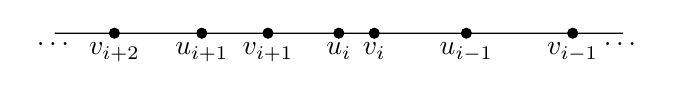
\begin{tikzpicture}[scale = 0.3]
\filldraw
(-12,0) circle (0.1pt) node[align=center, below] {$\dots$} --
(-9.5,0) circle (6pt) node[align=left,   below] {$v_{i+2}$} --
(-5.8,0) circle (6pt) node[align=center, below] {$u_{i+1}$} --
(-3,0) circle (6pt) node[align=left,   below] {$v_{i+1}$} --
(0,0) circle (6pt) node[align=left,   below] {$u_{i}$} --
(1.5,0) circle (6pt) node[align=left,   below] {$v_{i}$} --
(5.4,0) circle (6pt) node[align=center, below] {$u_{i-1}$} --
(9.9,0) circle (6pt) node[align=left,   below] {$v_{i-1}$} --
(12,0) circle (0.1pt) node[align=right,  below] {$\dots$};
\end{tikzpicture}

    \caption{Illustration of the interlacing of $\bm{u}$ on $\bm{v}$.}
    \label{f:Interlacing_eigenvalues}
\end{figure}

Let $k, d \in \mathbb{N}$, with $k \leq d$. Let $\bm{F} \in \mathbb{R}^{k \times d}$ be a full rank matrix\footnote{A \emph{frame}, using the definitions of \citep{FiMiPo11} and \citep{FMPS13}.}.
% We denote $b(\bm{F}), B(\bm{F}) \in \mathbb{R}_{+}$ the bounds of $\bm{F}$ as a frame, that are respectively the largest and the smallest non negative real numbers $b,B$ satisfying
% \begin{equation}
% \forall \bm{x} \in \mathbb{R}^{k},\: \: b \| \bm{x} \|^{2} \leq \sum\limits_{j \in [d]} (\bm{x}^{\Tran}\bm{f}_{j})^{2}  \leq B \| \bm{x} \|^{2}.
% \end{equation}
Within this section, we denote $\bm{\sigma}^2 = (\sigma_{1}^2, \sigma_{2}^2, \dots ,\sigma_{k}^2)$ the squares of the nonvanishing singular values of the matrix $\bm{F}$, and $\bm{\ell} = (\ell_{1}=\|\bm{f}_{1}\|^{2}, \ell_{2}=\|\bm{f}_{2}\|^{2}, \dots, \ell_{d}=\|\bm{f}_{d}\|^{2})$ are the squared norms of the columns of $\bm{F}$, which we assume to be ordered decreasingly:
$$\ell_{1} \geq \ell_{2} \geq \dots \geq \ell_{d}.$$
 When the rows of $\bm{F}$ are orthonormal, we can think of $\bm{\ell}$ as a vector of leverage scores.
 % We say that the frame $\bm{F}$ is tight if and only if $B(\bm{F}) = b(\bm{F})$.
\end{definition}
% We can prove easily that $b(\bm{F}) = \sigma_{min}(\bm{F})$ and $B(\bm{F}) = \sigma_{max}(\bm{F})$. Thus, a tight frame is proportional to an orthogonal matrix with the same dimensions.

We are interested in the problem of constructing a matrix $\bm{F}$ with orthonormal rows given its leverage scores.
\begin{problem}\label{prob:orthogonal_frame_existence}
Let $k,d \in \mathbb{N}$, with $k \leq d$, and let $\bm{\ell} \in \mathbb{R}_{+}^{d}$ such that $\sum\limits_{i =1}^{d} \ell_{i} = k$. Build a matrix $\bm{F} \in \mathbb{R}^{k\times d}$ such that
\begin{equation}
\Sp(\bm{F}^{\Tran}\bm{F}) = [\mathbb{1}_{k},\mathbb{0}_{d-k}],
\end{equation}
and
\begin{equation}
\Diag(\bm{F}^{\Tran}\bm{F}) = \bm{\ell}.
\end{equation}
\end{problem}
We actually consider here the generalization of Problem~\ref{prob:general_frame_existence} to an arbitrary spectrum.

\begin{problem}\label{prob:general_frame_existence}
Let $k,d \in \mathbb{N}$, with $k \leq d$, and let $\bm{\ell} \in \mathbb{R}_{+}^{d}$ such that $\sum\limits_{i =1}^{d} \ell_{i} = \sum\limits_{i = 1}^{k} \sigma_{i}^2$. Build a matrix $\bm{F} \in \mathbb{R}^{k\times d}$ such that
\begin{equation}
\Sp(\bm{F}^{\Tran}\bm{F}) = [\bm{\sigma}^2,\mathbb{0}_{d-k}] =:\bm{\hat\sigma}^2
\end{equation}
and
\begin{equation}
\Diag(\bm{F}^{\Tran}\bm{F}) = \bm{\ell}.
\end{equation}
\end{problem}

Denote by
\begin{equation}
\mathcal{M}_{(\bm{\ell},\bm{\sigma})} =  \{ \bm{M} \in \mathbb{R}^{d\times d}\text{ symmetric } \big/~  \Diag(\bm{M}) = \bm{\ell}, ~\Sp(\bm{M}) = \bm{\hat{\sigma}}^2\}.
\end{equation}
The non-emptiness of $\mathcal{M}_{(\bm{\ell},\bm{\sigma})}$ is determined by a majorization condition between $\bm{\ell}$ and $\hat{\bm{\sigma}}$, see Appendix~\ref{app:majorization} for definitions. More precisely, we have the following theorem.
\begin{theorem}[Schur-Horn]\label{thm:majorization_equivalence}
Let $k,d \in \mathbb{N}$, with $k \leq d$, and let $\bm{\ell} \in \mathbb{R}_{+}^{d}$. We have
\begin{equation}\label{eq:nonemptiness_majorization_equivalence}
\mathcal{M}_{(\bm{\ell},\bm{\sigma})} \neq \emptyset \Leftrightarrow \bm{\ell} \prec_{S} \hat{\bm{\sigma}}.
\end{equation}
\end{theorem}
%The r.h.s condition in the equivalence \eqref{eq:nonemptiness_majorization_equivalence} is satisfied in the case where $\bm{\sigma} = \mathbb{1}_{k}$ and $\bm{\ell} \in \mathbb{R}_{+}^{d}$ such that $\sum\limits_{i \in [d]} \ell_{i} = k$.
The proof by \cite{Hor54} of the reciprocal in Theorem~\ref{thm:majorization_equivalence} is non constructive. In the next section, we survey algorithms that output an element of $\mathcal{M}_{(\bm{\ell},\bm{\sigma})}$.

\subsection{Related work}
%  We recall some definitions and related work...

%We can prove easily, that $b(\bm{F}) = \sigma_{min}(\bm{F})$ and $B(\bm{F}) = \sigma_{max}(\bm{F})$.
%Thus, a tight frame is proportional to an orthogonal matrix with the same dimensions.
% The problem of generating frames with a given spectrum and a prescribed profile of leverage scores is equivalent to the problem generation of symmetric matrix with a prescribed diagonal and positive spectrum.
Several articles (\citealp{RaMa14}, \citealp{MaMaYu14}) in the randomized linear algebra community propose the use of non Gaussian random matrices to generate matrices with a fast decreasing profile of leverage scores (so-called \emph{heavy hitters}) without controlling the exact profile of the leverage scores.

\cite{DhHeSuTr05} showed how to generate matrices from $\mathcal{M}_{(\bm{\ell},\bm{\sigma})}$ using Givens rotations; see the algorithm in Figure~\ref{f:Algo_Givens}. The idea of the algorithm is to start with a frame with the exact spectrum and repeatedly apply orthogonal matrices (Lines 4 and 6 of Figure~\ref{f:Algo_Givens}) that preserve the spectrum while changing the leverage scores of only two columns, setting one of their leverage scores to the desired value. The orthogonal matrices are the so-called \emph{Givens rotations}.
% used in this algorithm leave invariant a $(d-2)$-dimensional subspace of $\mathbb{R}^{d}$ and they are precisely the Givens rotations defined in the following.
\begin{definition}
Let $\theta \in [0, 2\pi[$ and $i,j \in [d]$. The Givens rotation $\bm{G}_{i,j}(\theta) \in \mathbb{R}^{d \times d}$ is defined by????
% \begin{equation}
% %\left[
% \bm{G}_{i,j}(\theta)  = \begin{bmatrix}
%     1 & & & & & & & & & & \\
%      & \ddots  & & & & & & & & & \\
%      &  & 1 & & & & & & & &  \\
%      &  &  &  \cos(\theta)&  &  & & -\sin(\theta)& & & \\
%      &  &  &  & 1 &   & & & & & \\
%      &  &  &  &  & \ddots  & & & & & \\
%      &  &  &  &  &   & 1 & & & & \\
%      &  &  &  \sin(\theta)&  &  & & \cos(\theta)& & & \\
%      &  & & & & & & &1 & & \\
%      &   & & & & & & & &\ddots & \\
%      &  &  & & & & & & & & 1 \\
%     \end{bmatrix}.
% %\right]
% \end{equation}

\end{definition}




\begin{figure}[!ht]
\centerline{
\begin{algorithm}{$\Algo{GivensAlgorithm}\big(\bm{\ell},\bm{\sigma})$}\label{algo_givens}
%\vspace{-.1cm}
\Aitem $\bm{F} \longleftarrow \left[
\begin{array}{c|c}
\Diag(\bm{\sigma}) & \bm{0}
\end{array}
\right] \in \mathbb{R}^{k \times d}$
\Aitem \While $\exists i,j,k \in [d]$, $i < k <j: \|\bm{f}_{i}\|^{2} < \ell_{i}, \|\bm{f}_{k}\|^{2} = \ell_{k} , \|\bm{f}_{j}\|^{2} > \ell_{j}$
\Aitem \mt \If $\ell_{i} - \|\bm{f}_{i}\|^{2} \leq \|\bm{f}_{j}\|^{2} - \ell_{j}$
\Aitem \mtt $\bm{F}\setto \bm{G}_{i,j}(\theta)\bm{F}$, where  $\|(\bm{G}_{i,j}(\theta)\bm{F})_{i}\|^{2} = \ell_{i}$.
\Aitem \mt \Else
\Aitem \mtt $\bm{F}\setto \bm{G}_{i,j}(\theta)\bm{F}$, where $\|(\bm{G}_{i,j}(\theta)\bm{F})_{j}\|^{2} = \ell_{j}$,
\Aitem \Return $\bm{F} \in \mathbb{R}^{k \times d}$.
\end{algorithm}
}
\caption{The pseudocode of the algorithm proposed by \cite{DhHeSuTr05} for generating a matrix given its leverage scores and spectrum by successively applying Givens rotations.}
\label{f:Algo_Givens}
\end{figure}

Figure~\ref{f:highly_structured_matrix} shows the output of the algorithm in Figure~\ref{f:Algo_Givens}, for the input $(\bm{\ell},\bm{\sigma}) = (\bm{\ell},\mathbb{1})$ for three different values of $\bm{\ell}$. The main drawbacks of this algorithm are first that it is deterministic, so that it outputs a unique matrix $\bm{F}$ for a given input $(\bm{\ell},\bm{\sigma})$, and second that the output is a highly structured matrix, as observed on Figure~\ref{f:highly_structured_matrix}.

 We propose an algorithm that outputs random, more ``generic" matrices belonging to $\mathcal{M}_{(\bm{\ell},\bm{\sigma})}$. This algorithm is based on a parametrization of $\mathcal{M}_{(\bm{\ell},\bm{\sigma})}$ using the collection of spectra of all minors of $\bm{F} \in \mathcal{M}_{(\bm{\ell},\bm{\sigma})}$. This parametrization was introduced by \cite{FMPS13}, and we recall it in Section~\ref{s:gt}. For now, let us simply look at  Figure~\ref{f:gt_generator_outputs}, which displays a few outputs of our algorithm for the same input as in Figure~\ref{f:highly_structured_matrix:a}. We now obtain different matrices for the same input $(\bm{\ell},\bm{\sigma})$, and these matrices are less structured than the output of Algorithm~\ref{f:Algo_Givens}, as required.

\subsection{The restricted Gelfand-Tsetlin polytope}
\label{s:gt}
\begin{definition}
Recall that $(\bm{f}_{i})_{i \in [d]}$ are the columns of the matrix $\bm{F}\in\mathbb{R}^{k\times d}$. For $r \in [d]$, we further define
\begin{equation}
\bm{F}_{r} = \bm{F}_{:,[r]} \in \mathbb{R}^{k \times r},
\end{equation}
\begin{equation}
\bm{C}_{r} = \sum\limits_{i \in [r]} \bm{f}_{i}\bm{f}_{i}^{\Tran} \in \mathbb{R}^{k \times k},
\end{equation}
\begin{equation}
\bm{G}_{r} = \bm{F}_{r}^{\Tran}\bm{F}_{r} \in \mathbb{R}^{r \times r}.
\end{equation}
Furthermore, we note for $r \in [d]$,
\begin{equation}
    (\lambda_{r,i})_{i \in [k]} = \Lambda(\bm{C}_{r}),
\end{equation}
\begin{equation}
    (\tilde{\lambda}_{r,i})_{i \in [r]} = \Lambda(\bm{G}_{r}).
\end{equation}
The $(\lambda_{r,i})_{i \in [k]}$, $r\in [d]$, are called the outer eigensteps of $\bm{F}$, and we group them in the matrix $$\Lambda^{\text{out}}(\bm{F}) = (\lambda_{r,i})_{i \in [k],r \in [d]} \in \mathbb{R}^{k \times d}.$$ Similarly, the $(\tilde{\lambda}_{r,i})_{i \in [r]}$ are called inner eigensteps of $\bm{F}$: \rev{for $r \in [d]$, $(\lambda_{r,i})_{i \in [k]}$ and $(\tilde{\lambda}_{r,i})_{i \in [r]}$ share the same nonzeros elements.}
\end{definition}


\begin{figure}[!ht]
    \centering
\subfloat[]{\includegraphics[width= 0.25\textwidth]{img/cssp/toydatasets/givens_generator_d_10_k_2_sample_1.pdf}
\label{f:highly_structured_matrix:a}}
\subfloat[]{\includegraphics[width= 0.25\textwidth]{img/cssp/toydatasets/givens_generator_d_10_k_2_sample_2.pdf}}
\subfloat[]{\includegraphics[width= 0.25\textwidth]{img/cssp/toydatasets/givens_generator_d_10_k_2_sample_3.pdf}}
\caption{The output of the algorithm in Figure~\ref{f:Algo_Givens} for $k=2, \: d = 10$, $\bm{\sigma} = (1,1)$, and three different values of $\bm{\ell}$ that each add to $k$. Each red dot has coordinates a column of $\bm{F}$. The blue circles have for radii the prescribed $(\sqrt{\ell_i})$.
\label{f:highly_structured_matrix}}
\end{figure}

\begin{figure}[!ht]
    \centering
\subfloat[]{\includegraphics[width= 0.25\textwidth]{img/cssp/toydatasets/gt_generator_d_10_k_2_sample_1.pdf}}
\subfloat[]{\includegraphics[width= 0.25\textwidth]{img/cssp/toydatasets/gt_generator_d_10_k_2_sample_2.pdf}}
\subfloat[]{\includegraphics[width= 0.25\textwidth]{img/cssp/toydatasets/gt_generator_d_10_k_2_sample_3.pdf}}
\subfloat[]{\includegraphics[width= 0.25\textwidth]{img/cssp/toydatasets/gt_generator_d_10_k_2_sample_4.pdf}}\\
%\caption{The output of Algorithm \ref{algo_givens} for an input (k=2 d = 20)}
 %   \centering
\subfloat[]{\includegraphics[width= 0.25\textwidth]{img/cssp/toydatasets/gt_generator_d_10_k_2_sample_5.pdf}}
\subfloat[]{\includegraphics[width= 0.25\textwidth]{img/cssp/toydatasets/gt_generator_d_10_k_2_sample_6.pdf}}
\subfloat[]{\includegraphics[width= 0.25\textwidth]{img/cssp/toydatasets/gt_generator_d_10_k_2_sample_7.pdf}}
\subfloat[]{\includegraphics[width= 0.25\textwidth]{img/cssp/toydatasets/gt_generator_d_10_k_2_sample_8.pdf}}
\caption{The output of our algorithm for $k=2, \: d = 10$, an input $\bm{\sigma} = (1,1)$, and $\ell$ as in Figure~\ref{f:highly_structured_matrix:a}. Each red dot has coordinates a column of $\bm{F}$. The blue circles have for radii the prescribed $(\sqrt{\ell_i})$. \label{f:gt_generator_outputs}}
\end{figure}


% \begin{figure}
%     \centering
% \includegraphics[width= 0.9\textwidth]{img/inner_and_outer_eigensteps.png}

% \caption{The relationship between inner eigensteps and outer eigensteps.}
% \end{figure}

\begin{example}
For $k=2$, $d = 4$, consider the full-rank matrix
\begin{equation}
    \bm{F} = \begin{bmatrix}
1 & 0 & -1 & 0 \\
0 & 1 & 0 & -1
\end{bmatrix},
\end{equation}
Then
\begin{equation}
    \Lambda^{\text{out}}(\bm{F}) = \begin{bmatrix}
1 & 1 & 2 & 2 \\
0 & 1 & 1 & 2
\end{bmatrix}.
\end{equation}


\end{example}

\begin{proposition}
The outer eigensteps satisfy the following constraints:\\
\begin{equation}\label{eq:GT_polytope_equations}
\begin{cases}
     \forall i \in [k], \:\: \lambda_{0,i} = 0 \\
     \forall i \in [k], \:\: \lambda_{d,i} = \sigma_{i}^2 \\
     \forall r \in [d], \:\: (\lambda_{r,:}) \sqsubseteq  (\lambda_{r+1,:}) \\
     \forall r \in [d], \:\: \sum\limits_{i \in [d]} \lambda_{r,i} = \sum\limits_{i \in [r]} \ell_{i}
\end{cases}.
\end{equation}
\end{proposition}
% \begin{figure}
%     \centering
% \includegraphics[width= 0.9\textwidth]{img/Interlacing_eigenspaces.png}

% \caption{The interlacing relationships satisfied by the eigenspaces of a frame.}
% \end{figure}
\begin{figure}[!ht]
    \centering
    

\begin{tikzpicture}[scale = 0.3]

  % draw line and angle
%  \draw 
%     pic [draw,angle radius=4mm,angle eccentricity=1.5, "$\theta$" font=\scriptsize] {angle=v2--v1--v3};

 

%\draw [fill=blue, opacity=0.5] (-15,3.75) -- (-11,3.75) -- (-11,5.5) -- (-15,5.5) -- (-15,3.75);
%\draw [fill=blue, opacity=0.5] (-15,3.5) -- (-11,3.5) -- (-11,3.75) -- (-15,3.75) -- (-15,3.5);
%\draw [fill=blue, opacity=0.5] (-15,3.25) -- (-11,3.25) -- (-11,3.5) -- (-15,3.5) -- (-15,3.25);
%\draw [fill=blue, opacity=0.5] (-15,4) -- (-11,4) -- (-11,3.25) -- (-15,3.25) -- (-15,4);
%\draw [fill=blue, opacity=0.5] (-15,2.75) -- (-11,2.75) -- (-11,4) -- (-15,4) -- (-15,2.75); 
%\draw [fill=blue, opacity=0.5] (-15,2.5) -- (-11,2.5) -- (-11,2.75) -- (-15,2.75) -- (-15,2.5);
%\draw [fill=blue, opacity=0.5] (-15,2.25) -- (-11,2.25) -- (-11,2.5) -- (-15,2.5) -- (-15,2.25);
%\draw [fill=blue, opacity=0.5] (-15,2) -- (-11,2) -- (-11,2.25) -- (-15,2.25) -- (-15,2);
%\draw [fill=blue, opacity=0.5] (-15,1.75) -- (-11,1.75) -- (-11,2) -- (-15,2) -- (-15,1.75);



%\draw [fill=blue, opacity=1] (-2,3.75) -- (2,3.75) -- (2,5.5) -- (-2,5.5) -- (-2,3.75);
%\draw [fill=blue, opacity=1] (-2,3.5) -- (2,3.5) -- (2,3.75) -- (-2,3.75) -- (-2,3.5);
%\draw [fill=blue, opacity=0.5] (-2,3.25) -- (2,3.25) -- (2,3.5) -- (-2,3.5) -- (-2,3.25);
%\draw [fill=blue, opacity=0.5] (-2,4) -- (2,4) -- (2,3.25) -- (-2,3.25) -- (-2,4);
%\draw [fill=blue, opacity=1] (-2,2.75) -- (2,2.75) -- (2,4) -- (-2,4) -- (-2,2.75); 
%\draw [fill=blue, opacity=0.5] (-2,2.5) -- (2,2.5) -- (2,2.75) -- (-2,2.75) -- (-2,2.5);
%\draw [fill=blue, opacity=0.5] (-2,2.25) -- (2,2.25) -- (2,2.5) -- (-2,2.5) -- (-2,2.25);
%\draw [fill=blue, opacity=1] (-2,2) -- (2,2) -- (2,2.25) -- (-2,2.25) -- (-2,2);
%\draw [fill=blue, opacity=0.5] (-2,1.75) -- (2,1.75) -- (2,2) -- (-2,2) -- (-2,1.75);





%\draw [fill=blue, opacity=1] (13,2.75) -- (17,2.75) -- (17,4) -- (13,4) -- (13,2.75);
%\draw [fill=blue, opacity=1] (13,2.5) -- (17,2.5) -- (17,2.75) -- (13,2.75) -- (13,2.5);
%\draw [fill=blue, opacity=1] (13,2.25) -- (17,2.25) -- (17,2.5) -- (13,2.5) -- (13,2.25);
%\draw [fill=blue, opacity=1] (13,2) -- (17,2) -- (17,2.25) -- (13,2.25) -- (13,2);


%\draw [fill=orange, opacity=1] (13.25,2) -- (13.25,2) -- (13.5,2) -- (13.5,4) -- (13.25,4);
%\draw [fill=orange, opacity=1] (14.25,2) -- (14.25,2) -- (14.5,2) -- (14.5,4) -- (14.25,4);
%\draw [fill=orange, opacity=1] (14.75,2) -- (14.75,2) -- (15,2) -- (15,4) -- (14.75,4);
%\draw [fill=orange, opacity=1] (15.75,2) -- (15.75,2) -- (16,2) -- (16,4) -- (15.75,4);



%\draw [->] (-7.5,2) --  (-6.5,2)  node [above] {\tiny $\Prb(T) \propto \prod_{i \in T} \sigma_{i}^{2}$} --  (-5.5,2);

%\draw [->] (6.5,2) --  (7.5,2)  node [above] {\tiny $\Prb(S|T) = \Det (\bm{V}_{S,T})^{2}$} --  (11.5,2);

%\draw  (-17,2.25)  node [above] {$\bm{V}^{\Tran}=$} ;

\draw  (-40,7)  node  {$\ell_{1}=\lambda_{1,1}$} ;
\draw  (-36,7)  node  {$\newprec$} ;
\draw  (-32,7)  node  {$\lambda_{2,1}$} ;
\draw  (-28,7)  node  {$\newprec$} ;
\draw  (-24,7)  node  {$\lambda_{3,1}$} ;
%\draw  (-20,7)  node  {$\newprec$} ;
\draw  (-20,7)  node  {$\dots$} ;
\draw  (-16,7)  node  {$\lambda_{d-1,1}$} ;
\draw  (-12,7)  node  {$\newprec$} ;
\draw  (-8,7)  node  {$\lambda_{d,1} = \sigma_{1}$} ;


\draw  (-38.5,5.5)  node  {$\scriptscriptstyle +$} ;
\draw  (-36,5.5)  node  {$\newtiltedprec$} ;
%\draw  (-32,3.5)  node  {$a$} ;
\draw  (-32,5.5)  node  {$\scriptscriptstyle +$} ;
\draw  (-28,5.5)  node  {$\newtiltedprec$} ;
\draw  (-24,5.5)  node  {$\scriptscriptstyle +$} ;
%\draw  (-24,3.5)  node  {$a$} ;
\draw  (-20,5.5)  node  {$\dots$} ;
\draw  (-16,5.5)  node  {$\scriptscriptstyle +$} ;
%\draw  (-16,3.5)  node  {$a$} ;
%\draw  (-16,3.5)  node  {$a$} ;
\draw  (-12,5.5)  node  {$\newtiltedprec$} ;
\draw  (-8.7,5.5)  node  {$\scriptscriptstyle +$} ;




\draw  (-40,4)  node  {$0=\lambda_{1,2}$} ;
\draw  (-36,4)  node  {$\newprec$} ;
\draw  (-32,4)  node  {$\lambda_{2,2}$} ;
\draw  (-28,4)  node  {$\newprec$} ;
\draw  (-24,4)  node  {$\lambda_{3,2}$} ;
%\draw  (-20,7)  node  {$\newprec$} ;
\draw  (-20,4)  node  {$\dots$} ;
\draw  (-16,4)  node  {$\lambda_{d-1,2}$} ;
\draw  (-12,4)  node  {$\newprec$} ;
\draw  (-8,4)  node  {$\lambda_{d,2} = \sigma_{2}$} ;


\draw  (-38.5,2.5)  node  {$\scriptscriptstyle +$} ;
\draw  (-36,2.5)  node  {$\newtiltedprec$} ;
\draw  (-32,2.5)  node  {$\scriptscriptstyle +$} ;
\draw  (-28,2.5)  node  {$\newtiltedprec$} ;
\draw  (-24,2.5)  node  {$\scriptscriptstyle +$} ;
\draw  (-20,2.5)  node  {$\dots$} ;
\draw  (-16,2.5)  node  {$\scriptscriptstyle +$} ;
%\draw  (-16,3.5)  node  {$a$} ;
\draw  (-12,2.5)  node  {$\newtiltedprec$} ;
\draw  (-8.7,2.5)  node  {$\scriptscriptstyle +$} ;

\draw  (-40,1)  node  {$0=\lambda_{1,3}$} ;
\draw  (-36,1)  node  {$\newprec$} ;
\draw  (-32,1)  node  {$\lambda_{2,3}$} ;
\draw  (-28,1)  node  {$\newprec$} ;
\draw  (-24,1)  node  {$\lambda_{3,3}$} ;
%\draw  (-20,7)  node  {$\newprec$} ;
\draw  (-20,1)  node  {$\dots$} ;
\draw  (-16,1)  node  {$\lambda_{d-1,3}$} ;
\draw  (-12,1)  node  {$\newprec$} ;
\draw  (-8,1)  node  {$\lambda_{d,3} = \sigma_{3}$} ;


\draw  (-40,0)  node  {$\vdots$} ;
%\draw  (-36,0)  node  {$\newprec$} ;
\draw  (-32,0)  node  {$\vdots$} ;
%\draw  (-28,0)  node  {$\newprec$} ;
\draw  (-24,0)  node  {$\vdots$} ;
%\draw  (-20,7)  node  {$\newprec$} ;
\draw  (-20,0)  node  {$\vdots$} ;
\draw  (-16,0)  node  {$\vdots$} ;
%\draw  (-12,0)  node  {$\newprec$} ;
\draw  (-8,0)  node  {$\vdots$} ;



\draw  (-40,-1.5)  node  {$0=\lambda_{1,k}$} ;
\draw  (-36,-1.5)  node  {$\newprec$} ;
\draw  (-32,-1.5)  node  {$\lambda_{2,k}$} ;
\draw  (-28,-1.5)  node  {$\newprec$} ;
\draw  (-24,-1.5)  node  {$\lambda_{3,k}$} ;
%\draw  (-20,7)  node  {$\newprec$} ;
\draw  (-20,-1.5)  node  {$\dots$} ;
\draw  (-16,-1.5)  node  {$\lambda_{d-1,k}$} ;
\draw  (-12,-1.5)  node  {$\newprec$} ;
\draw  (-8,-1.5)  node  {$\lambda_{d,k} = \sigma_{k}$} ;

\draw[line width=0.15 mm] (-42,-2.5) -- (-3,-2.5);

\draw  (-38,-3.5)  node  {$\ell_{1}$} ;
\draw  (-36,-3.5)  node  {} ;
\draw  (-32,-4)  node  {$\sum\limits_{i \leq 2}\ell_{i}$} ;
\draw  (-28,-3.5)  node  {} ;
\draw  (-24,-4)  node  {$\sum\limits_{i \leq 3}\ell_{i}$} ;
%\draw  (-20,7)  node  {$\newprec$} ;
\draw  (-20,-3.5)  node  {} ;
\draw  (-16,-4)  node  {$\sum\limits_{i \leq d-1}\ell_{i}$} ;
\draw  (-12,-3.5)  node  {} ;
\draw  (-8.7,-4)  node  {$\sum\limits_{i \leq d}\ell_{i}$} ;
\end{tikzpicture}

    \caption{The interlacing relationships \eqref{eq:GT_polytope_equations} satisfied by the outer eigensteps of a frame. Thick triangles are used in place of $\leq$ for improved readability.}
    \label{f:Interlacing_eigenspaces}
\end{figure}

% \begin{figure}[!ht]
%     \centering
%     

\begin{tikzpicture}[scale = 0.3]


\draw  (-40,5)  node  {$\lambda_{1,1}$} ;
\draw  (-36,5)  node  {$\newprec$} ;
\draw  (-32,5)  node  {$\lambda_{2,1}$} ;

\draw  (-36,4)  node  {$\newtiltedprec$} ;




\draw  (-32,3)  node  {$\lambda_{2,2}$} ;


\end{tikzpicture}

%     \caption{The interlacing relationship between $\lambda_{1,1}$,$\lambda_{1,2}$ and $\lambda_{2,1}$: $\lambda_{2,2} \leq \lambda_{1,1} \leq \lambda_{2,1}$.
%     \label{f:Interlacing_eigenspaces}
%     }
% \end{figure}
In other words, the outer eigensteps are constrained to live in a polytope.
We define the restricted Gelfand-Tsetlin polytope $\bm{GT}_{(k,d)}(\bm{\sigma},\bm{\ell})$ to be the subset of $\mathbb{R}^{k \times d}$ defined by the equations \eqref{eq:GT_polytope_equations}. A more graphical summary of the interlacing and sum constraints is given in Figure~\ref{f:Interlacing_eigenspaces}. The restricted GT polytope\footnote{Note the difference with the Gelfand-Tsetlin polytope in the random matrix literature \citep{Bar01}, where only the spectrum is constrained, not the diagonal.} allows a parametrization of $\mathcal{M}_{(\bm{\ell},\bm{\sigma})}$ by the following reconstruction result.
% \begin{example}
% For $(k,d) = (2,5)$, we consider the frame
% \begin{equation}
%     \bm{F} = \begin{bmatrix}
% 1 & 1 & 1 & 1 & 1\\
% 1 & 1 & 1 & 1 & 1
% \end{bmatrix}
% \end{equation}
% we have
% \begin{equation}
%     \Lambda(\bm{F}) = \begin{bmatrix}
% 1 & 1 & 1 & 1 & 1\\
% 1 & 1 & 1 & 1 & 1
% \end{bmatrix}
% \end{equation}
% and

% \begin{equation}
%     \tilde{\Lambda}(\bm{F}) = \begin{bmatrix}
% 1 & 1 & 1 & 1 & 1\\
% 1 & 1 & 1 & 1 & 1
% \end{bmatrix}
% \end{equation}
% \end{example}

% \begin{figure}
%     \centering
% \includegraphics[width= 0.5\textwidth]{img/GT_polytope.png}

% \caption{The GT polytope for the frame ...}
% \end{figure}
\begin{theorem}[Theorem 3, \citealp{FiMiPo11}]\label{thm:GT_parameterization}
Every matrix $\bm{F}\in \mathcal{M}_{(\bm{\ell},\bm{\sigma})}$ can be constructed as follows:
\begin{itemize}
    \item pick a valid sequence of outer eigensteps noted $\Lambda^{\text{out}} \in \bm{GT}_{(k,d)}(\bm{\sigma},\bm{\ell})$,
    \item pick $\bm{f}_{1} \in \mathbb{R}^{k}$ such that
    \begin{equation}\label{eq:f_1_equation}
    \| \bm{f}_{1}\|^{2} = \ell_{1}
    ,\end{equation}
    \item for $r \in [d]$, consider the polynomial $p_{r}(x) = \prod\limits_{i \in [d]}(x - \lambda_{r,i})$, and for each $r \in [d-1]$, choose $\bm{f}_{r+1} \in \mathbb{R}^{k} $ such that
    \begin{equation}\label{eq:projections_of_f_on_eigenspaces}
        \forall \lambda \in \{\lambda_{r,i}\}_{i \in [d]} , \: \| \bm{P}_{r,\lambda}\bm{f}_{r+1}\|^{2} = -\lim\limits_{x \to \lambda}(x-\lambda)\frac{p_{r+1}(\lambda)}{p_{r}(\lambda)},
    \end{equation}
    where $\bm{P}_{r, \lambda}$ denotes the orthogonal projection onto the eigenspace $\Kerspace(\lambda \mathbb{I}_{k} - \bm{F}_{r}\bm{F}_{r}^{T})$.
\end{itemize}
Conversely, any matrix $\bm{F}$ constructed by this process is in $\mathcal{M}_{(\bm{\ell},\bm{\sigma})}$.

\end{theorem}
%heorem~\ref{thm:GT_parameterization} guarantees the existence of a frame for a given sequence of eigensteps $\Lambda^{\text{out}} \in \bm{GT}_{(k,d)}(\bm{\sigma},\bm{\ell})$.
\cite{FiMiPo11} propose an algorithm to construct a vector $\bm{f}_{r}$ satisfying Equation \eqref{eq:projections_of_f_on_eigenspaces}. Finally, an algorithm for the construction of a valid sequence of eigensteps $\Lambda^{\text{out}} \in \bm{GT}_{(k,d)}(\bm{\sigma},\bm{\ell})$ was proposed in \citep{FMPS13}. This yields the following constructive result.

\begin{theorem}[Theorem 4.1, \citealp{FMPS13}]\label{thm:parametrization_of_polytope}
Every matrix $\bm{F}\in\mathcal{M}({\bm{\sigma},\bm{\ell}})$ can be constructed as follows:
\begin{itemize}
    \item Set $\forall i \in [k], \: \tilde\lambda_{d,i} = \sigma_{i}^2$,
    \item For $r \in \{d-1, \dots, 1 \}$, construct $\{\tilde\lambda_{r,:}\}$ as follows. For each $i \in \{k, \dots , 1\}$, pick $$\tilde\lambda_{r-1,i} \in [B_{i,r}(\bm{\ell},\bm{\sigma}),A_{i,r}(\bm{\ell},\bm{\sigma})],$$ where
    \begin{equation}
    \begin{split}
      A_{i,r}(\bm{\ell},\bm{\sigma}) = \max \left\{\tilde\lambda_{r+1,i+1}, \sum\limits_{t = i}^{k}\tilde\lambda_{r+1,t} - \sum\limits_{t = i+1}^{k}\tilde\lambda_{r,t} - \ell_{r+1} \right\}\\
      B_{i,r}(\bm{\ell},\bm{\sigma}) = \min \left\{\tilde\lambda_{r+1,i}, \min\limits_{z = 1,\dots,i} \left\{\sum\limits_{t=z}^{r}\ell_{t} - \sum\limits_{t=z+1}^{i}\tilde\lambda_{r+1,t} - \sum\limits_{t=i+1}^{k}\tilde\lambda_{r,t}\right\} \right\}.
    \end{split}
    \end{equation}
  \end{itemize}
Furthermore, any sequence constructed by this algorithm is a valid sequence of inner eigensteps.
\end{theorem}

Based on these results we propose an algorithm for the generation of orthogonal random matrices with a given profile of leverage scores.

\subsection{Our algorithm}
We consider a randomization of the algorithm given in Theorem~\ref{thm:parametrization_of_polytope}.
First, we generate a random sequence of valid inner eigensteps $\Lambda^{\text{in}}$ using Algorithm~\ref{f:Algo_Random_Eigensteps}. Then we proceed to the reconstruction a frame that admits $\Lambda^{\text{in}}$ as a sequence of eigensteps using the Algorithm proposed in \citep{FiMiPo11}.

Note that Equations \eqref{eq:f_1_equation} and \eqref{eq:projections_of_f_on_eigenspaces} admit several solutions. For example, for $r \in [d]$, and if $\bm{f}_{r+1}$ satisfies \eqref{eq:projections_of_f_on_eigenspaces}, $-\bm{f}_{r+1}$ satisfies this equation too. \cite{FiMiPo11} actually prove that the set of solutions of these equations is invariant under a specific action of the orthogonal group $\mathbb{O}(\rho(r,k))$ where $\rho(r,k) \in \mathbb{N}$ nontrivially depends on the eigensteps. \rev{In the reconstruction step of our algorithm, we apply a random orthogonal matrix sampled from the Haar measure on $\mathbb{O}(d)$ to the vector $\bm{f}_{1}$ and, then, for every $r \in [2:d]$, we apply an independent random orthogonal matrix $\Omega$ to a vector $\bm{f}_{r+1}$, that satisfies \eqref{eq:projections_of_f_on_eigenspaces}, so that $\Omega \bm{f}_{r+1}$ still satisfies \eqref{eq:projections_of_f_on_eigenspaces}.}


% we apply an independent random orthogonal matrix sampled from the Haar measure on $\mathbb{O}(\rho(r,k))$ to each reconstructed vector $\bm{f}_{r+1}$.

Figure~\ref{f:gt_generator_outputs} displays a few samples from our algorithm, which display diversity and no apparent structure, as required for a generator of toy datasets. The question of fully characterizing the distribution of the output of our algorithm is an open question.
% In particular, we consider, for future work, the problem of generating uniform random matrices from the set $\mathcal{M}_{(\bm{\ell},\bm{\sigma})}$ using an adaptation of our algorithm.

\begin{figure}
\centerline{
\scalebox{1}{
\begin{algorithm}{$\Algo{RandomEigensteps}\big(\bm{\ell},\bm{\sigma})$}\label{algo_givens}
%\vspace{-.1cm}
\Aitem $\Lambda^{\text{out}} \longleftarrow \mathbb{O} \in \mathbb{R}^{k \times d}$
\Aitem $\forall i \in [k], \: \tilde\lambda_{d,i} \longleftarrow \sigma_{i} $
\Aitem \For $r \in \{d-1,\dots,1 \}$
\Aitem \mt \For $i \in \{k,\dots,1 \}$
\Aitem \mtt Pick $\tilde\lambda_{r-1,i} \sim \mathcal{U}([B_{i,r}(\bm{\ell},\bm{\sigma}),A_{i,r}(\bm{\ell},\bm{\sigma})])$\\
\Return $\Lambda^{\text{out}}$
\end{algorithm}
}
}
\caption{The pseudocode of the generator of random valid eigensteps taking as input $(\bm{\ell},\bm{\sigma})$.}
\label{f:Algo_Random_Eigensteps}
\end{figure}
%\clearpage

\chapter{Kernel quadrature using DPPs}\label{chap:dppkq}
\section{Introduction}
Numerical integration is at the heart of many tasks in applied mathematics and statistics, like Bayesian inference \citep{RoCa04}, option pricing \citep{Gla13} or solving integral equations \citep{KrMaKo89}. Indeed, all these tasks involve, at some level, the evaluation of an integral
\begin{equation}\label{eq:general_integral_formula}
\int_{\mathcal{X}}f(x)\mathrm{d}\omega(x).
\end{equation}

Integrals that can be written in closed form are the exception; in general the value of~\eqref{eq:general_integral_formula} is only known through approximations. The problem of approximating an integral find its roots in an older problem:
the evaluation of the perimeter or the area of a domain bounded by curves. For example, the problem of squaring a circle occupied minds for centuries. By approximating a circle by a union of squares, a first estimation of $\pi \approx 256/81 \approx 3.1605$ was already known by Egyptians as it can be witnessed by the Rhind papyrus \citep{RoSh87}. Archimedes achieved a better approximation of the value of $\pi$ by computing the perimeter of the regular 96-gons and obtained \citep{Hea03}
$$3+\frac{10}{71} < \pi < 3+\frac{1}{7}.$$

% inscribed and circumscribed of ,   [???] 

 These geometric techniques were further developed after the invention of calculus. For instance, Newton considered the approximation of the integral of a function $f$ on some interval $[a,b]$ using some evaluations of $f(x_{1}), \dots, f(x_{N})$ of $f$
\begin{equation}
\int_{a}^{b}f(t)\mathrm{d}t \approx \sum\limits_{n \in [N]}w_{n}f(x_{n}).
\end{equation}
 In modern words, his approach goes as follows: evaluate $f$ on equally distanced nodes $x_{1}, \dots, x_{N}$ and consider the interpolating polynomial $p_{N-1}$

 % $p_{N-1}$ of $f$ on the $x_{1}, \dots, x_{N}$ then approximate the value of $\displaystyle \int_{a}^{b}f(t)\mathrm{d}t$ by $\displaystyle \int_{a}^{b}p_{N-1}(t)\mathrm{d}t$. In other words, consider the polynomial

  % Newton was interested in approximation   using some evaluations of $f$ can be tracked to the work of Newton. The idea of the eponymous quadrature is to consider a set of nodes, also called \emph{configuration}, $\bm{x} = \{x_{1}, \dots , x_{N} \} \subset \X^{N}$, and the corresponding interpolating polynomial of degree $N-1$:
\begin{equation}
p_{N-1}(t) = \sum\limits_{n \in [N]} f(x_{n}) \ell_{n,\bm{x}}(t) \in \mathbb{R}_{N-1}[t],
\end{equation}
where $\ell_{n,\bm{x}}$ are the Lagrange polynomial  \footnote{ At that time, Newton considered divided differences interpolation polynomial \citep{BuFa97}.} basis polynomials defined by \citep{BuFa97}
\begin{equation}
\ell_{n,\bm{x}}(t) = \frac{\prod\limits_{m \in [N], m \neq n }(t-x_{m})}{\prod\limits_{m \in [N], m \neq n }(x_{n}-x_{m})}.
\end{equation}
Newton then approximates the integral of $f$ by that of $p_{N-1}$
% The approximation of Newton writes
\begin{align}\label{eq:Newton_Cotes}
\int_{a}^{b}f(t)\mathrm{d}t & \approx  \sum\limits_{n \in [N]}w_{n}f(x_{n})  ,
\end{align}
where the scalars $w_{n}$, also called the \emph{Cotes numbers}, have the expression
\begin{equation}
\forall n \in [N], \: w_{n} = \int_{a}^{b} \ell_{n,\bm{x}}(t) \mathrm{d}t.
\end{equation}

The approximation~\eqref{eq:Newton_Cotes}, called the \emph{Newton-Cotes formula}, is an early form of a \emph{quadrature}: the nodes $x_{n}$ and the weights $w_{n}$ are independent of the function $f$. In the case of the Newton-Cotes formula, the explicit values of the weights, for small values of $N$, were found by Cotes. This formula coincides with other well-known quadratures such as the Trapezoid rule, the Simpson's rule, the Boole's rule... Nevertheless, this formula is not optimal for large values of $N$ and the nodes should be replaced by other configurations. This observation gave birth to the Gaussian quadrature and the field of numerical integration using the zeros of orthogonal polynomials.
 % The explicit values of the weights $w_{n}$ wIn the case of the \emph{Newton-Cotes formula}, the explicit values of the weights $w_{n}$ were calculated by Cotes for small values of $N$.
As we shall see, these techniques are not amenable to be generalized for  high-dimensional domains.

Monte Carlo methods offer another approach to numerical integration. This class of methods, introduced by \cite{MeUl49},  relies on randomized averaging. Given a sequence of random variables $x_{1}, \dots, x_{N}$ generated from a density g with respect to $\mathrm{d}\omega$, it comes
\begin{equation}
\EX \frac{1}{N}\sum\limits_{n \in [N]} f(x_{n}) = \int_{\mathcal{X}} f(x)g(x) \mathrm{d}\omega(x),
\end{equation}
and by the Strong Law of Large Numbers, $ \sum_{n \in [N]} f(x_{n})/N$ converges ($N \rightarrow +\infty$) a.s. to $\displaystyle \int_{\mathcal{X}} f(x)g(x) \mathrm{d}\omega(x)$. Moreover, if $\displaystyle \int_{\mathcal{X}} f(x)^{2} \mathrm{d}\omega(x) < +\infty$, the variance of $\sum_{n \in [N]} f(x_{n})/N$ scales as $\mathcal{O}(1/N^{2})$, and the estimator satisfies a central limit theorem \citep{RoCa04}. 
Remarkably, this rate of convergence does not depend on the dimension of $\mathcal{X}$ (if $\mathcal{X}$ is a $d$-dimensional manifold). This property gives an advantage of Monte Carlo methods over deterministic quadrature rules, that scales poorly for high dimension integration problems. 

It would be fair to claim that deterministic quadratures are very efficient for smooth low dimensional functions, while this smoothness does not improve the Monte Carlo rate. This observation have fueled a multitude of investigations with a common purpose: improving upon the Monte Carlo rate for smooth functions on high dimensional integration problems. Many approaches were proposed in this rich line of research: Quasi-Monte Carlo methods \citep*{DiPi10}, kernel quadrature methods \citep*{Hic98} \citep{SmGrSoSc07} \citep{ChWeSm10}, control functional techniques \citep*{OaGi16} or  determinantal point processes \citep{BaHa16}.

In this chapter a brief review of existing numerical integration methods is given with an emphasis on the connections between these methods. In particular, the contribution of this chapter is the introduction of a new class of quadratures that is at the intersection between determinantal point process and kernel quadrature methods.



\section{Related work}
The purpose of this section is to motivate the definition and the theoretical analysis of a class of quadratures based on projection DPPs. This class of quadratures is naturally defined within the RKHS framework. The merit of this class of quadratures is its universality and applicability to a variety of settings. An exhaustive review of existing results on quadratures is outside the scope of this manuscript; nevertheless, it turns out that many landmark quadratures are relevant to the contribution of this chapter. 
Thus, it is the purpose of this section to highlight these connections.



% More importantly, the connexions between projection DPPs and existing work on quadratures is highlighted. 


% For this purpose, we review existing results on quadratures 


\subsection{Gaussian quadrature}\label{sec:Gaussian_quadrature}
As we have seen in the introduction, the Newton-Cotes formula is based on equi-distanced nodes on $[a,b]$ and it is exact for polynomials of order smaller than $N-1$ when $N$ nodes are used. Gauss \citep{Gau1815} observed that equi-distance nodes are not optimal, in a sense that will be defined later, and shed the light on the question of designing the quadrature nodes. This observation gave birth to Gaussian quadrature.
% We start by a brief review on quadratures on the real line.
% \subsubsection{Newton-Cotes quadrature}

\subsubsection{The construction}

 Gauss investigated the maximal order of exactness that could be achieved by a quadrature rule based on a configuration of nodes $\bm{x} = \{ x_{1}, \dots, x_{N} \}$ and the corresponding weights $w_{1}, \dots, w_{N}$. This order is defined by 

\begin{equation}
M(\bm{x}) = \sup \bigg\{ M \in \mathbb{N}; \exists \bm{w} \in \mathbb{R}^{N}, \: \forall m \in [M], \: \int_{a}^{b} t^{m} \mathrm{d}t = \sum\limits_{n \in [N]} w_{n}x_{n}^{m} \bigg\}.
\end{equation}


%  that the $M(\bm{x}) \geq N-1$ for any proper design $\bm{x}$

% Gauss dealed with the maximal order of exactness in the Newton-Cotes quadrature:\\

% \emph{For a fixed value $N$, what is the maximal order $M(\bm{x})$ of polynomials such that the approximation \eqref{eq:Newton_approx} is exact?}

He proved that for any positive integer $N$ there exists a unique configuration $\bm{x}_{G}$, also called the \emph{Gauss nodes}, of cardinality $N$ such that $M(\bm{x}_{G}) = 2N-1$. He also proved that $2N-1$ is the maximal order that could be achieved by any configuration of cardinality $N$. His proof \citep{Gau1815} is based on arguments from continued fractions theory \citep{Khi97}.
% In particul there exists a remarkable design of nodes that achieves a higher degree of exactness: the approximation \eqref{eq:Newton_approx} is exact if $f$ is a polynomial of order less than $2N-1$.
% An alternative proof was given by Jacobi , where he proved the existence of this optimal configuration using . 
Later, \cite{Jac1826} showed, using an alternative proof based on simple manipulations on polynomials, that $M(\bm{x}) = 2N-1$ if and only if for every polynomial $p$ of order smaller or equal to $N-1$

\begin{equation}\label{eq:Legendre_orthogonality}
\int_{a}^{b} p(t) \pi_{\bm{x}}(t) \mathrm{d}t = 0,
\end{equation}
where $\pi_{\bm{x}}$ is the polynomial
\begin{equation}
\pi_{\bm{x}}(t) = \prod\limits_{n \in [N]}(t-x_{n}).
\end{equation}
% that for any integer $N' \in [N]$, 

% the Newton-Cotes quadrature has the maximal degree of exactness $M(\bm{x}) = N-1+N'$ if and only if for every polynomial $p$ of order less than $N'-1$:

% The case $N' = N$ leads to the Gauss formula of maximal degree of exactness $2N-1$.

 In other words, the Gauss nodes are the roots of a polynomial of degree $N$ that satisfy the condition~\eqref{eq:Legendre_orthogonality} for every polynomial of degree less than $N-1$: the polynomial $\pi_{\bm{x}}$ is nothing else but the scaled Legendre polynomial of degree $N$.
%  In other words, the work of Jacobi highlighted the importance of orthogonality 
% between polynomials, with respect to the scalar product defined by $\mathrm{d}t$, in the construction of the Gauss nodes. Since then, several 
 This characterization \eqref{eq:Legendre_orthogonality} of the Gauss nodes highlighted the importance of the orthogonality between polynomials with respect to $\mathrm{d}t$ and motivated the extension of Gaussian quadrature to weighted measures, that is approximating
  % $\mathrm{d}\omega = w(t) \mathrm{d} t$ 

\begin{equation}
\int_{a}^{b}f(t)\mathrm{d}\omega(t) \approx \sum\limits_{n \in [N]} w_{n}f(x_{n}).
\end{equation}

% : $\mathrm{d}\omega$ is the Stieltjes measure associated to a non-decreasing function $\omega: \mathbb{R} \rightarrow \mathbb{R}$ with infinitely many points of increase.

In particular, \cite{Chr1877} generalized the Gauss-Jacobi construction to 
measures $\mathrm{d}\omega(t) = \omega(t)\mathrm{d}t$ for arbitrary weight functions $\omega$ and his approach is generalizable to even a broader class of measures \citep{Sze39}. Typically, $\mathrm{d}\omega$ is assumed to have finite moments of all orders, so that the orthonormal polynomials with respect to $\mathrm{d}\omega$ are well defined by
\begin{align}
\forall m \in \mathbb{N}, \: \mathrm{deg} P_{m} & = m, \\
\forall m,m' \in \mathbb{N}, \: \int_{a}^{b} P_{m}(t)P_{m'}(t) \mathrm{d}\omega(t) & = \delta_{m,m'}.
\end{align}
Again, the roots $x_{1}, \dots, x_{N}$ of $P_{N}$ achieve the maximal order $2N-1$ and the corresponding weights, 
% the nodes of the quadrature are the roots of the $N$-th orthonormal polynomial 
% The corresponding weights have the expression
% % By generalizing the argument of Jacobi, Christoffel proved that for every $N \in \mathbb{N}^{*}$ and the corresponding weights $w_{n}^{GC}$
% \begin{equation}
%  \:\: w_{n}^{GC} = \int_{a}^{b} \frac{\prod\limits_{m \in [N], m \neq n }(t-x_{m})}{\prod\limits_{m \in [N], m \neq n }(x_{n}-x_{m})} \mathrm{d}\omega(t),
% \end{equation}
called the \emph{Christoffel numbers}, satisfy the identity \citep{Sho29} (see also Theorem 3.4.2 in \citep{Sze39}): 
\begin{equation}\label{eq:w_n_christoffel_number_formula}
w_{n} = \frac{1}{\sum\limits_{m =0}^{N-1} P_{m}(x_{n})^{2}}. 
\end{equation}
Observe that in \eqref{eq:w_n_christoffel_number_formula}, every $w_{n}$ depends only on the corresponding node $x_{n}$: the Christoffel numbers are the evaluations of  
the so-called \emph{Christoffel function} at the roots of $P_{N}$. This function has an interesting interpretation in approximation theory that will be recalled in Chapter~\ref{chapter:signal_reconstruction}.


% defines a quadrature such that $\displaystyle \sum\limits_{n \in [N]} w_{n} f(x_{n})$ coincides with $\displaystyle  \int_{a}^{b} f(t) \mathrm{d}\omega(t)$ for every polynomial of degree smaller than $2N-1$. The weights of this quadrature 
%\subsubsection{Jacobi matrices}
 %goes through the evaluation the sequences of
In practice, the evaluation of the nodes and weights of Gaussian quadrature for a given measure $\mathrm{d}\omega$ relies on  the three-term recurrence coefficients associated to the polynomials $P_{m}$
\begin{align}\label{eq:OP_reccurence_1}
\forall m \in \mathbb{N}, \:\:t P_{m}(t) & = \sqrt{b_{m+1}}P_{m+1}(t) + a_mP_{m}(t) + \sqrt{b_{m}}P_{m-1}(t),\\
\label{eq:OP_reccurence_2}
t P_{0}(t) & = a_{0}P_{1}(t) + \sqrt{b_{0}}P_{0}(t) .
\end{align}
% As for now, we recall a spectral characterization of the Gaussian quadrature. 
% % In practice, the nodes and the weights of the Gaussian quadrature can be calculated using a more elegant way.
% For this purpose, denote by $(a_{m})_{m \in \mathbb{N}}$ and $(b_{m})_{m \in \mathbb{N}}$  
Indeed, let $J_{N}$ the tridiagonal matrix of order $N$ defined by
\begin{equation}
J_N = \left( \begin{array}{cccc}
a_{1} & \sqrt{b_{1}} & & 0\\
\sqrt{b_{1}} & \ddots & \ddots & \\
& \ddots & \ddots & \sqrt{b_{N-1}} \\
0 & & \sqrt{b_{N-1}} & a_{N} \end{array} \right).
\end{equation}
The roots of the $P_{N}$ are the eigenvalues of the tridiagonal matrix $J_{N}$, and for every eigenvalue $x$ the corresponding eigenvector is the vector $\big(P_{0}(x), \dots, P_{N-1}(x) \big)^{\Tran}$; see Theorem 2.13 in \citep{GoMe09}. In other words, the spectral decomposition of the Jacobi matrix gives the nodes and the weights of the Gaussian quadrature. The matrix $J_{N}$ is known explicitly for many classic orthogonal polynomials such as Chebyshev, Legendre, Hermite... Building up this matrices amount to the calculation of the moments of the measure $\mathrm{d}\omega$ which is a non trivial task for a general measure $\mathrm{d}\omega$. We refer to \citep{GoMe09} for more details on the algorithmic construction of Gaussian quadrature.


% a re-writing of \eqref{eq:OP_reccurence_1} and \eqref{eq:OP_reccurence_2} yields 

% \begin{equation}\label{eq:matrix_OP_reccurence}
% J_{N} \begin{pmatrix}
% P_{0}(t)  \\
% \vdots \\
% P_{N-1}(t) \\
% \end{pmatrix} = t \begin{pmatrix}
% P_{0}(t)  \\
% \vdots \\
% P_{N-1}(t) \\
% \end{pmatrix} - \begin{pmatrix}
% 0  \\
% \vdots \\
% a_{N-1}P_{N}(t) \\
% \end{pmatrix}, \:\: t \in \mathbb{R},
% \end{equation}
% where 


% From \eqref{eq:matrix_OP_reccurence}, we conclude that the roots of $P_{N}$ are the eigenvalues of the tridiagonal matrix $J_{N}$, and for every eigenvalue $x$ the corresponding eigenvector is the vector $\begin{pmatrix}
% P_{0}(x)  \\
% \vdots \\
% P_{N-1}(x) \\
% \end{pmatrix}$
\subsubsection{A connection with DPP}

\begin{figure}[]
    \centering
% \includegraphics[width= 0.45\textwidth]{img/neurips/Hermite/HermiteOP_kernel_diagonal}~
% \caption{..... \label{fig:diagonalHermiteEnsemble}}
% \end{figure}
% \begin{figure}[]
%     \centering
\includegraphics[width= 0.45\textwidth]{img/neurips/Hermite/HermiteOP_kernel_diagonal_N_5_vs_50000_empirical}~
\includegraphics[width= 0.45\textwidth]{img/neurips/Hermite/HermiteOP_kernel_diagonal_N_10_vs_50000_empirical}
\caption{The histogram of the eigenvalues of $\tilde{J}_{N}$ based on 50000 realizations compared to the first intensity function of the projection DPP eigenvalues of $J_{N}$ (the red dots)  with $N \in\{5,10\}$.   \label{fig:unidimHermiteEnsembleChristoffel}}
\end{figure}

We illustrate the construction of Gaussian quadrature based on the spectral decomposition of the matrix $J_N$ using the case of the Gaussian measure on the real line. The aim of this illustration is to highlight a connection between Gaussian quadrature and DPPs.

Now, let $\mathrm{d}\omega(t) = \omega(t) \mathrm{d}t$ be the Gaussian measure on $\mathbb{R}$ 
\begin{equation}
\omega(t) = \frac{1}{\sqrt{2\pi}} e^{-t^{2}/2}.
\end{equation}
 % through  in the case of  This illustration will and we 
It is well known, that the corresponding orthonormal polynomials are proportional to the probabilists Hermite polynomials, and the corresponding Jacobi matrix writes
% \begin{equation}
% H_{n}(t) = (-1)^{n}e^{t^{2}/2}\frac{\mathrm{d}^{n}}{\mathrm{d}t^{n}} e^{-t^{2}/2}
% \end{equation}

%  defines a sequence of orthogonal polynomials with respect to $\mathrm{d}\omega$ the corresponding family of orthonormal polynomials, .... In this case
\begin{equation}
J_N = \left( \begin{array}{cccc}
0 & \sqrt{N} & & 0\\
\sqrt{N} & \ddots & \ddots & \\
& \ddots & \ddots & \sqrt{N} \\
0 & & \sqrt{N} & 0 \end{array} \right).
\end{equation}
Now consider the following random matrix
\begin{equation}
\tilde{J}_N = \left( \begin{array}{cccc}
\mathcal{N}(0,1) & \chi_{(N-1)} & & 0\\
\chi_{(N-1)} & \ddots & \ddots & \\
& \ddots & \ddots & \chi_{1} \\
0 & & \chi_{1} & \mathcal{N}(0,1) \end{array} \right),
\end{equation}

where $\mathcal{N}(0,1)$ is a random variable that follows the standard normal distribution, and $\chi_{n}$ is a random variable that follows the chi distribution with $n$ degrees of freedom.
% In particular
% \begin{equation}
% \EX \tilde{J}_N = J_N.
% \end{equation}
It is well known that eigenvalues $\{x_{1}, \dots, x_{N} \}$ of $\tilde{J}_{N}$ have the following density \citep{DuEd05}

\begin{equation}\label{eq:J_tilde_eigenvalue_distribution}
(x_{1}, \dots, x_{N}) \propto \prod\limits_{n =1}^{N}e^{-x_{n}^{2}/2} \prod\limits_{1 \leq n<n' \leq N}  |x_{n}-x_{n'}|^{2}.
\end{equation}
Observe that
\begin{equation}
\EX \tilde{J}_N = J_N.
\end{equation}
From~\eqref{eq:J_tilde_eigenvalue_distribution}, we can prove that the eigenvalues of $\tilde{J}_{N}$ form a DPP of marginal kernel 
\begin{equation}
\kappa(x,y) = \sum\limits_{n=0}^{N-1} P_{n}(x)P_{n}(y),
\end{equation}
and the $\mathrm{d}\omega$ as a reference measure.

% On the other hand, assume that the $(\psi_{n})$ are the family of orthonormal polynomials with respect to $\mathrm{d}\omega$. Let $x \in \mathcal{X}$ and $\bm{x}$ a random subset of $\mathcal{X}^{N}$ drawn from the Projection DPP $(\KDPP, \mathrm{d}\omega)$, then
% \begin{equation}
% \Prb_{\DPP}(x \in \bm{x}) = \frac{1}{N}\KDPP(x,x)\mathrm{d}\omega(x) = \frac{1}{N}\sum\limits_{n \in [N]} \psi_{n}(x)\psi_{n}(x) \mathrm{d}\omega(x)= \frac{1}{NC_{N,\mathrm{d}\omega}(x)} \mathrm{d}\omega(x).
% \end{equation}
% In other words, the inclusion probability of the corresponding projection DPP is related to the inverse of the Christoffel function as defined in \eqref{eq:Christoffel_functions_definition}. 


Figure \ref{fig:unidimHermiteEnsembleChristoffel} shows the histogram of the eigenvalues of the matrix $\tilde{J}_N$ with $N \in \{5,10 \}$ calculated over 50000 realizations of $\tilde{J}_N$ compared to the first intensity function of the projection DPP defined by the kernel $\kappa$ and the reference measure $\mathrm{d}\omega$. We observe that the histogram matches the first intensity function that have local maxima around the eigenvalues of the matrix $J_{N}$ (the red dots), that are the scaled roots of probabilistic Hermite polynomial of degree $N$.
% the evaluations of the inclusion probability of the projection DPP in the case of RKHS  Recall that in this case the eigenfunctions are given by
% \begin{equation}
% \tilde{e}_{m}(.) = H_{m}(\sqrt{2c}.).
% \end{equation}
In other words, in this case, the projection DPP can be seen as a probabilistic relaxation of Gaussian quadrature. 

This case is far from being anecdotal. Indeed, this probabilistic relaxation is possible for Gaussian quadrature of other measures, and the resulting point process coincides with a projection DPP; see ???? for details on this topic.
% The theoretical analysis of these local maxima was carried out in . More precisely, the authors studied the approximations of those bumps by Gaussians centred on the Hermite polynomials roots, see Figure \ref{fig:unidimHermiteEnsembleChristoffel} (b).

 % In other words, the quadratures based on nodes sampled according to a projection DPP are probabilistic relaxations of classical quadratures based on roots of orthogonal polynomials that can be defined even if $N$ is not the square of an integer (the cases $N \in \{17,21\}$ in Figure~\ref{fig:HermiteEnsembleChristoffel}).


\subsubsection{The convergence rates}


In general, the integrand $f$ is not a polynomial of low degree so that the quadrature is not exact. One would expect to give a control of the remainder 
\begin{equation}
R_{\bm{x},\bm{w}} [f] = \int_{a}^{b}f(t)\mathrm{d}t - \sum\limits_{n \in [N]} w_{n}f(x_{n}),
\end{equation}
if the function $f$ is well approximated by low degree polynomials. This is the case of analytic functions for which $|R_{\bm{x},\bm{w}}| = \mathcal{O}(\alpha^{N})$ for some $\alpha \in ]0,1[$. For functions of limited degree of smoothness, Taylor series with integral remainder can be used to give an upper bound on the integration error $|R_{\bm{x},\bm{w}}|$ that scales as $\mathcal{O}(N^{-s})$ for some $s >1$ that depends on the smoothness of the function $f$. See Chapter 4 of \citep{DavRab84} for details on this topic. 

% the quadrature is guaranteed to converge at least at a polynomial rate 





%  This is the case of holomorphic functions for which a considerable amount of research was devoted; see Section 4.6 in . In particular  Now,  who introduced kernels $K_{N}$ so that the remainder of the quadrature writes
% \begin{equation}\label{eq:peano_identity}
% \int_{a}^{b}f(t)\mathrm{d}t - \sum\limits_{n \in [N]} w_{n}f(x_{n}) = \int_{a}^{b}K_{N}(t)f^{(s)}(t)\mathrm{d}t,
% \end{equation}
% where $f$ is assumed to have a piecewise continuous derivative of order $N$; and the kernel $K_{N}$ have the following expression
% \begin{equation}
% K_{N}(t) = R_{\bm{x},\bm{w}} \bigg[ \frac{\max(.-t,0)^{N-1}}{(N-1)!} \bigg].
% \end{equation}
% Peano's representation can be used in different ways to give an upper bound of the absolute value of the remainder. For example, \eqref{eq:peano_identity} yields
% \begin{equation}
% \bigg|\int_{a}^{b}f(t)\mathrm{d}t - \sum\limits_{n \in [N]} w_{n}f(x_{n}) \bigg| \leq \max\limits_{t \in [a,b]} |f^{(s)}(t)| \int_{a}^{b}|K_{N}(t)|\mathrm{d}t
% \end{equation}

% This technique is valid only when the integrand $f$ is sufficiently smooth....

% An alternative approach  

% This is the idea behind a technique developed by Peano who introduced a class of kernels $K_{s}$ so that the remainder of the quadrature writes
% \begin{equation}
% \int_{a}^{b}f(t)\mathrm{d}t - \sum\limits_{n \in [N]} w_{n}f(x_{n}) = \int\limits_{a}^{b}K_{s}(t)f^{(s)}(t)\mathrm{d}t,
% \end{equation}
% where $f$ is assumed to have a piecewise continuous derivative of order $s$; and the kernel $K_{s}$ have the following expression
% \begin{equation}
% K_{s}(t) = R_{\bm{x},\bm{w}} \bigg[ \frac{\max(.-t,0)^{s-1}}{(s-1)!} \bigg].
% \end{equation}


%  where only low-order derivatives of  one could use the Peano representation of the remainder ****


% Since any polynomial of degree smaller or equal to $N-1$ is equal to its $N-1$-degree interpolant polynomial, the approximation \eqref{eq:Newton_approx} is exact if $f$ is a polynomial of order smaller or equal to $N-1$. 


\subsubsection{Gaussian quadrature in high dimension domains}


Finally, there were many attempts to extend Gaussian quadrature to high dimensional domains using common zeros of multidimensional orthogonal polynomials; see \citep{Xu94} for details on this topic. For example, the construction of a high dimensional Gaussian quadrature would require to work with block Jacobi matrices instead of tridiagonal Jacobi matrices \citep{Xu94b}. However, this line of research is not developed yet from an algorithmic point of view.

% this class of quadrature are it seems that there is no satisfactory algorithmic toolbox for 


 




\subsection{Quasi-Monte Carlo methods}
As we have seen previously, a high precision approximation of a unidimensional integral  is possible using deterministic rules such as Newton-Cotes or Gaussian quadrature provided that the integrand is a polynomial or well approximated by a polynomial. Now, for a smooth function defined on some high-dimensional domain, one can use the tensor product of these rules. However, for a given error, the number of required integrand evaluations grows exponentially with the dimension $d$. This poor scalability of grids with respect to the dimension $d$ motivated the emergence of a new class of quadratures called quasi-Monte Carlo rules: they are based on "well-spread" low discrepancy sequences and their weights are uniform $w_{n} = 1/N$.

% These rules can be used for a high dimensional integral


% several quadrature rules are known for functions defined on the real line

% Until now, there is no theory that extend  Gaussian quadratures to high dimensional domains.   


% Quasi-Monte Carlo methods were introduced 

%  several quadrature rules are known for functions defined on the real line. The situation is far more complicated for integration problems in high-dimension. For instance, the uniform grid in the hypercube $[0,1]^{d}$ suffers from the "curse of the dimension": in an informal way, the rate of convergence are typically $\mathcal{O}(N^{-s/d})$ where $s$ is a regularity parameter; so that the required number of nodes necessary to get an integration error lower than some level $\epsilon$ scales as $\epsilon^{1/d}$. 



 
\subsubsection{The discrepancy functions and Koksma-Hlawka inequalities}

\begin{figure}
\centering
\includegraphics[width= 0.55\textwidth]{img/discrepancy/local_discrepancy.pdf}
\caption{The local discrapancy of a configuration $\bm{x}$ depends on the set $[\bm{0},u]$. \label{fig:local_discrepancy}}
\end{figure}

 A discrepancy function of a configuration $\bm{x} = \{x_{1}, \dots, x_{N} \} \subset \X$ quantifies the uniformity of the nodes of $\bm{x}$ in $\mathcal{X}$. It is, usually, defined with respect to a set of test sets $\mathcal{S}$. For example, when $\mathcal{X} = [0,1]^{d}$, a typical choice of $\mathcal{S}$ is the set of the Cartesian products $[\bm{0},u] = \prod_{\delta \in [d]}[0,u_{\delta}]$ with $u = (u_{1}, \dots, u_{d}) \in \mathcal{X}$. In this case, the \emph{local discrepancy} is defined for all $u \in \X$ by 
\begin{equation}\label{def:discrepancy}
\mathcal{D}_{\bm{x}}(u) = \frac{1}{N}\sum\limits_{n \in [N]} \mathbb{1}_{[\bm{0},u]}(x_{n}) - \prod\limits_{\delta \in [d]}u_{\delta}.
\end{equation}  
The term $\frac{1}{N}\sum_{n \in [N]} \mathbb{1}_{[\bm{0},u]}(x_{n})$ in \eqref{def:discrepancy} counts the fraction of the nodes $x_{n}$ that falls into $[\bm{0},u]$; while the second term measures the volume of $[\bm{0},u]$: $\mathcal{D}_{\bm{x}}$ measures the difference between the relative number of points that belongs to $[\bm{0},u]$ and its volume. A configuration $\bm{x}$ would be "well-spread" if the discrepancy function $\mathcal{D}_{\bm{x}}$ takes small values on $\X$. For example, the value of the $\|.\|_{p}$ norm~\footnote{This norm is well defined for $p \in [1,\infty]$, $\mathcal{D}_{\bm{x}} \in \mathbb{L}_{p}(\mathbb{R}^{d})$ because $\X = [0,1]^{d}$ is a compact set of $\mathbb{R}^{d}$} of $\mathcal{D}_{\bm{x}}$ is a measure of "well-spreadness" of $\bm{x}$ called the \emph{$\mathbb{L}_{p}$-discrepancy} of $\bm{x}$:
\begin{equation}
\Delta_{p}(\bm{x}) = \bigg(\int_{[0,1]^{d}}\mathcal{D}_{\bm{x}}(\bm{u})^{p} \otimes_{\delta \in [d]} \mathrm{d}u_{\delta}\bigg)^{1/p}.
\end{equation}
In particular, the $\|.\|_{\infty}$ norm of the local discrepancy \eqref{def:discrepancy} is called the \emph{star-discrepancy} and it is denoted $\Delta_{*}(\bm{x})$.

Figure~\ref{fig:local_discrepancy} illustrates the concept of local discrepancy on the domain $[0,1]^{2}$: the two rectangles $\mathrm{R1} = [0,1] \times [0,0.2]$ and $\mathrm{R2} = [0,0.2] \times [0,1]$ have the same volume, yet the corresponding local discrepancies with respect to the design $\bm{x}$ are not equal as $\mathrm{R2}$ contains more nodes than $\mathrm{R1}$.

A similar function can be defined in hyperspheres $\X = \mathbb{S}^{d-1}$. This time, the test sets are the spherical caps defined by
\begin{equation}
C(t,u) = \{ v \in \mathbb{S}^{d-1}, \: \langle v, u \rangle \geq t\},
\end{equation}
and the local spherical discrepancy is defined by
\begin{equation}
\mathcal{D}_{\bm{x}}(u) = \frac{1}{N}\sum\limits_{n \in [N]} \mathbb{1}_{C(t,u)}(x_n) - \lambda(C(t,u)),
\end{equation}
where $\lambda$ is the Lebesgue measure on $\mathbb{S}^{d-1}$.
% where $t \in [-1,1]$ and $\bm{u} \in \mathbb{S}^{d-1}$ 
%\subsubsection{}


The importance of discrepancy in bounding the integration error shows up in Koksma-Hlawka inequality.
% The discrepancy functions for a design $\bm{x}$ play an important role in the quantification of the integration error based on $\bm{x}$. Indeed, consider the quadrature:
% \begin{equation}
% \frac{1}{N} \sum\limits_{n \in [N]}  f(x_{n}),
% \end{equation}
% as an approximation of $\displaystyle \int_{[0,1]^{d}} f(\bm{u}) \mathrm{d}\bm{u}$. 


\begin{theorem}[The Koksma-Hlawka inequality]\label{thm:KH_ineq}
Consider $f \in \mathbb{L}_{2}([0,1]^{d})$. Then 
\begin{equation}\label{eq:KH_ineq}
\bigg| \int_{[0,1]^{d}} f(u) \mathrm{d}u - \frac{1}{N} \sum\limits_{n \in [N]}  f(x_{n})\bigg| \leq \Delta_{*}(\bm{x}) \|f\|_{\mathrm{HK}},
\end{equation}
where $\|f\|_{\mathrm{HK}}$ is the variation of $f$ in the sense of Hardy-Krause (HK). 


% \|\frac{\partial^{d} f}{\partial \bm{u}}\|_{q}.
\end{theorem}

In other words, the upper bound in Koksma-Hlawka inequality is the product of two quantities: the star discrepancy of the configuration $\bm{x}$, which does not depend on $f$, and the HK variation of the function $f$, which does not depend on the configuration $\bm{x}$. 

\cite{Kok42} proved the inequality for $d=1$. In this case, the inequality holds when $f$ is of bounded variation in $[0,1]$, and the HK variation coincides with the total variation
\begin{equation}
\|f\|_{\mathrm{HK}} = \int_{[0,1]}|f^{'}(x)| \mathrm{d}x.
\end{equation}


The multi-dimensional version was proved by \cite{Hla61}. When $d \geq 2$, the HK variation has a more complicated expression through the Vitali variation. For the sake of convenience, we only mention that if $f$ has continuous mixed first partial derivatives, the HK variation reads

\begin{equation}
\|f\|_{\mathrm{HK}} = \sum\limits_{S \subset[d], S \neq \emptyset} \int_{[0,1]^{|S|}} \bigg|\frac{\partial^{|S|} f (x_S;1_{\bar{S}})}{\otimes_{s \in S}\partial x_{s}} \bigg| \otimes_{s \in S}\mathrm{d} x_{s}.
\end{equation}

Other variations of the Koksma-Hlawka inequality exist: the star-discrepancy is replaced by the $\mathbb{L}_{p}$-discrepancies, and the HK variation is replaced by other variation functions; see for example Theorem 3.9 in \citep{DiPi14}. In particular, the $\mathbb{L}_{2}$-discrepancy has a tractable formula \citep{War72}:
\begin{equation}\label{eq:ltwo_discrepancy_formula}
\Delta_{2}(\bm{x})^{2} = \frac{1}{3^{d}} - \frac{2}{N} \sum\limits_{n = 1}^{N} \prod\limits_{\delta=1}^{d} \frac{1-x_{n,i}^{2}}{2} + \frac{1}{N^2} \sum\limits_{n=1,n'=1}^{N} \prod\limits_{\delta=1}^{d} \min(1-x_{n,\delta},1-x_{n',\delta}).
\end{equation}

This is to be compared to the star discrepancy for witch no tractable formula is known: the computation of the star discrepancy is an NP-hard problem \citep{GnSrWi09}. We shall give, in Section ??, an interpretation of \eqref{eq:ltwo_discrepancy_formula} in the context of kernel quadrature.

The decoupling of the upper bound in the Koksma-Hlawka inequality, and its variants, allows to focus only on the discrepancy of the design when the function $f$ is sufficiently regular.



% \begin{theorem}\label{thm:KH_ineq}
% Let $p,q \in [1,+\infty]$, such that $1/p+1/q = 1$. Consider $f \in \mathbb{L}_{q}([0,1]^{d})$. Then 
% \begin{equation}\label{eq:KH_ineq}
% \bigg| \int_{[0,1]^{d}} f(\bm{u}) \mathrm{d}\bm{u} - \frac{1}{N} \sum\limits_{n \in [N]}  f(x_{n})\bigg| \leq \Delta_{p}(\bm{x}) \|f\|_{q},
% \end{equation}
% where

% \begin{equation}
% \|f\|_{q} = \bigg(\sum\limits_{S \subset[d]} \int_{[0,1]^{|S|}} |\frac{\partial^{|S|} f}{\partial x_{...}}| \otimes_{...}\mathrm{d} x\bigg)^{1/q}
% \end{equation}

% % \|\frac{\partial^{d} f}{\partial \bm{u}}\|_{q}.
% \end{theorem}
%  Note that, initially, these inequalities were proven with the total variation in the sense of Hardy-Krause. Under some conditions ????, the total variation in the sense of Hardy-Krause coincide with $\|\frac{\partial^{d} f}{\partial \bm{u}}\|_{q}$ ??? 


\subsubsection{Low discrepancy sequences}


From a distance, a uniform grid looks "uniform" in the hypercube $[0,1]^{d}$. Yet, by considering the star-discrepancy of uniform grids, we reach the counter-intuitive conclusion that the uniform grids are not convenient for numerical integration. Indeed, consider the grid $\bm{x}_{N}  \subset \mathbb{R^{d}}$, where $N = n^{d}$ for some $n \in \mathbb{N}^{*}$, defined by
\begin{equation}
\bm{x}_{N} = \bigg\{ \bigg(\frac{n_{1}}{n}, \dots, \frac{n_{d}}{n} \bigg), \: 0 \leq n_{\delta} < n, \forall \delta \in [d] \bigg\}. 
\end{equation}
Then by Proposition 3.32 in \citep{DiPi10}
\begin{equation}
\Delta_{*}(\bm{x}_{N}) = 1- (1-1/n)^{d} \geq \frac{1}{N^{1/d}}. 
\end{equation} 


In other words, in order to get a star-discrepancy lower than some level $\epsilon \in [0,1[$, $n = \Omega(\epsilon^{1/d})$ nodes are needed: the star discrepancy of the uniform grid scales poorly with the dimension. Looking for designs having better scaling, of discrepancy, in high dimension is a topic of intense research.  A very brief review of this line of research is provided in the following. 
 
%; even though it have the best possible star discrepancy when $d = 1$

Van der Corput sequences are the simplest examples of low discrepancy sequences. They are defined on $[0,1]$ and allow the construction of low-discrepancy sequences in $[0,1]^{d}$.
The construction of these sequences goes as follow: consider $b \geq 2$ an integer, and take for every $n \in \mathbb{N}^{*}$ the $b$-adic expansion
\begin{equation}
n = \sum\limits_{i \in \mathbb{N}} n_{i}b^{i}.
\end{equation} 
The $b$-adic Van der Corput sequence is the sequence $(v_{b,n})_{n \in \mathbb{N}}$, where for every $n \in \mathbb{N}$, 
\begin{equation}
v_{b,n} = \sum\limits_{i \in \mathbb{N}} n_{i}b^{-i}. 
\end{equation}

% \begin{definition}
% Let 

% \end{definition}
For instance, for $b = 2$, the first elements of the sequence are $\displaystyle 0, \frac{1}{2}, \frac{3}{4}, \frac{1}{8}, \frac{5}{8}, \frac{3}{8}, \dots$. While, for $b=10$, the elements of the sequence goes as follow $\displaystyle \frac{1}{10}, \frac{2}{10}, \dots, \frac{9}{10}, \frac{1}{100}, \frac{11}{100}, \dots ,\frac{91}{100}, \dots$.

\rev{This sequence satisfies the Weyl criterion }
\begin{definition}
A sequence of $(x_{1}, x_{2}, \dots)$ in $[0,1]$ is said to be \emph{uniformly distributed modulo one} if and only if
\begin{equation}
\forall h \in \mathbb{Z} \smallsetminus \{0\}, \:\: \lim\limits_{N \rightarrow +\infty} \frac{1}{N} \sum\limits_{n =1}^{N} e^{2 \pi \mathbf{i} h . x_{n}} = 0.
\end{equation}
\end{definition}

Given $d$ Van der Corput sequences associated to integers $b_{1}, \dots , b_{d}$, one can construct a sequence defined on $[0,1]^{d}$ by concatenation:
\begin{equation}
x_{n} = (v_{b_1,n}, \dots, v_{b_d,n}), \:\: n \in \mathbb{N}^{*}.
\end{equation}
These are the Halton sequences \citep{Hal64}. Another possible construction is the Hammersley configuration defined for a fixed value of $N$:
\begin{equation}
x_{n} = ((n-1)/N,v_{b_1,n}, \dots, v_{b_{d-1},n}), \:\: n \in \mathbb{N}^{*}.
\end{equation}
These cryptic configurations have an interesting property: they are low discrepancy sequences on $[0,1]^{d}$. Indeed, under the assumption that the $b_{1}, \dots, b_{d}$ are pairwise relatively prime, the star discrepancy of the Halton sequence is $\displaystyle \mathcal{O}\big((\log N)^{d}/N \big)$; while the star discrepancy of the Hammersley sequence is $\displaystyle \mathcal{O} \big((\log N)^{d-1}/N \big)$: for a sufficiently regular function, and for a sufficently large number of nodes $(N = \Omega(e^{d}))$, the rate of convergence of the Quasi-Monte Carlo quadrature based on these sequences would be faster compared to the Monte Carlo rate $\mathcal{O}(N^{-1/2})$. Figure~\ref{fig:halton_vs_grid_disc} compares the local discrepancy of the Halton sequence and the uniform grid for $N \in \{9,25,144\}$: the Halton sequence have always the smallest star-discrepancy that decreases faster as a function of $N$. 

Another class of sequences ****

% These rates are a consequence of a long line of research and the techniques of the proof are borrowed from ...




% %%%%%%%%%%

% What make these configurations interesting is their low value of d

% By low discrepancy sequence we mean 
% The star-discrepancy of these  Halton sequences was a topic of active research. In particular, we have the following upper bound on the star-discrepancy of the Halton sequence.
%   % The concatenation of several Van der Corput sequences defines a sequence on $[0,1]^{d}$ called the \emph{Halton sequence} of $(b_{1}, \dots, b_{d})$:


% % \begin{definition}
% % Let $b_{1}, \dots, b_{d}$ be a sequence of integers larger than $2$. The Halton sequence is defined by
% % \begin{equation}
% % x_{n} = (v_{b_1,n}, \dots, v_{b_d,n})
% % \end{equation}
% % \end{definition}


% %%%%%%%%%%%


\begin{figure}
\centering
\includegraphics[width= 0.32\textwidth]{img/discrepancy/local_discrepancy_halton_N_9.pdf}~\includegraphics[width= 0.32\textwidth]{img/discrepancy/local_discrepancy_halton_N_25.pdf}
~\includegraphics[width= 0.32\textwidth]{img/discrepancy/local_discrepancy_halton_N_144.pdf}\\
\includegraphics[width= 0.32\textwidth]{img/discrepancy/local_discrepancy_uniform_grid_N_9.pdf}~\includegraphics[width= 0.32\textwidth]{img/discrepancy/local_discrepancy_uniform_grid_N_25.pdf}
~\includegraphics[width= 0.32\textwidth]{img/discrepancy/local_discrepancy_uniform_grid_N_144.pdf}
\caption{The local discrepancy $\Delta_{\bm{x}}$ for two designs: in the top panel, the Halton sequence with $N \in \{9,25,144\}$; in the bottom panel, the uniform grid with $N \in \{9,25,144\}$. \label{fig:halton_vs_grid_disc}}
\end{figure}

% \begin{theorem}
% Assume that the $b_{1}, \dots, b_{d}$ are pairwise relatively prime, and let $\bm{x}_{N}$ the corresponding Halton sequence. Then
% \begin{equation}
% \Delta_{*}(\bm{x}_{N}) \leq c(b_{1}, \dots, b_{d}) \frac{(\log N)^{d}}{N} + \mathcal{O}\bigg(\frac{(\log N)^{d-1}}{N} \bigg),
% \end{equation}
% where 
% \begin{equation}
% c(b_{1}, \dots, c_{d}) = \frac{1}{d!} \prod\limits_{\delta \in [d]} \frac{\lfloor b_{\delta}/2 \rfloor }{\log b_{i}}.
% \end{equation}
% Moreover, if $b_{1}, \dots, b_{d}$ are the fist $d$ prime numbers, then 
% \begin{equation}
% c(b_{1}, \dots, b_{d}) \leq \frac{7}{2^{d}d}.
% \end{equation}
% \end{theorem}

% The star discrepancy of the Halton sequence is $\displaystyle \mathcal{O}(\frac{(\log N)^{d}}{N})$. Based on the Halton sequence, one can build the Hammersley point sets as follows. 
% \begin{definition}
% Assume that $d \geq 2$, and let $b_{1}, \dots, b_{d-1}$ integers larger than $2$.
% The Hammersley point set $\{x_{1}, \dots, x_{N} \}$ consisting of $N$ nodes and associated to the bases $b_{1}, \dots, b_{d-1}$ is defined by
% \begin{equation}
% x_{n} = ((n-1)/N,v_{b_1,n}, \dots, v_{b_{d-1},n}).
% \end{equation}
% \end{definition}




% The star discrepancy of the Hammersley point sets scales as $\displaystyle \mathcal{O}(\frac{(\log N)^{d-1}}{N})$ which is a better rate than the Halton sequence rate.

As it was mentioned in the introduction of this section, this review is limited to the fundamental aspects of Quasi-Monte Carlo methods relevant for later discussions, and many topics have been left out. We refer to \citep{DiPi14} for more details on the topic. 

% Other families of configurations include lattice points, 

% Lattice point sets is another family of configurations that contains low discrepancy sequences. 

% Typically, their rates are 

% \begin{definition}
% Let $\bm{g} \in \mathbb{N}^{d}$, $N \in \mathbb{N}$. A lattice point set of generating vector $\bm{g}$ is the design $\bm{x}$ defined by
% \begin{equation}
% x_{n} = \{ n\bm{g}/N \}.
% \end{equation}
% \end{definition}

% The star discrepancy of a lattice is tractable and it is given by ...

% \begin{proposition}
% \begin{equation}
% \Delta_{*}(\bm{x}) \leq \frac{d}{N} + \frac{1}{2} \sum\limits_{h ...}
% \end{equation}
% \end{proposition}

% This family of sequence is 


% ....


% ....

% ....



\subsection{DPPs for numerical integration}
% The negative correlation property of Determinantal Point Process was used in the design of several quadrature rules. 
Several quadratures are based on nodes that follow the distribution of a Determinantal Point Process. The motivation behind this choice is the strong statistical properties of these quadratures. We review in this section the results and the techniques used in this line of research. 

\subsubsection{The quadrature based on the Circular Unitary Ensemble}
We start by the case of the Circular Unitary Ensemble (CUE) presented in Section~\ref{eq:DPP_examples}. Remember that it corresponds to the set of the eigenvalues of a random matrix chosen from Haar measure on the unitary group $\mathbb{U}_{N}$. This DPP is defined on the unit complex circle $\mathbb{U} = \{ u \in \mathbb{C}, |u| =1 \}$ equipped with Lebesgue measure, and the corresponding kernel
\begin{equation}
\KDPP(x,y) = \sum\limits_{n \in [N]} e^{2 \pi n \mathbf{i}(x-y)}.
\end{equation}  


% Equivalently, the joint distribution of the elements of the CUE have the probability density with respect to the uniform measure on $\mathbb{U}^{N}$:
% \begin{equation}\label{eq:haar_eigenvalues_density}
%  \frac{1}{N!(2\pi)^{N}} \prod\limits_{1 \leq n,n' \leq N} |e^{-\mathbf{i} \theta_{n}} - e^{-\mathbf{i} \theta_{n'}}|^{2}.
% \end{equation}


%%%%%% Weyl theorem%%%%%%%
%%%%%%%%%%%%%%%%%%%%%%%%%%
%  The following theorem proved by Weyl implies that the CUE is a random set that follows the distribution of a projection DPP. 


% \begin{theorem}[\cite{Wey46}]
% Let $f: \mathbb{U}_{N} \rightarrow \mathbb{C}$ that satisfies
% \begin{equation}\label{eq:weil_condition}
% \forall \: V, M \in \mathbb{U}_{N}, \:  f(V^{-1}M V) = f(M),
% \end{equation}
% and denote for $\bm{\theta} = (\theta_{n})_{n \in [N]} \in [0,2\pi]^{N}$, the diagonal matrix $D(\bm{\theta}) = \mathrm{Diag}(e^{i \theta_{n}})_{n \in [N]}$.
% Then
% \begin{equation}
% \int_{\mathbb{U}_{N}}f(M) \mathrm{d}M = \frac{1}{N!(2 \pi)^{N}} \int_{[0,2\pi]^{N}} f(D(\theta)) \Delta(\theta)^{2} \mathrm{d}^{N}\theta,
% \end{equation}
% where 
% \begin{equation}
% \Delta(\theta) = \prod\limits_{1 \leq n,n' \leq N} | e^{i \theta_{n}} -e^{i \theta_{n'}} |.
% \end{equation}
% \end{theorem}


% In other words, the joint distribution of the eigenvalues of a random unitary matrix with respect to Haar measure have the probability density:
% \begin{equation}\label{eq:haar_eigenvalues_density}
% \frac{1}{N!(2\pi)^{N}} \prod\limits_{1 \leq n,n' \leq N} |e^{-i \theta_{n}} - e^{-i \theta_{n'}}|^{2}
% \end{equation}
% on $\mathbb{U}^{N}$.


% For example, the trace functions $f_{\ell}(M) = \Tr M^{\ell}$ satisfy the condition~\eqref{eq:weil_condition}; and this implies the following identities:
% \begin{equation}
% \forall \ell \in \mathbb{N}^{*},\: \: \int_{\mathbb{U}_{N}}\Tr(M^{\ell}) \mathrm{d}M = \frac{1}{N!(2 \pi)^{N}} \int_{[0,2\pi]^{N}} \Tr(D(\theta)^{\ell}) \Delta(\theta)^{2} \mathrm{d}^{N}\theta.
% \end{equation}

%%%%%%%%%%%%%%%%%%%%%%%%%%
%%%%%%%%%%%%%%%%%%%%%%%%%%


The first theoretical analysis of a  quadrature based on the CUE can be tracked to the work of Diaconis and Shahshahani \citep{DiSh94}. Indeed, the following identity satisfied by any unitary matrix $M \in \mathbb{U}_{N}$ with eigenvalues $e^{\mathbf{i} \theta_{1}}, \dots, e^{\mathbf{i} \theta_{N}}$,
\begin{equation}
\forall \ell \in \mathbb{N}^{*}, \: \Tr M^{\ell}  = \sum\limits_{n \in [N]} (e^{\mathbf{i} \theta_{n}})^{\ell},
\end{equation}
can be seen as a quadrature formula applied to the functions $z \mapsto z^{\ell}$: the nodes are the $e^{\mathbf{i} \theta_{1}}, \dots, e^{\mathbf{i} \theta_{N}}$ and the weights are uniform.
 % on the study of the set of the eigenvalues of a random matrix chosen from Haar measure on the unitary group $\mathbb{U}_{N}$.
  The authors proved that these traces converges to centered Gaussian distributions, in the regime $N \rightarrow +\infty$, when $M$ is chosen from Haar measure on the unitary group $\mathbb{U}_{N}$. They concluded that the elements of the are \emph{very regularly spread out} on the unit disc as $N$ goes to infinity; see Figure~\ref{fig:cue_vs_iid_particles} for an illustration. This line of work was pursued by Johansson who extended the analysis to analytical functions.


\begin{theorem}[\cite{Joh97}]
Let $(e^{\mathbf{i} \theta_{n}})_{n \in [N]}$ be the CUE and let $g$ be a real-valued function on $\mathbb{U}$ with 
\begin{equation}
g(e^{\mathbf{i}  \theta}) = \sum_{m =-\infty}^{+\infty} \hat{g}_{m}e^{\mathbf{i}  m \theta}
\end{equation}

 such that $\hat{g}_{0} = 0$ and $\sum_{m \in \mathbb{N}^{*}} m|\hat{g}_{m}|^{2} <+\infty$. Then the random variable $ \frac{1}{N}\sum_{n \in [N]} g(e^{\mathbf{i}\theta_{n}})$
 % a random element of $\mathbb{U}^{N}$ that follows the distribution defined by the density~\eqref{eq:haar_eigenvalues_density}
% Let $\bm{\theta} = (\theta_{n})_{n \in [N]} \in [0,2\pi]^{N}$ a random vector, such that the joint distribution of $(\theta_{1}, \dots, \theta_{N})$ have the density~\eqref{eq:haar_eigenvalues_density}. 
converges in distribution to $ \mathcal{N}(0,\frac{2}{N}\sum_{m \in \mathbb{N}^{*}} m|\hat{g}_{m}|^{2})$.
\end{theorem}


% Let $g \in \mathbb{L}_{1}(\mathbb{T})$, and $N \in \mathbb{N}^{*}$. Denote by $\bm{T}_{N}(g)$ the Toeplitz determinant with respect to the symbol $g$:
% \begin{equation}
% \bm{T}_{N}(g) = \Det(\hat{g}_{n-n'})_{0 \leq n,n' \leq N-1}.
% \end{equation}
% \begin{theorem}
%  Assume that $\displaystyle \sum\limits_{n \in \mathbb{Z}} |n||\hat{g}_{n}|^{2} < +\infty$. Then
% \begin{equation}
% \bm{T}_{N}(g) = e^{N\hat{g}_{0} + \sum\limits_{n  =1}^{+\infty}n \hat{g}_{-n} \hat{g}_{n} + o(1)},
% \end{equation}
% as $N \rightarrow +\infty$.
% \end{theorem}

% This allowed the author to prove the following CLT.



\subsubsection{Quadratures based on Orthogonal Polynomial Ensembles}
% It is possible to define DPPs on high-dimensional domains through random As we have seen previously, the quadrature based on CUE and uniform weights achieves a fast asymptotic rate $\mathcal{O}(1/N)$ for sufficiently regular functions. It is legitimate to ask whether similar fast rates can be achieved in high-dimensional domains using DPPs.
\cite{BaHa16} proved the first CLT for a DPP based quadrature defined on a domain of arbitrary dimension. This time, the nodes follow an Orthogonal Polynomial Ensemble (OPE): the marginal kernel is  defined through orthogonal polynomials with respect to some measure $\mathrm{d}\omega$ that factorizes as
\begin{equation}
\mathrm{d}\omega(x) = \prod\limits_{\delta \in [d]} \mathrm{d}\omega_{\delta}(x_{\delta}),
\end{equation}
where the measures $\mathrm{d}\omega_{\delta}$, defined on $[-1,1]$, belong to what is called the \emph{Nevai class}. 
\begin{definition}
Let $\mathrm{d}\tilde{\omega}$ a measure supported on $[-1,1]$. $\mathrm{d}\tilde{\omega}$ is said to be of Nevai class if 
the recurrence coefficients for
the associated orthonormal polynomials satisfy
% Denote by $(a_{m})_{m \in \mathbb{N}}$ and $(b_{m})_{m \in \mathbb{N}}$ the sequences of coefficients appearing in the three-term recurrence relation:
% \begin{equation}
% t P_{m}(t) = a_{m}P_{m+1}(t) + b_{m}P_{m}(t) + a_{m-1}P_{m-1}(t),
% \end{equation}
% associated to the sequence of orthogonal polynomials $(P_{m})_{m \in \mathbb{N}}$ with respect to $\mathrm{d}\tilde{\omega}$.
\begin{equation}
\lim\limits_{m \rightarrow +\infty} a_{m} = 1/2, \:\:\: \lim\limits_{m \rightarrow +\infty} b_{m} = 0.
\end{equation}
\end{definition}
The simplest example of a Nevai class measure is the measure $\mathrm{d}\tilde{\omega}^{*}(x) = \tilde{\omega}^{*}(x) \mathrm{d}x$ with 
\begin{equation}\label{eq:omega_star}
\tilde{\omega}^{*}(x) = \frac{1}{\pi\sqrt{1-x^{2}}}.
\end{equation}
It corresponds to the particular case when $a_{m} = a^{*}_{m} = \frac{1}{2}$ and $b_m =  b^{*}_{m} =0$ for $m \in \mathbb{N}^{*}$: the corresponding orthonormal polynomials are the Chebyshev polynomials of the first kind, that we denote $(T_{m})_{m \in \mathbb{N}}$.
In a nutshell, the Nevai class contains measures that have three-term recurrence coefficients converging to the corresponding coefficients of $\mathrm{d}\tilde{\omega}^{*}$.
 % the Nevai class contains measures that have similar recurrence coefficients as $\mathrm{d}\tilde{\omega}^{*}$ asymptotically. We recall latter the formal definition of this class of measures. 
 This class contains, at least, all measures that are absolutely continuous with respect to the Lebesgue measure with strictly positive densities; see Section 1.4 of \citep{Sim10} for details. 

Now, the  marginal kernel of an OPE is constructed as follows: for $\delta \in [d]$, denote by 
$(P^{\delta}_{m})_{m \in \mathbb{N}}$ the orthonormal polynomials with respect to $\mathrm{d}\omega_{\delta}$, and let
\begin{equation}
\mathfrak{K}_{N}(x,y) = \sum\limits_{n \in [N]} \bm{P}_{\bm{u}(n)}(x)\bm{P}_{\bm{u}(n)}(y),
\end{equation}
where the $\bm{u}_{n} \in \mathbb{N}^{d}$ are multi-indices ordered with respect to the graded lexicographic order, and $\bm{P}_{\bm{u}(n)}$ are multidimensional orthogonal polynomials
\begin{equation}
\bm{P}_{\bm{u}(n)}(x) = \prod\limits_{\delta \in [d]} P^{\delta}_{\bm{u}(n)_{\delta}}(x_{\delta}).
\end{equation}


The authors studied the quadrature based on OPE, and for every node $x_{n}$ the corresponding weight $\displaystyle w_{n} =1/\mathfrak{K}_{N}(x_{n},x_{n})$. Among settings considered in the article, we recall the following theorem.

 % and the authors established the following result.


\begin{theorem}[Theorem 3 in \citep{BaHa16}]
Let $\bm{x}$ be an OPE with respect to the measure 
\begin{equation}\label{eq:jacobi_measures}
\mathrm{d}\omega(x) = \omega(x) \prod\limits_{\delta \in [d]} \mathrm{d}x_{\delta} := \prod\limits_{\delta \in [d]} (1-x_{\delta})^{\alpha_{\delta}}(1+x_{\delta})^{\beta_{\delta}} \mathbb{1}_{[-1,1]}(x_{\delta}) \mathrm{d}x_{\delta},
\end{equation}
where $\alpha_{1}, \beta_{1}, \dots, \alpha_{d}, \beta_{d} > -1$; and denote $ \omega^{*}(x) = \prod_{\delta \in [d]} \tilde{\omega}^{*}(x_{\delta})$, where $\tilde{\omega}^{*}$ is defined in \eqref{eq:omega_star}.
% $\mathrm{d}\omega = \mathrm{d}\omega_{1} \otimes \dots \otimes \mathrm{d}\omega_{d}$, where each $\mathrm{d}\omega_{\delta}$ is Nevai class.
Then for every $f \in \mathcal{C}^{1}([-1,1]^{d}, \mathbb{R})$,

\begin{equation}
\lim\limits_{N \rightarrow +\infty} N^{1+1/d} \EX \bigg( \sum_{n \in [N]}\frac{f(x_{n})}{\KDPP_{N}(x_{n},x_{n})} - \int\limits_{[-1,1]^{d}} f(x) \mathrm{d}\omega(x) \bigg)^{2}  =  \sigma^{2}(f),
\end{equation}
and
\begin{equation}
\sqrt{N^{1+1/d}} \bigg( \sum_{n \in [N]}\frac{f(x_{n})}{\KDPP_{N}(x_{n},x_{n})} - \int\limits_{[-1,1]^{d}} f(x) \mathrm{d}\omega(x) \bigg) \rightarrow \mathcal{N}(0,\sigma^{2}(f)),
\end{equation}
where
\begin{equation}
\sigma^{2}(f) = \frac{1}{2} \sum\limits_{m_{1}, \dots , m_{d} = 0}^{+\infty} (m_{1}+\dots +m_{d}) \widehat{\frac{f \omega}{\omega^{*}}} (m_{1}, \dots, m_{d})^{2},
\end{equation}
and 
\begin{equation}
\hat{\varphi}(m_{1},\dots,m_{d}) = \int_{[-1,1]^{d}} \varphi(u_{1}, \dots, u_{d}) \prod\limits_{\delta \in [d]} T_{m_{\delta}}(u_{\delta}) \frac{1}{\pi \sqrt{1-u_{\delta}^{2}}} \mathrm{d}u_{\delta}.
\end{equation}

\end{theorem}

In other words, the quadrature based on the OPE with the reference measure $\mathrm{d}\omega$ converges with an asymptotic rate $\mathcal{O}(N^{-1-\frac{1}{d}})$ for functions in $\mathcal{C}$. 
 As we can see, this rate is better than the Monte Carlo rate $\mathcal{O}(N^{-1})$ but the improvement worsen as the dimension increases because of the term $1/d$. This rate is also valid for tensor products of Nevai measures under some technical conditions as it was proved by the authors. In practice, as we have seen in Chapter~\ref{chapter:dpp}, the numerical sampling of a general OPE requires the computation of the orthonormal polynomials $\bm{P}_{\bm{u}(n)}$ with respect to the measure $\mathrm{d}\omega$; which is possible for the measures \eqref{eq:jacobi_measures}, also called \emph{Jacobi measures}. 


 Moreover, the quadrature, after scaling by the factor $\sqrt{N^{1+1/d}}$, satisfies a CLT with an asymptotic variance $\sigma^{2}(f)$ that depends on the coefficients of the function $\displaystyle f \omega / \omega^{*}$ on the orthonormal basis $\bm{T}_{\bm{u}(n)} = \prod\limits_{ \delta \in [d]} T_{\bm{u}(n)_{\delta}}$. In particular, when $\omega = \omega^{*}$, the asymptotic variance writes
\begin{equation}
\sigma^{2}(f) = \frac{1}{2} \sum\limits_{m_{1}, \dots , m_{d} = 0}^{+\infty} (m_{1}+\dots +m_{d}) \widehat{f} (m_{1}, \dots, m_{d})^{2},
\end{equation}
can be interpreted as a semi-norm in a Hilbert space that reflects the regularity of the integrand $f$. Indeed, the authors proved the inequality [Proposition 1 in \citep{BaHa16}]
\begin{equation}\label{eq:bound_baha_variance}
\sigma^{2}(f) \leq \frac{1}{2} \sum\limits_{\delta \in [d]} \int_{[-1,1]^{d}} \bigg(\sqrt{1-x_{\delta}^{2}} \partial_{\delta}f(x_{1}, \dots,x_{d}) \bigg)^{2} \prod\limits_{\delta \in [d]} \frac{\mathrm{d}x_{\delta}}{\pi \sqrt{1-x_{\delta}^{2}}},
\end{equation}
the r.h.s of \eqref{eq:bound_baha_variance} depends on the fluctuations of the function $f$: $\sigma^{2}(f)$ is a measure of the smoothness of the function $f$. This connection between the smoothness of the function $f$ and the statistical properties of a quadrature based on DPP nodes was confirmed in another setting.



  % the smaller the value of $\sigma^{2}(f)$, the lower is the  



% In particular, for measures that writes
%  \begin{equation}
% \mathrm{d}\omega(x) = \prod\limits_{\delta \in [d]} (1-x_{\delta})^{\alpha_{\delta}}(1+x_{\delta})^{\beta_{\delta}} \mathbb{1}_{[-1,1]}(x_{\delta}) \mathrm{d}x_{\delta},
%  \end{equation}
% where $\alpha_{1}, \beta_{1}, \dots, \alpha_{d}, \beta_{d} > -1$, the family of multivariate orthogonal polynomials $\bm{P}_{\bm{u}(n)}$ is computable,

% It is well known that the corresponding  orthogonal polynomials are the Chebyshev polynomials of the first kind.


% \begin{theorem}
% Let $\bm{x}$ an OPE with respect to the measure $\mathrm{d}\omega = \mathrm{d}\omega_{1} \otimes \dots \otimes \mathrm{d}\omega_{d}$, where each $\mathrm{d}\omega_{\delta}$ is Nevai class. 


% Then for every $f \in \mathcal{C}^{1}([0,1]^{d}, \mathbb{R})$,

% \begin{equation}
% \frac{1}{\sqrt{N^{1-1/d}}} \big( \sum_{n \in [N]}\frac{f(x_{n})}{\KDPP_{N}(x_{n},x_{n})} - \int\limits_{[-1,1]^{d}} f(x) \mathrm{d}\omega(x) \big) \rightarrow \mathcal{N}(0,\sigma^{2}(f)),
% \end{equation}
% where
% \begin{equation}
% \sigma^{2}(f) = \frac{1}{2} \sum\limits_{m_{1}, \dots , m_{d} = 0}^{+\infty} (m_{1}+\dots +m_{d}) \hat{f}(m_{1}, \dots, m_{d})^{2},
% \end{equation}
% and 
% \begin{equation}
% \hat{f}(m_{1},\dots,m_{d}) = \int_{[-1,1]^{d}} f(u_{1}, \dots, u_{d}) \prod\limits_{\delta \in [d]} T_{m_{\delta}}(u_{\delta}) \frac{1}{\pi \sqrt{1-u_{\delta}^{2}}} \mathrm{d}u_{\delta}.
% \end{equation}

% \end{theorem}

% For now, 
% The corresponding family of 




% Before going into technical details, we recall the result in the simple case of ...



 % the Chebyshev orthogonal polynomials of the first kind; and the corresponding 


% $(P_{\bm{u}_{n}})_{n \in [N]}$ are the first $N$ orthogonal polynomials with respect to $\mathrm{d}\omega$


% nodes of the quadrature are an Orthogonal Polynomial Ensemble: a random set that follows the distribution of a projection DPP of reference measure $\mathrm{d}\omega$ and marginal kernel

% where $(P_{\bm{u}_{n}})_{n \in [N]}$ are the first $N$ orthogonal polynomials with respect to $\mathrm{d}\omega$.


% Before we review the main result of \citep{BaHa16}, we recall the definition of the Nevai class of measures in the following.


% A sufficient condition for a measure to be Nevai class is given in the following result.
% \begin{theorem}
% Let $\mathrm{d}\tilde{\omega}$ be a measure supported on $[-1,1]$, and consider its Lebesgue decomposition:
% \begin{equation}
% \mathrm{d}\tilde{\omega} = \tilde{\omega}(x) \mathrm{d}x + \mathrm{d}\tilde{\omega}_{s}.
% \end{equation}
% If $\tilde{\omega}(x) >0$ almost everywhere, then $\mathrm{d}\tilde{\omega}$ is Nevai class.
% \end{theorem}

% Now for a given measure $\mathrm{d}\omega$ that decomposes as the product of $d$ Nevai class measures $\mathrm{d}\omega_{\delta}$, define ....

% and the projection kernel
% \begin{equation}
% \KDPP(x,y) = \sum\limits_{n \in [N]} ...
% \end{equation} 


\subsubsection{Another CLT using the Dirichlet kernel}
In \citep*{CoMaAm20}, the authors proposed to study a quadrature based on a different projection DPP and using uniform weights. The integrand $f$ was assumed to be square integrable and periodic on the hypercube $[0,1]^{d}$. The repulsion kernel $\KDPP$ is constructed as follows. Let $N = \prod\limits_{\delta \in [d]}N_{\delta} \in \mathbb{N}^{*}$ for some $N_{1}, \dots, N_{d} \in \mathbb{N}^{*}$, and the projection DPP be defined by
\begin{equation}\label{eq:Dirichlet_kernel}
\KDPP(x,y) = \sum\limits_{m \in \mathcal{M}_{N}}e^{2\mathbf{i} \pi m^{\Tran}(x-y) },
\end{equation}
where 
\begin{equation}
\mathcal{M}_{N} = \prod\limits_{\delta \in [d]} \{0, \dots, N_{\delta}-1 \}.
\end{equation}
It can be shown that this is equivalent to define $\KDPP$ to be the tensor product of Dirichlet kernels; and $\KDPP$ is called $(N,d)$-Dirichlet DPP by simplification. 
% The definition of the set $\mathcal{M}_{N}$ is not canonical and can be replaced by
% \begin{equation}
% \mathcal{M}_{N} = \prod\limits_{\delta \in [d]} \{-\lfloor{N_{\delta}/2}\rfloor, \dots, \lfloor{N_{\delta}/2}\rfloor \},
% \end{equation}
% if the $N_{\delta}$ are odds, which lead to the tensor product of Dirichlet kernels. For this reason, the authors adopted the name of $(N,d)$-Dirichlet DPP for the projection DPP associated to the kernel~\eqref{eq:Dirichlet_kernel}.
The proposed quadrature defines an unbiased estimator of the integral $ \int_{[0,1]^{d}} f(u_{1}, \dots, u_{d}) \otimes_{\delta \in [d]} \mathrm{d}u_{\delta}$ with a variance that depends on the Fourier coefficients of $f$. 
\begin{proposition}\label{prop:dirichlet_estimator} [Proposition 3.1, \citep{CoMaAm20} ]
Let $\bm{x}$ be a random set of $[0,1]^{d}$ that follows an $(N,d)$-Dirichlet DPP, and $f \in \mathbb{L}_{2}([0,1]^{d})$ and periodic. Define
\begin{equation}
\hat{I}_{N}(f) =  \frac{1}{N} \sum\limits_{n \in [N]}f(x_{n}).
\end{equation}
Then, $\hat{I}_{N}(f)$ is an unbiased estimator of $\displaystyle \int_{[0,1]^{d}} f(u_{1}, \dots, u_{d}) \otimes_{\delta \in [d]} \mathrm{d}u_{\delta}$, and
\begin{equation}
\Var (\hat{I}_{N}(f)) = \frac{1}{N}\sum\limits_{m \in \mathbb{Z}^{d}} |\hat{f}_{m}|^{2} - \frac{1}{N^2} \sum\limits_{m_{1},m_{2} \in \mathcal{M}_{N}} |\hat{f}_{m_{1}-m_{2}}|^{2},
\end{equation}
where
\begin{equation}
 \hat{f}_{m} = \int_{[0,1]^{d}}f(u_{1}, \dots, u_{d}) e^{- 2\pi i m^{\Tran}u} \otimes_{\delta \in [d]} \mathrm{d}u_{\delta}.
\end{equation}

% where
% \begin{equation}
% \mathcal{M}_{N} = \{\bm{m} \in \mathbb{Z}^{d}, \: m_{\delta} \leq N_{\delta} -1, \delta \in [d]\}.
% \end{equation}

\end{proposition}


This result was the first step for the asymptotic analysis of the variance of $\hat{I}_{N}(f)$ under the assumption that $N_{\delta} = N_{\delta}(N)$, and there exists constants $\alpha_{1}, \dots, \alpha_{d}$ such that
\begin{equation}
\forall \delta \in [d], \:\:\lim\limits_{N \rightarrow +\infty} N_{\delta}(N)N^{-1/d} = \alpha_{\delta}.
\end{equation}

Define $\mathcal{F}_{s}([0,1]^{d})$ to be the subspace of periodic elements of $\mathbb{L}_{2}([0,1]^{d})$ that satisfy the condition
\begin{equation}
\sum\limits_{m \in \mathbb{Z}^{d}} (1+ \|m\|_{\infty})^{2s} |\hat{f}_{m}|^{2} < +\infty.
\end{equation}




\begin{theorem}
Let $\bm{x}$ and $f$ as in Proposition~\ref{prop:dirichlet_estimator}. Assume that $f \in \mathcal{F}_{s}([0,1]^{d})$, then
\begin{itemize}
\item if $s \in [0,1/2]$, then 
\begin{equation}
\Var (\hat{I}_{N}(f))  = \mathcal{O}(N^{-1-\frac{2s}{d}}),
\end{equation}
\item If $s>1/2$, then
\begin{equation}
\lim\limits_{N \rightarrow +\infty} N^{1+1/d} \Var (\hat{I}_{N}(f)) = \sigma^{2}(f) := \sum\limits_{m \in \mathbb{Z}^{d}}(\sum\limits_{\delta = 1}^{d} \frac{|m_{\delta}|}{\alpha_{\delta}} ) |\hat{f}_{m}|^{2}.
\end{equation}
\item Moreover, if $s>1/2$ and $ \|f\|_{\infty} < +\infty$, then
\begin{equation}
\sqrt{N^{1+1/d}} \left(\hat{I}_{N}(f) - \int_{[0,1]^{d}} f(u_{1}, \dots, u_{d}) \otimes_{\delta \in [d]} \mathrm{d}u_{\delta} \right) \rightarrow \mathcal{N}(0,\sigma^{2}(f)).
\end{equation}
\end{itemize}

\end{theorem}

In other words, under the assumption that the integrand $f$ belongs to the functional subspace $\mathcal{F}_{s}([0,1]^{d})$, that can be seen as a Sobolev space, the variance of the estimator $\Var (\hat{I}_{N}(f))$ converges at the rate $\mathcal{O}(N^{-1-\frac{\min(2s,1)}{d}})$; and a CLT holds when $s>1/2$ and the function is essentially bounded. Again, the improvement upon the Monte Carlo rate worsens with the dimension, and the asymptotic variance involves the constant 
\begin{equation}
\sigma^{2}(f) = \sum\limits_{m \in \mathbb{Z}^{d}}\bigg(\sum\limits_{\delta = 1}^{d} \frac{|m_{\delta}|}{\alpha_{\delta}} \bigg) |\hat{f}_{m}|^{2},
\end{equation}
that is reminiscent of a Sobolev norm.


To sum up, we reviewed three settings where a DPP-based quadrature leads to a fast asymptotic rate of convergence compared to  Monte Carlo. These fast rates are achieved when the integrand belongs to some functional subspace, a Sobolev space, and the asymptotic variance involves a constant that can be interpreted as a norm on the functional subspace.

These observations suggest the possibility to define DPP-based quadratures on other functional spaces. Indeed, we introduce a class of DPP-based quadratures in Section~\ref{sec:pDPP_OKQ} for functions living in a generic reproducing kernel Hilbert space, that can be seen as generalizing  Sobolev spaces.
This new class of quadratures fit within the kernel framework for quadratures that we recall in the following section.

\section{The kernel quadrature framework}


The analysis of quadrature using kernel methods is convenient and elegant and it is expressed using functional analysis tools, similarly to DPPs. Added to that, many results in quasi-Monte Carlo theory have an interpretation within this framework. 

The strength of this framework is its flexibility: the integration domain $\mathcal{X}$ is assumed to be a metric space endowed with a Borel measure $\mathrm{d}\omega$, and we consider approximating an integral $ \int_{\X} f(x)g(x)\mathrm{d}\omega(x)$, where $f,g \in \mathbb{L}_{2}(\mathrm{d}\omega)$ and $f$  is continuous, using a quadrature rule $(\bm{x}, \bm{w}) \in \X^{N} \times \mathbb{R}^{N}$:
\begin{equation}\label{eq:int_error}
\int_{\X} f(x)g(x)\mathrm{d}\omega(x) \approx \sum\limits_{n \in [N]} w_{n} f(x_{n}).
\end{equation}

Here $\mathbb{L}_{2}(\mathrm{d}\omega)$ is the Hilbert space of square integrable, real-valued functions defined on $\mathcal{X}$, with the usual inner product denoted by $\langle \cdot, \cdot \rangle_{\mathrm{d}\omega}$, and the associated norm by $\|.\|_{\mathrm{d}\omega}$.

% As we shall see, the analysis of the integration error in~\eqref{eq:int_error} is convenient if $f$ belongs to a Reproducing Kernel Hilbert Space (RKHS).

We recall in the following some classic results on kernel quadrature. In particular, in Section~\ref{subsec:rkhs},  the definition of RKHSs is recalled along with our assumptions; in Section~\ref{subsec:mercer}, Mercer's theorem and its various extensions; in Section~\ref{subsec:int_error}, the definition of the worst case integration error on an RKHS is recalled; in Section~\ref{subsec:kernel_examples}, we give some examples of kernels widely used in the literature on kernel quadrature; in Section~\ref{subsec:bayesian_quadrature}, we recall the link between kernel quadrature and Gaussian process approximation, along with Bayesian quadrature; in Section~\ref{subsec:okq_analysis_paradigm} and Section~\ref{subsec:okq_algebraic_paradigm}, we review two paradigms of node design for kernel quadrature.
\subsection{Reproducing Kernel Hilbert Spaces}\label{subsec:rkhs}
Let $\mathcal{X}$ be a metric space. A function $k: \mathcal{X} \times \mathcal{X} \rightarrow \mathbb{R}_{+}$ is said to be a kernel over $\mathcal{X}$ if $k$ is symmetric and for any finite set of points in $\mathcal{X}$, the matrix of pairwise kernel evaluations is positive semi-definite. A reproducing kernel Hilbert space (RKHS) over $\mathcal{X}$ is a Hilbert space $\mathcal{F}$ endowed with a kernel $k$ that satisfies the following two properties \cite{BeTh11}: 
\begin{itemize}
\item the continuity property: for every $x \in \mathcal{X}$, the evaluation function $f \mapsto f(x)$ is continuous with respect to the norm of $\mathcal{F}$, that is

\begin{equation}
\forall x \in \mathcal{X}, \: \exists M_{x} >0 , \: \forall f \in \mathcal{F}, \: |f(x)| \leq M_{x} \|f\|_{\mathcal{F}},\nonumber
\end{equation} 
\item the reproducibility property\begin{equation}
\forall (x,f) \in \mathcal{X}\times\mathcal{F}, \: f(x) = \langle f, k(x,.) \rangle_{\mathcal{F}}. \nonumber
\end{equation}
\end{itemize}
We suppose the follwoing assumption on the kernel $k$.
\begin{assumption}\label{hyp:k_is_continuous}
$k$ is continuous with respect to the product topology of $\mathcal{X} \times \mathcal{X}$.
\end{assumption}

\begin{assumption}\label{hyp:the_diagonal_k_is_integrable}
$x \mapsto k(x,x)$ is integrable with respect to $\mathrm{d}\omega$ so that $\mathcal{F} \subset \mathbb{L}_{2}(\mathrm{d}\omega)$.
\end{assumption}

We assume that the kernel , and we assume that ??????
We discuss later a case where the continuity of the kernel is not verified. ???


\subsubsection{A first example: periodic Sobolev spaces and Korobov spaces}




Let $\mathcal{X} = [0,1]$ and $\mathrm{d}\omega$ be the uniform measure on $\X$, and define for $s \in \mathbb{N}^{*}$ the kernel
\begin{equation}
k_{s}(x,y) = 1+ 2\sum\limits_{m \in \mathbb{N}^{*}} \frac{1}{m^{2s}} \cos(2\pi m(x-y)).
\end{equation}
The kernel $k_{s}$ can be expressed in closed form using Bernoulli polynomials \cite{Wah90}
\begin{equation}
k_{s}(x,y) = 1 + \frac{(-1)^{s-1}(2 \pi)^{2s}}{(2s)!} B_{2s}(\{x-y\}).
\end{equation}
Figure~\ref{fig:periodic_sobolev_kernel} illustrates the graphs of the kernel translates $x \mapsto k_{s}(0.3,x)$ for $s \in \{1, \dots, 5\}$. The elements of $\mathcal{F}_{s}$ are periodic and are characterized by their Fourier series coefficients
\begin{equation}
f \in \mathcal{F}_{s} \iff \sum\limits_{m \in \mathbb{N}^{*}} m^{2s} \bigg[\big( \int_{0}^{2\pi} f(x)\cos (2 \pi m x) \mathrm{d}x \big)^{2} + \big( \int_{0}^{2\pi} f(x)\sin (2 \pi m x) \mathrm{d}x \big)^{2} \bigg] <+\infty .
\end{equation}
The corresponding RKHS $\mathcal{F}=\mathcal{F}_{s}$ is the periodic Sobolev space of order $s$ of periodic functions defined on $[0,1]$ \citep{BeTh11}
\begin{equation}
\mathcal{F}_{s} = \{f \in \mathbb{L}_{2}([0,1]); f,f^{'}, \dots, f^{(s)} \in \mathbb{L}_{2}([0,1]) \}????
\end{equation}
% Figure~\ref{periodic_sobolev_kernel} illustrates the mean-element for three different weights $g$ in the RKHS corresponding to $k_{1}$.
\begin{figure}[]
    \centering
\includegraphics[width= 0.6\textwidth]{img/Sobolev/Bernoulli_kernels_same_node_s_1_5.pdf}
\caption{The evaluation of the kernel $k_{s}$ for $s \in \{1,2,3,4,5\}$.
\label{fig:periodic_sobolev_kernel}}
\end{figure}
For a given $d \in \mathbb{N}^{*}$, the Korobov space in dimension $d$ of order $s$  is the tensor product of $d$ copies of the Sobolev space $\mathcal{F}_{s}$
\begin{equation}
\mathcal{K}_{d,s} = \{ f \in \mathbb{L}_{2}([0,1]^{d}); \: f = \prod\limits_{\delta \in [d]} f_{\delta}, \: f_{\delta} \in \mathcal{F}_{s} \},
\end{equation}
and the corresponding kernel $k_{d,s}$ writes
% Now for $d \in \mathbb{N}^{*}$ and $\mathcal{X} = [0,1]^{d}$ and $\mathrm{d}\omega$ is the uniform measure on $\mathcal{X}$. 
%  is the tensor :
% $\mathcal{K}_{d,s}$ is the RKHS corresponding to 
\begin{equation}
\forall x,y \in [0,1]^{d}, \:\: k_{d,s}(x,y) = \prod\limits_{\delta \in [d]}k_{s}(x_{\delta},y_{\delta}).
\end{equation}
An element $f$ of $\mathcal{K}_{d,s}$ have square-integrable partial derivatives $\displaystyle \frac{\partial^{u_{1}+ \dots + u_{d}}f}{\partial x_{1}^{u_{1}} \dots \partial x_{d}^{u_{d}}} $ for all the $(u_{1}, \dots,u_{d})$ such that $u_{\delta} \in \{0, \dots, s\}$.




% In order to present this framework, we introduce some notations.

% First, we denote by $\mathcal{X}$ . $\mathcal{X}$ is assumed to be a metric space endowed with a Borel measure $\mathrm{d}\omega$.
% This analysis is based on the following observation: if $f : $
% Denote by $(e_{k})_{k \in \mathbb{N}}$ an orthonormal family of $\mathbb{L}_{2}(\mathrm{d}\omega)$.
%
 
%$$\mathcal{F} = \overline{\Span \bigg( k(x,.),\: x \in \mathcal{X} \bigg)}$$


\subsection{The Mercer decomposition}
\label{subsec:mercer}
As we have seen in the previous section, periodic Sobolev spaces are characterized by the Fourier coefficients of their elements. This property is not specific to Sobolev spaces and it is satisfied by other RKHSs. Indeed, recall that under the Assumption~\ref{hyp:the_diagonal_k_is_integrable}, the RKHS $\mathcal{F}$ is a subspace of $\mathbb{L}_{2}(\mathrm{d}\omega)$. The Mercer theorem gives a finer description of $\mathcal{F}$ as a subspace of $\mathbb{L}_{2}(\mathrm{d}\omega)$.

 % This property can be proven by an application of the Mercer theorem. Indeed, 


The Mercer's theorem was first proven when $\mathcal{X} = [0,1]$ and $\mathrm{d}\omega$ is the Lebesgue measure in \cite{Mer1909}.
A modern proof of this classic result can be found in \cite{Lax02}. An extension to a general compact space $\mathcal{X}$ can be  found in \cite{CuZh07}. 
%To state this classic result, we consider the integration operator
% In this section we recall Mercer's theorem and its extensions to non-compact spaces. Let $\mathcal{X}$ be a measurable space and $\mathrm{d}\omega$ a measure on $\mathcal{X}$. 

% Assume $k$ is a positive definite kernel on $\mathcal{X}$. Whenever it is well-defined, we consider the operator

\begin{theorem}\label{thm:Mercer_for_compact}
Assume that $\mathcal{X}$ is a compact space and $\mathrm{d}\omega$ is a finite Borel measure on $\mathcal{X}$ with full support (non-degenerate measure), and define the integration operator
\begin{equation}
\bm{\Sigma} f(x) = \int_{\mathcal{X}} k(x,y)f(y) \mathrm{d}\omega(y).
\end{equation}
Then, there exists an orthonormal basis $(e_{n})_{n \in \mathbb{N}^{*}}$ of $\mathbb{L}_{2}(\mathrm{d}\omega)$ consisting of eigenfunctions of $\bm{\Sigma}$, and the corresponding eigenvalues are non-negative.
The eigenfunctions corresponding to non-vanishing eigenvalues can be taken to be continuous, and the kernel $k$ writes
\begin{equation}
k(x,y) = \sum\limits_{n \in \mathbb{N}^{*}} \sigma_{n} e_{n}(x)e_{n}(y),
\end{equation}
where the convergence is absolute and uniform.
\end{theorem}
%\footnote{The compactness of $\bm{\Sigma}$ is proved using the Arzelà–Ascoli theorem applied to the compact set $\X$. }
The existence of the orthonormal basis $(e_m)_{m \in \mathbb{N}^{*}}$ is a consequence of the spectral theorem applied to the compact operator $\bm{\Sigma}$. The existence of a continuous function in the $\mathrm{d}\omega$-class of equivalence of $e_{m}$ when $\sigma_m>0$ is a consequence of
\begin{equation}\label{eq:e_m_is_an_eigenfunction}
e_{m}(.) = \frac{1}{\sigma_m} \int_{\X}k(.,y) e_{m}(y) \mathrm{d}\omega(.).
\end{equation}
Moreover, by \eqref{eq:e_m_is_an_eigenfunction} we can take $e_{m} \in \F$ and, as a consequence of Theorem~\ref{thm:Mercer_for_compact}, the family $(e_{m}^{\F} = \sqrt{\sigma_m}e_m; \sigma_m>0)_{m \in \mathbb{N}^{*}}$ is an o.n.b. of $\mathcal{F}$; see Theorem 4.12 in \cite{CuZh07}. In particular
\begin{equation}
\|e_{m}^{\F}\|_{\F}^{2} = \sigma_{m}\|e_{m}\|_{\F}^{2} = 1,
\end{equation}
and for an element $f \in \F$ 

% in the o.n.b. $(e_{m}^{\F})_{m \in \mathbb{N}^{*}}$, depend??? on the coefficients of $f$, seen as an element of $\mathbb{L}_{2}(\mathrm{d}\omega)$, in the o.n.b. $(e_{m})_{m \in \mathbb{N}^{*}}$. Indeed
% , write the deco its decomposition in $\mathbb{L}_{2}(\mathrm{d}\omega)$
% By the fact that $\F \subset\mathbb{L}_{2}(\mathrm{d}\omega)$, the decomposition of an element $f$ of $\F$ can be decomposed
% Now, let $f \in \F$, and 
\begin{equation}
f  = \sum\limits_{m \in \mathbb{N}^{*}} \langle f, e_m \rangle_{\mathrm{d}\omega} e_m =  \sum\limits_{\substack{m \in \mathbb{N}^{*}\\ \sigma_m >0}} \frac{\langle f, e_m \rangle_{\mathrm{d}\omega}}{\sqrt{\sigma_m}} e_{m}^{\F},
\end{equation}
so that for $m \in \mathbb{N}^{*}$ such that $\sigma_m>0$
\begin{equation}
 \langle f, e_{m}^{\F} \rangle_{\F} = \frac{\langle f,e_m \rangle_{\mathrm{d}\omega}}{\sqrt{\sigma_m}}, 
\end{equation}
and
\begin{equation}\label{eq:rkhs_norm_ltwo_norm}
\|f\|_{\F}^{2} = \sum\limits_{\substack{m \in \mathbb{N}^{*}\\\sigma_m >0}} \frac{\langle f, e_m \rangle_{\mathrm{d}\omega}^{2}}{\sigma_m}.
\end{equation}
%  This gives the following characterization of the RKHS norm $\|.\|_{\F}$
% \begin{equation}
% \|f\|_{\F}^{2} = \sum\limits_{m \in \mathbb{N}^{*}} \frac{\langle f,e_m \rangle_{\mathrm{d}\omega}^{2}}{\sigma_m}
% \end{equation}
In other words, the RKHS $\mathcal{F}$ is equal to the set \footnote{If there exists $m \in \mathbb{N}^{*}$ such that $\sigma_m = 0$ and $\langle f, e_m \rangle_{\mathrm{d}\omega} \neq 0$, then we write $\sum\limits_{m \in \mathbb{N}^{*}} \langle f,e_m \rangle_{\mathrm{d}\omega}^{2}/\sigma_m = +\infty$ and $f \notin \F$.}
\begin{equation}
\bigg \{ f \in \mathbb{L}_{2}(\mathrm{d}\omega), \: \sum\limits_{m \in \mathbb{N}^{*}} \frac{\langle f,e_m \rangle_{\mathrm{d}\omega}^{2}}{\sigma_m} < +\infty \bigg\}.
\end{equation}

The identity~\eqref{eq:rkhs_norm_ltwo_norm} proves that the operator
\begin{align*}
\bm{\Sigma}^{1/2}: \mathbb{L}_{2}(\mathrm{d}\omega) & \longrightarrow \mathbb{L}_{2}(\mathrm{d}\omega) \\
 \sum\limits_{m \in \mathbb{N}^{*}} a_{m} e_m & \longmapsto \sum\limits_{m \in \mathbb{N}^{*}} a_m\sqrt{\sigma_{m}} e_{m}
\end{align*}


 % $\bm{\Sigma}^{1/2}: \mathbb{L}_{2}(\mathrm{d}\omega) \rightarrow \F$

  is an isomorphism of Hilbert spaces between the closed span of $\{ e_{m}; \sigma_m>0\}$ in $\mathbb{L}_{2}(\mathrm{d}\omega)$ and $\mathcal{F} \subset \mathbb{L}_{2}(\mathrm{d}\omega)$. Moreover, it is ????


Since $\mathrm{d}\omega$ is supposed to be non-degenerate, $\mathcal{F}$ is dense in $\mathbb{L}_{2}(\mathrm{d}\omega)$ if and only if all the eigenvalues $\sigma_{m}$ are positive. Under this condition, $\bm{\Sigma}^{1/2}$ is an isomorphism between  $\F$ and $\mathbb{L}_{2}(\mathrm{d}\omega)$.




  The RKHS $\F$ can be seen as an ellipsoid in $\mathbb{L}_{2}(\mathrm{d}\omega)$ as it is illustrated in Figure~\ref{fig:rkhs_is_ellipsoid}: the principal axis correspond to the directions spanned by the eigenfunctions $e_{m}$.

\begin{figure}
    \centering
    \resizebox{0.6\textwidth}{!}{\makeatletter
% \tikzoption{canvas is plane}[]{\@setOxy#1}
% \def\@setOxy O(#1,#2,#3)x(#4,#5,#6)y(#7,#8,#9)%
%   {\def\tikz@plane@origin{\pgfpointxyz{#1}{#2}{#3}}%
%    \def\tikz@plane@x{\pgfpointxyz{#4}{#5}{#6}}%
%    \def\tikz@plane@y{\pgfpointxyz{#7}{#8}{#9}}%
%    \tikz@canvas@is@plane
%   }
% \makeatother 


%y={(-1cm,0.5cm)},x={(1cm,0.5cm)}, z={(0cm,1cm)}
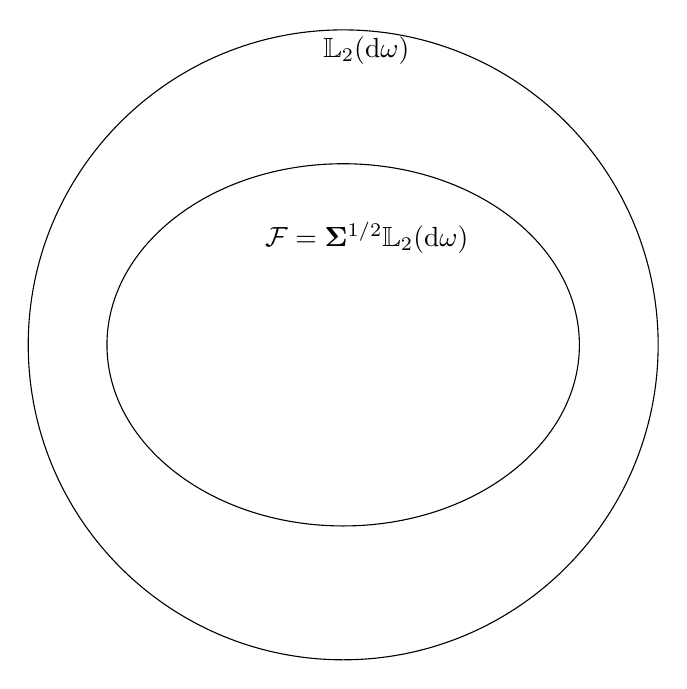
\begin{tikzpicture}[]
\coordinate (A) at (1.4,1,0);
\coordinate (B) at (6.7,1,0);
\coordinate (B2) at (4.1,1,0);
\coordinate (C) at (6.7,-3,0);
\coordinate (D) at (8,-0.3,0);
\coordinate (E) at (8,-1.7,0);

\coordinate (F) at (4,-1,0);


\draw (0,1) circle (4cm);

%\draw (0,1) ellipse (3.5cm and 3.3cm);

%\draw (0,1) ellipse (3cm and 2.6cm);

\draw (0,1) ellipse (3cm and 2.3cm);


% \draw (8,1) circle (1.2cm);

% \draw (8,-3) circle (1.2cm);
% \draw[fill={rgb:red,1;white,5}] (0,0,0) -- (2,0,0) -- (2,2,0) -- (0,2,0) -- cycle;
% \draw[fill={rgb:blue,1;white,5}, opacity=0.5] (0,0,0) -- (2.2,1,0) -- (2.2,3,0) -- (0,2,0) -- cycle;

% \node[canvas is plane={O(0,2,0)x(0,1,0)y(1,2,0)}] at (0.9,-0.9) {\includegraphics[width=2.4cm, height=2.4cm]{fig/principalangles/signal_eigreconstruction_modes}};

% \node[canvas is plane={O(0,2,0)x(0,1,0)y(2.2/2.41,2+1/2.41,0)}] at (0.8,-0.6,0.1) {\includegraphics[width=2.4cm, height=2.7cm]{fig/principalangles/signal_reconstruction_principle_2}};

\begin{scope}
 %  \draw (12.2,1.8,0) node[above left = 0.5mm] {$\mathbb{B}_{\langle .,. \rangle_{\mathcal{F}}} = \bm{\Sigma}^{1/2}\mathbb{B}_{\langle .,. \rangle_{\mathrm{d}\omega}}$};
	% \draw (1.8,1.8,0) node[above left = 0.5mm] {$\mathbb{B}_{\langle .,. \rangle_{\mathrm{d}\omega}}$};
  \draw (1,4.4,0) node[above left = 0.5mm] {$\mathbb{L}_{2}(\mathrm{d}\omega$)};

 %  \draw (1.2,3.5,0) node[above left = 0.5mm] {$\bm{\Sigma}^{1/2}\mathbb{L}_{2}(\mathrm{d}\omega$)};
 %  \draw (0.5,-2.2,0) node[above left = 0.5mm] {$\mathcal{F}$};

 %  \draw (1.4,2.7,0) node[above left = 0.5mm] {$\bm{\Sigma}^{1/2+\color{red}r\color{black}}\mathbb{L}_{2}(\mathrm{d}\omega$)};

	\draw (1.75,2,0) node[above left = 0.5mm] {$\mathcal{F} = \bm{\Sigma}^{1/2}\mathbb{L}_{2}(\mathrm{d}\omega$)};

  % \draw [->] (A) --(B2) node[above] {$\bm{\Sigma}^{1/2}$} -- (B) ;
  % \draw [->] (A) -- (F) node[above] {$\bm{\Sigma}$} -- (C) ;
  % \draw [->] (D) -- (E) ;
\end{scope}
% \begin{scope}[canvas is yz plane at x=1.25]
% \draw[fill={rgb:blue,1;white,5}] (0,0) -- (2,0) -- (2,2) -- (0,2) -- cycle;
% \end{scope}
\end{tikzpicture}
%}}
    \caption{The RKHS $\F$ is an ellipsoid in $\mathbb{L}_{2}(\mathrm{d}\omega)$. \label{fig:rkhs_is_ellipsoid}}
\end{figure}


The compactness assumption in Theorem~\ref{thm:Mercer_for_compact} excludes some classic RKHSs: the RKHSs corresponding to the Gaussian kernel or the Laplace kernels on $\mathbb{R}^{d}$...
Hence the need to an extension of this result to non-compact spaces.

In \cite{Sun05}, the author extended Theorem~\ref{thm:Mercer_for_compact} to $\mathcal{X} = \cup_{i \in \mathbb{N}} \mathcal{X}_{i}$, with the $\mathcal{X}_{i}$s compact and $\mathrm{d}\omega(\mathcal{X}_{i})<\infty$. One can also extend Mercer's theorem under a \textit{compact embedding} assumption \citep{StSc12}: the RKHS $\mathcal{F}$ associated to $k$ is said to be compactly embedded in $\mathbb{L}_{2}(\mathrm{d}\omega)$ if the application
\begin{align*}
  I_{\mathcal{F}}: \mathcal{F}&\longrightarrow \mathbb{L}_{2}(\mathrm{d}\omega) \\
  f &\longmapsto f
\end{align*}
is compact.
A sufficient condition for this assumption is the integrability of the diagonal (Lemma 2.3, \citep{StSc12}), that is,
\begin{equation}
\int_{\mathcal{X}} k(x,x) \mathrm{d}\omega(x) < \infty.
\end{equation}
Note that this condition is not necessary (Example 2.9, \citep{StSc12}). Now, under the compact embedding assumption, the pointwise convergence of the Mercer decomposition to the kernel $k$ is equivalent to the injectivity of the embedding $I_{\mathcal{F}}$ (Theorem 3.1, \citep{StSc12}).
% This condition is satisfied whenever $k$ is bounded and $\mathrm{d}\omega(\mathcal{X}) < \infty$.
% \begin{theorem}[Theorem 3.1, \cite{StSc12}]
% Let $\mathcal{X}$ be a measurable space and $\mathrm{d}\omega$ a measure on $\mathcal{X}$. Let $k$ be a measurable positive kernel on $\mathcal{X}$ with an RKHS $\mathcal{F}$. Assume that $\mathcal{F}$ is compactly embedded in $\mathbb{L}_{2}(\mathrm{d}\omega)$. Define the integral operator $\bm{\Sigma}$:
% \begin{equation}
% \bm{\Sigma} f(x) = \int\limits_{\mathcal{X}} k(x,y)f(y) \mathrm{d}\omega(y).
% \end{equation}
% Then, there exists an orthonormal basis $(e_{n})_{n \in \mathbb{N}}$ of $\mathbb{L}_{2}(\mathrm{d}\omega)$ consisting of eigenfunctions of $\bm{\Sigma}$ and the corresponding eigenvalues are non negatives. The eigenfunctions corresponding to non-vanishing eigenvalues can be taken as continuous functions and the kernel $k$ writes
% \begin{equation}
% k(x,y) = \sum\limits_{n \in \mathbb{N}} \sigma_{n} e_{n}(x)e_{n}(y),
% \end{equation}
% where the convergence is absolute and uniform.
% \end{theorem}
% % \subsection{The results}

\subsection{Further examples of kernels}
\label{subsec:kernel_examples}


\subsubsection{Dot product kernels on hypersphers}

Let $\mathcal{X}$ bet the $d$-dimensional hypersphere $\mathbb{S}^{d} \subset \mathbb{R}^{d+1}$ equipped with the ... associated to the uniform measure $\mathrm{d}\omega$. Let $(a_{m})_{ m \in \mathbb{N}}$ be a sequence of non-negative real numbers, and consider the kernel $k$ defined on $\X$ by
\begin{equation}
k(x,y) = \sum\limits_{m \in \mathbb{N}} a_m L_{m}^{d}(x^{\Tran}y),
\end{equation}
where the $(L_{m}^{d})_{m \in \mathbb{N}}$ are the associated Legendre polynomials of order $d$.

For every, ..., define $Y_{n,j}^{d}$ the $n$-spherical harmonic of dimension $d$ and ...

By Funk-Hecke equation
\begin{equation}
L_{m}^{d}(x^{\Tran}y) = \frac{...}{N(d,m)} \sum\limits_{j =1}^{N(d,m)} Y_{m,j}^{d}(x)Y_{m,j}^{d}(y),
\end{equation}

\subsection{The integration error}
\label{subsec:int_error}
When the integrand $f$ belongs to $\mathcal{F}$, the integration error reads \citep{SmGrSoSc07}
\begin{align}
\label{eq:integral_bound_mean_element}
  \bigg|\int_{\mathcal{X}} f(x)g(x)\mathrm{d}\omega(x) - \sum\limits_{j \in [N]} w_{j}f(x_{j}) \bigg|
  %
  & = \bigg|\langle f, \mu_{g} - \sum\limits_{j \in [N]} w_{j} k(x_{j},.) \rangle_{\mathcal{F}} \bigg|\nonumber\\
  & \leq \|f\|_{\mathcal{F}} \, \Big\|\mu_{g} - \sum\limits_{j \in [N]} w_{j} k(x_{j},.)\Big\|_{\mathcal{F}}\,,
\end{align}
where
\begin{equation}
\mu_{g} = \int_{\mathcal{X}} k(x,.) g(x) \mathrm{d}\omega(x)
\end{equation}
 is the so-called \emph{mean element} \citep{DiPi14,MuFuSrSc17} of the measure $g \mathrm{d}\omega$ or the \emph{embedding} of $g$. \eqref{eq:integral_bound_mean_element} entails that the approximation error of the embedding $\mu_{g}$ by the kernel translates $\sum_{n \in [N]} w_{n}k(x_{n},.)$ in the RKHS norm gives an upper bound on the integration error of the quadrature $(\bm{x}, \bm{w})$, independently of the integrand $f$. It actually is the worst case integration error in the unit ball of $\F$,
\begin{equation}\label{eq:wce_kquadrature}
\sup\limits_{\substack{f \in \mathcal{F}\\ \|f\|_{\mathcal{F}} \leq 1}} \bigg|\int_{\mathcal{X}} f(x)g(x)\mathrm{d}\omega(x) - \sum\limits_{j \in [N]} w_{j}f(x_{j}) \bigg| = \|\mu_{g} - \sum\limits_{n \in [N]}w_{n} k(x_{n},.) \|_{\mathcal{F}}.
\end{equation}




The characterization~\eqref{eq:wce_kquadrature}, of the worst case integration error, motivates the use of a kernel in the evaluation of a quadrature. This idea can be tracked to Hickernell \citep{Hic96,Hic98} who introduced reproducing kernels to the QMC community. Indeed, \cite{Hic96} derived a tractable formula for the worst-case integration error of a quasi-Monte Carlo rule ($\X=[0,1]^{d}$, $g$ is the constant function that take the value $1$ and $w_{n}= 1/N$)

\begin{equation}\label{eq:wce_qmc}
 \sup\limits_{\substack{f \in \mathcal{F}\\ \|f\|_{\mathcal{F}} \leq 1}} \bigg|\int_{[0,1]^{d}} f(x)\mathrm{d}x - \frac{1}{N}\sum\limits_{n \in [N]} f(x_{n}) \bigg|^{2}.
\end{equation}
In particular, he proved that \eqref{eq:wce_qmc} is equal to 
\begin{equation}\label{eq:wce_qmc_2}
 \int_{[0,1]^{d}}\int_{[0,1]^{d}} k(x,y) \mathrm{d}x \mathrm{d}y - \frac{2}{N}\sum\limits_{n \in [N]} \int_{[0,1]^{d}} k(x_{n},y) \mathrm{d} y + \frac{1}{N^2}\sum\limits_{n,n'=1}^{N}k(x_{n},x_{n'}).
\end{equation}

The generalization of \eqref{eq:wce_qmc_2} can be easily derived using properties of reproducing kernels:
\begin{align}
\|\mu_{g} - \sum\limits_{n \in [N]}w_{n} k(x_{n},.) \|_{\mathcal{F}}^{2} & = \|\mu_{g}\|_{\mathcal{F}}^{2} - 2 \langle \mu_{g}, \sum\limits_{n \in [N]}w_{n} k(x_{n},.)  \rangle_{\mathcal{F}} + \|\sum\limits_{n \in [N]}w_{n} k(x_{n},.)\|_{\mathcal{F}}^{2}\\
& = \|\mu_{g}\|_{\mathcal{F}}^{2} - 2 \sum\limits_{n \in [N]} w_{n} \mu_{g}(x_{n}) + \sum\limits_{n,n'=1}^{N}w_{n}k(x_{n},x_{n'})w_{n'}\\
& \label{eq:wce_kq}= \|\mu_{g}\|_{\mathcal{F}}^{2} - 2 \bm{w}^{\Tran} \mu_{g}(\bm{x}) + \bm{w}^{\Tran} \bm{K}(\bm{x})\bm{w},
\end{align}

where $\bm{K}(\bm{x}) = (k(x_{n},x_{n'}))_{(n,n') \in [N] \times [N]} \in \mathbb{R}^{N \times N}$ and $\mu_{g}(\bm{x}) = (\mu_{g}(x_{n}))_{n \in [N]} \in \mathbb{R}^{N}$.


We can check that \eqref{eq:wce_qmc_2} is a consequence of \eqref{eq:wce_kq}, by taking $\mathcal{X} = [0,1]^{d}$, $w_{n}=1/N$, $g=1$ and $\mathrm{d}\omega$ is the uniform measure on $\X$ and observing that

\begin{align}
\|\mu_{g}\|_{\mathcal{F}}^{2} & = \langle \bm{\Sigma} g,\bm{\Sigma} g \rangle_{\mathcal{F}}\\
& = \langle g, \bm{\Sigma} g \rangle_{\mathrm{d}\omega}\\
& = \int_{\mathcal{X}} g(x) \int_{\mathcal{X}} k(x,y) g(y)\mathrm{d}\omega(y) \mathrm{d}\omega(x)\\
& = \int_{\mathcal{X}} \int_{\mathcal{X}} k(x,y) g(x) g(y)\mathrm{d}\omega(y) \mathrm{d}\omega(x),
\end{align}

and that

\begin{equation}
\bm{w}^{\Tran} \mu_{g}(\bm{x}) = \sum\limits_{n \in [N]} w_{n}\mu_{g}(x_{n}) = \sum\limits_{n \in [N]} w_{n}\int_{\mathcal{X}}g(y)k(x_{n},y) \mathrm{d}\omega(y).
\end{equation}



\begin{figure}[]
    \centering
\includegraphics[width= 0.28\textwidth]{img/mean_element/Sobolev/mean_element_cos_ko_1.pdf}~\includegraphics[width= 0.28\textwidth]{img/mean_element/Sobolev/mean_element_saw_ko_1.pdf}~\includegraphics[width= 0.28\textwidth]{img/mean_element/Sobolev/mean_element_step_ko_1.pdf}\\
\caption{$\mu_{g}$ in the periodic Sobolev space for three different $g$.
\label{fig:mean_element}}
\end{figure}


In other words, quasi-Monte Carlo rules fit within the kernel framework of quadratures. 



% A tight approximation of the mean element by a linear combination of functions $k(x_{j},.)$ thus guarantees low quadrature error.


% \paragraph{Kernel quadrature and QMC}



% We recall in the following the aspects shared between kernel quadrature and quasi-Monte Carlo methods and we show the potential benefits of optimal kernel quadrature rules. 

% \subsection{The link with Bayesian quadrature}
% \label{subsec:bayesian_quadrature}

\subsection{Optimal kernel quadrature}
\label{subsec:okq_analysis_paradigm}

As we have seen in Section~\ref{subsec:int_error}, the worst case integration error for a given quadrature $(\bm{x}, \bm{w})$ writes:
\begin{equation}\label{eq:wce_repeated}
\bigg \|\mu_{g} - \sum\limits_{n \in [N]} w_{n}k(x_{n},.) \bigg\|_{\mathcal{F}}.
\end{equation}
Under the assumption that the configuration  $\bm{x} \subset \mathcal{X}$ is uni-solvent with respect to the kernel $k$, i.e. the matrix $\bm{K}(\bm{x}) = (k(x_{n},x_{n'}))_{n,n' \in [N]}$ is non-singular, there exists a unique vector $\bm{w} \in \mathbb{R}^{N}$ that minimizes~\eqref{eq:wce_repeated}. Indeed, the square of \eqref{eq:wce_repeated} is quadratic on $\bm{w}$ so that the optimization problem
\begin{equation}\label{eq:wce_repeated_optimization}
\min\limits_{\bm{w} \in \mathbb{R}^{N}} \bigg \|\mu_{g} - \sum\limits_{n \in [N]} w_{n}k(x_{n},.) \bigg\|_{\mathcal{F}}^{2}
\end{equation}
have a unique solution $\hat{\bm{w}}(\bm{x}) = \bm{K}(\bm{x})^{-1}\mu_{g}(\bm{x})$. The quadrature $(\bm{x},\hat{\bm{w}}(\bm{x}))$ is called the \emph{optimal kernel quadrature} in $\bm{x}$. 

Now, under the assumption that $\bm{K}(\bm{x})$ is non-singular, the dimension of the subspace $\mathcal{T}(\bm{x}) = \Span (k(x_{n},.))_{n \in [N]}$ is equal to $N$. Define 
\begin{equation}
	\bm{\Phi}:(w_{j})_{j \in [N]} \mapsto \sum_{j \in [N]} w_{j} k(x_{j},.)
\end{equation}
 the reconstruction operator\footnote{The reconstruction operator $\bm{\Phi}$ depends on the nodes $x_{j}$, although our notation doesn't reflect it for simplicity.}. The optimal approximation of $\mu_{g}$ by an element of $\mathcal{T}(\bm{x})$, with respect to the RKHS norm, is $\bm{\Phi}\hat{\bm{w}}$, and the optimal approximation error writes
\begin{equation}
\|\mu_{g} - \bm{\Phi}\hat{\bm{w}}\|^{2}_{\mathcal{F}} =\|\mu_{g} - \bm{\Pi}_{\mathcal{T}(\bm{x})}\mu_{g}\|^{2}_{\mathcal{F}},\label{e:finalTool}
\end{equation}
%  The approximation error writes
% \begin{align}
% \|\mu_{g} - \bm{\Phi}\hat{\bm{w}}\|^{2}_{\mathcal{F}} &= \|\mu_{g} - \bm{\Phi}\bm{K}(\bm{x})^{-1} \mu_{g}(x_{i})_{i \in [N]}\|^{2}_{\mathcal{F}}\\
%  &= \|\mu_{g} - \bm{\Phi}(\bm{\Phi}^{*}\bm{\Phi})^{-1}\bm{\Phi}^{*} \mu_{g} \|^{2}_{\mathcal{F}}\\
% &=\|\mu_{g} - \bm{\Pi}_{\mathcal{T}(\bm{x})}\mu_{g}\|^{2}_{\mathcal{F}},\label{e:finalTool}
% \end{align}
where $\bm{\Pi}_{\mathcal{T}(\bm{x})} = \bm{\Phi}(\bm{\Phi}^{*}\bm{\Phi})^{-1}\bm{\Phi}^{*}$ is the orthogonal projection onto $\mathcal{T}(\bm{x})$ with $\bm{\Phi}^{*}$ the dual\footnote{For $\mu \in \mathcal{F}$,$\bm{\Phi}^{*}\mu = (\mu(x_{j}))_{j \in [N]}$. $\bm{\Phi}^{*}\bm{\Phi}$ is an operator from $\mathbb{R}^{N}$ to $\mathbb{R}^{N}$ that can be identified with $\bm{K}(\bm{x})$.} of $\bm{\Phi}$. $\bm{\Phi}\hat{\bm{w}}$ is the orthogonal projection of $\mu_{g}$ on the subspace $\mathcal{T}(\bm{x})$. Moreover, we can prove easily that $\bm{\Phi}\hat{\bm{w}}$ interpolates $\mu_{g}$ on the nodes $x_{1}, \dots, x_{N}$:
\begin{equation}
\forall n \in [N], \:\bm{\Phi}\hat{\bm{w}}(x_{n}) = \mu_{g}(x_{n}).
\end{equation}
We define the \emph{interpolation error} of $\mu_{g}$:
\begin{equation}
\|\mu_{g}- \Pi_{\mathcal{T}(\bm{x})}\mu_{g}\|_{\mathcal{F}}.
\end{equation}
As we have seen, under the assumption that the matrix $\bm{K}(\bm{x})$ is non-singular, the computation of the weights of the optimal kernel quadrature is a relatively simple task. Yet the task of designing a good configuration $\bm{x}$ is not trivial as we shall see in the next section where we review the main results on the literature about design problems for optimal kernel quadrature.
\subsection{Designs for optimal kernel quadrature}
We review in this section the literature on the design of configurations for optimal kernel quadrature.
\subsubsection{Deterministic configurations}
\cite{Boj81} proved that, for $g=1$, the interpolation of $\mu_{g}$ using the uniform grid over $\X = [0,1]$ has an error in $\mathcal{O}(N^{-2s})$ if $\F$ is the periodic Sobolev space of order $s$, and that any set of nodes leads to that rate at least. A similar rate was proved for $g$ not constant \citep{NoUlWo15} even though it is only asymptotically optimal in that case.
% , is optimal\rb{What do you mean by optimal at this stage?} for the  , with a convergence rate in $\mathcal{O}(N^{-2s})$. If $g$ is not constant, the uniform grid is only optimal for large values of $N$  but the convergence rate remains $\mathcal{O}(N^{-2s})$ \citep{NoUlWo15}.

In the quasi-Monte Carlo (QMC) literature, several designs were investigated for $\X = [0,1]^{d}$, $g = 1$ and $\F$ that may not even be a Hilbert space; see \citep{DiPi10}. In this context, the term \emph{QMC quadrature rule} means a low discrepancy sequence, loosely speaking a ``well-spread" set of nodes, along with uniform weights $w_{i} \equiv 1/N$. If $\F$ is a Korobov space of order $s \geq 1$, the Halton sequence of nodes \citep{Hal64} leads to $\mathcal{E}(\mu_1; \bm{x}, (1/N))^2$ in $\mathcal{O}(\log(N)^{2d} N^{-2})$ and higher-order digital nets converge faster as $\mathcal{O}(\log(N)^{2sd} N^{-2s})$ \citep{DiPi14}[Theorem 5].

These rates are naturally inherited if the uniform weights are replaced by the respective optimal weights $\hat{\bm{w}}$, as observed by \cite{BOGOS2019}. In particular, \cite{BOGOS2019} emphasize that the bound for higher-order digital nets attains the optimal rate in this RKHS.
For optimal kernel quadrature based on Halton sequences, this inheritance argument does not explain the fast $\mathcal{O}(\log(N)^{2sd} N^{-2s})$ rates observed empirically by \cite{Oett17}.

Beside the hypercube, optimal kernel quadrature has been considered on the hypersphere equipped with the uniform measure \citep{EhGrCh19}, or on $\mathbb{R}^{d}$ equipped with the Gaussian measure \citep{KaSa19}. In these works, the design construction is adhoc for the space $\X$ and
%except for the case of the uniform grid in $\X = [0,1]$,
$g$ is usually assumed to be constant. Another approach is offered by optimisation algorithms that we review in Section~\ref{sec:sequential_algos}. Before that, we clarify the subtle difference between optimal kernel quadrature and kernel interpolation.

\subsubsection{Sequential Bayesian quadrature}\label{subsec:bayesian_quadrature}

****

\emph{Bayesian Quadrature} \citep{Lar72} initially considered a fixed set of nodes and put a Gaussian process prior on the integrand $f$. Then, the weights were chosen to minimize the posterior variance of the integral of $f$. If the kernel of the Gaussian process is chosen to be $k$, this amounts to minimizing the RHS of \eqref{eq:integral_bound_mean_element}. The case of the Gaussian reference measure was later investigated in detail \citep{Hag91}, while parametric integrands were considered in \citep{Min00}.

\subsubsection{Ridge leverage score quadrature}
\label{subsec:okq_algebraic_paradigm}
The regularization of the problem~\eqref{eq:wce_repeated_optimization} offers an alternative approach for the design of the configuration $\bm{x}$ as it was shown in \citep{Bac17}.
% A similar problem is the desig alternative approach is the regularization of the problem .... 
This work highlights the fundamental role played by the spectral decomposition of the operator $\bm{\Sigma}$ in designing and analyzing kernel quadrature rules.
In fact, the author proposed to sample the nodes $(x_j)$ i.i.d. from some proposal distribution $q$, and then take the vector of weights $\bm{w}$ to be the vector $\bm{w}_{\lambda}$ that solve the optimization problem
\begin{equation}\label{eq:reg_kernel_opt_problem}
\min\limits_{w \in \mathbb{R}^{N}} \Big\| \mu_{g} - \sum\limits_{j \in [N]} \frac{w_{j}}{q(x_{j})^{1/2}} k(x_{j},.) \Big\|_{\mathcal{F}}^{2} + \lambda N \|w\|_{2}^{2},
\end{equation}
for some regularization parameter $\lambda>0$. 

% The idea of the author was to make use of the spectral decomposition of the integral operator $\bm{\Sigma}: \mathbb{L}_{2}(\mathrm{d}\omega) \rightarrow \mathbb{L}_{2}(\mathrm{d}\omega)$ defined by
% \begin{equation}
% \bm{\Sigma} f (\cdot) = \int_{\mathcal{X}} k(\cdot,y)f(y) \mathrm{d}\omega(y), \quad f \in \mathbb{L}_{2}(\mathrm{d}\omega),
% \end{equation}
% in the design and the analysis of the worst integration error of the quadrature. 

% In fact, 

% Finally, we note that Proposition~\ref{p:bach} highlights the fundamental role played by the spectral decomposition of the operator $\bm{\Sigma}$ in designing and analyzing kernel quadrature rules.
 

% In order to understand the importance of the spectral decomposition of $\bm{\Sigma}$ in the design of the quadrature, 

Within this analysis, any proposal distribution $q$, with $q>0$, could be used to sample $N$ i.i.d. nodes that constitutes the design $\bm{x}$: this follows from the following result.

\begin{proposition}[Proposition 1 in \cite{Bac17}]
\label{p:bach_general_proposal}
Let $\delta \in ]0,1]$, and denote
\begin{equation}
d_{\max}(q,\lambda) = \sup\limits_{x \in \X} \frac{1}{q(x)} \langle k(x,.), (\bm{\Sigma}+\lambda \mathbb{I}_{\mathbb{L}_{2}(\mathrm{d}\omega)})^{-1}k(x,.) \rangle_{\mathbb{L}_{2}(\mathrm{d}\omega)}.
\end{equation}
Assume that $N \geq 5 d_{\max}(q,\lambda) \log(16 d_{\max}(q,\lambda) / \delta)$, then
\begin{equation}
\Prb \bigg( \sup\limits_{\|g\|_{\mathrm{d}\omega} \leq 1} \inf\limits_{\|\bm{w}\|^{2}\leq \frac{4}{N}} \Big\| \mu_{g} - \sum\limits_{j \in [N]} \frac{w_{j}}{q_\lambda(x_{j})^{1/2}} k(x_{j},.)\Big\|_{\mathcal{F}}^{2} \leq 4\lambda \bigg) \geq 1- \delta .
\end{equation}
\end{proposition}



In other words, Proposition~\ref{p:bach_general_proposal} gives a uniform  control on the approximation error $\mu_{g}$ by the subspace spanned by the $k(x_{j},.)$ for $g$ belonging to the unit ball of $\mathbb{L}_{2}(\mathrm{d}\omega)$, where the $(x_{j})$ are sampled i.i.d. from $q$. The required number of nodes is equal to $\mathcal{O}(d_{\max}(q,\lambda)\log d_{\max}(q,\lambda))$ for a given approximation error $\lambda$. This bound is relevant if an upper bound of the \emph{maximal ridge leverage score} $d_{\max}(q,\lambda)$ is known. This is possible in some cases; yet in general this quantity is hard to control. Nevertheless, the author showed that one may use a specific choice of $q$, namely the ridge leverage score distribution $q_{\lambda}^{*}$ defined as

\begin{equation}
q_{\lambda}^*(x) \propto \langle k(x,.), \bm{\Sigma}^{-1/2}(\bm{\Sigma}+ \lambda \mathbb{I}_{\mathbb{L}_{2}(\mathrm{d}\omega)})^{-1}\bm{\Sigma}^{-1/2} k(x,.) \rangle_{\mathbb{L}_{2}(\mathrm{d}\omega)} = \sum\limits_{m \in \mathbb{N}^{*}} \frac{\sigma_{m}}{\sigma_{m}+\lambda} e_{m}(x)^{2}.
\label{e:proposalBach}
\end{equation}
Indeed, for this specific choice of $q$
\begin{align}
d_{\max}(q_{\lambda}^{*},\lambda) & = \int_{\X}\langle k(x,.), \bm{\Sigma}^{-1/2}(\bm{\Sigma}+ \lambda \mathbb{I}_{\mathbb{L}_{2}(\mathrm{d}\omega)})^{-1}\bm{\Sigma}^{-1/2} k(x,.) \rangle_{\mathbb{L}_{2}(\mathrm{d}\omega)} \mathrm{d}\omega(x) \nonumber \\
& = \sum\limits_{m \in \mathbb{N}^{*}} \frac{\sigma_{m}}{\sigma_{m}+\lambda} \nonumber\\
& =\Tr \bm{\Sigma}(\bm{\Sigma} + \lambda \bm{I})^{-1}  ,
\end{align}
and the quantity 
\begin{equation}
d_\lambda = \Tr \bm{\Sigma}(\bm{\Sigma} + \lambda \bm{I})^{-1},
\end{equation}
is called the \emph{effective degree of freedom}. This quantity is more amenable to analysis as it depends only on $\lambda$ and on the eigenvalues of $\bm{\Sigma}$.
An instantiation of Proposition~\ref{p:bach_general_proposal} using the ridge leverage score distribution $q_{\lambda}^{*}$ yields the following result.

\begin{proposition}[Proposition 2 in \cite{Bac17}]
\label{p:bach}
Let $\delta \in ]0,1]$. Assume that $N \geq 5 d_\lambda \log(16 d_\lambda / \delta)$, then
\begin{equation}
\Prb \bigg( \sup\limits_{\|g\|_{\mathrm{d}\omega} \leq 1} \inf\limits_{\|\bm{w}\|^{2}\leq \frac{4}{N}} \Big\| \mu_{g} - \sum\limits_{j \in [N]} \frac{w_{j}}{q_\lambda(x_{j})^{1/2}} k(x_{j},.)\Big\|_{\mathcal{F}}^{2} \leq 4\lambda \bigg) \geq 1- \delta .
\end{equation}
\end{proposition}

Now, for fixed $\lambda$, the approximation error in Proposition~\ref{p:bach} does not go to zero when $N$ increases. One theoretical  workaround is to make $\lambda=\lambda(N)$ decrease with $N$. However, the coupling of $N$ and $\lambda$ through $d_\lambda$ makes it very intricate to derive a convergence rate from Proposition~\ref{p:bach}.
Moreover, the optimal density $q_{\lambda}^*$ is in general only available as the limit \eqref{e:proposalBach}, which makes sampling and evaluation difficult. 


\section{Projection DPP for optimal kernel quadrature}\label{sec:pDPP_OKQ}
% \subsubsection{The proposed algorithm}
In this section, we give our first contribution of this chapter \citep{BeBaCh19}. We propose to study optimal kernel quadrature based on nodes that follows the distribution of a projection DPP. We follow in the footsteps of \cite{Bac17}, as reviewed in Section~\ref{subsec:okq_algebraic_paradigm}, but with two main differences:
\begin{itemize}
\item we study the un-regularized optimization problem \eqref{eq:wce_repeated_optimization},
\item we use a projection DPP rather than independent sampling to obtain the nodes.
\end{itemize}

In a nutshell, we consider nodes $(x_{j})_{j \in [N]}$ that are drawn from the projection DPP with reference measure $\mathrm{d}\omega$ and marginal kernel
\begin{equation}
  \KDPP(x,y) = \sum\limits_{n \in [N]} e_{n}(x)e_{n}(y),
  \label{e:kernel}
\end{equation}
where we recall that $(e_{n})_{n \in \mathbb{N}^{*}}$ is an o.n.b of $\mathbb{L}_{2}(\mathrm{d}\omega)$ that diagonalizes $\bm{\Sigma}$; see Section~\ref{subsec:mercer}. As seen in Chapter~\ref{chapter:dpp}, this boils down to sample a random configuration $\bm{x}$ in $\mathcal{X}^{N}$ from the probability distribution

\begin{equation}\label{eq:pdpp_definition}
\frac{1}{N!} \Det(\KDPP(x_{i},x_{j})_{i,j \in [N]}) \prod_{i \in [N]} \mathrm{d}\omega(x_{i}).
\end{equation}



As we shall see, among many possible choices of kernels, the one defined in~\eqref{e:kernel} stands out for several reasons: i) it is intuitive and comes with a theoretical analysis, ii)
it defines a random configuration such that the un-regularized optimization problem~\eqref{eq:wce_repeated_optimization} admits a unique solution with probability one, iii) it is amenable to exact sampling in many settings.

We explain more in detail these three reasons in the following and we start by the first one. This projection DPP defines a uni-solvent configuration $\bm{x}$ with respect to the kernel $k$: the subspace $\mathcal{T}(\bm{x}) = \Span (k(x_{n},.))_{n \in [N]}$ is $N$-dimensional a.s., or equivalently, the matrix $\bm{K}(\bm{x})$ is invertible a.s. This is a consequence of the following result.



\begin{proposition}\label{prop:K_N_non_singular}
Assume that the matrix
$\bm{E}(\bm{x}) = (e_{i}(x_{j}))_{ i,j \in [N]}$ is invertible, then $\bm{K}(\bm{x})$ is invertible.
\end{proposition}
The proof of Proposition~\ref{prop:K_N_non_singular} is given in Section~\ref{app:K_N_non_singular}.
Since the pdf \eqref{eq:pdpp_definition} of the projection DPP with kernel \eqref{e:kernel} is proportional to $\Det^2\bm{E}(\bm{x})$, the following corollary immediately follows.


\begin{corollary}
  Let $\bm{x} = \{x_{1}, \dots , x_{N}\}$ be a projection DPP with reference measure $\mathrm{d}\omega$ and kernel $\KDPP$ defined in \eqref{e:kernel}. Then $\bm{K}(\bm{x})$ is a.s. invertible, so that \eqref{eq:wce_repeated_optimization} has unique solution $\hat{\bm{w}} = \bm{K}(\bm{x})^{-1}\mu_{g}(x_{j})_{j \in [N]}$ a.s.
\label{c:regularization}
\end{corollary}


% We will give a proof of the previous claim, but first observe that the uni-solvency of some configuration $\bm{x}$ with respect to $k$ guarantees the uniqueness of the solution of the optimization problem 
% \begin{equation}\label{eq:unreg_opt_problem}
% \min\limits_{w \in \mathbb{R}^{N}} \| \mu_{g} - \bm{\Phi} \bm{w} \|_{\mathcal{F}}^{2},
% %\quad \text{ where } \quad
% %\bm{\Phi}:(w_{j})_{j \in [N]} \mapsto \sum\limits_{j \in [N]} w_{j} k(x_{j},.).
% \end{equation}

% where
% \begin{equation}
% 	\bm{\Phi}:(w_{j})_{j \in [N]} \mapsto \sum_{j \in [N]} w_{j} k(x_{j},.)
% \end{equation}
%  is the reconstruction operator\footnote{The reconstruction operator $\bm{\Phi}$ depends on the nodes $x_{j}$, although our notation doesn't reflect it for simplicity.}.
%  In fact, \begin{equation}
% \| \mu_{g} - \bm{\Phi} \bm{w} \|_{\mathcal{F}}^{2} = \|\mu_{g}\|_{\mathcal{F}}^{2} - 2 \bm{w}^{\Tran} \mu_{g}(x_{j})_{j \in [N]} + \bm{w}^{\Tran} \bm{K}(\bm{x}) \bm{w},
% \label{e:quadratic}
% \end{equation}
% where $\bm{K}(\bm{x}) = (k(x_{i},x_{j}))_{i,j \in [N]}$. The right-hand side of \eqref{e:quadratic} is quadratic in $\bm{w}$, so that the optimization problem \eqref{eq:unreg_opt_problem}
% % \begin{equation}
% %   \label{e:optimization}
% % \min\limits_{w \in \mathbb{R}^{N}} \| \mu_{g} - \bm{\Phi} \bm{w} \|_{\mathcal{F}}^{2}
% % \end{equation}
% admits a unique solution $\hat{\bm{w}}$ if and only if $\bm{K}(\bm{x})$ is invertible. This latter is equivalent to $\mathcal{T}(\bm{x}) = \Span (k(x_{n},.))_{n \in [N]}$ being an $N$-dimensional subspace. In this case, the solution is given by $\hat{\bm{w}} = \bm{K}(\bm{x})^{-1}\mu_{g}(x_{j})_{j \in [N]}$. A sufficient condition for the invertibility of $\bm{K}(\bm{x})$ is given in the following proposition.
%%% PROPOSITION
% Let $\{x_{1}, \dots, x_{N}\} \in \mathcal{X}^{N}$ be such that



 As we have seen in Section~\ref{subsec:okq_analysis_paradigm}, under the assumption that $\bm{K}(\bm{x})$ is non singular the optimal approximation of $\mu_{g}$ by an element of $\mathcal{T}(\bm{x})$, with respect to the RKHS norm, is $\bm{\Phi}\hat{\bm{w}}$. The optimal approximation error then writes
\begin{equation}
\|\mu_{g} - \bm{\Phi}\hat{\bm{w}}\|^{2}_{\mathcal{F}} =\|\mu_{g} - \bm{\Pi}_{\mathcal{T}(\bm{x})}\mu_{g}\|^{2}_{\mathcal{F}},\label{e:finalTool}
\end{equation}
%  The approximation error writes
% \begin{align}
% \|\mu_{g} - \bm{\Phi}\hat{\bm{w}}\|^{2}_{\mathcal{F}} &= \|\mu_{g} - \bm{\Phi}\bm{K}(\bm{x})^{-1} \mu_{g}(x_{i})_{i \in [N]}\|^{2}_{\mathcal{F}}\\
%  &= \|\mu_{g} - \bm{\Phi}(\bm{\Phi}^{*}\bm{\Phi})^{-1}\bm{\Phi}^{*} \mu_{g} \|^{2}_{\mathcal{F}}\\
% &=\|\mu_{g} - \bm{\Pi}_{\mathcal{T}(\bm{x})}\mu_{g}\|^{2}_{\mathcal{F}},\label{e:finalTool}
% \end{align}
where $\bm{\Pi}_{\mathcal{T}(\bm{x})} = \bm{\Phi}(\bm{\Phi}^{*}\bm{\Phi})^{-1}\bm{\Phi}^{*}$ is the orthogonal projection onto $\mathcal{T}(\bm{x})$ with $\bm{\Phi}^{*}$ the dual\footnote{For $\mu \in \mathcal{F}$,$\bm{\Phi}^{*}\mu = (\mu(x_{j}))_{j \in [N]}$. $\bm{\Phi}^{*}\bm{\Phi}$ is an operator from $\mathbb{R}^{N}$ to $\mathbb{R}^{N}$ that can be identified with $\bm{K}(\bm{x})$.} of $\bm{\Phi}$: $\bm{\Phi}\hat{\bm{w}}$ is the orthogonal projection of $\mu_{g}$ on the subspace $\mathcal{T}(\bm{x})$. 


% Moreover, we can prove easily that $\bm{\Phi}\hat{\bm{w}}$ interpolates $\mu_{g}$ on the nodes $x_{1}, \dots, x_{N}$:
% \begin{equation}
% \forall n \in [N], \:\bm{\Phi}\hat{\bm{w}}(x_{n}) = \mu_{g}(x_{n}).
% \end{equation}
Now, the second reason to introduce the projection DPP associated to the the kernel~\eqref{e:kernel} is the possibility of the theoretical analysis of the expected value of 
 \begin{equation}
 \|\mu_{g} - \bm{\Pi}_{\mathcal{T}(\bm{x})} \mu_{g}\|_{\mathcal{F}}^{2}.
 \end{equation}



We explain this point more in detail after presenting our theoretical guarantees in the following section. The details of the proofs are given in Section~\ref{s:proofs}.

% To see this, we give the main results of this chapter, before 
% This is achieved by considering the following upper bound for the interpolation error.

% From the proof of Proposition~\ref{prop:K_N_non_singular}, it seems that the first eigenfunctions that are involved into the definition of the kernel~\eqref{e:kernel}
%  can be replaced by any set of $N$ eigenfunctions of $\bm{\Sigma}$. Yet, we will see that this specific choice of \eqref{e:kernel} allows a 


% %\subsubsection{The theoretical guarantees}
% Now consider $\bm{x} = \{x_{1}, \dots, x_{N} \} \subset \mathcal{X}$. The weights $\bm{w}$ are obtained by solving the optimization problem
%  In Section~\ref{subsec:unreg_opt_problem} we prove that \eqref{eq:unreg_opt_problem} almost surely has a unique solution $\hat{\bm{w}}$ and state our main result, an upper bound on the expected approximation error $\|\mu_{g} - \bm{\Phi}\hat{\bm{w}}\|^{2}_{\mathcal{F}}$ under the proposed Projection DPP. 


 %%%%%%%%
\subsection{The main results}
\label{subsec:unreg_opt_problem}
% Besides the uni-solvency property of the projection DPP defined in the beginning of this section, this choice of marginal kernel is amenable to theoretical analysis.



% Assuming that nodes $(x_{j})_{j \in [N]}$ are known, we first need to solve the optimization problem \eqref{eq:unreg_opt_problem} that relates to problem~\eqref{eq:reg_kernel_opt_problem} without regularization ($\lambda = 0$).
% %
% Let $\bm{x} = (x_{1}, \dots, x_{N}) \in \mathcal{X}^{N}$, then
% using the fact that $\langle \mu, k(x_{i},.) \rangle_{\mathcal{F}} = \mu(x_{i})$:
% \begin{align}
% \| \mu - \bm{\Phi} \bm{w} \|_{\mathcal{F}}^{2} & = \|\mu\|_{\mathcal{F}}^{2} - 2 \sum\limits_{i \in [N]} w_{i} \mu(x_{i}) + \sum\limits_{1\leq i,j \leq N}w_{i}w_{j}k(x_{i},x_{j})\\
% &= \|\mu\|_{\mathcal{F}}^{2} - 2 \bm{w}^{\Tran} \mu(x_{i})_{i \in [N]} + \bm{w}^{\Tran} \bm{K} \bm{w}.
% \end{align}

%%%
In the section, we present the theoretical analysis of $\|\mu_{g} - \bm{\Pi}_{\mathcal{T}(\bm{x})} \mu_{g}\|_{\mathcal{F}}^{2}$ under the projection DPP $(\KDPP, \mathrm{d}\omega)$, where $\KDPP$ is defined in \eqref{e:kernel}. We start with a result that we obtained in \citep*{BeBaCh19}, which quantifies the expected interpolation error in terms of the spectrum of the integration operator $\bm{\Sigma}$.

% We present in this section,in th the  result and its consequences in this section.
%%% THEOREM
\begin{theorem}\label{thm:main_theorem}
Let $\bm{x} = \{x_{1}, \dots , x_{N}\}$ be a random set that follows the distribution of the projection DPP $(\KDPP,\mathrm{d}\omega )$. Let $g \in \mathbb{L}_{2}(\mathrm{d}\omega)$ such that $\|g\|_{\mathrm{d}\omega} \leq 1$. Then, 
\begin{equation}\label{eq:main_result_first}
\EX_{\DPP} \|\mu_{g} - \bm{\Pi}_{\mathcal{T}(\bm{x})} \mu_{g}\|_{\mathcal{F}}^{2}  \leq
2\sigma_{N+1} +2\|g\|_{\mathrm{d}\omega,1}^{2}\left(   N r_{N} + \sum\limits_{\ell =2}^{N} \frac{\sigma_{1}}{\ell!^{2}}\left(\frac{Nr_{N}}{\sigma_{1}}\right)^{\ell} \right),
\end{equation}
where $\displaystyle \|g\|_{\mathrm{d}\omega,1} = \sum\limits_{n \in [N]} |\langle e_{n},g \rangle_{d\omega}|$ and $r_{N} = \sum\limits_{m \geq N+1} \sigma_{m}$. Moreover, 
\begin{equation}\label{eq:main_result_sup_first}
\EX_{\DPP} \sup\limits_{\|g\|_{\mathrm{d}\omega} \leq 1} \|\mu_{g} - \bm{\Pi}_{\mathcal{T}(\bm{x})} \mu_{g}\|_{\mathcal{F}}^{2}  \leq
2\sigma_{N+1} +2N\left(   N r_{N} + \sum\limits_{\ell =2}^{N} \frac{\sigma_{1}}{\ell!^{2}}\left(\frac{Nr_{N}}{\sigma_{1}}\right)^{\ell} \right).
\end{equation}
%with
%\begin{equation}
%	\label{eq:def_rN}
%	r_{N} = \sum\limits_{m \geq N+1} \sigma_{m}.
%\end{equation}
\end{theorem}
%%%


Since the publication of \citep{BeBaCh19}, we obtained a refinement of Theorem~\ref{thm:main_theorem} that we give in the following.


\begin{theorem}\label{thm:main_theorem_improved}
Let $\bm{x} = \{x_{1}, \dots , x_{N}\}$ be a random set that follows the distribution of the projection DPP $(\mathrm{d}\omega, \KDPP )$. Let $g \in \mathbb{L}_{2}(\mathrm{d}\omega)$ such that $\|g\|_{\mathrm{d}\omega} \leq 1$. Then, 
\begin{equation}\label{eq:main_result}
\EX_{\DPP} \|\mu_{g} - \bm{\Pi}_{\mathcal{T}(\bm{x})} \mu_{g}\|_{\mathcal{F}}^{2}  \leq
2\sigma_{N+1} +2\|g\|_{\mathrm{d}\omega,1}^{2} N r_{N} ,
\end{equation}
where $\displaystyle \|g\|_{\mathrm{d}\omega,1} = \sum\limits_{n \in [N]} |\langle e_{n},g \rangle_{d\omega}|$ and $r_{N} = \sum\limits_{m \geq N+1} \sigma_{m}$. Moreover, 
\begin{equation}\label{eq:main_result_sup}
\EX_{\DPP} \sup\limits_{\|g\|_{\mathrm{d}\omega} \leq 1} \|\mu_{g} - \bm{\Pi}_{\mathcal{T}(\bm{x})} \mu_{g}\|_{\mathcal{F}}^{2}  \leq
2\sigma_{N+1} +2N^{2} r_{N}.
\end{equation}
%with
%\begin{equation}
%	\label{eq:def_rN}
%	r_{N} = \sum\limits_{m \geq N+1} \sigma_{m}.
%\end{equation}
\end{theorem}

Let us comment on the upper bounds of Theorem~\ref{thm:main_theorem_improved}. The first term in the upper bounds \eqref{eq:main_result} and \eqref{eq:main_result_sup} scales as $\sigma_{N+1}$. As we shall in Section ??, $\sigma_{N+1}$ is the lower bound of interpolation in a sense that will be defined. The second terms in the upper bounds \eqref{eq:main_result} and \eqref{eq:main_result_sup} stem from our proof technique. Indeed, the constant $\|g\|_{\mathrm{d}\omega,1}$ in $\eqref{eq:main_result}$ is the $\ell_1$ norm of the coefficients of the projection of $g$ onto $\Span(e_{n})_{n \in [N]}$ in $\mathbb{L}_{2}(\mathrm{d}\omega)$. For example, for $g = e_{n}$, $\|g\|_{\mathrm{d}\omega,1} = 1$ if $n \in [N]$ and $\|g\|_{\mathrm{d}\omega,1} = 0$ if $n \geq N+1$. In the worst case, $\|g\|_{\mathrm{d}\omega,1} \leq \sqrt{N} \|g\|_{\mathrm{d}\omega} \leq \sqrt{N}$.
% \begin{equation}\label{eq:l1_worst_case}
% .\leq \sqrt{N} \sqrt{\sum\limits_{n \in [N]} \langle g, e_{n} \rangle_{\mathrm{d}\omega}^{2}}
% \end{equation}
Thus, we can obtain a uniform bound for $\|g\|_{\mathrm{d}\omega}\leq 1$ but with a supplementary factor $N$. Now, if $\sum\limits_{m \in \mathbb{N}^{*}} |\langle g,e_{m} \rangle_{\mathrm{d}\omega}| < +\infty$ for a particular $g \in \mathbb{L}_{2}(\mathrm{d}\omega)$, the r.h.s. of \eqref{eq:main_result} is $\mathcal{O}(Nr_{N})$ because $\sigma_{N+1} \leq Nr_{N}$. Similarly, the upper bound in \eqref{eq:main_result_sup} is dominated by $\mathcal{O}(N^{2}r_{N})$.

Both these bounds converge to $0$ if the convergence of $(\sigma_{n})$ to $0$ is fast enough. For example, if $\sigma_{m} = m^{-2s}$, $\mathcal{O}(r_{N}) = N^{1-2s}$ thus $\mathcal{O}(Nr_{N}) = N^{2-2s}$ and $\mathcal{O}(N^{2}r_{N}) = N^{3-2s}$; and convergence is guaranteed if $s >1$ or if $s>3/2$ respectively. Another example is given by $\sigma_{m} = \beta \alpha^{m}$ with $0 < \alpha < 1$ and $\beta >0$ then $Nr_{N} = N\frac{\beta}{1-\alpha}\alpha^{N+1}=  o(1)$ and $N^{2}r_{N} = N^{2}\frac{\beta}{1-\alpha}\alpha^{N+1}=  o(1)$ for all values of $\alpha$ and $\beta$.



% Since, , the uppers bounds are dominated respectively by these upper bounds are carried by  then the right-hand side of \eqref{eq:main_result} is $N r_{N} + o(N r_{N})$. 
% take $\mathcal{X} = [0,1]$, $\mathrm{d}\omega$ the uniform measure on $\mathcal{X}$, and $\mathcal{F}$ the $s$-Sobolev space, then $\sigma_{m} = m^{-2s}$ \cite{BeTh11}. Now, if $s > 1$, the expected worst case quadrature error is bounded by $Nr_{N} = \mathcal{O}(N^{2-2s}) = o(1)$.


% $\mathrm{d}\omega_{\nu}(x) = (2\pi\nu^{2})^{-1/2}e^{-\frac{1}{2\nu^{2}}x^{2}}$
% $k_{\gamma}(x,y) = \exp[-(x-y)^{2}/2\gamma^{2}]$


% \footnote{$\alpha_{\nu,\gamma} = \frac{1}{1+\frac{1}{2}\rho^{2}+\sqrt{\rho^{2}+\frac{1}{4}\rho^{4}}}$ and $\beta_{\nu,\gamma} = \sqrt{\frac{2}{1+\frac{1}{\rho}+\sqrt{1+2\frac{1}{\rho}}}}$, where $\rho = \frac{\gamma}{\nu}$ \cite{RaWi06} .}
We have assumed that $\mathcal{F}$ is dense in $\mathbb{L}_{2}(\mathrm{d}\omega)$ but Theorem~\ref{thm:main_theorem_improved} is valid also when $\mathcal{F}$ is finite-dimensional. In this case, denote $N_{0} = \dim \mathcal{F}$. Then, for $n > N_{0}$, $\sigma_{n} = 0$ and $r_{N_{0}} = 0$, so that \eqref{eq:main_result} implies
\begin{equation}
  \| \mu_{g} - \bm{\Pi}_{\mathcal{T}(\bm{x})}\mu_{g}\|_{\mathcal{F}}= 0 \:\: \text{a.s.}
\end{equation}
when $N= N_0$.
This compares favourably with the quadrature based on herding with uniform weights that comes with a rate in $\mathcal{O}(\frac{1}{N})$  \citep{ChWeSm10,BaLaOb12}. 


% \paragraph{The Gaussian kernel}
% Let,
% \begin{equation}
% k(x,y) = e^{-\frac{(x-y)^{2}}{2a^{2}}},
% \end{equation}
% with
% \begin{equation}
% \mathrm{d}\omega(x) = \frac{1}{\sqrt 2 \sigma}e^{-\frac{x^{2}}{\sigma^2}},
% \end{equation}
% then \cite{Ras03}
% \begin{equation}
% \sigma_{m} = A B^{m},
% \end{equation}
% and
% \begin{equation}
% e_{m} = e^{-(c-a)x^{2}}H_{m}(\sqrt{2c}x).
% \end{equation}


% Of course, the results in Theorem~\ref{thm:main_theorem_refined} are stronger compared to the ones in Theorem~\ref{thm:main_theorem}. Yet, we think that the proof of Theorem~\ref{thm:main_theorem_refined} will become clearer if we recall the proof of Theorem~\ref{thm:main_theorem} and the intuitions behind. 


In comparison with \cite{Bac17}, we emphasize that the dependence of our bound on the eigenvalues of the kernel $k$, via $r_{N}$, is explicit. This is in contrast with Proposition~\ref{p:bach} that depends on the eigenvalues of $\bm{\Sigma}$ through the degree of freedom $d_{\lambda}$ so that the necessary number of samples $N$ diverges when $\lambda \rightarrow 0$. On the contrary, our quadrature requires a finite number of points for $\lambda =0$. 

% It would be interesting to extend the analysis of our quadrature in the regime $\lambda >0$.


Another advantage of DPPs is that they can be sampled exactly. Because of the orthonormality of $(\psi_n)$, one can write the chain rule for \eqref{eq:pdpp_definition}; see \citep{HoKrPeVi06}. Sampling each conditional in turn, using e.g. rejection sampling \citep{RoCa04}, then yields an exact sampling algorithm. Rejection sampling aside, the cost of this algorithm is cubic in $N$ without further assumptions on the kernel. The main limitation is the availability of good proposals for the successive rejection sampling routines.

%Simplifying assumptions can take many forms. 
Theorem~\ref{thm:main_theorem_improved} gives a slightly sharper bound than Theorem~\ref{thm:main_theorem}, since if $Nr_{N} = o(1)$, then the right-hand side of \eqref{eq:main_result_first} is $N r_{N} + o(N r_{N})$. The proof of Theorem~\ref{thm:main_theorem_improved} follows the same steps as the proof of Theorem~\ref{thm:main_theorem}. We give the proofs of the two results simultaneously in the following section and we highlight the difference between the two in the end of the section.


% We give the proofs of Theorem~\ref{thm:main_theorem} and Theorem~\ref{thm:main_theorem_improved} in the following section. 

% shares 
% The following section contains the sketch of the proof of this result. 

% Again, the proof is based on the quantification of principal angles between subspaces. We recall this notion in the following section.

 % weak version of our results, while Section~\ref{subsec:dpp_quadrature_error_strong} contains the sketch of the proof of the strong version of our results.

% \subsection{Principal angles between subspaces in a Hilbert space}
% \label{subsec:principalangles}
% We recall in this section the definition of principal angles between subspaces in Hilbert spaces and we present a result that will be used later in the proofs. 

% %%% PROPOSITION

% We refer to \cite{GoVa12} for the proof when $\mathcal{H}$ is finite-dimensional. We give a proof in the general case in ??; see also \cite{DaKa70}.
%%%%%%%%%%%%%%
% \begin{proof}
% Assume that $\mathcal{P}_{1} \cap \mathcal{P}_{2} \neq \{\bm{0} \}$ and put $p = \dim \mathcal{P}_{1} \cap \mathcal{P}_{2}$. Let $(\bm{v}^{1}_{i})_{i \in [p]} = (\bm{v}^{2}_{i})_{i \in [p]}$ an orthonormal basis of $\mathcal{P}_{1} \cap \mathcal{P}_{2}$, and denote for $i \in [p], \: \theta_{i} = 0$. If $p = N$, $\mathcal{P}_{1} = \mathcal{P}_{2} = \mathcal{P}_{1} \cap \mathcal{P}_{2}$ and $\theta_{1} = \dots = \theta_{N} = 0$. If not, the subspace $\mathcal{P}_{1} \cap \mathcal{P}_{2}$ is strictly included in $\mathcal{P}_{1}$ and $\mathcal{P}_{2}$ such that the subspaces $\mathcal{P}_{1} \cap (\mathcal{P}_{1} \cap \mathcal{P}_{2})^{\perp}$ and $\mathcal{P}_{2} \cap (\mathcal{P}_{1} \cap \mathcal{P}_{2})^{\perp}$ are non-trivial. Now, let
% \begin{equation}
% \mathcal{P}_{1}^{0} = \mathcal{P}_{1} \cap (\mathcal{P}_{1} \cap \mathcal{P}_{2})^{\perp},
% \end{equation}
% and
% \begin{equation}
% \mathcal{P}_{2}^{0} = \mathcal{P}_{2} \cap (\mathcal{P}_{1} \cap \mathcal{P}_{2})^{\perp}.
% \end{equation}
%
% Define $(\bm{v}^{1}_{p +1}, \bm{v}^{2}_{p +1}) \in \mathcal{P}_{1}^{0} \times \mathcal{P}_{2}^{0}$ such that
% \begin{equation}
% \langle \bm{v}^{1}_{p +1}, \bm{v}^{2}_{p +1} \rangle_{\mathcal{H}} = \max\limits_{\substack{\bm{v}^{1} \in \mathcal{P}_{1}^{0},\bm{v}^{2} \in \mathcal{P}_{2}^{0}\\ \|\bm{v}^{1}\| = 1, \|\bm{v}^{2}\| = 1}} \langle \bm{v}^{1}, \bm{v}^{2} \rangle_{\mathcal{H}},
% \end{equation}
% and put $\theta_{p+1} \in [0, \frac{\pi}{2}]$ such that $\cos \theta_{p+1} = \langle \bm{v}^{1}_{p +1}, \bm{v}^{2}_{p +1} \rangle_{\mathcal{H}}$. Now if $p+1 < N$, define for $\ell \in [N-p]$ recursively the subspaces
% \begin{equation}
% \mathcal{P}_{1}^{\ell} = \mathcal{P}_{1}^{\ell-1} \cap \bm{v}^{1 \perp}_{p+\ell},
% \end{equation}
% and
% \begin{equation}
% \mathcal{P}_{2}^{\ell} = \mathcal{P}_{2}^{\ell-1} \cap \bm{v}^{2 \perp}_{p+\ell},
% \end{equation}
% along with  $(\bm{v}^{1}_{p+\ell+1},\bm{v}^{2}_{p+\ell+1}) \in \mathcal{P}_{1}^{\ell} \times \mathcal{P}_{2}^{\ell}$ such that
% \begin{equation}
% \langle \bm{v}^{1}_{p +\ell+1}, \bm{v}^{2}_{p +\ell+1} \rangle_{\mathcal{H}} = \max\limits_{\substack{\bm{v}^{1} \in \mathcal{P}_{1}^{\ell},\bm{v}^{2} \in \mathcal{P}_{2}^{\ell}\\ \|\bm{v}^{1}\| = 1, \|\bm{v}^{2}\| = 1}} \langle \bm{u}, \bm{v} \rangle_{\mathcal{H}} ,
% \end{equation}
% and let $\theta_{p +\ell+1} \in [0, \frac{\pi}{2}]$ such that $\langle \bm{v}^{1}_{p +\ell+1}, \bm{v}^{2}_{p +\ell+1} \rangle_{\mathcal{H}} = \cos \theta_{p +\ell+1}$. By construction $(\bm{v}^{1}_{\ell})_{\ell \in [N]}$ is an orthonormal basis of $\mathcal{P}_{1}$ and $(\bm{v}^{2}_{\ell})_{\ell \in [N]}$ is an orthonormal basis of $\mathcal{P}_{2}$ such that
% \begin{equation}
% \forall i \in [N], \: \langle \bm{v}^{1}_{i}, \bm{v}^{2}_{i} \rangle_{\mathcal{H}} = \cos \theta_{i}.
% \end{equation}
% \end{proof}

%%%%%%%%%%%%
% The following result shows that the principal angles are somewhat independent of the choice of orthonormal bases. It can be found in \cite{BjGo73,MiBe92} for the finite dimensional case. We give here the proof for the general case, for the sake of completeness.
% \begin{proposition}\label{prop:cos_det_relationship}
% Let $(\bm{w}^{1}_{i})_{i \in [N]}$ be any orthonormal basis of $\mathcal{P}_{1}$ and $(\bm{w}^{2}_{i})_{i \in [N]}$ be any orthonormal basis of $\mathcal{P}_{2}$, and let $\bm{W} = (\langle \bm{w}^{1}_{i},\bm{w}^{2}_{j} \rangle_{\mathcal{H}})_{1\leq i,j \leq N}$ and $\bm{G} = \bm{W}\bm{W}^{\Tran}$. Then
% the eigenvalues of $\bm{G}$ are the $\cos^{2} \theta_{i}(\mathcal{P}_{1},\mathcal{P}_{2})$. In particular, $\Det^{2} \bm{W} = \Det \bm{G} =  \prod\limits_{i \in [N]} \cos^{2} \theta_{i}(\mathcal{P}_{1},\mathcal{P}_{2})$.
% \end{proposition}
%%%%%%%%%%%%


% \pc{ Ici il faudra en dire un peu plus quand même... ce n'est pas si facile à voir.}
%  Another interesting property of the kernel $\tilde{k}$ is that the interpolation errors of $(e_{n}^{\tilde{\mathcal{F}}})_{n \in [N]^{0}}$ are equal.
% \begin{proposition}\label{prop:equality_of_interpolation_errors}
% Let $\tilde{k}$ as defined in \eqref{eq:tilde_k_kernel_definition}, and $\mathcal{F}$ the corresponding RKHS. Then,
% \begin{equation}
% \forall n \in [N]^{0}, \: \|\bm{\Pi}_{\tilde{\mathcal{T}}_{N}(\bm{x})^{\perp}} e_{n}^{\tilde{\mathcal{F}}}\|_{\tilde{\mathcal{F}}}^{2} = \|\bm{\Pi}_{\tilde{\mathcal{T}}_{N}(\bm{x})^{\perp}} e_{0}^{\tilde{\mathcal{F}}}\|_{\tilde{\mathcal{F}}}^{2}.
% \end{equation}
% \end{proposition}


\subsection{Bounding the interpolation error under the projection DPP}
\label{subsec:dpp_quadrature_error_weak}
In this section, we give the skeleton of the proofs of Theorem~\ref{thm:main_theorem} and Theorem~\ref{thm:main_theorem_refined}. The details of the proofs are deferred to Section~\ref{s:proofs}.

The starting point of the analysis is the observation that the interpolation error is the RKHS norm of the residual $\mu_{g} - \bm{\Pi}_{\mathcal{T}(\bm{x})} \mu_{g}$. Since the subspace $\mathcal{T}(\bm{x})$ can be arbitrary, as $\bm{x}$ spans the set of uni-solvent of $\X$ of cardinality $N$, it is hard to reckon how large the corresponding residual can be. For this reason, we consider the principal subspace $\mathcal{E}_N^{\mathcal{F}} = \Span(e_{n}^{\mathcal{F}})_{n \in [N]}$ and the corresponding \emph{filtering error} $\|\mu_{g} - \bm{\Pi}_{\mathcal{E}_{N}^{\mathcal{F}}} \mu_{g}\|_{\mathcal{F}}$. The filtering error is easier to quantify because we can prove easily that

\begin{equation}
\|\mu_{g} - \bm{\Pi}_{\mathcal{E}_{N}^{\mathcal{F}}} \mu_{g}\|_{\mathcal{F}}^{2} = \sum\limits_{m \geq N+1} \langle \mu_{g},e_{m}^{\mathcal{F}} \rangle_{\mathcal{F}}^{2} = \sum\limits_{m \geq N+1} \sigma_{m} \langle g,e_{m} \rangle_{\mathrm{d}\omega}^{2}.
\end{equation}
In particular, when $\|g\|_{\mathrm{d}\omega} \leq 1$, $\|\mu_{g} - \bm{\Pi}_{\mathcal{E}_{N}^{\mathcal{F}}} \mu_{g}\|_{\mathcal{F}}^{2} \leq \sigma_{N+1}$, with equality when $g = e_{n+1}$. Moreover, if the two subspaces $\mathcal{E}_{N}^{\mathcal{F}}$ and $\mathcal{T}(\bm{x})$ are close to each other in some sense, we expect to have $\|\mu_{g} - \bm{\Pi}_{\mathcal{T}(\bm{x})} \mu_{g}\|_{\mathcal{F}}^{2}$ close to  $\sigma_{N+1}$ when $\|g\|_{\mathrm{d}\omega} \leq 1$. As a first step, we have the following lemma that gives an upper bound of $\|\mu_{g} - \bm{\Pi}_{\mathcal{T}(\bm{x})}\mu_{g}\|^{2}_{\mathcal{F}}$ using the $\|\mu_{e_{n}^{\F}} - \bm{\Pi}_{\mathcal{T}(\bm{x})} \mu_{e_{n}^{\F}}\|_{\mathcal{F}}^{2}$.

%$\| \bm{\Sigma}^{-1/2} \mu_{g} \|_{\mathcal{F}} \leq 1$

\begin{lemma}\label{lemma:approximation_error_spectral_bound}
Assume that $\|g\|_{\mathrm{d}\omega} \leq 1$ then 
\begin{equation}
	\|\mu_{g} - \bm{\Pi}_{\mathcal{T}(\bm{x})}\mu_{g}\|^{2}_{\mathcal{F}} \leq 2 \bigg( \sigma_{N+1} + \|g\|_{\mathrm{d}\omega,1}^2  \max\limits_{ n \in [N]} \|\mu_{e_{n}^{\F}} - \bm{\Pi}_{\mathcal{T}(\bm{x})} \mu_{e_{n}^{\F}}\|_{\mathcal{F}}^{2} \bigg) .
\label{e:boundingOrthogonalProjection}
\end{equation}
% with $\displaystyle c(g) = \sum\limits_{n \in [N]} |\langle \bm{\Sigma}^{-1/2} \mu_{g}, e_{n}^{\mathcal{F}} \rangle_{\mathcal{F}}| = \sum\limits_{n \in [N]} |\langle g, e_{n} \rangle_{\mathrm{d}\omega}|$.
\end{lemma}
The term $2 \sigma_{N+1}$ converges to $0$ when $N$ goes to $+\infty$ and we shall see later that it scales as a specific lower bound. Now it remains to upper bound the $\|\mu_{e_{n}^{\F}} - \bm{\Pi}_{\mathcal{T}(\bm{x})} \mu_{e_{n}^{\F}}\|_{\mathcal{F}}^{2}$  for $n \in [N]$ that also have the following expression
% In other words, the upper bound of $\|\mu_{g} - \bm{\Pi}_{\mathcal{T}(\bm{x})}\mu_{g}\|^{2}_{\mathcal{F}}$ decomposes on two terms: $\sigma_{N+1}$ that represents the interpolation error  and  $\|\mu_{e_{n}^{\F}} - \bm{\Pi}_{\mathcal{T}(\bm{x})} \mu_{e_{n}^{\F}}\|_{\mathcal{F}}^{2}$ 
% We give the proof of this lemma later. For now, we observe that for every $n$
\begin{equation}\label{eq:interpolation_at_eigenfunctions_equivalent_expression}
 \|\mu_{e_{n}^{\F}} - \bm{\Pi}_{\mathcal{T}(\bm{x})} \mu_{e_{n}^{\F}}\|_{\mathcal{F}}^{2} =  \sigma_{n} \|e_{n}^{\F} - \bm{\Pi}_{\mathcal{T}(\bm{x})} e_{n}^{\F}\|_{\mathcal{F}}^{2}.
\end{equation}
% We argue that if $\bm{x}$ follows the distribution of the mentioned projection DPP, we can quantify the proximity between these two subspaces.
% , where   is the ....   analysis of the  error  that the interpolation error $\|\mu_{g} - \Pi_{\mathcal{T}(\bm{x})} \mu_{g}\|^{2}_{\mathcal{F}}$ is the residual of 
%  % the skeleton of the proof of Theorem~\ref{thm:main_theorem}, referring to the appendices for technical details.
%   The proof is in two steps. First, we give an upper bound for the approximation error $\|\mu_{g} - \bm{\Phi}\hat{\bm{w}}\|^{2}_{\mathcal{F}}$ that involves the maximal principal angle between the functional subspaces of $\mathcal{F}$
% $$\mathcal{E}_N^{\mathcal{F}} = \Span(e_{n}^{\mathcal{F}})_{n \in [N]} \quad\text{ and }\quad \mathcal{T}(\bm{x}) = \Span(k(x_{j},.))_{j \in [N]}.$$
% The second step consists in developing the expectation of the bound under the projection DPP in a similar fashion as in Chapter ??: projection DPPs allow closed form expressions for the expectation of some trigonometric functions of the principal angles.
% This quantification is achieved by the principal angles between subspaces 
% As for now, we recall some properties of the principal angles between subspaces of a Hilbert space and we give the corresponding instantiation of these results when the Hilbert space is $\F$.
% \rb{Make this an assumption using begin/end{assumption}, and comment on it, saying what it means and that others used the same.}

\begin{figure}[]
\centering

\makeatletter
\tikzoption{canvas is plane}[]{\@setOxy#1}
\def\@setOxy O(#1,#2,#3)x(#4,#5,#6)y(#7,#8,#9)%
  {\def\tikz@plane@origin{\pgfpointxyz{#1}{#2}{#3}}%
   \def\tikz@plane@x{\pgfpointxyz{#4}{#5}{#6}}%
   \def\tikz@plane@y{\pgfpointxyz{#7}{#8}{#9}}%
   \tikz@canvas@is@plane
  }
\makeatother 
%\resizebox{4.5cm}{!}{
% \begin{tikzpicture}[y={(-1cm,0.5cm)},x={(1cm,0.5cm)}, z={(0cm,1cm)}]
\begin{tikzpicture}[y={(-1cm,0.5cm)},x={(1cm,0.5cm)}, z={(0cm,1cm)}]
\coordinate (A) at (0,0,0);
\coordinate (B) at (2,0,0);
\coordinate (C) at (1.1*1.8,1.1*1.5,0);
%1.8/2.34,2+1.5/2.34,0
\draw[fill={rgb:red,1;white,5}] (0,0,0) -- (2,0,0) -- (2,2,0) -- (0,2,0) -- cycle;
\draw[fill={rgb:blue,1;white,5}, opacity=0.5] (0,0,0) -- (1.1*1.8,1.1*1.5,0) -- (1.1*1.8,2+1.1*1.5,0) -- (0,2,0) -- cycle;
%\node[transform shape] at (0,0) (ImageA)  {\includegraphics[width=3cm]{fig/signal_reconstruction_principle_2.pdf}};

%\node[canvas is plane={O(0,0,0)x(2.2/2.41,1/2.41,0)y(2.2/2.41,3/2.41,0)}] at (1.1,1.1) {\includegraphics[width=4cm]{fig/signal_reconstruction_principle_2.pdf}};
\node[canvas is plane={O(0,2,0)x(0,1,0)y(1,2,0)}] at (0.9,-0.9) {\includegraphics[width=2.4cm, height=2.4cm]{img/principalangles/signal_eigreconstruction_modes.pdf}};

\node[canvas is plane={O(0,2,0)x(0,1,0)y(1.8/2.34,2+1.5/2.34,0)}] at (0.65,-0.35,0.1) {\includegraphics[width=2.4cm, height=2.7cm]{img/principalangles/signal_reconstruction_principle_2.pdf}};

\begin{scope}
	\draw (0,-1.3,0) node[above left = 0.5mm] {$\theta_{N}(\tilde{\mathcal{T}}(\bm{x}),\mathcal{E}_{N}^{\tilde{\mathcal{F}}})$};
	\draw (2.2,-0.8,0) node[below ] {$\mathcal{E}_{N}^{\tilde{\mathcal{F}}} = \Span (e_{j}^{\tilde{\mathcal{F}}})_{j \in [N]}$};
	\draw (-0,6,0) node[below right=0.5mm] {$\tilde{\mathcal{T}}(\bm{x}) = \Span \tilde{k}(x_{i},.)_{i \in [N]}$};
    \clip (C) -- (A) -- (B) -- cycle;
    \draw[-] circle[at=(A),radius=4mm];
  
\end{scope}
% \begin{scope}[canvas is yz plane at x=1.25]
% \draw[fill={rgb:blue,1;white,5}] (0,0) -- (2,0) -- (2,2) -- (0,2) -- cycle;
% \end{scope}
\end{tikzpicture}

%}
 \caption{Illustration of the largest principal angle between the subspaces $\mathcal{T}(\bm{x})$ and $\mathcal{E}_{N}^{\mathcal{F}}$ in the case of the periodic Sobolev space of order 1.  \label{fig:func_principal_angles}}
\end{figure}


To upper bound the right-hand side of \eqref{eq:interpolation_at_eigenfunctions_equivalent_expression}, we note that $\sigma_{n} \|e_{n}^{\F} - \bm{\Pi}_{\mathcal{T}(\bm{x})} e_{n}^{\F}\|_{\mathcal{F}}^{2}$ is the product of two terms: $\sigma_{n}$ is a decreasing function of $n$ while $\|e_{n}^{\F} - \bm{\Pi}_{\mathcal{T}(\bm{x})} e_{n}^{\F}\|_{\mathcal{F}}^{2}$ is the interpolation error of the eigenfunction $e_{n}^{\mathcal{F}}$, measured in the $\|.\|_{\mathcal{F}}$ norm.
We can bound the latter interpolation error uniformly in $n\in [N]$ using the largest principal angle between $\mathcal{T}(\bm{x})$ and $\mathcal{E}^{\mathcal{F}}_{N} = \Span(e_{n}^{\mathcal{F}})_{ n \in [N]}$; see Section?? in Chapter~\ref{chapter:cssp} for details on principal angles between subspaces. 
% \begin{theorem}\label{prop:cos_between_subspaces}
% Let $\mathcal{H}$ be a Hilbert space. Let $\mathcal{P}_{1}$ and $\mathcal{P}_{2}$ be two finite-dimensional subspaces of $\mathcal{H}$ with $N = \dim \mathcal{P}_{1} = \dim \mathcal{P}_{2}$. Denote $\bm{\Pi}_{\mathcal{P}_{1}}$ and $\bm{\Pi}_{\mathcal{P}_{2}}$ the orthogonal projections of $\mathcal{H}$ onto these two subspaces. There exist two orthonormal bases for $\mathcal{P}_{1}$ and $\mathcal{P}_{2}$ denoted $(\bm{v}_{i}^{1})_{i \in [N]}$ and $(\bm{v}_{i}^{2})_{i \in [N]}$, and a set of angles $\theta_{i}(\mathcal{P}_{1},\mathcal{P}_{2}) \in [0,\frac{\pi}{2}]$ such that
% \begin{equation}
% \cos \theta_{N}(\mathcal{P}_{1},\mathcal{P}_{2}) \leq \dots \leq \cos \theta_{1}(\mathcal{P}_{1},\mathcal{P}_{2}) ,
% \end{equation}
% %%%%%%%%%%%
% and for $i \in [1,...,N]$
% \begin{equation}
% \langle \bm{v}_{i}^{1}, \bm{v}_{i}^{2} \rangle_{\mathcal{H}} = \cos \theta_{i}(\mathcal{P}_{1},\mathcal{P}_{2}),
% \end{equation}
% and
% \begin{equation}\label{eq:principal_vectors_projection_relationship}
%  \bm{\Pi}_{\mathcal{P}_{1}}\bm{v}_{i}^{2} = \cos \theta_{i}(\mathcal{P}_{1},\mathcal{P}_{2}) \bm{v}_{i}^{1},
% \end{equation}
% and
% \begin{equation}
%  \bm{\Pi}_{\mathcal{P}_{2}}\bm{v}_{i}^{1} = \cos \theta_{i}(\mathcal{P}_{1},\mathcal{P}_{2}) \bm{v}_{i}^{2}.
% \end{equation}
% In particular
% \begin{equation}\label{eq:costhetaN}
% \cos \theta_{N}(\mathcal{P}_{1},\mathcal{P}_{2}) = \inf\limits_{\bm{v} \in \mathcal{P}_{1},\|\bm{v}\|_{\mathcal{H}} = 1} \|\bm{\Pi}_{\mathcal{P}_{2}}\bm{v}\|_{\mathcal{H}}.
% \end{equation}
% \end{theorem}
In particular, remember that the maximal principal angle is defined through its cosine
\begin{equation}
	\cos^{2} \theta_{N}(\mathcal{T}(\bm{x}),\mathcal{E}^{\mathcal{F}}_{N}) = \inf\limits_{\substack{\bm{u} \in \mathcal{T}(\bm{x}), \bm{v} \in \mathcal{E}^{\mathcal{F}}_{N}\\ \|u\|_{\mathcal{F}} = 1, \|v\|_{\mathcal{F}} = 1}} \langle \bm{u}, \bm{v} \rangle_{\mathcal{F}}.
\end{equation}
We can then define successively the $N-1$ principal angles $\theta_{n}(\mathcal{T}(\bm{x}),\mathcal{E}^{\mathcal{F}}_{N}) \in \left[0, \frac{\pi}{2}\right]$ for $ n\in [N-1]$ between the subspaces $\mathcal{E}^{\mathcal{F}}_{N}$ and $\mathcal{T}(\bm{x})$. These angles quantify the relative position of theses two subspaces. Now, we have the following lemma.






% See Appendix~\ref{subsec:principalangles} for more details about principal angles.
% While principal angles in Euclidean spaces are a well-known notion \cite{GoVa96}, Section 6.4.3., we could not locate their extension to finite-dimensional subspaces of Hilbert spaces in the literature. \ab{This sentence to be discussed}
 % We thus give the necessary details in  .

% In the following, we use the maximal principal angle between the subspaces $\mathcal{E}^{\mathcal{F}}_{N}$ and $\mathcal{T}(\bm{x})$ to bound $\max\limits_{n \in [N]}  \|\bm{\Pi}_{\mathcal{T}(\bm{x})^{\perp}} e_{n}^{\mathcal{F}}\|_{\mathcal{F}}^{2}$.
\begin{lemma}\label{lemma:max_error_cos}
Let $\bm{x} = \{x_{1}, \dots , x_{N}\} \subset \mathcal{X}$ such that $\Det \bm{E}(\bm{x}) \neq 0$. Then
\begin{equation}\label{eq:max_error_as_function_of_cos}
	\max_{ n \in [N]} \|e_{n}^{\F} - \bm{\Pi}_{\mathcal{T}(\bm{x})} e_{n}^{\F}\|_{\mathcal{F}}^{2} \leq \frac{1}{\cos^{2} \theta_{N}(\mathcal{T}(\bm{x}),\mathcal{E}^{\mathcal{F}}_{N})} - 1. 
\end{equation}
In particular
\begin{equation}\label{eq:max_error_as_function_of_cos_prod}
\max_{ n \in [N]} \|e_{n}^{\F} - \bm{\Pi}_{\mathcal{T}(\bm{x})} e_{n}^{\F}\|_{\mathcal{F}}^{2} \leq \prod\limits_{n \in [N]}\frac{1}{\cos^{2} \theta_{n}(\mathcal{T}(\bm{x}),\mathcal{E}^{\mathcal{F}}_{N})} - 1,
\end{equation}
and
\begin{equation}\label{eq:max_error_as_function_of_cos_sum}
\max_{ n \in [N]} \|e_{n}^{\F} - \bm{\Pi}_{\mathcal{T}(\bm{x})} e_{n}^{\F}\|_{\mathcal{F}}^{2} \leq \sum\limits_{n \in [N]}\frac{1}{\cos^{2} \theta_{n}(\mathcal{T}(\bm{x}),\mathcal{E}^{\mathcal{F}}_{N})} - N.
\end{equation}
\end{lemma}





To sum up, we have so far bounded the approximation error by the geometric quantities in the right-hand side of \eqref{eq:max_error_as_function_of_cos_prod} and \eqref{eq:max_error_as_function_of_cos_sum}.
The proof of Theorem~\ref{thm:main_theorem} uses the symmetrization \eqref{eq:max_error_as_function_of_cos_prod}, while
the proof of Theorem~\ref{thm:main_theorem_improved} uses the symmetrization \eqref{eq:max_error_as_function_of_cos_sum}.

As we have seen in Chapter~\ref{chapter:cssp}, projection DPPs shine in taking expectations of such symmetric geometric quantities in finite dimensional vector spaces. We will show in the following that this is also true in RKHSs. Indeed, a simple application of Proposition~\ref{prop:principal_angles_spectral_hilbert_spaces} of Chapter~\ref{chapter:cssp}, in the case $\mathcal{H} = \F$, $\mathcal{P}_{1} = \mathcal{E}_{N}^{\F}$ and $\mathcal{P}_{2} = \mathcal{T}(\bm{x})$ leads to the following result.



\begin{corollary}\label{cor:cos_ratio_det}
Let $\bm{x} =  \{ x_{1}, \dots , x_{N}\} \subset \mathcal{X}$ such that $\Det^{2} \bm{E}(\bm{x}) \neq 0$. Then,
\begin{equation}
\prod\limits_{\ell \in [N]} \frac{1}{\cos^{2} \theta_{\ell} \left(\mathcal{E}^{\mathcal{F}}_{N}, \mathcal{T}(\bm{x}) \right)} = \frac{\Det \bm{K}(\bm{x})}{\Det^{2} \bm{E}^{\mathcal{F}}(\bm{x})},
\end{equation}
and
\begin{equation}
\sum\limits_{\ell \in [N]} \frac{1}{\cos^{2} \theta_{\ell} \bigg(\mathcal{E}^{\mathcal{F}}_{N}, \mathcal{T}(\bm{x}) \bigg)} = \Tr \bigg(\bm{E}^{\mathcal{F}}(\bm{x})^{\Tran^{-1}}  \bm{K}(\bm{x}) \bm{E}^{\mathcal{F}}(\bm{x})^{-1} \bigg).
\end{equation}
\end{corollary}





% \subsubsection{Taking the expectation under the DPP}
% \label{subsec:expectation_under_the_DPP}
Corollary~\ref{cor:cos_ratio_det} allows to obtain tractable formulas, in terms of the eigenvalues of the kernel $k$, of the expectation of the right-hand side of \eqref{eq:max_error_as_function_of_cos_prod} and \eqref{eq:max_error_as_function_of_cos_sum}.
This is achieved in the following two results.
% prove the following two results that   can 

% Now, the upper bound in Lemma~\ref{lemma:max_error_cos} is satisfied whenever $\Det \bm{E}(\bm{x}) \neq 0$. As seen in Corollary~\ref{c:regularization}, this condition is satisfied almost surely when $\bm{x}$ is drawn from the projection DPP $(\mathrm{d}\omega, \KDPP)$. 

The first one concerns the multiplicative symmetrization.
%% Proposition
\begin{proposition}\label{prop:expected_value_of_product_of_cos}
Let $\bm{x} = \{x_{1}, \dots , x_{N}\}$ be a random set that follows the projection DPP $(\mathrm{d}\omega, \KDPP )$. Then,
\begin{equation}\label{eq:expected_value_of_product_of_cos}
\EX_{\DPP} \prod\limits_{n \in [N]} \frac{1}{\cos^{2} \theta_{n}\bigg(\mathcal{T}(\bm{x}), \mathcal{E}^{\mathcal{F}}_{N} \bigg)}   = \sum\limits_{\substack{T \subset \mathbb{N}^{*} \\ |T| = N}} \frac{ \prod\limits_{t \in T}\sigma_{t}}{\prod\limits_{n \in [N]} \sigma_{n}} \:.
\end{equation}
\end{proposition}

The second result concerns the additive symmetrization.

\begin{proposition}\label{prop:ex_dpp_sum_inv_cos}
Let $\bm{x} = \{x_{1}, \dots , x_{N}\}$ be a random set that follows the projection DPP $(\mathrm{d}\omega, \KDPP )$. Then,
\begin{equation}
\EX_{\DPP}  \sum\limits_{\ell \in [N]} \frac{1}{\cos^{2} \theta_{\ell} \bigg(\mathcal{E}^{\mathcal{F}}_{N}, \mathcal{T}(\bm{x}) \bigg)} -N =  \sum\limits_{v \in [N]} \frac{1}{\sigma_{v}} \sum\limits_{w \in \mathbb{N}^{*}\smallsetminus [N]} \sigma_{w}.
\end{equation}
% In particular for the saturated kernel, we have
% \begin{equation}
% \EX_{\DPP}  \sum\limits_{\ell \in [N]} \frac{1}{\cos^{2} \theta_{\ell} \bigg(\mathcal{E}^{\tilde{\mathcal{F}}}_{N}, \tilde{\mathcal{T}}(\bm{x}) \bigg)}  -N =  \frac{N}{\sigma_{1}} \sum\limits_{w \in \mathbb{N}^{*}\smallsetminus [N]} \sigma_{w}.
% \end{equation}
\end{proposition}



% \sum\limits_{n \in [N]}\frac{1}{\sigma_{n}}r_{N} + \dots + \frac{1}{\prod\limits_{n \in [N]} \sigma_{n}} \sum\limits_{\substack{T \subset \mathbb{N}^{*} \smallsetminus [N]\\ |T| = N}}\prod\limits_{t \in T}\sigma_{t}

% & =  \sum\limits_{\substack{T \subset \mathbb{N} \\ |T| = N}} \frac{ \prod\limits_{t \in T}\sigma_{t}}{\prod\limits_{n \in [N]^{0}} \sigma_{n}} -1\\
% &
The bound of Proposition~\ref{prop:expected_value_of_product_of_cos}, once reported in  Lemma~\ref{lemma:max_error_cos} and Lemma~\ref{lemma:approximation_error_spectral_bound}, already yields Theorem~\ref{thm:main_theorem} in the special case where $\sigma_{1} = \dots = \sigma_{N}$. This seems a very restrictive condition, but Proposition~\ref{prop:kernel_perturbation_inequality} below shows that we can always reduce the analysis to that case.
% \subsubsection{An upper bound for $\max\limits_{n \in [N]^{0}} \sigma_{n}\|\Pi_{\mathcal{T}(x)^{\perp}} e_{n}^{\mathcal{F}}\|_{\mathcal{F}}^{2}$}
% In this section, we give a bound of the approximation error $\|f - \bm{\Phi}\hat{\bm{w}}\|_{\mathcal{F}}$ using the maximal principal angle between the subspaces $\mathcal{E} = \Span(e_{m}^{\mathcal{F}})_{m \in [N]}$ and $\mathcal{T}(\bm{x}) =  \Span \bigg( k(x_{i},.) \bigg)_{i \in [N]}$.
In fact, let the kernel $\tilde{k}$ be defined by
\begin{equation}\label{eq:tilde_k_kernel_definition}
\tilde{k}(x,y) = \sum\limits_{n \in [N]} \sigma_{1}e_{n}(x)e_{n}(y) + \sum\limits_{n \geq N+1} \sigma_{n}e_{n}(x)e_{n}(y) = \sum\limits_{n \in \mathbb{N}^{*}} \tilde{\sigma}_{n}e_{n}(x)e_{n}(y),
\end{equation}
and let $\tilde{\mathcal{F}}$ be the corresponding RKHS. Then one has the following inequality.
%% PROPOSITION
\begin{proposition}\label{prop:kernel_perturbation_inequality}
Let $ \tilde{\mathcal{T}}(\bm{x}) = \Span \left( \tilde{k}(x_{j},.) \right)_{j \in [N]}$ and $\bm{\Pi}_{\tilde{\mathcal{T}}(\bm{x})}$ the orthogonal projection onto $\tilde{\mathcal{T}}(\bm{x})$ in $(\tilde{\mathcal{F}}, \langle .,.\rangle_{\tilde{\mathcal{F}}})$. Then,
\begin{equation}\label{eq:kernel_perturbation_inequality}
	\forall n \in [N], \:\: \sigma_{n} \|e_{n}^{\mathcal{F}} - \bm{\Pi}_{\mathcal{T}(\bm{x})} e_{n}^{\mathcal{F}}\|_{\mathcal{F}}^{2} \leq \sigma_{1}   \|e_{n}^{\tilde{\mathcal{F}}} - \bm{\Pi}_{\tilde{\mathcal{T}}(\bm{x})} e_{n}^{\tilde{\mathcal{F}}}\|_{\tilde{\mathcal{F}}}^{2}.
\end{equation}
\end{proposition}
%% END PROPOSITION
Simply put, capping the first eigenvalues of $k$ yields a new kernel $\tilde{k}$ that captures the interaction between the terms $\sigma_{n}$ and $\|e_{n}^{\mathcal{F}} - \bm{\Pi}_{\mathcal{T}(\bm{x})} e_{n}^{\mathcal{F}}\|_{\mathcal{F}}^{2}$, so that we only have to deal with the term $\|e_{n}^{\tilde{\mathcal{F}}} - \bm{\Pi}_{\tilde{\mathcal{T}}(\bm{x})} e_{n}^{\tilde{\mathcal{F}}}\|_{\tilde{\mathcal{F}}}^{2}$.
Combining  Proposition~\ref{prop:expected_value_of_product_of_cos} with Proposition~\ref{prop:kernel_perturbation_inequality} applied to the kernel $\tilde{k}$ yields Theorem~\ref{thm:main_theorem}. 

The same steps are followed to obtain the Theorem~\ref{thm:main_theorem_improved} using Proposition~\ref{prop:ex_dpp_sum_inv_cos}.
 % and Appendix~\ref{app:geometric_intuition} for the geometric intuition behind the proof
% \subsubsection{Bounding the approximation error using principal angles}
% \label{subsec:approximation_error_principal_angle}
% In other words, \eqref{e:finalTool} equates the approximation error to $\|\bm{\Pi}_{\mathcal{T}(\bm{x})^{\perp}}\mu_g\|^{2}_{\mathcal{F}}$, where $\bm{\Pi}_{\mathcal{T}(\bm{x})^{\perp}}$ is the orthogonal projection onto $\mathcal{T}(\bm{x})^{\perp}$.
% % \rb{and maybe give a ref on the definition of the projection, since $\Phi$ is an operator}.
% Now we have the following lemma.
The additive symmetrization gives a neater upper bound compared to the multiplicative symmetrization. Nevertheless the proof of Proposition~\ref{prop:ex_dpp_sum_inv_cos} is more technical.



\section{Numerical simulations}
This section is devoted to numerical simulations that illustrate the main results of Section~\ref{subsec:unreg_opt_problem}.

\subsection{The periodic Sobolev space}\label{s:sobolev_numsim}
Let $\mathrm{d}\omega$ be the uniform measure on $\mathcal{X} = [0,1]$, and let the RKHS kernel be \citep{BeTh11}
\begin{equation}
k_{s}(x,y) = 1+ 2\sum\limits_{m \in \mathbb{N}^{*}} \frac{1}{m^{2s}} \cos(2\pi m(x-y)),
\end{equation}
so that $\mathcal{F}=\mathcal{F}_{s}$ is the periodic Sobolev space of order $s$ on $[0,1]$.

We consider a set of three numerical experiments. In the first one, we consider the approximation of $\mu_{g}$ when $g \equiv 1$ using several quadratures; in the second one, we consider the approximation of $\mu_{g}$ when $g$ is an eigenfunction of $\bm{\Sigma}$ using the optimal kernel quadrature based on the projection DPP; in the third one, we consider the worst interpolation error when $g$ spans the unit ball of $\mathbb{L}_{2}(\mathrm{d}\omega)$. 
\subsubsection{A first experiment}
 We take $g\equiv 1$ so that the mean element $\mu_{g} \equiv 1$. We compare the following algorithms: $(i)$ the quadrature rule DPPKQ we propose in Theorem~\ref{thm:main_theorem} (optimal kernel quadrature based on the projection DPP), $(ii)$ the quadrature rule DPPUQ based on the same projection DPP but with uniform weights $(w_{n} = 1/N)$ \cite{Joh97}, $(iii)$ the kernel quadrature rule \eqref{eq:reg_kernel_opt_problem} of \cite{Bac17}, which we denote LVSQ for \emph{leverage score quadrature}, with regularization parameter $\lambda \in \{0,0.1,0.2\}$ (note that the optimal proposal is $q_{\lambda}^* \equiv 1$), $(iv)$ herding with uniform weights \citep{BaLaOb12,ChWeSm10}, $(v)$ sequential Bayesian quadrature (SBQ) \citep{HuDu12} with regularization to avoid numerical instability, and $(vi)$ optimal kernel quadrature on the uniform grid (UGKQ). We take $N \in [5,50]$. Figure~\ref{fig:pDPP_results_pSobolev_exp_1} shows log-log plots of the worst case quadrature error w.r.t. $N$, averaged over 50 samples for each point, for $s \in \{1,3\}$.


 We observe that the approximation errors of all first four quadratures converge to $0$ with different rates. Both UGKQ and DPPKQ converge to $0$ with a rate of $\mathcal{O}(N^{-2s})$, which indicates that our $\mathcal{O}(N^{2-2s})$ bound in Theorem~\ref{thm:main_theorem} is not tight in the Sobolev case. Meanwhile, the rate of DPPUQ is $\mathcal{O}(N^{-2})$ across the three values of $s$: it does not adapt to the regularity of the integrands. This corresponds to the CLT proven in \cite{Joh97}.
  LVSQ without regularization converges to $0$ slightly slower than $\mathcal{O}(N^{-2s})$. Augmenting $\lambda$ further slows down convergence. Herding converges at an empirical rate of $\mathcal{O}(N^{-2})$, which is faster than the rate $\mathcal{O}(N^{-1})$ predicted by the theoretical analysis in \cite{BaLaOb12,ChWeSm10}. SBQ is the only one that seems to plateau for $s = 3$, although it consistently has the best performance for low $N$.
  % However, we recall that it is the only algorithm here with no theoretical guarantee on its error.
Overall, in the Sobolev case, DPPKQ and UGKQ have the best convergence rate. UGKQ --~known to be optimal in this case \cite{Boj81}~-- has a better constant.



\begin{figure}
\centering
\includegraphics[width=0.45\textwidth]{img/neurips/Sobolev/Sobolev_kernel_order_1_fig_1.pdf}
\includegraphics[width=0.45\textwidth]{img/neurips/Sobolev/Sobolev_kernel_order_3_fig_1.pdf}\\
\caption{Squared approximation error vs. number of nodes $N$ in the case of the periodic Sobolev space for $s = 1$ (left) and $s=3$ (right).
\label{fig:pDPP_results_pSobolev_exp_1}}
\end{figure}

Observe that in this case $g$ is an eigenfunction of $\bm{\Sigma}$ corresponding to the largest eigenvalue that equals $1$. We consider in the next section, the interpolation of $\mu_{g}$ when $g$ is a generic eigenfunction of $\bm{\Sigma}$.

\subsubsection{The reconstruction of the embeddings of eigenfunctions}
We consider $g$ to be an eigenfunction $\bm{\Sigma}$: $g \in \{e_{5},e_{10},e_{14},e_{15},e_{16},e_{17}\}$, so that $\mu_{g} = \bm{\Sigma}g \in \{\sigma_{5}e_{5},\sigma_{10}e_{10},\sigma_{14}e_{14},\sigma_{15}e_{15},\sigma_{16}e_{16},\sigma_{17}e_{17}\}$. We observe the interpolation error under the projection DPP (DPPKQ) for $N \in [5,50]$. Figure~\ref{fig:pDPP_results_pSobolev_exp_2} shows log-log plots of the interpolation error  w.r.t. $N$, averaged over 50 samples for each point, for $s \in \{1,3\}$.


 We observe that for every $g = e_{n}$, the interpolation error goes through two phases: in the first phase ($N < n$) the interpolation error is practically equal to \emph{the initial error} that is $\|\mu_{g}\|_{\mathcal{F}}^{2} = \sigma_{n}$; in the second phase ($N \geq n$) the interpolation error decreases to $0$ at the rate $\mathcal{O}(N^{-2s})$. These observations indicate again that the $\mathcal{O}(N^{2-2s})$ bound in Theorem~\ref{thm:main_theorem} is not tight.
 Moreover, we observe that given two eigenfunctions $e_{n}$ and $e_{n'}$ corresponding to the same eigenvalue, the expected interpolation error is practically the same. This is the case, for instance, of $e_{14}$ and $e_{15}$ or $e_{16}$ and $e_{17}$.
\begin{figure}
\centering
\includegraphics[width=0.45\textwidth]{img/neurips/Sobolev/multig_interpolation_pSobolev_s_1_fig_1.pdf}
\includegraphics[width=0.45\textwidth]{img/neurips/Sobolev/multig_interpolation_pSobolev_s_3_fig_1.pdf}\\
\caption{Squared interpolation error for the embedding of the eigenfunctions vs. number of nodes $N$ in the periodic Sobolev space for $s = 1$ (left) and $s=3$ (right).
\label{fig:pDPP_results_pSobolev_exp_2}}
\end{figure}
\subsubsection{The uniform reconstruction of the embeddings of the element of the unit ball}



In the previous experiments, we investigated empirically the interpolation error $\|\mu_{g}~-~\bm{\Pi}_{\mathcal{T}(\bm{x})}~\mu_{g}\|_{\mathcal{F}}^{2}$ for some functions $g$ in the unit ball of $\mathbb{L}_{2}(\mathrm{d}\omega)$. Remember, that the bound \eqref{eq:main_result_sup} in Theorem~\ref{thm:main_theorem_improved} deals with the worst case interpolation error defined by:
\begin{equation}\label{eq:worst_interpolation_error_supunitball}
\sup\limits_{\|g\|_{\mathrm{d}\omega} \leq 1} \|\mu_{g}-\bm{\Pi}_{\mathcal{T}(\bm{x})} \mu_{g}\|_{\mathcal{F}}^{2}.
\end{equation}

We investigate this quantity by considering the following surrogate:
\begin{equation}\label{eq:surrogate_worst_inerpolation_error}
\sup\limits_{g \in \mathcal{G}_{\Delta} } \|\mu_{g}-\bm{\Pi}_{\mathcal{T}(\bm{x})} \mu_{g}\|_{\mathcal{F}}^{2},
\end{equation}
where $\mathcal{G}_{\Delta} = \{ \frac{1}{\sqrt{\Delta}} \sum\limits_{\delta \in [\Delta]} \epsilon_{\delta} e_{\delta}; \epsilon_{\delta} \in \{-1,1\}\}$ for some $\Delta \in \mathbb{N}^{*}$. The quantity~\eqref{eq:surrogate_worst_inerpolation_error} is an approximation of the worst interpolation error. Indeed, if $g = \sum\limits_{\delta \in [\Delta]} \epsilon_{\delta} e_{\delta}$ for some $(\epsilon_{1}, \dots, \epsilon_{\Delta})$, then $\|g\|_{\mathrm{d}\omega} = 1$.

We compare the following quadratures defined previously: $(i)$ the quadrature rule DPPKQ, $(ii)$ LVSQ with regularization parameter $\lambda = 0$, and $(iii)$ UGKQ. We take $N \in [5,50]$. Figures~\ref{fig:pDPP_results_pSobolev_exp_3_G6} and \ref{fig:pDPP_results_pSobolev_exp_3_G7} show log-log plots of the worst interpolation error, on $\mathcal{G}_{6}$ and $\mathcal{G}_{7}$ respectively, w.r.t. $N$, averaged over 50 samples for each point, for $s \in \{1,3\}$. 



\begin{figure}
\centering
\includegraphics[width=0.45\textwidth]{img/neurips/Sobolev/suponunitball_interpolation_pSobolev_s_1_binarycubeM_64_fig_1.pdf}
\includegraphics[width=0.45\textwidth]{img/neurips/Sobolev/suponunitball_interpolation_pSobolev_s_3_binarycubeM_64_fig_1.pdf}\\
% \includegraphics[width=0.45\textwidth]{img/neurips/Sobolev/suponunitball_interpolation_pSobolev_s_1_binarycubeM_128_fig_1.pdf}
% \includegraphics[width=0.45\textwidth]{img/neurips/Sobolev/suponunitball_interpolation_pSobolev_s_3_binarycubeM_128_fig_1.pdf}\\
\caption{Squared worst interpolation error on $\mathcal{G}_{6}$ error vs. number of nodes $N$ for $s = 1$ (left) and $s=3$ (right).
\label{fig:pDPP_results_pSobolev_exp_3_G6}}
\end{figure}
\begin{figure}
\centering
\includegraphics[width=0.45\textwidth]{img/neurips/Sobolev/suponunitball_interpolation_pSobolev_s_1_binarycubeM_64_fig_1.pdf}
\includegraphics[width=0.45\textwidth]{img/neurips/Sobolev/suponunitball_interpolation_pSobolev_s_3_binarycubeM_64_fig_1.pdf}\\
% \includegraphics[width=0.45\textwidth]{img/neurips/Sobolev/suponunitball_interpolation_pSobolev_s_1_binarycubeM_128_fig_1.pdf}
% \includegraphics[width=0.45\textwidth]{img/neurips/Sobolev/suponunitball_interpolation_pSobolev_s_3_binarycubeM_128_fig_1.pdf}\\
\caption{Squared worst interpolation error on $\mathcal{G}_{7}$ error vs. number of nodes $N$ for $s = 1$ (left) and $s=3$ (right).
\label{fig:pDPP_results_pSobolev_exp_3_G7}}
\end{figure}
% For a given configuration $\bm{x} \subset \X$, the worst interpolation error on $\mathcal{I}$ is defined by
% \begin{equation}
% \sup\limits_{g = \sum\limits_{\delta \in [\Delta]} \epsilon_{\delta} e_{\delta}} \|\mu_{g}-\bm{\Pi}_{\mathcal{T}(\bm{x})} \mu_{g}\|_{\mathcal{F}}^{2}.
% \end{equation}
% We consider the following experience. 
We observe that the worst interpolation errors, of the three quadratures, converge  to $0$. DPPKQ converges at the rate $\mathcal{O}(N^{-2s})$ better than the theoretical rate $\mathcal{O}(N^{3-2s})$ of Theorem~\ref{thm:main_theorem_improved}. UGKQ seems to converge at the rate $\mathcal{O}(N^{-2s})$ with a better constant than DPPKQ. Finally, LVSQ converges at a rate slower than $\mathcal{O}(N^{-2s})$. 

Among the three algorithms, DPPKQ is the only one to have guarantees for the worst interpolation error on the unit ball of $\mathbb{L}_{2}(\mathrm{d}\omega)$~\eqref{eq:worst_interpolation_error_supunitball} although the empirical investigation shows that the rates are pessimistic.

\subsection{The Korobov space}
Now, we consider the Korobov kernel $k_{s,d}$ defined on $[0,1]^{d}$ by
\begin{equation}
\forall x, y \in [0,1]^{d}, \:\:k_{s,d}(x,y) = \prod\limits_{\delta \in [d]} k_{s}(x_{\delta},y_{\delta}).
\end{equation}

% The Mercer decomposition
Remember that the Mercer decomposition of $k_{s,d}$ with respect to the uniform measure $\mathrm{d}\omega(x) = \prod\limits_{\delta \in [d]} \mathrm{d}\omega_{1}(x_{\delta})$, where $\mathrm{d}\omega_{1}$ is the uniform measure on $[0,1]$, writes

\begin{equation}
k_{s,d}(x,y) = \sum\limits_{u \in (\mathbb{N}\smallsetminus \{0\})^{d}} \prod\limits_{\delta \in [d]} \sigma_{\delta}^{1} e_{\delta}^{1}(x_{\delta}) e_{\delta}^{1}(y_{\delta}),
\end{equation}

where the $(\sigma_{m}^{1})$ and the $(e_{m}^{1})$ are respectively the eigenvalues and the eigenfunctions of the kernel $k_{s}$ with respect to the measure $\mathrm{d}\omega_{1}$.


The definition of the DPP kernel $\frak K$ requires to define an order on multi-indices. We choose an order $\prec$ that keeps the eigenvalues of $k_{s,d}$ decreasing:
\begin{equation}
u \prec v \iff  \prod\limits_{\delta \in [d]} \sigma_{u_{\delta}} \leq \prod\limits_{\delta \in [d]} \sigma_{v_{\delta}}.
\end{equation}
% as in the univariate case where $\sigma_{1} \geq \sigma_{2}\geq\dots$.


 Whenever the univariate eigenvalues take the form $\sigma_{i} = \frac{1}{(1+i)^{\eta}}$ with $\eta >0$, as in the case of the Korobov kernel, it holds
\begin{align}
u \prec v  & \Leftrightarrow \left(\prod\limits_{i \in [d]} \frac{1}{1+u_{i}} \right)^{\eta} \leq \left(\prod\limits_{i \in [d]} \frac{1}{1+v_{i}} \right)^{\eta} \\
& \Leftrightarrow \sum\limits_{i \in [d]} \log(1+v_{i})  \leq \sum\limits_{i \in [d]} \log(1+u_{i}) .
\label{e:orderSobolev}
\end{align}

We define $u \prec v$ to be equivalent to \eqref{e:orderSobolev}; and we define $\textbf{u}= (u^{1}, u^{2},\dots)\in (\mathbb{N} \smallsetminus \{0\})^d$ the family of multi-indices ordered according to $\prec$. Moreover, we define the eigenfunctions $e_{1}, e_{2}, \dots$ and the corresponding eigenvalues $\sigma_{1}, \sigma_{2}, \dots$ as follows
\begin{equation}
e_{n}(x) = \prod\limits_{\delta \in [d]} e_{u_{\delta}^{n}}^{1}(x_{\delta}),
\end{equation}
and 

\begin{equation}
\sigma_{n} = \prod\limits_{\delta \in [d]} \sigma_{u_{\delta}^{n}}^{1}.
\end{equation}



Finally, the repulsion kernel writes
\begin{equation}
\KDPP(x,y) =\sum\limits_{n \in [N]} e_{n}(x)e_{n}(y) = \sum\limits_{n \in [N]} \prod\limits_{\delta \in [d]}e_{u^{n}_{\delta}}^{1} (x_{\delta}) e_{u^{n}_{\delta}}^{1} (y_{\delta}), \quad x,y\in [0,1]^d.
\end{equation}
We sampled from the corresponding DPP using the generic sampling algorithm in \cite{HoKrPeVi06}. The implementation requires to sample from density $x \mapsto \frac{1}{N} \KDPP(x,x)$ which possible the uniform density as a proposal in the successive rejection sampling steps. Indeed, the analytical expression of $\KDPP(x,x)$ involves the squares of cosine and sine functions that can be upper bounded by constants.


Similarly to the periodic Sobolev space, we consider a set of three numerical experiments. In the first one, we consider the approximation of $\mu_{g}$ when $g \equiv 1$ using several quadratures; in the second one, we consider the approximation of $\mu_{g}$ when $g$ is an eigenfunction of $\bm{\Sigma}$ using the optimal kernel quadrature based on the projection DPP; in the third one, we consider the worst interpolation error when $g$ spans the unit ball of $\mathbb{L}_{2}(\mathrm{d}\omega)$. 


\subsubsection{The reconstruction of the embeddings of the first eigenfunction}
We still take $g\equiv 1$ so that $\mu_{g} \equiv 1$. We compare $(i)$ our DPPKQ, $(ii)$ LVSQ without regularization ($\lambda =0$), $(iii)$ the optimal kernel quadrature based on the uniform grid UGKQ, $(iv)$ the optimal kernel quadrature SGKQ based on the sparse grid from \citep{Smo63}, $(v)$ the optimal kernel quadrature based on the Halton sequence HaltonKQ \citep{Hal64}. We take $N \in [5,1000]$ and $s =1$. The results are shown in Figure~\ref{fig:Korobov_DPPKQ_multialgo_results}. This time, UGKQ suffers from the dimension with a rate in $\mathcal{O}(N^{-2s/d})$, while DPPKQ, HaltonKQ and LVSQ $(\lambda = 0)$ all perform similarly well. They scale as $\mathcal{O}((\log N)^{2s(d-1)} N^{-2s})$, which is a tight upper bound on $\sigma_{N+1}$, see \citep{Bac17}.
% We observe that the empirical approximation error of DPPKQ scales as $\sigma_{N+1}$ that is upper bounded by  (. We give a detailed empirical comparison of $\sigma_{N+1}$ and $\mathcal{O}((\log N)^{2s(d-1)} N^{-2s})$ in the appendix. :
% UGBQ have a rate of $\mathcal{O}(N^{-2s/d})$ the uniform grid is optimal for kernel quadrature in the unidimensional setting but have a poor scaling with the dimension $d$.
 SGKQ seems to lag slightly behind with a rate $\mathcal{O}((\log N)^{2(s+1)(d-1)} N^{-2s})$ 
 \citep{Hol08,Smo63}.
 % Finally, we observe that HaltonBQ and LVSQ ($\lambda =0$) share the same rate as DPPKQ.
  % However, the Halton sequences are adapted for the Korobov space and there is no natural extension to wider settings (such as the Gaussian kernel/Gaussian measure) and in general implementing LVSQ is not possible?.

\begin{figure}
\centering
\includegraphics[width=0.45\textwidth]{img/neurips/multiSobolev/Sobolev_2D_ko_1_fig_2.pdf}
\includegraphics[width=0.45\textwidth]{img/neurips/multiSobolev/Sobolev_2D_ko_2_fig_2.pdf}\\
\includegraphics[width=0.45\textwidth]{img/neurips/multiSobolev/Sobolev_3D_ko_1_fig_2.pdf}
\includegraphics[width=0.45\textwidth]{img/neurips/multiSobolev/Sobolev_3D_ko_2_fig_2.pdf}
\caption{Squared approximation error vs. number of nodes $N$ in the case of the Korobov space for $s = 1$ (left) and $s=3$ (right); and for $d =2$ (top) and $d=3$ (bottom).
\label{fig:Korobov_DPPKQ_multialgo_results}}
\end{figure} 

\subsubsection{The reconstruction of the embeddings of the eigenfunctions}

We consider now $g$ to be an eigenfunction $\bm{\Sigma}$, $g \in \{e_{1},\dots,e_{8},e_{11},e_{12},e_{21},e_{22}\}$, so that $\mu_{g} = \bm{\Sigma}g \in \{\sigma_{1}e_{1},\dots,\sigma_{8}e_{8},\sigma_{11}e_{11},\sigma_{12}e_{12},\sigma_{21}e_{21},\sigma_{22}e_{22}\}$. We observe the interpolation errors for the following algorithms $(i)$ our DPPKQ, $(ii)$ LVSQ without regularization ($\lambda =0$), $(iii)$ the optimal kernel quadrature based on the uniform grid UGKQ for $N \in [5,1000]$. Figure~\ref{fig:Korobov_multig_results} shows log-log plots of the interpolation errors of the corresponding embedding  w.r.t. $N$, averaged over 50 samples (in the case of DPPKQ and LVSQ) for each point, for $s \in \{1,3\}$; respectively for the DPPKQ, LVSQ and UGKQ.

Once again, we observe that under DPPKQ, the empirical expected interpolation error  curves manifest two phases: the plateau of the initial error $(N<n)$ followed by the convergence at the rate $\mathcal{O}(\sigma_{N+1})$. Moreover, we observe again that eigenfunctions with the same eigenvalue have similar curves; and for a sufficiently large value of $N$ all the curves seems to coincide. As for LVSQ, the empirical curves seems to have the same rates as those of DPPKQ yet with worst constants. Finally, the empirical curves of UGKQ converges to $0$ at the rate $\mathcal{O}(N^{-2s/d})$ and the curves do not seem to coincide for large values of $N$.

Once again, the rates predicted by the bounds in Theorem~\ref{thm:main_theorem} are pessimistic compared to the empirical rates of DPPKQ. 

 % We observe that for every $g = e_{n}$, the interpolation error goes through two phases: in the first phase ($N < n$) the interpolation error is practically equal to \emph{the initial error} that is $\|\mu_{g}\|_{\mathcal{F}}^{2} = \sigma_{n}$; in the second phase ($N \geq n$) the interpolation error decreases to $0$ at the rate $\mathcal{O}(N^{-2s})$. These observations indicate again that the $\mathcal{O}(N^{2-2s})$ bound in Theorem~\ref{thm:main_theorem} is not tight.
 % Moreover, we observe that given two eigenfunctions $e_{n}$ and $e_{n'}$ corresponding to the same eigenvalue, the expected interpolation error is practically the same. This is the case, for instance, of $e_{14}$ and $e_{15}$ or $e_{16}$ and $e_{17}$.
\begin{figure}
\centering
\includegraphics[width=0.45\textwidth]{img/neurips/multiSobolev/multig_interpolation_Korobov_s_1_fig_1.pdf}
\includegraphics[width=0.45\textwidth]{img/neurips/multiSobolev/multig_interpolation_Korobov_s_2_fig_1.pdf}\\
% \caption{Squared interpolation error for the embedding of the eigenfunctions vs. number of nodes $N$ in the Korobov space for $s = 1$ (left) and $s=3$ (right) under DPPKQ.
% \label{fig:Korobov_DPPKQ_multig_results}}
% \end{figure}~\begin{figure}
% \centering
\includegraphics[width=0.45\textwidth]{img/neurips/multiSobolev/LVSQ_multig_interpolation_Korobov_s_1_fig_1.pdf}
\includegraphics[width=0.45\textwidth]{img/neurips/multiSobolev/LVSQ_multig_interpolation_Korobov_s_2_fig_1.pdf}\\
% \caption{Squared interpolation error for the embedding of the eigenfunctions vs. number of nodes $N$ in the Korobov space for $s = 1$ (left) and $s=3$ (right) under LVSQ.
% \label{fig:Korobov_LVSQ_multig_results}}
% \end{figure}~\begin{figure}
% \centering
\includegraphics[width=0.45\textwidth]{img/neurips/multiSobolev/UGKQ_multig_interpolation_Korobov_s_1_fig_1.pdf}
\includegraphics[width=0.45\textwidth]{img/neurips/multiSobolev/UGKQ_multig_interpolation_Korobov_s_2_fig_1.pdf}\\
\caption{Squared interpolation error for the embedding of the eigenfunctions vs. number of nodes $N$ in the Korobov space for $s = 1$ (left) and $s=3$ (right) under DPPKQ (top), LVSQ (middle) and UGKQ (bottom).
\label{fig:Korobov_multig_results}}
\end{figure} 

\subsubsection{The uniform reconstruction of the embeddings of the element of the unit ball}


% In the previous experiments, we investigated empirically the interpolation error $\|\mu_{g}~-~\bm{\Pi}_{\mathcal{T}(\bm{x})}~\mu_{g}\|_{\mathcal{F}}^{2}$ for some functions $g$ in the unit ball of $\mathbb{L}_{2}(\mathrm{d}\omega)$. Remember, that the bound \eqref{eq:main_result_sup} in Theorem~\ref{thm:main_theorem_improved} deals with the worst case interpolation error defined by:
% \begin{equation}\label{eq:worst_interpolation_error_supunitball}
% \sup\limits_{\|g\|_{\mathrm{d}\omega} \leq 1} \|\mu_{g}-\bm{\Pi}_{\mathcal{T}(\bm{x})} \mu_{g}\|_{\mathcal{F}}^{2}.
% \end{equation}

We investigate, again, the surrogate:
\begin{equation}\label{eq:surrogate_worst_inerpolation_error_2}
\sup\limits_{g \in \mathcal{G}_{\Delta} } \|\mu_{g}-\bm{\Pi}_{\mathcal{T}(\bm{x})} \mu_{g}\|_{\mathcal{F}}^{2},
\end{equation}
in the Korobov space for $d =2$ and $s \in \{1,3\}$.


% where $\mathcal{G}_{\Delta} = \{ \frac{1}{\sqrt{\Delta}} \sum\limits_{\delta \in [\Delta]} \epsilon_{\delta} e_{\delta}; \epsilon_{\delta} \in \{-1,1\}\}$ for some $\Delta \in \mathbb{N}^{*}$. 

We compare the quadratures: $(i)$ DPPKQ, $(ii)$ LVSQ $(\lambda = 0)$, $(iii)$ HaltonKQ and $(iv)$ UGKQ. We take $N \in [5,1000]$. Figure~\ref{fig:Korobov_DPPKQ_suponunitball_results_G4} shows log-log plots of the worst interpolation error on $\mathcal{G}_{4}$ w.r.t. $N$, averaged over 50 samples for each point, for $s \in \{1,3\}$. 

We observe that the worst interpolation errors, of the three quadratures, converge  to $0$. DPPKQ converges at the rate $\mathcal{O}(\sigma_{N+1})$ better than the theoretical rate of Theorem~\ref{thm:main_theorem_improved}. HaltonKQ converges also at the rate $\mathcal{O}(\sigma_{N+1})$ with a better constant; and LVSQ converges at the same rate yet with a worst constant. Finally, UGKQ seems to converge at the rate $\mathcal{O}(N^{-2s/d})$. 

Among the four algorithms, DPPKQ is the only one to have guarantees for the worst interpolation error on the unit ball of $\mathbb{L}_{2}(\mathrm{d}\omega)$~\eqref{eq:worst_interpolation_error_supunitball} although the empirical investigation shows that the rates are pessimistic.

\begin{figure}
\centering
\includegraphics[width=0.45\textwidth]{img/neurips/multiSobolev/suponunitball_interpolation_Korobov_s_1_binarycubeM_16_fig_1.pdf}
\includegraphics[width=0.45\textwidth]{img/neurips/multiSobolev/suponunitball_interpolation_Korobov_s_2_binarycubeM_16_fig_1.pdf}
\caption{Squared worst interpolation error on $\mathcal{G}_{4}$ error vs. number of nodes $N$ in the Korobov space for $d=2$ and $s = 1$ (left) and $s=3$ (right).
\label{fig:Korobov_DPPKQ_suponunitball_results_G4}}
\end{figure} 




\subsection{The unidimensional Gaussian kernel}\label{s:gaussian_numsim}
% \rb{replace BQ by sequential BQ in the next paragraph}
We now consider $\rm{d}\omega$ to be the Gaussian measure on $\mathcal{X} = \mathbb{R}$ along with the RKHS kernel $\displaystyle k_{\gamma}(x,y) = \exp[-(x-y)^{2}/2\gamma^{2}]$, and again $g\equiv 1$. Figure~\ref{fig:d} compares the empirical performance of DPPKQ to the theoretical bound of Theorem~\ref{thm:main_theorem}, herding, crude Monte Carlo with i.i.d. sampling from $\rm{d}\omega$, and sequential Bayesian Quadrature, where we again average over $50$ samples.
We take $N \in [5,50]$ and $\gamma = \frac{1}{2}$. Note that, this time, only the $y$-axis is on the log scale for better display, and that LVSQ is not plotted since we don't know how to sample from $q_\lambda$ in \eqref{e:proposalBach} in this case.
%
We observe that the approximation error of DPPKQ converges to $0$ as $\mathcal{O}(\alpha^{N})$, while the discussion below Theorem~\ref{thm:main_theorem} let us expect a slightly slower $\mathcal{O}(N\alpha^{N})$. Herding improves slightly upon Monte Carlo that converges as $\mathcal{O}(N^{-1})$. Similarly to Sobolev spaces, the convergence of sequential Bayesian quadrature plateaus even if it has the smallest error for small $N$.
We also conclude that DPPKQ is a close runner-up to SBQ and definitely takes the lead for large enough $N$.

\begin{figure}
    \centering
\includegraphics[width=\textwidth]{img/neurips/GaussianKernel/Gaussian_kernel_scale_05_a_025_fig_4}
\caption{Squared error vs. number of nodes $N$ for various kernels.
\label{fig:results}}
\end{figure} 


\subsection{The multidimensional Gaussian kernel}\label{s:multigaussian_numsim}

We consider the case of Gaussian spaces with $d \in \{2,3\}$. The kernel $k_{\gamma,d}$ and the reference measure are the tensor product of respectively the same kernel and the same measure used in Section~\ref{s:gaussian_numsim}. We compare DPPKQ and Bayesian quadrature based on the tensor product of Gauss-Hermite nodes noted GHBQ. Note that a variant of this algorithm was proposed in \citep{KaSa19}: the quadrature nodes are the tensor product of the Gauss-Hermite nodes however the weights were calculated differently. The authors proved under an assumption on the stability of the weights (that was verified empirically) that the rate of convergence is $\mathcal{O}(dr^{d}\beta'^{d}e^{-\delta' d N^{1/d}})$, where $r$ is a constant that quantify the stability of the weights, and $\beta',\delta'$ are constants that depend simultaneously on the the stability of the weights and length scales of the kernel and the measure. The results are compiled in Figure~\ref{fig:GaussianResult}.

The numerical simulations shows that the empirical rate of DPPKQ is $\mathcal{O}(e^{-\delta d N^{1/d}})$ that is slightly better than its theoretical rate $\mathcal{O}(e^{-\delta d!^{1/d} N^{1/d}})$. Moreover, we observe that the empirical rate of DPPKQ is better than the empirical rate of HGBQ.

\begin{figure}[]
    \centering
\includegraphics[width= 0.45\textwidth]{img/neurips/multiHermite/Gaussian_2D_kernel_scale_1_fig_L.pdf}
\includegraphics[width= 0.45\textwidth]{img/neurips/multiHermite/Gaussian_3D_kernel_scale_1_fig_L.pdf} \\
\caption{The squared error for the Gaussian space ($d \in \{2,3\}$, $\gamma=1$). \label{fig:GaussianResult}}
\end{figure}


%%%%%
% We observe that the approximation error of DPPKQ converges to $0$ as $\mathcal{O}(\alpha^{N})$, while the discussion below Theorem~\ref{thm:main_theorem} let us expect a slighlty slower $\mathcal{O}(N\alpha^{N})$. Herding and Monte Carlo share the same nonadaptive convergence rate $\mathcal{O}(N^{-1})$. Similarly to Sobolev kernels, the convergence of sequential Bayesian quadrature plateaus even if it has the smallest error for small $N$.
% We also conclude that DPPKQ is a close runner-up to SBQ and definitely takes the lead for large enough $N$.
%%%%%

% Furthermore, unlike BQ, it comes with a guarantee.

 %, although again the experiments show that our Theorem~\ref{thm:main_theorem} can be sharpened; see also Section~\ref{s:discussion}.

% \begin{center}
%  \begin{tabular}{|c|c|c|c|c|}
%  \hline
%  $\mathcal{X}$ & $\mathrm{d}\omega$ & $k$ & $g$ & Regularity parameter \\
%  \hline
%  $[0,1]$ & Uniform &  .. & $x \mapsto 1$ & . \\
%  \hline
%  $\mathbb{R}$ & $e^{-\frac{x^{2}}{2}}$ & Gaussian kernel & $x \mapsto 1$ & . \\
%  \hline
% \end{tabular}
% \end{center}


% \begin{equation}
% k_{s}(x,y) = 1 + \frac{(-1)^{s-1} (2 \pi)^{2s}}{(2s)!} \mathcal{B}_{2s}(\{x-y\}).
% \end{equation}





% \begin{figure}[]
%     \centering
% \includegraphics{img/BernoulliKernels/Bernoulli.pdf}
% %\subfloat[]{\includegraphics{img/BernoulliKernels/Bernoulli_kernels_same_node_s_1_5_zoom.pdf}} \\
% \caption{Graphs of the functions $k_{s}(0.33,.)$ for $s \in \{1,2,3,4,5\}$ . \label{fig:Bernoulli_kernels}}
% \end{figure}

%\textwidth
% \begin{figure}
%     \centering
% \begin{subfigure}[]{0.32\textwidth}
% \includegraphics[width=\textwidth]{img/Sobolev/Sobolev_kernel_order_1_fig_2.pdf}
% \end{subfigure}
% ~
% \begin{subfigure}[]{0.32\textwidth}
% \includegraphics[width=\textwidth]{img/Sobolev/Sobolev_kernel_order_2_fig_2.pdf}
% \end{subfigure}
% ~
% \begin{subfigure}[]{0.32\textwidth}
% \includegraphics[width=\textwidth]{img/Sobolev/Sobolev_kernel_order_3_fig_2.pdf}
% \end{subfigure}
% \caption{Squared error for kernels with regularity $s \in \{1,2,3\}$ as a function of $N$. \label{fig:kernel_quadrature_comparison_1}}
% \end{figure}



\section{Discussion}
\label{s:discussion}



Since the publication of [??], we obtained two refinements of Theorem~\ref{thm:main_theorem}. We report these results in the following Theorem.

\begin{theorem}\label{thm:main_theorem_refined}
Let $\bm{x} = \{x_{1}, \dots , x_{N}\}$ be a projection DPP with reference measure $\mathrm{d}\omega$ and kernel \eqref{e:kernel}. Let $\hat{\bm{w}}$ be the unique solution to \eqref{eq:unreg_opt_problem}. Assume that $\|g\|_{\mathrm{d}\omega} \leq 1$ and define $r_{N} = \sum\limits_{m \geq N+1} \sigma_{m}$, then
\begin{equation}\label{eq:main_result_refined}
\EX_{\DPP} \sup\limits_{\|g\|_{\mathrm{d}\omega} \leq 1}\|\mu_{g} - \bm{\Phi}\hat{\bm{w}}\|_{\mathcal{F}}^{2}  \leq 4 Nr_{N}.
\end{equation}
Moreover, if $g = e_{n}$ for some $m \in \Ns$, then
\begin{equation}\label{eq:main_result_refined_eigfunction}
\EX_{\DPP} \|\mu_{g} - \bm{\Phi}\hat{\bm{w}}\|_{\mathcal{F}}^{2}  \leq r_{N}.
\end{equation}
%with
%\begin{equation}
%	\label{eq:def_rN}
%	r_{N} = \sum\limits_{m \geq N+1} \sigma_{m}.
%\end{equation}
\end{theorem}



We have arbitrarily introduced a product in the right-hand side of \eqref{eq:max_error_as_function_of_cos}, which is a rather loose majorization. Our motivation is that the expected value of this symmetric quantity is tractable under the DPP. Getting rid of the product could make the bound much tighter. Intuitively, taking the upper bound in \eqref{eq:expected_value_of_product_of_cos} to the power $1/N$ results in a term in $\mathcal{O}(r_{N})$ for the RKHS $\tilde{\mathcal{F}}$. Improving the bound in \eqref{eq:expected_value_of_product_of_cos} would require a de-symmetrization by comparing the maximum of the $1/\cos^{2} \theta_{\ell}(\mathcal{T}(\bm{x}),\mathcal{E}^{\mathcal{F}}_{N})$ to their geometric mean.
% We expect techniques from the literature on interlacing families \cite{MaSpSr15,AnGh14} to help for the de-symmetrization, but this is beyond the scope of this article.
An easier route than de-symmetrization could be to replace the product in \eqref{eq:max_error_as_function_of_cos} by a sum, but this is beyond the scope of this article.


\subsection{Bounding the approximation error under the DPP: the strong version}
The strong version is a consequence of two improvements in the results appearing in the previous section.

The first improvement is a generalization of the bound in the Proposition~\ref{prop:kernel_perturbation_inequality}. 

\begin{proposition}\label{prop:strong_kernel_perturbation_inequality}
Let $ \tilde{\mathcal{T}}(\bm{x}) = \Span \left( \tilde{k}(x_{j},.) \right)_{j \in [N]}$ and $\bm{\Pi}_{\tilde{\mathcal{T}}(\bm{x})^{\perp}}$ the orthogonal projection onto $\tilde{\mathcal{T}}(\bm{x})^{\perp}$ in $(\tilde{\mathcal{F}}, \langle .,.\rangle_{\tilde{\mathcal{F}}})$. Then,
\begin{equation}\label{eq:kernel_perturbation_inequality_generalization}
    \forall g \in \mathbb{S}^{N-1}, \:\: \|\bm{\Pi}_{\mathcal{T}(\bm{x})^{\perp}} \bm{\Sigma}_{N}^{\frac{1}{2}} \sum\limits_{n \in [N]}g_{n} e_{n}^{\mathcal{F}}\|_{\mathcal{F}}^{2} \leq \sigma_{1} \max\limits_{\ell \in [N]}   \|\bm{\Pi}_{\tilde{\mathcal{T}}(\bm{x})^{\perp}} \sum\limits_{n \in [\ell]}g_{n} e_{n}^{\tilde{\mathcal{F}}}\|_{\tilde{\mathcal{F}}}^{2}.
\end{equation}
\end{proposition}

It is easy to see that Proposition~\ref{prop:kernel_perturbation_inequality} is a consequence of Proposition~\ref{prop:strong_kernel_perturbation_inequality} by taking $(g_{n})_{n \in [N]}~=~(\mathbb{1}_{n_{0}}(n))_{n \in [N]}$ for some $n_{0} \in [N]$. Yet the real strength of this result is its following corollary.

\begin{corollary}
We have 
\begin{equation}\label{eq:kernel_perturbation_inequality_generalization_principal_angles}
    \forall g \in \mathbb{S}^{N-1}, \:\: \|\bm{\Pi}_{\mathcal{T}(\bm{x})^{\perp}} \bm{\Sigma}_{N}^{\frac{1}{2}} \sum\limits_{n \in [N]}g_{n} e_{n}^{\mathcal{F}}\|_{\mathcal{F}}^{2} \leq \sigma_{1} \cos  \theta_{N}(\tilde{\mathcal{T}}(\bm{x}),\mathcal{E}_{N}^{\tilde{\mathcal{F}}}).
\end{equation}
In particular, we have
\begin{equation}\label{eq:kernel_perturbation_inequality_generalization_principal_angles}
     \sup\limits_{g \in \mathbb{S}^{N-1}}\|\bm{\Pi}_{\mathcal{T}(\bm{x})^{\perp}} \bm{\Sigma}_{N}^{\frac{1}{2}} \sum\limits_{n \in [N]}g_{n} e_{n}^{\mathcal{F}}\|_{\mathcal{F}}^{2} \leq \sigma_{1} \cos \theta_{N}(\tilde{\mathcal{T}}(\bm{x}),\mathcal{E}_{N}^{\tilde{\mathcal{F}}}).
\end{equation}

\end{corollary}

The second improvement is based on an alternative symmetrization of $\displaystyle \frac{1}{\cos^{2} \theta_{N}(\tilde{\mathcal{T}}(\bm{x}),\mathcal{E}_{N}^{\tilde{\mathcal{F}}})}$: instead of symmetrizing by the product as in \ref{subsec:dpp_quadrature_error_weak}, we symmetrize by the sum as follows
\begin{equation}\label{eq:additive_symmetrization}
\frac{1}{\cos^{2} \theta_{N}(\mathcal{T}(\bm{x}),\mathcal{E}_{N}^{\mathcal{F}})} -1 \leq \sum\limits_{n \in [N]}\frac{1}{\cos^{2} \theta_{n}(\mathcal{T}(\bm{x}),\mathcal{E}_{N}^{\mathcal{F}})} -N,
\end{equation}
since $1/\cos^{2} \theta_{n}(\mathcal{T}(\bm{x}),\mathcal{E}_{N}^{\mathcal{F}})-1 \geq 0$ for all $n \in [N]$. The most interesting feature of the sum is its tractability under the considered projection DPP.

\begin{theorem}\label{thm:ex_dpp_sum_inv_cos}
We have
\begin{equation}
\EX_{\DPP}  \sum\limits_{\ell \in [N]} \frac{1}{\cos^{2} \theta_{\ell} \bigg(\mathcal{E}^{\mathcal{F}}_{N}, \mathcal{T}(\bm{x}) \bigg)} -N =  \sum\limits_{v \in [N]} \frac{1}{\sigma_{v}} \sum\limits_{w \in \mathbb{N}^{*}\smallsetminus [N]} \sigma_{w}.
\end{equation}
In particular for the saturated kernel, we have
\begin{equation}
\EX_{\DPP}  \sum\limits_{\ell \in [N]} \frac{1}{\cos^{2} \theta_{\ell} \bigg(\mathcal{E}^{\tilde{\mathcal{F}}}_{N}, \tilde{\mathcal{T}}(\bm{x}) \bigg)}  -N =  \frac{N}{\sigma_{1}} \sum\limits_{w \in \mathbb{N}^{*}\smallsetminus [N]} \sigma_{w}.
\end{equation}
\end{theorem}


Compared to the multiplicative symmetrization, the additive symmetrization gives a neater upper bound of $\displaystyle \EX_{\DPP}  \frac{1}{\cos^{2} \theta_{N} \bigg(\mathcal{E}^{\mathcal{F}}_{N}, \mathcal{T}(\bm{x}) \bigg)}$. Moreover, it can be combined with the following sharper majorization to give a better rate of convergence when $g$ is an eigenfunction of $\bm{\Sigma}$.
\begin{proposition}\label{lemma:sharp_additive_symmetrization}
For $n \in [N]$,
\begin{equation}\label{eq:sharp_additive_symmetrization}
\EX_{\DPP} \|\bm{\Pi}_{\mathcal{T}(\bm{x})^{\perp}} \Sigma_{N}^{1/2} e_{n}^{\mathcal{F}}\|_{\mathcal{F}}^{2}  \leq \frac{1}{N} \EX_{\DPP} \sum\limits_{\ell \in [N]} \frac{1}{\cos^{2} \theta_{\ell}\bigg(\mathcal{E}^{\tilde{\mathcal{F}}}_{N}, \tilde{\mathcal{T}}(x) \bigg)} -1.
\end{equation}
\end{proposition}
Note the difference between \eqref{eq:sharp_additive_symmetrization} and \eqref{eq:additive_symmetrization}: the inequality in \eqref{eq:additive_symmetrization} is valid for every $\bm{x} \in \mathcal{X}^{N}$ such that $\Det \bm{E}_{N}(\bm{x}) \neq 0$, while the sharper inequality in \eqref{eq:sharp_additive_symmetrization}, that removes the supplementary factor $N$ in \eqref{eq:additive_symmetrization}, is only valid under the expectation operator $\EX_{\DPP}$.

% \begin{proposition}\label{prop:sharp_additive_symmetrization}
% For $n \in [N]$,
% \begin{equation}\label{eq:sharp_additive_symmetrization}
% \EX_{\DPP} \|\bm{\Pi}_{\mathcal{T}(\bm{x})^{\perp}} \Sigma_{N}^{1/2} e_{n}^{\mathcal{F}}\|_{\mathcal{F}}^{2}  \leq \frac{1}{N} \EX_{\DPP} \sum\limits_{\ell \in [N]} \frac{1}{\cos^{2} \theta_{\ell}\bigg(\mathcal{E}^{\tilde{\mathcal{F}}}_{N}, \tilde{\mathcal{T}}(x) \bigg)} -1.
% \end{equation}
% \end{proposition}

\begin{proposition}\label{prop:strong_kernel_perturbation_inequality}
Let $ \tilde{\mathcal{T}}(\bm{x}) = \Span \left( \tilde{k}(x_{j},.) \right)_{j \in [N]}$ and $\bm{\Pi}_{\tilde{\mathcal{T}}(\bm{x})^{\perp}}$ the orthogonal projection onto $\tilde{\mathcal{T}}(\bm{x})^{\perp}$ in $(\tilde{\mathcal{F}}, \langle .,.\rangle_{\tilde{\mathcal{F}}})$. Then,
\begin{equation}\label{eq:kernel_perturbation_inequality}
	\forall n \in [N], \:\: \sigma_{n} \|\bm{\Pi}_{\mathcal{T}(\bm{x})^{\perp}} e_{n}^{\mathcal{F}}\|_{\mathcal{F}}^{2} \leq \sigma_{1}   \|\bm{\Pi}_{\tilde{\mathcal{T}}(\bm{x})^{\perp}} e_{n}^{\tilde{\mathcal{F}}}\|_{\tilde{\mathcal{F}}}^{2}.
\end{equation}
\end{proposition}


the bound in Lemma ?? in the following way



\begin{lemma}\label{lemma:strong_approximation_error_spectral_bound}
Assume that $\|g\|_{\mathrm{d}\omega} \leq 1$ then $\| \bm{\Sigma}^{-1/2} \mu_{g} \|_{\mathcal{F}} \leq 1$ and
\begin{equation}
	\|\bm{\Pi}_{\mathcal{T}(\bm{x})^{\perp}}\mu_{g}\|^{2}_{\mathcal{F}} \leq 2 \bigg( \sigma_{N+1} + \|g\|_{\mathrm{d}\omega,1}^2  \max\limits_{ n \in [N]} \sigma_{n}\|\bm{\Pi}_{\mathcal{T}(\bm{x})^{\perp}} e_{n}^{\mathcal{F}}\|_{\mathcal{F}}^{2} \bigg) .
\label{e:boundingOrthogonalProjection}
\end{equation}
% with $\displaystyle c(g) = \sum\limits_{n \in [N]} |\langle \bm{\Sigma}^{-1/2} \mu_{g}, e_{n}^{\mathcal{F}} \rangle_{\mathcal{F}}| = \sum\limits_{n \in [N]} |\langle g, e_{n} \rangle_{\mathrm{d}\omega}|$.
\end{lemma}



can be seen as a sharper inequality is expressed 


\label{subsec:dpp_quadrature_error_strong}




\section{The proofs}
\label{s:proofs}
%% Prop 2 : K is invertible
Section~\ref{app:K_N_non_singular} contains the proof of Proposition~\ref{prop:K_N_non_singular}. In the main paper, we use it under the form of Corollary~\ref{c:regularization} to ensure that $\bm{K}(\bm{x})$ is almost surely invertible when $\bm{x} = \{x_{1}, \dots , x_{N}\}$ is a projection DPP with reference measure $\mathrm{d}\omega$ and kernel \eqref{e:kernel}. This allows computing the quadrature weights.

%% Intro to proofs
The rest of Section~\ref{s:proofs} deals with Theorem~\ref{thm:main_theorem}, our upper bound on the approximation error of DPP-based kernel quadrature. The proof is rather long, but can be decomposed in four steps, which we now introduce for ease of reading.

% Lemma 1
First, we prove Lemma~\ref{lemma:approximation_error_spectral_bound}, which separates the search for an upper bound into examining the contribution of the three terms in~\eqref{e:boundingOrthogonalProjection}; this is Section~\ref{s:proofOfSeparationLemma}. The first two terms of \eqref{e:boundingOrthogonalProjection} only depend on the function $g$ in~\eqref{e:quadrature}, and we leave them be. The third term is more geometric, and relates to the approximation error of the space spanned by $(e^{\cal F}_n)_{n\in[N]}$ by the (random) subspace ${\cal T}(\bm{x})$.

Second, in Section~\ref{s:proofOfPerturbationInequality}, we bound this geometric term for a fixed DPP realization $\bm{x}$. We pay attention to obtain a bound that will later yield a tractable expectation under that DPP. This is done in Proposition~\ref{prop:kernel_perturbation_inequality}, which in turn requires two intermediate results, Lemma~\ref{lemma:interpolation_error_matricial_form} and Proposition~\ref{prop:graded_RKHS}.

Third, we take the expectation of the bound in Proposition~\ref{prop:kernel_perturbation_inequality} under the proposed DPP. This is done in Proposition~\ref{prop:expected_value_of_product_of_cos}, which is proven thanks to Proposition~\ref{prop:K_N_non_singular}, Lemma \ref{lemma:max_error_cos} and Corollary \ref{lemma:cor_ratio_det} \& \ref{lemma:truncated_Fredholm_formula}. This is Section~\ref{s:proofOfExpectedProduct}.

Fourth, Theorem~\ref{thm:main_theorem} is obtained in Section~\ref{s:finalBound}, using the results of the previous steps, and an argument to reduce the proof to RKHSs with flat initial spectrum.

\subsection{Principal angles in Hilbert spaces}\label{sec:proof_principal_angles}

\begin{theorem}\label{prop:cos_between_subspaces}
Let $\mathcal{H}$ be a Hilbert space. Let $\mathcal{P}_{1}$ and $\mathcal{P}_{2}$ be two finite-dimensional subspaces of $\mathcal{H}$ with $N = \dim \mathcal{P}_{1} = \dim \mathcal{P}_{2}$. Denote $\bm{\Pi}_{\mathcal{P}_{1}}$ and $\bm{\Pi}_{\mathcal{P}_{2}}$ the orthogonal projections of $\mathcal{H}$ onto these two subspaces. There exist two orthonormal bases for $\mathcal{P}_{1}$ and $\mathcal{P}_{2}$ denoted $(\bm{v}_{i}^{1})_{i \in [N]}$ and $(\bm{v}_{i}^{2})_{i \in [N]}$, and a set of angles $\theta_{i}(\mathcal{P}_{1},\mathcal{P}_{2}) \in [0,\frac{\pi}{2}]$ such that
\begin{equation}
\cos \theta_{N}(\mathcal{P}_{1},\mathcal{P}_{2}) \leq \dots \leq \cos \theta_{1}(\mathcal{P}_{1},\mathcal{P}_{2}) ,
\end{equation}

%%%%%%%%%%%
and for $i \in [1,...,N]$
\begin{equation}
\langle \bm{v}_{i}^{1}, \bm{v}_{i}^{2} \rangle_{\mathcal{H}} = \cos \theta_{i}(\mathcal{P}_{1},\mathcal{P}_{2}),
\end{equation}
and
\begin{equation}\label{eq:principal_vectors_projection_relationship}
 \bm{\Pi}_{\mathcal{P}_{1}}\bm{v}_{i}^{2} = \cos \theta_{i}(\mathcal{P}_{1},\mathcal{P}_{2}) \bm{v}_{i}^{1},
\end{equation}
and
\begin{equation}
 \bm{\Pi}_{\mathcal{P}_{2}}\bm{v}_{i}^{1} = \cos \theta_{i}(\mathcal{P}_{1},\mathcal{P}_{2}) \bm{v}_{i}^{2}.
\end{equation}
In particular
\begin{equation}\label{eq:costhetaN}
\cos \theta_{N}(\mathcal{P}_{1},\mathcal{P}_{2}) = \inf\limits_{\bm{v} \in \mathcal{P}_{1},\|\bm{v}\|_{\mathcal{H}} = 1} \|\bm{\Pi}_{\mathcal{P}_{2}}\bm{v}\|_{\mathcal{H}}.
\end{equation}
\end{theorem}

\begin{proof}
Consider the operator $\bm{\pi} = \bm{\Pi}_{\mathcal{P}_2} \bm{\Pi}_{\mathcal{P}_1}$. Since $\mathcal{P}_1$ and $\mathcal{P}_2$ are finite-dimensional subspaces of $\mathcal{H}$, $\bm{\pi}$ is a finite-rank operator. Therefore, there exists two orthonormal families $(e_{n})_{n \in [N]}$ and $(f_{n})_{n \in [N]}$ such that
\begin{equation}
\forall x \in \mathcal{H}, \:\: \bm{\pi} x = \sum\limits_{n \in [N]} \sigma_{n}(\bm{\pi}) \langle x,e_{n} \rangle_{\mathcal{H}} f_{n}.
\end{equation} 


Assume for a moment that the $\sigma_n$ are positive. 

We have 
\begin{equation}
\forall n \in [N], \:\: f_{n} = \bm{\pi} e_{n} = \bm{\Pi}_{\mathcal{P}_1} \bm{\Pi}_{\mathcal{P}_2} e_{n} \in \mathcal{P}_2.
\end{equation}
Moreover, 
\begin{equation}
\forall x \in \mathcal{P}_1^{\perp}, \:\: \sum\limits_{n \in [N]} \langle x,e_{n} \rangle_{\mathcal{H}}f_{n} = \bm{\Pi}_{\mathcal{P}_2} \bm{\Pi}_{\mathcal{P}_1} x =0,
\end{equation}
therefore
\begin{equation}
\forall x \in \mathcal{P}_1^{\perp}, \forall n \in [N],  \:\: \langle x,e_{n} \rangle_{\mathcal{H}},
\end{equation}
and for every $n \in [N]$, $e_{n} \in (\mathcal{P}_1^{\perp})^{\perp} = \mathcal{P}_1$. 

The families $(e_{n})_{n \in [N]}$ and $(f_{n})_{n \in [N]}$ are orthonormal in $\mathcal{H}$, and $\dim \mathcal{P}_{1} = \dim \mathcal{P}_{2} = N$, then $(e_{n})_{n \in [N]}$ is an orthonormal basis of $\mathcal{P}_{1}$ and $(f_{n})_{n \in [N]}$ is an orthonormal basis of $\mathcal{P}_{2}$.

Since $\bm{\pi}$ is the product of two orthogonal projections, the $\sigma_{n}(\bm{\pi})$ are included in $[0,1]$. We denote for $n \in [N]$ $\theta_{n}(\mathcal{P}_1,\mathcal{P}_2) \in [0,\pi/2]$ such that
\begin{equation}
\cos \theta_n(\mathcal{P}_1,\mathcal{P}_2) = \sigma_{n}(\bm{\pi}).
\end{equation}
By definition, $(\sigma_{n}(\bm{\pi}))_{n \in [N]}$ is a decreasing sequence, then $(\theta_{n}(\mathcal{P}_1,\mathcal{P}_2))_{n \in [N]}$ is an increasing sequence. 

Now, by ??
\begin{equation}
\cos \theta_n(\mathcal{P}_1,\mathcal{P}_2) f_{n} = \bm{\pi} e_{n} = \bm{\Pi}_{\mathcal{P}_{2}} \bm{\Pi}_{\mathcal{P}_{1}} e_{n} = \bm{\Pi}_{\mathcal{P}_{2}} e_{n},
\end{equation}
and
\begin{align}
\cos \theta_n(\mathcal{P}_1,\mathcal{P}_2) & = \sigma_n(\bm{\pi}) \langle f_{n}, f_{n} \rangle_{\mathcal{H}} \nonumber \\
& = \langle f_{n},\bm{\Pi}_{\mathcal{P}_2} \bm{\Pi}_{\mathcal{P}_1} e_{n}\rangle_{\mathcal{H}} \nonumber \\
& = \langle f_{n}, \bm{\Pi}_{\mathcal{P}_2} e_{n} \rangle_{\mathcal{H}} \nonumber \\
& = \langle \bm{\Pi}_{\mathcal{P}_2} f_{n},  e_{n} \rangle_{\mathcal{H}} \nonumber \\
& = \langle f_{n},  e_{n} \rangle_{\mathcal{H}}
\end{align}
....
%  the operator defined $$
% Define the operator $\pi : \mathcal{H} $
% \begin{align*}
% \pi = 
% \end{align*}
\end{proof}



The following result shows that the principal angles are somewhat independent of the choice of orthonormal bases. It can be found in \cite{BjGo73,MiBe92} for the finite dimensional case. We give here the proof for the general case, for the sake of completeness.
\begin{proposition}\label{prop:cos_det_relationship}
Let $(\bm{w}^{1}_{i})_{i \in [N]}$ be any orthonormal basis of $\mathcal{P}_{1}$ and $(\bm{w}^{2}_{i})_{i \in [N]}$ be any orthonormal basis of $\mathcal{P}_{2}$, and let $\bm{W} = (\langle \bm{w}^{1}_{i},\bm{w}^{2}_{j} \rangle_{\mathcal{H}})_{1\leq i,j \leq N}$ and $\bm{G} = \bm{W}\bm{W}^{\Tran}$. Then
the eigenvalues of $\bm{G}$ are the $\cos^{2} \theta_{i}(\mathcal{P}_{1},\mathcal{P}_{2})$. In particular, $\Det^{2} \bm{W} = \Det \bm{G} =  \prod\limits_{i \in [N]} \cos^{2} \theta_{i}(\mathcal{P}_{1},\mathcal{P}_{2})$.
\end{proposition}


\subsubsection{Proof of Proposition~\ref{prop:cos_det_relationship}}
Let $(\bm{v}^{i}_{i})_{i \in [N]}$, $i\in\{1,2\}$, be the bases of Proposition~\ref{prop:cos_between_subspaces}. Let $\bm{U}^{1} \in \mathbb{O}_{N}(\mathbb{R})$ be such that
\begin{equation}
\forall i \in [N], \: \bm{w}^{1}_{i} = \sum\limits_{j \in [N]} u^{1}_{i,j} \bm{v}^{1}_{j}.
\end{equation}
Similarly, there exists a matrix $\bm{U}^{2} \in \mathbb{O}_{N}(\mathbb{R})$ such that
\begin{equation}
\forall i \in [N], \: \bm{w}^{2}_{i} = \sum\limits_{j \in [N]} u^{2}_{i,j} \bm{v}^{2}_{j}.
\end{equation}
This implies that
\begin{equation}
\bm{W} = \bm{U}^{1}\bm{V}\bm{U}^{2 \Tran},
\end{equation}
where $\displaystyle \bm{V} = (\langle \bm{v}^{1}_{i}, \bm{v}^{2}_{j} \rangle_{\mathcal{H}})_{1 \leq i,j \leq N}$. Then
\begin{equation}
\bm{G} = \bm{W}\bm{W}^{\Tran} = \bm{U}^{1}\bm{V}\bm{V}^{\Tran}\bm{U}^{1 \Tran}.
\end{equation}
Thus the eigenvalues of $\bm{G}$ are the eigenvalues of $\bm{V}\bm{V}^{\Tran}$. By Proposition~\ref{prop:cos_between_subspaces}, the diagonal elements of $\bm{V}$ are
\begin{equation}\label{eq:diagonal_of_V}
v_{i,i} = \langle \bm{v}^{1}_{i}, \bm{v}^{2}_{i} \rangle_{\mathcal{H}} = \cos \theta_{i}(\mathcal{P}_{1},\mathcal{P}_{2}).
\end{equation}
We finish the proof by showing that the anti-diagonal elements satisfy
\begin{equation}\label{eq:anti_diagonal_of_V}
v_{i,j} = \langle \bm{v}^{1}_{i}, \bm{v}^{2}_{j} \rangle_{\mathcal{H}} = 0.
\end{equation}
By \eqref{eq:principal_vectors_projection_relationship},
\begin{equation}
\forall i \in [N], \:\sum\limits_{j \in [N]} \langle \bm{v}_{i}^{2}, \bm{v}_{j}^{1}\rangle_{\mathcal{H}}^{2} = \|\bm{\Pi}_{\mathcal{P}_{1}}\bm{v}_{i}^{2}\|_{\mathcal{H}}^{2} = \cos^{2} \theta_{i}(\mathcal{P}_{1},\mathcal{P}_{2}).
\end{equation}
Then
\begin{equation}
 \sum\limits_{i \in [N]}\sum\limits_{j \in [N]} \langle \bm{v}_{i}^{2}, \bm{v}_{j}^{1}\rangle_{\mathcal{H}}^{2} = \sum\limits_{i \in [N]} \cos^{2} \theta_{i}(\mathcal{P}_{1},\mathcal{P}_{2}) = \sum\limits_{i \in [N]} \langle \bm{v}_{i}^{2}, \bm{v}_{i}^{1}\rangle_{\mathcal{H}}^{2} .
\end{equation}
Thus
\begin{equation}
\sum\limits_{\substack{i,j \in [N]\\ i \neq j}} \langle \bm{v}_{i}^{2}, \bm{v}_{i}^{1}\rangle_{\mathcal{H}}^{2} = 0 .
\end{equation}
Finally, $\bm{V}$ is a diagonal matrix and the eigenvalues of $\bm{G}$ are the $\cos^{2} \theta_{i}(\mathcal{P}_{1},\mathcal{P}_{2})$.
% For $i \in \{1,2\}$, consider the following operator:
% \begin{equation}
%  \bm{P}_{\mathcal{P}_{i}} =   \left\{
% \begin{array}{ll}
%       \mathbb{R}^{d} \rightarrow  \mathcal{H}& \\
%       \bm{c} \rightarrow \sum\limits_{j \in [N]} c_{j} \bm{u}^{i}_{j} & \\
% \end{array}
% \right. ,
% \end{equation}
% along with its adjoint:
% \begin{equation}
%  \bm{P}_{\mathcal{P}_{i}}^{*} =   \left\{
% \begin{array}{ll}
%       \mathcal{H} \rightarrow  \mathbb{R}^{d}& \\
%       \bm{x} \rightarrow  (\langle \bm{x}, \bm{u}_{j}^{i} \rangle )_{j \in [N]}& \\
% \end{array}
% \right. .
% \end{equation}
% Observe that
% \begin{equation}
% \bm{W} = \bm{P}_{\mathcal{P}_{1}}^{*}\bm{P}_{\mathcal{P}_{2}}
% \end{equation}
% Now, for $j \in [d_1]$,
% \begin{equation}
% \bm{P}_{\mathcal{P}_{2}}^{*}\bm{P}_{\mathcal{P}_{1}} \bm{e}_{j}^{1} = \cos \theta_{j} \bm{e}_{j}^{2}
% \end{equation}


\subsubsection{Proof of Corollary~\ref{cor:cos_ratio_det}}

The condition $\Det^{2} \bm{E}(\bm{x}) \neq 0$ yields by Proposition~\ref{prop:K_N_non_singular} that $\bm{K}(\bm{x})$ is non singular. Thus $\dim \mathcal{T}(\bm{x}) = N$. Let $(t_{i})_{i \in [N]}$ be an orthonormal basis of $\mathcal{T}(\bm{x})$ with respect to $\langle ., . \rangle_{\mathcal{F}}$.
%
Using Proposition~\ref{prop:cos_det_relationship}, and the fact that $(e_{n}^{\mathcal{F}})_{n \in [N]}$ is an orthonormal basis of $\mathcal{E}^{\mathcal{F}}_{N}$ according to $\langle ., . \rangle_{\mathcal{F}}$,
\begin{equation}\label{eq:prod_cos_det_E}
\prod\limits_{\ell \in [N]} \cos^{2} \theta_{\ell} \left(\mathcal{E}^{\mathcal{F}}_{N}, \mathcal{T}(\bm{x}) \right) = \Det^{2} (\langle e_{n}^{\mathcal{F}}, t_{i} \rangle_{\mathcal{F}})_{(n,i) \in [N]\times[N]}.
\end{equation}
Now, write for $i \in [N]$,
\begin{equation}\label{eq:t_as_function_of_kx}
t_{i} = \sum\limits_{j \in [N]} c_{i,j} k(x_{j},.).
\end{equation}
%
Thus
\begin{align}
\langle e_{n}^{\mathcal{F}}, t_{i} \rangle_{\mathcal{F}} = & \sum\limits_{j \in [N]} c_{i,j} \langle e_{n}^{\mathcal{F}}, k(x_{j},.) \rangle_{\mathcal{F}} \\
= &\sum\limits_{j \in [N]} c_{i,j}  e_{n}^{\mathcal{F}}(x_{j}).
\end{align}
%
Then
\begin{equation}
(\langle e_{n}^{\mathcal{F}}, t_{i} \rangle_{\mathcal{F}})_{(n,i) \in [N]\times[N]} = \bm{E}^{\mathcal{F}}(\bm{x}) \bm{C}(\bm{x})^{\Tran} ,
\end{equation}
where
\begin{equation}
\bm{C}(\bm{x}) = (c_{i,j})_{1 \leq i,j \leq N}.
\end{equation}
%
Thus
\begin{equation}\label{eq:AN_times_EN}
\Det^{2} (\langle e_{n}^{\mathcal{F}}, t_{i} \rangle_{\mathcal{F}})_{(n,i) \in [N]\times[N]} = \Det^{2} \bm{C}(\bm{x}) \Det^{2} \bm{E}^{\mathcal{F}}(\bm{x}).
\end{equation}
%%%%
Now, let $\bm{c}_{i}$ the columns of the matrix $\bm{C}(\bm{x})$. $(t_{i})_{i \in [N]}$ is an orthonormal basis of $\mathcal{T}(\bm{x})$ with respect to $\langle .,. \rangle_{\mathcal{F}}$, then by \eqref{eq:t_as_function_of_kx}
\begin{equation}
  \delta_{i,i'} = \langle t_{i}, t_{i'} \rangle_{\mathcal{F}} = \bm{c}_{i}^{\Tran} \bm{K}(\bm{x}) \bm{c}_{i'}  .
\end{equation}
Therefore
\begin{equation}
\bm{C}(\bm{x})^{\Tran} \bm{K}(\bm{x}) \bm{C}(\bm{x}) = \mathbb{I}_{N}.
\end{equation}
Thus
\begin{equation}\label{eq:det_AN_det_KN_relationship}
\Det^{2} \bm{C}(\bm{x}) = \frac{1}{\Det \bm{K}(\bm{x})}.
\end{equation}
Combining \eqref{eq:prod_cos_det_E}, \eqref{eq:AN_times_EN} and \eqref{eq:det_AN_det_KN_relationship} concludes the proof of Corollary~\ref{cor:cos_ratio_det}:
\begin{equation}
\prod\limits_{\ell \in [N]} \frac{1}{\cos^{2} \theta_{\ell} \left(\mathcal{E}^{\mathcal{F}}_{N}, \mathcal{T}(\bm{x}) \right)} = \frac{\Det \bm{K}(\bm{x})}{\Det^{2} \bm{E}^{\mathcal{F}}(\bm{x})}.
\end{equation}


\subsection{A borrowed result: leverage score changes under rank 1 updates} \label{subsec:lv_score_updates}


%\subsubsection{}
In this section we prove a lemma inspired from Lemma 5 in \cite{Coh15}. This lemma concerns the changes of leverage scores under rank 1 updates.

We start by recalling the definition of leverage scores, which play an important role in randomized linear algebra \citep{DrMaMu06}. Let $N,M \in \mathbb{N}^{*}$, $M \geq N$. Let $\bm{A} \in \mathbb{R}^{N \times M}$ be a matrix of full rank.
For $i \in [M]$, denote $\bm{a}_{i}$ the $i$-th column of the matrix $\bm{A}$. Now, the $i$-th leverage score of the matrix $\bm{A}$ is defined by
\begin{equation}\label{eq:def_matrix_leverage_score}
\tau_{i}(\bm{A}) = \bm{a}_{i}^{\Tran} (\bm{A}\bm{A}^{\Tran})^{-1}\bm{a}_{i},
\end{equation}
while the cross-leverage score between the $i$-th column and the $j$-th column is defined by
\begin{equation}
\tau_{i,j}(\bm{A}) = \bm{a}_{i}^{\Tran} (\bm{A}\bm{A}^{\Tran})^{-1}\bm{a}_{j}.
\end{equation}
It holds \citep{DrMaMu06}
\begin{equation}\label{eq:bounds_on_lv_scores}
\forall i \in [M], \: \tau_{i}(\bm{A}) \in [0,1],
\end{equation}
and we have the following result.
\begin{lemma}\label{lemma:rank1_leverage_score}
Let $N,M \in \mathbb{N}^{*}$, $M \geq N$. Let $\bm{A} \in \mathbb{R}^{N \times M}$ of full rank and $\rho \in \mathbb{R}_{+}^{*}$ and $i \in [M]$. Let $\bm{W} \in \mathbb{R}^{M \times M}$ a diagonal matrix such that $\bm{W}_{i,i} = \sqrt{1+\rho}$ and $\bm{W}_{j,j} = 1$ for $j \neq i$. Then
\begin{equation}\label{eq:lv_score_update}
\tau_{i}(\bm{A}\bm{W}) = \frac{(1+\rho)\tau_{i}(\bm{A})}{1+\rho \tau_{i}(\bm{A})} \geq \tau_{i}(\bm{A}),
\end{equation}
and
\begin{equation}\label{eq:cross_lv_score_update}
\forall j \in [M]-\{i\}, \: \tau_{j}(\bm{A}\bm{W}) = \tau_{j}(\bm{A}) -\frac{\rho \tau_{i,j}(\bm{A})^{2}}{1+\rho \tau_{i}(\bm{A})} \leq \tau_{j}(\bm{A}).
\end{equation}
\end{lemma}
The proof of this lemma is similar to Lemma 5 in \cite{Coh15}. We recall the proof for completeness.
\begin{proof}(Adapted from \cite{Coh15})
The Sherman-Morrison formula applied to $\bm{A}\bm{W}\bm{W}^{\Tran}\bm{A}^{\Tran}$ and the vector $\sqrt{\rho} \bm{a}_{i}$ yields
\begin{align}
(\bm{A}\bm{W}\bm{W}^{\Tran}\bm{A}^{\Tran})^{-1} &  = (\bm{A}\bm{A}^{\Tran} + \rho \bm{a}_{i}\bm{a}_{i}^{\Tran})^{-1} \\
& = (\bm{A}\bm{A}^{\Tran})^{-1} - \frac{(\bm{A}\bm{A}^{\Tran})^{-1}\rho \bm{a}_{i}\bm{a}_{i}^{\Tran} (\bm{A}\bm{A}^{\Tran})^{-1}}{1+ \rho \bm{a}_{i}^{\Tran}(\bm{A}\bm{A}^{\Tran})^{-1}\bm{a}_{i}}.
\end{align}
By definition of $\tau_{i}(\bm{A}\bm{W})$
\begin{align}
\tau_{i}(\bm{A}\bm{W}) & = \sqrt{1 + \rho} \bm{a}_{i}^{\Tran}(\bm{A}\bm{W}\bm{W}^{\Tran}\bm{A}^{\Tran})^{-1}\bm{a}_{i}\sqrt{1 + \rho}\\
& = (1+\rho)\bm{a}_{i}^{\Tran} \left( (\bm{A}\bm{A}^{\Tran})^{-1} - \frac{(\bm{A}\bm{A}^{\Tran})^{-1}\rho \bm{a}_{i}\bm{a}_{i}^{\Tran} (\bm{A}\bm{A}^{\Tran})^{-1}}{1+ \rho \bm{a}_{i}^{\Tran}(\bm{A}\bm{A}^{\Tran})^{-1}\bm{a}_{i}} \right) \bm{a}_{i} \nonumber\\
& = (1+\rho) \left(\tau_{i}(\bm{A}) - \frac{\rho \tau_{i}(\bm{A})^{2}}{1+\rho \tau_{i}(\bm{A})} \right) \nonumber\\
& = (1+\rho)\frac{\tau_{i}(\bm{A})}{1+\rho \tau_{i}(\bm{A})} \nonumber.
\end{align}
Now let $j \in [M]-\{i\}$. By definition of $\tau_{j}(\bm{A}\bm{W})$
\begin{align}
\tau_{j}(\bm{A}\bm{W}) & =  \bm{a}_{j}^{\Tran}(\bm{A}\bm{W}\bm{W}^{\Tran}\bm{A}^{\Tran})^{-1}\bm{a}_{j}\\
& = \bm{a}_{j}^{\Tran} \left( (\bm{A}\bm{A}^{\Tran})^{-1} - \frac{(\bm{A}\bm{A}^{\Tran})^{-1}\rho \bm{a}_{i}\bm{a}_{i}^{\Tran} (\bm{A}\bm{A}^{\Tran})^{-1}}{1+ \rho \bm{a}_{i}^{\Tran}(\bm{A}\bm{A}^{\Tran})^{-1}\bm{a}_{i}} \right) \bm{a}_{j} \nonumber\\
& =  \tau_{j}(\bm{A}) - \frac{\rho \tau_{i,j}(\bm{A})^{2}}{1+\rho \tau_{i}(\bm{A})} \nonumber\\
& \leq \tau_{j}(\bm{A}) \nonumber.
\end{align}
\end{proof}


%%%%%%%%%%%%% Proposition 2
\subsection{Proof of Proposition~\ref{prop:K_N_non_singular}}\label{app:K_N_non_singular}

\begin{proof}
Recall the Mercer decomposition of $k$:
\begin{equation}\label{eq:Mercer_decomposition_1}
k(x,y) = \sum\limits_{m \in \mathbb{N}^{*}} \sigma_{m} e_{m}(x)e_{m}(y),
\end{equation}
where the convergence is point-wise on $\mathcal{X} \times \mathcal{X}$.
Define for $M \in \mathbb{N}^{*}, \: M \geq N$ the $M$-th truncated kernel
\begin{equation}
k_{M}(x,y) = \sum\limits_{m \in [M]} \sigma_{m} e_{m}(x)e_{m}(y).
\end{equation}
By \eqref{eq:Mercer_decomposition_1}
\begin{equation}\label{eq:truncated_kernel_limit}
\forall x,y \in \mathcal{X}, \:\lim\limits_{M \rightarrow \infty} k_{M}(x,y) = k(x,y).
\end{equation}
Let $\bm{x} = (x_{1}, \dots, x_{N}) \in \mathcal{X}^{N}$ such that $\Det \bm{E}(\bm{x}) \neq 0$, and define
\begin{equation}
\bm{K}_{M}(\bm{x}) = (k_{M}(x_{i},x_{j}))_{i,j \in [N]} .
\end{equation}
By the continuity of the function $\bm{M} \in \mathbb{R}^{N \times N} \mapsto \Det \bm{M}$ and by \eqref{eq:truncated_kernel_limit}
\begin{equation}
  \lim\limits_{M \rightarrow \infty} \Det \bm{K}_{M}(\bm{x}) = \Det \bm{K}(\bm{x}).
\end{equation}
Thus to prove that $\Det \bm{K}(\bm{x}) > 0$, it is enough to prove that the $\Det \bm{K}_{M}(\bm{x})$ is larger than a positive real number for $M$ large enough. We write
\begin{equation}
  \bm{K}_{M}(\bm{x}) = \bm{F}_{M}(\bm{x})^{\Tran}\bm{\Sigma}_{M}\bm{F}_{M}(\bm{x}),
\end{equation}
with $\bm{F}_{M}(\bm{x}) = (e_{i}(x_{j}))_{(i,j) \in [M]\times[N]}$ and $\bm{\Sigma}_{M}$ is a diagonal matrix containing the first $M$ eigenvalues $(\sigma_{m})$. The Cauchy-Binet identity yields
\begin{align}
  \Det \bm{K}_{M}(\bm{x}) & = \sum\limits_{T \subset [M], |T| = N} \prod\limits_{i \in T} \sigma_{i} \Det^{2} (e_{i}(x_{j}))_{(i,j)\in T \times [N]} \\
& \geq \prod\limits_{i \in [N]} \sigma_{i} \Det^{2}\bm{E}(\bm{x})>0.
\end{align}
Therefore,
\begin{equation}
\Det \bm{K}(\bm{x}) = \lim\limits_{M \rightarrow \infty} \Det \bm{K}_{M}(\bm{x}) \geq \prod\limits_{i \in [N]} \sigma_{i} \Det^{2} \bm{E}(\bm{x}) > 0.
\end{equation}
so that $\bm{K}(\bm{x})$ is invertible.
\end{proof}


%%%%%%%%%%%%% Lemma 1
\subsection{Proof of Lemma~\ref{lemma:approximation_error_spectral_bound}}
\label{s:proofOfSeparationLemma}
%\ab{Note that $\tilde{\mu}_{g} = \bm{\Sigma}^{1/2} g$ so I keep the $\tilde{\mu}_{g}$ in the notation. Hint: $\mu_{g} = \bm{\Sigma}^{1/2} \tilde{\mu}_{g}= \bm{\Sigma} g$}
\begin{proof}
First, we prove that
\begin{equation}
  \|\bm{\Sigma}^{-1/2}\mu_{g}\|_{\mathcal{F}}^{2} = \|g\|_{\mathrm{d}\omega}^{2} \leq 1.
\end{equation} 
 Recall that
\begin{equation}
\mu_{g} = \int_{\mathcal{X}} g(y)k(.,y) \mathrm{d}\omega(y),
\end{equation}
and that we assumed in Section~\ref{s:intro} that $\mathcal{F}$ is dense in $\mathbb{L}_{2}(\mathrm{d}\omega)$, so that $(e_{m})_{m \in \mathbb{N}}$ is an orthonormal basis of $\mathbb{L}_{2}(\mathrm{d}\omega)$ and the eigenvalues $\sigma_{n}$ are strictly positive. Now let $\bm{\Sigma}^{-1/2} : \mathcal{F} \rightarrow \mathbb{L}_{2}(\mathrm{d}\omega)$ and $\bm{\Sigma}^{1/2} : \mathbb{L}_{2}(\mathrm{d}\omega) \rightarrow \mathcal{F}$ be defined by
\begin{equation}
\bm{\Sigma}^{-1/2} e_{m}^{\mathcal{F}} = e_{m}, \: \forall m\in \mathbb{N}^*,
\end{equation}
\begin{equation}
\bm{\Sigma}^{1/2} e_{m} =  e_{m}^{\mathcal{F}}, \: \forall m\in \mathbb{N}^*.
\end{equation}
Observe that $\bm{\Sigma}^{-1/2} \mu_{g} = \bm{\Sigma}^{-1/2} \bm{\Sigma} g = \bm{\Sigma}^{1/2} g \in \mathcal{F}$. Now, for $m \in \mathbb{N}^{*}$,
% since $e_{m} = \sigma_{m}^{-1/2}e_{m}^{\mathcal{F}}=\bm{\Sigma}^{-1/2}e_{m}e_{m}^{\mathcal{F}}$, duality yields
\begin{align}
\langle e_{m}^{\mathcal{F}}, \bm{\Sigma}^{-1/2}\mu_{g} \rangle_{\mathcal{F}} & =\langle e_{m}^{\mathcal{F}}, \bm{\Sigma}^{1/2}g \rangle_{\mathcal{F}} \\
& = \langle e_{m}^{\mathcal{F}}, \bm{\Sigma}^{1/2} \sum\limits_{n \in \mathbb{N}^{*}} \langle g, e_{n} \rangle_{\mathrm{d}\omega} e_{n} \rangle_{\mathcal{F}}\\
& = \sum\limits_{n \in \mathbb{N}^{*}} \langle g, e_{n} \rangle_{\mathrm{d}\omega} \langle e_{m}^{\mathcal{F}}, \bm{\Sigma}^{1/2} e_{n} \rangle_{\mathcal{F}} \\
& = \sum\limits_{n \in \mathbb{N}^{*}} \langle g, e_{n} \rangle_{\mathrm{d}\omega} \langle e_{m}^{\mathcal{F}},  e_{n}^{\mathcal{F}} \rangle_{\mathcal{F}} \\
& = \langle g,e_{m} \rangle_{\mathrm{d}\omega} \nonumber.
\end{align}
As a consequence,
\begin{equation}\label{eq:bound_on_norm_mean_element}
  \|\bm{\Sigma}^{-1/2}\mu_{g}\|_{\mathcal{F}}^{2} = \|g\|_{\mathrm{d}\omega}^{2} \leq 1.
\end{equation} 
Now we turn to proving \eqref{e:boundingOrthogonalProjection} from the main text. Define first the operators $\bm{\Sigma}_{N}, \bm{\Sigma}_{N}^{1/2}, \bm{\Sigma}_{N}^{\perp}, \bm{\Sigma}_{N}^{\perp 1/2}: \mathbb{L}_{2}(\mathrm{d}\omega) \rightarrow \mathcal{F}$, $\bm{\Sigma}_{N}^{1/2} : \mathbb{L}_{2}(\mathrm{d}\omega) \rightarrow \mathcal{F}$ and $\bm{\Sigma}_{N}^{\perp} : \mathbb{L}_{2}(\mathrm{d}\omega) \rightarrow \mathcal{F}$ by
\begin{equation}
 \bm{\Sigma}_{N} e_{m} = \left\{
    \begin{array}{ll}
        \sigma_{m}e_{m} & \mbox{if} \: m \in [N] \\
        0 & \mbox{else}
    \end{array}
\right. ,
\end{equation}
\begin{equation}
 \bm{\Sigma}_{N}^{1/2} e_{m} = \left\{
    \begin{array}{ll}
        \sqrt{\sigma_{m}}e_{m} & \mbox{if} \: m \in [N] \\
        0 & \mbox{else}
    \end{array}
\right. ,
\end{equation}
%
\begin{equation}
 \bm{\Sigma}_{N}^{\perp} e_{m} = \left\{
    \begin{array}{ll}
        0      & \mbox{if} \: m \in [N] \\
        \sigma_{m}e_{m} & \mbox{if} \: m \geq N+1 \\
    \end{array}
\right. ,
\end{equation}
\begin{equation}
 \bm{\Sigma}_{N}^{\perp 1/2} e_{m} = \left\{
    \begin{array}{ll}
        0      & \mbox{if} \: m \in [N] \\
        \sqrt{\sigma_{m}}e_{m} & \mbox{if} \: m \geq N+1 \\
    \end{array}
\right. ,
\end{equation}
Note that $\bm{\Sigma}^{1/2} = \bm{\Sigma}_{N}^{1/2} + \bm{\Sigma}_{N}^{\perp 1/2}$ and
\begin{equation}\label{eq:sup_sigma_N}
  \sup\limits_{\|\mu\|_{\mathcal{F}} \leq 1} \|\bm{\Sigma}_{N}^{\perp 1/2} \mu\|_{\mathcal{F}}^{2}  = \sigma_{N+1}.
\end{equation}
Using \eqref{eq:bound_on_norm_mean_element}, there exists $\tilde{\mu}_{g} \in \mathcal{F}$ such that $\|\tilde{\mu}_{g}\|_{\mathcal{F}} \leq 1$ and $\mu_{g} = \bm{\Sigma}^{1/2}\tilde{\mu}_{g}$. Now, the approximation error writes
\begin{align}
  \|\bm{\Pi}_{\mathcal{T}(\bm{x})^{\perp}}\mu_{g}\|^{2}_{\mathcal{F}}& = \| \bm{\Pi}_{\mathcal{T}(\bm{x})^{\perp}}\bm{\Sigma}^{1/2} \tilde{\mu}_{g}\| _{\mathcal{F}}^{2}\\
  & = \| \bm{\Pi}_{\mathcal{T}(\bm{x})^{\perp}}(\bm{\Sigma}^{1/2}_{N} + \bm{\Sigma}^{\perp 1/2}_{N}) \tilde{\mu}_{g}\| _{\mathcal{F}}^{2} \nonumber\\
  & = \| \bm{\Pi}_{\mathcal{T}(\bm{x})^{\perp}}\bm{\Sigma}^{1/2}_{N} \tilde{\mu}_{g}\|_{\mathcal{F}}^{2} + \| \bm{\Pi}_{\mathcal{T}(\bm{x})^{\perp}}\bm{\Sigma}^{\perp 1/2}_{N} \tilde{\mu}_{g}\| _{\mathcal{F}}^{2} \\
  & \qquad\qquad + 2 \langle \bm{\Pi}_{\mathcal{T}(\bm{x})^{\perp}}\bm{\Sigma}^{1/2}_{N} \tilde{\mu}_{g}, \bm{\Pi}_{\mathcal{T}(\bm{x})^{\perp}}\bm{\Sigma}^{\perp 1/2}_{N} \tilde{\mu}_{g}\rangle_{\mathcal{F}} \nonumber\\
  & \leq 2 \left(\| \bm{\Pi}_{\mathcal{T}(\bm{x})^{\perp}}\bm{\Sigma}^{1/2}_{N} \tilde{\mu}_{g}\| _{\mathcal{F}}^{2} + \| \bm{\Pi}_{\mathcal{T}(\bm{x})^{\perp}}\bm{\Sigma}^{\perp 1/2}_{N} \tilde{\mu}_{g}\| _{\mathcal{F}}^{2}\right) \nonumber.
\end{align}
%%%
The operator $\bm{\Pi}_{\mathcal{T}(\bm{x})^{\perp}}$ is an orthogonal projection and $\|\tilde{\mu}_{g}\|_{\mathcal{F}} \leq 1$ so that by \eqref{eq:sup_sigma_N}
%
\begin{equation}
\| \bm{\Pi}_{\mathcal{T}(\bm{x})^{\perp}}\bm{\Sigma}^{\perp 1/2}_{N} \tilde{\mu}_{g}\| _{\mathcal{F}}^{2} \leq \| \bm{\Sigma}^{\perp 1/2}_{N} \tilde{\mu}_{g}\| _{\mathcal{F}}^{2} \leq \sigma_{N+1}.
\end{equation}
Now, recall that the $(e_{n}^{\mathcal{F}})_{n \in [N]}$ is orthonormal. Moreover for $n \in [N]$, $e_{n}^{\mathcal{F}}$ is an eigenfunction of $\bm{\Sigma}_{N}^{1/2}$ and the corresponding eigenvalue is $\sqrt{\sigma}_{n}$. Thus
 \begin{equation}
\bm{\Pi}_{\mathcal{T}(\bm{x})^{\perp}}\bm{\Sigma}^{1/2}_{N} \tilde{\mu}_{g} = \bm{\Pi}_{\mathcal{T}(\bm{x})^{\perp}}\sum\limits_{n \in [N]} \sqrt{\sigma_{n}} \langle \tilde{\mu}_{g}, e_{n}^{\mathcal{F}} \rangle_{\mathcal{F}} e_{n}^{\mathcal{F}} = \sum\limits_{n \in [N]} \langle \tilde{\mu}_{g}, e_{n}^{\mathcal{F}} \rangle_{\mathcal{F}} \sqrt{\sigma_{n}} \bm{\Pi}_{\mathcal{T}(\bm{x})^{\perp}}e_{n}^{\mathcal{F}}.
\end{equation}
Then
\begin{align}
    \|\bm{\Pi}_{\mathcal{T}(\bm{x})^{\perp}}\bm{\Sigma}^{1/2}_{N} \tilde{\mu}_{g}\|_{\mathcal{F}}^{2} & = \| \sum\limits_{n \in [N]} \langle \tilde{\mu}_{g}, e_{n}^{\mathcal{F}} \rangle_{\mathcal{F}} \sqrt{\sigma_{n}} \bm{\Pi}_{\mathcal{T}(\bm{x})^{\perp}}e_{n}^{\mathcal{F}} \|_{\mathcal{F}}^{2}\\
    %
    & = \sum\limits_{n \in [N]} \sum\limits_{m \in [N]}\langle \tilde{\mu}_{g}, e_{n}^{\mathcal{F}} \rangle_{\mathcal{F}} \langle \tilde{\mu}_{g}, e_{m}^{\mathcal{F}} \rangle_{\mathcal{F}} \sqrt{\sigma_{n}}\sqrt{\sigma_{m}}  \langle  \bm{\Pi}_{\mathcal{T}(\bm{x})^{\perp}}e_{n}^{\mathcal{F}}, \bm{\Pi}_{\mathcal{T}(\bm{x})^{\perp}}e_{m}^{\mathcal{F}}\rangle_{\mathcal{F}} \nonumber\\
    %
    & \leq \sum\limits_{n \in [N]} \sum\limits_{m \in [N]}\langle \tilde{\mu}_{g}, e_{n}^{\mathcal{F}} \rangle_{\mathcal{F}} \langle \tilde{\mu}_{g}, e_{m}^{\mathcal{F}} \rangle_{\mathcal{F}} \sqrt{\sigma_{n}}\sqrt{\sigma_{m}}   \|\bm{\Pi}_{\mathcal{T}(\bm{x})^{\perp}}e_{n}^{\mathcal{F}}\|_{\mathcal{F}}\|\bm{\Pi}_{\mathcal{T}(\bm{x})^{\perp}}e_{m}^{\mathcal{F}}\|_{\mathcal{F}} \nonumber\\
    %
    & \leq \left( \sum\limits_{n \in [N]} \sum\limits_{m \in [N]} |\langle \tilde{\mu}_{g}, e_{n}^{\mathcal{F}} \rangle_{\mathcal{F}}|\cdot | \langle \tilde{\mu}_{g}, e_{m}^{\mathcal{F}} \rangle_{\mathcal{F}}| \right) \max\limits_{n \in [N]}\sigma_{n}  \|\bm{\Pi}_{\mathcal{T}(\bm{x})^{\perp}}e_{n}^{\mathcal{F}}\|_{\mathcal{F}}^{2} \nonumber\\
    %
    & \leq \left( \sum\limits_{n \in [N]} |\langle \tilde{\mu}_{g}, e_{n}^{\mathcal{F}} \rangle_{\mathcal{F}}| \right)^{2} \max\limits_{n \in [N]}\sigma_{n}  \|\bm{\Pi}_{\mathcal{T}(\bm{x})^{\perp}}e_{n}^{\mathcal{F}}\|_{\mathcal{F}}^{2} .
\end{align}
%
Remarking that
%\begin{equation}
$ \|g \|_{d\omega,1} = \sum\limits_{n \in [N]} |\langle \tilde{\mu}_{g}, e_{n}^{\mathcal{F}} \rangle_{\mathcal{F}}|
$
%\end{equation}
concludes the proof of \eqref{e:boundingOrthogonalProjection} and therefore Lemma~\ref{lemma:approximation_error_spectral_bound}.
\end{proof}
%%%%%%%%


%%%%%%%% Proposition 4 : a) Lemma 6,  b) Proposition 6
\subsection{Proof of Proposition~\ref{prop:kernel_perturbation_inequality}}
\label{s:proofOfPerturbationInequality}
Proposition~\ref{prop:kernel_perturbation_inequality} gives an upper bound to the term $\max\limits_{n \in [N]}\sigma_{n}  \|\bm{\Pi}_{\mathcal{T}(\bm{x})^{\perp}}e_{n}^{\mathcal{F}}\|_{\mathcal{F}}^{2}$ that appears in Lemma~\ref{lemma:approximation_error_spectral_bound}.
We first prove a technical result, Lemma~\ref{lemma:interpolation_error_matricial_form}, and then combine it with  Proposition~\ref{prop:graded_RKHS} to finish the proof. We conclude with the proof of Proposition~\ref{prop:graded_RKHS}.

%

%%%
\subsubsection{A preliminary lemma}

Let $\bm{x} = (x_{1}, \dots, x_{N}) \in \mathcal{X}^{N}$. Recall that $\bm{K}(\bm{x}) = (k(x_{i},x_{j}))_{1 \leq i,j \leq N}$ and denote $\tilde{\bm{K}}(\bm{x}) = (\tilde{k}(x_{i},x_{j}))_{1 \leq i,j \leq N}$, see section \ref{subsec:expectation_under_the_DPP}.
%
%\pc{Peut-être aussi rappeler le rôle crucial (en 1 phrase) de ces quantités : que mesurent-elles ?}
In the following, we define  %\pc{$\tilde{\cal F}_\ell$ is not defined at this level !}
\begin{eqnarray}
  \Delta_n^{\cal F}(\bm{x}) & = & e_{n}^{\mathcal{F}}(\bm{x})^{\Tran}\bm{K}(\bm{x})^{-1}e_{n}^{\mathcal{F}}(\bm{x})\\
  \Delta_n^{\tilde{\cal F}}(\bm{x}) & = & e_{n}^{\tilde{\mathcal{F}}}(\bm{x})^{\Tran}\tilde{\bm{K}}(\bm{x})^{-1}e_{n}^{\tilde{\mathcal{F}}}(\bm{x})
% \Delta_n^{\tilde{\cal F}_\ell}(\bm{x}) & = & e_{n}^{\tilde{\mathcal{F}}_{\ell}}(\bm{x})^{\Tran}\tilde{\bm{K}}^{(\ell)}(\bm{x})^{-1}e_{n}  ^{\tilde{\mathcal{F}}_{\ell}}(\bm{x}).
\end{eqnarray}

Lemma~\ref{lemma:interpolation_error_matricial_form} below shows that each term of the form $\Delta_n^{\cal F}(\bm{x})$ measures the squared norm of the projection of $e_{n}^{\mathcal{F}}$ on ${\cal T}(\bm{x})$. The same holds for $\Delta_n^{\tilde{\cal F}}(\bm{x})$ and the projection of $e_{n}^{\tilde{\mathcal{F}}}$ onto $\tilde{{\cal T}}(\bm{x})$.

% Sketch of proof
Indeed, $\displaystyle \|\bm{\Pi}_{\mathcal{T}(\bm{x})^{\perp}}e_{n}^{\mathcal{F}}\|^{2}_{\mathcal{F}} = 1- \|\bm{\Pi}_{\mathcal{T}(\bm{x})}e_{n}^{\mathcal{F}}\|^{2}_{\mathcal{F}}$ since $\|e_{n}^{\mathcal{F}}\|^{2}_{\mathcal{F}} = 1$.
Thus it is sufficient to prove that $\|\bm{\Pi}_{\mathcal{T}(\bm{x})}e_{n}^{\mathcal{F}}\|^{2}_{\mathcal{F}} = \Delta_n^{\cal F}(\bm{x})$. This boils down to showing that $\bm{K}(\bm{x})^{-1}$ is the matrix of the inner product $\langle \cdot,\cdot \rangle_{\cal F}$ restricted to ${\mathcal{T}(\bm{x})}$.
% Lemma
\begin{lemma}\label{lemma:interpolation_error_matricial_form}
For $n \in \mathbb{N}^{*}$, let $e_{n}^{\mathcal{F}}(\bm{x}), e_{n}^{\tilde{\mathcal{F}}}(\bm{x})\in \mathbb{R}^{N}$ the vectors of the evaluations of $e_{n}^{\mathcal{F}}$ and $e_{n}^{\tilde{\mathcal{F}}}$ on the elements of $\bm{x}$ respectively. Then
\begin{eqnarray}
  \|\bm{\Pi}_{\mathcal{T}(\bm{x})^{\perp}}e_{n}^{\mathcal{F}}\|^{2}_{\mathcal{F}} & = & 1- \Delta_n^{\cal F}(\bm{x}), \label{eq:basis_element_interpolation_error_1}\\
  %
  \|\bm{\Pi}_{\tilde{\mathcal{T}}_{N}(\bm{x})^{\perp}}e_{n}^{\tilde{\mathcal{F}}}\|^{2}_{\tilde{\mathcal{F}}} & = & 1- \Delta_n^{\tilde{\cal F}} (\bm{x}). \label{eq:basis_element_interpolation_error_2}
\end{eqnarray}
\end{lemma}\label{lemma:interpolation_error_kernel_formula}
% END Lemma
We give the proof of \eqref{eq:basis_element_interpolation_error_1}; the proof of \eqref{eq:basis_element_interpolation_error_2} follows the same lines.
% PROOF
\begin{proof}
Let us write
\begin{equation}
\bm{\Pi}_{\mathcal{T}(\bm{x})}e_{n}^{\mathcal{F}} = \sum\limits_{i \in [N]} c_{i}k(x_{i},.),
\end{equation}
where the $c_{i}$ are the elements of the vector $\bm{c} = \bm{K}(\bm{x})^{-1}e_{n}^{\mathcal{F}}(\bm{x})$. Then
\begin{align}
\|\bm{\Pi}_{\mathcal{T}(\bm{x})}e_{n}^{\mathcal{F}}\|_{\mathcal{F}}^{2} & =  \|\sum\limits_{i \in [N]} c_{i}k(x_{i},.)\|_{\mathcal{F}}^{2}\\
& =  \bm{c}^{\Tran} \bm{K}(\bm{x})\bm{c} \nonumber\\
& =  e_{n}^{\mathcal{F}}(\bm{x})^{\Tran} \bm{K}(\bm{x})^{-1} \bm{K}(\bm{x}) \bm{K}(\bm{x})^{-1} e_{n}^{\mathcal{F}}(\bm{x}) \nonumber\\
& = e_{n}^{\mathcal{F}}(\bm{x})^{\Tran} \bm{K}(\bm{x})^{-1} e_{n}^{\mathcal{F}}(\bm{x}) \nonumber \\
& = \Delta_{n}^{\mathcal{F}}(\bm{x}) \nonumber.
\end{align}
Moreover, since $\|e_{n}^{\mathcal{F}}\|_{\mathcal{F}} = 1$, we have
\begin{equation}
\|\bm{\Pi}_{\mathcal{T}(\bm{x})^{\perp}}e_{n}^{\mathcal{F}}\|^{2}_{\mathcal{F}} = \|e_{n}^{\mathcal{F}}\|^{2}_{\mathcal{F}}- \|\bm{\Pi}_{\mathcal{T}(\bm{x})}e_{n}^{\mathcal{F}}\|^{2}_{\mathcal{F}} = 1 - \|\bm{\Pi}_{\mathcal{T}(\bm{x})}e_{n}^{\mathcal{F}}\|^{2}_{\mathcal{F}} = 1-\Delta_{n}^{\mathcal{F}}(\bm{x}).
\end{equation}


\end{proof}
% END PROOF

%
% \pc{Peut-être introduire $\Delta_n^{\cal F}(\bm{x}) = e_{n}^{\mathcal{F}}(\bm{x})^{\Tran}\bm{K}(\bm{x})^{-1}e_{n}^{\mathcal{F}}(\bm{x})$ et  $\Delta_n^{\tilde{\cal F}_\ell}(\bm{x}) = e_{n}^{\tilde{\mathcal{F}}_{\ell}}(\bm{x})^{\Tran}\tilde{\bm{K}}^{(\ell)}(\bm{x})^{-1}e_{n}^{\tilde{\mathcal{F}}_{\ell}}(\bm{x})$ pour alléger l'écriture avec $\| ...\|$ partout ?}

%
\subsubsection{End of the proof of Proposition~~\ref{prop:kernel_perturbation_inequality}}
%%%
\begin{proof}
By Lemma~\ref{lemma:interpolation_error_matricial_form}, the inequality~\eqref{eq:kernel_perturbation_inequality} in Proposition~\ref{prop:kernel_perturbation_inequality} is equivalent to
\begin{equation}\label{eq:kernel_perturbation_inequality_reformulated}
\forall n \in [N], \: \sigma_{n} \left(1- \Delta_n^{\cal F}(\bm{x}) \right) \leq \sigma_{1} \left(1- \Delta_n^{\tilde{\cal F}}(\bm{x})\right) .
\end{equation}
As an intermediate remark, note that in the special case $n =1$, by construction $\tilde{k}-k$ is positive definite kernel on $\X$, therefore
\begin{equation}
  \bm{K}(\bm{x}) \prec \tilde{\bm{K}}(\bm{x}),
\end{equation}
where $\prec$ is the Loewner order, the partial order defined by the convex cone of positive semi-definite matrices. Thus
\begin{equation}\label{eq:inequality_between_K_K_tilde}
  \tilde{\bm{K}}(\bm{x})^{-1} \prec \bm{K}(\bm{x})^{-1}.
\end{equation}
Noting that $\tilde{\sigma}_{1} = \sigma_{1}$ and that
\begin{equation}\label{eq:trivial_equality_between_eigenfunctions}
  e_{1}^{\mathcal{F}} = \sqrt{\sigma_{1}}e_{1} = \sqrt{\tilde{\sigma}_{1}}e_{1} = e_{1}^{\tilde{\mathcal{F}}}.
\end{equation}
yields \eqref{eq:kernel_perturbation_inequality_reformulated} for $n=1$:
\begin{equation}
  1-e_{1}^{\mathcal{F}}(\bm{x})^{\Tran}\bm{K}(\bm{x})^{-1}e_{1}^{\mathcal{F}}(\bm{x})  \leq  1- e_{1}^{\tilde{\mathcal{F}}}(\bm{x})^{\Tran}\tilde{\bm{K}}(\bm{x})^{-1}e_{1}^{\tilde{\mathcal{F}}}(\bm{x}).
\end{equation}
%
For $n \neq 1$, the proof is much more subtle. Indeed, a naive application of the inequality \eqref{eq:inequality_between_K_K_tilde} would lead to the following inequality
\begin{equation}
  1-e_{n}^{\tilde{\mathcal{F}}}(\bm{x})^{\Tran}\bm{K}(\bm{x})^{-1}e_{n}^{\tilde{\mathcal{F}}}(\bm{x})  \leq  1- e_{n}^{\tilde{\mathcal{F}}}(\bm{x})^{\Tran}\tilde{\bm{K}}(\bm{x})^{-1}e_{n}^{\tilde{\mathcal{F}}}(\bm{x}).
\end{equation}
Since $\forall n\in\mathbb{N}$, $e_{n}^{\tilde{\mathcal{F}}} = \sqrt{\sigma_1/\sigma_n} e_{n}^{\mathcal{F}}$, we get
\begin{equation}
  1-\sigma_1 e_{n}^{\mathcal{F}}(\bm{x})^{\Tran}\bm{K}(\bm{x})^{-1}e_{n}^{\mathcal{F}}(\bm{x})  \leq  1- \sigma_n e_{n}^{\tilde{\mathcal{F}}}(\bm{x})^{\Tran}\tilde{\bm{K}}(\bm{x})^{-1}e_{n}^{\tilde{\mathcal{F}}}(\bm{x}),
\end{equation}
and hence the unsatisfactory inequality
\begin{equation}
  1- \sigma_1 \Delta_n^{\cal F}(\bm{x})  \leq  1- \sigma_n \Delta_n^{\tilde{\cal F}}(\bm{x})
\end{equation}

%%
%\pc{Partie ci-dessous pas très utile : sans doute à supprimer.}
%%
%\begin{equation}
%1-e_{n}^{\tilde{\mathcal{F}}}(\bm{x})^{\Tran}\bm{K}(\bm{x})^{-1}e_{n}^{\tilde{\mathcal{F}}}(\bm{x})  \leq  1- e_{n}^{\tilde{\mathcal{F}}}(\bm{x})^{\Tran}\tilde{\bm{K}}(\bm{x})^{-1}e_{n}^{\tilde{\mathcal{F}}}(\bm{x}).
%\end{equation}
%A naive application of the inequality \eqref{eq:inequality_between_K_K_tilde} would lead to the following two inequalities
%\begin{equation}
%1-e_{n}^{\mathcal{F}}(\bm{x})^{\Tran}\bm{K}(\bm{x})^{-1}e_{n}^{\mathcal{F}}(\bm{x})  \leq  1- e_{n}^{\mathcal{F}}(\bm{x})^{\Tran}\tilde{\bm{K}}(\bm{x})^{-1}e_{n}^{\mathcal{F}}(\bm{x}),
%\end{equation}
%or vice-versa \pc{Problèmes avec les tilde ci-dessous...}
%\begin{equation}
%1-e_{n}^{\tilde{\mathcal{F}}}(\bm{x})^{\Tran}\bm{K}(\bm{x})^{-1}e_{n}^{\tilde{\mathcal{F}}}(\bm{x})  \leq  1- e_{n}^{\tilde{\mathcal{F}}}(\bm{x})^{\Tran}\tilde{\bm{K}}(\bm{x})^{-1}e_{n}^{\tilde{\mathcal{F}}}(\bm{x}).
%\end{equation}
%%
%None of these inequalities can lead to \eqref{eq:kernel_perturbation_inequality_reformulated} because
%\begin{equation}
% - e_{n}^{\tilde{\mathcal{F}}}(\bm{x})^{\Tran}\tilde{\bm{K}}(\bm{x})^{-1}e_{n}^{\tilde{\mathcal{F}}}(\bm{x}) \leq - e_{n}^{\mathcal{F}}(\bm{x})^{\Tran}\tilde{\bm{K}}(\bm{x})^{-1}e_{n}^{\mathcal{F}}(\bm{x}),
%\end{equation}
%and
%\begin{equation}
% - e_{n}^{\tilde{\mathcal{F}}}(\bm{x})^{\Tran}\bm{K}(\bm{x})^{-1}e_{n}^{\tilde{\mathcal{F}}}(\bm{x}) \leq - e_{n}^{\mathcal{F}}(\bm{x})^{\Tran}\bm{K}(\bm{x})^{-1}e_{n}^{\mathcal{F}}(\bm{x}),
%\end{equation}
%since $\tilde{\sigma}_{n} \geq \sigma_{n}$. Said differently, inequality \eqref{eq:inequality_between_K_K_tilde} is loose done at one time.
%
%\pc{Fin de la partie pas très utile : sans doute à supprimer.}

%
%For $n \neq 1$, the proof is much more subtle since $e_{n}^{\mathcal{F}} = \sqrt{\sigma_{n}}e_{n} \neq \sqrt{\tilde{\sigma}_{n}}e_{n} = e_{n}^{\tilde{\mathcal{F}}}$.
We can prove a better inequality by applying a sequence of rank-one updates to the kernel $k$ to build $N$ intermediate kernels $k^{(\ell)}$ that lead to $N$ inequalities sharp enough to prove \eqref{eq:kernel_perturbation_inequality_reformulated} for $n \neq 1$.
Then inequality~(\ref{eq:kernel_perturbation_inequality_reformulated}) will result as a corollary of Proposition~\ref{prop:graded_RKHS} below. To this aim, we define $N$ RKHS $\tilde{\mathcal{F}}_{\ell}$, $1\leq \ell\leq N$, that interpolate between $\mathcal{F}$ and $\tilde{\mathcal{F}}$. For $\ell \in [N]$, define the kernel $\tilde{k}^{(\ell)}$ by %\pc{$k^{(\ell)}$ for the first time !}
\begin{equation}
  \tilde{k}^{(\ell)}(x,y) = \sum\limits_{m \in [\ell]} \sigma_{1}e_{m}(x)e_{m}(y) + \sum\limits_{m \geq \ell+1 }\sigma_{m}e_{m}(x)e_{m}(y),
\end{equation}
and let $\tilde{\mathcal{F}}_{\ell}$ the RKHS corresponding to the kernel $\tilde{k}^{(\ell)}$. For $\bm{x} \in \mathcal{X}^{N}$, define $\tilde{\bm{K}}^{(\ell)}(\bm{x}) = (\tilde{k}^{(\ell)}(x_{i},x_{j}))_{1 \leq i,j \leq N}$. Similar to previous notations, we define as well
\begin{equation}
  \Delta_n^{\tilde{\cal F}_\ell}(\bm{x}) = e_{n}^{\tilde{\mathcal{F}}_{\ell}}(\bm{x})^{\Tran}\tilde{\bm{K}}^{(\ell)}(\bm{x})^{-1}e_{n}  ^{\tilde{\mathcal{F}}_{\ell}}(\bm{x}).
\end{equation}
Now we have the following useful proposition.
%
%%%%%%%%%%%%%%%%%%%%%% Proposition
\begin{proposition}\label{prop:graded_RKHS}
For $n \in [N]\smallsetminus\{1\}$, we have
\begin{equation}\label{eq:graded_RKHS_inequality_1}
\sigma_{n} \left(1-\Delta_n^{\tilde{\cal F}_{n-1}}(\bm{x}) \right) \leq \sigma_{1} \left(1- \Delta_n^{\tilde{\cal F}_{n}}(\bm{x}) \right),
\end{equation}
and
\begin{equation}\label{eq:graded_RKHS_inequality_2}
  \forall \: \ell \in [N]\smallsetminus\{1,n\}, \:\: 1-\Delta_n^{\tilde{\cal F}_{\ell-1}}(\bm{x}) \leq  1- \Delta_n^{\tilde{\cal F}_{\ell}}(\bm{x}) .
\end{equation}
\end{proposition}
%% End Proposition
%
%Observe that the inequality~(\ref{eq:kernel_perturbation_inequality_reformulated}) is a corollary of Proposition~\ref{prop:graded_RKHS}.
%
% First use Proposition 6 to prove Proposition 4 then give Proof of Proposition 6.
For ease of reading, we first show that inequality~\eqref{eq:kernel_perturbation_inequality_reformulated} and therefore Proposition~\ref{prop:kernel_perturbation_inequality} is easily deduced from this Proposition~\ref{prop:graded_RKHS} and then give its proof.

%
Let $n \in [N]$ such that $n \neq 1$.
% n \neq 1
We first remark that $\mathcal{F}=\tilde{\mathcal{F}}_{1} $ and use $(n-2)$ times inequality \eqref{eq:graded_RKHS_inequality_2} of Proposition~\ref{prop:graded_RKHS}:
\begin{align}
  \sigma_{n} \left(1- \Delta_n^{\cal F}(\bm{x}) \right) & = \sigma_{n}  \left(1- \Delta_n^{\tilde{\cal F}_{1}}(\bm{x}) \right) \\
  & \leq  \sigma_{n} \left(1-\Delta_n^{\tilde{\cal F}_{n-1}}(\bm{x}) \right). \nonumber
\end{align}
Then we use \eqref{eq:graded_RKHS_inequality_1} that is connected to the rank-one update from the kernel $k^{(n-1)}$ to $k^{(n)}$ so that
\begin{equation}
  \sigma_{n} \left(1-\Delta_n^{\tilde{\cal F}_{n-1}}(\bm{x}) \right)
  \leq
  \sigma_{1} \left(1-\Delta_n^{\tilde{\cal F}_{n}}(\bm{x}) \right).
\end{equation}
Then we apply \eqref{eq:graded_RKHS_inequality_2} to the r.h.s. again $N-n-1$ times to finally get:
\begin{align}
\sigma_{n} \left(1-\Delta_n^{\cal F}(\bm{x}) \right)
%& \leq \sigma_{1} \left(1-e_{n}^{\tilde{\mathcal{F}}_{n}}(\bm{x})^{\Tran}\tilde{\bm{K}}^{(n)}(\bm{x})^{-1}e_{n}^{\tilde{\mathcal{F}}_{n}}(\bm{x}) \right) \\
& \leq \sigma_{1} \left(1-\Delta_n^{\tilde{\cal F}_{N}}(\bm{x}) \right) \\
& \leq \sigma_{1} \left(1-\Delta_n^{\tilde{\cal F}}(\bm{x}) \right) \nonumber,
\end{align}
since $\tilde{k}^{(N)}=\tilde{k}$ and $\tilde{\mathcal{F}}_{N} = \tilde{\mathcal{F}}$. This concludes the proof of the desired inequality \eqref{eq:kernel_perturbation_inequality_reformulated} and therefore of Proposition~\ref{prop:kernel_perturbation_inequality}.
\end{proof}
%% End proof of Proposition 4

%% Proof of Proposition 6


\subsubsection{Proof of Proposition~\ref{prop:graded_RKHS}}
%
%Now we give the proof of Proposition~\ref{prop:graded_RKHS}.
\begin{proof}(Proposition~\ref{prop:graded_RKHS})
Let $n \in [N]\smallsetminus \{1\}$, and $M \in \mathbb{N}$ such that $M \geq N$. Let $\bm{A}_{\ell} \in \mathbb{R}^{N \times M}$ defined by
\begin{equation}
\forall (i,m) \in [N]\times[M], \: (\bm{A}_{\ell})_{i,m} = e_{m}^{\tilde{\mathcal{F}}_{\ell}}(x_{i}). \footnote{The matrix $\bm{A}_{\ell}$ depends on $\bm{x}$.}
\end{equation}
For $\ell \in [N]$ define
\begin{equation}
\tilde{\bm{K}}_{M}^{(\ell)}(\bm{x}) = \bm{A}_{\ell}^{\Tran}\bm{A}_{\ell}.
\end{equation}
Let  $\bm{W}_{\ell} \in \mathbb{R}^{M \times M}$ the diagonal matrix defined by
\begin{equation}
\bm{W}_{\ell} = \mathrm{diag}(\underbrace{1,...,1}_{\ell-1},\sqrt{\frac{\sigma_{1}}{\sigma_{\ell}}}, 1...,1)
%\mathbb{I}_{M} + (\frac{\sigma_{1}}{\sigma_{\ell}} -1) \mathbb{I}_{M,\ell},
\end{equation}
%where $\mathbb{I}_{M}$ is the identity matrix of dimension $M$ and $\mathbb{I}_{M,\ell} \in \mathbb{R}^{M \times M}$ a diagonal matrix that contains $1$ in the $\ell$-th position and zeros everywhere else.
Then one has the simple relation
\begin{equation}\label{eq:perturbation_of_A}
\bm{A}_{\ell+1} = \bm{A}_{\ell}\bm{W}_{\ell},
\end{equation}
which prepares the use of Lemma~\ref{lemma:rank1_leverage_score} in Section~\ref{subsec:lv_score_updates}.
%%% Leverage scores
By definition of the $n$-th leverage score of the matrix $\bm{A}$, see \eqref{eq:def_matrix_leverage_score} in Section~\ref{subsec:lv_score_updates},
\begin{equation}
e_{n}^{\tilde{\mathcal{F}}_{\ell}}(\bm{x})^{\Tran} \tilde{\bm{K}}_{M}^{(\ell)}(\bm{x})^{-1}e_{n}^{\tilde{\mathcal{F}}_{\ell}}(\bm{x})  = e_{n}^{\tilde{\mathcal{F}}_{\ell}}(\bm{x})^{\Tran} \left(\bm{A}_{\ell}^{\Tran}\bm{A}_{\ell} \right)^{-1}e_{n}^{\tilde{\mathcal{F}}_{\ell}}(\bm{x}) = \tau_{n} \left(\bm{A}_{\ell} \right).
\end{equation}
% Now, observe that
% \begin{equation}
% \bm{A}( \bm{x}, \tilde{k}^{(\ell+1)}) = \bm{A}( \bm{x}, \tilde{k}^{(\ell)})\bm{W}_{\ell},
% \end{equation}
Define similarly $\Delta_{n,M}^{\tilde{\cal F}_{\ell}}(\bm{x}) = e_{n}^{\tilde{\mathcal{F}}_{\ell}}(\bm{x})^{\Tran} \tilde{\bm{K}}_{M}^{(\ell)}(\bm{x})^{-1}e_{n}^{\tilde{\mathcal{F}}_{\ell}}(\bm{x})$.
Thanks to \eqref{eq:lv_score_update} of Lemma~\ref{lemma:rank1_leverage_score} and \eqref{eq:perturbation_of_A} and for $\ell = n$
\begin{equation}
\tau_{n} \Big(\bm{A}_{n}\Big) = \tau_{n} \left( \bm{A}_{n-1}\bm{W}_{n} \right) = \frac{(1+\rho_{n})\tau_{n} \Big(\bm{A}_{n-1} \Big)}{1+\rho_{n} \tau_{n} \Big( \bm{A}_{n-1} \Big)},
\end{equation}
where $\displaystyle \rho_{n} = \frac{\sigma_{1}}{\sigma_{n}} - 1$.
Thus
\begin{equation}
  1-\tau_{n} \Big(\bm{A}_{n} \Big)  =1- \frac{(1+\rho_{n})\tau_{n} \Big(\bm{A}_{n-1} \Big)}{1+\rho_{n} \tau_{n} \Big( \bm{A}_{n-1} \Big)} = \frac{1-\tau_{n}  \Big( \bm{A}_{n-1} \Big)}{1+\rho_{n} \tau_{n} \Big( \bm{A}_{n-1} \Big) }.
\end{equation}
Then
\begin{align}
    \sigma_{1} \left(1-\tau_{n} \Big(\bm{A}_{n} \Big)\right) & = \sigma_{1} \frac{1-\tau_{n} \Big( \bm{A}_{n-1} \Big)}{1+\rho_{n} \tau_{n} \Big( \bm{A}_{n-1} \Big)} \\
    & = \sigma_{n}(1+ \rho_{n})\frac{1-\tau_{n} \Big( \bm{A}_{n-1} \Big)}{1+\rho_{n} \tau_{n} \Big( \bm{A}_{n-1} \Big)} \nonumber\\
    & = \frac{1+ \rho_{n}}{1+\rho_{n} \tau_{n} \Big( \bm{A}_{n-1} \Big)} \sigma_{n}\left(1-\tau_{n} \Big( \bm{A}_{n-1} \Big)\right) \nonumber\\
    & \geq \sigma_{n}\left(1-\tau_{n} \Big( \bm{A}_{n-1} \Big)\right) \nonumber,
\end{align}
since $\rho_{n} \geq 0$ and $\tau_{n} \Big( \bm{A}_{n-1} \Big) \in [0,1]$ thanks to \eqref{eq:bounds_on_lv_scores}.
This proves that for $M \in \mathbb{N}^{*}$ such that $M \geq N$,
\begin{equation}\label{eq:graded_RKHS_truncated_inequality_1}
\sigma_{n} \left(1-\Delta_{n,M}^{\tilde{\cal F}_{n-1}}(\bm{x}) \right) \leq \sigma_{1} \left(1- \Delta_{n,M}^{\tilde{\cal F}_{n}}(\bm{x}) \right).
\end{equation}
Now,
\begin{eqnarray}
  \lim\limits_{M \rightarrow \infty} \tilde{\bm{K}}_{M}^{(n+1)}(\bm{x}) & = & \tilde{\bm{K}}^{(n+1)}(\bm{x}),\\
  \lim\limits_{M \rightarrow \infty} \tilde{\bm{K}}_{M}^{(n)}(\bm{x}) & =  & \tilde{\bm{K}}^{(n)}(\bm{x}).
\end{eqnarray}
Moreover the application $\bm{X} \mapsto \bm{X}^{-1}$ is continuous in $GL_{N}(\mathbb{R})$.
This proves the inequality~\eqref{eq:graded_RKHS_inequality_1} of Proposition~\ref{prop:graded_RKHS}.
%% Proof of 2nd inequality in Proposition 6
To  prove the inequality~\eqref{eq:graded_RKHS_inequality_2}, we start by using~\eqref{eq:cross_lv_score_update}:
\begin{equation}
  \forall \ell \in [N]\smallsetminus\{1,n\}, \:\: \tau_{n} \Big(\bm{A}( \ell) \Big) = \tau_{n} \left(\bm{A}_{\ell-1} \bm{W}_{\ell} \right) \leq \tau_{n} \Big(\bm{A}_{\ell-1} \Big).
\end{equation}
which implies that
\begin{equation}
  \forall \ell \in [N]\smallsetminus\{1,n\}, 1- \tau_{n} \Big(\bm{A}_{\ell-1} \Big) \leq 1-\tau_{n} \Big(\bm{A}_{\ell} \Big).
\end{equation}
Then for $M \geq N$,
\begin{equation}\label{eq:graded_RKHS_truncated_inequality_2}
  \forall \: \ell \in [N]\smallsetminus\{1,n\}, \:\: 1- \Delta_{n,M}^{\tilde{\cal F}_{\ell-1}}(\bm{x}) \leq  1- \Delta_{n,M}^{\tilde{\cal F}_{\ell}}(\bm{x}) .
\end{equation}
As above, we conclude the proof by considering the limit $M\to\infty$
\begin{equation}
  \forall \: \ell \in [N]\smallsetminus\{1,n\}, \:\:\lim\limits_{M \rightarrow \infty} \tilde{\bm{K}}_{M}^{(\ell)}(\bm{x}) =  \tilde{\bm{K}}^{(\ell)}(\bm{x}).
\end{equation}
This proves inequality~\eqref{eq:graded_RKHS_inequality_2} and concludes the proof of Proposition~\ref{prop:graded_RKHS}.
\end{proof}


% \begin{figure}[]
%     \centering
% 

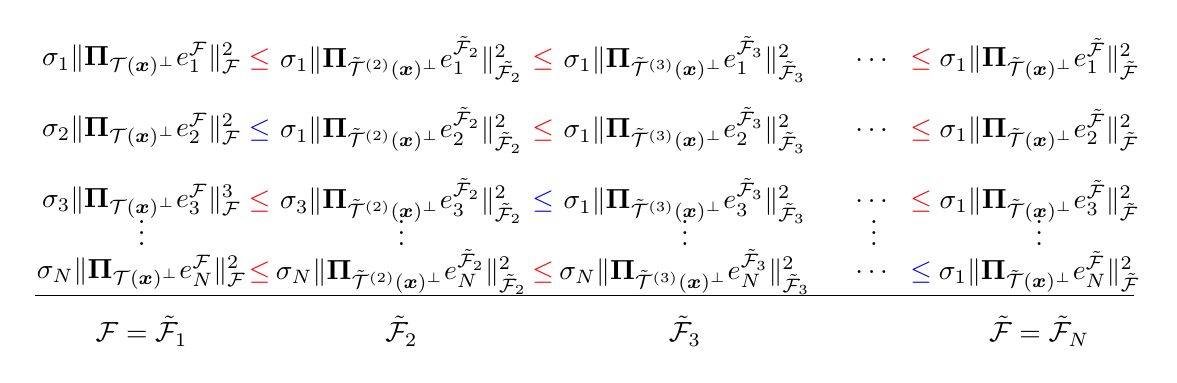
\begin{tikzpicture}[scale = 0.3]

  % draw line and angle
%  \draw 
%     pic [draw,angle radius=4mm,angle eccentricity=1.5, "$\theta$" font=\scriptsize] {angle=v2--v1--v3};

 

%\draw [fill=blue, opacity=0.5] (-15,3.75) -- (-11,3.75) -- (-11,5.5) -- (-15,5.5) -- (-15,3.75);
%\draw [fill=blue, opacity=0.5] (-15,3.5) -- (-11,3.5) -- (-11,3.75) -- (-15,3.75) -- (-15,3.5);
%\draw [fill=blue, opacity=0.5] (-15,3.25) -- (-11,3.25) -- (-11,3.5) -- (-15,3.5) -- (-15,3.25);
%\draw [fill=blue, opacity=0.5] (-15,4) -- (-11,4) -- (-11,3.25) -- (-15,3.25) -- (-15,4);
%\draw [fill=blue, opacity=0.5] (-15,2.75) -- (-11,2.75) -- (-11,4) -- (-15,4) -- (-15,2.75); 
%\draw [fill=blue, opacity=0.5] (-15,2.5) -- (-11,2.5) -- (-11,2.75) -- (-15,2.75) -- (-15,2.5);
%\draw [fill=blue, opacity=0.5] (-15,2.25) -- (-11,2.25) -- (-11,2.5) -- (-15,2.5) -- (-15,2.25);
%\draw [fill=blue, opacity=0.5] (-15,2) -- (-11,2) -- (-11,2.25) -- (-15,2.25) -- (-15,2);
%\draw [fill=blue, opacity=0.5] (-15,1.75) -- (-11,1.75) -- (-11,2) -- (-15,2) -- (-15,1.75);



%\draw [fill=blue, opacity=1] (-2,3.75) -- (2,3.75) -- (2,5.5) -- (-2,5.5) -- (-2,3.75);
%\draw [fill=blue, opacity=1] (-2,3.5) -- (2,3.5) -- (2,3.75) -- (-2,3.75) -- (-2,3.5);
%\draw [fill=blue, opacity=0.5] (-2,3.25) -- (2,3.25) -- (2,3.5) -- (-2,3.5) -- (-2,3.25);
%\draw [fill=blue, opacity=0.5] (-2,4) -- (2,4) -- (2,3.25) -- (-2,3.25) -- (-2,4);
%\draw [fill=blue, opacity=1] (-2,2.75) -- (2,2.75) -- (2,4) -- (-2,4) -- (-2,2.75); 
%\draw [fill=blue, opacity=0.5] (-2,2.5) -- (2,2.5) -- (2,2.75) -- (-2,2.75) -- (-2,2.5);
%\draw [fill=blue, opacity=0.5] (-2,2.25) -- (2,2.25) -- (2,2.5) -- (-2,2.5) -- (-2,2.25);
%\draw [fill=blue, opacity=1] (-2,2) -- (2,2) -- (2,2.25) -- (-2,2.25) -- (-2,2);
%\draw [fill=blue, opacity=0.5] (-2,1.75) -- (2,1.75) -- (2,2) -- (-2,2) -- (-2,1.75);





%\draw [fill=blue, opacity=1] (13,2.75) -- (17,2.75) -- (17,4) -- (13,4) -- (13,2.75);
%\draw [fill=blue, opacity=1] (13,2.5) -- (17,2.5) -- (17,2.75) -- (13,2.75) -- (13,2.5);
%\draw [fill=blue, opacity=1] (13,2.25) -- (17,2.25) -- (17,2.5) -- (13,2.5) -- (13,2.25);
%\draw [fill=blue, opacity=1] (13,2) -- (17,2) -- (17,2.25) -- (13,2.25) -- (13,2);


%\draw [fill=orange, opacity=1] (13.25,2) -- (13.25,2) -- (13.5,2) -- (13.5,4) -- (13.25,4);
%\draw [fill=orange, opacity=1] (14.25,2) -- (14.25,2) -- (14.5,2) -- (14.5,4) -- (14.25,4);
%\draw [fill=orange, opacity=1] (14.75,2) -- (14.75,2) -- (15,2) -- (15,4) -- (14.75,4);
%\draw [fill=orange, opacity=1] (15.75,2) -- (15.75,2) -- (16,2) -- (16,4) -- (15.75,4);



%\draw [->] (-7.5,2) --  (-6.5,2)  node [above] {\tiny $\Prb(T) \propto \prod_{i \in T} \sigma_{i}^{2}$} --  (-5.5,2);

%\draw [->] (6.5,2) --  (7.5,2)  node [above] {\tiny $\Prb(S|T) = \Det (\bm{V}_{S,T})^{2}$} --  (11.5,2);

%\draw  (-17,2.25)  node [above] {$\bm{V}^{\Tran}=$} ;

\draw  (-43,7)  node  {$\sigma_{1}\|\bm{\Pi}_{\mathcal{T}(\bm{x})^{\perp}}e_{1}^{\mathcal{F}}\|^{2}_{\mathcal{F}}$} ;
\draw  (-38,7)  node  {$\color{red} \leq$} ;
\draw  (-32,7)  node  {$\sigma_{1}\|\bm{\Pi}_{\tilde{\mathcal{T}}^{(2)}(\bm{x})^{\perp}}e_{1}^{\tilde{\mathcal{F}}_{2}}\|^{2}_{\tilde{\mathcal{F}_{2}}}$} ;
\draw  (-26,7)  node  {$\color{red} \leq$} ;
\draw  (-20,7)  node  {$\sigma_{1}\|\bm{\Pi}_{\tilde{\mathcal{T}}^{(3)}(\bm{x})^{\perp}}e_{1}^{\tilde{\mathcal{F}}_{3}}\|^{2}_{\tilde{\mathcal{F}}_{3}}$} ;
%\draw  (-20,7)  node  {$\leq$} ;
\draw  (-12,7)  node  {$\dots$} ;

\draw  (-10,7)  node  {$\color{red} \leq$} ;
\draw  (-5,7)  node  {$\sigma_{1}\|\bm{\Pi}_{\tilde{\mathcal{T}}(\bm{x})^{\perp}}e_{1}^{\tilde{\mathcal{F}}}\|^{2}_{\tilde{\mathcal{F}}}$} ;




\draw  (-43,4)  node  {$\sigma_{2}\|\bm{\Pi}_{\mathcal{T}(\bm{x})^{\perp}}e_{2}^{\mathcal{F}}\|^{2}_{\mathcal{F}}$} ;
\draw  (-38,4)  node  {$\color{blue} \leq$} ;
\draw  (-32,4)  node  {$\sigma_{1}\|\bm{\Pi}_{\tilde{\mathcal{T}}^{(2)}(\bm{x})^{\perp}}e_{2}^{\tilde{\mathcal{F}}_{2}}\|^{2}_{\tilde{\mathcal{F}}_{2}}$} ;
\draw  (-26,4)  node  {$\color{red} \leq$} ;
\draw  (-20,4)  node  {$\sigma_{1}\|\bm{\Pi}_{\tilde{\mathcal{T}}^{(3)}(\bm{x})^{\perp}}e_{2}^{\tilde{\mathcal{F}}_{3}}\|^{2}_{\tilde{\mathcal{F}}_{3}}$} ;
%\draw  (-20,7)  node  {$\leq$} ;
\draw  (-12,4)  node  {$\dots$} ;

\draw  (-10,4)  node  {$\color{red} \leq$} ;
\draw  (-5,4)  node  {$\sigma_{1}\|\bm{\Pi}_{\tilde{\mathcal{T}}(\bm{x})^{\perp}}e_{2}^{\tilde{\mathcal{F}}}\|^{2}_{\tilde{\mathcal{F}}}$} ;


\draw  (-43,1)  node  {$\sigma_{3}\|\bm{\Pi}_{\mathcal{T}(\bm{x})^{\perp}}e_{3}^{\mathcal{F}}\|^{3}_{\mathcal{F}}$} ;
\draw  (-38,1)  node  {$\color{red} \leq$} ;
\draw  (-32,1)  node  {$\sigma_{3}\|\bm{\Pi}_{\tilde{\mathcal{T}}^{(2)}(\bm{x})^{\perp}}e_{3}^{\tilde{\mathcal{F}}_{2}}\|^{2}_{\tilde{\mathcal{F}}_{2}}$} ;
\draw  (-26,1)  node  {$\color{blue} \leq$} ;
\draw  (-20,1)  node  {$\sigma_{1}\|\bm{\Pi}_{\tilde{\mathcal{T}}^{(3)}(\bm{x})^{\perp}}e_{3}^{\tilde{\mathcal{F}}_{3}}\|^{2}_{\tilde{\mathcal{F}}_{3}}$} ;
%\draw  (-20,7)  node  {$\leq$} ;
\draw  (-12,1)  node  {$\dots$} ;

\draw  (-10,1)  node  {$\color{red} \leq$} ;
\draw  (-5,1)  node  {$\sigma_{1}\|\bm{\Pi}_{\tilde{\mathcal{T}}(\bm{x})^{\perp}}e_{3}^{\tilde{\mathcal{F}}}\|^{2}_{\tilde{\mathcal{F}}}$} ;


\draw  (-43,0)  node  {$\vdots$} ;
%\draw  (-36,0)  node  {$\leq$} ;
\draw  (-32,0)  node  {$\vdots$} ;
%\draw  (-28,0)  node  {$\leq$} ;
\draw  (-20,0)  node  {$\vdots$} ;
%\draw  (-20,7)  node  {$\leq$} ;
\draw  (-12,0)  node  {$\vdots$} ;

%\draw  (-12,0)  node  {$\leq$} ;
\draw  (-5,0)  node  {$\vdots$} ;



\draw  (-43,-2)  node  {$\sigma_{N}\|\bm{\Pi}_{\mathcal{T}(\bm{x})^{\perp}}e_{N}^{\mathcal{F}}\|^{2}_{\mathcal{F}}$} ;
\draw  (-38,-2)  node  {$\color{red} \leq$} ;
\draw  (-32,-2)  node  {$\sigma_{N}\|\bm{\Pi}_{\tilde{\mathcal{T}}^{(2)}(\bm{x})^{\perp}}e_{N}^{\tilde{\mathcal{F}}_{2}}\|^{2}_{\tilde{\mathcal{F}}_{2}}$} ;
\draw  (-26,-2)  node  {$\color{red} \leq$} ;
\draw  (-20,-2)  node  {$\sigma_{N}\|\bm{\Pi}_{\tilde{\mathcal{T}}^{(3)}(\bm{x})^{\perp}}e_{N}^{\tilde{\mathcal{F}}_{3}}\|^{2}_{\tilde{\mathcal{F}}_{3}}$} ;
%\draw  (-20,7)  node  {$\leq$} ;
\draw  (-12,-2)  node  {$\dots$} ;

\draw  (-10,-2)  node  {$\color{blue} \leq$} ;
\draw  (-5,-2)  node  {$\sigma_{1}\|\bm{\Pi}_{\tilde{\mathcal{T}}(\bm{x})^{\perp}}e_{N}^{\tilde{\mathcal{F}}}\|^{2}_{\tilde{\mathcal{F}}}$} ;

\draw[line width=0.15 mm] (-47.5,-3) -- (-1,-3);

\draw  (-43,-4.5)  node  {$\mathcal{F}=\tilde{\mathcal{F}}_{1}$} ;
\draw  (-38,-4.5)  node  {} ;
\draw  (-32,-4.5)  node  {$\tilde{\mathcal{F}}_{2}$} ;
\draw  (-26,-4.5)  node  {} ;
\draw  (-20,-4.5)  node  {$\tilde{\mathcal{F}}_{3}$} ;
%\draw  (-20,7)  node  {$\leq$} ;
\draw  (-12,-4.5)  node  {} ;

\draw  (-10,-4.5)  node  {} ;
\draw  (-5,-4.5)  node  {$\tilde{\mathcal{F}} = \tilde{\mathcal{F}}_{N}$} ;
\end{tikzpicture}

% \pc{Peut-être introduire $\Delta_n^{\cal F}(\bm{x}) = e_{n}^{\mathcal{F}}(\bm{x})^{\Tran}\bm{K}(\bm{x})^{-1}e_{n}^{\mathcal{F}}(\bm{x})$ et  $\Delta_n^{\tilde{\cal F}_\ell}(\bm{x}) = e_{n}^{\tilde{\mathcal{F}}_{\ell}}(\bm{x})^{\Tran}\tilde{\bm{K}}^{(\ell)}(\bm{x})^{-1}e_{n}^{\tilde{\mathcal{F}}_{\ell}}(\bm{x})$ pour alléger l'écriture avec $\l...\l$ partout ?}
% %\subfloat[]{\includegraphics{img/BernoulliKernels/Bernoulli_kernels_same_node_s_1_5_zoom.pdf}} \\
% \caption{The illustration of the inequalities in Proposition~\ref{prop:graded_RKHS}. The inequality \eqref{eq:graded_RKHS_inequality_1} is in blue and the inequality \eqref{eq:graded_RKHS_inequality_2} is in red. \label{fig:graded_RKHS}}
% \end{figure}



%%%%%%%% Proposition 3 : a) Proposition 2, b) Lemma 2, c) Lemma 4, d) Lemma 5

\subsection{Proof of Proposition~\ref{prop:expected_value_of_product_of_cos}}
\label{s:proofOfExpectedProduct}
% Remark
%\subsection{A bound for $\displaystyle \EX_{\DPP} \prod\limits_{\ell \in [N]} \frac{1}{\cos^{2} \theta_{\ell}\left(\mathcal{E}^{\mathcal{F}}_{N}, \mathcal{T}(x) \right)}$}
%\pc{Revoir titre : j'ai enlevé le titre "A bound for $\displaystyle \EX_{\DPP} \prod\limits_{\ell \in [N]} \frac{1}{\cos^{2} \theta_{\ell}\left(\mathcal{E}^{\mathcal{F}}_{N}, \mathcal{T}(x) \right)}$"}
%

In this section, $\bm{x}  = (x_{1}, \dots , x_{N}) \in \mathcal{X}^{N}$ is the realization of the DPP of Theorem~\ref{thm:main_theorem}. Let $\bm{E}^{\mathcal{F}}(\bm{x}) = (e_{i}^{\mathcal{F}}(x_{j}))_{1 \leq i,j \leq N}$ and $\bm{E}(\bm{x}) = (e_{i}(x_{j}))_{1 \leq i,j \leq N}$, and $\bm{K}(\bm{x})= (k(x_{i},x_{j}))_{1 \leq i,j \leq N} $.
Moreover, let $\mathcal{E}^{\mathcal{F}}_{N} = \Span(e_{m}^{\mathcal{F}})_{m \in [N]}$ and $\mathcal{T}(\bm{x}) =  \Span \left( k(x_{i},.) \right)_{i \in [N]}$.

We first prove two lemmas that are necessary to prove Proposition~\ref{prop:expected_value_of_product_of_cos}.

%%%
\subsubsection{Two preliminary lemmas}

%%% Lemma 4
%%%%%%
\begin{lemma}\label{lemma:cos_ratio_det}
Let $\bm{x} =  (x_{1}, \dots , x_{N}) \in \mathcal{X}^{N} $ such that $\Det^{2} \bm{E}(\bm{x}) \neq 0$. Then,
\begin{equation}
\prod\limits_{\ell \in [N]} \frac{1}{\cos^{2} \theta_{\ell} \left(\mathcal{E}^{\mathcal{F}}_{N}, \mathcal{T}(\bm{x}) \right)} = \frac{\Det \bm{K}(\bm{x})}{\Det^{2} \bm{E}^{\mathcal{F}}(\bm{x})}.
\end{equation}
\end{lemma}

\begin{proof}
The condition $\Det^{2} \bm{E}(\bm{x}) \neq 0$ yields by Proposition~\ref{prop:K_N_non_singular} that $\bm{K}(\bm{x})$ is non singular. Thus $\dim \mathcal{T}(\bm{x}) = N$. Let $(t_{i})_{i \in [N]}$ an orthonormal basis of $\mathcal{T}(\bm{x})$ with respect to $\langle ., . \rangle_{\mathcal{F}}$.
%
Using Proposition~\ref{prop:cos_det_relationship}, and the fact that $(e_{n}^{\mathcal{F}})_{n \in [N]}$ is an orthonormal basis of $\mathcal{E}^{\mathcal{F}}_{N}$ according to $\langle ., . \rangle_{\mathcal{F}}$,
\begin{equation}\label{eq:prod_cos_det_E}
\prod\limits_{\ell \in [N]} \cos^{2} \theta_{\ell} \left(\mathcal{E}^{\mathcal{F}}_{N}, \mathcal{T}(\bm{x}) \right) = \Det^{2} (\langle e_{n}^{\mathcal{F}}, t_{i} \rangle_{\mathcal{F}})_{(n,i) \in [N]\times[N]}.
\end{equation}
Now, write for $i \in [N]$,
\begin{equation}\label{eq:t_as_function_of_kx}
t_{i} = \sum\limits_{j \in [N]} c_{i,j} k(x_{j},.).
\end{equation}
%
Thus
\begin{align}
\langle e_{n}^{\mathcal{F}}, t_{i} \rangle_{\mathcal{F}} = & \sum\limits_{j \in [N]} c_{i,j} \langle e_{n}^{\mathcal{F}}, k(x_{j},.) \rangle_{\mathcal{F}} \\
= &\sum\limits_{j \in [N]} c_{i,j}  e_{n}^{\mathcal{F}}(x_{j}).
\end{align}
%
Then
\begin{equation}
(\langle e_{n}^{\mathcal{F}}, t_{i} \rangle_{\mathcal{F}})_{(n,i) \in [N]\times[N]} = \bm{E}^{\mathcal{F}}(\bm{x}) \bm{C}(\bm{x})^{\Tran} ,
\end{equation}
where
\begin{equation}
\bm{C}(\bm{x}) = (c_{i,j})_{1 \leq i,j \leq N}.
\end{equation}
%
Thus
\begin{equation}\label{eq:AN_times_EN}
\Det^{2} (\langle e_{n}^{\mathcal{F}}, t_{i} \rangle_{\mathcal{F}})_{(n,i) \in [N]\times[N]} = \Det^{2} \bm{C}(\bm{x}) \Det^{2} \bm{E}^{\mathcal{F}}(\bm{x}).
\end{equation}
%%%%
Now, let $\bm{c}_{i}$ the columns of the matrix $\bm{C}(\bm{x})$. $(t_{i})_{i \in [N]}$ is an orthonormal basis of $\mathcal{T}(\bm{x})$ with respect to $\langle .,. \rangle_{\mathcal{F}}$, then by \eqref{eq:t_as_function_of_kx}
\begin{equation}
  \delta_{i,i'} = \langle t_{i}, t_{i'} \rangle_{\mathcal{F}} = \bm{c}_{i}^{\Tran} \bm{K}(\bm{x}) \bm{c}_{i'}  .
\end{equation}
Therefore
\begin{equation}
\bm{C}(\bm{x})^{\Tran} \bm{K}(\bm{x}) \bm{C}(\bm{x}) = \mathbb{I}_{N}.
\end{equation}
Thus
\begin{equation}\label{eq:det_AN_det_KN_relationship}
\Det^{2} \bm{C}(\bm{x}) = \frac{1}{\Det \bm{K}(\bm{x})}.
\end{equation}
Combining \eqref{eq:prod_cos_det_E}, \eqref{eq:AN_times_EN} and \eqref{eq:det_AN_det_KN_relationship} concludes the proof of Lemma~\ref{lemma:cos_ratio_det}:
\begin{equation}
\prod\limits_{\ell \in [N]} \frac{1}{\cos^{2} \theta_{\ell} \left(\mathcal{E}^{\mathcal{F}}_{N}, \mathcal{T}(\bm{x}) \right)} = \frac{\Det \bm{K}(\bm{x})}{\Det^{2} \bm{E}^{\mathcal{F}}(\bm{x})}.
\end{equation}
\end{proof}



%%%%%% Lemma 5
\begin{lemma}\label{lemma:truncated_Fredholm_formula}
\begin{equation}
  \frac{1}{N!} \int_{\mathcal{X}^{N}}\Det \bm{K}(x_{1}, \dots, x_{N}) \otimes_{j \in [N]} \mathrm{d}\omega(x_{j})  = \sum\limits_{\substack{T \subset \mathbb{N}^{*} \\ |T| = N}}  \prod\limits_{t \in T}\sigma_{t}.
\end{equation}
\end{lemma}
%% Proof
\begin{proof}
Let $\bm{x} = (x_{1}, \dots, x_{N}) \in \mathcal{X}^{N}$. From \eqref{eq:truncated_kernel_limit}
\begin{equation}
\Det \bm{K}(\bm{x}) = \lim\limits_{M \rightarrow \infty} \Det \bm{K}_{M}(\bm{x}).
\end{equation}
Moreover,
\begin{equation}
\Det \bm{K}_{M}(\bm{x})  = \sum\limits_{T \subset [M], |T| = N} \prod\limits_{i \in T} \sigma_{i} \Det^{2} (e_{i}(x_{j}))_{(i,j)\in T \times [N]}.
\end{equation}
Now, for $T \subset [M]$ such that $|T| = N$, $(e_{t})_{t \in T}$ is an orthonormal family of $\mathbb{L}_{2}(\mathrm{d}\omega)$, then by \cite{HoKrPeVi06} Lemma 21:
\begin{equation}
\int_{\mathcal{X}^{N}}\Det^{2} (e_{t}(x_{j})) \otimes_{j \in [N]} \mathrm{d}\omega(x_{j}) = N! .
\end{equation}

Thus
\begin{align}
\frac{1}{N!} \int_{\mathcal{X}^{N}}\Det \bm{K}_{M}(\bm{x}) \otimes_{j \in [N]} \mathrm{d}\omega(x_{j}) &=  \frac{1}{N!} \sum\limits_{T \subset [M], |T| = N} \prod\limits_{t \in T} \sigma_{t} \int_{\mathcal{X}^{N}}\Det^{2} (e_{t}(x_{j})) \otimes_{j \in [N]} \mathrm{d}\omega(x_{j}) \\
& = \sum\limits_{T \subset [M], |T| = N} \prod\limits_{t \in T} \sigma_{t} \nonumber.
\end{align}
Now, $\displaystyle \sum\limits_{n \in \mathbb{N}^{*}} \sigma_{n} < \infty$ implies that $\displaystyle \sum\limits_{T \subset \mathbb{N}^{*}, |T| = N} \prod\limits_{t \in T} \sigma_{t} < \infty$. In fact, for $\ell \in [N]$ let $p_{\ell}$ the $\ell$-th symmetric polynomial. By Maclaurin’s inequality \citep{Ste04}, and for any vector $\bm{\nu} \in \mathbb{R}_{+}^{M}$
\begin{equation}
\left( \frac{p_{\ell}(\bm{\nu})}{{M\choose \ell}} \right)^{\frac{1}{\ell}} \leq \frac{p_{1}(\bm{\nu})}{M}.
\end{equation}
Thus
\begin{align}\label{eq:Maclaurin_inequality}
p_{\ell}(\bm{\nu}) & \leq  \frac{{M\choose \ell}}{M^{\ell}}p_{1}(\bm{\nu})^{\ell} \\
& \leq \frac{M!}{\ell!(M-\ell)! M^{\ell}}p_{1}(\bm{\nu})^{\ell} \nonumber\\
& \leq \frac{M (M-1) \dots (M-\ell +1)}{\ell! M^{\ell}}p_{1}(\bm{\nu})^{\ell} \nonumber\\
& \leq \frac{1}{\ell !}p_{1}(\bm{\nu})^{\ell} \nonumber.
\end{align}
This inequality is independent of the dimension $M$ thus it can be extended for $\bm{\nu} \in \mathbb{R}_{+}^{\mathbb{N}^{*}}$ with $\displaystyle \sum\limits_{n \in \mathbb{N}^{*}} \nu_{n} < \infty$. Therefore
\begin{equation}
\sum\limits_{T \subset \mathbb{N}^{*}, |T| = N} \prod\limits_{t \in T} \sigma_{t}  \leq \frac{1}{N!} (\sum\limits_{n \in \mathbb{N}^{*}} \sigma_{n})^{N} < \infty .
\end{equation}

Furthermore,
\begin{equation}
\forall M \in \mathbb{N}^{*}, \: \forall \bm{x} \in \mathcal{X}^{N}, \: 0 \leq \Det \bm{K}_{M}(\bm{x}) \leq \Det \bm{K}_{M+1,N}(\bm{x}).
\end{equation}
Then by monotone convergence theorem, $\displaystyle \bm{x} \mapsto \frac{1}{N!}\Det \bm{K}(\bm{x})$ is mesurable and
\begin{align}
\int_{\mathcal{X}^{N}} \frac{1}{N!}\Det \bm{K}(\bm{x}) \otimes_{j \in [N]} \mathrm{d}\omega(x_j) & = \lim\limits_{M \rightarrow \infty} \int_{\mathcal{X}^{N}}\frac{1}{N!} \Det \bm{K}_{M}(\bm{x})\otimes_{j \in [N]} \mathrm{d}\omega(x_j)\\
& = \lim\limits_{M \rightarrow \infty} \sum\limits_{T \subset [M], |T| = N} \prod\limits_{t \in T} \sigma_{t} \nonumber\\
& = \sum\limits_{T \subset \mathbb{N}^{*}, |T| = N} \prod\limits_{t \in T} \sigma_{t} \nonumber.
\end{align}
% thanks to the convergence of $\displaystyle \sum\limits_{n \in \mathbb{N}} \sigma_{n} < \infty$.
\end{proof}

%%%%%%%%%%%%%%%% Proposition 3
\subsubsection{End of the proof of Proposition~\ref{prop:expected_value_of_product_of_cos}}
%Now we can prove Proposition~\ref{prop:expected_value_of_product_of_cos} thanks to Lemmas~\ref{lemma:cos_ratio_det} \& \ref{lemma:truncated_Fredholm_formula} above.
\begin{proof}
Remember that
\begin{equation}
\Prb \left( \Det \bm{E}(\bm{x})  \neq 0 \right) = 1.
\end{equation}
Then by Lemma~\ref{lemma:cos_ratio_det} and the fact that $\Det^{2} \bm{E}^{\mathcal{F}}(\bm{x}) = \prod\limits_{n \in [N]} \sigma_{n} \Det^{2} \bm{E}(\bm{x})$
\begin{equation}
\prod\limits_{\ell \in [N]} \frac{1}{\cos^{2} \theta_{\ell} \left(\mathcal{E}^{\mathcal{F}}_{N}, \mathcal{T}(\bm{x}) \right)} = \frac{\Det \bm{K}(\bm{x})}{\Det^{2} \bm{E}^{\mathcal{F}}(\bm{x})} = \frac{1}{\prod\limits_{n \in [N]} \sigma_{n}}\frac{\Det \bm{K}(\bm{x})}{\Det^{2} \bm{E}(\bm{x})}.
\end{equation}
Then, taking the expectation with respect to $\bm{x}$ resulting from a DPP of kernel $\KDPP(x,y)$,
\begin{align}
\EX_{\DPP} \prod\limits_{\ell \in [N]} \frac{1}{\cos^{2} \theta_{\ell}\left(\mathcal{E}^{\mathcal{F}}_{N}, \mathcal{T}(\bm{x}) \right)} = & \frac{1}{N!} \int_{\mathcal{X}^{N}} \Det^{2} \bm{E}(\bm{x}) \prod\limits_{\ell \in [N]} \frac{1}{\cos^{2} \theta_{\ell} \left(\mathcal{E}^{\mathcal{F}}_{N}, \mathcal{T}(\bm{x}) \right)} \otimes_{i =1}^{N} \mathrm{d}\omega(x_{i}) \\
 = & \frac{1}{N!} \int_{\mathcal{X}^{N}} \Det^{2} \bm{E}(\bm{x}) \frac{1}{\prod\limits_{n \in [N]} \sigma_{n}}\frac{\Det \bm{K}(\bm{x})}{\Det^{2} \bm{E}(\bm{x})} \otimes_{i =1}^{N} \mathrm{d}\omega(x_{i}) \nonumber\\
 = & \frac{1}{\prod\limits_{n \in [N]} \sigma_{n}} \frac{1}{N!} \int_{\mathcal{X}^{N}}\Det \bm{K}(\bm{x}) \otimes_{i =1}^{N} \mathrm{d}\omega(x_{i}) \nonumber.
\end{align}
Now, by Lemma~\ref{lemma:truncated_Fredholm_formula}
\begin{equation}
\frac{1}{N!} \int_{\mathcal{X}^{N}}\Det \bm{K}(\bm{x}) \otimes_{i =1}^{N} \mathrm{d}\omega(x_{i})  = \sum\limits_{\substack{T \subset \mathbb{N}^{*} \\ |T| = N}}  \prod\limits_{t \in T}\sigma_{t}.
\end{equation}
Therefore,
\begin{equation}
\EX_{\DPP} \prod\limits_{\ell \in [N]} \frac{1}{\cos^{2} \theta_{\ell}\left(\mathcal{E}^{\mathcal{F}}_{N}, \mathcal{T}(\bm{x}) \right)}  =  \sum\limits_{\substack{T \subset \mathbb{N}^{*} \\ |T| = N}} \frac{ \prod\limits_{t \in T}\sigma_{t}}{\prod\limits_{n \in [N]} \sigma_{n}}.
\end{equation}

\end{proof}


%%%%%%%% Theorem 1
%%%%%%%%%%%%%%%%%% Main Theorem
\subsection{Proof of Theorem~\ref{thm:main_theorem}}
\label{s:finalBound}
\begin{proof}
Thanks to Proposition~\ref{prop:kernel_perturbation_inequality} and Lemma~\ref{lemma:max_error_cos} (for $\tilde{\cal F}$ and $\tilde{k}$)
\begin{align}\label{eq:prooftheorem1_first}
  \max_{ n \in [N]}\sigma_n \|\bm{\Pi}_{\mathcal{T}(\bm{x})^{\perp}} e_{n}^{\mathcal{F}}\|_{\mathcal{F}}^{2}
  & \leq
  \sigma_1 \cdot \max_{ n \in [N]} \|\bm{\Pi}_{\tilde{\cal{T}}(\bm{x})^{\perp}} e_{n}^{\tilde{\mathcal{F}}}\|_{\tilde{\mathcal{F}}}^{2}\\
  & \leq
  \sigma_1 \cdot \left( \prod\limits_{n \in [N]}\frac{1}{\cos^{2} \theta_{n}(\tilde{\cal{T}}(\bm{x}),\mathcal{E}^{\tilde{\mathcal{F}}}_{N})} - 1\right).
\end{align}
%
%\begin{equation}
% \EX_{\DPP} \prod\limits_{\ell \in [N]} \frac{1}{\cos^{2} \theta_{\ell}\left(\mathcal{E}^{\tilde{\mathcal{F}}}_{N}, \tilde{\mathcal{T}}_{N}(\bm{x}) \right)}  \leq \EX_{\DPP} \prod\limits_{\ell \in [N]} \frac{1}{\cos^{2} \theta_{\ell}\left(\mathcal{E}^{\tilde{\mathcal{F}}}_{N}, \tilde{\mathcal{T}}_{N}(\bm{x}) \right)}
%\end{equation}
%
Then Proposition~\ref{prop:expected_value_of_product_of_cos} applied to $\tilde{\cal F}$ with kernel $\tilde{k}$ yields
\begin{equation}
  \EX_{\DPP} \prod\limits_{n \in [N]} \frac{1}{\cos^{2} \theta_{n}\left(\mathcal{E}^{\tilde{\mathcal{F}}}_{N}, \tilde{\mathcal{T}}_{N}(\bm{x}) \right)}   =
  \sum\limits_{\substack{T \subset \mathbb{N}^{*} \\ |T| = N}} \frac{ \prod\limits_{t \in T}\tilde{\sigma}_{t}}{\prod\limits_{n \in [N]} \tilde{\sigma}_{n}}.
\end{equation}
%
Every subset $T \subset \mathbb{N}^{*}$ such that $|T| = N$ can be written as $T = V \cup W$ with $V \subset [N]$ and $W \subset \mathbb{N}^{*} \smallsetminus [N]$, and this decomposition is unique. Then
\begin{equation}
\frac{ \prod\limits_{t \in T}\tilde{\sigma}_{t}}{\prod\limits_{n \in [N]} \tilde{\sigma}_{n}} = \frac{\prod\limits_{v \in V}\tilde{\sigma}_{v} \prod\limits_{w \in W}\tilde{\sigma}_{w}}{\prod\limits_{n \in [N]} \tilde{\sigma}_{n}} = \frac{\prod\limits_{w \in W}\tilde{\sigma}_{w}}{\prod\limits_{n \in [N]\smallsetminus V} \tilde{\sigma}_{n}}.
\end{equation}
Therefore
\begin{align}
  \sum\limits_{\substack{T \subset \mathbb{N}^{*} \\ |T| = N}} \frac{ \prod\limits_{t \in T}\tilde{\sigma}_{t}}{\prod\limits_{n \in [N]} \tilde{\sigma}_{n}} & = \sum\limits_{\substack{T \subset \mathbb{N}^{*} \\ |T| = N\\ T = V \cup W}} \frac{\prod\limits_{w \in W}\tilde{\sigma}_{w}}{\prod\limits_{n \in [N]\smallsetminus V} \tilde{\sigma}_{n}} \\
  & = \sum\limits_{V \subset [N]}\sum\limits_{\substack{W \subset \mathbb{N}^{*}\smallsetminus [N]\\ |W| = N-|V|}} \frac{\prod\limits_{w \in W}\tilde{\sigma}_{w}}{\prod\limits_{n \in [N]\smallsetminus V} \tilde{\sigma}_{n}} \nonumber\\
  & = \sum\limits_{0 \leq \ell \leq N} \bigg[ \sum\limits_{\substack{V \subset [N]\\ |V| = \ell}}\prod\limits_{n \in [N]\smallsetminus V} \frac{1}{\tilde{\sigma}_{n}}\bigg]\bigg[\sum\limits_{\substack{W \subset \mathbb{N}^{*}\smallsetminus [N]\\ |W| = N-\ell}} \prod\limits_{w \in W}\tilde{\sigma}_{w}\bigg] \nonumber\\
  & = \sum\limits_{0 \leq \ell \leq N} \bigg[\sum\limits_{\substack{V \subset [N]\\ |V| = N-\ell}}\prod\limits_{n \in V} \frac{1}{\tilde{\sigma}_{n}}\bigg] \bigg[\sum\limits_{\substack{W \subset \mathbb{N}^{*}\smallsetminus [N]\\ |W| = N-\ell}} \prod\limits_{w \in W}\tilde{\sigma}_{w}\bigg] \nonumber\\
  & = \sum\limits_{0 \leq \ell \leq N} p_{N-\ell}\left(\left(\frac{1}{\tilde{\sigma}_{m}}\right)_{m \in [N]}\right)p_{N-\ell}\left((\tilde{\sigma}_{m})_{m \geq N+1}\right) \nonumber\\
  & = \sum\limits_{0 \leq \ell \leq N} p_{\ell}\left(\left(\frac{1}{\tilde{\sigma}_{m}}\right)_{m \in [N]}\right)p_{\ell}\left((\tilde{\sigma}_{m})_{m \geq N+1}\right) \nonumber,
\end{align}
where for $\ell \in [N]$, $p_{\ell}$ is the $\ell$-th symmetric polynomial with the convention that $p_{0} = 1$.

%
Finally, thanks to \eqref{eq:Maclaurin_inequality} above
\begin{align}
  \sum\limits_{\substack{T \subset \mathbb{N}^{*} \\ |T| = N}} \frac{ \prod\limits_{t \in T}\tilde{\sigma}_{t}}{\prod\limits_{n \in [N]} \tilde{\sigma}_{n}}
  & \leq  1 + \sum\limits_{\ell \in [N]} \frac{1}{\ell!^{2}} \left(\sum\limits_{m \in [N]}\frac{1}{\tilde{\sigma}_{m}} \sum\limits_{m \geq N+1} \tilde{\sigma}_{m}\right)^{\ell} \\
  & \leq 1+ \sum\limits_{\ell \in [N]} \frac{1}{\ell!^{2}} \left(\frac{N}{\sigma_1} \sum\limits_{m \geq N+1} \sigma_{m}\right)^{\ell} \nonumber.
\end{align}
%
As a consequence, by writing $r_{N} = \sum\limits_{m \geq N+1} \sigma_{m}$,
\begin{equation}
  \EX_{\DPP} \left[ \max_{ n \in [N]}\sigma_n \|\bm{\Pi}_{\mathcal{T}(\bm{x})^{\perp}} e_{n}^{\mathcal{F}}\|_{\mathcal{F}}^{2} \right]
  \leq
  \sigma_1 \cdot \sum_{\ell=1}^{N} \frac{1}{\ell!^{2}} \left(\frac{N  r_{N} }{\sigma_1}\right)^{\ell}
% \sigma_1 \cdot \sum_{\ell=1}^{N} \frac{1}{\ell!^{2}} \left(\frac{N}{\sigma_1} \sum\limits_{m \geq N+1} \sigma_{m}\right)^{\ell}
\end{equation}
which can be plugged in Lemma~\ref{lemma:approximation_error_spectral_bound} to conclude the proof.
\end{proof}


\subsection{The proofs of the strong version}
Our objective in this section is to give a tractable expression of 
\begin{equation}
\EX_{\DPP} \sum\limits_{\ell \in [N]} \frac{1}{\cos^{2} \theta_{\ell} \bigg(\mathcal{E}^{\mathcal{F}}_{N}, \mathcal{T}(\bm{x}) \bigg)}.
\end{equation}
We start by proving the following result.
%%%%%%
\begin{lemma}\label{lemma:sum_inverse_cos}
Let $\bm{x} =  (x_{1}, \dots , x_{N}) \in \mathcal{X}^{N} $ such that $\Det^{2} \bm{E}(\bm{x}) \neq 0$. Then,
\begin{equation}
\sum\limits_{\ell \in [N]} \frac{1}{\cos^{2} \theta_{\ell} \bigg(\mathcal{E}^{\mathcal{F}}_{N}, \mathcal{T}(\bm{x}) \bigg)} = \Tr \bigg(\bm{E}^{\mathcal{F}}(\bm{x})^{\Tran^{-1}}  \bm{K}(\bm{x}) \bm{E}^{\mathcal{F}}(\bm{x})^{-1} \bigg).
\end{equation}
\end{lemma}

\begin{proof}
We proceed as in the proof of Lemma~\ref{lemma:cos_ratio_det}. 
The condition $\Det^{2} \bm{E}(\bm{x}) \neq 0$ yields by Proposition~\ref{prop:K_N_non_singular} that $\bm{K}(\bm{x})$ is non singular. Thus $\dim \mathcal{T}(\bm{x}) = N$. Let $(t_{i})_{i \in [N]}$ be an orthonormal basis of $\mathcal{T}(\bm{x})$ with respect to $\langle ., . \rangle_{\mathcal{F}}$ and let $\bm{W}(\bm{x}) = \langle e_{n}^{\mathcal{F}}, t_{i} \rangle_{\mathcal{F}}$.
%
Using Proposition~\ref{prop:cos_det_relationship}, and the fact that $(e_{n}^{\mathcal{F}})_{n \in [N]}$ is an orthonormal basis of $\mathcal{E}^{\mathcal{F}}_{N}$ with respect to $\langle ., . \rangle_{\mathcal{F}}$, the $\cos^{2} \theta_{\ell} \bigg(\mathcal{E}^{\mathcal{F}}_{N}, \mathcal{T}(\bm{x}) \bigg)$ are the eigenvalues of the matrix $\bm{W}(\bm{x})\bm{W}(\bm{x})^{\Tran}$. Thus
\begin{equation}\label{eq:sum_cos_tr_E}
\sum\limits_{\ell \in [N]} \frac{1}{\cos^{2} \theta_{\ell} \bigg(\mathcal{E}^{\mathcal{F}}_{N}, \mathcal{T}(\bm{x}) \bigg)} = \Tr \bigg( \bm{W}(\bm{x})\bm{W}(\bm{x})^{\Tran} \bigg)^{-1}.
\end{equation}
Now, using the same analysis as in the proof of Lemma~\ref{lemma:cos_ratio_det}, we get 


% Now, write for $i \in [N]$,
% \begin{equation}\label{eq:t_as_function_of_kx}
% t_{i} = \sum\limits_{j \in [N]} c_{j,i} k(x_{j},.).
% \end{equation}
% %
% Thus
% \begin{align}
% \langle e_{n}^{\mathcal{F}}, t_{i} \rangle_{\mathcal{F}} = & \sum\limits_{j \in [N]} c_{j,i} \langle e_{n}^{\mathcal{F}}, k(x_{j},.) \rangle_{\mathcal{F}} \\
% = &\sum\limits_{j \in [N]}e_{n}^{\mathcal{F}}(x_{j}) c_{j,i}.
% \end{align}
% %
% Then
\begin{equation}
\bm{W}(\bm{x}) = \bm{E}^{\mathcal{F}}(\bm{x})\bm{C}(\bm{x}) ,
\end{equation}
where
\begin{equation}
\bm{C}(\bm{x})^{\Tran} \bm{K}(\bm{x}) \bm{C}(\bm{x}) = \mathbb{I}_{N}.
\end{equation}

%
Thus
\begin{align}\label{eq:AN_times_EN}
\bigg( \bm{W}(\bm{x})\bm{W}(\bm{x})^{\Tran} \bigg)^{-1} & = \bm{E}^{\mathcal{F}}(\bm{x})^{\Tran^{-1}} \bigg( \bm{C}(\bm{x})\bm{C}(\bm{x})^{\Tran} \bigg)^{-1}  \bm{E}^{\mathcal{F}}(\bm{x})^{-1} \nonumber \\
& = \bm{E}^{\mathcal{F}}(\bm{x})^{\Tran^{-1}} \bm{K}(\bm{x}) \bm{E}^{\mathcal{F}}(\bm{x})^{-1}
\end{align}
Combining \eqref{eq:sum_cos_tr_E} and \eqref{eq:AN_times_EN} concludes the proof of Lemma~\ref{lemma:sum_inverse_cos}:
\begin{equation}
\sum\limits_{\ell \in [N]} \frac{1}{\cos^{2} \theta_{\ell} \bigg(\mathcal{E}^{\mathcal{F}}_{N}, \mathcal{T}(\bm{x}) \bigg)} = \Tr \bigg(\bm{E}^{\mathcal{F}}(\bm{x})^{\Tran^{-1}} \bm{K}(\bm{x})  \bm{E}^{\mathcal{F}}(\bm{x})^{-1} \bigg).
\end{equation}
\end{proof}
Now, we are ready to prove Theorem~\ref{thm:ex_dpp_sum_inv_cos}
\paragraph{Proof of Theorem ~\ref{thm:ex_dpp_sum_inv_cos}}

% We use the following result proved in []
% \begin{lemma} \label{lemma:det_tr_delta_0}
% Let $\bm{A}, \bm{B} \in \mathbb{R}^{N \times N}$ two matrices with the same dimension. Assume that $\Det~\bm{A}~\neq~0$, then
% \begin{equation}
% \partial_{t} \Det (\bm{A}+t\bm{B})_{|t = 0} = \Det(\bm{A}) \Tr(\bm{A}^{-1}\bm{B}).  
% \end{equation} 
% \end{lemma}

% \Tr \bigg(  \bm{E}^{\mathcal{F}}(\bm{x})^{\Tran^{-1}}\bm{K}(\bm{x})\bm{E}^{\mathcal{F}}(\bm{x})^{-1} \bigg)
Define $I_{k,N}$ by
\begin{equation}
I_{k,N} = \EX_{\DPP} \sum\limits_{\ell \in [N]} \frac{1}{\cos^{2} \theta_{\ell} \bigg(\mathcal{E}^{\mathcal{F}}_{N}, \mathcal{T}(\bm{x}) \bigg)}.
\end{equation}
By Lemma~\ref{lemma:sum_inverse_cos}, we have
\begin{equation}
\sum\limits_{\ell \in [N]} \frac{1}{\cos^{2} \theta_{\ell} \bigg(\mathcal{E}^{\mathcal{F}}_{N}, \mathcal{T}(\bm{x}) \bigg)} = \Tr \bigg(  \bm{E}^{\mathcal{F}}(\bm{x})^{\Tran^{-1}}\bm{K}(\bm{x})\bm{E}^{\mathcal{F}}(\bm{x})^{-1} \bigg).
\end{equation}
Therefore,
\begin{align}\label{eq:I_k_N}
 I_{k,N} & = \frac{1}{N!} \int_{\mathcal{X}^{N}} \Det^{2}\bm{E}(\bm{x}) \Tr \bigg( \bm{E}^{\mathcal{F}}(\bm{x})^{\Tran^{-1}} \bm{K}(\bm{x}) \bm{E}^{\mathcal{F}}(\bm{x})^{-1}\bigg) \otimes_{j \in [N]} \mathrm{d}\omega(x_{j}) \nonumber\\
& = \frac{1}{N!} \int_{\mathcal{X}^{N}} \Det^{2}\bm{E}(\bm{x}) \Tr \bigg(\bm{E}^{\mathcal{F}}(\bm{x})^{-1} \bm{E}^{\mathcal{F}}(\bm{x})^{\Tran^{-1}} \bm{K}(\bm{x}) \bigg) \otimes_{j \in [N]} \mathrm{d}\omega(x_{j}) \nonumber\\
& = \frac{1}{N!} \int_{\mathcal{X}^{N}} \Det^{2}\bm{E}(\bm{x}) \Tr \bigg(\big(\bm{E}^{\mathcal{F}}(\bm{x})^{\Tran}\bm{E}^{\mathcal{F}}(\bm{x})\big)^{-1}  \bm{K}(\bm{x}) \bigg) \otimes_{j \in [N]} \mathrm{d}\omega(x_{j}) \nonumber\\
& = \frac{1}{N!\prod\limits_{n \in [N]}\sigma_{n}} \int_{\mathcal{X}^{N}} \Det^{2}\bm{E}^{\mathcal{F}}(\bm{x}) \Tr \bigg(\big(\bm{E}^{\mathcal{F}}(\bm{x})^{\Tran}\bm{E}^{\mathcal{F}}(\bm{x})\big)^{-1}  \bm{K}(\bm{x}) \bigg) \otimes_{j \in [N]} \mathrm{d}\omega(x_{j}).
\end{align}
Now, let $\bm{x} \in \mathcal{X}^{N}$ such that $\Det \bm{E}(\bm{x}) \neq 0$. Then, by Lemma~\ref{lemma:det_tr_delta_0}
\begin{equation}
 \Det^{2} \bm{E}^{\mathcal{F}}(\bm{x}) \Tr \bigg(\Big(\bm{E}^{\mathcal{F}}(\bm{x})^{\Tran}\bm{E}^{\mathcal{F}}(\bm{x})\Big)^{-1}\bm{K}(x)\bigg) = \partial_{t} \Det \bigg(\bm{E}^{\mathcal{F}}(\bm{x})^{\Tran}\bm{E}^{\mathcal{F}}(\bm{x})+t\bm{K}(x)\bigg)_{|t = 0}.  
\end{equation}
Now, for $t \in ]0,\infty [$ define the kernel $k_{t}$ by
\begin{equation}
k_{t}(x,y) = \sum\limits_{n \in [N]} e_{n}^{\mathcal{F}}(x)e_{n}^{\mathcal{F}}(y) + t k(x,y) = \sum\limits_{n \in [N]} (1+t) e_{n}^{\mathcal{F}}(x)e_{n}^{\mathcal{F}}(y) + \sum\limits_{n \geq N+1} e_{n}^{\mathcal{F}}(x)e_{n}^{\mathcal{F}}(y).
\end{equation}
We have
\begin{equation}
\bm{K}_{t}(\bm{x}) = \bm{E}^{\mathcal{F}}(\bm{x})^{\Tran}\bm{E}^{\mathcal{F}}(\bm{x}) + t \bm{K}(\bm{x}),
\end{equation}
so that
\begin{align}
 I_{k,N} = \frac{1}{N! \prod\limits_{n \in [N]} \sigma_{n}} \int_{\mathcal{X}^{N}} \partial_{t}\bigg(\Det \bm{K}_{t}(\bm{x}) \bigg)_{|t = 0} \otimes_{j \in [N]} \mathrm{d}\omega(x_{j}).
\end{align}
For $t \in ]0,\infty[$, define 
\begin{equation}
\psi(t,\bm{x}) = \Det \bm{K}_{t}(\bm{x}),
\end{equation}
and 
\begin{equation}
\phi(t) = \int_{\mathcal{X}^{N}} \psi(t,\bm{x}) \otimes_{j \in [N]} \mathrm{d}\omega(x_{j}) =\int_{\mathcal{X}^{N}} \Det \bm{K}_{t}(\bm{x})  \otimes_{j \in [N]} \mathrm{d}\omega(x_{j}).
\end{equation}
For $\bm{x} \in \mathcal{X}^{N}$, we have
\begin{align}
| \partial_{t} \psi(t,\bm{x}) |
& = |\Tr \left(\Adj \bm{K}_{t}(\bm{x}) \partial_{t}\bm{K}_{t}(\bm{x}) \right)|\\
& = | \Tr \left(\Adj \bm{K}_{t}(\bm{x}) \bm{K}(\bm{x}) \right) |\\
& = |\Tr \left(\Det \bm{K}_{t}(\bm{x}) \bm{K}_{t}(\bm{x})^{-1} \bm{K}(\bm{x}) \right) |\\
& = \Det \bm{K}_{t}(\bm{x}) |\Tr \left( \bm{K}(\bm{x})^{1/2} \bm{K}_{t}(\bm{x})^{-1} \bm{K}(\bm{x})^{1/2} \right)|.
\end{align}
Now we have
\begin{equation}
\bm{E}^{\mathcal{F}}(\bm{x})^{\Tran}\bm{E}^{\mathcal{F}}(\bm{x}) \prec \bm{K}_{t}(\bm{x}),
\end{equation}
then
\begin{equation}
 \bm{K}(\bm{x})^{1/2}\bm{K}_{t}(\bm{x})^{-1}\bm{K}(\bm{x})^{1/2} \prec \bm{K}(\bm{x})^{1/2} \left(\bm{E}^{\mathcal{F}}(\bm{x})^{\Tran}\bm{E}^{\mathcal{F}}(\bm{x}) \right)^{-1} \bm{K}(\bm{x})^{1/2}.
\end{equation}
Therefore,
\begin{equation}\label{eq:bound_on_trace_K_t}
0 < \Tr \left(\bm{K}(\bm{x})^{1/2}\bm{K}_{t}(\bm{x})^{-1}\bm{K}(\bm{x})^{1/2} \right) \leq \Tr \left( \bm{K}(\bm{x})^{1/2} \left(\bm{E}^{\mathcal{F}}(\bm{x})^{\Tran}\bm{E}^{\mathcal{F}}(\bm{x}) \right)^{-1} \bm{K}(\bm{x})^{1/2} \right).
\end{equation}
On the other hand, we have
\begin{equation}
\forall t \in ]0,1], \: \bm{K}_{t}(\bm{x}) \prec \bm{K}_{1}(\bm{x}),
\end{equation}
thus
\begin{equation}\label{eq:bound_on_det_K_t}
\forall t \in ]0,1], \: \Det \bm{K}_{t}(\bm{x}) \leq \Det \bm{K}_{1}(\bm{x}).
\end{equation}
Combining \eqref{eq:bound_on_trace_K_t} and \eqref{eq:bound_on_det_K_t}, we get
\begin{equation}\label{eq:domination_bound_derivative_psi}
| \partial_{t} \psi(t,\bm{x}) | \leq \Det \bm{K}_{1}(\bm{x}) \Tr \left( \bm{K}(\bm{x})^{1/2} \left(\bm{E}^{\mathcal{F}}(\bm{x})^{\Tran}\bm{E}^{\mathcal{F}}(\bm{x}) \right)^{-1} \bm{K}(\bm{x})^{1/2} \right).
\end{equation}
We prove latter that
\begin{equation}\label{eq:domination_condition}
\EX_{\DPP} \Tr \left( \bm{K}(\bm{x})^{1/2} \left(\bm{E}^{\mathcal{F}}(\bm{x})^{\Tran}\bm{E}^{\mathcal{F}}(\bm{x}) \right)^{-1} \bm{K}(\bm{x})^{1/2} \right) < + \infty.
\end{equation}
Combining \eqref{eq:domination_bound_derivative_psi} and \eqref{eq:domination_condition},  we get by the dominated convergence theorem
\begin{equation}\label{eq:phi_derivative_at_zero}
\partial_{t} \phi(t)|_{t = 0} = \int_{\mathcal{X}^{N}} \partial_{t} \psi(t,\bm{x})|_{t = 0} \otimes_{j \in [N]} \mathrm{d}\omega(x_{j}). 
\end{equation}
In other words, we proved that
\begin{equation}
\int_{\mathcal{X}^{N}} \partial_{t}\bigg(\Det \bm{K}_{t}(\bm{x}) \bigg)_{|t = 0} \otimes_{j \in [N]} \mathrm{d}\omega(x_{j})=  \partial_{t} \bigg(\int_{\mathcal{X}^{N}} \Det \bm{K}_{t}(\bm{x})  \otimes_{j \in [N]} \mathrm{d}\omega(x_{j})\bigg)_{|t = 0}.
\end{equation}
By Lemma~\ref{lemma:truncated_Fredholm_formula}, we have
\begin{equation}
\phi(t) = \sum\limits_{\substack{U \subset \mathbb{N}^{*}\\ |U| = N}} \prod\limits_{u \in U} \sigma_{u}(t),
\end{equation}
where the $\sigma_{u}$ are the eigenvalues of the kernel $k_{t}$ with respect to the measure $\mathrm{d}\omega$:
\begin{equation}
\sigma_{u}(t) = t\sigma_{u} + \mathbb{1}_{[N]}(u)\sigma_{u}.
\end{equation}
Now, every subset $U \subset \mathbb{N}^{*}$ such that $|U| = N$ can be written as $U = V \cup W$ with $V \subset [N]$ and $W \subset \mathbb{N}^{*} \smallsetminus [N]$, and this decomposition is unique. Then
\begin{equation}
\prod\limits_{u \in U}\sigma_{u}(t) = \prod\limits_{v \in V}\sigma_{v}(t) \prod\limits_{w \in W}\sigma_{w}(t).
\end{equation}
Therefore
\begin{align}
    \sum\limits_{\substack{U \subset \mathbb{N}^{*} \\ |U| = N}} \prod\limits_{u \in U}\sigma_{u}(t) & = \sum\limits_{\substack{U \subset \mathbb{N}^{*} \\ |U| = N\\ U = V \cup W}} \prod\limits_{v \in V}\sigma_{v}(t) \prod\limits_{w \in W}\sigma_{w}(t) \\
    & = \sum\limits_{W \subset \mathbb{N}^{*}\smallsetminus [N]}\sum\limits_{\substack{V \subset [N]\\ |V| = N-|W|}} \prod\limits_{v \in V}\sigma_{v}(t) \prod\limits_{w \in W}\sigma_{w}(t) \nonumber\\
    & = \sum\limits_{W \subset \mathbb{N}^{*}\smallsetminus [N]}\sum\limits_{\substack{V \subset [N]\\ |V| = N-|W|}} (\prod\limits_{v \in V}\sigma_{v})(1+t)^{|V|} (\prod\limits_{w \in W}\sigma_{w})t^{|W|} \nonumber\\
    & = \sum\limits_{\ell \geq 0} t^{\ell} \sum\limits_{\substack{W \subset \mathbb{N}^{*}\smallsetminus [N]\\|W| = \ell}}\sum\limits_{\substack{V \subset [N]\\ |V| = N-|W|}} (\prod\limits_{v \in V}\sigma_{v})(1+t)^{|V|} (\prod\limits_{w \in W}\sigma_{w}) \nonumber\\
    & = \prod\limits_{v \in [N]}\sigma_{v}(1+t)^{N}  + t(1+t)^{N-1} \sum\limits_{w \in \mathbb{N}^{*}\smallsetminus [N]} \sigma_{w}\sum\limits_{\substack{V \subset [N]\\ |V| = N-1}} \prod\limits_{v \in V}\sigma_{v}  + t^{2}p(t) \nonumber,
\end{align}
where $p$ a polynomial.
Then
\begin{equation}\label{eq:explicit_phi_derivative_at_zero}
\partial_{t} \phi_{|t = 0} = N\prod\limits_{v \in [N]}\sigma_{v} + \sum\limits_{w \in \mathbb{N}^{*}\smallsetminus [N]} \sigma_{w}\sum\limits_{\substack{V \subset [N]\\ |V| = N-1}} \prod\limits_{v \in V}\sigma_{v}.
\end{equation}
Finally, combining \eqref{eq:I_k_N}, \eqref{eq:phi_derivative_at_zero} and \eqref{eq:explicit_phi_derivative_at_zero} we get
\begin{align}
\EX_{\DPP}  \Tr \bigg(  \bm{E}^{\mathcal{F}}(\bm{x})^{\Tran^{-1}}\bm{K}(\bm{x})\bm{E}^{\mathcal{F}}(\bm{x})^{-1} \bigg) & = \frac{1}{\prod\limits_{v \in [N]}\sigma_{v}} \left( N\prod\limits_{v \in [N]}\sigma_{v} + \sum\limits_{\substack{V \subset [N]\\ |V| = N-1}} \prod\limits_{v \in V}\sigma_{v} \sum\limits_{w \in \mathbb{N}^{*}\smallsetminus [N]} \sigma_{w} \right) \nonumber\\
& =  N + \sum\limits_{\substack{V \subset [N]\\ |V| = N-1}} \frac{1}{\sigma_{v}} \sum\limits_{w \in \mathbb{N}^{*}\smallsetminus [N]} \sigma_{w} .
\end{align}


\subsubsection{Proof of Proposition~\ref{lemma:sharp_additive_symmetrization}}
Let $n \in [N]$, and assume that $\|\bm{\Pi}_{\tilde{\mathcal{T}}(\bm{x})} e_{n}^{\tilde{\mathcal{F}}}\|_{\tilde{\mathcal{F}}}^{2}>0$ then
\begin{align}
\|\bm{\Pi}_{\tilde{\mathcal{T}}(\bm{x})^{\perp}} e_{n}^{\tilde{\mathcal{F}}}\|_{\tilde{\mathcal{F}}}^{2} & = 1- \|\bm{\Pi}_{\tilde{\mathcal{T}}(\bm{x})} e_{n}^{\tilde{\mathcal{F}}}\|_{\tilde{\mathcal{F}}}^{2}\\
& \leq \frac{1}{\|\bm{\Pi}_{\tilde{\mathcal{T}}(\bm{x})} e_{n}^{\tilde{\mathcal{F}}}\|_{\tilde{\mathcal{F}}}^{2}} - 1,
\end{align}
because $\|\bm{\Pi}_{\tilde{\mathcal{T}}(\bm{x})} e_{n}^{\tilde{\mathcal{F}}}\|_{\tilde{\mathcal{F}}}^{2} \in  ]0,1] $. 

Recall that by Lemma~\ref{lemma:interpolation_error_matricial_form}
\begin{equation}
\|\bm{\Pi}_{\tilde{\mathcal{T}}(\bm{x})} e_{n}^{\tilde{\mathcal{F}}}\|_{\tilde{\mathcal{F}}}^{2} = e_{n}^{\tilde{\mathcal{F}}}(\bm{x})^{\Tran}\tilde{\bm{K}}(\bm{x})^{-1}e_{n}^{\tilde{\mathcal{F}}}(\bm{x}),
\end{equation}
then $\|\bm{\Pi}_{\tilde{\mathcal{T}}(\bm{x})} e_{n}^{\tilde{\mathcal{F}}}\|_{\tilde{\mathcal{F}}}^{2}$ is the $n$-th element of the diagonal of the matrix \footnote{Recall the definition of $\bm{E}^{\tilde{\mathcal{F}}}(\bm{x}) = (e_{n}^{\tilde{\mathcal{F}}}(x_{i}))_{n,i \in [N]}$.}
\begin{equation}
\bm{E}^{\tilde{\mathcal{F}}}(\bm{x})  \tilde{\bm{K}}(\bm{x})^{-1} \bm{E}^{\tilde{\mathcal{F}}}(\bm{x})^{\Tran}. 
\end{equation}
Moreover, $\bm{E}^{\tilde{\mathcal{F}}}(\bm{x}) \tilde{\bm{K}}(\bm{x})^{-1} \bm{E}^{\tilde{\mathcal{F}}}(\bm{x}) ^{\Tran}$ is the inverse of the matrix $\bm{E}^{\tilde{\mathcal{F}}}(\bm{x})^{\Tran^{-1}}  \tilde{\bm{K}}(\bm{x}) \bm{E}^{\tilde{\mathcal{F}}}(\bm{x})^{-1}$. Then by Lemma~\ref{lemma:diagonal_inverse_inequality}
\begin{equation}
\frac{1}{\|\bm{\Pi}_{\tilde{\mathcal{T}}(\bm{x})} e_{n}^{\tilde{\mathcal{F}}}\|_{\tilde{\mathcal{F}}}^{2}} \leq \bigg( \bm{E}^{\tilde{\mathcal{F}}}(\bm{x})^{\Tran^{-1}}  \tilde{\bm{K}}(\bm{x}) \bm{E}^{\tilde{\mathcal{F}}}(\bm{x})^{-1} \bigg)_{n,n}.
\end{equation}
Thus
\begin{equation}
\EX_{\DPP}\|\bm{\Pi}_{\tilde{\mathcal{T}}(\bm{x})^{\perp}} e_{n}^{\tilde{\mathcal{F}}}\|_{\tilde{\mathcal{F}}}^{2} \leq \EX_{\DPP}\frac{1}{\|\bm{\Pi}_{\tilde{\mathcal{T}}(\bm{x})} e_{n}^{\tilde{\mathcal{F}}}\|_{\tilde{\mathcal{F}}}^{2}} - 1 \leq \EX_{\DPP} \bigg( \bm{E}^{\tilde{\mathcal{F}}}(\bm{x})^{\Tran^{-1}}  \tilde{\bm{K}}(\bm{x}) \bm{E}^{\tilde{\mathcal{F}}}(\bm{x})^{-1} \bigg)_{n,n} -1.
\end{equation}
Recall that $\tilde{\sigma}_{1} = \dots = \tilde{\sigma}_{N}$ and by Lemma~\ref{lemma:diagonal_element_independent}, $\EX_{\DPP} \bigg( \bm{E}^{\tilde{\mathcal{F}}}(\bm{x})^{\Tran^{-1}}  \tilde{\bm{K}}(\bm{x}) \bm{E}^{\tilde{\mathcal{F}}}(\bm{x})^{-1} \bigg)_{n,n} $ is independent of $n$. Then
\begin{align}
\EX_{\DPP} \bigg( \bm{E}^{\tilde{\mathcal{F}}}(\bm{x})^{\Tran^{-1}}  \tilde{\bm{K}}(\bm{x}) \bm{E}^{\tilde{\mathcal{F}}}(\bm{x})^{-1} \bigg)_{n,n} &  = \frac{1}{N} \sum\limits_{n \in [N]} \EX_{\DPP} \bigg( \bm{E}^{\tilde{\mathcal{F}}}(\bm{x})^{\Tran^{-1}}  \tilde{\bm{K}}(\bm{x}) \bm{E}^{\tilde{\mathcal{F}}}(\bm{x})^{-1} \bigg)_{n,n}\\
& = \frac{1}{N} \Tr \bigg( \bm{E}^{\tilde{\mathcal{F}}}(\bm{x})^{\Tran^{-1}}  \tilde{\bm{K}}(\bm{x}) \bm{E}^{\tilde{\mathcal{F}}}(\bm{x})^{-1} \bigg)\\
& = \frac{1}{N} \EX_{\DPP} \sum\limits_{\ell \in [N]} \frac{1}{\cos^{2} \theta_{\ell}\bigg(\mathcal{E}^{\mathcal{F}}_{N}, \mathcal{T}(x) \bigg)}.
\end{align}
This concludes the proof of the proposition.


\begin{lemma}\label{lemma:diagonal_element_independent}
$\EX_{\DPP} \bigg( \bm{E}^{\tilde{\mathcal{F}}}(\bm{x})^{\Tran^{-1}}  \tilde{\bm{K}}(\bm{x}) \bm{E}^{\tilde{\mathcal{F}}}(\bm{x})^{-1} \bigg)_{n,n} $ is independent of $n$.
\end{lemma}
\begin{proof}
We start by proving that for any kernel $k$, and for $n \in [N]$, 
$\EX_{\DPP} \bigg( \bm{E}^{\tilde{\mathcal{F}}}(\bm{x})^{\Tran^{-1}}  \tilde{\bm{K}}(\bm{x}) \bm{E}^{\tilde{\mathcal{F}}}(\bm{x})^{-1} \bigg)_{n,n} $ is a function of the eigenvalues $(\sigma_{m})_{m \in \mathbb{N}^{*}}$.
Recall that 
\begin{equation}
\tilde{\sigma}_{1} = \dots = \tilde{\sigma}_{N}.
\end{equation}
\end{proof}
\begin{lemma}\label{lemma:diagonal_inverse_inequality}
Let $\bm{M}$ an $N\times N$ non-singular symmetric positive matrix, and denote by $\bm{M}_{n,n}$ its $n$-th diagonal element, and by $(\bm{M}^{-1})_{n,n}$ the $n$-th diagonal element of its inverse $\bm{M}^{-1}$. Then  
\begin{equation}
\forall n \in [N]\:\: ,\frac{1}{\bm{M}_{n,n}} \leq (\bm{M}^{-1})_{n,n} .
\end{equation}
\end{lemma}
\begin{proof}
$\bm{M}$ is non-singular, positive and symmetric matrix. Denote its diagonalization by 
\begin{equation}
\bm{M} = \bm{U}^{\Tran}\bm{\Lambda} \bm{U},
\end{equation}
where $\bm{U}$ is a unitary matrix and $\bm{\Lambda}$ is a diagonal matrix with strictly positive elements.
Now for $n \in [N]$, 
\begin{equation}
\bm{M}_{n,n} = \bm{u}_{n}^{\Tran}\bm{\Lambda}\bm{u}_{n} = \sum\limits_{\ell \in [N]}\lambda_{\ell} \bm{u}_{ \ell,n}^{2} = \sum\limits_{\ell \in [N]} (\sqrt{\lambda_{\ell}}\bm{u}_{ \ell,n})^{2},
\end{equation}
and 
\begin{equation}
(\bm{M}^{-1})_{n,n} = \bm{u}_{n}^{\Tran}\bm{\Lambda}^{-1}\bm{u}_{n} = \sum\limits_{\ell \in [N]}\lambda_{\ell}^{-1} \bm{u}_{ \ell,n}^{2} = \sum\limits_{\ell \in [N]} (\sqrt{\lambda_{\ell}^{-1}} \bm{u}_{ \ell,n})^{2}.
\end{equation}
Therefore, by the Arithmetic-Harmonic inequality we get
\begin{equation}
\frac{1}{\bm{M}_{n,n}} = \frac{1}{\sum\limits_{\ell \in [N]} (\sqrt{\lambda_{\ell}}\bm{u}_{ \ell,n})^{2}}  \leq \sum\limits_{\ell \in [N]} (\sqrt{\lambda_{\ell}^{-1}} \bm{u}_{ \ell,n})^{2}=  (\bm{M}^{-1})_{n,n} .
\end{equation}
\end{proof}

\subsection{Bounds for the saturated kernels}
In this section we generalize the inequality ?? in Section ?? proven in [??].
\begin{proposition}\label{prop:kernel_perturbation_inequality_generalization}
Let $ \tilde{\mathcal{T}}(\bm{x}) = \Span \left( \tilde{k}(x_{j},.) \right)_{j \in [N]}$ and $\bm{\Pi}_{\tilde{\mathcal{T}}(\bm{x})^{\perp}}$ the orthogonal projection onto $\tilde{\mathcal{T}}(\bm{x})^{\perp}$ in $(\tilde{\mathcal{F}}, \langle .,.\rangle_{\tilde{\mathcal{F}}})$. Then,
\begin{equation}\label{eq:kernel_perturbation_inequality_generalization}
    \forall g \in \mathbb{S}^{N-1}, \:\: \|\bm{\Pi}_{\mathcal{T}(\bm{x})^{\perp}} \bm{\Sigma}_{N}^{\frac{1}{2}} \sum\limits_{n \in [N]}g_{n} e_{n}^{\mathcal{F}}\|_{\mathcal{F}}^{2} \leq \sigma_{1} \max\limits_{\ell \in [N]}   \|\bm{\Pi}_{\tilde{\mathcal{T}}(\bm{x})^{\perp}} \sum\limits_{n \in [\ell]}g_{n} e_{n}^{\tilde{\mathcal{F}}}\|_{\tilde{\mathcal{F}}}^{2}.
\end{equation}
\end{proposition}
Observe that \eqref{eq:kernel_perturbation_inequality} is a consequence of \eqref{eq:kernel_perturbation_inequality_generalization} when $g = (\delta_{n,m})_{m \in [N]}$ for $n \in [N]$. 

\begin{lemma}\label{lemma:rank1_cross_leverage_score}
Let $N,M \in \mathbb{N}^{*}$, $M \geq N$. Let $\bm{A} \in \mathbb{R}^{N \times M}$ of full rank and $\rho \in \mathbb{R}_{+}^{*}$ and $i \in [M]$. Let $\bm{W} \in \mathbb{R}^{M \times M}$ a diagonal matrix such that $\bm{W}_{i,i} = \sqrt{1+\rho}$ and $\bm{W}_{j,j} = 1$ for $j \neq i$. Then
\begin{equation}\label{eq:cross_lv_score_update}
\forall j \in [M]\smallsetminus \{i\}, \:\: \tau_{i,j}(\bm{A}\bm{W}) = \sqrt{1 + \rho}\frac{\tau_{i,j}(\bm{A})}{1+\rho \tau_{i}(\bm{A})} ,
\end{equation}
and
\begin{equation}\label{eq:cross_lv_score_update_2}
\forall j,\ell \in [M]\smallsetminus\{i\}, \: \tau_{j,\ell}(\bm{A}\bm{W}) = \frac{\tau_{j}(\bm{A})}{1+\rho \tau_{i}(\bm{A})} + \rho\frac{\tau_{i}(\bm{A})\tau_{j,\ell}(\bm{A})- \tau_{i,j}(\bm{A})\tau_{i,\ell}(\bm{A})}{1+\rho \tau_{i}(\bm{A})}.
\end{equation}
\end{lemma}
The proof of this lemma is similar to Lemma 5 in \cite{Coh15}. We recall the proof for completeness.
\begin{proof}
The Sherman-Morrison formula applied to $\bm{A}\bm{W}\bm{W}^{\Tran}\bm{A}^{\Tran}$ and the vector $\sqrt{\rho} \bm{a}_{i}$ yields
\begin{align}
(\bm{A}\bm{W}\bm{W}^{\Tran}\bm{A}^{\Tran})^{-1} &  = (\bm{A}\bm{A}^{\Tran} + \rho \bm{a}_{i}\bm{a}_{i}^{\Tran})^{-1} \\
& = (\bm{A}\bm{A}^{\Tran})^{-1} - \frac{(\bm{A}\bm{A}^{\Tran})^{-1}\rho \bm{a}_{i}\bm{a}_{i}^{\Tran} (\bm{A}\bm{A}^{\Tran})^{-1}}{1+ \rho \bm{a}_{i}^{\Tran}(\bm{A}\bm{A}^{\Tran})^{-1}\bm{a}_{i}}.
\end{align}
Let $j, \ell \in [M]\smallsetminus\{i\}$. By definition of $\tau_{i,j}(\bm{A}\bm{W})$
\begin{align}
\tau_{i}(\bm{A}\bm{W}) & = \sqrt{1 + \rho} \bm{a}_{i}^{\Tran}(\bm{A}\bm{W}\bm{W}^{\Tran}\bm{A}^{\Tran})^{-1}\bm{a}_{j}\\
& = \sqrt{1 + \rho}\bm{a}_{i}^{\Tran} \left( (\bm{A}\bm{A}^{\Tran})^{-1} - \frac{(\bm{A}\bm{A}^{\Tran})^{-1}\rho \bm{a}_{i}\bm{a}_{i}^{\Tran} (\bm{A}\bm{A}^{\Tran})^{-1}}{1+ \rho \bm{a}_{i}^{\Tran}(\bm{A}\bm{A}^{\Tran})^{-1}\bm{a}_{i}} \right) \bm{a}_{j} \nonumber\\
& = \sqrt{1 + \rho} \left(\tau_{i,j}(\bm{A}) - \frac{\rho \tau_{i}(\bm{A}) \tau_{i,j}(\bm{A})}{1+\rho \tau_{i}(\bm{A})} \right) \nonumber\\
& = \sqrt{1 + \rho}\frac{\tau_{i,j}(\bm{A})}{1+\rho \tau_{i}(\bm{A})} \nonumber.
\end{align}
On the other hand, by definition of $\tau_{j,\ell}(\bm{A}\bm{W})$
\begin{align}
\tau_{j,\ell}(\bm{A}\bm{W}) & =  \bm{a}_{j}^{\Tran}(\bm{A}\bm{W}\bm{W}^{\Tran}\bm{A}^{\Tran})^{-1}\bm{a}_{\ell}\\
& = \bm{a}_{j}^{\Tran} \left( (\bm{A}\bm{A}^{\Tran})^{-1} - \frac{(\bm{A}\bm{A}^{\Tran})^{-1}\rho \bm{a}_{i}\bm{a}_{i}^{\Tran} (\bm{A}\bm{A}^{\Tran})^{-1}}{1+ \rho \bm{a}_{i}^{\Tran}(\bm{A}\bm{A}^{\Tran})^{-1}\bm{a}_{i}} \right) \bm{a}_{\ell} \nonumber\\
& =  \tau_{j,\ell}(\bm{A}) - \frac{\rho \tau_{i,j}(\bm{A})\tau_{i,\ell}(\bm{A})}{1+\rho \tau_{i}(\bm{A})} \nonumber\\
& = \frac{\tau_{j,\ell}(\bm{A})}{1+\rho \tau_{i}(\bm{A})} + \rho\frac{\tau_{i}(\bm{A})\tau_{j,\ell}(\bm{A})- \tau_{i,j}(\bm{A})\tau_{i,\ell}(\bm{A})}{1+\rho \tau_{i}(\bm{A})} \nonumber.
\end{align}

\end{proof}
Let $g \in \mathbb{S}^{N-1}$, we have
\begin{align}
\|\bm{\Pi}_{\mathcal{T}(\bm{x})^{\perp}} \bm{\Sigma}_{N}^{\frac{1}{2}} \sum\limits_{n \in [N]}g_{n} e_{n}^{\mathcal{F}}\|_{\mathcal{F}}^{2}  & = \|\bm{\Pi}_{\mathcal{T}(\bm{x})^{\perp}}  \sum\limits_{n \in [N]}g_{n} \sqrt{\sigma_{n}} e_{n}^{\mathcal{F}}\|_{\mathcal{F}}^{2}\\
& = \sum\limits_{n_{1} \in [N]}\sum\limits_{n_{2} \in [N]} g_{n_{1}}g_{n_{2}} \sqrt{\sigma_{n_{1}}}\sqrt{\sigma_{n_{2}}}\langle e_{n_{1}}^{\mathcal{F}},\bm{\Pi}_{\mathcal{T}(\bm{x})^{\perp}}   e_{n_{2}}^{\mathcal{F}}\rangle_{\mathcal{F}}\\
& = \sum\limits_{n_{1} \in [N]}\sum\limits_{n_{2} \in [N]} g_{n_{1}}g_{n_{2}} \sqrt{\sigma_{n_{1}}}\sqrt{\sigma_{n_{2}}} e_{n_{1}}^{\mathcal{F}}(\bm{x})^{\Tran}\bm{K}(\bm{x})^{-1}e_{n_{2}}^{\mathcal{F}}(\bm{x})\\
& = \sum\limits_{n_{1} \in [N]}\sum\limits_{n_{2} \in [N]} g_{n_{1}}g_{n_{2}} \sqrt{\sigma_{n_{1}}}\sqrt{\sigma_{n_{2}}} \tau_{n_{1},n_{2}}^{\mathcal{F}}(\bm{x})\\
\end{align}
\begin{proposition}\label{prop:graded_RKHS_2}
For $n \in [N]\smallsetminus\{1\}$, we have
\begin{equation}\label{eq:graded_RKHS_inequality_1_2}
\forall g \in \mathbb{S}^{N-1}, \:\|\bm{\Pi}_{\tilde{\mathcal{T}}_{n-1}(\bm{x})^{\perp}} \tilde{\bm{\Sigma}}_{N,n-1}^{\frac{1}{2}} \sum\limits_{\ell \in [N]}g_{\ell} e_{\ell}^{\tilde{\mathcal{F}}_{n-1}}\|_{\tilde{\mathcal{F}}_{n-1}}^{2} \leq \|\bm{\Pi}_{\tilde{\mathcal{T}}_{n}(\bm{x})^{\perp}} \tilde{\bm{\Sigma}}_{N,n}^{\frac{1}{2}} \sum\limits_{\ell \in [N]}g_{\ell} e_{\ell}^{\tilde{\mathcal{F}}_{n}}\|_{\tilde{\mathcal{F}}_{n}}^{2}.
\end{equation}
\end{proposition}
\begin{proof}
Let $g \in \mathbb{S}^{N-1}$. We have 
\begin{align}
\|\bm{\Pi}_{\tilde{\mathcal{T}}_{n-1}(\bm{x})^{\perp}} \tilde{\bm{\Sigma}}_{N,n-1}^{\frac{1}{2}} \sum\limits_{\ell \in [N]}g_{\ell} e_{\ell}^{\tilde{\mathcal{F}}_{n-1}}\|_{\tilde{\mathcal{F}}_{n-1}}^{2} & = \sum\limits_{\ell \in [N]} g_{\ell}^{2}\tilde{\sigma}_{\ell,n-1}  - \sum\limits_{\ell_{1} \in [N]}\sum\limits_{\ell_{2} \in [N]} g_{\ell_{1}}g_{\ell_{2}} \sqrt{\tilde{\sigma}_{\ell_{1},n-1}} \sqrt{\tilde{\sigma}_{\ell_{2},n-1}} \tau_{\ell_{1},\ell_{2}}^{\tilde{\mathcal{F}}_{n-1}}(\bm{x}) \nonumber \\
& = \sum\limits_{\ell \in [N]} g_{\ell}^{2} \tilde{\sigma}_{\ell,n-1}\bigg(1 -\tau_{\ell}^{\tilde{\mathcal{F}}_{n-1}}(\bm{x}) \bigg) \nonumber \\ & - \sum\limits_{\substack{\ell_{1},\ell_{2} \in [N]\\ \ell_{1} \neq \ell_{2}}} g_{\ell_{1}}g_{\ell_{2}} \sqrt{\tilde{\sigma}_{\ell_{1},n-1}} \sqrt{\tilde{\sigma}_{\ell_{2},n-1}} \tau_{\ell_{1},\ell_{2}}^{\tilde{\mathcal{F}}_{n-1}}(\bm{x}).
\end{align}
By Proposition ..., 
\begin{equation}
\sum\limits_{\ell \in [N]} g_{\ell}^{2} \tilde{\sigma}_{\ell,n-1}\bigg(1 -\tau_{\ell}^{\tilde{\mathcal{F}}_{n-1}}(\bm{x}) \bigg) = 
\end{equation}
\end{proof}

As a warming we prove the following result
\begin{proposition}
Let $g \in \mathbb{R}^{N}$. Assume that $g_{\ell} = 0$ for $\ell \geq 3$ and $g_{1}^{2} + g_{2}^{2} \leq 1$. We have
\begin{equation}
\:\|\bm{\Pi}_{\tilde{\mathcal{T}}_{0}(\bm{x})^{\perp}} \tilde{\bm{\Sigma}}_{N,0}^{\frac{1}{2}} \sum\limits_{\ell \in [N]}g_{\ell} e_{\ell}^{\tilde{\mathcal{F}}_{0}}\|_{\tilde{\mathcal{F}}_{0}}^{2} \leq \max \left(\|\bm{\Pi}_{\tilde{\mathcal{T}}_{1}(\bm{x})^{\perp}} \tilde{\bm{\Sigma}}_{N,1}^{\frac{1}{2}} g_{1} e_{1}^{\tilde{\mathcal{F}}_{1}}\|_{\tilde{\mathcal{F}}_{1}}^{2}, \|\bm{\Pi}_{\tilde{\mathcal{T}}_{1}(\bm{x})^{\perp}} \tilde{\bm{\Sigma}}_{N,1}^{\frac{1}{2}} \sum\limits_{\ell \in [N]}g_{\ell} e_{\ell}^{\tilde{\mathcal{F}}_{1}}\|_{\tilde{\mathcal{F}}_{1}}^{2} \right).
\end{equation}
\end{proposition}
\begin{proof}
Let $g \in \mathbb{R}^{N}$ satisfying the required assumptions. We have
\begin{align}
 \|\bm{\Pi}_{\tilde{\mathcal{T}}_{1}(\bm{x})^{\perp}} \tilde{\bm{\Sigma}}_{N,1}^{\frac{1}{2}} \sum\limits_{\ell \in [N]}g_{\ell} e_{\ell}^{\tilde{\mathcal{F}}_{1}}\|_{\tilde{\mathcal{F}}_{1}}^{2} & = \sigma_{1} g_{1}^{2}\bigg(1- \tau_{1}^{\tilde{\mathcal{F}}_{1}}(\bm{x})\bigg) + \sigma_{1} g_{2}^{2}\bigg(1- \tau_{2}^{\tilde{\mathcal{F}}_{1}}(\bm{x})\bigg) - 2 g_{1}g_{2} \sigma_{1} \tau_{1,2}^{\tilde{\mathcal{F}}_{1}}(\bm{x}) \nonumber\\
& = \|\bm{\Pi}_{\tilde{\mathcal{T}}_{1}(\bm{x})^{\perp}} \tilde{\bm{\Sigma}}_{N,1}^{\frac{1}{2}} g_{1} e_{1}^{\tilde{\mathcal{F}}_{1}}\|_{\tilde{\mathcal{F}}_{1}}^{2} \nonumber\\ 
& + \|\bm{\Pi}_{\tilde{\mathcal{T}}_{1}(\bm{x})^{\perp}} \tilde{\bm{\Sigma}}_{N,1}^{\frac{1}{2}} \sum\limits_{\ell \in [N]}g_{\ell} e_{\ell}^{\tilde{\mathcal{F}}_{1}}\|_{\tilde{\mathcal{F}}_{1}}^{2}-\|\bm{\Pi}_{\tilde{\mathcal{T}}_{1}(\bm{x})^{\perp}} \tilde{\bm{\Sigma}}_{N,1}^{\frac{1}{2}} g_{1} e_{1}^{\tilde{\mathcal{F}}_{1}}\|_{\tilde{\mathcal{F}}_{1}}^{2}
\end{align}
Let $M \in \mathbb{N}^{*}$ such that $M \geq N$. We have
\begin{align}\label{eq:error_perturbation_first_component_g_2}
\|\bm{\Pi}_{\tilde{\mathcal{T}}_{1}(\bm{x})^{\perp}} \tilde{\bm{\Sigma}}_{N,1}^{\frac{1}{2}} g_{1} e_{1}^{\tilde{\mathcal{F}}_{1}}\|_{\tilde{\mathcal{F}}_{1}}^{2} = \sigma_{1} g_{1}^{2}\bigg(1- \tau_{1}^{M,\tilde{\mathcal{F}}_{1}}(\bm{x})\bigg) & \geq \sigma_{1} g_{1}^{2}\bigg(1- \tau_{1}^{M,\tilde{\mathcal{F}}_{0}}(\bm{x})\bigg).
\end{align}
Using Proposition ??, we have 
\begin{align}
 g_{2}^{2} \sigma_{1}\bigg(1- \tau_{2}^{M,\tilde{\mathcal{F}}_{1}}(\bm{x})\bigg) & = \frac{1}{1+ \rho_{2} \tau_{2}^{M,\tilde{\mathcal{F}}_{0}}(\bm{x})} g_{2}^{2} \sigma_{1}\bigg(1- \tau_{2}^{M,\tilde{\mathcal{F}}_{0}}(\bm{x})\bigg)\\
 & = \frac{1+\rho_{2}}{1+ \rho_{2} \tau_{2}^{M,\tilde{\mathcal{F}}_{0}}(\bm{x})} g_{2}^{2} \sigma_{2}\bigg(1- \tau_{2}^{M,\tilde{\mathcal{F}}_{0}}(\bm{x})\bigg)
\end{align}
and
\begin{align}
 -g_{1}g_{2} \sigma_{1}\tau_{1,2}^{M,\tilde{\mathcal{F}}_{1}}(\bm{x}) & = -g_{1}g_{2} \sigma_{1} \frac{\sqrt{1+\rho_{2}}}{1+ \rho_{2} \tau_{2}^{M,\tilde{\mathcal{F}}_{0}}(\bm{x})} \tau_{1,2}^{M,\tilde{\mathcal{F}}_{1}}(\bm{x}) \\
 & = -g_{1}g_{2} \sqrt{\sigma_{1}}\sqrt{\sigma_{2}} \frac{1+\rho_{2}}{1+ \rho_{2} \tau_{2}^{M,\tilde{\mathcal{F}}_{0}}(\bm{x})}\tau_{1,2}^{M,\tilde{\mathcal{F}}_{1}}(\bm{x}).
\end{align}
Thus,
\begin{align}\label{eq:delta_error_perturbation_g_2}
\|\bm{\Pi}_{\tilde{\mathcal{T}}_{1}(\bm{x})^{\perp}} \tilde{\bm{\Sigma}}_{N,1}^{\frac{1}{2}} \sum\limits_{\ell \in [N]}g_{\ell} e_{\ell}^{\tilde{\mathcal{F}}_{1}}\|_{\tilde{\mathcal{F}}_{1}}^{2} - & \|\bm{\Pi}_{\tilde{\mathcal{T}}_{1}(\bm{x})^{\perp}} \tilde{\bm{\Sigma}}_{N,1}^{\frac{1}{2}} g_{1} e_{1}^{\tilde{\mathcal{F}}_{1}}\|_{\tilde{\mathcal{F}}_{1}}^{2} =  \\ \frac{1+\rho_{2}}{1+ \rho_{2} \tau_{2}^{M,\tilde{\mathcal{F}}_{0}}(\bm{x})} & \left( \|\bm{\Pi}_{\tilde{\mathcal{T}}_{0}(\bm{x})^{\perp}} \tilde{\bm{\Sigma}}_{N,1}^{\frac{1}{2}} \sum\limits_{\ell \in [N]}g_{\ell} e_{\ell}^{\tilde{\mathcal{F}}_{0}}\|_{\tilde{\mathcal{F}}_{0}}^{2} - \|\bm{\Pi}_{\tilde{\mathcal{T}}_{0}(\bm{x})^{\perp}} \tilde{\bm{\Sigma}}_{N,1}^{\frac{1}{2}} g_{1} e_{1}^{\tilde{\mathcal{F}}_{1}}\|_{\tilde{\mathcal{F}}_{0}}^{2} \right).
\end{align}
Now, if 
\begin{equation}
 \|\bm{\Pi}_{\tilde{\mathcal{T}}_{1}(\bm{x})^{\perp}} \tilde{\bm{\Sigma}}_{N,1}^{\frac{1}{2}} \sum\limits_{\ell \in [N]}g_{\ell} e_{\ell}^{\tilde{\mathcal{F}}_{1}}\|_{\tilde{\mathcal{F}}_{1}}^{2} - \|\bm{\Pi}_{\tilde{\mathcal{T}}_{1}(\bm{x})^{\perp}} \tilde{\bm{\Sigma}}_{N,1}^{\frac{1}{2}} g_{1} e_{1}^{\tilde{\mathcal{F}}_{1}}\|_{\tilde{\mathcal{F}}_{1}}^{2}  \geq 0, 
\end{equation}
then by~\eqref{eq:delta_error_perturbation_g_2}
\begin{equation}
\|\bm{\Pi}_{\tilde{\mathcal{T}}_{0}(\bm{x})^{\perp}} \tilde{\bm{\Sigma}}_{N,1}^{\frac{1}{2}} \sum\limits_{\ell \in [N]}g_{\ell} e_{\ell}^{\tilde{\mathcal{F}}_{0}}\|_{\tilde{\mathcal{F}}_{0}}^{2} - \|\bm{\Pi}_{\tilde{\mathcal{T}}_{0}(\bm{x})^{\perp}} \tilde{\bm{\Sigma}}_{N,1}^{\frac{1}{2}} g_{1} e_{1}^{\tilde{\mathcal{F}}_{1}}\|_{\tilde{\mathcal{F}}_{0}}^{2} \geq 0,
\end{equation}
because 
\begin{equation}
\frac{1+\rho_{2}}{1+ \rho_{2} \tau_{2}^{M,\tilde{\mathcal{F}}_{0}}(\bm{x})} \geq 0.
\end{equation}
Thus
\begin{align}\label{eq:delta_error_perturbation_inequality_g_2}
\|\bm{\Pi}_{\tilde{\mathcal{T}}_{1}(\bm{x})^{\perp}} \tilde{\bm{\Sigma}}_{N,1}^{\frac{1}{2}} \sum\limits_{\ell \in [N]}g_{\ell} e_{\ell}^{\tilde{\mathcal{F}}_{1}}\|_{\tilde{\mathcal{F}}_{1}}^{2} - & \|\bm{\Pi}_{\tilde{\mathcal{T}}_{1}(\bm{x})^{\perp}} \tilde{\bm{\Sigma}}_{N,1}^{\frac{1}{2}} g_{1} e_{1}^{\tilde{\mathcal{F}}_{1}}\|_{\tilde{\mathcal{F}}_{1}}^{2} \geq \nonumber \\  &  \|\bm{\Pi}_{\tilde{\mathcal{T}}_{0}(\bm{x})^{\perp}} \tilde{\bm{\Sigma}}_{N,1}^{\frac{1}{2}} \sum\limits_{\ell \in [N]}g_{\ell} e_{\ell}^{\tilde{\mathcal{F}}_{0}}\|_{\tilde{\mathcal{F}}_{0}}^{2} - \|\bm{\Pi}_{\tilde{\mathcal{T}}_{0}(\bm{x})^{\perp}} \tilde{\bm{\Sigma}}_{N,1}^{\frac{1}{2}} g_{1} e_{1}^{\tilde{\mathcal{F}}_{1}}\|_{\tilde{\mathcal{F}}_{0}}^{2} ,
\end{align}
because 
\begin{equation}
\frac{1+\rho_{2}}{1+ \rho_{2} \tau_{2}^{M,\tilde{\mathcal{F}}_{0}}(\bm{x})} \geq 1.
\end{equation}
Combining \eqref{eq:error_perturbation_first_component_g_2} and \eqref{eq:delta_error_perturbation_inequality_g_2} we get

\begin{equation}
\:\|\bm{\Pi}_{\tilde{\mathcal{T}}_{0}(\bm{x})^{\perp}} \tilde{\bm{\Sigma}}_{N,0}^{\frac{1}{2}} \sum\limits_{\ell \in [N]}g_{\ell} e_{\ell}^{\tilde{\mathcal{F}}_{0}}\|_{\tilde{\mathcal{F}}_{0}}^{2} \leq \|\bm{\Pi}_{\tilde{\mathcal{T}}_{1}(\bm{x})^{\perp}} \tilde{\bm{\Sigma}}_{N,1}^{\frac{1}{2}} \sum\limits_{\ell \in [N]}g_{\ell} e_{\ell}^{\tilde{\mathcal{F}}_{1}}\|_{\tilde{\mathcal{F}}_{1}}^{2} .
\end{equation}

Otherwise,  
\begin{equation}\label{eq:delta_error_perturbation_g_2_negative_F_1}
 \|\bm{\Pi}_{\tilde{\mathcal{T}}_{1}(\bm{x})^{\perp}} \tilde{\bm{\Sigma}}_{N,1}^{\frac{1}{2}} \sum\limits_{\ell \in [N]}g_{\ell} e_{\ell}^{\tilde{\mathcal{F}}_{1}}\|_{\tilde{\mathcal{F}}_{1}}^{2} - \|\bm{\Pi}_{\tilde{\mathcal{T}}_{1}(\bm{x})^{\perp}} \tilde{\bm{\Sigma}}_{N,1}^{\frac{1}{2}} g_{1} e_{1}^{\tilde{\mathcal{F}}_{1}}\|_{\tilde{\mathcal{F}}_{1}}^{2} < 0, 
\end{equation}
and by~\eqref{eq:delta_error_perturbation_g_2}
\begin{equation}\label{eq:delta_error_perturbation_g_2_negative_F_0}
\|\bm{\Pi}_{\tilde{\mathcal{T}}_{0}(\bm{x})^{\perp}} \tilde{\bm{\Sigma}}_{N,1}^{\frac{1}{2}} \sum\limits_{\ell \in [N]}g_{\ell} e_{\ell}^{\tilde{\mathcal{F}}_{0}}\|_{\tilde{\mathcal{F}}_{0}}^{2} < \|\bm{\Pi}_{\tilde{\mathcal{T}}_{0}(\bm{x})^{\perp}} \tilde{\bm{\Sigma}}_{N,1}^{\frac{1}{2}} g_{1} e_{1}^{\tilde{\mathcal{F}}_{1}}\|_{\tilde{\mathcal{F}}_{0}}^{2}.
\end{equation}
Combining \eqref{eq:error_perturbation_first_component_g_2}, \eqref{eq:delta_error_perturbation_g_2_negative_F_1} and \eqref{eq:delta_error_perturbation_g_2_negative_F_0} 
we get
\begin{equation}
\:\|\bm{\Pi}_{\tilde{\mathcal{T}}_{0}(\bm{x})^{\perp}} \tilde{\bm{\Sigma}}_{N,0}^{\frac{1}{2}} \sum\limits_{\ell \in [N]}g_{\ell} e_{\ell}^{\tilde{\mathcal{F}}_{0}}\|_{\tilde{\mathcal{F}}_{0}}^{2} \leq \|\bm{\Pi}_{\tilde{\mathcal{T}}_{1}(\bm{x})^{\perp}} \tilde{\bm{\Sigma}}_{N,1}^{\frac{1}{2}} g_{1} e_{1}^{\tilde{\mathcal{F}}_{1}}\|_{\tilde{\mathcal{F}}_{1}}^{2}.
\end{equation}
\end{proof}


\clearpage

\chapter{Kernel interpolation using Volume Sampling}


\section{Introduction}
\label{CVS_sec:introduction}
Kernel approximation is a recurrent task in machine learning  \citep*{HaTiFr09}[Chapter 5], signal processing \citep{Uns00} or numerical quadrature \citep{Lar72}. Expressed in its general form, we are given a reproducing kernel Hilbert space $\mathcal{F}$ (RKHS; \citealp{BeTh11}) of functions over $\mathcal{X}$, with a symmetric kernel $k: \X \times \X \rightarrow \mathbb{R}_{+}$, and an element $\mu : \X \rightarrow \mathbb{R}$ of $\mathcal{F}$. We ask for conditions on a \emph{design} $\bm{x} = (x_{1},\dots,x_N)\in \mathcal{X}^N$, and on the corresponding weights $w_1,\dots,w_N$, such that the RKHS norm
\begin{equation}
\left\Vert \mu - \sum_{i=1}^N w_{i}k(x_{i},.)\right\Vert_{\mathcal{F}}
\label{CVS_e:residual}
\end{equation}
%\pc{Je continue de pousser pour utiliser $h$ plutôt que $\mu$ ici.}
is small. In other words, $\mu$ should be well reconstructed in $\mathcal{F}$ by the weighted design.

Measuring the error in RKHS norm has a computational advantage. Indeed, minimizing \eqref{e:residual} boils down to minimizing a quadratic form; and given a design $\bm{x}$ such that $\Det \bm{K}(\bm{x}) = \Det (k(x_i,x_j)) >0$, Equation~\eqref{e:residual} has a unique set of minimizing weights. The minimizer corresponds to the weights $\hat{\bm{w}} = \bm{K}(\bm{x})^{-1} \mu(\bm{x})$, where $\mu(\bm{x})\in\mathbb{R}^N$ contains the evaluation of $\mu$ at the $N$ design nodes $x_{i}$. Whenever the weights are chosen to be $\hat{\bm{w}}$, the sum in \eqref{e:residual} takes the same values as $\mu$ at the nodes $x_{i}$, and the optimal value of \eqref{e:residual} is thus called \emph{interpolation error}; otherwise we speak of \emph{approximation error}.
Note that when the kernel $k$ is bounded, guarantees in RKHS norm translate to guarantees in the supremum norm.

In this work, we propose and analyze the interpolation based on a random design drawn from a distribution called \emph{continuous volume sampling}, which favors designs $\bm{x}$ with a large value of $\Det \bm{K}(\bm{x})$. After introducing this new distribution, we prove non-asymptotic guarantees on the interpolation error which depend on the spectrum of the kernel $k$. Previous kernel-based randomized designs, both i.i.d. \citep{Bac17} and repulsive \citep{BeBaCh19}, can be hard to compute in practice since they require access to the Mercer decomposition of $k$. We show here that continuous volume sampling enjoys similar error bounds as well as some additional interpretable geometric properties, while having a joint density that can be evaluated as soon as one can evaluate the RKHS kernel $k$. In particular, this opens the possibility of Markov chain Monte Carlo samplers \citep{ReGh19}.

\rev{
Volume sampling was originally introduced on a finite domain \citep{DRVW06}, where it has been used in matrix subsampling for linear regression and low-rank approximations \citep{DeWa17,BeBaCh18}. Like \citep{BeBaCh19}, our work connects the discrete problem of subsampling columns from a matrix and the continuous problem of interpolating functions in an RKHS.
}

 % The most basic approximation can be done using i.i.d sampled nodes $x_{i}$ and uniform weights $w_{i} = 1/N$ with an asymptotic guarantee in $\mathcal{O}(1/\sqrt{N})$.









% Numerical integration \cite{DaRa07} is an important tool for Bayesian methods \cite{Rob07} and model-based machine learning \cite{Mur12}.
% Formally, numerical integration consists in approximating
% \begin{equation}
% \int_{\mathcal{X}}f(x)g(x)\mathrm{d}\omega(x) \approx \sum\limits_{j \in [N]} w_{j}f(x_{j}) ,
% \label{CVS_e:quadrature}
% \end{equation}

% where $\mathcal{X}$ is a topological space, $\mathrm{d}\omega$ is a Borel probability measure on $\mathcal{X}$, $g$ is a square integrable function, and $f$ is a function belonging to a space to be precised. In the quadrature formula \eqref{e:quadrature}, the $N$ points $x_{1}, \dots, x_{N} \in \mathcal{X}$ are called the quadrature \emph{nodes}, and $w_{1}, \dots, w_{N}$ the corresponding \emph{weights}.
% % In this paper, we study quadrature rules where the nodes are random, and only the weights are allowed to depend on the integrand $f$.
% % \begin{equation}
% % \int_{\mathcal{X}}f(x)g(x)\mathrm{d}\omega(x) \approx \sum\limits_{i \in [N]} w_{i}f(x_{i}) .
% % \label{CVS_e:quadrature}
% % \end{equation}
% % The $2N$-uple $(x_{i},w_{i})_{i \in [N}$ defines a quadrature rule. The nodes of the quadrature depend on the measure $\mathrm{d}\omega$ but they are not allowed to depend on the function $f$.

% The accuracy of a quadrature rule is assessed by the quadrature error, i.e., the absolute difference between the left-hand side and the right-hand side of \eqref{e:quadrature}.
% % $\displaystyle E(f) = \int_{\mathcal{X}}f(x)g(x)\mathrm{d}\omega(x) - \sum\limits_{i \in [N]} w_{i}f(x_{i})$.
% Classical Monte Carlo algorithms, like importance sampling or Markov chain Monte Carlo \cite{RoCa04}, pick up the nodes as either independent samples or a sample from a Markov chain on $\mathcal{X}$, and all achieve a root mean square quadrature error in $\mathcal{O}(1/\sqrt{N})$. Quasi-Monte Carlo quadrature \cite{DiPi10} is based on deterministic, low-discrepancy sequences of nodes, and typical error rates for $\mathcal{X}=\mathbb{R}^d$ are $\mathcal{O}(\log^d N /N)$. Recently, kernels have been used to derive quadrature rules such as herding \cite{BaLaOb12,ChWeSm10}, Bayesian quadrature \cite{HuDu12,Hag91}, sophisticated control variates \cite{LiLe17,OaGiCh17}, and leverage-score quadrature \cite{Bac17} under the assumption that $f$ lies in a RKHS. The main theoretical advantage is that the resulting error rates are  faster than classical Monte Carlo and adapt to the smoothness of $f$.

% In this paper, we propose a new quadrature rule for functions in a given RKHS. Our nearest scientific neighbour is \cite{Bac17}, but instead of sampling nodes independently, we leverage dependence and use a repulsive distribution called a projection determinantal point process (DPP), while the weights are obtained through a simple quadratic optimization problem. DPPs were originally introduced by \cite{Mac75} as probabilistic models for beams of fermions in quantum optics. Since then, DPPs have been thoroughly studied in random matrix theory \citep{Joh05}, and have more recently been adopted in machine learning \citep*{KuTa12} and Monte Carlo methods \citep{BaHa16}.

% In practice, a projection DPP is defined through a reference measure $\mathrm{d}\omega$ and a repulsion kernel $\KDPP$.
% In our approach, the repulsion kernel is a modification of the underlying RKHS kernel. This ensures that sampling is tractable, and, as we shall see, that the expected value of the quadrature error is controlled by the decay of the eigenvalues of the integration operator associated to the measure $\mathrm{d}\omega$.
% Note that quadratures based on projection DPPs have already been studied in the literature: implicitly in \cite[Corollary 2.3]{Joh97} in the simple case where $\mathcal{X} = [0,1]$ and $\mathrm{d}\omega$ is the uniform measure, and in \cite{BaHa16} for $[0,1]^{d}$ and more general measures. In the latter case, the quadrature error is asymptotically of order $N^{-1/2-1/2d}$ \cite{BaHa16}, with $f$ essentially $\mathcal{C}^1$. In the current paper, we leverage the smoothness of the integrand to improve the convergence rate of the quadrature in general spaces $\mathcal{X}$.



% \paragraph{Contributions}
% \begin{itemize}
% \item The proof of the optimal upper bound for the universal approximation problem for the continuous volume sampling distribution,
% \item A geometric intuition of the continuous volume sampling distribution as a partial
% \item The proof of the consistency of the quadrature based on optimal weights
% % and nodes sampled according to the continuous volume sampling distribution for functions that do not belong to the RKHS
% \item Control functionals using volume sampling
% \end{itemize}

The rest of the article is organized as follows. Section~\ref{s:relatedWork} reviews kernel-based interpolation. In Section~\ref{sec:VS_DPP}, we define continuous volume sampling and relate it to projection determinantal point processes, as used by \cite{BeBaCh19}. Section~\ref{sec:main_results} contains our main results while Section~\ref{sec:steps_proof} contains sketches of all proofs with pointers to the supplementary material for missing details. \rev{Section~\ref{sec:experiment} numerically illustrates our main result.} We conclude in Section~\ref{sec:discussion}, discussing some consequences beyond kernel interpolation.

\paragraph{Notation and assumptions.}\label{CVS_paragraph:notation}
We assume that $\mathcal{X}$ is equipped with a Borel measure $\mathrm{d}\omega$, and that the support of $\mathrm{d}\omega$ is $\mathcal{X}$.
 Let $\mathbb{L}_{2}(\mathrm{d}\omega)$ be the Hilbert space of square integrable, real-valued functions on $\mathcal{X}$, with inner product $\langle \cdot, \cdot \rangle_{\mathrm{d}\omega}$, and associated norm $\|.\|_{\mathrm{d}\omega}$.
% Denote by $(e_{k})_{k \in \mathbb{N}}$ an orthonormal family of $\mathbb{L}_{2}(\mathrm{d}\omega)$.
%
% Let $k : \mathcal{X} \times \mathcal{X} \rightarrow \mathbb{R}_{+}$ be a symmetric and continuous function such that, for any finite set of points in $\mathcal{X}$, the matrix of pairwise kernel evaluations is positive semi-definite.

% Denote by $\mathcal{F}$ the associated reproducing kernel Hilbert space (RKHS) of real-valued functions \citep{BeTh11}.

%$$\mathcal{F} = \overline{\Span \bigg( k(x,.),\: x \in \mathcal{X} \bigg)}$$
\begin{assumption}\label{CVS_hyp:integrable_diagonal}
$\displaystyle \int_{\X} k(x,x) \mathrm{d}\omega(x) < +\infty$.
\end{assumption}
Under Assumption~\ref{hyp:integrable_diagonal}, define the integral operator
\begin{equation}
\bm{\Sigma} f (\cdot) = \int_{\mathcal{X}} k(\cdot,y)f(y) \mathrm{d}\omega(y), \quad f \in \mathbb{L}_{2}(\mathrm{d}\omega).
\end{equation}
% This implies that $\mathcal{F} \subset \mathbb{L}_{2}(\mathrm{d}\omega)$.
By construction, $\bm{\Sigma}$ is self-adjoint, positive semi-definite, and trace-class \citep{Sim05}.
% Useful recall
% Note that $\forall f\in\mathcal{F}, f=\bm{\Sigma} f$. \rb{Not sure about that and where to put it in the narrative, since it may depend on the assumptions that we make in this section. ..., can you check?}
%
For $m \in \Ns$, with $\mathbb{N}^{*} = \mathbb{N} \smallsetminus \{0\}$, denote by $e_{m}$ the $m$-th eigenfunction of $\bm{\Sigma}$, normalized so that $\|e_{m}\|_{\mathrm{d}\omega} = 1$, and $\sigma_{m}$ the corresponding eigenvalue. Assumption~\ref{hyp:integrable_diagonal} implies that the embedding operator $I_{\mathcal{F}}: \mathcal{F} \longrightarrow \mathbb{L}_{2}(\mathrm{d}\omega)$ is compact; moreover, since $\mathrm{d}\omega$ is of full support in $\mathcal{X}$, $I_{\mathcal{F}}$ is injective \citep{StCh08}. This implies a Mercer-type decomposition of $k$,
\begin{equation}
\label{CVS_eq:Mercer_decomp}
	k(x,y)= \sum\limits_{m \in \mathbb{N}^{*}}\sigma_{m}e_{m}(x)e_{m}(y),
\end{equation}
where the convergence is pointwise \citep{StSc12}. The eigenvalues $(\sigma_m)$ are assumed to be non-increasing. Moreover, for $m \in \mathbb{N}^{*}$, we write $e_{m}^{\mathcal{F}} = \sqrt{\sigma_{m}}e_{m}$. Since $I_{\mathcal{F}}$ is injective, $(e_{m}^{\mathcal{F}})_{m \in \mathbb{N}^{*}}$ is an orthonormal basis of $\mathcal{F}$ \citep{StSc12}. Unless explicitly stated, we assume that $\mathcal{F}$ is dense in $\mathbb{L}_{2}(\mathrm{d}\omega)$, so that $(e_{m})_{m \in \mathbb{N}^{*}}$ is an orthonormal basis of $\mathbb{L}_{2}(\mathrm{d}\omega)$. For more intuition, under these assumptions, $f \in \mathcal{F}$ if and only if $\sum_m \sigma_{m}^{-1} \langle f,e_{m} \rangle_{\mathbb{L}_{2}(\mathrm{d} \omega)}^{2}$ converges; \rev{ and we denote for $r\geq 0$ $\|\bm{\Sigma}^{-r}f\|_{\mathcal{F}}^{2} = \sum_{m} \langle f,e_{m}^{\mathcal{F}} \rangle_{\mathcal{F}}^{2}/\sigma_{m}^{2r}$.}
For $\bm{x} \in \X^{N}$, we define $\bm{K}(\bm{x}) := k(x_{i},x_{j})_{i,j \in [N]}$. If $\Det \bm{K}(\bm{x})>0$,  the subspace $\mathcal{T}(\bm{x}) = \Span k(x_{i},.)_{i \in [N]}$ is of dimension $N$; we denote by $\Pi_{\mathcal{T}(\bm{x})}$ the $\langle.,. \rangle_{\F}$-orthogonal projection on $\mathcal{T}(\bm{x})$.
Finally, for $N \in \Ns$, we will often sum over the sets
\begin{align}
	\UNm &=  \{ U \subset \Ns, |U| = N,\: m \notin U \},\\
  \UN &=  \{ U \subset \Ns, |U| = N \}.
\end{align}
Finally, define the approximation error
\begin{equation}\label{CVS_def:E}
	\mathcal{E}(\mu;\bm{x},\bm{w}) = \|\mu - \sum\limits_{i \in [N]} w_{i} k(x_{i},.)\|_{\F},
\end{equation}
where $[N]=\{1,\dots,N\}$. If $\Det \bm{K}(\bm{x}) >0$, let $\hat{\bm{w}} = \bm{K}(\bm{x})^{-1} \mu(\bm{x})$ and define the interpolation error
\begin{align}\label{CVS_def:Ei}
	\mathcal{E}(\mu;\bm{x}) &= \|\mu - \sum\limits_{i \in [N]} \hat{w} _{i} k(x_{i},.)\|_{\F}\\
  & = \|\mu - \Pi_{\mathcal{T}(\bm{x})} \mu\|_{\F}.
\end{align}


\section{Related Work}\label{CVS_s:relatedWork}
% \rb{Not sure we should call it sampling}
This section reviews some results on kernel interpolation to better situate our contributions. The literature on this topic is prolific and cannot be covered in details here. In particular, we start by reviewing results on optimal kernel quadrature, a particular case of kernel interpolation.

%%%%
\subsection{Interpolation for optimal kernel quadrature}\label{CVS_sec:review_optimal_kernel_quadrature}

Given $g \in \Ltwo$, kernel quadrature deals with approximating the integrals
\begin{equation}\label{CVS_eq:quadrature_approx}
\:\int_{\X} fg \,\mathrm{d}\omega \approx \sum\limits_{i \in [N]} w_{i}f(x_{i}),\quad f\in\F,
\end{equation}
where the weights $w_{i}$ do not depend on $f$.
In principle, it is easy to control the integration error,\rev{i.e., the absolute value of the difference between the l.h.s. and r.h.s. of \eqref{CVS_eq:quadrature_approx}.} Indeed,
\begin{equation}\label{CVS_eq:upper_bound_integration_error}
\left| \int_{\X} fg \,\mathrm{d}\omega - \sum_{i \in [N]} w_{i}f(x_{i})\right| \leq \|f\|_{\F} \, \mathcal{E}(\mu_{g};\bm{x},\bm{w}),
\end{equation}
where
$ \displaystyle
\mu_{g} = \int_{\X}g(x)k(x,.) \mathrm{d}\omega(x){=\bm{\Sigma} g}
$
is the so-called \emph{embedding}\footnote{When $g =1$ is constant, $\mu_{g}$ is classically called the mean-element of the measure $\mathrm{d} \omega$ \citep{SmGrSoSc07}.} of $g$ in the RKHS $\F$.
% In particular, $\mathcal{E}(\mu_{g};\bm{x},\bm{w})$ is \rb{or upper bounds?} the worst case integration error for the unit ball of $\F$, i.e.,
% \begin{equation}\label{CVS_eq:wce_definition}
% \sup\limits_{\substack{f \in \F\\ \|f\|_{\F} \leq 1}} \left| \int_{\X} fg \mathrm{d}\omega - \sum\limits_{i \in [N]} w_{i}f(x_{i}) \right| \rb{\leq / =} \mathcal{E}(\mu_{g};\bm{x},\bm{w}).
% \end{equation}

An upper bound on the approximation error of $\mu_{g}$ implies an upper bound on the integration error that is uniform over any bounded subset of $\F$. This observation sparked intense research on the kernel approximation of embeddings $\mu_{g}$. Among kernel approximation results, we pay a particular attention to interpolation, i.e., approximation with optimal weights. In the sequel, we call \emph{optimal kernel quadrature} the quadrature based on optimal weights $\hat{\bm{w}}$ minimizing \eqref{CVS_e:residual} for a given set of nodes.

% A quadrature based on optimal weights $\hat{\bm{w}}$ is said to be optimal.
% For a given design $\bm{x}$, if the weights $\bm{w}$ are optimized, i.e. $\bm{w} = \hat{\bm{w}}$, the quadrature is said to be optimal.
\cite{Boj81} proved that, for $g=1$, the interpolation of $\mu_{g}$ using the uniform grid over $\X = [0,1]$ has an error in $\mathcal{O}(N^{-2s})$ if $\F$ is the periodic Sobolev space of order $s$, and that any set of nodes leads to that rate at least. A similar rate was proved for $g$ not constant \citep{NoUlWo15} even though it is only asymptotically optimal in that case.
% , is optimal\rb{What do you mean by optimal at this stage?} for the  , with a convergence rate in $\mathcal{O}(N^{-2s})$. If $g$ is not constant, the uniform grid is only optimal for large values of $N$  but the convergence rate remains $\mathcal{O}(N^{-2s})$ \citep{NoUlWo15}.

In the quasi-Monte Carlo (QMC) literature, several designs were investigated for $\X = [0,1]^{d}$, $g = 1$ and $\F$ that may not even be a Hilbert space; see \citep{DiPi10}. In this context, the term \emph{QMC quadrature rule} means a low discrepancy sequence, loosely speaking a ``well-spread" set of nodes, along with uniform weights $w_{i} = 1/N$. If $\F$ is a Korobov space of order $s \geq 1$, the Halton sequence of nodes \citep{Hal64} leads to $\mathcal{E}(\mu_1; \bm{x}, (1/N))^2$ in $\mathcal{O}(\log(N)^{2d} N^{-2})$ and higher-order digital nets converge faster as $\mathcal{O}(\log(N)^{2sd} N^{-2s})$ \citep{DiPi14}[Theorem 5].

These rates are naturally inherited if the uniform weights are replaced by the respective optimal weights $\hat{\bm{w}}$, as observed by \cite{BOGOS2019}. In particular, \cite{BOGOS2019} emphasize that the bound for higher-order digital nets attains the optimal rate in this RKHS.
For optimal kernel quadrature based on Halton sequences, this inheritance argument does not explain the fast $\mathcal{O}(\log(N)^{2sd} N^{-2s})$ rates observed empirically by \cite{Oett17}.

Beside the hypercube, optimal kernel quadrature has been considered on the hypersphere equipped with the uniform measure \citep{EhGrCh19}, or on $\mathbb{R}^{d}$ equipped with the Gaussian measure \citep{KaSa19}. In these works, the design construction is adhoc for the space $\X$ and
%except for the case of the uniform grid in $\X = [0,1]$,
$g$ is usually assumed to be constant. Another approach is offered by optimization algorithms that we review in Section~\ref{CVS_sec:sequential_algos}. Before that, we clarify the subtle difference between optimal kernel quadrature and kernel interpolation.
% Gaussian refs IrLe14,DiIrLePi18,
%, and also simplices \citep{Bas15,BaOw15}

\subsection{Kernel interpolation beyond embeddings}\label{CVS_sec:review_kernel_interpolation_beyond_mu}



Besides the approximation of the embeddings $\mu_{g}$ discussed in Section~\ref{CVS_sec:review_optimal_kernel_quadrature}, theoretical guarantees for the kernel interpolation of a general $\mu\in\F$ are sought \emph{per se}. The Shannon reconstruction formula for bandlimited signals \citep{Sha48} is implicitly an interpolation by the sinc kernel.
The RKHS approach for sampling in signal processing was introduced in \citep{Yao67} for the Hilbert space of bandlimited signals;
%(in the Fourier domain and in the Hankel domain).
see also \citep{NaWa91} for generalizations.
Remarkably, in those RKHSs, every $\mu \in \F$ is an embedding $\mu_{g}$ for some $g \in \Ltwo$: $k$ is a projection kernel of infinite rank. In general, for a trace-class kernel, the subspace spanned by the embeddings $\mu_{g}$ is strictly included in $\F$. More precisely, every $\mu_{g}$ satisfies
\begin{equation}
\|\bm{\Sigma}^{-1/2} \mu_{g}\|_{\F} = \|\bm{\Sigma}^{1/2} g\|_{\F} = \|g\|_{\Ltwo} < +\infty. \nonumber
\end{equation}
This condition is more restrictive than what is required for a generic $\mu$ to belong to $\F$, i.e., $\|\mu\|_{\F}< +\infty$, so that kernel interpolation is more general than optimal kernel quadrature. The proposed approach will permit to deal with any $\mu\in\F$.
% Mathematically speaking, the analysis of both problems is very similar.

% \cite{NaWa91}
%   However, this latter only seeks to approximate an embedding $\mu_g$, for some $g\in\Ltwo$, which implicitly assumes a higher level of smoothness. In fact, the
% \begin{equation}
% \|\bm{\Sigma}^{-1/2} \mu_{g}\|_{\F} = \|\bm{\Sigma}^{1/2} g\|_{\F} = \|g\|_{\Ltwo} < +\infty. \nonumber
% \end{equation}




% For instance, in the context of sampling problems in signal processing \citep{Uns00,AlGr01,Avr18}.



 % an approximation $\hat{f} \in \F$ of a function $f \in \F$ such that $\|\hat{f}\|_{\F} \leq \|f\|_{\F}$ that could replace the original function $f$ in the quadrature formula so that the upper bound on the integration error is smaller (see the r.h.s of \eqref{CVS_eq:upper_bound_integration_error}).
%
% \pc{Peut-etre citer ici la kernel density estimation par noyau de Parzen ? l'interpolation dans des espaces a noyau construits sur la base de polynômes orthogonaux ?}

% <<<<<<< HEAD
% This condition is more restrictive than what is required to belong to $\F$: $\|\mu_{g}\|_{\F}< +\infty$. Meanwhile, kernel interpolation only assumes that $\mu \in \F$. In this setting, several quantitative bounds were derived in the litterature, see \citep{ScWe06} and \citep{Wend04} for a modern review. In few words, these interpolation bounds typically depend on the \emph{fill-in distance}\footnote{In this setting, $\X$ is typically assumed to be a subset of $\mathbb{R}^{d}$.} $\varphi(\bm{x}) = \sup\limits_{y \in \X} \min\limits_{i \in [N]}\|y-x_{i}\|_{2}$, and the \emph{separation radius} $\rho(\bm{x}) = \frac{1}{2}\min\limits_{i\neq j}\|x_{i}-x_{j}\|_{2}$
%  so that the interpolation error converges to zero as $\varphi(\bm{x})$ and $\rho(\bm{x})$ go to zero ($N \rightarrow +\infty$).
% The two quantities $\varphi(\bm{x})$ and $\rho(\bm{x})$ measure the uniformity of the design in the domain $\X$. It is up to the practionner to propose a design with good uniformity constants.
%%%%%%%%%%%%%%%%%%%%%%%%%%%%%%%%%%%%%%
%%%%%%%%%%%Cross Sobolev bounds%%%%%%%
%%%%%%%%%%%%%%%%%%%%%%%%%%%%%%%%%%%%%%
% For example, it is well known that ...
% For instance, using these techniques, the authors in \citep{ScWe06}[Theorem 7.8] proved that when $\F$ is the unidimensional\footnote{This result is stated for high dimensional Sobolev space. We restrain ourself to the uni-dimensional case for simplicity.} periodic Sobolev space of order $s>1/2$, and if $\|\bm{\Sigma}^{-r}\mu\|_{\F} < +\infty$ with $r \in [0,1/2]$, the rate of convergence of the interpolation error on the uniform grid scales as $\mathcal{O}(N^{-rs}) = \mathcal{O}(\sigma_{N}^{r})$.
%%%%%%%%%%%%%%%%%%%%%%%%%%%%%%%%%%%%%%
%%%%%%%%%%%%%%%%%%%%%%%%%%%%%%%%%%%%%%
%%%%%%%%%%%%%%%%%%%%%%%%%%%%%%%%%%%%%%


Scattered data approximation \citep{Wend04} is another field where quantitative error bounds for kernel interpolation on $\X\subset\mathbb{R}^d$ are investigated; see \citep{ScWe06} for a modern review. In a few words, these bounds typically depend on quantities such as the \emph{fill-in distance} $\varphi(\bm{x}) = \sup_{y \in \X} \min_{i \in [N]}\|y-x_{i}\|_{2}$,
%and the \emph{separation radius} $\rho(\bm{x}) = \frac{1}{2}\min_{i\neq j}\|x_{i}-x_{j}\|_{2}$,
 so that the interpolation error converges to zero  as $N\rightarrow \infty$ if $\varphi(\bm{x})$ goes to zero.
 Any node set can be considered, as long as $\varphi(\bm{x})$ is small.
Using these techniques, \cite{OaGi16} proposed another application of kernel interpolation: the construction of functional control variates in Monte Carlo integration.
Finally, note that the application of these techniques is restricted to compact domains: the fill-in distance is infinite if $\X$ is not compact, even for ``well-spread" sets of nodes.
%\pc{Suggestion of a conclusion connected to the rest of the paper :}
%Our approach will not suffer from such a restriction.


% The two quantities $\varphi(\bm{x})$ and $\rho(\bm{x})$ measure the uniformity of the design in the domain $\X$. It is up to the practionner to propose a design with good uniformity constants \rb{what constants?}. For example, it is well known that ...
% % \pc{Les 2 phrases ci-dessus me paraissent introduire des notions trop techniques pour ce dont on a besoin ici. Insistons plutôt sur l'apparition de $\sigma_N$ ici en prevision de la suite, non ?}
% For instance, using these techniques, the authors in \citep{ScWe06}[Theorem 7.8] proved that when $\F$ is the unidimensional\footnote{This result is stated for high dimensional Sobolev space. We restrain ourself to the uni-dimensional case for simplicity.} periodic Sobolev space of order $s>1/2$, and if $\|\bm{\Sigma}^{-r}\mu\|_{\F} < +\infty$ with $r \in [0,1/2]$, the rate of convergence of the interpolation error on the uniform grid scales as $\mathcal{O}(N^{-rs}) = \mathcal{O}(\sigma_{N}^{r})$.


% Finally, note that the application of these techniques is restricted to compact domains: the fill-in distance will diverge if $\X$ is not compact even if the design is "well-spread" in some sense.



% \pc{Conclure en revenant a notre sujet: que nous dit toute cette litterature sur l'interpolation de $g$ a partir de random nodes et/ou optimized weights par exemple ?}

\subsection{Optimization algorithms}\label{CVS_sec:sequential_algos}

Optimization approaches offer a variety of algorithms for the design of the interpolation nodes.
% \pc {Au-dessus on n'a pas beaucoup insite sur le choix des noeuds justement : ce serait bien de reussir a dire quelque chose la dessus dans les sections 2.1 et 2.2 aussi pour preparer le terrain. Rappele raussi que c'est toujours le choix d'un couple (nodes, weights), avec parfois uniform grid, parfois constant weights, ou parfois tout optimise par exemple.}
% These algorithms are agnostic to the nature of the domain $\X$ or the embedding $\mu_{g}$.
% For example, \emph{kernel herding} \citep{ChWeSm10} corresponds to uniform weights and greedily minimizing the LHS in \eqref{CVS_eq:wce_definition}.
% \pc{Attention, on parle de quadrature seulement a nouveau dans ce paragraphe.}
% This leads to a fast rate in $\mathcal{O}(1/N)$ but only when $\F$ is a finite-dimensional RKHS.
% Kernel herding was proved to be an instance of the Frank-Wolfe algorithm (FW) in \citep{BaLaOb12} where the authors proposed other alternatives of kernel herding such as FW with line search. They obtain better convergence rates if $\F$ is finite-dimensional but bring no theoretical improvement over the $\mathcal{O}(1/\sqrt{N})$ when $\F$ is infinite-dimensional.
\cite{DeM03} and \cite{DeScWe05} proposed greedily maximizing the so-called   \emph{power function}
\begin{equation}
p(x;\bm{x}) = \left[k(x,x) - k_{\bm{x}}(x)^{\Tran} \bm{K}(\bm{x})^{-1} k_{\bm{x}}(x)\right]^{1/2},
% \|k(x_{t+1},.) - \sum\limits_{i \in [N]} u_{i}(x_{t+1}) k(x_{i},.)\|_{\F},
\label{CVS_e:power}
\end{equation}
where $k_{\bm{x}}(x) = (k(x,x_{i}))_{i \in [N]}$.
% or minimizing the fill-in distance from Section~\ref{CVS_sec:review_kernel_interpolation_beyond_mu}.
This algorithm leads to an interpolation error that goes to zero with $N$ for a kernel of class $\mathcal{C}^{2}$ \citep{DeScWe05}. Later, \cite{SaHa17} proved better convergence rates for smoother kernels. Again, these results assume that the domain $\X$ is compact.
% The theoretical analysis of this algorithm was carried out in \citep{DeScWe05}  and . \rb{Can you say in what sentence what they prove for interpolation or quadrature? A uniform convergence rate?}
% Other greedy algorithms applied in this context includes \emph{kernel herding} \citep{ChWeSm10} and in general the Frank-Wolfe algorithm (FW) \citep{BaLaOb12}: these algorithms generate nodes without
Other greedy algorithms were proposed in the context of Bayesian quadrature (BQ) such as Sequential BQ \citep{HuDu12}, or Frank-Wolfe BQ \citep{BrOaGiOs15}.
These algorithms sequentially minimize $\mathcal{E}(\mu_{g}; \bm{x})$, for a fixed $g \in \Ltwo$. The nodes are thus adapted to one particular $\mu_{g}$ by construction.
%, and cannot be used to interpolate another element of $\F$.
%%%%%%%%%%%%%%%%%%%%%%%%%%%%%%%%%%%%%%%%%%
%%%%%%%%%%%%%%% SBQ %%%%%%%%%%%%%%%%%%%%%%
%%%%%%%%%%%%%%%%%%%%%%%%%%%%%%%%%%%%%%%%%%
% \emph{Sequential Bayesian quadrature} (SBQ), for instance, is a greedy algorithm proposed by \cite{HuDu12}.
% At each step $t$, the proposed algorithm adds to $\bm{x} = \{x_{1}, \dots ,x_{t} \}$ the node $x_{t+1}$ that minimizes $\mathcal{E}(\mu_{g}; \bm{x}\cup\{x_{t+1}\})$, for a fixed $g \in \Ltwo$.
% \cite{BrOaGiOs15} analyzed a variant of the Frank-Wolfe algorithm for sequential Bayesian quadrature, and proved convergence rates for the contraction of the posterior distribution over the integral of interest.
%%%%%%%%%%%%%%%%%%%%%%%%%%%%%%%%%%%%%%%%%%
%
In general, each step of these greedy algorithms requires to solve a non-convex problem with many local minima \citep{Oett17}[Chapter 5]. In practice, costly approximations must be employed such as local search in a random grid \citep{LaLiBa15}.% or reduction to local convex problems \citep{HiOe16}.
%\pc{Do we need to enter in deep details about these algorithms? I would say 1 sentence would be sufficient.}
% =======
% \subsection{Kernel quadrature, quasi-Monte Carlo sequences and classic designs}
% Recall that in the context of kernel quadrature, obtaining convergence guarantees for the integration problem boils down to an interpolation problem for the embedding $\mu_{g}$. The literature is rich in results on the theoretical guarantees of designs adapted to specific domains $\X$ and $g \in \Ltwo$. For instance, the uniform grid for $\X = [0,1]$ was proved to be optimal for the approximation of the embedding of $g = 1$ in \citep{Boj81} in the periodic Sobolev spaces of order $s$ with an optimal rate that corresponds to $\mathcal{O}(N^{-s})$. It is also asymptotically optimal with the same rate $\mathcal{O}(N^{-s})$ if the weight $g$ is not constant \citep{NoUlWo15} but it is no longer optimal for small values of $N$ \citep{ZhNo19}.

% In the quasi-Monte Carlo community, several sequences were proposed and analysed for integration problems in $\X = [0,1]^{d}$ and for $g = 1$ \citep{DiPi14}. More precisely, the results deal with upper bounding the worst case \eqref{CVS_eq:wce_definition} integration error with uniform weights. For example, the Halton sequence \citep{Hal64} have the rate of convergence in $\mathcal{O}(\log(N)^{2d} N^{-2})$.  Higher-order digital nets have convergence rates that scale as $\mathcal{O}(\log(N)^{2s(d-1)} N^{-2s})$ \citep{DiPi10}.


% % The Fibonacci lattice have no equivalent in higher dimension $d \geq 3$.


% The convergence rates of quadratures based on QMC sequences and optimal weights (that minimizes the l.h.s of \eqref{CVS_eq:wce_definition}) inherits the rates of QMC sequences with uniform weights. For example, in \citep{BOGOS2019}, the authors used this remark to prove rates of convergence of the quadrature based on high order digital nets and the corresponding optimal weights. This method can not apply for QMC sequences with lower order such as Halton sequence although numerical simulations suggests that they have the empirical convergence rate $\mathcal{O}(\log(N)^{2s(d-1)} N^{-2s})$ \citep{Oett17}.


% On the other hand, a Quasi-Monte Carlo method is a quadrature with uniform weights and low-discrepancy nodes that have a better rate of convergence when $\X = [0,1]^{d}$ and $g = 1$.


% Now for a fixed design $\bm{x} \subset \X^{N}$, such that $\Det \bm{K}(\bm{x})>0$ the optimal weights for the approximation of $\mu_{g}$ are given by $\hat{\bm{w}} = \bm{K}(\bm{x})^{-1} \mu_{g}(\bm{x})$ and the corresponding quadrature will be denoted Optimal Kernel Quadrature OKQ($\bm{x}$). The theoretical analysis of OKA for different classic sequences in different domains $\X$ was carried out. For example,

% In particular, in \citep{ZhNo19}, the authors studied optimal quadrature for general weights for $\X = [0,1]$ in the periodic Sobolev space of order $s=1$ and they proved that   of proved that the uniform grid is no longer optimal for the approximation of the mean element of $g : x \mapsto e^{2\pi i kx}$ for small values of $N$. , however Quasi-Monte Carlo sequence ... such as that have ....


% In other words, control functionals improve the integration error by reducing $\|f\|_{\F}$ without changing $\|\mu_{g} - \sum\limits_{i \in [N]}w_{i}k(x_{i},.)\|_{\F}$.



% \subsection{Universal sampling using leverage score sampling and projection DPPs}
%\emph{Bayesian Quadrature} initially \citep{Lar72} considered a fixed set of nodes and put a Gaussian process prior on the integrand $f$. Then, the weights were chosen to minimize the posterior variance of the integral of $f$. If the kernel of the Gaussian process is chosen to be $k$, this amounts to minimizing the RHS of \eqref{CVS_eq:integral_bound_mean_element}. The case of the Gaussian reference measure was later investigated in detail \citep{Hag91}, while parametric integrands were considered in \citep{Min00}. Rates of convergence were provided in \citep{BOGOS2019} for specific kernels on compact spaces, under a \emph{fill-in} condition \citep{Wend04} that encapsulates that the nodes must progressively fill up the (compact) space.

% It puts a Gaussian process prior on the integrand $f$, and for a given set of nodes it minimizes the posterior variance of the integral of $f$ that coincides with the quantity $\displaystyle \|\mu_{g} - \sum\limits_{j \in [N]} w_{j} k(x_{j},.)\|_{\mathcal{F}}$ . Later this method was revisited by \citep{Hag91} when $\mathrm{d}\omega$ is the multidimensional Gaussian measure, \cite{Min00} for integrals of parametric functions and \cite{RaGh03} using nodes sampled randomly.  %selects nodes by sequentially minimizing the posterior variance of the integral of $f$

% So far, all the reviewed algorithms generate designs that depend on a particular choice of $\mu_{g}$.
% %


% \pc{Insister sur le fait que la quadrature considere $g$ fixee, souvent constante ou de forme tres particuliere, alors que nous allons considerer $\mu_g$ quelconque. Ce qui me ramene a nouveau a l'idee qu'on devrait parler de $h$ dans (1) puis faire le lien entre interpolation et quadrature en posant $h=\mu_g$. A reflechir.}
An alternative approach, that is very related to our contribution and has raised a lot of recent interest, is to observe that the squared power function \eqref{CVS_e:power} can be upper bounded by the inverse of $\Det \bm{K}(\bm{x})$ \citep{Sch05,Tan19}.
% :
% \begin{equation}
% p(x;\bm{x})^{2} \leq \frac{\max\limits_{\tilde{\bm{y}} \in \X^{N+1}} \Det \bm{K}(\tilde{\bm{y}})}  {\Det \bm{K}(\bm{x})}.
% \end{equation}
 Designs that maximize $\Det \bm{K}(\bm{x})$ are called \emph{Fekete points}; see e.g. \citep{BoMa02,BoDe11}.
\cite{Tan19} proposed to approximate $\Det \bm{K}(\bm{x})$ using the Mercer decomposition of $k$, followed by a rounding of the solution of a $D$-experimental design problem, yet without a theoretical analysis of the interpolation error.
\cite{KaSaTa19} proved that for the uni-dimensional Gaussian kernel, the approximate objective function of \citep{Tan19} is actually convex. Moreover, \cite{KaSaTa19} analyze their interpolation error; see also Section~\ref{CVS_sec:main_theorems_2}.
Finally, we emphasize that these algorithms require the knowledge of a Mercer-type decomposition of $k$ so that they cannot be implemented for any kernel; moreover, the approximate objective function may be non-convex in general.
% An alternative approach was proposed by , who  \cite{Tan19} thus proposes to build designs that maximize $\Det \bm{K}(\bm{x})$. , and the author  However,  \citep{KaSaTa19}.
%\rb{So do they have a workable algorithm and a bound?}\pc{...is convex, so what?}
% and

% the author proposed kernel quadratures based on approximate Fekete points  They proposed to construct the design $\bm{x}$ by "thining" an initial design $\tilde{\bm{x}}$ of size $M >>N$ using  A theoretical analysis of this algorithm was proposed in  along with an improved implementation in the case of the Gaussian kernel; in this specific case .
%
% Again, we emphasize that the analyses in \citep{DeScWe05}, \citep{SaHa17} and \citep{KaSaTa19} assume that $\X$ is compact. \rb{and that $g$ is fixed?}
%This condition can be relaxed using random designs. \pc{This remarks sounds crucial but would diserve some additional wrods, don't you think? }

% Finally, note that the application of these techniques is restricted to compact domains: the fill-in distance will diverge if $\X$ is not compact even if the design is "well-spread" in some sense.



%%%%%%%%%
\subsection{Random designs}

In this section, we survey random node designs with uniform-in-$g$ approximation guarantees for the embeddings $\mu_{g}$ in the RKHS norm.
% \pc{Donc on se rapproche du pb de l'interpolation, le dire.}
% Following \citep{Avr18}, we call these designs \emph{universal} \rb{not sure we should pretend to universality, maybe uniform is good enough.}.
\cite{Bac17} studied the quadrature resulting from sampling i.i.d. nodes $(x_j)$ from some proposal distribution $q$. He proved that when the proposal is chosen to be
% , and taking the weights $\hat{\bm{w}}$ that solve the regularized optimization problem
% %%%%%%%%%%%%%% EQUATION 4 moved above
% \begin{equation}\label{CVS_eq:reg_kernel_opt_problem}
% \min\limits_{\bm{w} \in \mathbb{R}^{N}} \Big\| \mu_{g} - \sum\limits_{j \in [N]} \frac{w_{j}}{q(x_{j})^{1/2}} k(x_{j},.) \Big\|_{\mathcal{F}}^{2} + \lambda N \|w\|_{2}^{2},
% \end{equation}
% for some value of the regularization parameter $\lambda>0$.
% Using an analysis similar to \citep{Bac13} and \citep{AlMa15} for the Nyström approximation and an extension of Matrix Bernstein concentration inequality for random operators \citep{Min17}, the author proved that using nodes that are sampled according to the continuous ridge leverage score function
\begin{equation}
	q_{\lambda}^*(x) \propto \sum\limits_{m \in \Ns} \frac{\sigma_{m}}{\sigma_{m}+\lambda} e_{m}(x)^{2},
\label{CVS_e:proposalBach}
\end{equation}
with $\lambda >0$,
and the number of points $N$ satisfies $N \geq 5 d_\lambda \log(16 d_\lambda / \delta)$ with $d_\lambda = \Tr \bm{\Sigma}(\bm{\Sigma} + \lambda \bm{I})^{-1}$, then with probability larger than $1-\delta$,
%Let $\delta \in [0,1]$, and . Assume that , then
\begin{equation}\label{CVS_eq:Bach_bound}
\sup\limits_{\|g\|_{\mathrm{d}\omega} \leq 1} \inf\limits_{ \|\bm{w}\|^{2}\leq \frac{4}{N}} \Big\| \mu_{g} - \sum\limits_{j \in [N]} \frac{w_{j}}{q_\lambda(x_{j})^{1/2}} k(x_{j},.)\Big\|_{\mathcal{F}}^{2} \leq 4\lambda .
\end{equation}
% \rb{Not clear where the optimal weights $\hat w$ intervene in the bound \eqref{CVS_eq:Bach_bound}. If they don't , then it's useless to introduce them.}

The bound in \eqref{CVS_eq:Bach_bound} gives a control on the approximation error of $\mu_{g}$ by the subspace spanned by the $k(x_{j},.)$, and this control is uniform over $g$ in the unit ball of $\mathbb{L}_{2}(\mathrm{d}\omega)$.
Note that for a fixed value of $\lambda$, the upper bound in \eqref{CVS_eq:Bach_bound} guarantees that the approximation error is smaller than $4\lambda$. It does not however guarantee that the error goes to zero as $N$ increases since it appears that $\lambda$ should decrease as $N$ increases.
This coupling of $N$ and $\lambda$ combined with the condition $N \geq d_{\lambda} \log d_{\lambda}$ makes it intricate to derive a convergence rate from \eqref{CVS_eq:Bach_bound}.
 Moreover, the optimal density $q_{\lambda}^*$ is only implicitly available in general through the limit in \eqref{CVS_e:proposalBach}, which makes sampling and pointwise evaluation difficult in practice.

\cite{BeBaCh19} proposed a related kernel-based quadrature, but using nodes sampled from a repulsive joint distribution called a \emph{projection determinantal point process} (DPP); see \citep{HoKrPeVi06} and our Section~\ref{CVS_sec:VS_DPP}. In particular, the repulsion is characterized by the first eigenfunctions $(e_{n})_{n \in [N]}$ of the integration operator $\bm{\Sigma}$. The weights $\hat{\bm{w}}$ are chosen again by minimizing the residual error \eqref{CVS_e:residual},
% which has a simple unique solution with probability 1 under the DPP and
which gives the uniform bound
\begin{equation}\label{CVS_eq:proj_DPP_bound}
\EX \sup\limits_{\|g\|_{\mathrm{d}\omega} \leq 1} \mathcal{E}(\mu_{g}; \bm{x})^{2} \leq 2(N^{2} r_{N} + o(N^{2} r_{N})) ,
\end{equation}
where $r_{N} = \sum\limits_{m \geq N+1} \sigma_{m}$. This result can be improved by further restricting $g$ to be an eigenfunction of $\bm{\Sigma}$, leading to
\begin{equation}\label{CVS_eq:proj_DPP_bound_eigen}
\EX \sup\limits_{g \in \{e_{n};~ n\geq 1\}} \mathcal{E}(\mu_{g}; \bm{x})^{2} \leq 2(N r_{N} + o(N r_{N})).
\end{equation}

Now for smooth kernels, such as the Gaussian kernel or the Sobolev kernel with a large regularity parameter, the upper bounds in \eqref{CVS_eq:proj_DPP_bound} and \eqref{CVS_eq:proj_DPP_bound_eigen} do converge to $0$ as $N$ goes to $+\infty$. Furthermore, sampling from the recommended projection DPP can be implemented easily, although it still requires the knowledge of the Mercer decomposition of $k$, unlike the method that we introduce here in Section~\ref{CVS_sec:VS_DPP}.
%\pc{We should conclude by reconnecting to interpolation here.}

%%%%%%%%%%%%%%%%%%%%%%%%%%%%%%%%%%%%%%%%%
%%%%%%%%%%%%%%%%%%%%%%%%%%%%%%%%%%%%%%%%%
%%%%%%%%%%%%%%%%%%%%%%%%%%%%%%%%%%%%%%%%%
% Indeed, sampling only involves the first $N$ eigenfunctions \cite{HoKrPeVi06} although at a cost of $\mathcal O(N^3)$ operations, neglecting the cost of inner rejection sampling routines.
%%%%%%%%%%%%%%%%%%%%%%%%%%%%%%%%%%%%%%%%%
%%%%%%%%%%%%%%%%%%%%%%%%%%%%%%%%%%%%%%%%%
%%%%%%%%%%%%%%%%%%%%%%%%%%%%%%%%%%%%%%%%%
%Moreover, these nodes do not depend on the eigenvalues of $\bm{\Sigma}$ and can be used for all the kernels $k$ that share the same eigenfunctions.
% \rb{I commented out the previous sentence on uniformity among kernels with the same eigenfunctions, I'm not sure it's a strong and useful fact here}.


Since the bounds in \eqref{CVS_eq:proj_DPP_bound} and \eqref{CVS_eq:proj_DPP_bound_eigen} are uniform-in-$g$, they also concern interpolation. One downside of the analysis in \citep{BeBaCh19} is that these upper bounds are rather pessimistic: experimental results suggest faster rates in $\mathcal{O}(\sigma_{N})$. If one could prove these rates, then kernel quadrature or interpolation using DPPs would reach known lower bounds, which we now quickly survey.
% \pc{Peut-etre ajouter un truc du genre : This motivates the present work that proves convergence rates in $\mathcal{O}(\sigma_{N})$ for both the quadrature and interpolation problems.}


% Since the analysis of \cite{BeBaCh19} was inspired by previous work \citep{BeBaCh18} comparing discrete projection DPPs with another discrete repulsive distribution called \emph{volume sampling} \citep{DRVW06} for a column subset selection task. We follow the same steps of \citep{BeBaCh18}, yet in the continuous domain, and we give the definitions of the continuous volume sampling with projection DPP in Section~\ref{CVS_sec:VS_DPP}.
% Note that the necessary number of samples $N$ diverges when $\lambda \rightarrow 0$ since $d_{\lambda} \rightarrow \infty$.
% Conversely, for a given number of nodes $N$, the approximation error can be bounded for typical RKHSs \citep{Bac17}.
%%%% Free some space by removing this paragraph
% For example, when $\mathrm{d}\omega$ is the uniform measure on $[0,1]^{d}$ and $\mathcal{F}$ is the Sobolev space of order $s$, the approximation error is of order $\mathcal{O}(N^{-s/d})$.
% On the other hand, when $\mathrm{d}\omega$ is the Gaussian measure on $\mathbb{R}^{d}$ and $\mathcal{F}$ is the RKHS associated to the Gaussian kernel, the approximation error is geometric in $N$.
%%%%

\subsection{Lower bounds}\label{CVS_sec:lower_bounds}
When investigating upper bounds for kernel interpolation errors, it is useful to remember existing lower bounds, so as to evaluate the tightness of one's results. In particular, $N$-widths theory \citep{Pin12} implies lower bounds for kernel interpolation errors, which once again show the importance of the spectrum of $\bm{\Sigma}$.

% First, define for $r \in [0, +\infty[$, $\tilde{\bm{\Sigma}}_{1/2+r}$ an operator from $\Ltwo$ to $\F$ by
% \begin{equation}
% \forall g \in \Ltwo, \: \tilde{\bm{\Sigma}}_{1/2+r}g=  \bm{\Sigma}^{1/2+r}g.
% \end{equation}
% $\tilde{\bm{\Sigma}}_{1/2+r}$ is a continuous operator because:
% \begin{equation}
% \|\bm{\Sigma}^{1/2+r} g\|_{\F} = \|\bm{\Sigma}^{-1/2}\bm{\Sigma}^{1/2+r} g\|_{\Ltwo} \leq \sigma_{1}^{r} \|g\|_{\Ltwo}, \nonumber
% \end{equation}
% so that the $\F_{r} = \bm{\Sigma}^{1/2+r} \Ltwo \subset \F$ define subspaces of intermediate smoothness within $\F$. For example, $\F_{0}$ is simply equals to $\F$ while $\F_{1/2}$ contains all the embeddings $\mu_{g}$.
 The $N$-width of $\mathcal{S} = \{ \mu_{g} = \bm{\bm{\Sigma}}g, \: \|g\|_{\Ltwo} \leq 1\}$ with respect to the couple $(\Ltwo, \F)$ \citep[Chapter 1.7]{Pin12} is defined as the square root of
\begin{equation}
	d_{N}(\mathcal{S})^{2}  = \inf\limits_{\substack{Y \subset \F\\ \mathrm{dim}Y = N}}\, \sup\limits_{\|g\|_{\mathrm{d}\omega} \leq 1}\, \inf\limits_{y \in Y}\, \|\bm{\Sigma} g -y \|_{\F}^{2}. \nonumber \\
\end{equation}
In interpolation, we do use a subspace $Y \subset \F$ spanned by $N$ independent functions $k(x_{i},.)$, so that
\begin{equation}
\sup\limits_{\|g\|_{\mathrm{d}\omega} \leq 1} \mathcal{E}(\bm{\Sigma} g;\bm{x})^{2} \geq d_{N}(\mathcal{S})^{2}.
\end{equation}
Applying \citep[Theorem 2.2, Chapter 4]{Pin12} to the adjoint of the embedding operator $I_{\F}$ \cite{StSc12}[Lemma 2.2], it comes
%
% \rb{In the next paragraph, do we actually need the details on this new operator and his $s$-numbers, or can we just cite the result that $d_{N}(\mathcal{S})~=~\sqrt{\sigma_{N+1}}$?}
% Now, $\mathcal{S}$ is the image of the unit ball of $\Ltwo$ by the compact operator $\hat{\bm{\Sigma}}: \Ltwo \rightarrow \F$.\rb{Did we define this new oeprator somewhere?} The adjoint of this operator is $\hat{\bm{\Sigma}}^{*} = \mathcal{I}_{\F}$ \citep{StSc12}, so that $\bm{\Sigma} = \hat{\bm{\Sigma}} \mathcal{I}_{\F} = \hat{\bm{\Sigma}} \hat{\bm{\Sigma}}^{*}$.
% Finally, by the following result (Theorem 2.2; Chapter 4; \citep{Pin12}) \footnote{The result is stated in terms of the $s$-numbers of $\hat{\bm{\Sigma}}$ that are equal to the square root of the respective eigenvalues of $\bm{\Sigma}$ because $\bm{\Sigma} = \hat{\bm{\Sigma}} \hat{\bm{\Sigma}}^{*}$.}:
$d_{N}(\mathcal{S})^{2}~=~\sigma_{N+1}$.
One may object that some QMC sequences seem to breach this lower bound. For example, in the Korobov space $(d = 2, s \geq 1)$, $\sigma_{N+1} = \mathcal{O}(\log(N)^{2s} N^{-2s})$ \citep{Bac17}, while the interpolation of $\mu_{g}$ with $g = 1$ using a Fibonacci lattice leads to an error in $\mathcal{O}(\log (N) N^{-2s}) = o(\sigma_{N+1})$ \citep{BiTeYu12}[Theorem~4]. But this is the rate for one particular $\mu_{g}$, and it cannot be achieved uniformly in $g$.
% \pc{Conclusion missing about the interest of these lower bounds and why they will be useful in the sequel.}
%%%%%%%%%%%%%%%%%%%%%%%%%%%%%%%%%%%%%%%%%%%%%
%Paragraph between lower bounds and section 3
%%%%%%%%%%%%%%%%%%%%%%%%%%%%%%%%%%%%%%%%%%%%%
 % In this paper, we investigate bounds similar to \eqref{CVS_eq:proj_DPP_bound} \pc{that can be achieved for all $g \in \Ltwo$}. \pc{To this aim, we introduce} another repulsive distribution than the DPP. This new distribution also depends on the RKHS kernel $k$. It is a generalization of a discrete distribution called \emph{volume sampling} \citep*{DRVW06}.

% Since the work of \cite{BeBaCh19} is actually inspired from a comparison of discrete DPPs with volume sampling on column subset selection \citep{BeBaCh18}, we thought it natural to investigate a continuous version of volume sampling for kernel quadrature. Moreover, this repulsive distribution is amenable to a theoretical analysis that yields close to optimal bounds and paves the way to numerical sampling algorithms that rely on evaluations of the kernel only, not requiring its Mercer decomposition.
%%%%%%%%%%%%%%%%%%%%%%%%%%%%%%%%%%%%%
%%%%%%%%%%%%%%%%%%%%%%%%%%%%%%%%%%%%%
%%%%%%%%%%%%%%%%%%%%%%%%%%%%%%%%%%%%%

%%%%%%% VS and DPP
\section{Volume Sampling and DPPs}\label{CVS_sec:VS_DPP}
In this section, we introduce a repulsive distribution that we call \emph{continuous volume sampling} (VS) and compare it to projection determinantal point processes (DPPs; \citep{HoKrPeVi06}). Both continuous VS and projection DPPs are parametrized using a reference measure $\mathrm{d} \omega$ and a repulsion kernel $\KDPP : \X \times \X \rightarrow \mathbb{R}_{+}$.
%The purpose of this section is to clarify the connexion and the difference between the two families of distributions.

\subsection{Continuous volume sampling}
\begin{definition}[Continuous volume sampling]\label{CVS_def:VS}
Let $N \in \mathbb{N}^{*}$ and $\bm{x} = \{x_{1}, \dots, x_{N}\}\subset \X$. We say that $\bm{x}$ follows the volume sampling distribution
 if $(x_{1}, \dots ,x_{N})$ is a random variable of $\X ^{N}$, the law of which is absolutely continuous with respect to $\otimes_{i \in [N]} \mathrm{d}\omega$, and the density writes
\begin{equation}
  \label{CVS_e:CVS_density}
f_{\VS}(x_{1}, \dots ,x_{N}) \propto \Det \bm{K}(\bm{x}).
\end{equation}
\end{definition}

Two remarks are in order. First, under Assumption~\ref{CVS_hyp:integrable_diagonal}, the density $f_{\VS}$ in  \eqref{CVS_e:CVS_density} indeed integrates to 1. Indeed, Hadamard's inequality yields
% \begin{equation}
% \Det \bm{K}(\bm{x}) \leq \prod\limits_{i \in [N]} k(x_{i},x_{i}),
% \end{equation}

% <<<<<<< HEAD
% A sufficient condition for $f_{\VS}$ to be a density is the integrability of the diagonal that is already assumed in Assumption~\ref{CVS_hyp:integrable_diagonal}. In fact, using Hadamard inequality we have
% \begin{equation}
% \Det \bm{K}(\bm{x}) \leq \prod\limits_{i \in [N]} k(x_{i},x_{i}),
% \end{equation}
% so that
% \begin{equation}
% \int_{\X ^{N}} \Det \bm{K}(\bm{x}) \MuTen \leq \left(\int_{\X}k(x,x) \mathrm{d}\omega(x) \right)^{N} \nonumber < +\infty.
% \end{equation}
% =======
% so that
\begin{align}
\int_{\X ^{N}} \Det \bm{K}(\bm{x}) \MuTen & \leq \int_{\X ^{N}} \prod\limits_{i \in [N]} k(x_{i},x_{i}) \otimes\mathrm{d}\omega(x_{i}) \nonumber \\
& = \left(\int_{\X}k(x,x) \mathrm{d}\omega(x) \right)^{N}  < +\infty. \nonumber
\end{align}

Second, the determinant in \eqref{CVS_e:CVS_density} is invariant to permutations, so that continuous volume sampling can indeed be seen as defining a random set $\bm{x} = \{x_1,\dots,x_N\}$.

In the following, we denote, for any symmetric and continuous kernel $\tilde{k}$ satisfying Assumption~\ref{CVS_hyp:integrable_diagonal},
\begin{equation}
Z_{N}(\tilde{k}) := \int_{\X^{N}} \Det \bm{\tilde{K}}(\bm{x}) \otimes\mathrm{d}\omega(x_{i}).
\end{equation}


% \begin{equation}
% \Prb_{VS}(x_{1}, \dots, x_{N}) \propto \Det \bm{K}(\bm{x}) \otimes_{i \in [N]} \mathrm{d} \omega(x_{i}).
% \end{equation}

% the kernel $k$ have a Mercer decomposition with respect to the measure $\mathrm{d}\omega$:
% \begin{equation}
% k(x,y) = \sum\limits_{m \in \mathbb{N}^{*}} \sigma_{m} e_{m}(x)e_{m}(y), \: a.s.
% \end{equation}
\subsection{Continuous volume sampling as a mixture of DPPs}

% \rb{Can we avoid defining projection DPPs in Def 2 and directly give propostion 3? Then we could comment that each component in the mixture is a well-normalized probability distribution and is called a projection DPP. I feel that we can avoid the formal burden of Def 2.}

Definition~\ref{CVS_def:VS} could be mistaken with the definition of a determinantal point process (DPP; \citealp{Mac75}). However, the cardinality of a DPP sample is a sum of Bernoulli random variables \citep{HoKrPeVi06}, while volume sampling is supported on subsets of $\X$ with cardinality exactly equal to $N$. This property is convenient for approximation tasks where the number of nodes $N$ is fixed. While it is not a DPP, volume sampling is actually a mixture of DPPs.


%%%%%%%%%%%%%%%%%%%%%%%%%%%%%%%%%%%%%%%
%%%%%%%% Projection DPP definition %%%%
%%%%%%%%%%%%%%%%%%%%%%%%%%%%%%%%%%%%%%%
%We recall the definition of this class of DPPs.
% \begin{definition}\label{CVS_def:proj_DPP}
% Assume that $\KDPP$ is a projection kernel with respect to $\mathrm{d}\omega$ and let $N \in \mathbb{N}^{*}$ and $\bm{x} = \{x_{1}, \dots, x_{N}\}$ a random discrete subset of $\X$. $\bm{x}$ is said to follow the distribution of projection DPP of marginal kernel $\KDPP$ if for every permutation $\pi \in \mathfrak{S}_{N}$, $(x_{\pi(1)}, \dots ,x_{\pi(N)})$ is a random variable of $\X ^{N}$ that is absolutely continuous with respect to $\otimes_{i \in [N]} \mathrm{d}\omega$ and the density write
% \begin{equation}
% f_{\DPP}(x_{\pi(1)}, \dots ,x_{\pi(N)}) = \frac{1}{N!} \Det (\KDPP(x_{\pi_{i}},x_{\pi_{j}}))_{i,j \in [N]}  \otimes_{i \in [N]} \mathrm{d}\omega(x_i).
% \end{equation}
% \end{definition}


% In practice, a projection kernel can be constructed given an orthonormal family of $\mathbb{L}_{2}(\mathrm{d}\omega)$ $(\psi_{n})_{n \in [N]}$:
% \begin{equation}
% 	\KDPP(x,y) = \sum\limits_{n \in [N]} \psi_{n}(x)\psi_{n}(y).
% \end{equation}

%%%%%%%%%%%%%%%%%%%%%%%%%%%%%%%%%%%%%%%
%%%%%%%%%%%%%%%%%%%%%%%%%%%%%%%%%%%%%%%
%%%%%%%%%%%%%%%%%%%%%%%%%%%%%%%%%%%%%%%

% : the involved Bernoulli random variables have trivial parameters $0$ or $1$.

% In particular, a projection kernel $\KDPP$ is admissible in the sense of Theorem~\ref{CVS_thm:admissible_kernels_DPP} and defines a DPP that is called a projection DPP.



% One can show that the cardinal of a random subset that follow the distribution of the projection DPP is a.s. equal to $N$ \citep{HoKrPeVi06}.
% Unfortunately, among all DPPs, this property is only satisfied by projection DPPs.

\begin{proposition} \label{CVS_prop:VS_decomposition}
For $U \subset \mathbb{N}^{*}$ define the projection kernel
\begin{equation}
\mathfrak{K}_{U}(x,y) = \sum\limits_{u \in U} e_{u}(x)e_{u}(y).
\end{equation}
For $N \in \mathbb{N}^{*}$, we have
\begin{equation}
  \label{CVS_e:mixture}
f_{\VS}(x_{1}, \dots, x_{N}) \propto \sum\limits_{ U \in \UN} \prod\limits_{u \in U} \sigma_{u} \Det (\mathfrak{K}_{U}(x_{i},x_{j}))_{(i,j)},
\end{equation}
% with $\displaystyle Z(\bm{\sigma}) = \sum\limits_{\substack{T \subset \mathbb{N}\\|T| = N}} \prod\limits_{t \in T} \sigma_{t}$.
and the normalization constant is equal to
\begin{equation}\label{CVS_eq:normalization_constant_VS}
Z_{N}(k) = \mathrm N! \sum\limits_{ U \in \mathcal{U}_{N}} \prod\limits_{u \in U} \sigma_{u}.
% Z_{N}(k) := \int_{\X^{N}} \Det \bm{K}(\bm{x}) \otimes\mathrm{d}\omega(x_{i}) = \mathrm N! \sum\limits_{ U \in \UN} \prod\limits_{u \in U} \sigma_{u}.
\end{equation}
\end{proposition}
The proof of this proposition is given in Appendix~\ref{CVS_sec:proof_VS_decomposition}. Observe that
for every $U \subset \UN$,
\begin{equation}
(x_{1}, \dots , x_{N}) \mapsto \frac{1}{N!} \Det (\mathfrak{K}_{U}(x_{i},x_{j}))_{(i,j) \in [N]\times [N] },
\end{equation}
defines a well-normalized probability distribution on $\X^{N}$, called the {\em projection DPP} associated to the marginal kernel $\mathfrak{K}_{U}$  \citep{HoKrPeVi06}. Among all DPPs, only projection DPPs have a deterministic cardinality, equal to the rank of $\mathfrak{K}_{U}$ \citep{HoKrPeVi06}. Interestingly, the largest weight in the mixture \eqref{CVS_e:mixture} corresponds to the projection DPP of marginal kernel $\mathfrak{K}_{[N]}$ proposed in \citep{BeBaCh19} for kernel quadrature. The following lemma gives an upper bound on this maximal weight using the eigenvalues of $\bm{\Sigma}$.
\begin{lemma}\label{CVS_lemma:projection_DPP_weight}
For $N \in \Ns$, define
\begin{equation}
\delta_{N} = \prod\limits_{n \in [N]} \sigma_{n} \bigg/\sum\limits_{ U \in \: \UN} \prod\limits_{u \in U} \sigma_{u}.
\end{equation}
Then for all $N \in \Ns$, $\displaystyle \delta_{N} \leq \sigma_{N} / r_{N}$.
\end{lemma}
In particular, if the spectrum of $k$ decreases polynomially, then $\delta_{N} = \mathcal{O}(1/N)$, so that as $N$ grows, volume sampling becomes more different from the projection DPP of \cite{BeBaCh19}. In contrast, if the spectrum decays exponentially, then $\delta_{N} = \mathcal{O}(1)$.

%%%%%
\subsection{Sampling algorithms}

% Equation \eqref{CVS_eq:pdpp_definition} is key to understanding DPPs.
% First, loosely speaking, the probability of seeing a point of $\bm{x}$ in an infinitesimal volume around $x_1$ is $\KDPP(x_1,x_1)\omega(x_1)\mathrm{d} x_1$. Note that when $d=1$ and $(\psi_{n})$ are the family of orthonormal polynomials with respect to $\mathrm{d}\omega$, this marginal probability is related to the optimal proposal $q_\lambda$ in Section~\ref{CVS_s:bach}; see Appendix~\ref{app:christoffel}. Second, the probability of simultaneously seeing a point of $\bm{x}$ in an infinitesimal volume around $x_1$ and one around $x_2$ is
% \begin{align*}
% \Big[\KDPP(x_1,x_1)\KDPP(x_2,x_2)  - &\KDPP(x_1,x_2)^2 \Big] \omega(x_1) \omega(x_2)\, \mathrm{d} x_1 \mathrm{d} x_2 \\
% &\leq \left[\KDPP(x_1,x_1)\omega(x_1)\mathrm{d}x_1\right]\left[ \KDPP(x_2,x_2)\omega(x_2)\mathrm{d} x_2\right].
% \end{align*}
% The probability of co-occurrence is thus always smaller than that of a Poisson process with the same intensity. In this sense, a projection DPP with symmetric kernel is a \emph{repulsive} distribution, and $\KDPP$ encodes its repulsiveness.

%%%%%%%%%%%%%%%%%%%%%%%%%%%%%%%%%%%%%%%%%%%
%%%%%%%%%%%%%Removed sentences%%%%%%%%%%%%%
%%%%%%%%%%%%%%%%%%%%%%%%%%%%%%%%%%%%%%%%%%%
% In practice, sampling each conditional, using e.g. rejection sampling \cite{RoCa04}, requires the knowledge of proposals that upper bound the $N$-leverage score function: $x \mapsto \KDPP(x,x)$. Sampling from such distribution become harder for large values of $N$ as it was mentioned in \citep{BaHa16}.
%%%%%%%%%%%%%%%%%%%%%%%%%%%%%%%%%%%%%%%%%%%
%%%%%%%%%%%%%%%%%%%%%%%%%%%%%%%%%%%%%%%%%%%
%%%%%%%%%%%%%%%%%%%%%%%%%%%%%%%%%%%%%%%%%%%
A projection DPP can be sampled exactly as long as one can evaluate the corresponding projection kernel $\KDPP$ \citep{HoKrPeVi06}. For kernel quadrature \citep{BeBaCh19}, evaluating $\KDPP$ requires the knowledge of the Mercer decomposition of the RKHS kernel $k$. The algorithm of \cite{HoKrPeVi06} implements the chain rule for projection DPPs, and each conditional is sampled using rejection sampling; see \cite{GaBaVa19} for recommendations on proposals. This suggests using the mixture in Proposition~\ref{CVS_prop:VS_decomposition} to sample from the volume sampling distribution.
Again, such an algorithm requires explicit knowledge of the Mercer decomposition of the kernel or at least a decomposition onto an orthonormal basis of $\F$ as in \citep{KaSaTa19}. This is a strong requirement that is undesirable in practice.

The fact that the joint pdf \eqref{CVS_e:CVS_density} only requires evaluating $k$ pointwise suggests that volume sampling is \emph{fully kernelized}, in the sense that a sampling algorithm should be able to bypass the need for a kernel decomposition, thus making the method very widely applicable.
One could proceed by rejection sampling. Yet the acceptance ratio would likely scale poorly with $N$.  A workaround would be to use an MCMC sampler similar to what was proposed in \citep{ReGh19}.
\rev{
This MCMC algorithm is based on a Gibbs sampler chain: given a state $\bm{x} = \{x_{1}, \dots , x_{N} \}$, remove a node $x_{n}$ chosen uniformly at random and add a node $y$ with a probability proportional to $\Det \bm{K}(\bm{x}')$ where $\bm{x}' = \{x_{1}, \dots, x_{n-1}, y,x_{n+1}, \dots, x_{N} \}$, and the initial state of the Markov chain follow a distribution of density $p_{0}$ defined on $\mathcal{X}^{N}$ with respect to $\prod\limits_{n \in [N]} \mathrm{d}\omega(x_{n})$. }

\rev{For this Markov chain, the authors were able to derive bounds for the mixing time:
$$\tau_{P_{0}}(\eta) = \min \{t |\:\: \|P_{t} - P_{\mathrm{VS}}\|_{\mathrm{TV}} \leq \eta \},$$ where $\|.\|_{\mathrm{TV}}$ is the total variation distance, $P_{t}$ is the distribution of the Markov chain after $t$ steps and $P_{\mathrm{VS}}$ is the distribution of the continuous volume sampling. }

% In particular, they proved that the mixing time scales as $\mathcal{O}(N^{5}\log(N))$ for a well chosen initialization.

% \begin{theorem}
% \rev{If we run the chain starting from an
% arbitrary distribution $p_{0}$ defined on $\mathcal{X}^{N}$, for any $\epsilon >0$, we have
% $$\tau_{p_{0}}(\epsilon) \leq \mathcal{O}(N^{4}) \log (\frac{\mathrm{var}_{\mathrm{VS}}(p_{0}/p_{\mathrm{VS}})}{\epsilon}).$$}
% \end{theorem}

\rev{ The author proposed the initialization of the Markov chain by a sequential algorithm and proved that the mixing time scales as $\mathcal{O}(N^{5}\log(N))$.
They also proved bounds on the expected number of rejections, which shows the feasibility of the implementation of the Gibbs steps.
 % $$p_{seq}(\bm{x}) \leq N!^{2} p_{\mathrm{VS}}(\bm{x}),$$
  This sequential algorithm can be implemented in fully kernelized way without the need for the Mercer decomposition of $k$.}
   % as it was showed by the authors. Moreover, they showed that every Gibbs step requires to sample a node $y$ with a probability proportional to $\Det \bm{K}(\bm{x}')$ where $\bm{x}' = \{x_{1}, \dots, x_{n-1}, y,x_{n+1}, \dots, x_{N} \}$ that can be done in a fully kernilized way also.


% \rev{In addition, the authors showed how to implement this Markov chain in practice: i) the initialization of the chain is done using a crude approximation of $p_{\mathrm{VS}}$ that can be implemented in ... ii) }

% \rev{To sum up, the initialization and the Gibbs steps can be implemented in a fully kernelized way and }


We leave investigating the efficiency of such an MCMC approach to volume sampling for future work.
 % \pc{This is one more advantage of continuous volume sampling.}
% Now, a naive sampler for volume sampling  , by the fact that (using Hadamard inequality)
% \begin{equation}
% f_{\VS}(x_{1}, \dots, x_{N}) \leq \frac{1}{Z_{N}(\bm{\sigma})}M^{N} .
% \end{equation}
% This a \emph{fully kernelized} sampling algorithm that does not require the knowledge of the Mercer decomposition of $k$. The main drawback of such an algorithm is that the rejection rate is exponential in the number of nodes $N$.

%\begin{figure}[]
%     \centering
% \includegraphics[width= 0.3\textwidth]{figures/EX_VS_err_n_s_3.pdf}\\
% \caption{The expected value of the $n$-th leverage score under the distribution of Volume Sampling for $n \in \{1,2,3,4\}$ for $s =3$.}
% \end{figure}


%%%%%%%%%%%%%%
\section{Main Results}\label{CVS_sec:main_results}
In this section, we give a theoretical analysis of kernel interpolation on nodes that follow the continuous volume sampling distribution. We state our main result in Section~\ref{CVS_sec:main_theorems}, an uniform-in-$g$ upper bound of $\EX_{\VS} \|\mu_{g} - \Pi_{\mathcal{T}(\bm{x})} \mu_{g}\|_{\F}^{2}$. We give an upper bound for a general $\mu \in \F$ in Section~\ref{CVS_sec:main_theorems_2}.
% \pc{Maybe precise that there exist $\mu \in \F$ that has no $g \in \Ltwo$ such that $\mu=\mu_g$ ?}



% The steps of the proofs are given in Section~\ref{CVS_sec:steps_proof} with pointers to the supplementary material. Our notations are gathered in Section~\ref{CVS_sec:introduction} for ease of reference.


%%%%%%%
\subsection{The interpolation error for embeddings $\mu_{g}$}\label{CVS_sec:main_theorems}
%
% \pc{I do not agree with the title: we should use something like "Interpolation in the projection of $\Ltwo$ on a kernel space ${\cal F}$" or something similar.}
%

The main theorem of this article decomposes the expected error for an embedding $\mu_g$ in terms of the expected errors $\epsilon_m(N)$ for eigenfunctions of the kernel.
%%% Theorem
\begin{theorem}\label{CVS_thm:main_result_1}
Let $\displaystyle g = \sum\limits_{m\in \Ns} g_m e_m$ satisfy $\| g\|_{\mathrm{d}\omega} \leq 1$.  Then under Assumption~\ref{CVS_hyp:integrable_diagonal},
\begin{equation}\label{CVS_eq:main_result_EX_VS_err_mu}
\EX_{\VS} \|\mu_{g} - \Pi_{\mathcal{T}(\bm{x})} \mu_{g}\|_{\F}^{2} = \sum\limits_{m \in \mathbb{N}^{*}} g_{m}^{2} \epsilon_{m}(N),
\end{equation}
where $\epsilon_{m}(N) = \sigma_{m} \left(\sum\limits_{ U \in \: \UN} \prod\limits_{u \in U} \sigma_{u} \right)^{-1}  \sum\limits_{  U \in \: \UNm} \prod\limits_{u \in U} \sigma_{u}$.
In particular, the sequence $(\epsilon_m(N))_{m \in \Ns}$ is non-increasing and
\begin{equation}\label{CVS_eq:upper_bound_sup_epsilon}
\sup_{\| g\|_{\mathrm{d}\omega} \leq 1} \EX_{\VS} \|\mu_{g} - \Pi_{\mathcal{T}(\bm{x})} \mu_{g}\|_{\F}^{2} \leq \sup\limits_{m \in \mathbb{N}^{*}} \epsilon_{m}(N) = \epsilon_1(N).
\end{equation}
Moreover,
\begin{equation}\label{CVS_eq:ineq_r_N}
\epsilon_{1}(N) \leq \sigma_{N} \left(1+ \beta_{N}\right),
\end{equation}
where $\displaystyle \beta_{N} = \min_{M \in [2:N]} \left[(N-M+1)\sigma_N\right]^{-1} \sum_{m \geq M} \sigma_m$.
\end{theorem}

In other words, under continuous volume sampling, $\epsilon_{1}(N)$ is a uniform upper bound on the expected squared interpolation error of \emph{any} embedding $\mu_{g}$ such that $\|g\|_{\mathrm{d}\omega} \leq 1$. We shall see in Section~\ref{CVS_sec:decomposition_error} that $\epsilon_m(N)~=~\EX_{\VS}~\|\mu_{e_{m}}~-~\Pi_{\mathcal{T}(\bm{x})}~\mu_{e_{m}}\|_{\F}^{2}$.

Now, for $N_{0} \in \Ns$, a simple counting argument yields, for $m \geq N_{0}$, $\epsilon_{m}(N) \leq \sigma_{N_{0}}$. Actually, for $m \geq N_{0}$, $\|\mu_{e_{m}}\|_{\F}^{2} \leq \sigma_{N_{0}}$, independently of the nodes.

% } that one would expect from any design of any size.
 % for the embedding of some $g \in \Span(e_{m})_{m \geq N_{0}} \cap \mathbb{B}_{\mathrm{d}\omega}(0,1)$.

%
Inequality~\eqref{CVS_eq:ineq_r_N} is less trivial and makes continuous volume sampling distribution worth of interest: the upper bound goes to $0$ as $N \rightarrow +\infty$, below the initial error $\sigma_{N_0}$.
% \footnote{This term appears in \citep{NoUlWo15} for the description of the initial error for quadrature rules adapted to oscillatory weights in the case of the periodic Sobolev space.} .
 Moreover, the convergence rate is $\mathcal{O}(\sigma_{N})$, matching the lower bound of Section~\ref{CVS_sec:lower_bounds} if the sequence $(\beta_{N})_{N \in \Ns}$ is bounded. In the following proposition, we prove that it is the case as soon as the spectrum decreases polynomially (e.g., Sobolev spaces of finite smoothness) or exponentially (e.g., the Gaussian kernel).

%%% Proposition
\begin{proposition}\label{CVS_prop:constant_bound}
If $\sigma_{m} = m^{-2s}$ with $s >1/2$ then
\begin{equation}
\forall N \in \Ns, \: \beta_{N} \leq \left(1+\frac{1}{2s-1}\right)\left(1+\frac{1}{2s-1}\right)^{2s-1}.
\end{equation}
If $\sigma_{m} = \alpha^{m}$, with $\alpha \in [0,1[$, then
\begin{equation}
\forall N \in \Ns, \: \beta_{N} \leq \frac{\alpha}{1-\alpha}.
\end{equation}
\end{proposition}
In both cases, the proof uses the fact that
\begin{equation}
\beta_{N} \leq [(N-M_{N}+1)\sigma_N]^{-1} \sum_{m \geq M_{N}} \sigma_m,
\end{equation}
for a well designed sequence $M_{N}$. For example, if $\sigma_{m}~=~m^{-2s}$, we take $M_{N} = \lceil{N/c \rceil}$ with $c >1$; if $\sigma_{m} = \alpha^{m}$ we take $M_N = N$. We give a detailed proof in the supplementary.
% , and discuss extensions of Proposition~\ref{CVS_prop:constant_bound} in Section~\ref{CVS_sec:discussion}.
% Figure~\ref{CVS_fig:the_only_one_for_the_moment} illustrates the upper bound of Theorem~\ref{CVS_thm:main_result_1} and the constant of Proposition~\ref{CVS_prop:constant_bound} in the case of the periodic Sobolev space of order $s=3$.

% =======
% for a well designed sequence $M_{N}$. For example, if $\sigma_{m} = m^{-2s}$, we take $M_{N} = N/c$ with $c >1$; if $\sigma_{m} = \alpha^{m}$ we take $M_N = N$. We give a detailed proof in the supplementary, and discuss extensions of Proposition~\ref{CVS_prop:constant_bound} in Section~\ref{CVS_sec:discussion}.
% %
% >>>>>>> cf5c2a4c963613dacdd9dfa002366a85b9f13708
 For a general kernel, if an asymptotic equivalent of $\sigma_{N}$ is known \citep{Wid63,Wid64}, it should be possible to give an explicit construction of $M_N$. Indeed,
\begin{equation}
 \beta_{N} \leq \frac{\sigma_{M_{N}}}{\sigma_{N}} + [{(N-M_{N}+1)\sigma_{N}}]^{-1} \sum\limits_{m \geq N+1}\sigma_{m},
\end{equation}
and $M_{N}$ should be chosen to control both terms in the RHS.
%
% Comment on fig. 1
Figure~\ref{CVS_fig:the_only_one_for_the_moment} illustrates the upper bound of Theorem~\ref{CVS_thm:main_result_1} and the constant of Proposition~\ref{CVS_prop:constant_bound} in case of the periodic Sobolev space of order $s=3$. We observe that $\EX_{\VS} \mathcal{E}(\mu_{e_m};\bm{x})^{2}$ respects the upper bound: it starts from the initial error level $\sigma_m$ and decreases according to the upper bound for $N \geq m$.

% \pc{As a result, Theorem~\ref{CVS_thm:main_result_1} gives a close to tight upper bound to the VS based interpolation error since it appears to be $ \mathcal{O}(\sigma_N)$ under mild assumptions. REVOIR}


% \begin{theorem}\label{CVS_thm:upper_bound_sup_epsilon}
% We have
% \begin{equation}
% \sup\limits_{m \in \mathbb{N}^{*}} \epsilon_{m}(N) \leq \sum\limits_{m \geq N+1} \sigma_{m}.
% \end{equation}
% \end{theorem}

%%%%%%%
\subsection{The interpolation error of any element of $\F$}\label{CVS_sec:main_theorems_2}
%
%
Theorem~\ref{CVS_thm:main_result_1} dealt with the interpolation of an embedding $\mu_{g}$ of some function $g\in\Ltwo$. We now give a bound on the interpolation error for any $\mu\in\F$. We need the following assumption, which is relatively weak; see Proposition~\ref{CVS_prop:constant_bound} and the discussion that follows.

\begin{assumption}\label{CVS_hyp:beta_N_bounded}
	There exists $B >0$ such that $\beta_{N} \leq B$.
\end{assumption}

%%%%%%%%%%%%%
\begin{theorem}\label{CVS_thm:slow_rates}
Let $\mu \in \F$.
%%%%%%%%%%%%%%%%%%%%%%%%%%%%%%%%%%%%%%
%%%%%%%% Removed this result%%%%%%%%%%
%%%%%%%%%%%%%%%%%%%%%%%%%%%%%%%%%%%%%%
% If $r \geq 1/2$, then
% \begin{equation}
% \EX_{\VS} \mathcal{E}(\mu;\bm{x})^{2} \leq \sigma_{N}\left((1+B)  \sigma_{1}^{2r-1} + \sigma_{N}^{2r-1} \right) \|\bm{\Sigma}^{-r} \mu\|_{\F}^{2}. \nonumber
% \end{equation}
%%%%%%%%%%%%%%%%%%%%%%%%%%%%%%%%%%%%%%
%%%%%%%%%%%%%%%%%%%%%%%%%%%%%%%%%%%%%%
%%%%%%%%%%%%%%%%%%%%%%%%%%%%%%%%%%%%%%
Assume that $\|\bm{\Sigma}^{-r}\mu \|_{\F} < +\infty$ for some $r \in [0,1/2]$. Then, under Assumption~\ref{CVS_hyp:beta_N_bounded},
\begin{equation}
\EX_{\VS} \mathcal{E}(\mu;\bm{x})^{2} \leq (2+B) \sigma_{N}^{2r} \|\bm{\Sigma}^{-r} \mu\|_{\F}^{2} = \mathcal{O}(\sigma_{N}^{2r}). \nonumber
\end{equation}
%
%If $r \geq 1/2$, the rate does not improve over the casual rate $\mathcal{O}(\sigma_{N})$
%\begin{equation}
%\EX_{\VS} \mathcal{E}(\mu;\bm{x})^{2} \leq \sigma_{N}((1+B)  \sigma_{1}^{2r-1} + \sigma_{N}^{2r-1} ) \|\Sigma^{-r} \mu\|_{\F}^{2}.
%\end{equation}
\end{theorem}
%
%
In other words, the expected interpolation error depends on the smoothness parameter $r$. For $r =1/2$, we exactly recover the rate of Theorem~\ref{CVS_thm:main_result_1}. In contrast, for $r<1/2$, the rate $\mathcal{O}(\sigma_{N}^{2r})$ is slower. For $r=0$, our bound is constant with $N$. Note that assuming more smoothness $(r>1/2)$ does not seem to improve the rate $\mathcal{O}(\sigma_{N})$.

Let us comment on this bound in two classical cases. First, consider the uni-dimensional Sobolev space of order $s$. Assumption~\ref{CVS_hyp:beta_N_bounded} is satisfied by Proposition~\ref{CVS_prop:constant_bound} and the squared error scales as $\mathcal{O}(N^{-4sr})$. Moreover, for this family of RKHSs, $\|\bm{\Sigma}^{-r}.\|_{\F}$ can be seen as the norm in the Sobolev space of order $(2r+1)s$, and we recover a result in \citep{ScWe06}[Theorem 7.8] for quasi-uniform designs. By using the norm in the RKHS $\F$ of rougher functions, we upper bound the interpolation error of $\mu$ belonging to the smoother RKHS $\bm{\Sigma}^{r} \F$. Second, we emphasize again that our result is agnostic to the choice of the kernel, as long as Assumption~\ref{CVS_hyp:beta_N_bounded} holds. In particular, Theorem~\ref{CVS_thm:slow_rates} applies to the Gaussian kernel: the rate is slower $\mathcal{O}(\sigma_{N}^{2r})$ yet still exponential. Finally, recall that for $f \in \F$
\begin{equation}
|f(x)|^{2} = |\langle f, k(x,.)\rangle_{\F}|^{2} \leq\|f\|_{\F}^{2} k(x,x),
\end{equation}
so that, bounds on the RKHS norm imply bounds on the uniform norm if the kernel $k$ is bounded. Therefore, for $r \in [0,1/2]$, our result improves on the rate $\mathcal{O}(N^{2}\sigma_{N}^{2r})$ of approximate Fekete points \citep{KaSaTa19}.

  % This result is comparable to the rates of  reviewed in Section~\ref{CVS_sec:review_kernel_interpolation_beyond_mu}.


%%%%%%
\subsection{Asymptotic unbiasedness of kernel quadrature}\label{CVS_sec:unbiased_property}
% In the context of kernel quadrature, the analysis of the integration error
% % writes
% % \begin{equation}\label{CVS_eq:integration_error_bound}
% % |\int_{\X} f(x)g(x) \mathrm{d}\omega(x)- \sum\limits_{i \in [N]} w_{i}f(x_{i})| \leq \|f\|_{\F} \|\mu_{g} - \sum\limits_{i \in [N]}w_{i}k(x_{i},.)\|_{\F},
% % \end{equation}
% focus on upper bounding the interpolation error of the embedding independently of the integrand $f$.
As explained in Section~\ref{CVS_sec:review_optimal_kernel_quadrature}, kernel interpolation is widely used for the design of quadratures.
In that setting, one more advantage of continuous volume sampling is the consistency of its estimator. This is the purpose of the following result.
% Indeed, denote the bias of the optimal kernel quadrature estimator as
% \pc{Here we are really back to a result that does not deal with interpolation but quadrature only. We need to comment on the interest of this result in this paper about interpolation...}
 \begin{theorem}\label{CVS_thm:EX_VS_integration_error}
Let $f \in \F$, and $g \in \Ltwo$. Then
\begin{align}
\mathcal{B}_{N}(f,g) & \triangleq \EX_{\VS} \left( \int_{\X}fg\,\mathrm{d}\omega -  \sum\limits_{i \in N} \hat{w}_{i}f(x_{i}) \right). \nonumber\\
 & = \sum\limits_{n \in \Ns} \langle f,e_{n} \rangle_{\mathrm{d}\omega} \langle g,e_{n} \rangle_{\mathrm{d}\omega}\left(1- \EX_{\VS}\tau_{n}^{\F}(\bm{x}) \right) . \nonumber%\label{CVS_eq:VS_bias}
\end{align}
Moreover,
$\mathcal{B}_{N}(f,g) \rightarrow 0$ as $N \rightarrow +\infty$.
% \int_{\mathcal{X}} f(x)\mathcal{T}_{N} g(x) \mathrm{d}\omega(x),
% where $\mathcal{T}_{N} :\mathbb{L}_{2}(\mathrm{d}\omega) \rightarrow \mathbb{L}_{2}(\mathrm{d}\omega)$ is an operator that converges to the identity operator when $N$ goes to infinity with the following rate:
% \begin{equation}
% \|\mathcal{I} - \mathcal{T}_{N}\|_{op}  \leq \frac{r_{N}}{\sigma_{n}}
% \end{equation}
\end{theorem}
Compared to the upper bound on the integration error given by \eqref{CVS_eq:upper_bound_integration_error}, the bias term in Theorem~\ref{CVS_thm:EX_VS_integration_error} takes into account the interaction between $f$ and $g$. For example, if for all $n \in \Ns$, $\langle f,e_{n} \rangle_{\mathrm{d}\omega} \langle g,e_{n} \rangle_{\mathrm{d}\omega} = 0$, the quadrature is unbiased for every $N$.
Theorem~\ref{CVS_thm:EX_VS_integration_error} is a generalization of a known property of regression estimators based on volume sampling in the discrete setting \citep{BeTe90,DeWa17,DeWaHs18,DeWaHs19}.
% \pc{I like this revised version, but still not completely satisfied: where is the explicit connection to interpolation in the end?} \rb{Can we just add a sentence whether there is a chance of a similar result for gerneral interpolation of $\mu\in\F$?}

% \begin{figure}[]
%     \centering
% \includegraphics[width= 0.3\textwidth]{figures/EX_VS_err_n_s_3.pdf}\\
% \caption{The expected value of the $n$-th leverage score under the distribution of Volume Sampling for $n \in \{1,2,3,4\}$ for $s =3$.}
% \end{figure}


% %%%%%%% The figure
% %%%%%%%%%%%%%%%%%%
% \begin{figure}[]
%     \centering
% \includegraphics[width= 0.45\textwidth]{figures/EX_VS_err_n_s_3.pdf}\\
% \caption{\label{CVS_fig:the_only_one_for_the_moment} The value of $\EX_{\VS} \mathcal{E}(\mu_{e_{m}};\bm{x})^{2}$ for $m \in \{1,2,3,4,5\}$ for the periodic Sobolev space ($s =3,d=1$) compared to the theoretical upper bound (UB) of Theorem~\ref{CVS_thm:main_result_1}.}
% \end{figure}
% %%%%%%%%%%%%
% %%%%%%%%%%%%


%%%%%%%%%%%%
\section{Sketch of the Proofs}\label{CVS_sec:steps_proof}
 The proof of Theorem~\ref{CVS_thm:main_result_1} decomposes into three steps. First, in Section~\ref{CVS_sec:decomposition_error}, we write $\mathcal{E}(\mu_{g};\bm{x})^{2}$ as a function of the square of the interpolation errors $\mathcal{E}(\mu_{e_{m}};\bm{x})^{2}$ of the embeddings
$\mu_{e_{m}}$. Then, in Section~\ref{CVS_sec:closed_formulas}, we give closed formulas for $\EX_{\VS} \mathcal{E}(\mu_{e_{m}};\bm{x})^{2}$ in terms of the eigenvalues of $\bm{\Sigma}$. Finally, the inequality \eqref{CVS_eq:ineq_r_N} is proved using an upper bound on the ratio of symmetric polynomials \citep{GuSi12}. The details are given in Appendix~\ref{app:proof_ineq_r_N}. Finally, The proofs of Theorem~\ref{CVS_thm:slow_rates} and Theorem~\ref{CVS_thm:EX_VS_integration_error} are straightforward consequences of Theorem~\ref{CVS_thm:main_result_1}. The details are given in Appendix~\ref{app:proof_slow_rates} and Appendix~\ref{app:proof_bias}.
%  In particular, the quantities $\epsilon_{m}(N)$ in Theorem~\ref{CVS_thm:main_result_1} shall appear to be directly related to the reconstructions of the $e_{m}^{\F}$, where $e_{m}^{\F}$ is the $m$-th $\|.\|_{\F}$-normed eigenfunction of $\bm{\Sigma}$:
% \begin{equation}
% \epsilon_{m}(N) = \EX_{\VS} \|\mu_{e_{m}} - \Pi_{\mathcal{T}(\bm{x})} \mu_{e_{m}}\|_{\F}^{2} =  \sigma_{m} \EX_{\VS} \|e_{m}^{\F} - \Pi_{\mathcal{T}(\bm{x})} e_{m}^{\F}\|_{\F}^{2}.
% \end{equation}

%%%%%%%%%%%%%%
\subsection{Decomposing the interpolation error}
\label{CVS_sec:decomposition_error}
Let $\bm{x} \in \mathcal{X}^{N}$ such that $\Det \bm{K}(\bm{x}) > 0$. For $m_{1}, m_{2} \in \mathbb{N}^{*}$, let the \emph{cross-leverage score} between $m_{1}$ and $m_{2}$ associated to $\bm{x}$ be
\begin{equation}\label{CVS_eq:cross_lvs_def}
\tau_{m_{1},m_{2}}^{\F}(\bm{x}) = e_{m_{1}}^{\F}(\bm{x})^{\Tran} \bm{K}(\bm{x})^{-1} e_{m_{2}}^{\F}(\bm{x}).
\end{equation}
When $m_1=m_2=m$, we speak of the $m$-th leverage score\footnote{Our definition is consistent with the leverage scores used in matrix subsampling  \citep{DrMaMu06}. Loosely speaking, $\tau_{m}^{\F}(\bm{x})$ is the leverage score of the $m$-th column of the semi-infinite matrix  $(e_{n}^{\F}(x_{i}))_{(i,n) \in [N] \times \Ns}$.} associated to $\bm{x}$, and simply write $\tau_{m}^{\F}(\bm{x})$.
% \begin{equation}\label{CVS_eq:lvs_def}
% \tau_{m}^{\F}(\bm{x}) = e_{m}^{\F}(\bm{x})^{\Tran} \bm{K}(\bm{x})^{-1} e_{m}^{\F}(\bm{x}), \quad m \in \mathbb{N}^{*}.
% \end{equation}
 % First, the approximation error $\displaystyle \|\mu_{g} - \Pi_{\mathcal{T}(\bm{x})} \mu_{g}\|_{\F}^{2}$ can be decomposed in terms of quantities that quantify the square of the interpolation error of the embeddings $\mu_{e_{m}}$ where $m \in \mathbb{N}^{*}$.
By Lemma~\ref{CVS_lemma:lvs_identities},
% \rb{maybe prefix results from the supplementary with an S, and prepare your supplementary paper using zref as we did.}
 the $m$-th leverage score is related to the interpolation error of the $m$-th eigenfunction $e_{m}^{\F}$. Indeed,
\begin{equation}
\|e_{m}^{\F} - \Pi_{\mathcal{T}(\bm{x})} e_{m}^{\F}\|_{\F}^{2} = 1- \tau_{m}^{\F}(\bm{x}) \in [0,1].
\end{equation}
Similarly, for the cross-leverage score,
%between $m_{1}$ and $m_{2}$ is related to the inner product of the reconstructions of the eigenfunctions $e_{m_{1}}^{\F}$ and $e_{m_{2}}^{\F}$:
\begin{equation}
\langle \Pi_{\mathcal{T}(\bm{x})} e_{m_{1}}^{\F}, \Pi_{\mathcal{T}(\bm{x})} e_{m_{2}}^{\F} \rangle_{\F} = \tau_{m_{1},m_{2}}^{\F}(\bm{x}) \in [-1,1].
\end{equation}

For $g \in \Ltwo$, the interpolation error of the embedding $\mu_{g}$ can be expressed using the (cross-)leverage scores.
\begin{lemma}\label{CVS_lemma:error_decomposition}
If $\Det \bm{K}(\bm{x}) > 0$, then,
\begin{align}
\label{CVS_e:error_decomposition_in_lemma}
\mathcal{E}(\mu_{g};\bm{x})^{2} & = \sum\limits_{m \in \mathbb{N}^{*}}  g_{m}^{2} \sigma_{n}\bigg(1- \tau_{m}^{\F}(\bm{x})\bigg)\\
 & - \sum\limits_{m_{1}\neq m_{2} \in \mathbb{N}^{*}}  g_{m_{1}}g_{m_{2}} \sqrt{\sigma_{m_{1}}} \sqrt{\sigma_{m_{2}}} \tau_{m_{1},m_{2}}^{\F}(\bm{x}). \nonumber
\end{align}
\end{lemma}
In particular, with probability one, a design sampled from the continuous volume sampling distribution in Definition~\ref{CVS_def:VS} satisfies \eqref{CVS_e:error_decomposition_in_lemma}. Furthermore, we shall see that the expected value of the (cross-) leverage scores has a simple expression.


%%%%%%%%%%%%%%
\subsection{Explicit formulas for expected leverage scores}
\label{CVS_sec:closed_formulas}
Proposition~\ref{CVS_prop:EX_VS_lvs} expresses expected leverage scores in terms of the spectrum of the integration operator.
\begin{proposition}\label{CVS_prop:EX_VS_lvs}
For $m~\in~\mathbb{N}^{*}$,
\begin{equation}\label{CVS_eq:lvs_formula}
\EX_{\VS} \tau_{m}^{\F}(\bm{x})  = \frac{1}{\sum\limits_{U \in \: \UN} \prod\limits_{u \in U}\sigma_{u}}  \sum\limits_{\substack{U \in \: \UN \\ m \in U}} \prod\limits_{u \in U}\sigma_{u}.
\end{equation}
Moreover, for $m_{1},m_{2} \in \mathbb{N}^{*}$ such that $m_{1} \neq m_{2}$, we have
\begin{equation}\label{CVS_eq:cross_lvs_zero}
\EX_{\VS} \tau_{m_{1},m_{2}}^{\F}(\bm{x}) = 0.
\end{equation}
\end{proposition}

In Appendix~\ref{app:proof_main_result_1}, we combine Lemma~\ref{CVS_lemma:error_decomposition} with Proposition~\ref{CVS_prop:EX_VS_lvs}. This concludes the proof of Theorem~\ref{CVS_thm:main_result_1} by Beppo Levi's monotone convergence theorem.

% following corollary.
% \begin{corollary}\label{cor:EX_VS_mu_g}
% We have
% \begin{equation}
% \EX_{\VS} \|\mu_{g} - \Pi_{\mathcal{T}(\bm{x})} \mu_{g}\|_{\F}^{2}  = \sum\limits_{m \in \mathbb{N}^{*}} g_{m}^{2} \epsilon_{m}(N).
% \end{equation}
% \end{corollary}

It remains to prove Proposition~\ref{CVS_prop:EX_VS_lvs}. Again, we proceed in two steps. First, our Proposition~\ref{CVS_thm:EX_lvs_phi} yields a characterization of $ \EX_{\VS}\tau_{m}^{\F}(\bm{x})$ and $\EX_{\VS}\tau_{m_{1},m_{2}}^{\F}(\bm{x})$ in terms of the spectrum of three perturbed versions of the integration operator $\bm{\Sigma}$. Second, we give explicit forms of these spectra in Proposition~\ref{CVS_prop:perturbed_kernels_spectrum} below. The idea is to express $\EX_{\VS} \tau_{m}(\bm{x})^{\F}$ as the normalization constant \eqref{CVS_eq:normalization_constant_VS} of a perturbation of the kernel $k$.
% \rb{Not sure where this fits in the narrative} For this purpose, we use the Jacobi identity
% \begin{align*}
%   \Det & \bm{K}(\bm{x}) \tau_{m}^{\F}(\bm{x})~=\\
%   & \partial_{t}~\Det~\bigg(~\bm{K}(\bm{x})~+~t e_{m}^{\F}(\bm{x})~e_{m}^{\F}(\bm{x})^{\Tran} \bigg) \bigg|_{t =0^{+}},
% \end{align*}
% see \citep{MaNe19}.
The same goes for $\EX_{\VS} \tau_{m_{1},m_{2}}^{\F}(\bm{x})$.

Let $t\in\mathbb{R}_{+}$ and $\bm{\Sigma}_{t}$, $\bm{\Sigma}_{t}^{+}$ and $\bm{\Sigma}_{t}^{-}$ be the integration operators\footnote{We drop from the notation the dependencies on $m,m_{1}$ and $m_{2}$ for simplicity.} on $\Ltwo$, respectively associated with the kernels
\begin{equation}\label{CVS_eq:k_t}
k_{t}(x,y) = k(x,y) + t e_{m}^{\F}(x) e_{m}^{\F}(y),
\end{equation}
\begin{align}\label{CVS_eq:k_t_plus}
k_{t}^{+}&(x,y) = k(x,y)  \\
& + t \left( e_{m_{1}}^{\F}(x) + e_{m_{2}}^{\F}(x) \right) \left( e_{m_{1}}^{\F}(y) + e_{m_{2}}^{\F}(y) \right)\nonumber
\end{align}
\begin{align}\label{CVS_eq:k_t_minus}
k_{t}^{-}&(x,y) = k(x,y)\\
& + t \left( e_{m_{1}}^{\F}(x) - e_{m_{2}}^{\F}(x) \right) \left( e_{m_{1}}^{\F}(y) - e_{m_{2}}^{\F}(y) \right) \nonumber.
\end{align}
By Assumption~\ref{CVS_hyp:integrable_diagonal}, and by the fact that $(e_{m})_{m \in \Ns}$ is an orthonormal basis of $\Ltwo$, all three kernels also have integrable diagonals (see Assumption~\ref{CVS_hyp:integrable_diagonal}).
% that is,
% \begin{equation}
% \int_{\X} k_{t}(x,x) \mathrm{d}\omega(x) < +\infty, \: \int_{\X} k_{t}^{+}(x,x) \mathrm{d}\omega(x) < +\infty,\text{  and  } \: \: \int_{\X} k_{t}^{-}(x,x) \mathrm{d}\omega(x) < +\infty.
% \end{equation}
In particular, they define RKHSs that can be embedded in $\Ltwo$. Moreover, recalling the definition \eqref{CVS_eq:normalization_constant_VS} of the normalization constant $Z_{N}$ of volume sampling, the following quantities are finite
\begin{align}
\phi_{m}(t) = & \frac{1}{N!} Z_{N}(k_{t}) , \quad\phi_{m_{1},m_{2}}^{+}(t) = \frac{1}{N!} Z_{N}(k_{t}^{+}),\nonumber\\  &\text{ and }\quad \phi_{m_{1},m_{2}}^{-}(t) = \frac{1}{N!} Z_{N}(k_{t}^{-}).
\end{align}
Remember that by Proposition~\ref{CVS_prop:VS_decomposition},
\begin{equation}\label{CVS_eq:Z_kt}
\phi_{m}(t) = N! \sum\limits_{U \in \: \UN} \prod\limits_{u \in \: U} \tilde{\sigma}_{u}(t),
\end{equation}
where $\displaystyle \{\tilde{\sigma}_{u}(t), \: u \in \Ns\}$ is the set of eigenvalues\footnote{For a given value of $t$, the eigenvalues $\tilde{\sigma}_{u}(t)$ are not necessarily decreasing in $u$. We give explicit formulas for these eigenvalues in Proposition~\ref{CVS_prop:perturbed_kernels_spectrum}, and the order satisfied for $t=0$ is not necessarily preserved for $t>0$. This does not change anything to the argument since these eigenvalues only appear in quantities such as $\phi_{m}(t)$ which are invariant under permutation of the eigenvalues.} of $\bm{\Sigma}_{t}$. Similar identities are valid for $\phi_{m_{1},m_{2}}^{+}(t)$ and $\phi_{m_{1},m_{2}}^{-}(t)$ with the eigenvalues of $\bm{\Sigma}_{t}^{+}$ and $\bm{\Sigma}_{t}^{-}$ respectively.

\begin{proposition}\label{CVS_thm:EX_lvs_phi}
The functions $\phi_m$, $\phi_{m_1,m_2}^{+}$ and $\phi_{m_1,m_2}^{-}$ are right differentiable in zero. Furthermore,
\begin{equation}\label{CVS_eq:EX_lvs_n_delta_phi_n}
\EX_{\VS} \tau_{m}^{\F}(\bm{x})  = \frac{1}{Z_{N}(k)}  \frac{\partial \phi_{m}}{ \partial t }\bigg|_{t = 0^{+}}, \nonumber
\end{equation}
and
\begin{equation}\label{CVS_eq:EX_VS_cross_lvs_formula}
\EX_{\VS} \tau_{m_{1},m_{2}}^{\F}(\bm{x}) = \frac{1}{4Z_{N}(k)} \bigg(\frac{\partial \phi_{m_{1},m_{2}}^{+}}{ \partial t } - \frac{\partial \phi_{m_{1},m_{2}}^{-}}{ \partial t }\bigg)\bigg|_{t = 0^{+}}. \nonumber
\end{equation}
\end{proposition}
 The details of the proof are postponed to Appendix~\ref{app:proof_EX_lvs_phi}. We complete this proposition with a description of the spectrum of the operators $\bm{\Sigma}_{t}$, $\bm{\Sigma}_{t}^{+}$ and $\bm{\Sigma}_{t}^{-}$ using the spectrum of $\bm{\Sigma}$.
\begin{proposition}\label{CVS_prop:perturbed_kernels_spectrum}
The eigenvalues of $\bm{\Sigma}_{t}$ write
\begin{equation}
\tilde{\sigma}_{u}(t) =  \left\{
    \begin{array}{ll}
        \sigma_{u} & \mbox{if} \: u \neq m, \\
        (1 + t)\sigma_{u} & \mbox{if}\: u = m.
    \end{array}
\right.
\end{equation}
% and
% \begin{equation}
% \tilde{\sigma}_{u}^{\substack{+\\-}}(t) =  \left\{
%     \begin{array}{ll}
%         \sigma_{u} & \mbox{if} \: u \notin \{m_{1},m_{2}\}, \\
%         (1+t)\frac{\sigma_{m_{1}}+ \sigma_{m_{2}}}{2} + \frac{1}{2} \sqrt{(1+t)^{2}(\sigma_{m_{1}}-\sigma_{m_{2}})^{2}+4 \sigma_{m_{1}}\sigma_{m_{2}}t^{2}} & \mbox{if}\: u = m_{1},\\
%         (1+t)\frac{\sigma_{m_{1}}+ \sigma_{m_{2}}}{2} - \frac{1}{2} \sqrt{(1+t)^{2}(\sigma_{m_{1}}-\sigma_{m_{2}})^{2}+4 \sigma_{m_{1}}\sigma_{m_{2}}t^{2}} & \mbox{if}\: u = m_{2}.
%     \end{array}
% \right.
% \end{equation}
Moreover, the eigenvalues of $\bm{\Sigma}_{t}^{+}$ and $\bm{\Sigma}_{t}^{-}$ satisfy
\begin{equation}\label{CVS_eq:equality_positive_negative_spectrum}
\{\tilde{\sigma}_{u}^{+}(t), \: u \in \Ns \} = \{\tilde{\sigma}_{u}^{-}(t), \: u \in \Ns \}.
\end{equation}
\end{proposition}
The proof is based on the observation that the perturbations in \eqref{CVS_eq:k_t}, \eqref{CVS_eq:k_t_plus}, and \eqref{CVS_eq:k_t_minus} only affect a principal subspace of dimension $1$ or $2$; see Appendix~\ref{app:proof_perturbed_kernels_spectrum}.

Combining the characterization of $\EX_{\VS} \tau_{m}^{\F}(\bm{x})$ and $\EX_{\VS} \tau_{m_{1},m_{2}}^{\F}(\bm{x})$ given in Proposition~\ref{CVS_thm:EX_lvs_phi}, and Proposition~\ref{CVS_prop:perturbed_kernels_spectrum}, we prove Proposition~\ref{CVS_prop:EX_VS_lvs}; see details in Appendix~\ref{CVS_sec:proof_EX_VS_lvs}.
% This completes the proof of Theorem~\ref{CVS_thm:main_result_1}.
\section{A Numerical Simulation}
\label{CVS_sec:experiment}
To illustrate Theorem~\ref{CVS_thm:main_result_1}, we let $\mathcal{X} = [0,1]$ and $\mathrm{d}\omega$ be the uniform measure on $\mathcal{X}$. Let the RKHS kernel be \citep{BeTh11}
\begin{equation}\label{CVS_eq:bernoulli_kernel}
k_{s}(x,y) = 1+ 2\sum\limits_{m \in \mathbb{N}^{*}} \frac{1}{m^{2s}} \cos(2\pi m(x-y)),
\end{equation}
so that $\mathcal{F}=\mathcal{F}_{s}$ is the Sobolev space of order $s$ on $[0,1]$. The Mercer decomposition \eqref{CVS_eq:Mercer_decomp} of $k_{s}$ is such that
%\begin{equation}\label{CVS_eq:bernoulli_kernel_mercer}
%k_{s}(x,y) = \sum\limits_{m \in \mathbb{N}^{*}} \sigma_{m}e_{m}(x)e_{m}(y),
%\end{equation}
%where
$\sigma_{1} = 1$, $e_{1}=1$ is constant and, for $n \geq 1$, $\sigma_{2n} = \sigma_{2n+1} = 1/n^{2s}$,
\begin{equation}
\left\{
    \begin{array}{ll}
        e_{2n}(x)  & = \sqrt{2} \cos (2\pi n x),\\
        e_{2n+1}(x)  & = \sqrt{2} \sin (2\pi n x).
    \end{array}
\right.
\end{equation}
 Note that $k_{s}$ can be expressed in closed form using Bernoulli polynomials \cite{Wah90}. In Theorem~\ref{CVS_thm:main_result_1}, \eqref{CVS_eq:main_result_EX_VS_err_mu} decomposes the expected interpolation error of any $\mu_{g}$ in terms of the interpolation error $\epsilon_{m}(N)$ of the $\mu_{e_{m}}$.
 Therefore, it is sufficient to numerically check the values of the $\epsilon_{m}(N)$. As an illustration we consider $g \in \{e_{1}, e_{5}, e_{7}\}$ in \eqref{CVS_eq:main_result_EX_VS_err_mu}, so that $\mu_{e_m} = \bm{\Sigma}e_m = \sigma_{m} e_{m}$, with $m \in \{1,5,7\}$.
 We use the Gibbs sampler proposed by \citep{ReGh19} to approximate continuous volume sampling.


  % the following algorithms: $(i)$ the quadrature rule DPPKQ we propose in Theorem~\ref{CVS_thm:main_theorem}, $(ii)$ the quadrature rule DPPUQ based on the same projection DPP but with uniform weights, implicitly studied in \cite{Joh97}, $(iii)$ the kernel quadrature rule \eqref{CVS_eq:reg_kernel_opt_problem} of \cite{Bac17}, which we denote LVSQ for \emph{leverage score quadrature}, with regularization parameter $\lambda \in \{0,0.1,0.2\}$ (note that the optimal proposal is $q_{\lambda}^* \equiv 1$), $(iv)$ herding with uniform weights \citep{BaLaOb12,ChWeSm10}, $(v)$ sequential Bayesian quadrature (SBQ) \citep{HuDu12} with regularization to avoid numerical instability, and $(vi)$ Bayesian quadrature on the uniform grid (UGBQ).

  We consider various numbers of points $N \in [2,20]$. Figure~\ref{CVS_fig:simulation_one} shows log-log plots of the theoretical (th) value of $\EX_{\VS} \|\mu_{g} - \Pi_{\mathcal{T}(\bm{x})} \mu_{g}\|_{\mathcal{F}}^{2}$ compared to its empirical (emp) counterpart, vs. $N$, for $s \in \{1,2\}$. For each $N$, the estimate is an average over 50 independent samples, each sample resulting from 500 individual Gibbs iterations.

  % \rb{`iteration' is ill-defined for GIbbs samplers: Do you mean 500 times sampling all conditionals, so 500*N individual Gibbs iterations? In that case, just leave ``500 full Gibbs sweeps". Or do you mean 500 individual Gibbs iterations, that is, 500 times sampling from one conditional?}


  % \rb{I'm commenting out the next sentence because we don't understand what it means.}
  % This corresponds roughly to the empirical mixing time observed in \citep{ReGh19} that was showed to scale as $\mathcal{O}(N^{2})$ (compared to the theoretical scaling in $\mathcal{O}(N^{5})$).
 For both values of the smoothness parameter $s$, we observe a close fit of the estimate with the actual expected error.

%%%%%%%% The figure
%%%%%%%%%%%%%%%%%%%
% \begin{figure}[]
%     \centering
% \includegraphics[width= 0.45\textwidth]{figures/simulation/EX_VS_err_n_s_1_th_vs_emp_exp50_2.pdf}\\
% \includegraphics[width= 0.45\textwidth]{figures/simulation/EX_VS_err_n_s_2_th_vs_emp_exp50.pdf}

% \caption{\label{CVS_fig:simulation_one} The empirical estimate of $\EX_{\VS} \mathcal{E}(\mu_{e_{m}};\bm{x})^{2}$ for $m \in \{1,5,7\}$ compared to its expression \eqref{CVS_eq:main_result_EX_VS_err_mu} in the case of the periodic Sobolev space. The smoothness is $s=1$ (top), $s=2$ (bottom).}
% \end{figure}

%%%%%%%%%%%%%%%%
%%%%%%%%%%%%%%%%




% \begin{figure}[]
%     \centering
% \includegraphics[width= 0.45\textwidth]{figures/simulation/EX_VS_err_n_s_2_th_vs_emp_exp20_1.pdf}\\
% \caption{\label{CVS_fig:simulation_one} The value of $\EX_{\VS} \mathcal{E}(\mu_{e_{m}};\bm{x})^{2}$ for $m \in \{1,2,3,4,5\}$ for the periodic Sobolev space ($s =3,d=1$) compared to the theoretical upper bound (UB) of Theorem~\ref{CVS_thm:main_result_1}.}
% \end{figure}


\section{Discussion}\label{CVS_sec:discussion}

% <<<<<<< HEAD
% =======
%  In this paper, we introduced and analyzed {\em continuous volume sampling} for kernel based interpolation. This work establishes a new connection between repulsive sampling in the discrete domain \citep{DRVW06,DeWa17,BeBaCh18} and in the continuous domain \citep{Bac17,BeBaCh19}.
% %
% This new distribution also depends on the RKHS kernel $k$.

%  Continuous volume sampling has many advantages over existing deterministic optimisation algorithms discussed in Section~\ref{CVS_sec:sequential_algos}. First, our theoretical analysis requires minimal assumptions: Assumption~\ref{CVS_hyp:integrable_diagonal} is satisfied by all the kernels used in practice, while Assumption~\ref{CVS_hyp:beta_N_bounded} .... This is to be compared to the theoretical toolbox of scattered data approximation \citep{Wend04} that assumes that the domain $\X$ is compact and the design is not proposed in general. Second, the implementation of these deterministic algorithms require approximations that can make the ...

%  It would be possible to extend the derandomization of discrete volume sampling proposed in \citep{DeRa10}. This extension would give a new determinisitc algorithm with guarantees matching the lower bounds.

%  Our analysis imply sharp bounds, matching the lower bounds, avoiding non optimal upper bounds on the Lebesgue constant as in the analysis of approximate Fekete points \citep{KaSaTa19}. Yet, it will be interesting to analyse to prove sharp bounds for the Lebesgue constant under continuous volume sampling.

% Finally, it will be interesting to extend this sharp analysis to other norms such as $\|.\|_{\mathrm{d}\omega}$ and the uniform norm.
% \begin{itemize}
% % \item Analysis with other norms:  and the uniform norm.



% \item Improving sampling algorithms is beyond the scope of this article.

% % \item A further step in the analysis would be to prove concentration inequalities for the interpolation results...

% >>>>>>> 61e96cdae8f901477a628ad15ca6d0146565b7e4

We deal with interpolation in RKHSs using random nodes and optimal weights. This problem is intimately related to kernel quadrature, though interpolation is more general.
We introduced continuous volume sampling (VS), a repulsive point process that is a mixture of DPPs, although not a DPP itself.
VS comes with a set of advantages. First, interpretable bounds on the interpolation error can be derived under minimalistic assumptions. Our bounds are close to optimal since they share the same decay rate as known lower bounds. Moreover, we provide explicit evaluations of the constants appearing in our bounds for some particular RKHSs (e.g., Sobolev, Gaussian).
\rev{
Second, while the eigen-decomposition of the integration operator plays an important role in the analysis, the definition of the density function of volume sampling only involves kernel evaluations. In that sense, VS is a fully kernelized approach. Unlike previous work on random design, this may permit sampling without knowing the Mercer decomposition of the kernel \citep{ReGh19}, as demonstrated in Section~\ref{CVS_sec:experiment}. Investigating efficient samplers and their impact on bounds is deferred to future work; the current paper is a theoretical motivation for further methodological research.
}
% algorithms is beyond the scope of this article.
 % Continuous volume sampling have many advantages over existing deterministic optimisation algorithms discussed in Section~\ref{CVS_sec:sequential_algos}. First, our theoretical analysis requires minimal assumptions: Assumption~\ref{CVS_hyp:integrable_diagonal} is satisfied by all the kernels used in practice, while Assumption~\ref{CVS_hyp:beta_N_bounded} .... This is to be compared to the theoretical toolbox of scattered data approximation \citep{Wend04} that assumes that the domain $\X$ is compact and the design is not proposed in general. Second, the implementation of these deterministic algorithms require approximations that can make the ...
%selecting features in linear regression

\rev{We conclude with a few general remarks.}
\rev{
In the context of interpolation, \citep{KaSaTa19} propose to use approximate Fekete points. In comparison, our analysis yields a sharper upper bound while circumventing the analysis of the Lebesgue constant, a central quantity in interpolation theory. Yet, it would be interesting to analyze the distribution of the Lebesgue constant under continuous volume sampling, to provide an assessment of the numerical stability of our approach. A related extension of our work would be the analysis of interpolation under regularization as in \citep{Bac17}.
Finally, while optimal kernel quadrature may be the main application of our results, Section~\ref{CVS_sec:main_theorems_2} hints that more generic elements than embeddings can also be well approximated using VS. This connects to kernel quadrature in misspecified settings \citep{KaSrFu16}, or experimental design problems for Gaussian process approximations \citep{WyBrGi20}.
}




\clearpage

\chapter{Interpolation problems in signal processing}\label{chapter:signal_reconstruction}

% \chapter{The Richest Hermite Kernel and integration problems in $\mathbb{R}^{d}$}

\chapter{Conclusion and Perspectives}

%\subsubsection{Perspectives}
\paragraph{\Large\selectfont{Conclusion}}

\paragraph{\Large\selectfont{Perspectives}}
\paragraph{An exhaustive analysis of other problems}
\paragraph{A random quadrature based on DPPs that achieves the Bakhvalov lower bound?}
\paragraph{A refined analysis of the principal angles}

\listoffigures

\listoftables

\bibliography{bibliography}

% \appendix

% \section{Details about the simulations of Chapter~\ref{chapter:cssp} }
% \section{Proofs of the main results appearing in Chapter~\ref{chapter:cssp} }

%\printbibliography
\end{document}
